%
% $Id$
%
%%%%%%%%%%%%%%%%%%%%%%%%%%%%%%%%%%%%%%%%%%%%%%%%%%%%%%%
%
%           Copyright 2003-2007 by ACceSS MNRF
%       Copyright 2007 by University of Queensland
%
%                http://esscc.uq.edu.au
%        Primary Business: Queensland, Australia
%  Licensed under the Open Software License version 3.0
%     http://www.opensource.org/licenses/osl-3.0.php
%
%%%%%%%%%%%%%%%%%%%%%%%%%%%%%%%%%%%%%%%%%%%%%%%%%%%%%%%
%

\documentclass{manual}

% grab the handy definitions and \usepackage statements etc

%%%%%%%%%%%%%%%%%%%%%%%%%%%%%%%%%%%%%%%%%%%%%%%%%%%%%%%%
%
% Copyright (c) 2003-2008 by University of Queensland
% Earth Systems Science Computational Center (ESSCC)
% http://www.uq.edu.au/esscc
%
% Primary Business: Queensland, Australia
% Licensed under the Open Software License version 3.0
% http://www.opensource.org/licenses/osl-3.0.php
%
%%%%%%%%%%%%%%%%%%%%%%%%%%%%%%%%%%%%%%%%%%%%%%%%%%%%%%%%


\usepackage{subfigure}
\usepackage{epsfig}
\usepackage{graphicx,color}
\usepackage{makeidx}  % handle the index properly
\usepackage{xspace}   % handle spaces after commands more nicely
% use the ams math stuff, as it makes the maths easier to code, and
% nicer output than the standard LaTeX stuff
\usepackage{amsmath,amsfonts,amssymb} % this is handy for mathematicians and physicists
			              % see http://www.ams.org/tex/amslatex.html
\usepackage{alltt}   % handy verbatim stuff


% define some handy commands for escript stuff
\newcommand{\LINUX}{{\it Linux}\xspace}
\newcommand{\WINDOWS}{{\it MS Windows}\xspace}
\newcommand{\PYTHON}{{\it python}\xspace}
\newcommand{\netCDF}{{\it netCDF}\cite{NETCDF}\index{netCDF} \xspace}
\newcommand{\escript}{\module{esys.escript}\xspace}
\newcommand{\finley}{\module{esys.finley}\xspace}
\newcommand{\esys}{\module{esys}\xspace}
\newcommand{\pyvisi}{\module{esys.pyvisi}\xspace}
\newcommand{\pycad}{\module{esys.pycad}\xspace}
\newcommand{\gmsh}{\module{esys.pycad.gmsh}\xspace}
\newcommand{\gmshextern}{{\it Gmsh}\cite{GMSH}\index{Gmsh} \xspace}
\newcommand{\env}[1]{\textbf{\mbox{#1}}\index{Environment!#1}}
\newcommand{\MPI}{{\it MPI}\xspace\index{Message Passing Interface!MPI}\cite{MPI}\xspace}
\newcommand{\OPENMP}{{\it OpenMP}\xspace\index{OpenMP!threading}\cite{OPENMP}\xspace}
\newcommand{\linearPDEs}{\module{esys.escript.linearPDEs}\xspace}
\newcommand{\LinearPDE}{\class{LinearPDE}\xspace}
\newcommand{\timeseries}{\module{esys.timeseries}\xspace}
\newcommand{\modelframe}{\module{esys.modelframe}\xspace}
\newcommand{\pdetools}{\module{esys.pdetools}\xspace}
\newcommand{\esysxml}{{\it ESySXML}\footnote{{\it ESySXML} is not released yet.}}

\newcommand{\AdvectivePDE}{\class{AdvectivePDE}\xspace}
\newcommand{\Poisson}{\class{Poisson}\xspace}
\newcommand{\Helmholtz}{\class{Helmholtz}\xspace}
\newcommand{\Lame}{\class{Lame}\xspace}
\newcommand{\Data}{\class{Data}\xspace}
\newcommand{\EmptyData}{empty \class{Data}\index{empty Data}\xspace}
\newcommand{\Domain}{\class{Domain}\xspace}
%\newcommand{\VTK}{{\it vtk} \cite{VTK}\index{visualization!vtk} \xspace}
\newcommand{\GnuPlot}{{\it gnuplot} \cite{GNUPLOT}\index{visualization!gnuplot}\index{gnuplot}}
\newcommand{\mayavi}{{\it mayavi}\index{visualization!mayavi}\index{mayavi}}
\newcommand{\OpenDX}{{\it OpenDX} \cite{OPENDX}\xspace}
\newcommand{\finleyelement}[1]{{\it #1}\index{finley!#1}}
\newcommand{\False}{\constant{False}\xspace}
\newcommand{\True}{\constant{True}\xspace}
\newcommand{\PCG}{\constant{LinearPDE.PCG}\xspace\index{linear solver!PCG}\index{PCG}}
\newcommand{\BiCGStab}{\constant{LinearPDE.BICGSTAB}\xspace\index{linear solver!BiCGStab}\index{BiCGStab}}
\newcommand{\Direct}{\constant{LinearPDE.DIRECT}\xspace\index{linear solver!Direct}\index{Direct solver}}
\newcommand{\GMRES}{\constant{LinearPDE.GMRES}\xspace\index{linear solver!GMRES}\index{GMRES}}
\newcommand{\PRESTWENTY}{\constant{LinearPDE.PRES20}\xspace\index{linear solver!PRES20}\index{PRES20}}
\newcommand{\JACOBI}{\constant{LinearPDE.JACOBI}\xspace\index{preconditioner!Jacobi}\index{Jacobi}}
\newcommand{\ILU}{\constant{LinearPDE.ILU0}\xspace\index{preconditioner!ILU0}\index{ILU0}}
\newcommand{\ILUT}{\constant{LinearPDE.ILUT}\xspace\index{preconditioner!ILUT}\index{ILUT}}
\newcommand{\LUMPING}{\constant{LinearPDE.LUMPING}\xspace\index{linear solver!lumping}\index{lumping}}
\newcommand{\NOREORDERING}{\constant{LinearPDE.NO\hackscore REORDERING}\xspace}
\newcommand{\MINIMUMFILLIN}{\constant{LinearPDE.MINIMUM\hackscore FILL\hackscore IN}\xspace\index{linear solver!minimum fill-in ordering}\index{minimum fill-in ordering}}
\newcommand{\NESTEDDESCTION}{\constant{LinearPDE.NESTED\hackscore DISSECTION}\xspace\index{linear solver!nested dissection ordering}\index{nested dissection}}

\newcommand{\FunctionSpace}{\class{FunctionSpace}\xspace}
\newcommand{\Operator}{\class{Operator}\xspace}
\newcommand{\SolutionFS}{solution \class{FunctionSpace}\index{solution}\xspace}
\newcommand{\ReducedSolutionFS}{reduced solution \class{FunctionSpace}\index{solution!reduced}\xspace}
\newcommand{\FunctionOnBoundary}{boundary \class{FunctionSpace}\xspace}
\newcommand{\Function}{general \class{FunctionSpace}\xspace}
\newcommand{\FunctionOnContactZero}{contact \class{FunctionSpace} on side 0\xspace}
\newcommand{\FunctionOnContactOne}{contact \class{FunctionSpace} on side 1\xspace}
\newcommand{\ContinuousFunction}{continuous \class{FunctionSpace}\xspace}
\newcommand{\RankOne}{{rank-1 \Data object}\xspace}
\newcommand{\RankTwo}{{rank-2 \Data object}\xspace}
\newcommand{\RankThree}{{rank-3 \Data object}\xspace}
\newcommand{\RankFour}{{rank-4 \Data object}\xspace}
\newcommand{\Tensor}{{tensor \Data object}\xspace}
\newcommand{\Vector}{{vector \Data object}\xspace}
\newcommand{\Scalar}{{scalar \Data object}\xspace}
\newcommand{\DataSample}{{data sample}\index{data sample}\xspace}
\newcommand{\DataSamplePoints}{{data sample points}\index{data sample!points}\xspace}
\newcommand{\numarray}{\module{numarray}\xspace}
\newcommand{\numarrayNA}{\module{numarray}.\class{NumArray}\xspace}
\newcommand{\Shape}{shape\xspace\index{shape}}
\newcommand{\Rank}{rank\xspace\index{shape}}
\newcommand{\ExampleDirectory}{example directory\xspace}
\newcommand{\ReferenceGuide}{\url{http://shake200.esscc.uq.edu.au/esys/esys13/release/epydoc/index.html}\xspace}
\newcommand{\Point}{\class{Point} \xspace}
\newcommand{\PropertySet}{\class{PropertySet} \xspace}
\newcommand{\Design}{\class{Design} \xspace}
\newcommand{\TagMap}{\class{TagMap} \xspace}
\newcommand{\ManifoldOneD}{\class{Manifold1D} \xspace}
\newcommand{\ManifoldTwoD}{\class{Manifold2D} \xspace}
\newcommand{\ManifoldThreeD}{\class{Manifold3D} \xspace}

% handy commands for pyvisi
\newcommand{\VTK}{{\it VTK} \xspace}
\newcommand{\VTKUrl}{\url{http://www.vtk.org/}\xspace}
\newcommand{\Scene}{\class{Scene}\xspace}
\newcommand{\Camera}{\class{Camera}\xspace}
\newcommand{\Light}{\class{Light}\xspace}
\newcommand{\DataCollector}{\class{DataCollector}\xspace}
\newcommand{\ImageReader}{\class{ImageReader}\xspace}
\newcommand{\TextTwoD}{\class{Text2D}\xspace}
\newcommand{\ActorTwoD}{\class{Actor2D}\xspace}
\newcommand{\ActorThreeD}{\class{Actor3D}\xspace}
\newcommand{\Transform}{\class{Transform}\xspace}
\newcommand{\Clipper}{\class{Clipper}\xspace}
\newcommand{\Map}{\class{Map}\xspace}
\newcommand{\MapOnPlaneCut}{\class{MapOnPlaneCut}\xspace}
\newcommand{\MapOnPlaneClip}{\class{MapOnPlaneClip}\xspace}
\newcommand{\MapOnScalarClip}{\class{MapOnScalarClip}\xspace}
\newcommand{\MapOnScalarClipWithRotation}{\class{MapOnScalarClipWithRotation}\xspace}
\newcommand{\GlyphThreeD}{\class{Glyph3D}\xspace}
\newcommand{\MaskPoints}{\class{MaskPoints}\xspace}
\newcommand{\Velocity}{\class{Velocity}\xspace}
\newcommand{\VelocityOnPlaneCut}{\class{VelocityOnPlaneCut}\xspace}
\newcommand{\VelocityOnPlaneClip}{\class{VelocityOnPlaneClip}\xspace}
\newcommand{\Sphere}{\class{Sphere}\xspace}
\newcommand{\TensorGlyph}{\class{TensorGlyph}\xspace}
\newcommand{\Ellipsoid}{\class{Ellipsoid}\xspace}
\newcommand{\EllipsoidOnPlaneCut}{\class{EllipsoidOnPlaneCut}\xspace}
\newcommand{\EllipsoidOnPlaneClip}{\class{EllipsoidOnPlaneClip}\xspace}
\newcommand{\ContourModule}{\class{ContourModule}\xspace}
\newcommand{\Contour}{\class{Contour}\xspace}
\newcommand{\ContourOnPlaneCut}{\class{ContourOnPlaneCut}\xspace}
\newcommand{\ContourOnPlaneClip}{\class{ContourOnPlaneClip}\xspace}
\newcommand{\PointSource}{\class{PointSource}\xspace}
\newcommand{\StreamLineModule}{\class{StreamLineModule}\xspace}
\newcommand{\Tube}{\class{Tube}\xspace}
\newcommand{\StreamLine}{\class{StreamLine}\xspace}
\newcommand{\Warp}{\class{Warp}\xspace}
\newcommand{\Carpet}{\class{Carpet}\xspace}
\newcommand{\PlaneSource}{\class{PlaneSource}\xspace}
\newcommand{\Image}{\class{Image}\xspace}
\newcommand{\Logo}{\class{Logo}\xspace}
\newcommand{\ImageReslice}{\class{ImageReslice}\xspace}
\newcommand{\Position}{\class{Position}\xspace}
\newcommand{\DataSetMapper}{\class{DataSetMapper}\xspace}
\newcommand{\Legend}{\class{Legend}\xspace}
\newcommand{\ScalarBar}{\class{ScalarBar}\xspace}
\newcommand{\Movie}{\class{Movie}\xspace}
\newcommand{\CubeSource}{\class{CubeSource}\xspace}
\newcommand{\Rectangle}{\class{Rectangle}\xspace}
\newcommand{\LocalPosition}{\class{LocalPosition}\xspace}
\newcommand{\GlobalPosition}{\class{GlobalPosition}\xspace}
\newcommand{\Rotation}{\class{Rotation}\xspace}
\newcommand{\thumbnailwidth}{50mm}

% default width for figures
\newcommand{\figwidth}{100mm}
% commands useful in cross-referencing
\newcommand {\Ref}[1] {Reference~\cite{#1}}
\newcommand {\Sec}[1] {Section~\ref{#1}}
\newcommand {\App}[1] {Appendix~\ref{#1}}
\newcommand {\Chap}[1] {Chapter~\ref{#1}}
\newcommand {\etal} {\emph{~et~al.}}
\newcommand {\fig}[1] {Figure~\ref{#1}}
\newcommand {\eqn}[1] {Equation~(\ref{#1})} 
\newcommand {\tab}[1] {Table~\ref{#1}}

% this stops one figure taking up a whole page and lets more text onto
% the one page when a figure exists
\renewcommand{\floatpagefraction}{0.8} %   Default = 0.5

% improved version of caption handling
\usepackage{ccaption}
\captionnamefont{\scshape}
\captionstyle{}
\makeatletter
\renewcommand{\fnum@figure}[1]{\quad\small\textsc{\figurename~\thefigure}:}
\renewcommand{\@makecaption}[2]{%
\vskip\abovecaptionskip
\sbox\@tempboxa{#1: #2}%
\ifdim \wd\@tempboxa >\hsize
  \def\baselinestretch{1}\@normalsize
  #1: #2\par
  \def\baselinestretch{1.5}\@normalsize
\else
  \global \@minipagefalse
  \hb@xt@\hsize{\hfil\box\@tempboxa\hfil}%
\fi
\vskip\belowcaptionskip}
\makeatother

% \usepackage{fancyvrb}  % fancy verbatim stuff.  Needed so code below goes
%%% this code grabbed from the PyScript docs
%%% pyscript.sourceforge.net

% --------------------------------------------------------------
% Code format within \Verb
% --------------------------------------------------------------

% \definecolor{pycolor}{rgb}{0,0.4,0}

%% \DefineVerbatimEnvironment{python}{Verbatim}
%% {frame=leftline,framerule=.5mm,rulecolor=\color{pycolor},
%% formatcom=\color{pycolor}\small,fontshape=rm}

%\DefineShortVerb[formatcom=\color{dgreen}\small,fontshape=sl]{\|}

% \RecustomVerbatimCommand{\Verb}{Verb}{formatcom=\color{pycolor}\small,fontshape=rm}

%%% end of grabbed code

% this is for when one uses pdflatex and therefore needs to load pdf
% figures into \includegraphics
\ifpdf
	\DeclareGraphicsExtensions{.pdf}  % this command defined in graphicx
	\pdfcompresslevel=9  % 0: no compression, 9: highest compression
			     % or, set compress_level 9 in file pdftex.cfg
\else
	\DeclareGraphicsExtensions{.eps}
\fi

% defines the colour for the background of code examples
\definecolor{LightGrey}{gray}{0.9}

% add the listings package to pretty print the code output
\usepackage{listings}

\lstdefinestyle{myC++}{%
%\lstset{%
language=C++,
showstringspaces=false,
basicstyle=\small\ttfamily,
commentstyle=\color[named]{BrickRed}\ttfamily,
keywordstyle=\color[named]{Purple}\ttfamily,
%identifierstyle=\color[named]{Blue}\ttfamily,
%functionstyle=\color[named]{Blue}\ttfamily,
%typestyle=\color[named]{ForestGreen}\ttfamily,
stringstyle=\color[named]{Tan}\ttfamily,%
morekeywords={,complex,}%
frame=none,%
backgroundcolor=\color{LightGrey}%
}

\lstdefinestyle{myMatlab}{%
%\lstset{%
language=Matlab,
showstringspaces=false,
basicstyle=\small\ttfamily,
commentstyle=\color[named]{BrickRed}\ttfamily,
keywordstyle=\color[named]{Purple}\ttfamily,
%identifierstyle=\color[named]{Blue}\ttfamily,
%functionstyle=\color[named]{Blue}\ttfamily,
%typestyle=\color[named]{ForestGreen}\ttfamily,
stringstyle=\color[named]{Tan}\ttfamily,%
frame=none,%
backgroundcolor=\color{LightGrey}%
}

\lstdefinestyle{myScilab}{%
%\lstset{%
language=Scilab,
showstringspaces=false,
basicstyle=\small\ttfamily,
commentstyle=\color[named]{BrickRed}\ttfamily,
keywordstyle=\color[named]{Purple}\ttfamily,
%identifierstyle=\color[named]{Blue}\ttfamily,
%functionstyle=\color[named]{Blue}\ttfamily,
%typestyle=\color[named]{ForestGreen}\ttfamily,
stringstyle=\color[named]{Tan}\ttfamily,%
frame=none,%
backgroundcolor=\color{LightGrey}%
}

\lstdefinestyle{myShell}{%
%\lstset{%
language=ksh,
showstringspaces=false,
basicstyle=\small\ttfamily,
commentstyle=\color[named]{Black}\ttfamily,
keywordstyle=\color[named]{Black}\ttfamily,
%identifierstyle=\color[named]{Blue}\ttfamily,
%functionstyle=\color[named]{Blue}\ttfamily,
%typestyle=\color[named]{ForestGreen}\ttfamily,
stringstyle=\color[named]{Black}\ttfamily,%
frame=none,%
backgroundcolor=\color{LightGrey}%
}

\lstdefinestyle{myPython}{%
%\lstset{%
language=python,
showstringspaces=false,
basicstyle=\small\ttfamily,
commentstyle=\color[named]{BrickRed}\ttfamily,
keywordstyle=\color[named]{Purple}\ttfamily,
%identifierstyle=\color[named]{Blue}\ttfamily,
%functionstyle=\color[named]{Blue}\ttfamily,
%typestyle=\color[named]{ForestGreen}\ttfamily,
stringstyle=\color[named]{Tan}\ttfamily,%
frame=none,%
%backgroundcolor=\color{LightGrey}%
}

\lstdefinestyle{myhtml}{%
%\lstset{%
language=xml,
showstringspaces=false,
basicstyle=\small\ttfamily,
commentstyle=\color[named]{BrickRed}\ttfamily,
keywordstyle=\color[named]{Purple}\ttfamily,
%identifierstyle=\color[named]{Blue}\ttfamily,
%functionstyle=\color[named]{Blue}\ttfamily,
%typestyle=\color[named]{ForestGreen}\ttfamily,
stringstyle=\color[named]{Tan}\ttfamily,
morekeywords={,simulation,prop_dim,error_check,stochastic,%
  globals,field,dimensions,lattice,domains,samples,vector,%
  components,fourier_space,sequence,integrate,algorithm,%
  interval,k_operators,constant,operator_names,vectors,%
  output,filename,group,sampling,moments,benchmark,use_double,%
  use_wisdom,use_prefs,binary_output,cycles,filter,post_propagation,%
  default_value,argv,arg,iterations,cross_propagation,%
  use_mpi,paths,seed,noises,author,description,name,type,%
}
frame=none,%
%framerule=2pt,%
backgroundcolor=\color{LightGrey}%
}

% this implements producing nice code blocks
% it also saves time, typing and
% *should* reduce errors in the text by removing doubling up of code
\lstnewenvironment{xmdsCode}[1][]{\lstset{style=myhtml}\lstset{#1}}{}

% this implements nicely formatted shell code
\lstnewenvironment{shellCode}[1][]{\lstset{style=myShell}\lstset{#1}}{}

% this implements nicely formatted Perl code
\lstnewenvironment{perlCode}[1][]{\lstset{style=myPerl}\lstset{#1}}{}

% this implements nicely formatted Python code
\lstnewenvironment{python}[1][]{\lstset{style=myPython}\lstset{#1}}{}

% this implements nicely formatted C++ code
\lstnewenvironment{CCode}{\lstset{style=myC++}}{}

% this implements nicely formatted matlab code
\lstnewenvironment{matlabCode}{\lstset{style=myMatlab}}{}

% this implements nicely formatted scilab code
\lstnewenvironment{scilabCode}{\lstset{style=myScilab}}{}



% title, author, etc stuff
\title{\esys Users Guide: Solving Partial Differential Equations With Escript and Finley}

\author{Lutz Gross et. al.(Editor)}
\authoraddress{
Earth Systems Science Computational Centre (ESSCC) \\
The University of Queensland \\
Brisbane, Australia \\
Email: \email{esys@access.edu.au}
}                                                                                         
\date{\today}      
\release{$Revision$}
\setreleaseinfo{Beta} 
\setshortversion{}

\makeindex

% the actual start of the document
\begin{document}

\maketitle

% $Id$

Copyright \copyright{} 2004, ACcESS MNRF.
All rights reserved.


\begin{abstract}
\escript is a python-based environment for implementing mathematical models, in particular those based on coupled, non-linear, time-dependent partial differential equations.

It consists of four major components
\begin{itemize}
\item \escript core library
\item finite element solver \finley (which uses fast vendor-supplied solvers or our paso linear solver library)
\item the meshing interface \pycad
\item VTK visualization interface \pyvisi
\item model library modellib
\end{itemize}
The current version supports parallelization through both MPI for distributed memory and OpenMP for distributed shared memory. 
\end{abstract}

\tableofcontents

%
% $Id$
%
%%%%%%%%%%%%%%%%%%%%%%%%%%%%%%%%%%%%%%%%%%%%%%%%%%%%%%%
%
%           Copyright 2003-2007 by ACceSS MNRF
%       Copyright 2007 by University of Queensland
%
%                http://esscc.uq.edu.au
%        Primary Business: Queensland, Australia
%  Licensed under the Open Software License version 3.0
%     http://www.opensource.org/licenses/osl-3.0.php
%
%%%%%%%%%%%%%%%%%%%%%%%%%%%%%%%%%%%%%%%%%%%%%%%%%%%%%%%
%

\chapter{Installation}
\label{INSTALL}

Visit \url{http://iservo.edu.au/twiki/bin/view/ESSCC/EsysUser} for more information.

\section{Software Needed for Installation}

\begin{itemize}
   \item scons  0.96.91 or newer (see \url{http://www.scons.org/})
   \item python  2.3.4 or higher (see \url{http://www.python.org/})
   \item numarray  0.9 or higher (see \url{http://www.stsci.edu/resources/software_hardware/numarray})
   \item python boost boost  1.31.0 or higher (see \url{http://www.boost.org/})
   \item g++ (see \url{http://gcc.gnu.org/}) or Intel c++  compiler (see \\
\url{http://www.intel.com/cd/software/products/asmo-na/eng/compilers/}).
\end{itemize}

\subsection{Optional Libraries}
These libraries are optional at compile time. By default, thay are switched off.
\begin{itemize}
   \item parallel direct solver from the SGI SCSL library (see \url{http://www.sgi.com/products/software/scsl.html})
   \item parallel direct solver from Intel MKL library which is included with the Intel compilers (see \url{http://www.intel.com/cd/software/products/asmo-na/eng/perflib/mkl/}).
\end{itemize}

\subsection{Optional Software}

\begin{itemize}
   \item visualization with our pyvisi interface to VTK:
      \item vtk  4.2.1 or newer with with python interface (see \url{http://public.kitware.com/VTK/}).
   \item Alternatives for off-line visualization:
      \begin{itemize}
      \item mayavi (see \url{http://mayavi.sourceforge.net/}).
      \item opendx (see \url{http://www.opendx.org/}).
      \end{itemize}
   \item Alternatives for on-line visualization:
\begin{itemize}
      \item gnuplot  with with python interface (see \url{http://www.gnuplot.info/}).
      \item  povray (see \url{http://www.povray.org/}).
\end{itemize}
\end{itemize}

\section{Get the Source Code}

You can download the complete source code, examples and release tests from \url{https://shake200.esscc.uq.edu.au/twiki/bin/view/ESSCC/EsysUser}.
Files can be downloaded as *.zip or *.tar.gz files. 
This software is distributed under the Open Software License version 3.0 (see \url{http://www.opensource.org/licenses/osl-3.0.php}).

\subsection{Unpack zip File}
Use the commands

\begin{verbatim}
  mkdir <my esys dir>
  mv escript*.zip <my esys dir>
  cd <my esys dir>
  unzip escript*.zip
\end{verbatim}

to unzip the source files into the directory  \verb|<my esys dir>|.

\subsection{Unpack tar File}
  
Use the commands

\begin{verbatim}
  mkdir <my esys dir>
  mv escript*.tar.gz <my esys dir>
  cd <my esys dir>
  tar xzf escript*.tar.gz
\end{verbatim}

to unpack the source files into the directory \verb|<my esys dir>|.

\section{Installation}

The installation is started by 
\begin{verbatim}
  cd <my esys dir>
  scons usedebug=no
\end{verbatim}
By default the configuration for Linux is used. If there is a file \verb|scons/<hostname>_options.py| it will contain values to over-ride the default settings. Use =scons/ess_options.py= as a staring point to create a file for your machine. If you want to use personalized settings in a file called =myoptions.py= you can run
\begin{verbatim}
  cd <my esys dir>
  scons usedebug=no options_file=myoptions.py
\end{verbatim}
You can also over-ride individual settings through the command line:
\begin{verbatim}
   cd <my esys dir>
  scons usedebug=no libinstall=/usr/lib
\end{verbatim}
This will install the libraries into the directory \verb|/usr/lib|. 

Help on options is available with:
\begin{verbatim}
  cd <my esys dir>
  scons -h
\end{verbatim}
To uninstall the software use
\begin{verbatim}
  cd <my esys dir>
  scons -c
\end{verbatim}

If you have more than one processor available for compilation you can use the -j option to tell scons to do parallel compiles:
\begin{verbatim}
   cd <my esys dir>
   scons usedebug=no -j 8
\end{verbatim}
\section{Running Release Tests}
You can run the test suite of approximately 30,000 unit tests in a few hours with
\begin{verbatim}
   cd <my esys dir>
   scons usedebug=no all_tests
\end{verbatim}

\section{Environment Setup}
To make esys accessible from python you have to set
\begin{verbatim}
export PYTHONPATH=<my esys dir>:${PYTHONPATH}
export LD_LIBRARY_PATH=<my esys dir>/lib:${LD_LIBRARY_PATH}
\end{verbatim}

If you build \esys with
\begin{verbatim}
   cd <my esys dir>
   scons usedebug=no prefix=/usr
\end{verbatim}
then your libraries and python modules will be installed in system directories and you will
not have to set LD_LIBRARY_PATH and PYTHONPATH (assuming python is installed in
/usr/lib/python/site-modules).

Now you are ready to test your setup by running one of the supplied examples
\begin{verbatim}
cd <my esys dir>/doc/examples
python poisson.py
\end{verbatim}

\subsection{OpenMP Support}

If your system and compiler support OpenMP parallelization and OpenMP parallelization has been switched on during compilation you need to set the following environment variable to run scripts in parallel (in this case with four threads):
\begin{verbatim}
export OMP_NUM_THREADS=4
cd <my esys dir>/doc/examples
python poisson.py
\end{verbatim}

\subsection{MPI Support}

If you wish to use MPI parallelization, and it has been switched on during compilation with useMPI=yes, you need to use the following commands to run scripts in parallel (in this case with four CPUs):
\begin{verbatim}
cd <my esys dir>/doc/examples
mpirun -np 4 <my esys dir>/lib/pythonMPI poisson.py
\end{verbatim}

When running an MPI job the standard output of process zero goes to the screen, while the standard output of the other processes
is automatically redirected to files with names like stdout_cpu_0001.out.

\section{Getting Help}
Please direct any questions you might have to \url{mailto:esys@esscc.uq.edu.au}.


%%%%%%%%%%%%%%%%%%%%%%%%%%%%%%%%%%%%%%%%%%%%%%%%%%%%%%%%%%%%%%%%%%%%%%%%%%%%%%
% Copyright (c) 2003-2015 by University of Queensland
% http://www.uq.edu.au
%
% Primary Business: Queensland, Australia
% Licensed under the Open Software License version 3.0
% http://www.opensource.org/licenses/osl-3.0.php
%
% Development until 2012 by Earth Systems Science Computational Center (ESSCC)
% Development 2012-2013 by School of Earth Sciences
% Development from 2014 by Centre for Geoscience Computing (GeoComp)
%
%%%%%%%%%%%%%%%%%%%%%%%%%%%%%%%%%%%%%%%%%%%%%%%%%%%%%%%%%%%%%%%%%%%%%%%%%%%%%%

\chapter{Tutorial: Solving PDEs}
\label{CHAP: Tutorial}

\section{Installation}
\label{INSTALL}
To download {\it escript} and friends, please visit \url{https://launchpad.net/escript-finley}.
The web site offers binary distributions for some platforms, source code,
documentation including information about the installation process, as well as
a way to ask questions.


%%%%%%%%%%%%%%%%%%%%%%%%%%%%%%%%%%%%%%%%%%%%%%%%%%%%%%%%
%
% Copyright (c) 2003-2010 by University of Queensland
% Earth Systems Science Computational Center (ESSCC)
% http://www.uq.edu.au/esscc
%
% Primary Business: Queensland, Australia
% Licensed under the Open Software License version 3.0
% http://www.opensource.org/licenses/osl-3.0.php
%
%%%%%%%%%%%%%%%%%%%%%%%%%%%%%%%%%%%%%%%%%%%%%%%%%%%%%%%%


\section{The First Steps}\label{FirstSteps} 
In this chapter we give an introduction how to use \escript to solve 
a partial differential equation\index{partial differential equation} (PDE\index{partial differential equation!PDE}).
We assume you are at least a little familiar with Python.
The knowledge presented in the Python tutorial at \url{http://docs.python.org/tut/tut.html} is more than sufficient.

The PDE\index{partial differential equation} we wish to solve is the Poisson equation\index{Poisson equation} 
\begin{equation}
    -\Delta u=f 
    \label{eq:FirstSteps.1}
\end{equation}
for the solution $u$. The function $f$ is the given right hand side. The domain of interest, denoted by $\Omega$,
is the unit square 
\begin{equation}
\Omega=[0,1]^2=\{ (x\hackscore 0;x\hackscore 1) | 0\le x\hackscore{0} \le 1 \mbox{ and } 0\le x\hackscore{1} \le 1 \}
\label{eq:FirstSteps.1b}
\end{equation}
The domain is shown in \fig{fig:FirstSteps.1}.
\begin{figure}[ht]
    \centerline{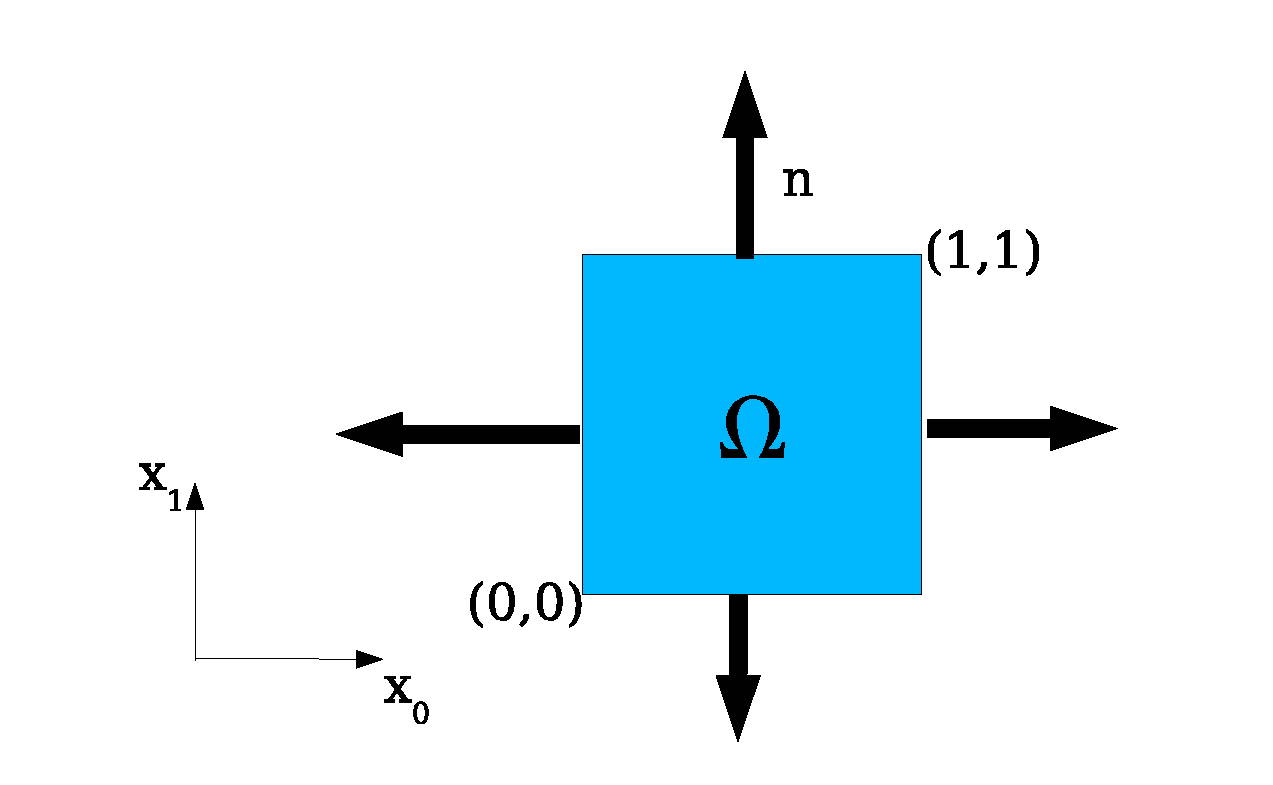
\includegraphics{FirstStepDomain}}
    \caption{Domain $\Omega=[0,1]^2$ with outer normal field $n$.}
    \label{fig:FirstSteps.1}
\end{figure}

$\Delta$ denotes the Laplace operator\index{Laplace operator}, which is defined by
\begin{equation}
\Delta u = (u\hackscore {,0})\hackscore{,0}+(u\hackscore{,1})\hackscore{,1}
\label{eq:FirstSteps.1.1}
\end{equation}
where, for any function $u$ and any direction $i$, $u\hackscore{,i}$
denotes the partial derivative \index{partial derivative} of $u$ with respect
to $i$.\footnote{You may be more familiar with the Laplace
operator\index{Laplace operator} being written as $\nabla^2$, and written in
the form
\begin{equation*}
    \nabla^2 u = \nabla^t \cdot \nabla u =  \frac{\partial^2 u}{\partial x\hackscore 0^2} 
    + \frac{\partial^2 u}{\partial  x\hackscore 1^2}
\end{equation*}
and \eqn{eq:FirstSteps.1} as
\begin{equation*}
    -\nabla^2 u = f
\end{equation*}
}
Basically, in the subindex of a function, any index to the left of the comma denotes a spatial derivative with respect 
to the index. To get a more compact form we will write $u\hackscore{,ij}=(u\hackscore {,i})\hackscore{,j}$
which leads to
\begin{equation}
\Delta u = u\hackscore{,00}+u\hackscore{,11}=\sum\hackscore{i=0}^2 u\hackscore{,ii}
\label{eq:FirstSteps.1.1b}
\end{equation}
We often find that use
of nested $\sum$ symbols makes formulas cumbersome, and we use the more
convenient Einstein summation convention\index{summation convention}. This 
drops the $\sum$ sign and assumes that a summation is performed over any repeated index.
For instance we write
\begin{eqnarray}
x\hackscore{i}y\hackscore{i}=\sum\hackscore{i=0}^2 x\hackscore{i}y\hackscore{i}   \\
x\hackscore{i}u\hackscore{,i}=\sum\hackscore{i=0}^2 x\hackscore{i}u\hackscore{,i}   \\
u\hackscore{,ii}=\sum\hackscore{i=0}^2 u\hackscore{,ii} \\
x\hackscore{ij}u\hackscore{i,j}=\sum\hackscore{j=0}^2\sum\hackscore{i=0}^2 x\hackscore{ij}u\hackscore{i,j}   \\
\label{eq:FirstSteps.1.1c}
\end{eqnarray}
With the summation convention we can write the Poisson equation \index{Poisson equation} as
\begin{equation}
- u\hackscore{,ii} =1 
\label{eq:FirstSteps.1.sum}
\end{equation}
where $f=1$ in this example.

On the boundary of the domain $\Omega$ the normal derivative $n\hackscore{i} u\hackscore{,i}$
of the solution $u$ shall be zero, i.e. $u$ shall fulfill
the homogeneous Neumann boundary condition\index{Neumann
boundary condition!homogeneous}
\begin{equation}
n\hackscore{i} u\hackscore{,i}= 0 \;.
\label{eq:FirstSteps.2}
\end{equation}
$n=(n\hackscore{i})$ denotes the outer normal field
of the domain, see \fig{fig:FirstSteps.1}. Remember that we 
are applying the Einstein summation convention \index{summation convention}, i.e. $n\hackscore{i} u\hackscore{,i}= n\hackscore{0} u\hackscore{,0} +%
n\hackscore{1} u\hackscore{,1}$.\footnote{Some readers may familiar with the
notation $\frac{\partial u}{\partial n} = n\hackscore{i} u\hackscore{,i}$
for the normal derivative.}
The Neumann boundary condition of \eqn{eq:FirstSteps.2} should be fulfilled on the
set $\Gamma^N$ which is the top and right edge of the domain:
\begin{equation}
    \Gamma^N=\{(x\hackscore 0;x\hackscore 1) \in \Omega | x\hackscore{0}=1 \mbox{ or } x\hackscore{1}=1  \}
    \label{eq:FirstSteps.2b}
\end{equation}
On the bottom and the left edge of the domain which is defined
as 
\begin{equation}
    \Gamma^D=\{(x\hackscore 0;x\hackscore 1) \in \Omega | x\hackscore{0}=0 \mbox{ or } x\hackscore{1}=0  \}
    \label{eq:FirstSteps.2c}
\end{equation}
the solution shall be identical to zero:
\begin{equation}
    u=0 \; .
    \label{eq:FirstSteps.2d}
\end{equation}
This kind of boundary condition is called a homogeneous Dirichlet boundary
condition\index{Dirichlet boundary condition!homogeneous}.
The partial differential equation in \eqn{eq:FirstSteps.1.sum} together
with the Neumann boundary condition \eqn{eq:FirstSteps.2} and 
Dirichlet boundary condition in \eqn{eq:FirstSteps.2d} form a so-called
boundary value
problem\index{boundary value problem} (BVP\index{boundary value problem!BVP})
for the unknown function~$u$. 

\begin{figure}[ht]
    \centerline{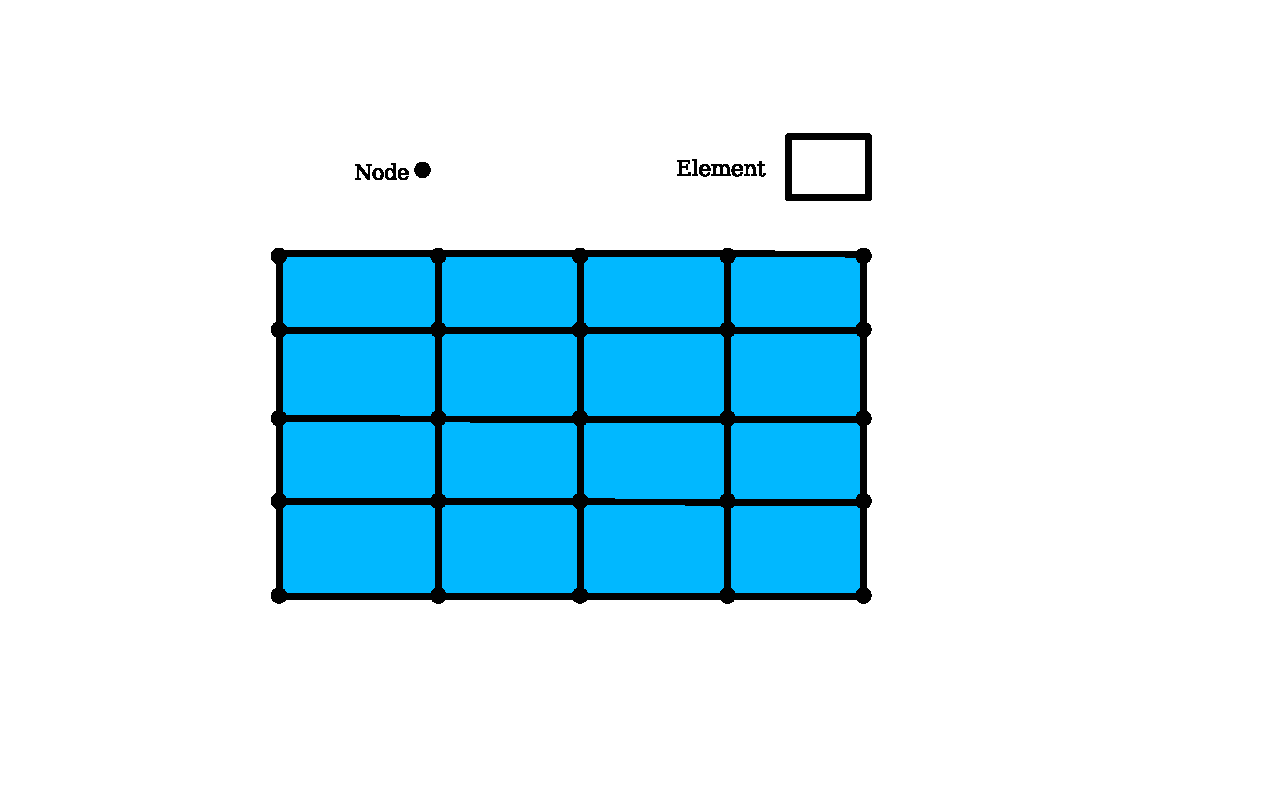
\includegraphics{FirstStepMesh}}
    \caption{Mesh of $4 \times 4$ elements on a rectangular domain. Here
    each element is a quadrilateral and described by four nodes, namely
    the corner points. The solution is interpolated by a bi-linear
    polynomial.}
    \label{fig:FirstSteps.2}
\end{figure}

In general the BVP\index{boundary value problem!BVP} cannot be solved
analytically and numerical methods have to be used to construct an
approximation of the solution $u$.
Here we will use the finite element method\index{finite element method}
(FEM\index{finite element method!FEM}).
The basic idea is to fill the domain with a set of points called nodes.
The solution is approximated by its values on the nodes\index{finite element method!nodes}.
Moreover, the domain is subdivided into smaller sub-domains called
elements\index{finite element method!element}.
On each element the solution is represented by a polynomial of a certain
degree through its values at the nodes located in the element.
The nodes and their connection through elements is called a
mesh\index{finite element method!mesh}. \fig{fig:FirstSteps.2} shows an
example of a FEM mesh with four elements in the $x_0$ and four elements
in the $x_1$ direction over the unit square.
For more details we refer the reader to the literature, for instance \Ref{Zienc,NumHand}.

The \escript solver we want to use to solve this problem is embedded into the python interpreter language.
So you can solve the problem interactively but you will learn quickly that it
is more efficient to use scripts which you can edit with your favorite editor.
To enter the escript environment, use the \program{run-escript}
command\footnote{\program{run-escript} is not available under Windows yet.
If you run under Windows you can just use the \program{python} command and the
\env{OMP_NUM_THREADS} environment variable to control the number of threads.}:
\begin{verbatim}
run-escript
\end{verbatim}
which will pass you on to the python prompt
\begin{verbatim}
Python 2.5.2 (r252:60911, Oct  5 2008, 19:29:17) 
[GCC 4.3.2] on linux2
Type "help", "copyright", "credits" or "license" for more information.
>>> 
\end{verbatim}
Here you can use all available python commands and language features, for instance
\begin{python}
  >>> x=2+3
  >>> print "2+3=",x
  2+3= 5
\end{python}
We refer to the python user's guide if you not familiar with python.

\escript provides the class \Poisson to define a Poisson equation\index{Poisson equation}.
(We will discuss a more general form of a PDE\index{partial differential equation!PDE} 
that can be defined through the \LinearPDE class later.)
The instantiation of a \Poisson class object requires the specification of the domain $\Omega$.
In \escript the \Domain class objects are used to describe the geometry of a
domain but it also contains information about the discretization methods and
the actual solver which is used to solve the PDE.
Here we are using the FEM library \finley\index{finite element method}.
The following statements create the \Domain object \var{mydomain} from the 
\finley method \method{Rectangle}:
\begin{python}
  from esys.finley import Rectangle
  mydomain = Rectangle(l0=1.,l1=1.,n0=40, n1=20)
\end{python}
In this case the domain is a rectangle with the lower, left corner at point $(0,0)$ and
the right, upper corner at $(\var{l0},\var{l1})=(1,1)$.
The arguments \var{n0} and \var{n1} define the number of elements in $x\hackscore{0}$ and
$x\hackscore{1}$-direction respectively. For more details on \method{Rectangle} and
other \Domain generators within the \finley module,
see \Chap{CHAPTER ON FINLEY}.

The following statements define the \Poisson class object \var{mypde} with domain \var{mydomain} and
the right hand side $f$ of the PDE to constant $1$: 
\begin{python}
  from esys.escript.linearPDEs import Poisson
  mypde = Poisson(mydomain)
  mypde.setValue(f=1)
\end{python}
We have not specified any boundary condition but the \Poisson class implicitly
assumes homogeneous Neuman boundary conditions\index{Neumann boundary condition!homogeneous} defined by \eqn{eq:FirstSteps.2}.
With this boundary condition the BVP\index{boundary value problem!BVP} we have
defined has no unique solution.
In fact, with any solution $u$ and any constant $C$ the function $u+C$ becomes
a solution as well.
We have to add a Dirichlet boundary condition\index{Dirichlet boundary condition}.
This is done by defining a characteristic function\index{characteristic function}
which has positive values at locations $x=(x\hackscore{0},x\hackscore{1})$
where Dirichlet boundary condition is set and $0$ elsewhere.
In our case of $\Gamma^D$ defined by \eqn{eq:FirstSteps.2c}, we need to
construct a function \var{gammaD} which is positive for the cases $x\hackscore{0}=0$ or $x\hackscore{1}=0$.
To get an object \var{x} which contains the coordinates of the nodes in the domain use
\begin{python}
  x=mydomain.getX() 
\end{python}
The method \method{getX} of the \Domain \var{mydomain} gives access to locations
in the domain defined by \var{mydomain}.
The object \var{x} is actually a \Data object which will be discussed in
\Chap{ESCRIPT CHAP} in more detail.
What we need to know here is that \var{x} has \Rank (number of dimensions) and
a \Shape (list of dimensions) which can be viewed by calling the \method{getRank} and \method{getShape} methods:
\begin{python}
  print "rank ",x.getRank(),", shape ",x.getShape()
\end{python}
This will print something like
\begin{python}
  rank 1, shape (2,)
\end{python}
The \Data object also maintains type information which is represented by the 
\FunctionSpace of the object. For instance
\begin{python}
  print x.getFunctionSpace()
\end{python}
will print 
\begin{python}
  Function space type: Finley_Nodes on FinleyMesh 
\end{python}
which tells us that the coordinates are stored on the nodes of (rather than on
points in the interior of) a \finley mesh.
To get the  $x\hackscore{0}$ coordinates of the locations we use the statement 
\begin{python}
  x0=x[0]
\end{python}
Object \var{x0} is again a \Data object now with \Rank $0$ and \Shape $()$.
It inherits the \FunctionSpace from \var{x}:
\begin{python}
  print x0.getRank(), x0.getShape(), x0.getFunctionSpace()
\end{python}
will print
\begin{python}
  0 () Function space type: Finley_Nodes on FinleyMesh 
\end{python}
We can now construct a function \var{gammaD} which is only non-zero on the
bottom and left edges of the domain with
\begin{python}
  from esys.escript import whereZero
  gammaD=whereZero(x[0])+whereZero(x[1])
\end{python}

\code{whereZero(x[0])} creates a function which equals $1$ where \code{x[0]} is (almost) equal to zero and $0$ elsewhere. 
Similarly, \code{whereZero(x[1])} creates a function which equals $1$ where \code{x[1]} is equal to zero and $0$ elsewhere.
The sum of the results of \code{whereZero(x[0])} and \code{whereZero(x[1])}
gives a function on the domain \var{mydomain} which is strictly positive where $x\hackscore{0}$ or $x\hackscore{1}$ is equal to zero.
Note that \var{gammaD} has the same \Rank, \Shape and \FunctionSpace like \var{x0} used to define it.
So from 
\begin{python}
  print gammaD.getRank(), gammaD.getShape(), gammaD.getFunctionSpace()
\end{python}
one gets 
\begin{python}
  0 () Function space type: Finley_Nodes on FinleyMesh 
\end{python}
An additional parameter \var{q} of the \code{setValue} method of the \Poisson
class defines the characteristic function\index{characteristic function} of
the locations of the domain where the homogeneous Dirichlet boundary condition\index{Dirichlet boundary condition!homogeneous} is set.
The complete definition of our example is now:
\begin{python}
  from esys.escript.linearPDEs import Poisson
  x = mydomain.getX()
  gammaD = whereZero(x[0])+whereZero(x[1])
  mypde = Poisson(domain=mydomain)
  mypde.setValue(f=1,q=gammaD)
\end{python}
The first statement imports the \Poisson class definition from the \linearPDEs module.
To get the solution of the Poisson equation defined by \var{mypde} we just have to call its \method{getSolution} method. 

Now we can write the script to solve our Poisson problem
\begin{python}
  from esys.escript import *
  from esys.escript.linearPDEs import Poisson
  from esys.finley import Rectangle
  # generate domain:
  mydomain = Rectangle(l0=1.,l1=1.,n0=40, n1=20)
  # define characteristic function of Gamma^D
  x = mydomain.getX()
  gammaD = whereZero(x[0])+whereZero(x[1])
  # define PDE and get its solution u
  mypde = Poisson(domain=mydomain)
  mypde.setValue(f=1,q=gammaD)
  u = mypde.getSolution()
\end{python}
The question is what we do with the calculated solution \var{u}.
Besides postprocessing, e.g. calculating the gradient or the average value, which will be discussed later, plotting the solution is one of the things you might want to do.
\escript offers two ways to do this, both based on external modules or packages and so data need to converted to hand over the solution.
The first option is using the \MATPLOTLIB module which allows plotting 2D results relatively quickly from within the Python script, see~\cite{matplotlib}.
However, there are limitations when using this tool, especially for large problems and when solving 3-dimensional problems.
Therefore, \escript provides functionality to export data as files which can subsequently be read by third-party software packages such as \mayavi\cite{mayavi} or \VisIt~\cite{VisIt}.

\subsection{Plotting Using \MATPLOTLIB}
The \MATPLOTLIB module provides a simple and easy-to-use way to visualize PDE solutions (or other \Data objects).
To hand over data from \escript to \MATPLOTLIB the values need to mapped onto
a rectangular grid\footnote{Users of Debian 5 (Lenny) please note: this example
makes use of the \function{griddata} method in \module{matplotlib.mlab}.
This method is not part of version 0.98.1 which is available with Lenny.
If you wish to use contour plots, you may need to install a later version.
Users of Ubuntu 8.10 or later should be fine.}. We will make use of the \numpy module.

First we need to create a rectangular grid which is accomplished by the following statements:
\begin{python}
  import numpy
  x_grid = numpy.linspace(0., 1., 50)
  y_grid = numpy.linspace(0., 1., 50)
\end{python}
\var{x_grid} is an array defining the x coordinates of the grid while
\var{y_grid} defines the y coordinates of the grid.
In this case we use $50$ points over the interval $[0,1]$ in both directions. 

Now the values created by \escript need to be interpolated to this grid.
We will use the \MATPLOTLIB \function{mlab.griddata} function to do this.
Spatial coordinates are easily extracted as a \var{list} by
\begin{python}
  x=mydomain.getX()[0].toListOfTuples()
  y=mydomain.getX()[1].toListOfTuples()
\end{python}
In principle we can apply the same \member{toListOfTuples} method to extract the values from the PDE solution \var{u}.
However, we have to make sure that the \Data object we extract the values from
uses the same \FunctionSpace as we have used when extracting \var{x} and \var{y}.
We apply the \function{interpolation} to \var{u} before extraction to achieve this:
\begin{python}
  z=interpolate(u, mydomain.getX().getFunctionSpace())
\end{python}
The values in \var{z} are the values at the points with the coordinates given by \var{x} and \var{y}.
These values are interpolated to the grid defined by \var{x_grid} and \var{y_grid} by using
\begin{python}
  import matplotlib
  z_grid = matplotlib.mlab.griddata(x, y, z, xi=x_grid, yi=y_grid)
\end{python}
Now \var{z_grid} gives the values of the PDE solution \var{u} at the grid which can be plotted using \function{contourf}:
\begin{python}
  matplotlib.pyplot.contourf(x_grid, y_grid, z_grid, 5)
  matplotlib.pyplot.savefig("u.png")
\end{python}
Here we use 5 contours. The last statement writes the plot to the file \file{u.png} in the PNG format.
Alternatively, one can use 
\begin{python}
  matplotlib.pyplot.contourf(x_grid, y_grid, z_grid, 5)
  matplotlib.pyplot.show()
\end{python}
which gives an interactive browser window.

\begin{figure}
\centerline{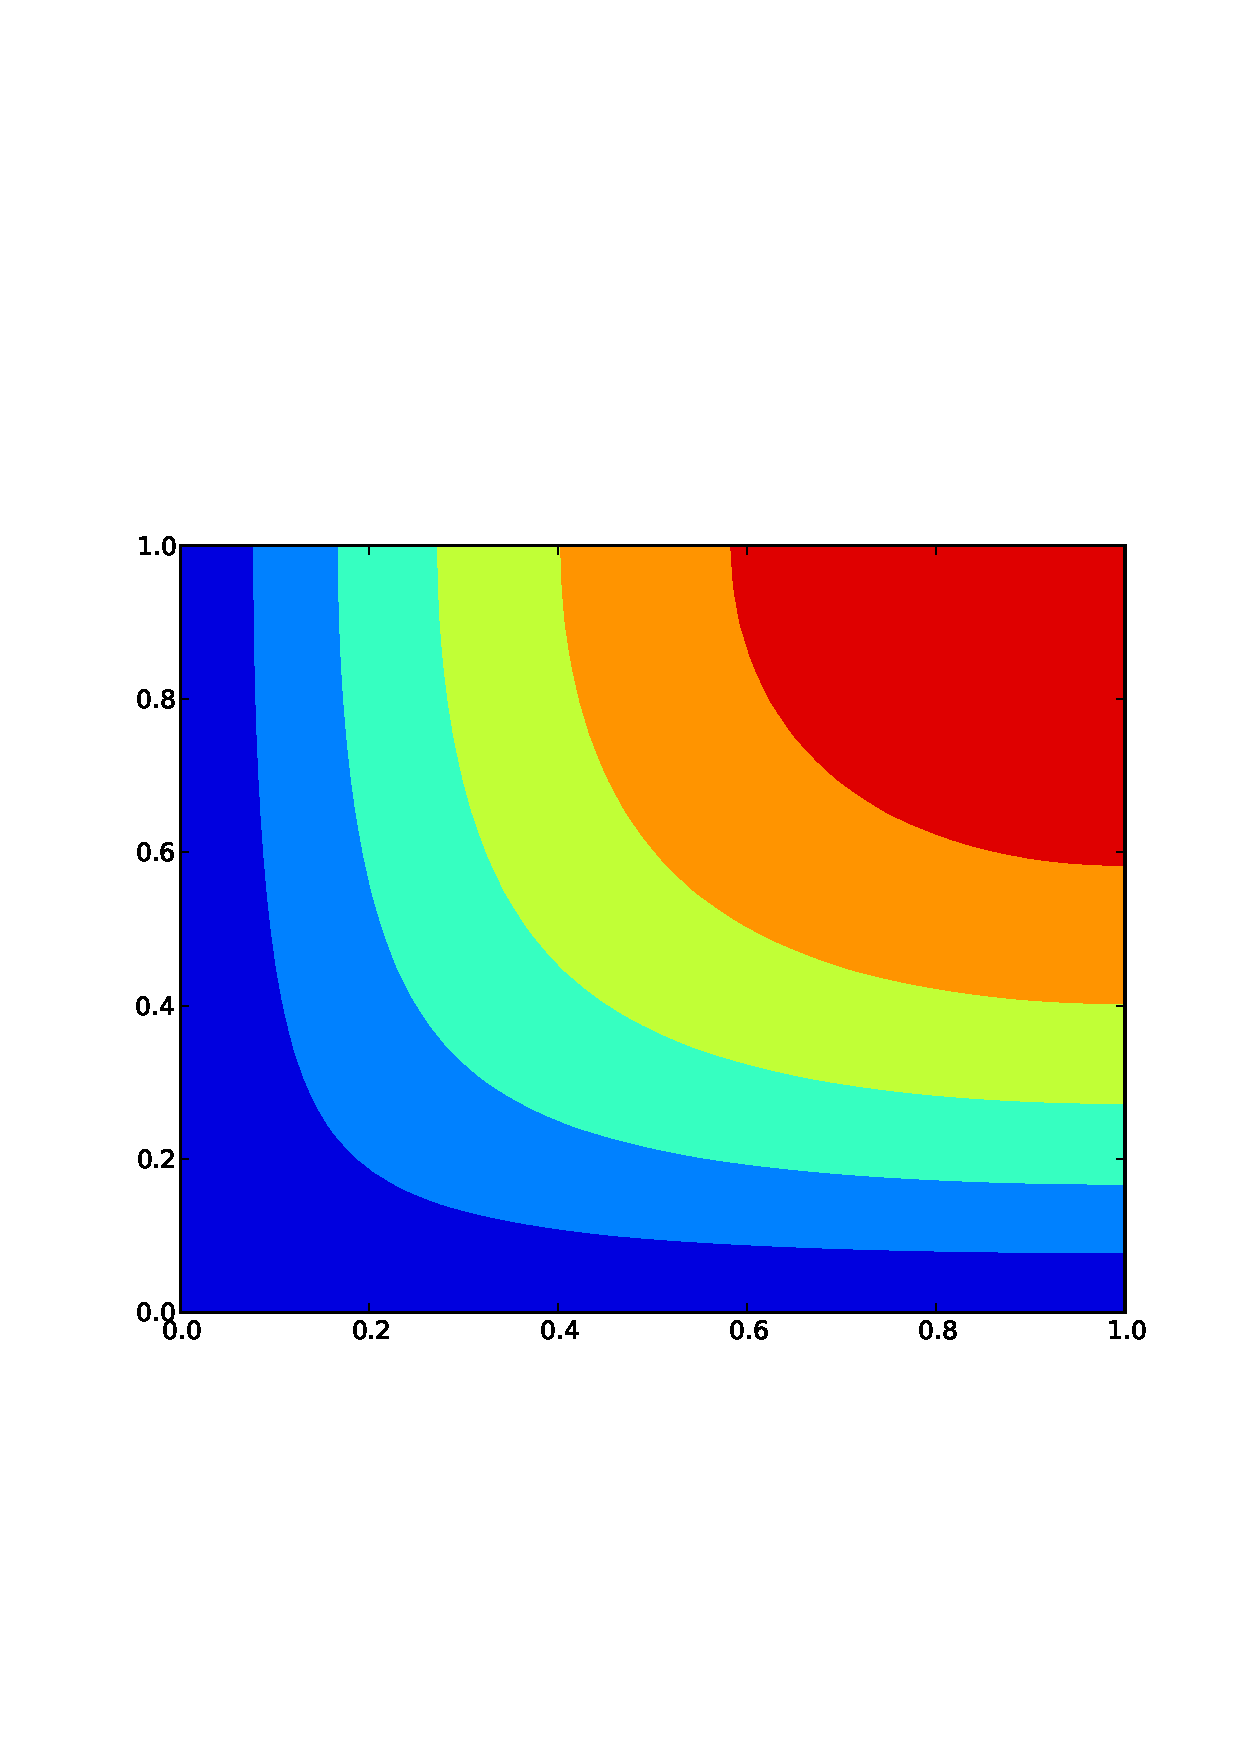
\includegraphics[width=\figwidth]{FirstStepResultMATPLOTLIB}}
\caption{Visualization of the Poisson Equation Solution for $f=1$ using \MATPLOTLIB}
\label{fig:FirstSteps.3b}
\end{figure}

Now we can write the script to solve our Poisson problem
\begin{python}
  from esys.escript import *
  from esys.escript.linearPDEs import Poisson
  from esys.finley import Rectangle
  import numpy
  import matplotlib
  import pylab
  # generate domain:
  mydomain = Rectangle(l0=1.,l1=1.,n0=40, n1=20)
  # define characteristic function of Gamma^D
  x = mydomain.getX()
  gammaD = whereZero(x[0])+whereZero(x[1])
  # define PDE and get its solution u
  mypde = Poisson(domain=mydomain)
  mypde.setValue(f=1,q=gammaD)
  u = mypde.getSolution()
  # interpolate u to a matplotlib grid:
  x_grid = numpy.linspace(0.,1.,50)
  y_grid = numpy.linspace(0.,1.,50)
  x=mydomain.getX()[0].toListOfTuples()
  y=mydomain.getX()[1].toListOfTuples()
  z=interpolate(u,mydomain.getX().getFunctionSpace())
  z_grid = matplotlib.mlab.griddata(x,y,z,xi=x_grid,yi=y_grid )
  # interpolate u to a rectangular grid:
  matplotlib.pyplot.contourf(x_grid, y_grid, z_grid, 5)
  matplotlib.pyplot.savefig("u.png")
\end{python}
The entire code is available as \file{poisson\hackscore matplotlib.py} in the \ExampleDirectory.
You can run the script using the {\it escript} environment
\begin{verbatim}
run-escript poisson_matplotlib.py
\end{verbatim}
This will create the \file{u.png}, see \fig{fig:FirstSteps.3b}.
For details on the usage of the \MATPLOTLIB module we refer to the documentation~\cite{matplotlib}.

As pointed out, \MATPLOTLIB is restricted to the two-dimensional case and
should be used for small problems only.
It can not be used under \MPI as the \member{toListOfTuples} method is not
safe under \MPI\footnote{The phrase 'safe under \MPI' means that a program
will produce correct results when run on more than one processor under \MPI.}.

\begin{figure}
\centerline{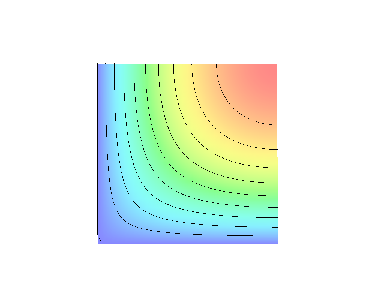
\includegraphics[width=\figwidth]{FirstStepResult}}
\caption{Visualization of the Poisson Equation Solution for $f=1$}
\label{fig:FirstSteps.3}
\end{figure}

\subsection{Visualization using export files}

As an alternative to \MATPLOTLIB, {\it escript} supports exporting data to
\VTK and \SILO files which can be read by visualization tools such as
mayavi\cite{mayavi} and \VisIt~\cite{VisIt}. This method is \MPI safe and
works with large 2D and 3D problems.

To write the solution \var{u} of the Poisson problem in the \VTK file format
to the file \file{u.vtu} one needs to add:
\begin{python}
  saveVTK("u.vtu", sol=u)
\end{python}
This file can then be opened in a \VTK compatible visualization tool where the
solution is accessible by the name {\it sol}.

The Poisson problem script is now 
\begin{python}
  from esys.escript import *
  from esys.escript.linearPDEs import Poisson
  from esys.finley import Rectangle
  # generate domain:
  mydomain = Rectangle(l0=1.,l1=1.,n0=40, n1=20)
  # define characteristic function of Gamma^D
  x = mydomain.getX()
  gammaD = whereZero(x[0])+whereZero(x[1])
  # define PDE and get its solution u
  mypde = Poisson(domain=mydomain)
  mypde.setValue(f=1,q=gammaD)
  u = mypde.getSolution()
  # write u to an external file
  saveVTK("u.vtu",sol=u)
\end{python}
The entire code is available as \file{poisson\hackscore vtk.py} in the \ExampleDirectory.

You can run the script using the {\it escript} environment and visualize the
solution using \mayavi:
\begin{verbatim}
run-escript poisson_vtk.py
mayavi2 -d u.vtu -m SurfaceMap
\end{verbatim}
The result is shown in \fig{fig:FirstSteps.3}.



%%%%%%%%%%%%%%%%%%%%%%%%%%%%%%%%%%%%%%%%%%%%%%%%%%%%%%%%
%
% Copyright (c) 2003-2008 by University of Queensland
% Earth Systems Science Computational Center (ESSCC)
% http://www.uq.edu.au/esscc
%
% Primary Business: Queensland, Australia
% Licensed under the Open Software License version 3.0
% http://www.opensource.org/licenses/osl-3.0.php
%
%%%%%%%%%%%%%%%%%%%%%%%%%%%%%%%%%%%%%%%%%%%%%%%%%%%%%%%%


\section{The Diffusion Problem}
\label{DIFFUSION CHAP}

\begin{figure}
\centerline{\includegraphics[width=\figwidth]{figures/DiffusionDomain.eps}}
\caption{Temperature Diffusion Problem with Circular Heat Source}
\label{DIFFUSION FIG 1}
\end{figure}

\subsection{\label{DIFFUSION OUT SEC}Outline}
In this chapter we will discuss how to solve a time-dependent temperature diffusion\index{diffusion equation} PDE for
a given block of material. Within the block there is a heat source which drives the temperature diffusion.
On the surface, energy can radiate into the surrounding environment.
\fig{DIFFUSION FIG 1} shows the configuration.

In the next \Sec{DIFFUSION TEMP SEC} we will present the relevant model. A 
time integration scheme is introduced to calculate the temperature at given time nodes $t^{(n)}$. 
We will see that at each time step a Helmholtz equation \index{Helmholtz equation} 
must be solved. 
The implementation of a Helmholtz equation solver will be discussed in \Sec{DIFFUSION HELM SEC}. 
In Section~\ref{DIFFUSION TRANS SEC} the solver of the Helmholtz equation is used to build a
solver for the temperature diffusion problem. 

\subsection{\label{DIFFUSION TEMP SEC}Temperature Diffusion}
The unknown temperature $T$ is a function of its location in the domain and time $t>0$. The governing equation
in the interior of the domain is given by
\begin{equation}
\rho c\hackscore p T\hackscore{,t} - (\kappa T\hackscore{,i})\hackscore{,i} = q\hackscore H
\label{DIFFUSION TEMP EQ 1}
\end{equation}
where $\rho c\hackscore p$ and $\kappa$ are given material constants. In case of a composite
material the parameters depend on their location in the domain. $q\hackscore H$ is
a heat source (or sink) within the domain. We are using the Einstein summation convention \index{summation convention} 
as introduced in \Chap{FirstSteps}. In our case we assume $q\hackscore H$ to be equal to a constant heat production rate 
$q^{c}$ on a circle or sphere with center $x^c$ and radius $r$ and $0$ elsewhere:
\begin{equation}
q\hackscore H(x,t)=
\left\{ 
\begin{array}{lcl}
q^c  & & \|x-x^c\| \le r \\
     & \mbox{if} \\
0    &  & \mbox{else} \\
\end{array}
\right.
\label{DIFFUSION TEMP EQ 1b}
\end{equation}
for all $x$ in the domain and all time  $t>0$.

On the surface of the domain we are 
specifying a radiation condition 
which prescribes the normal component of the flux $\kappa T\hackscore{,i}$ to be proportional
to the difference of the current temperature to the surrounding temperature $T\hackscore{ref}$:    
\begin{equation}
 \kappa T\hackscore{,i} n\hackscore i = \eta (T\hackscore{ref}-T) 
\label{DIFFUSION TEMP EQ 2}
\end{equation}
$\eta$ is a given material coefficient depending on the material of the block and the surrounding medium. 
$n\hackscore i$ is the $i$-th component of the outer normal field \index{outer normal field}
at the surface of the domain. 

To solve the time-dependent \eqn{DIFFUSION TEMP EQ 1} the initial temperature at time 
$t=0$ has to be given. Here we assume that the initial temperature is the surrounding temperature:
\begin{equation}
T(x,0)=T\hackscore{ref} 
\label{DIFFUSION TEMP EQ 4}
\end{equation}
for all $x$ in the domain. It is pointed out that 
the initial conditions satisfy the 
boundary condition defined by \eqn{DIFFUSION TEMP EQ 2}. 

The temperature is calculated at discrete time nodes $t^{(n)}$ where 
$t^{(0)}=0$ and  $t^{(n)}=t^{(n-1)}+h$ where $h>0$ is the step size which is assumed to be constant. 
In the following the upper index ${(n)}$ refers to a value at time $t^{(n)}$. The simplest
and most robust scheme to approximate the time derivative of the the temperature is 
the backward Euler
\index{backward Euler} scheme. The backward Euler 
scheme is based
on the Taylor expansion of $T$ at time $t^{(n)}$:
\begin{equation}
T^{(n)}\approx T^{(n-1)}+T\hackscore{,t}^{(n)}(t^{(n)}-t^{(n-1)})
=T^{(n-1)} + h \cdot T\hackscore{,t}^{(n)}
\label{DIFFUSION TEMP EQ 6}
\end{equation}
This is inserted into \eqn{DIFFUSION TEMP EQ 1}. By separating the terms at 
$t^{(n)}$ and  $t^{(n-1)}$ one gets for $n=1,2,3\ldots$
\begin{equation}
\frac{\rho c\hackscore p}{h} T^{(n)} - (\kappa T^{(n)}\hackscore{,i})\hackscore{,i} = q\hackscore H +  \frac{\rho c\hackscore p}{h} T^{(n-1)}
\label{DIFFUSION TEMP EQ 7}
\end{equation}
where $T^{(0)}=T\hackscore{ref}$ is taken form the initial condition given by \eqn{DIFFUSION TEMP EQ 4}.
Together with the natural boundary condition 
\begin{equation}
 \kappa T\hackscore{,i}^{(n)} n\hackscore i = \eta (T\hackscore{ref}-T^{(n)}) 
\label{DIFFUSION TEMP EQ 2222}
\end{equation}
taken from \eqn{DIFFUSION TEMP EQ 2}
this forms a boundary value problem that has to be solved for each time step. 
As a first step to implement a solver for the temperature diffusion problem we will 
first implement a solver for the  boundary value problem that has to be solved at each time step.

\subsection{\label{DIFFUSION HELM SEC}Helmholtz Problem}
The partial differential equation to be solved for $T^{(n)}$ has the form 
\begin{equation}
\omega T^{(n)}  - (\kappa T^{(n)}\hackscore{,i})\hackscore{,i} = f
\label{DIFFUSION HELM EQ 1}
\end{equation}
and we set
\begin{equation}
\omega=\frac{\rho c\hackscore p}{h} \mbox{ and } f=q\hackscore H +\frac{\rho c\hackscore p}{h}T^{(n-1)} \;.
\label{DIFFUSION HELM EQ 1b}
\end{equation}
With $g=\eta T\hackscore{ref}$ the radiation condition defined by \eqn{DIFFUSION TEMP EQ 2222}
takes the form 
\begin{equation}
\kappa T^{(n)}\hackscore{,i} n\hackscore{i} =  g - \eta T^{(n)}\mbox{ on } \Gamma
\label{DIFFUSION HELM EQ 2}
\end{equation}
The partial differential \eqn{DIFFUSION HELM EQ 1} together with boundary conditions of \eqn{DIFFUSION HELM EQ 2}
is called the Helmholtz equation \index{Helmholtz equation}. 

We want to use the \LinearPDE class provided by \escript to define and solve a general linear,steady, second order PDE such as the 
Helmholtz equation. For a single PDE the \LinearPDE class supports the following form:
\begin{equation}\label{LINEARPDE.SINGLE.1 TUTORIAL}
-(A\hackscore{jl} u\hackscore{,l})\hackscore{,j}+D u = Y \; .
\end{equation}
where we show only the coefficients relevant for the problem discussed here. For the general form of 
single PDE see \eqn{LINEARPDE.SINGLE.1}. 
The coefficients $A$, and $Y$ have to be specified through \Data objects in the 
\Function on the PDE or objects that can be converted into such \Data objects. 
$A$ is a \RankTwo and $D$ and $Y$ are scalar. 
The following natural
boundary conditions are considered \index{boundary condition!natural} on $\Gamma$:
\begin{equation}\label{LINEARPDE.SINGLE.2 TUTORIAL}
n\hackscore{j}A\hackscore{jl} u\hackscore{,l}+d u= y  \;.
\end{equation}
Notice that the coefficient $A$ is the same like in the PDE~\eqn{LINEARPDE.SINGLE.1 TUTORIAL}. 
The coefficients $d$ and $y$ are  
each a \Scalar in the \FunctionOnBoundary.  Constraints \index{constraint} for the solution prescribing the value of the 
solution at certain locations in the domain. They have the form
\begin{equation}\label{LINEARPDE.SINGLE.3 TUTORIAL}
u=r \mbox{ where } q>0
\end{equation}
$r$ and $q$ are each \Scalar where $q$ is the characteristic function
\index{characteristic function} defining where the constraint is applied.
The constraints defined by \eqn{LINEARPDE.SINGLE.3  TUTORIAL} override any other condition set by 
\eqn{LINEARPDE.SINGLE.1 TUTORIAL} or \eqn{LINEARPDE.SINGLE.2 TUTORIAL}. 
The \Poisson class of the \linearPDEs module,
which we have already used in \Chap{FirstSteps}, is in fact a subclass of the more general
\LinearPDE class. The \linearPDEs module provides a \Helmholtz class but
we will make direct use of the general \LinearPDE class.

By inspecting the Helmholtz equation \index{Helmholtz equation} 
(\ref{DIFFUSION HELM EQ 1}) and boundary condition (\ref{DIFFUSION HELM EQ 2}) and 
substituting $u$ for $T^{(n)}$ 
we can easily assign values to the coefficients in the 
general PDE of the \LinearPDE class:
\begin{equation}\label{DIFFUSION HELM EQ 3}
\begin{array}{llllll}
A\hackscore{ij}=\kappa \delta\hackscore{ij} & D=\omega & Y=f \\
d=\eta & y= g &  \\
\end{array}
\end{equation}
$\delta\hackscore{ij}$ is the Kronecker symbol \index{Kronecker symbol} defined by $\delta\hackscore{ij}=1$ for
$i=j$ and $0$ otherwise. Undefined coefficients are assumed to be not present.\footnote{There is a difference 
in \escript of being not present and set to zero. As not present coefficients are not processed, 
it is more efficient to leave a coefficient undefined instead of assigning zero to it.} 
In this diffusion example we do not need to define a characteristic function $q$ because the 
boundary conditions we consider in \eqn{DIFFUSION HELM EQ 2} are just the natural boundary 
conditions which are already defined in the \LinearPDE class (shown in \eqn{LINEARPDE.SINGLE.2 TUTORIAL}).

The Helmholtz equation can be set up by following way~\footnote{Please, note that this is not a complete code. The complete code can be found in ``helmholtz.py''. } :
\begin{python}
mypde=LinearPDE(mydomain)
mypde.setValue(A=kappa*kronecker(mydomain),D=omega,Y=f,d=eta,y=g)
u=mypde.getSolution()
\end{python}
where we assume that \code{mydomain} is a \Domain object and 
\code{kappa} \code{omega} \code{eta} and \code{g} are given scalar values 
typically \code{float} or \Data objects. The \method{setValue} method 
assigns values to the coefficients of the general PDE. The \method{getSolution} method solves 
the PDE and returns the solution \code{u} of the PDE. \function{kronecker} is \escript function
returning the Kronecker symbol.

The coefficients can set by several calls of \method{setValue} where the order can be chosen arbitrarily. 
If a value is assigned to a coefficient several times, the last assigned value is used when
the solution is calculated:
\begin{python}
mypde=LinearPDE(mydomain)
mypde.setValue(A=kappa*kronecker(mydomain),d=eta)
mypde.setValue(D=omega,Y=f,y=g)
mypde.setValue(d=2*eta) # overwrites d=eta
u=mypde.getSolution()
\end{python}
In some cases the solver of the PDE can make use of the fact that the PDE is symmetric\index{symmetric PDE} where the 
PDE is called symmetric if 
\begin{equation}\label{LINEARPDE.SINGLE.4  TUTORIAL}
A\hackscore{jl}=A\hackscore{lj}\;.
\end{equation}
Note that $D$ and $d$ may have any value and the right hand sides $Y$, $y$ as well as the constraints
are not relevant. The Helmholtz problem is symmetric. 
The \LinearPDE class provides the method \method{checkSymmetry} method to check if the given PDE is symmetric. 
\begin{python}
mypde=LinearPDE(mydomain)
mypde.setValue(A=kappa*kronecker(mydomain),d=eta)
print mypde.checkSymmetry() # returns True
mypde.setValue(B=kronecker(mydomain)[0])
print mypde.checkSymmetry() # returns False
mypde.setValue(C=kronecker(mydomain)[0])
print mypde.checkSymmetry() # returns True
\end{python}
Unfortunately, a \method{checkSymmetry} is very expensive and is recommendable to use for
testing and debugging purposes only. The \method{setSymmetryOn} method is used to
declare a PDE symmetric:
\begin{python}
mypde = LinearPDE(mydomain)
mypde.setValue(A=kappa*kronecker(mydomain))
mypde.setSymmetryOn()
\end{python}
Now we want to see how we actually solve the Helmholtz equation.
on a rectangular domain
of length $l\hackscore{0}=5$ and height $l\hackscore{1}=1$. We choose a simple test solution such that we 
can verify the returned solution against the exact answer. Actually, we 
take $T=x\hackscore{0}$ (here $q\hackscore H = 0$) and then calculate the right hand side terms $f$ and $g$ such that
the test solution becomes the solution of the problem. If we assume $\kappa$ as being constant, 
an easy calculation shows that we have to choose $f=\omega \cdot x\hackscore{0}$. On the boundary we get
$\kappa n\hackscore{i} u\hackscore{,i}=\kappa n\hackscore{0}$.  
So we have to set $g=\kappa n\hackscore{0}+\eta x\hackscore{0}$. The following script \file{helmholtz.py} 
\index{scripts!\file{helmholtz.py}} which is available in the \ExampleDirectory
implements this test problem using the \finley PDE solver:
\begin{python}
from esys.escript import *
from esys.escript.linearPDEs import LinearPDE
from esys.finley import Rectangle
#... set some parameters ...
kappa=1.
omega=0.1
eta=10.
#... generate domain ...
mydomain = Rectangle(l0=5.,l1=1.,n0=50, n1=10)
#... open PDE and set coefficients ...
mypde=LinearPDE(mydomain)
mypde.setSymmetryOn()
n=mydomain.getNormal()
x=mydomain.getX()
mypde.setValue(A=kappa*kronecker(mydomain),D=omega,Y=omega*x[0], \
               d=eta,y=kappa*n[0]+eta*x[0])
#... calculate error of the PDE solution ...
u=mypde.getSolution()
print "error is ",Lsup(u-x[0])
saveVTK("x0.xml",sol=u)
\end{python}
To visualize the solution `x0.~xml' just use the command 
\begin{python}
mayavi -d u.xml -m SurfaceMap &
\end{python}
and it is easy to see that the solution $T=x\hackscore{0}$ is calculated.
 
The script is similar to the script \file{poisson.py} discussed in \Chap{FirstSteps}.
\code{mydomain.getNormal()} returns the outer normal field on the surface of the domain. The function \function{Lsup}
imported by the \code{from esys.escript import *} statement and returns the maximum absolute value of its argument. 
The error shown by the print statement should be in the order of $10^{-7}$. As piecewise bi-linear interpolation is
used by \finley approximate the solution and our solution is a linear function of the spatial coordinates one might 
expect that the error would be zero or in the order of machine precision (typically $\approx 10^{-15}$). 
However most PDE packages use an iterative solver which is terminated
when a given tolerance has been reached. The default tolerance is $10^{-8}$. This value can be altered by using the 
\method{setTolerance} of the \LinearPDE class. 

\subsection{The Transition Problem}
\label{DIFFUSION TRANS SEC}
Now we are ready to solve the original time-dependent problem. The main 
part of the script is the loop over time $t$ which takes the following form:
\begin{python}
t=0
T=Tref
mypde=LinearPDE(mydomain)
mypde.setValue(A=kappa*kronecker(mydomain),D=rhocp/h,d=eta,y=eta*Tref)
while t<t_end:
      mypde.setValue(Y=q+rhocp/h*T)
      T=mypde.getSolution()
      t+=h
\end{python}
\var{kappa}, \var{rhocp}, \var{eta} and \var{Tref} are input parameters of the model. \var{q} is the heat source
in the domain and \var{h} is the time step size.
The variable \var{T}
holds the current temperature. It is used to calculate the right hand side coefficient \var{f} in the
Helmholtz equation in \eqn{DIFFUSION HELM EQ 1}. The statement \code{T=mypde.getSolution()} overwrites \var{T} with the 
temperature of the new time step $\var{t}+\var{h}$. To get this iterative process going we need to specify the
initial temperature distribution, which equal to $T\hackscore{ref}$.
The \LinearPDE class object \var{mypde}
and coefficients not changing over time are set up before the loop over time is entered. In each time step only the coefficient
$Y$ is reset as it depends on the temperature of the previous time step. This allows the PDE solver to reuse information 
from previous time steps as much as possible.

The heat source $q\hackscore H$ which is defined in \eqn{DIFFUSION TEMP EQ 1b} is \var{qc}
in an area defined as a circle of radius \var{r} and center \var{xc} and zero outside this circle.
\var{q0} is a fixed constant. The following script defines $q\hackscore H$ as desired:  
\begin{python}
from esys.escript import length,whereNegative
xc=[0.02,0.002]
r=0.001
x=mydomain.getX()
qH=q0*whereNegative(length(x-xc)-r)
\end{python}
\var{x} is a \Data class object of
the \escript module defining locations in the \Domain \var{mydomain}.
The \function{length()} imported from the \escript module returns the 
Euclidean norm:
\begin{equation}\label{DIFFUSION HELM EQ 3aba}
\|y\|=\sqrt{
y\hackscore{i}
y\hackscore{i}
} = \function{esys.escript.length}(y)
\end{equation}
So \code{length(x-xc)} calculates the distances  
of the location \var{x} to the center of the circle \var{xc} where the heat source is acting.
Note that the coordinates of \var{xc} are defined as a list of floating point numbers. It is automatically
converted into a \Data class object before being subtracted from \var{x}. The function \function{whereNegative} 
applied to
\code{length(x-xc)-r}, returns a \Data object which is equal to one where the object is negative (inside the circle) and
zero elsewhere. After multiplication with \var{qc} we get a function with the desired property of having value \var{qc} inside
the circle and zero elsewhere.

Now we can put the components together to create the script \file{diffusion.py} which is available in the \ExampleDirectory:
\index{scripts!\file{diffusion.py}}:
\begin{python}
from esys.escript import *
from esys.escript.linearPDEs import LinearPDE
from esys.finley import Rectangle
#... set some parameters ...
xc=[0.02,0.002]
r=0.001
qc=50.e6
Tref=0.
rhocp=2.6e6
eta=75.
kappa=240.
tend=5.
# ... time, time step size and counter ...
t=0
h=0.1
i=0
#... generate domain ...
mydomain = Rectangle(l0=0.05,l1=0.01,n0=250, n1=50)
#... open PDE ...
mypde=LinearPDE(mydomain)
mypde.setSymmetryOn()
mypde.setValue(A=kappa*kronecker(mydomain),D=rhocp/h,d=eta,y=eta*Tref)
# ... set heat source: ....
x=mydomain.getX()
qH=qc*whereNegative(length(x-xc)-r)
# ... set initial temperature ....
T=Tref
# ... start iteration:
while t<tend:
      i+=1
      t+=h
      print "time step :",t
      mypde.setValue(Y=qH+rhocp/h*T)
      T=mypde.getSolution()
      saveVTK("T.%d.xml"%i,temp=T)
\end{python}
The script will create the files \file{T.1.xml},
 \file{T.2.xml}, $\ldots$, \file{T.50.xml} in the directory where the script has been started. The files give the 
temperature distributions at time steps $1$, $2$, $\ldots$, $50$ in the \VTK file format. 

\begin{figure}
\centerline{\includegraphics[width=\figwidth]{figures/DiffusionRes1.eps}}
\centerline{\includegraphics[width=\figwidth]{figures/DiffusionRes16.eps}}
\centerline{\includegraphics[width=\figwidth]{figures/DiffusionRes32.eps}}
\centerline{\includegraphics[width=\figwidth]{figures/DiffusionRes48.eps}}
\caption{Results of the Temperature Diffusion Problem for Time Steps $1$ $16$, $32$ and $48$.}
\label{DIFFUSION FIG 2}
\end{figure}
\fig{DIFFUSION FIG 2} shows the result for some selected time steps.
An easy way to visualize the results is the command
\begin{verbatim}
mayavi -d T.1.xml -m SurfaceMap &
\end{verbatim}
Use the \texttt{Configure Data} window in mayavi
to move forward and and backwards in time. 


%%%%%%%%%%%%%%%%%%%%%%%%%%%%%%%%%%%%%%%%%%%%%%%%%%%%%%%%
%
% Copyright (c) 2003-2008 by University of Queensland
% Earth Systems Science Computational Center (ESSCC)
% http://www.uq.edu.au/esscc
%
% Primary Business: Queensland, Australia
% Licensed under the Open Software License version 3.0
% http://www.opensource.org/licenses/osl-3.0.php
%
%%%%%%%%%%%%%%%%%%%%%%%%%%%%%%%%%%%%%%%%%%%%%%%%%%%%%%%%


\section{3-D Wave Propagation}
\label{WAVE CHAP}

In this next example we want to calculate the displacement field $u\hackscore{i}$ for any time $t>0$ by solving the wave equation:
\index{wave equation}
\begin{eqnarray}\label{WAVE general problem}
\rho u\hackscore{i,tt} - \sigma\hackscore{ij,j}=0
\end{eqnarray}
in a three dimensional block of length $L$ in $x\hackscore{0}$
and $x\hackscore{1}$ direction and height $H$
in $x\hackscore{2}$ direction. $\rho$ is the known density which may be a function of its location.
$\sigma\hackscore{ij}$ is the stress field \index{stress} which in case of an isotropic, linear elastic material is given by
\begin{eqnarray} \label{WAVE stress}
\sigma\hackscore{ij} & = & \lambda u\hackscore{k,k} \delta\hackscore{ij} + \mu ( u\hackscore{i,j} + u\hackscore{j,i})
\end{eqnarray}
where $\lambda$ and $\mu$ are the Lame coefficients 
\index{Lame coefficients} and $\delta\hackscore{ij}$ denotes the Kronecker symbol\index{Kronecker symbol}.
On the boundary the normal stress is given by
\begin{eqnarray} \label{WAVE natural}
\sigma\hackscore{ij}n\hackscore{j}=0
\end{eqnarray}
for all time $t>0$.

\begin{figure}[t!]
\centerline{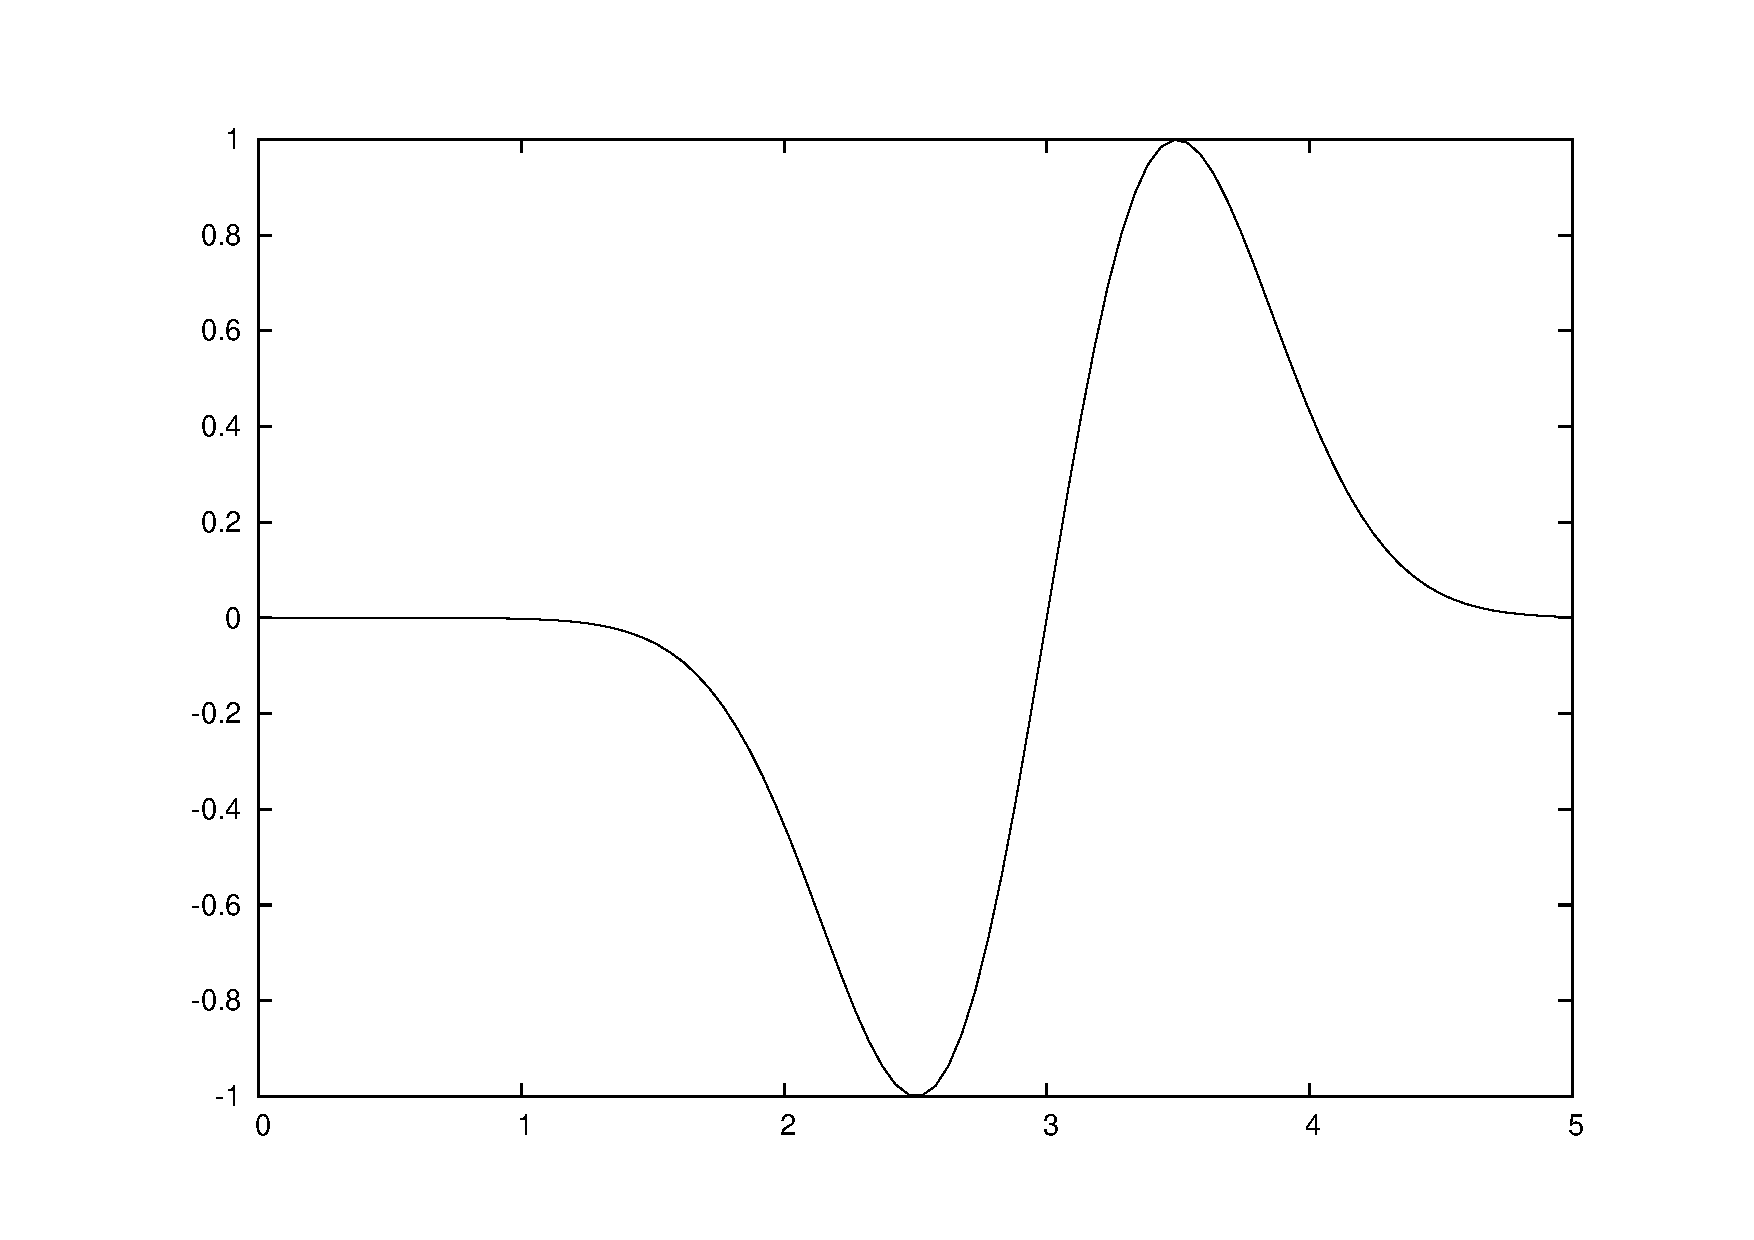
\includegraphics[angle=-90,width=4.in]{figures/waveu}}
\caption{Input Displacement at Source Point ($\alpha=0.7$, $t\hackscore{0}=3$, $U\hackscore{0}=1$).}
\label{WAVE FIG 1.2}
\end{figure}

\begin{figure}[t!]
\centerline{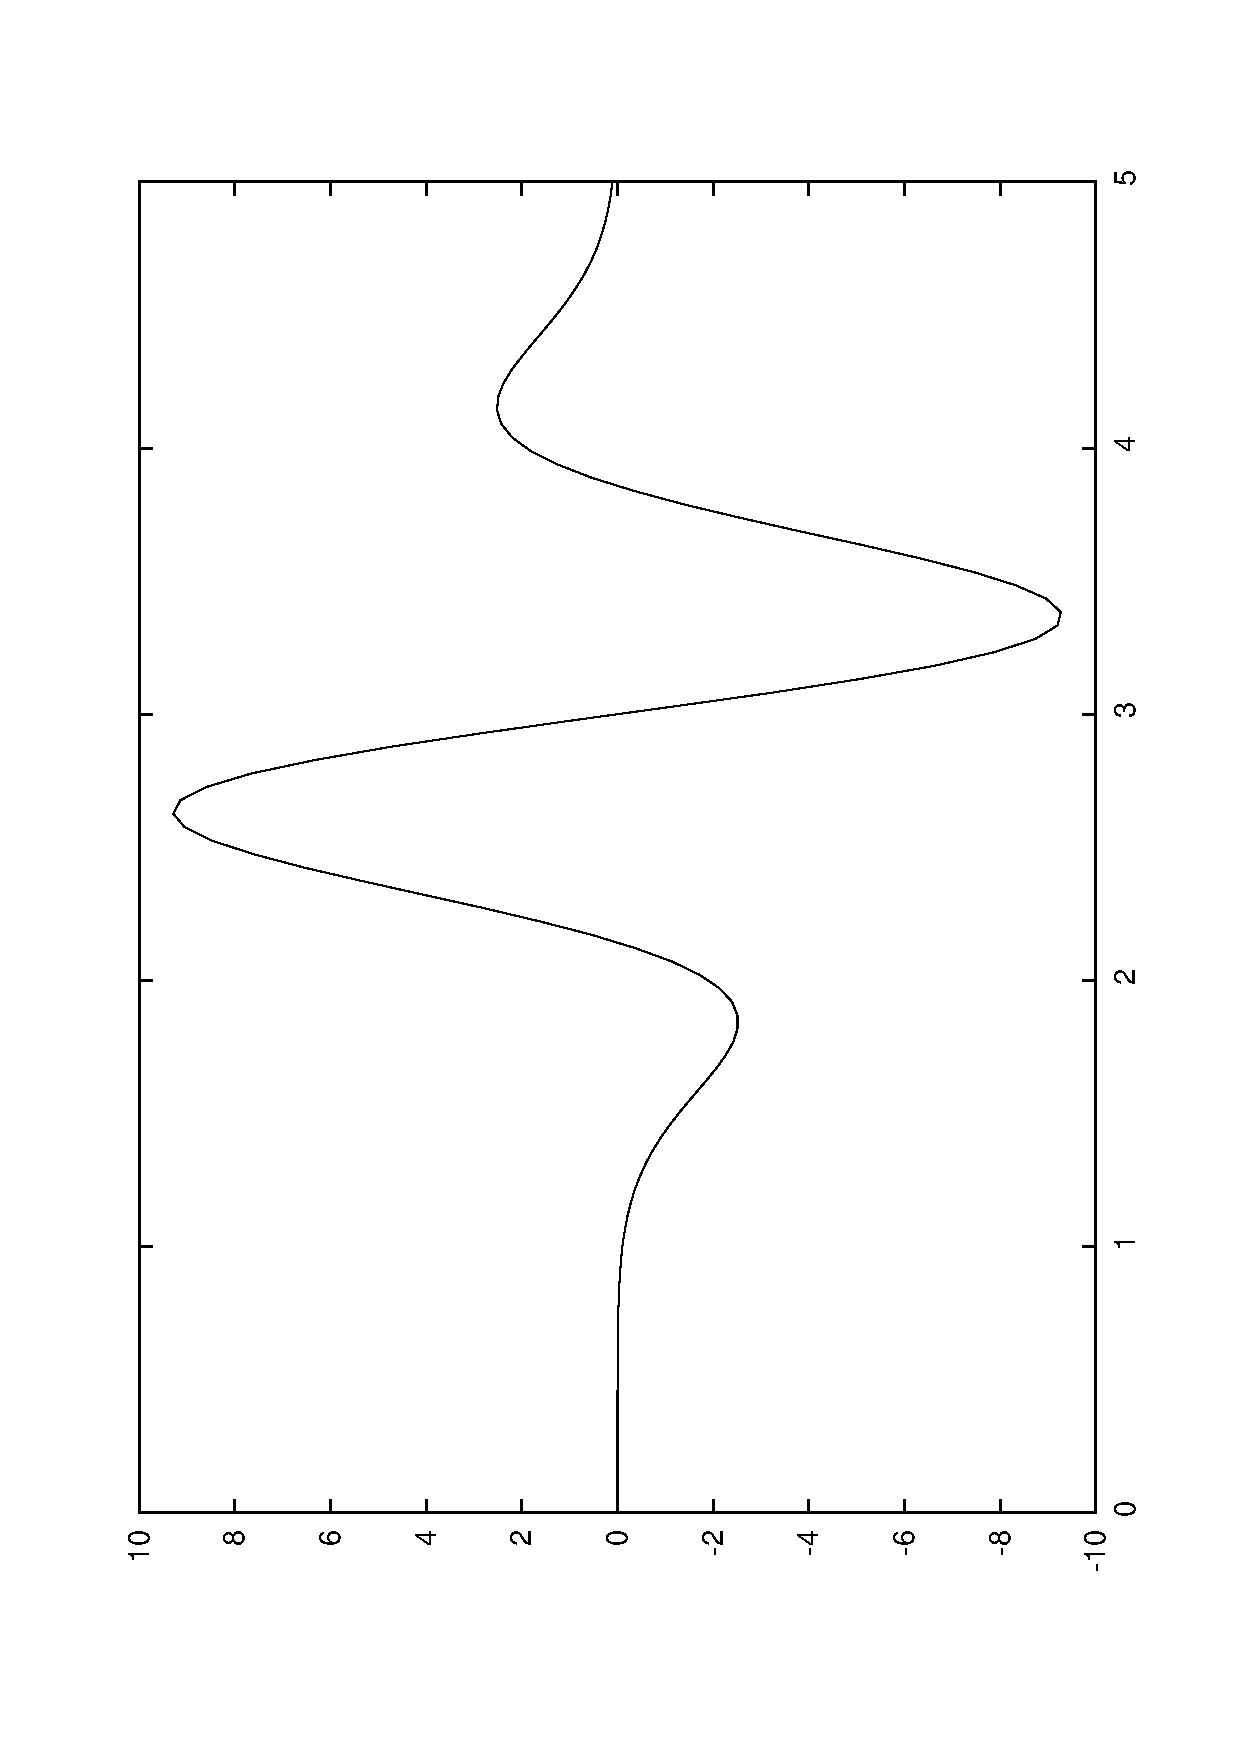
\includegraphics[angle=-90,width=4.in]{figures/wavea}}
\caption{Input Acceleration at Source Point ($\alpha=0.7$, $t\hackscore{0}=3$, $U\hackscore{0}=1$).}
\label{WAVE FIG 1.1}
\end{figure}

Here we are modelling a point source at the point $x\hackscore C$ in the $x\hackscore{0}$-direction
which is a negative puls of amplitude $U\hackscore{0}$ followd by the same 
positive puls. In mathematical terms we use
\begin{eqnarray} \label{WAVE source}
u\hackscore{0}(x\hackscore C,t)= U\hackscore{0} \; \sqrt{2}  \frac{(t-t\hackscore{0})}{\alpha} e^{\frac{1}{2}-\frac{(t-t\hackscore{0})^2}{\alpha^2}} \ 
\end{eqnarray}
for all $t\ge0$ where $\alpha$ is the width of the puls and $t\hackscore{0}$ is the time when
the puls changes from negative to positive. In the simulations we will choose $\alpha=0.3$ and $t\hackscore{0}=2$, see Figure~\ref{WAVE FIG 1.2}
and will apply the source as a constraint in a in a sphere of small radius around the point
$x\hackscore C$.  

 We use an explicit time integration scheme to calculate the displacement field $u$ at 
certain time marks $t^{(n)}$ where $t^{(n)}=t^{(n-1)}+h$ with time step size $h>0$. In the following the upper index ${(n)}$ refers to values at time $t^{(n)}$. We use the Verlet scheme \index{Verlet scheme} with constant time step size $h$
which is defined by
\begin{eqnarray} \label{WAVE dyn 2}
u^{(n)}=2u^{(n-1)}-u^{(n-2)} + h^2 a^{(n)} \\
\end{eqnarray}
for all $n=2,3,\ldots$. It is designed to solve a system of equations of the form
\begin{eqnarray} \label{WAVE dyn 2b} 
u\hackscore{,tt}=G(u)
\end{eqnarray}
where one sets $a^{(n)}=G(u^{(n-1)})$.

In our case $a^{(n)}$ is given by
\begin{eqnarray}\label{WAVE dyn 3}
\rho a^{(n)}\hackscore{i}=\sigma^{(n-1)}\hackscore{ij,j}
\end{eqnarray}
and boundary conditions
\begin{eqnarray} \label{WAVE natural at n}
\sigma^{(n-1)}\hackscore{ij}n\hackscore{j}=0
\end{eqnarray}
derived from \eqn{WAVE natural} where 
\begin{eqnarray} \label{WAVE dyn 3a}
\sigma\hackscore{ij}^{(n-1)} & = & \lambda u^{(n-1)}\hackscore{k,k} \delta\hackscore{ij} + \mu ( u^{(n-1)}\hackscore{i,j} + u^{(n-1)}\hackscore{j,i}).
\end{eqnarray}
We also need to apply the constraint 
\begin{eqnarray} \label{WAVE dyn 3aa}
a^{(n)}\hackscore{0}(x\hackscore C,t)= U\hackscore{0} 
\frac{\sqrt(2.)}{\alpha^2} (4\frac{(t-t\hackscore{0})^3}{\alpha^3}-6\frac{t-t\hackscore{0}}{\alpha})e^{\frac{1}{2}-\frac{(t-t\hackscore{0})^2}{\alpha^2}}
\end{eqnarray}
which is derived from equation~\ref{WAVE source} by calculating the second order time derivative,
see Figure~\ref{WAVE FIG 1.1}. Now we have converted our problem for displacement, $u^{(n)}$, into a problem for 
acceleration, $a^{(n)}$, which now depends 
on the solution at the previous two time steps, $u^{(n-1)}$  and $u^{(n-2)}$.

In each time step we have to solve this problem to get the acceleration $a^{(n)}$, and we will
use the \LinearPDE class of the \linearPDEs to do so. The general form of the PDE defined through
the \LinearPDE class is discussed in \Sec{SEC LinearPDE}. The form which is relevant here is
\begin{equation}\label{WAVE dyn 100}
D\hackscore{ij} a^{(n)}\hackscore{j} = - X\hackscore{ij,j}\; .
\end{equation}
The natural boundary condition
\begin{equation}\label{WAVE dyn 101}
n\hackscore{j}X\hackscore{ij} =0 
\end{equation}
is used. 
With $u=a^{(n)}$ we can identify the values to be assigned to $D$ and $X$:
\begin{equation}\label{WAVE  dyn 6}
\begin{array}{ll}
D\hackscore{ij}=\rho \delta\hackscore{ij}&
X\hackscore{ij}=-\sigma^{(n-1)}\hackscore{ij} \\
\end{array}
\end{equation}
Moreover we need to define the location $r$ where the constraint~\ref{WAVE dyn 3aa} is applied. We will apply
the constraint on a small sphere of radius $R$ around $x\hackscore C$ (we will use 3p.c. of the width of the domain):  
\begin{equation}\label{WAVE  dyn 6 1}
q\hackscore{i}(x) = 
\left\{
\begin{array}{rc}
1 & \|x-x_c\|\le R \\
0 & \mbox{otherwise}
\end{array}
\right.
\end{equation}
The following script defines a the function \function{wavePropagation} which
implements the Verlet scheme to solve our wave propagation problem. 
The argument \var{domain} which is a \Domain class object
defines the domain of the problem. \var{h} and \var{tend} are the time step size
and the end time of the simulation. \var{lam}, \var{mu} and 
\var{rho} are material properties. 
\begin{python}
def wavePropagation(domain,h,tend,lam,mu,rho, x_c, src_radius, U0):
   x=domain.getX()
   # ... open new PDE ...
   mypde=LinearPDE(domain)
   mypde.getSolverOptions().setSolverMethod(mypde.getSolverOptions().LUMPING)
   kronecker=identity(mypde.getDim())



   dunit=numpy.array([1.,0.,0.]) # defines direction of point source

   mypde.setValue(D=kronecker*rho, q=whereNegative(length(x-xc)-src_radius)*dunit)
   # ... set initial values ....
   n=0
   # for first two time steps
   u=Vector(0.,Solution(domain))
   u_last=Vector(0.,Solution(domain))
   t=0

   # define the location of the point source 
   L=Locator(domain,xc)
   # find potential at point source
   u_pc=L.getValue(u)
   print "u at point charge=",u_pc
   # open file to save displacement at point source
   u_pc_data=FileWriter('./data/U_pc.out')
   u_pc_data.write("%f %f %f %f\n"%(t,u_pc[0],u_pc[1],u_pc[2]))

   while t<tend:
     t+=h
     # ... get current stress ....
     g=grad(u)
     stress=lam*trace(g)*kronecker+mu*(g+transpose(g))
     # ... get new acceleration ....
     amplitude=U0*(4*(t-t0)**3/alpha**3-6*(t-t0)/alpha)*sqrt(2.)/alpha**2*exp(1./2.-(t-t0)**2/alpha**2)
     mypde.setValue(X=-stress, r=dunit*amplitude)
     a=mypde.getSolution()
     # ... get new displacement ...
     u_new=2*u-u_last+h**2*a
     # ... shift displacements ....
     u_last=u
     u=u_new
     n+=1
     print n,"-th time step t ",t
     u_pc=L.getValue(u)
     print "u at point charge=",u_pc
     # save displacements at point source to file for t > 0
     u_pc_data.write("%f %f %f %f\n"%(t,u_pc[0],u_pc[1],u_pc[2]))

     # ... save current acceleration in units of gravity and displacements 
     if n==1 or n%10==0: saveVTK("./data/usoln.%i.vtu"%(n/10),acceleration=length(a)/9.81,
     displacement = length(u), tensor = stress, Ux = u[0] )

   u_pc_data.close()
\end{python}
Notice that 
all coefficients of the PDE which are independent of time $t$ are set outside the \code{while} 
loop. This is very efficient since it allows the \LinearPDE class to reuse information as much as possible 
when iterating over time. 

The statement 
\begin{python}
mypde.getSolverOptions().setSolverMethod(mypde.getSolverOptions().LUMPING) 
\end{python}
switches on the use of an aggressive approximation of the PDE operator as a diagonal matrix
formed from the coefficient \var{D}.
The approximation allows, at the cost of 
additional error, very fast 
solution of the PDE. When using lumping the presence of \var{A}, \var{B} or \var{C} will produce wrong results.
 
There are a few new \escript functions in this example: 
\code{grad(u)} returns the gradient $u\hackscore{i,j}$ of $u$ (in fact \var{grad(g)[i,j]}=$=u\hackscore{i,j}$).
There are restrictions on the argument of the \function{grad} function, for instance
the statement \code{grad(grad(u))} will raise an exception.
\code{trace(g)} returns the sum of the main diagonal elements \var{g[k,k]} of \var{g} 
and \code{transpose(g)} returns the matrix transpose of \var{g} (ie. $\var{transpose(g)[i,j]}=\var{g[j,i]}$). 

We initialize the values of \code{u} and \code{u_last} to be zero. It is important
to initialize both with the \SolutionFS \FunctionSpace as they have to be seen as solutions of PDEs from previous time steps. In fact, the \function{grad} does not accept arguments with a certain \FunctionSpace, for more details see \Sec{SEC ESCRIPT DATA}. 

The \class{Locator} is designed to extract values at a given location (in this case $x\hackscore C$) from functions such as the displacement vector \code{u}. Typically the \class{Locator} is used in the following form:  
\begin{python}
L=Locator(domain,xc)
u=...
u_pc=L.getValue(u)
\end{python}
The return value \code{u_pc} is the value of \code{u} at the location \code{xc}\footnote{In fact the finite element node which is closest to the given position. The usage of  \class{Locator} is MPI save.}.


The output \code{U_pc.out} and \code{vtu} files are saved in a directory called \code{data}.
The \code{U_pc.out} stores 4 columns of data: $t,u\hackscore x,u\hackscore y,u\hackscore z$ 
respectively, where $u\hackscore x,u\hackscore y,u\hackscore z$ are the $x\hackscore 0,x\hackscore 1,x\hackscore 2$ components of 
the displacement vector $u$ at the point source. These can be
plotted easily using any plotting package. In gnuplot the command:
\begin{verbatim}
 plot 'U_pc.out' u 1:2 title 'U_x' w l lw 2, 'U_pc.out' u 1:3 title 'U_y' w l lw 2, 
'U_pc.out' u 1:4 title 'U_z' w l lw 2
\end{verbatim}
will reproduce Figure~\ref{WAVE FIG 1} (As expected this is identical to the input signal shown in Figure~\ref{WAVE FIG 1.2})2. It is pointed out that we are not using the
standart \PYTHON \function{open} to create the file \code{U_pc.out} as it is not 
when running \escript under MPI, see chapter~\ref{EXECUTION} for more details.

One of the big advantages of the Verlet scheme is the fact that the problem to be solved 
in each time step is very simple and does not involve any spatial derivatives (which is what allows us to use lumping in this simulation).
The problem becomes so simple because we use the stress from the last time step rather then the stress which is
actually present at the current time step. Schemes using this approach are called an explicit time integration 
schemes \index{explicit scheme} \index{time integration!explicit}. The 
backward Euler scheme we have used in \Chap{DIFFUSION CHAP} is 
an example of an implicit scheme
\index{implicit scheme} \index{time integration!implicit}. In this case one uses the actual status of 
each variable at a particular time rather then values from previous time steps. This will lead to a problem which is 
more expensive to solve, in particular for non-linear problems. 
Although 
explicit time integration schemes are cheap to finalize a single time step, they need significantly smaller time
steps then implicit schemes and can suffer from stability problems. Therefore they need a 
very careful selection of the time step size $h$.

An easy, heuristic way of choosing an appropriate
time step size is the Courant condition \index{Courant condition} \index{explicit scheme!Courant condition}
which says that within a time step a information should not travel further than a cell used in the 
discretization scheme. In the case of the wave equation the velocity of a (p-) wave is given as
$\sqrt{\frac{\lambda+2\mu}{\rho}}$ so one should choose $h$ from
\begin{eqnarray}\label{WAVE dyn 66}
h= \frac{1}{5} \sqrt{\frac{\rho}{\lambda+2\mu}} \Delta x
\end{eqnarray}
where $\Delta x$ is the cell diameter. The factor $\frac{1}{5}$ is a safety factor considering the heuristics of 
the formula. 

The following script uses the \code{wavePropagation} function to solve the
wave equation for a point source located at the bottom face of a block. The width of the block in 
each direction on the bottom face is $10\mbox{km}$ ($x\hackscore 0$ and $x\hackscore 1$ directions ie. \code{l0} and \code{l1}).
The \code{ne} gives the number of elements in $x\hackscore{0}$ and $x\hackscore 1$ directions.  
The depth of the block is aligned with the $x\hackscore{2}$-direction. 
The depth (\code{l2}) of the block in
the $x\hackscore{2}$-direction is chosen so that there are 10 elements and the magnitude of the
of the depth is chosen such that the elements 
become cubic. We chose 10 for the number of elements in $x\hackscore{2}$-direction so that the 
computation would be faster. \code{Brick($n\hackscore 0,  n\hackscore 1, n\hackscore 2,l\hackscore 0,l\hackscore 1,l\hackscore 2$)} is an \finley function which creates a rectangular mesh 
with $n\hackscore 0 \times n\hackscore 1 \times n\hackscore2$ elements over the brick $[0,l\hackscore 0] \times [0,l\hackscore 1] \times [0,l\hackscore 2]$.
\begin{python}
from esys.finley import Brick
ne=32          # number of cells in x_0 and x_1 directions
width=10000.  # length in x_0 and x_1 directions
lam=3.462e9
mu=3.462e9
rho=1154.
tend=60
U0=1. # amplitude of point source
# spherical source at middle of bottom face
xc=[width/2.,width/2.,0.]
# define small radius around point xc
src_radius = 0.03*width
print "src_radius = ",src_radius

mydomain=Brick(ne,ne,10,l0=width,l1=width,l2=10.*width/32.)
h=(1./5.)*inf(sqrt(rho/(lam+2*mu))*inf(domain.getSize())
print "time step size = ",h
wavePropagation(mydomain,h,tend,lam,mu,rho,xc, src_radius, U0)
\end{python}
The \function{domain.getSize()} return the local element size $\Delta x$. The 
\function{inf} makes sure that the Courant condition~\ref{WAVE dyn 66} olds everywhere in the domain. 

The script is available as \file{wave.py} in the \ExampleDirectory \index{scripts!\file{wave.py}}. 
To visualize the results from the data directory: 
\begin{verbatim} mayavi -d usoln.1.vtu -m SurfaceMap &\end{verbatim} You can rotate this figure by clicking on it with the mouse and moving it around.
Again use \code{Configure Data} to move backwards and forward in time, and 
also to choose the results (acceleration, displacement or $u\hackscore x$) by using \code{Select Scalar}. Figure \ref{WAVE FIG 2} shows the results for the displacement at various time steps.

\begin{figure}[t!]
\centerline{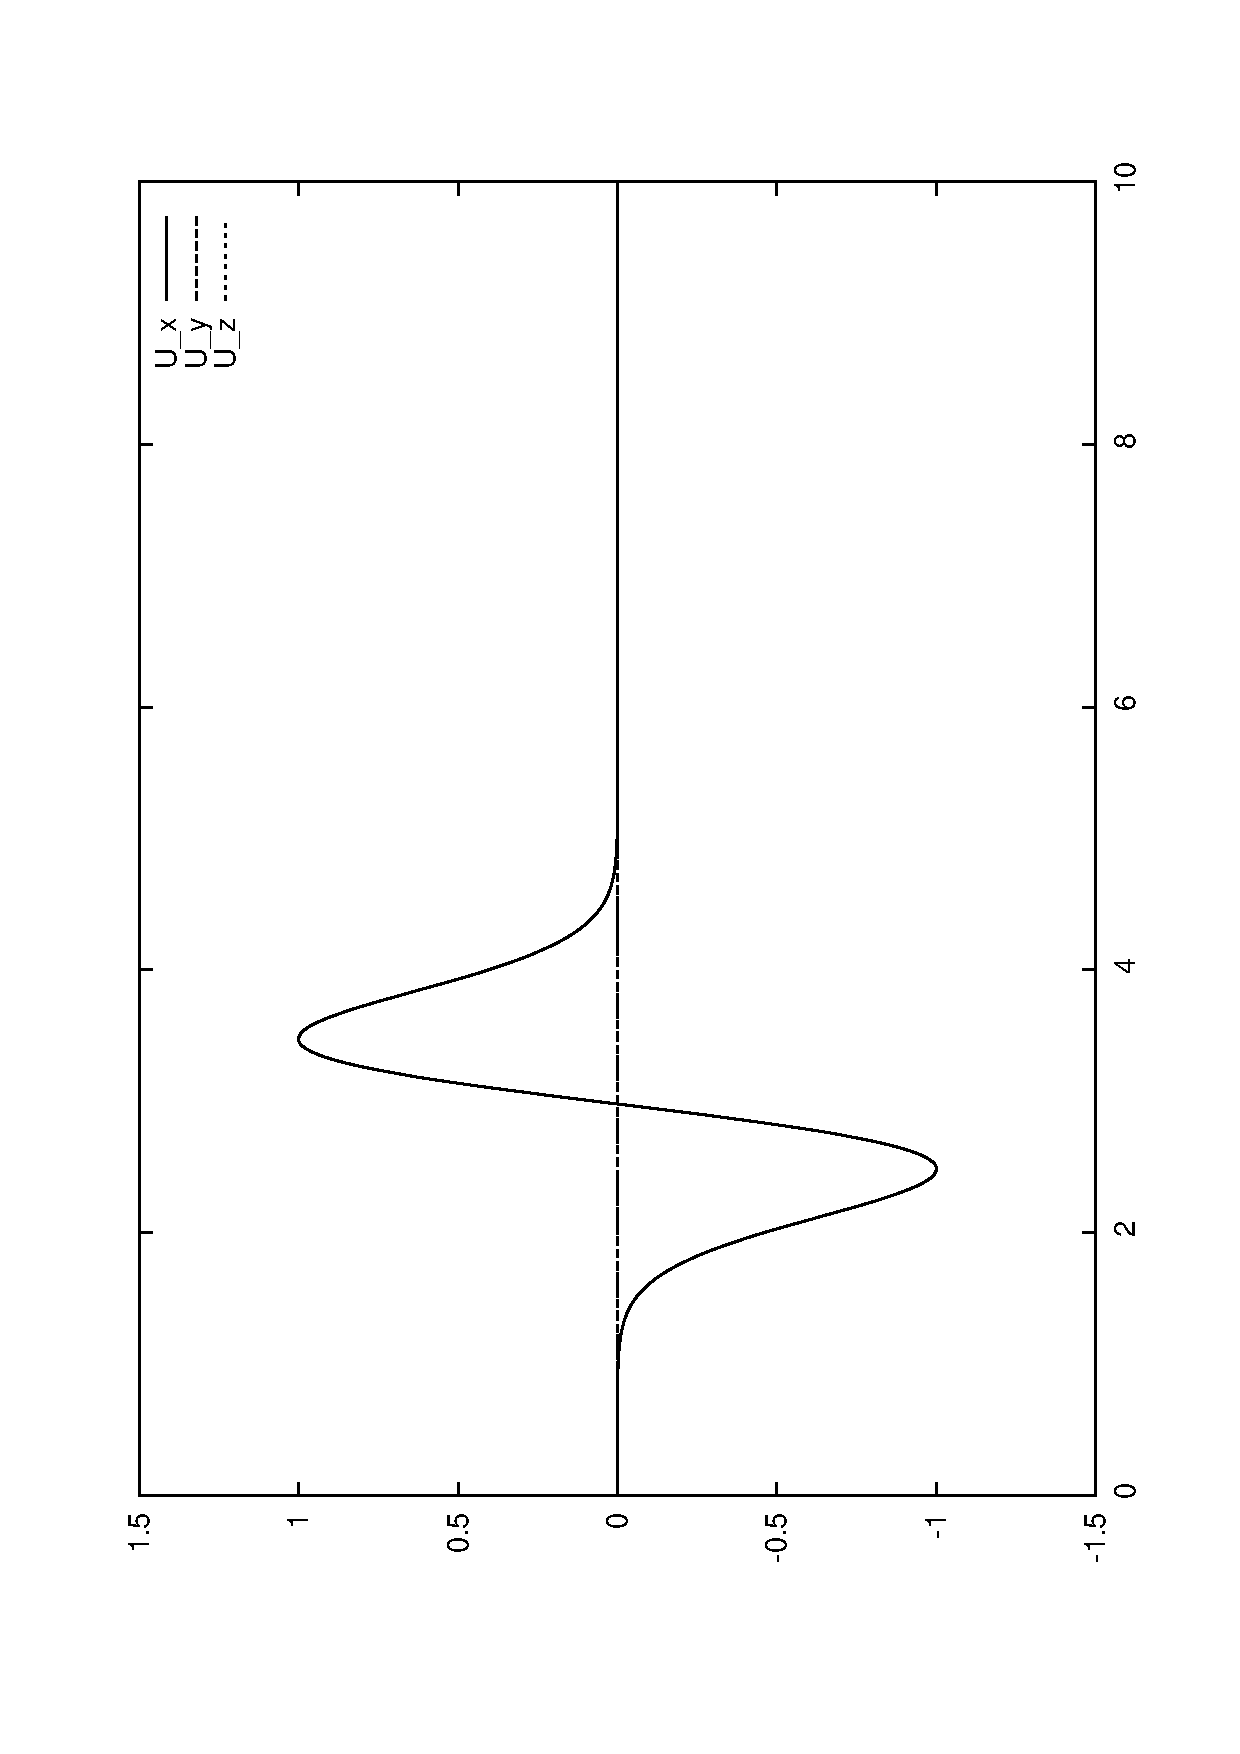
\includegraphics[width=4.in, angle=-90]{figures/WavePC}}
\caption{Amplitude at Point source from the Simulation.}
\label{WAVE FIG 1}
\end{figure}

\begin{figure}[t]
\begin{center}
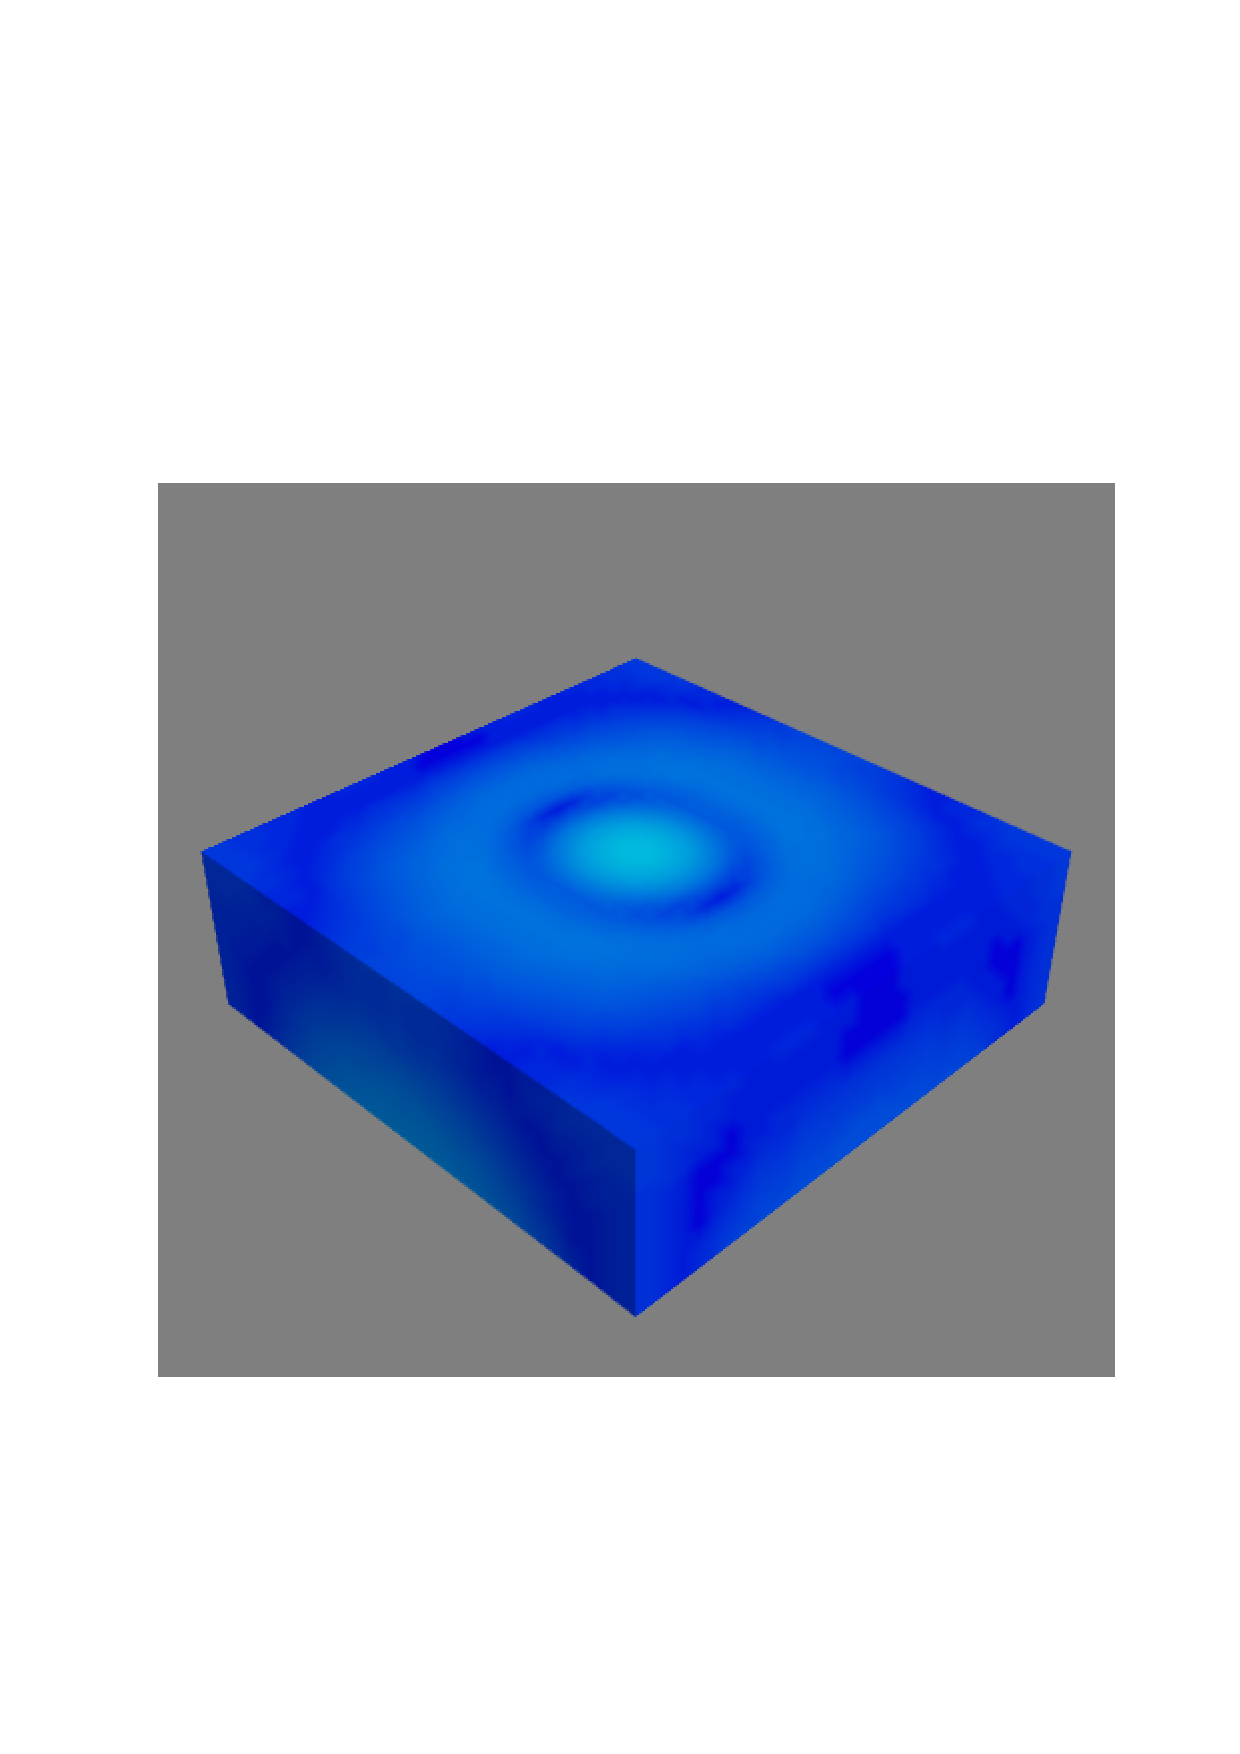
\includegraphics[width=2in]{figures/Wave11}
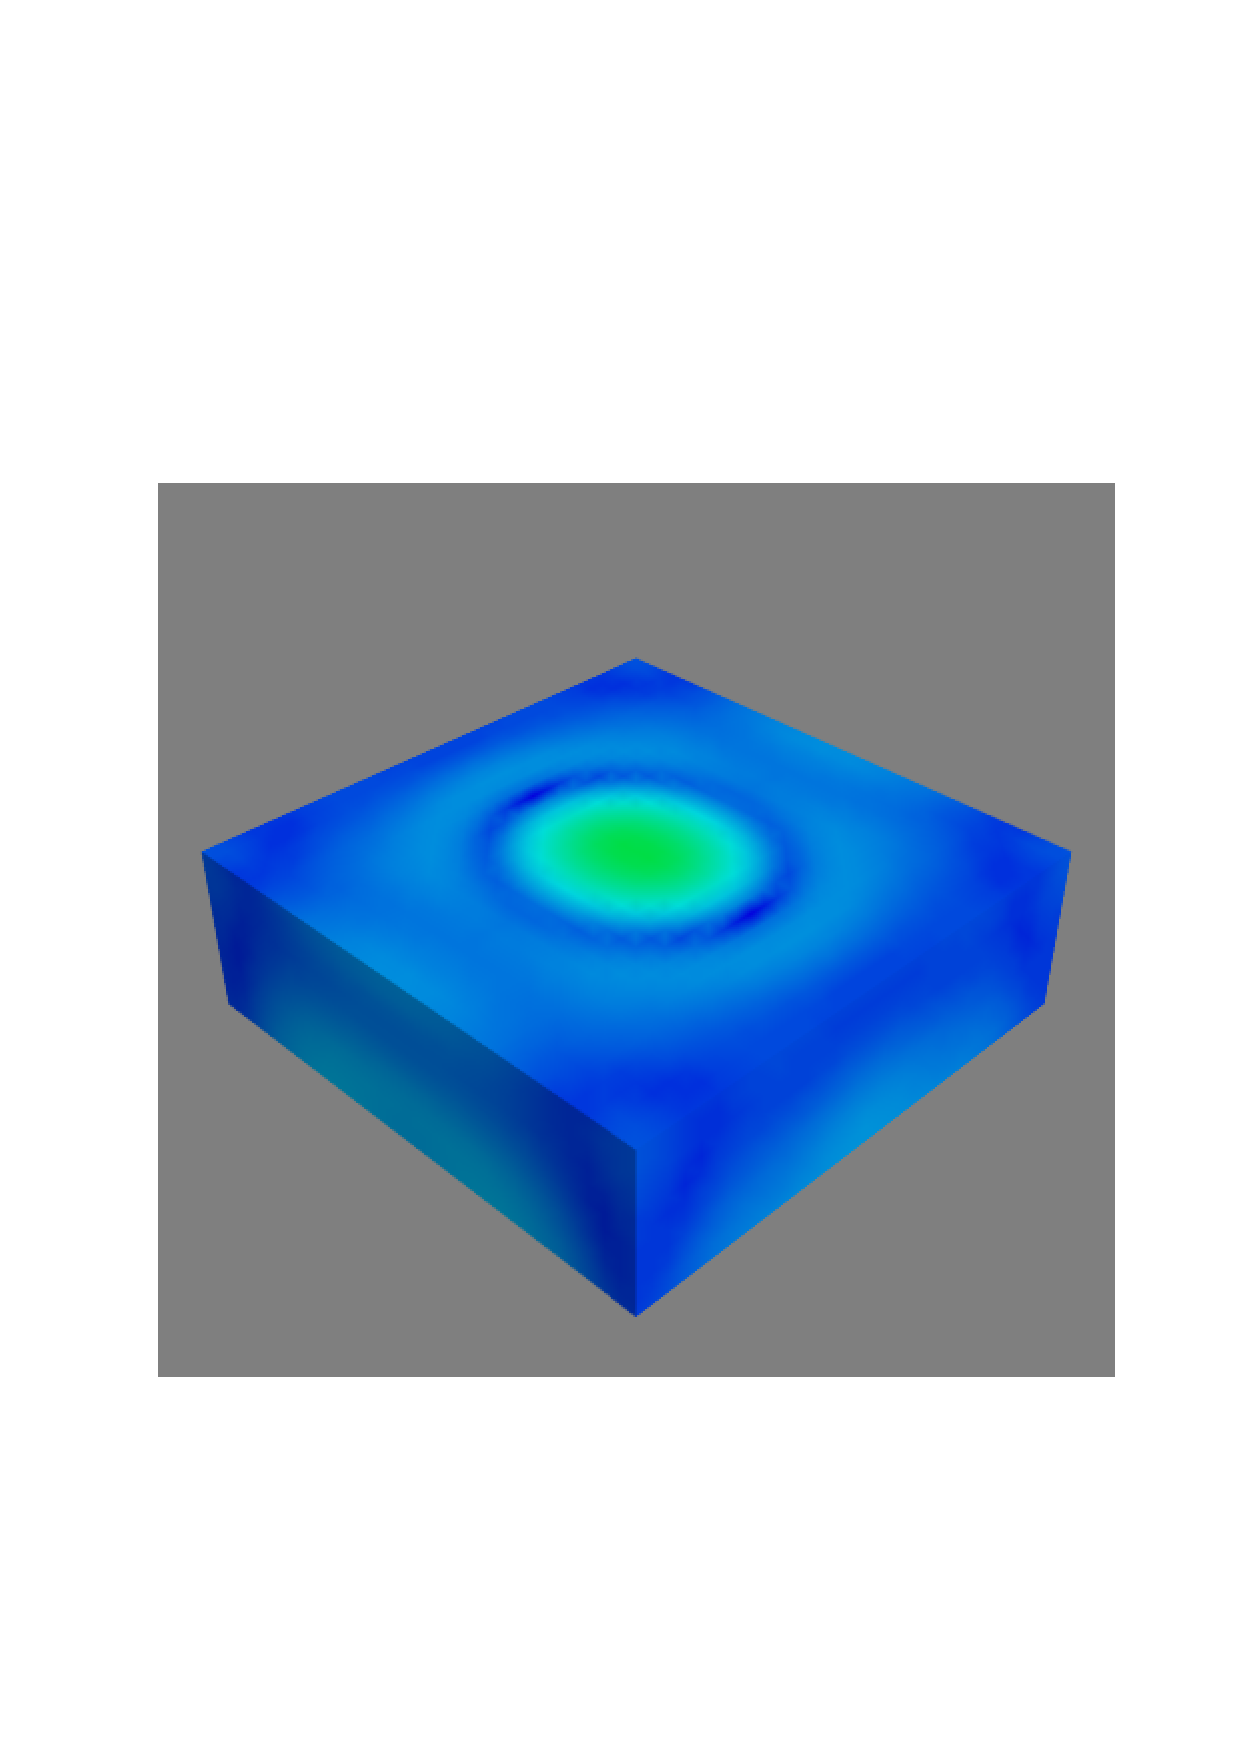
\includegraphics[width=2in]{figures/Wave22}
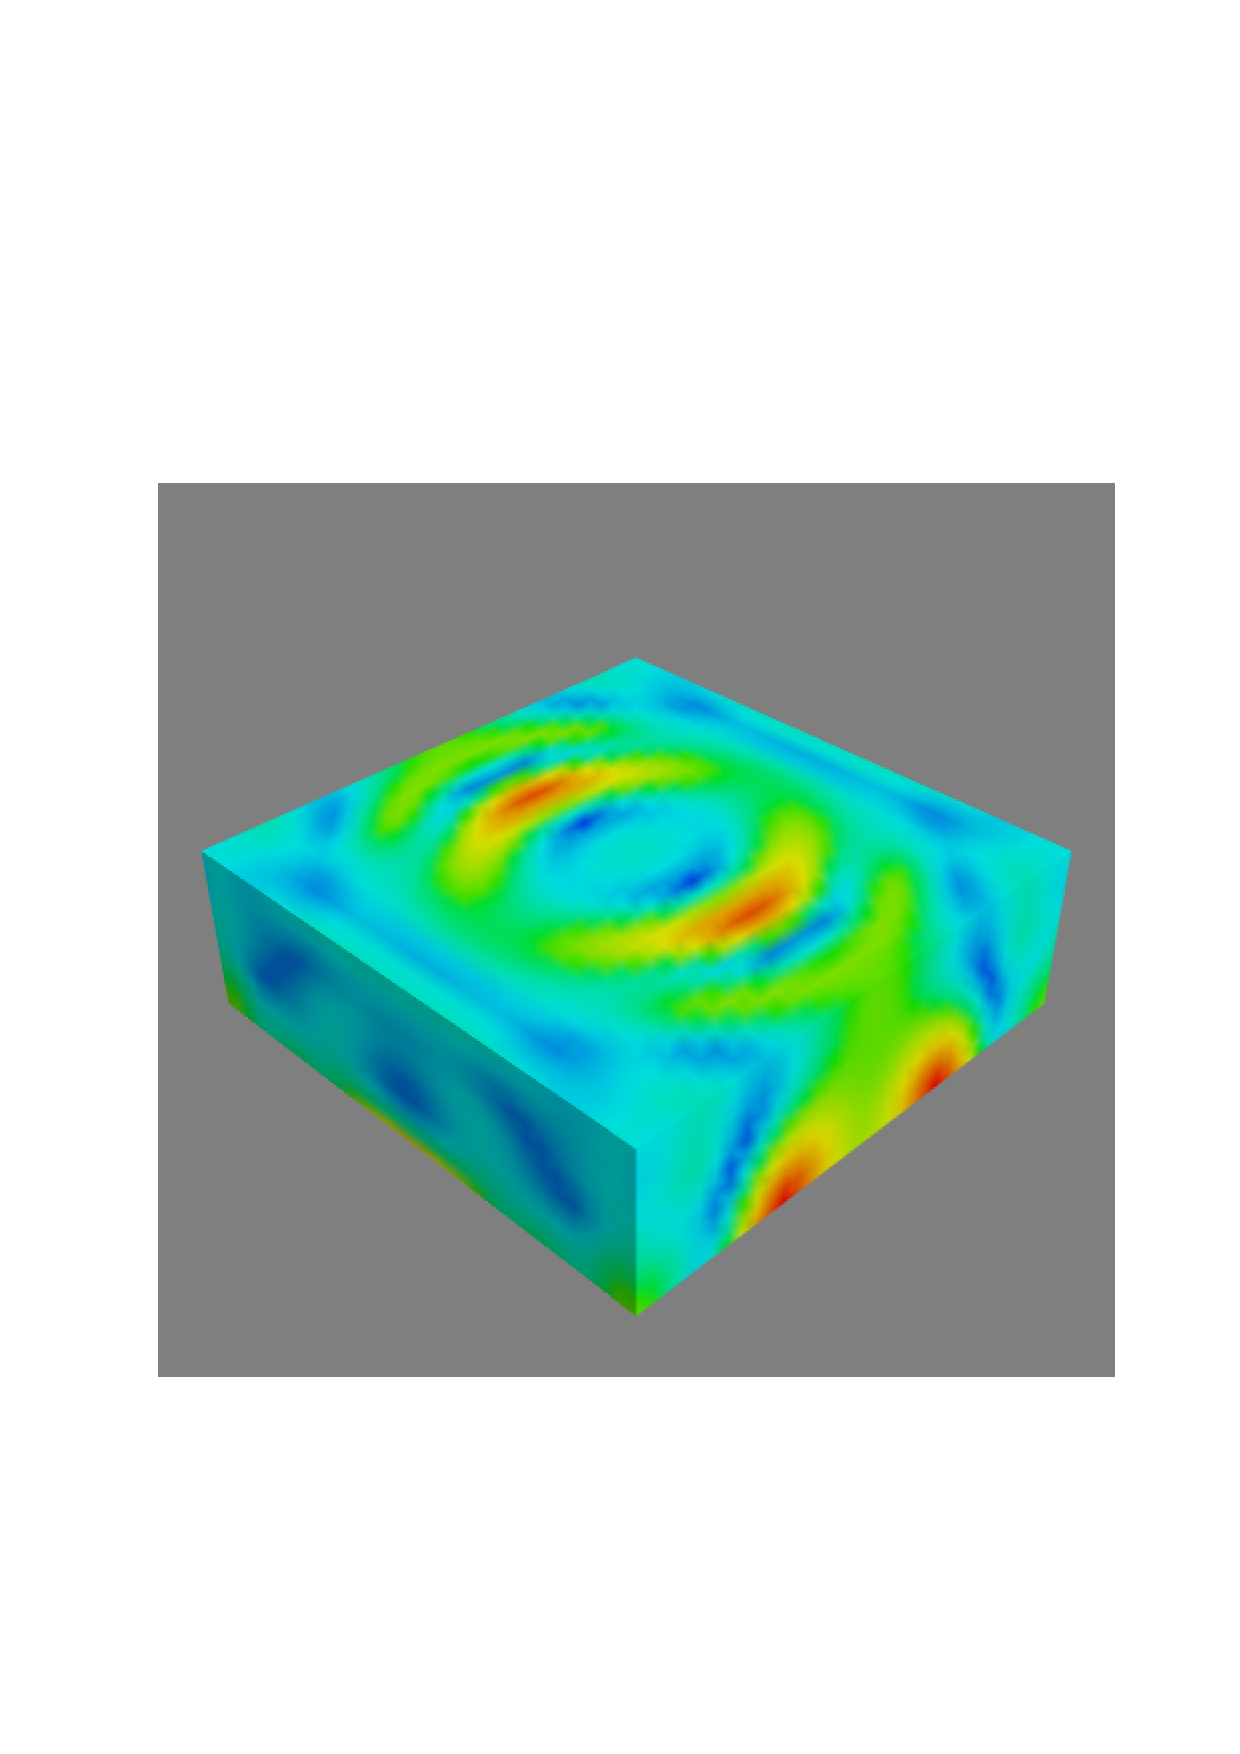
\includegraphics[width=2in]{figures/Wave28}
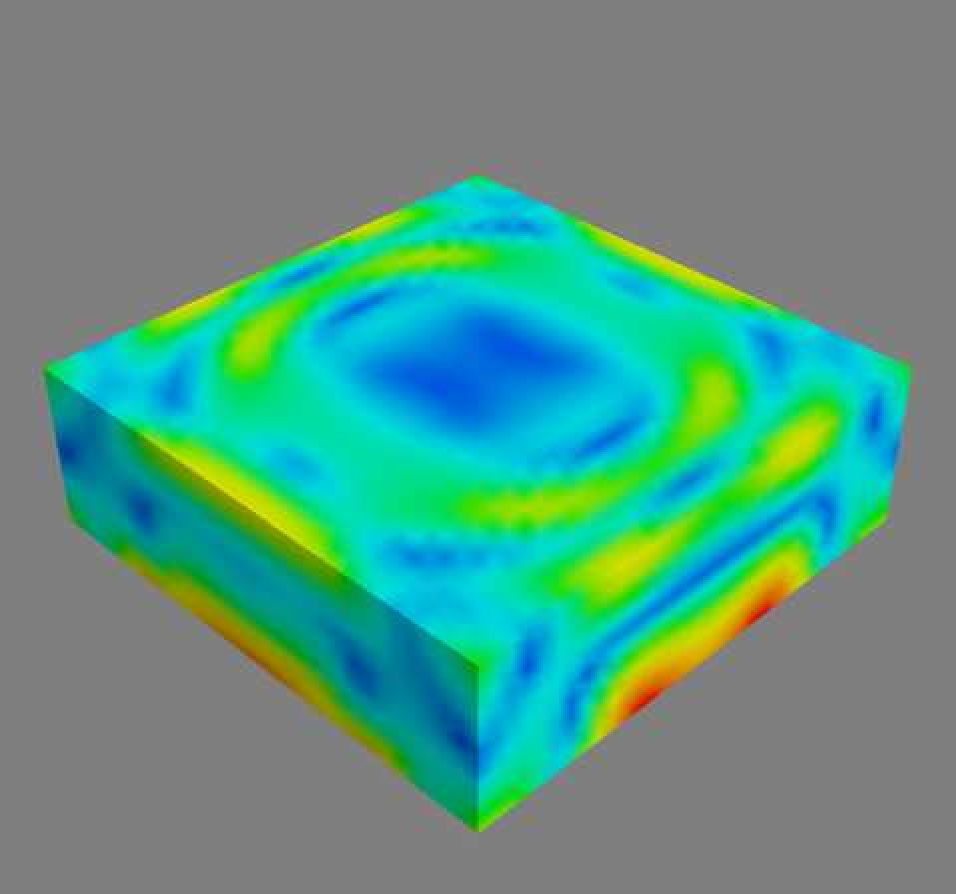
\includegraphics[width=2in]{figures/Wave32}
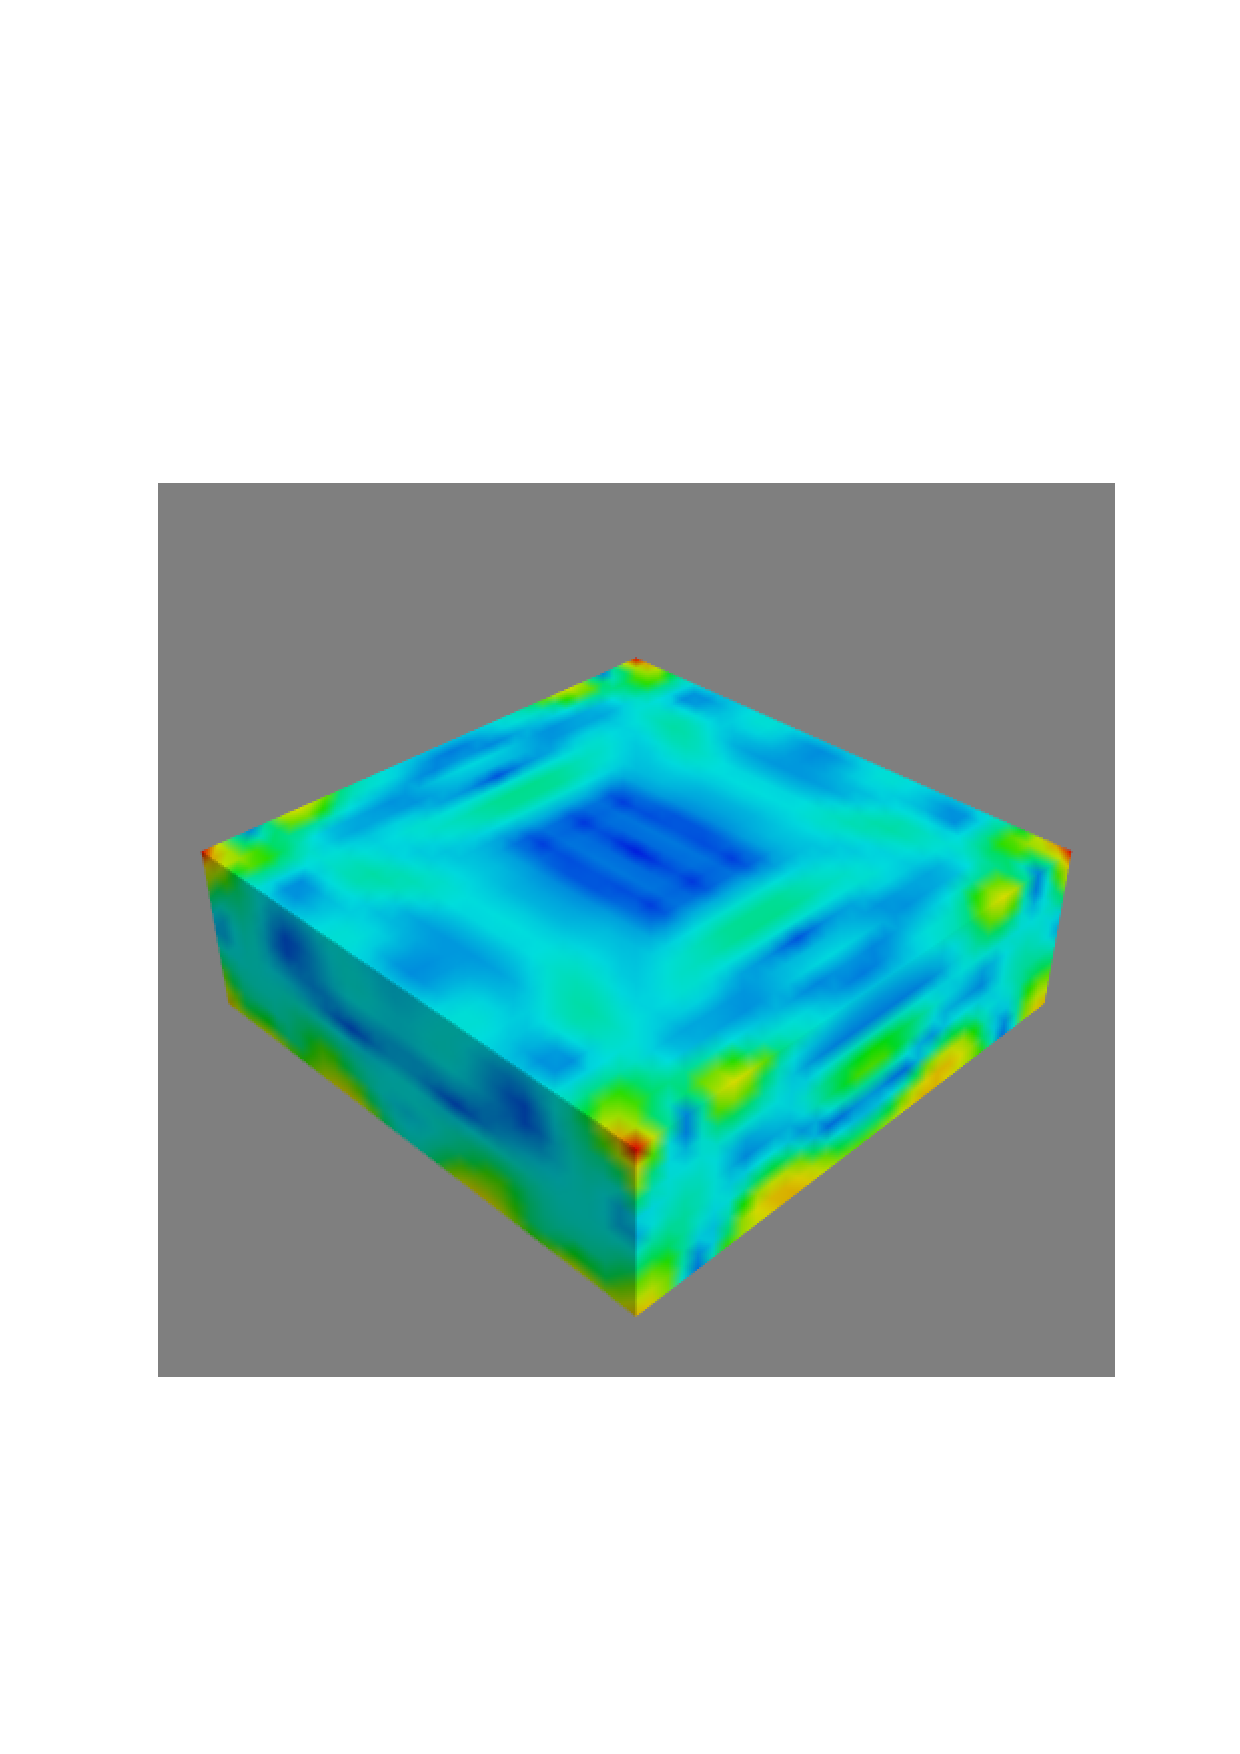
\includegraphics[width=2in]{figures/Wave36}
\end{center}
\caption{Selected time steps ($n = 11, 22, 32, 36$) of a wave propagation over a $10\mbox{km} \times 10\mbox{km} \times 3.125\mbox{km}$ block 
from a point source initially at $(5\mbox{km},5\mbox{km},0)$
with time step size $h=0.02083$. Color represents the displacement.
Here the view is oriented onto the bottom face.
\label{WAVE FIG 2}}
\end{figure}


%%%%%%%%%%%%%%%%%%%%%%%%%%%%%%%%%%%%%%%%%%%%%%%%%%%%%%%%
%
% Copyright (c) 2003-2008 by University of Queensland
% Earth Systems Science Computational Center (ESSCC)
% http://www.uq.edu.au/esscc
%
% Primary Business: Queensland, Australia
% Licensed under the Open Software License version 3.0
% http://www.opensource.org/licenses/osl-3.0.php
%
%%%%%%%%%%%%%%%%%%%%%%%%%%%%%%%%%%%%%%%%%%%%%%%%%%%%%%%%


\section{Elastic Deformation}
\label{ELASTIC CHAP}
In this section we want to examine the deformation of a linear elastic body caused by expansion through a heat distribution. We want 
a displacement field $u\hackscore{i}$ which solves the momentum equation
\index{momentum equation}:
\begin{eqnarray}\label{HEATEDBLOCK general problem}
 - \sigma\hackscore{ij,j}=0
\end{eqnarray}
where the stress $\sigma$ is given by
\begin{eqnarray}\label{HEATEDBLOCK linear elastic}
 \sigma\hackscore{ij}= \lambda u\hackscore{k,k} \delta\hackscore{ij} + \mu ( u\hackscore{i,j} + u\hackscore{j,i})
 - (\lambda+\frac{2}{3} \mu)  \; \alpha  \;  (T-T\hackscore{ref})\delta\hackscore{ij} \;.
\end{eqnarray}
In this formula $\lambda$ and $\mu$ are the Lame coefficients, $\alpha$ is the 
temperature expansion coefficient, $T$ is the temperature distribution and $T_{ref}$ a reference temperature. Note that 
\eqn{HEATEDBLOCK general problem} is similar to eqn{WAVE general problem} introduced in section~\Sec{WAVE CHAP} but the
inertia term $\rho u\hackscore{i,tt}$ has been dropped as we assume a static scenario here. Moreover, in 
comparison to the \eqn{WAVE stress}
definition of stress $\sigma$ in \eqn{HEATEDBLOCK linear elastic} an extra term is introduced 
to bring in stress due to volume changes trough temperature dependent expansion.   

Our domain is the unit cube 
\begin{eqnarray} \label{HEATEDBLOCK natural location}
\Omega=\{(x\hackscore{i} | 0 \le x\hackscore{i} \le 1 \}
\end{eqnarray}
On the boundary the normal stress component is set to zero
\begin{eqnarray} \label{HEATEDBLOCK natural}
\sigma\hackscore{ij}n\hackscore{j}=0
\end{eqnarray}
and on the face with $x\hackscore{i}=0$ we set the $i$-th component of the displacement to $0$
\begin{eqnarray} \label{HEATEDBLOCK constraint}
u\hackscore{i}(x)=0 & \mbox{ where } & x\hackscore{i}=0 \; 
\end{eqnarray}
For the temperature distribution we use 
\begin{eqnarray} \label{HEATEDBLOCK temperature}
T(x)= T\hackscore{0} e^{-\beta \|x-x^{c}\|}; 
\end{eqnarray}
with a given positive constant $\beta$ and location $x^{c}$ in the domain. 

%Later in \Sec{MODELFRAME} we will use
% $T$ from a time-dependent temperature diffusion problem as discussed in \Sec{DIFFUSION CHAP}.

When we insert~\eqn{HEATEDBLOCK linear elastic} we get a second order system of linear PDEs for the displacements $u$ which is called
the Lame equation\index{Lame equation}. We want to solve
this using the \LinearPDE class to this. For a system of PDEs and a solution with several components the \LinearPDE class 
takes PDEs of the form
\begin{equation}\label{LINEARPDE.SYSTEM.1 TUTORIAL}
-(A\hackscore{ijkl} u\hackscore{k,l})\hackscore{,j}=-X\hackscore{ij,j} \; .
\end{equation}
$A$ is of \RankFour and $X$ is of \RankTwo. We show here the coefficients relevant 
for the we trying to solve. The full form is given in~\eqn{LINEARPDE.SYSTEM.1}. 
The natural boundary conditions \index{boundary condition!natural} take the form:
\begin{equation}\label{LINEARPDE.SYSTEM.2 TUTORIAL}
n\hackscore{j} A\hackscore{ijkl} u\hackscore{k,l}=n\hackscore{j}X\hackscore{ij} \;.
\end{equation}
Constraints \index{constraint} take the form
\begin{equation}\label{LINEARPDE.SYSTEM.3 TUTORIAL}
u\hackscore{i}=r\hackscore{i} \mbox{ where } q\hackscore{i}>0
\end{equation}
$r$ and $q$ are each \RankOne. 
We can easily identify the coefficients in~\eqn{LINEARPDE.SYSTEM.1 TUTORIAL}:
\begin{eqnarray}\label{LINEARPDE ELASTIC COEFFICIENTS}
A\hackscore{ijkl}=\lambda \delta\hackscore{ij} \delta\hackscore{kl} + \mu ( 
\delta\hackscore{ik} \delta\hackscore{jl}
+ \delta\hackscore{il} \delta\hackscore{jk}) \\
X\hackscore{ij}=(\lambda+\frac{2}{3} \mu) \;  \alpha \; (T-T\hackscore{ref})\delta\hackscore{ij} \\
\end{eqnarray}
The characteristic function $q$ defining the locations and components where constraints are set is given by:
\begin{equation}\label{HEATEDBLOCK MASK}
q\hackscore{i}(x)=\left\{ 
\begin{array}{cl}
1  & x\hackscore{i}=0  \\ 
0  & \mbox{otherwise}   \\
\end{array}
\right. 
\end{equation}
Under the assumption that $\lambda$, $\mu$, $\beta$ and $T\hackscore{ref}$ 
are constant we may use $Y\hackscore{i}=\lambda+\frac{2}{3} \mu) \; \alpha \; T\hackscore{i}$. However,
this choice would lead to a different natural boundary condition which does not set the normal stress component as defined
in~\eqn{HEATEDBLOCK linear elastic} to zero.

Analogously to concept of symmetry for a single PDE, we call the PDE defined by~\eqn{LINEARPDE.SYSTEM.1 TUTORIAL} symmetric if
\index{symmetric PDE}
\begin{eqnarray}\label{LINEARPDE.SYSTEM.SYMMETRY TUTORIAL}
A\hackscore{ijkl} =A\hackscore{klij} \\
\end{eqnarray}
This Lame equation is in fact symmetric, given the difference in $D$ and $d$ as compared to the scalar case.
The \LinearPDE class is notified of this fact by calling its \method{setSymmetryOn} method.

After we have solved the Lame equation we want to analyse the actual stress distribution. Typically the von--Mises stress\index{von--Mises stress} defined by
\begin{equation}
\sigma\hackscore{mises} = \sqrt{
\frac{1}{2} ((\sigma\hackscore{00}-\sigma\hackscore{11})^2
            + (\sigma\hackscore{11}-\sigma\hackscore{22})^2
            + (\sigma\hackscore{22}-\sigma\hackscore{00})^2)
+ 3( \sigma\hackscore{01}^2+\sigma\hackscore{12}^2+\sigma\hackscore{20}^2) }
\end{equation}
is used to detect material damage. Here we want to calculate the von--Mises and write the stress to a file for visualization.

\index{scripts!\file{diffusion.py}}
The following script, which is available in \file{heatedbox.py} in the \ExampleDirectory, solves the Lame equation
and writes the displacements and the von--Mises stress\index{von--Mises stress} into a file \file{deform.xml} in the \VTK file format: 
\begin{python}
from esys.escript import *
from esys.escript.linearPDEs import LinearPDE
from esys.finley import Brick
#... set some parameters ...
lam=1.
mu=0.1
alpha=1.e-6
xc=[0.3,0.3,1.]
beta=8.
T_ref=0.
T_0=1.
#... generate domain ...
mydomain = Brick(l0=1.,l1=1., l2=1.,n0=10, n1=10, n2=10)
x=mydomain.getX()
#... set temperature ...
T=T_0*exp(-beta*length(x-xc))
#... open symmetric PDE ...
mypde=LinearPDE(mydomain)
mypde.setSymmetryOn()
#... set coefficients ...
C=Tensor4(0.,Function(mydomain))
for i in range(mydomain.getDim()):
  for j in range(mydomain.getDim()):
     C[i,i,j,j]+=lam
     C[j,i,j,i]+=mu
     C[j,i,i,j]+=mu
msk=whereZero(x[0])*[1.,0.,0.] \
   +whereZero(x[1])*[0.,1.,0.] \
   +whereZero(x[2])*[0.,0.,1.]
sigma0=(lam+2./3.*mu)*alpha*(T-T_ref)*kronecker(mydomain)
mypde.setValue(A=C,X=sigma0,q=msk)
#... solve pde ...
u=mypde.getSolution()
#... calculate von-Misses stress
g=grad(u)
sigma=mu*(g+transpose(g))+lam*trace(g)*kronecker(mydomain)-sigma0
sigma_mises=sqrt(((sigma[0,0]-sigma[1,1])**2+(sigma[1,1]-sigma[2,2])**2+ \
                  (sigma[2,2]-sigma[0,0])**2)/2. \
                 +3*(sigma[0,1]**2 + sigma[1,2]**2 + sigma[2,0]**2))
#... output ...
saveVTK("deform.xml",disp=u,stress=sigma_mises)
\end{python}

\begin{figure}
\centerline{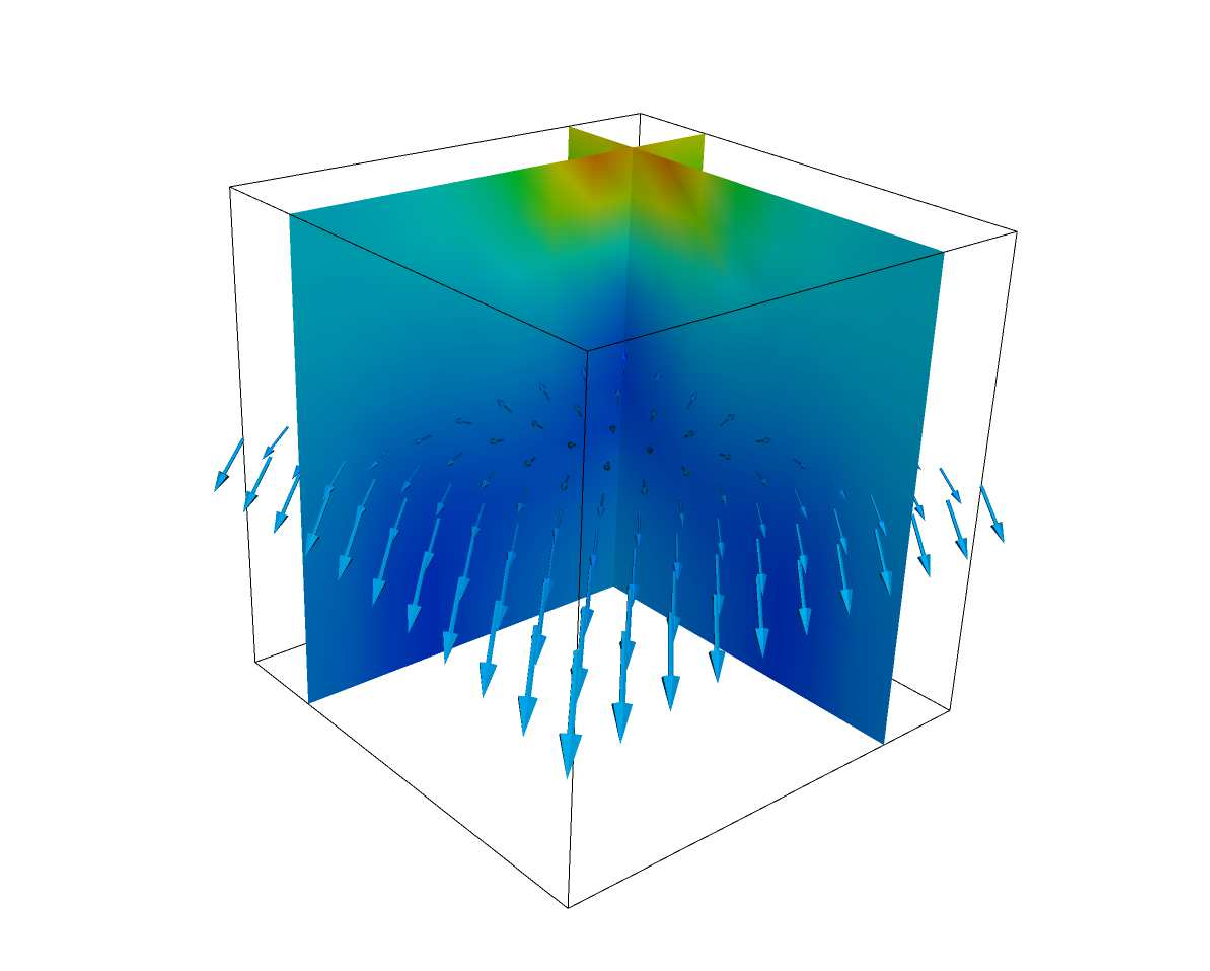
\includegraphics[width=\figwidth]{figures/HeatedBlock}}
\caption{von--Mises Stress and Displacement Vectors.}
\label{HEATEDBLOCK FIG 2}
\end{figure}

Finally the the results can be visualize by calling
\begin{python}
mayavi -d deform.xml -f CellToPointData -m VelocityVector -m SurfaceMap &
\end{python}
Note that the filter \text{CellToPointData} is applied to create smooth representation of the 
von--Mises stress. \fig{HEATEDBLOCK FIG 2} shows the results where the vertical planes showing the 
von--Mises stress and the horizontal plane shows the vector representing displacements.



\section{Stokes Flow}
\label{STOKES FLOW CHAP}

In this section we will look at Computational Fluid Dynamics (CFD) to simulate the flow of fluid under the influence of gravity. The StokesProblemCartesian class will be used to calculate the velocity and pressure of the fluid.
The fluid dynamics is governed by the Stokes equation. In geophysical problems the velocity of fluids are low; that is, the inertial forces are small compared with the viscous forces, therefore the inertial terms in the Navier-Stokes equations can be ignored. For a body force, $f$, the governing equations are given by:
%
\begin{equation}
\nabla \cdot (\eta(\nabla \vec{v} + \nabla^{T} \vec{v})) - \nabla p = -f,
\label{GENERAL NAVIER STOKES}
\end{equation}
%
with the incompressibility condition
%
\begin{equation}
\nabla \cdot \vec{v} = 0.
\label{INCOMPRESSIBILITY}
\end{equation}
%
where $p$, $\eta$ and $f$ are the pressure, viscosity and body forces, respectively. 
Alternatively, the Stokes equations can be represented in Einstein summation tensor notation (compact notation):
%
\begin{equation}
-(\eta(v\hackscore{i,j} + v\hackscore{j,i})),\hackscore{j} - p,\hackscore{i} = f\hackscore{i},
\label{GENERAL NAVIER STOKES COM}
\end{equation}
%
with the incompressibility condition
%
\begin{equation}
-v\hackscore{i,i} = 0.
\label{INCOMPRESSIBILITY COM}
\end{equation}
%
The subscript comma $i$ denotes the derivative of the function with respect to $x\hackscore{i}$.
%A linear relationship between the deviatoric stress $\sigma^{'}\hackscore{ij}$ and the stretching $D\hackscore{ij} = \frac{1}{2}(v\hackscore{i,j} + v\hackscore{j,i})$ is defined as \cite{GROSS2006}:
%
%\begin{equation}
%\sigma^{'}\hackscore{ij} = 2\eta D^{'}\hackscore{ij},
%\label{STRESS}
%\end{equation}
%
%where the deviatoric stretching $D^{'}\hackscore{ij}$ is defined as
%
%\begin{equation}
%D^{'}\hackscore{ij} = D^{'}\hackscore{ij} - \frac{1}{3}D\hackscore{kk}\delta\hackscore{ij}.
%\label{DEVIATORIC STRETCHING}
%\end{equation}
%
%where $\delta\hackscore{ij}$ is the Kronecker $\delta$-symbol, which is a matrix with ones for its diagonal entries ($i = j$) and zeros for the remaining entries ($i \neq j$).
The body force $f$ in Equation (\ref{GENERAL NAVIER STOKES COM}) is the gravity acting in the $x\hackscore{3}$ direction and is given as $f = -g \rho \delta\hackscore{i3}$.
The Stokes equations is a saddle point problem, and can be solved using a Uzawa scheme. A class called StokesProblemCartesian in Escript can be used to solve for velocity and pressure; more detail on the class can be view in Chapter \ref{MODELS CHAPTER}.
In order to keep numerical stability, the time-step size needs to be kept below a certain value, to satisfy the Courant condition. The Courant number is defined as:
%
\begin{equation}
C = \frac{v \delta t}{h}.
\label{COURANT}
\end{equation}
%
where $\delta t$, $v$, and $h$ are the time-step, velocity, and the width of an element in the mesh, respectively. The velocity $v$ may be chosen as the maximum velocity in the domain. In this problem the time-step size was calculated for a Courant number of 0.4.

The following PYTHON script is the setup for the simulation. It starts off by importing the classes, such as the StokesProblemCartesian class, for solving the Stokes equation and the incompressibility condition for velocity and pressure. Physical constants are defined for the viscosity and density of the fluid, along with the acceleration due to gravity. Solver settings are set for the maximum iterations and tolerance; the default solver used is PCG. The mesh is defined as a rectangle, to represent the body of fluid. The gravitational force is calculated base on the fluid density and the acceleration due to gravity. The boundary conditions are set for a slip condition at the base of the mesh; fluid movement in the x-direction is free, but fixed in the y-direction. An instance of the StokesProblemCartesian is defined for the given computational mesh, and the solver tolerance set. Inside the while loop, the boundary conditions, viscosity and body force are initialized. The Stokes equation is then solved for velocity and pressure. The time-step size is calculated base on the Courant condition, to ensure stable solutions. The nodes in the mesh are then displaced based on the current velocity and time-step size, to move the body of fluid. The output for the simulation of velocity and pressure is then save to file for visualization. 
%
\begin{python}
from esys.escript import *
import esys.finley
from esys.escript.linearPDEs import LinearPDE
from esys.escript.models import StokesProblemCartesian

#physical constants
eta=1.0
rho=100.0
g=10.0 

#solver settings
tolerance=1.0e-4
max_iter=200
t_end=50
t=0.0
time=0
verbose='TRUE'
useUzawa='TRUE'

#define mesh 
H=2.0
L=1.0
W=1.0
mesh = esys.finley.Rectangle(l0=L, l1=H, order=2, n0=20, n1=20)
coordinates = mesh.getX()

#gravitational force
Y=Vector(0.0, Function(mesh))
Y[1]=-rho*g

#element spacing
h=Lsup(mesh.getSize())

#boundary conditions for slip at base
boundary_cond=whereZero(coordinates[1])*[0.0,1.0]

#velocity and pressure vectors
velocity=Vector(0.0, ContinuousFunction(mesh))
pressure=Scalar(0.0, ContinuousFunction(mesh))

#Stokes Cartesian
solution=StokesProblemCartesian(mesh)
solution.setTolerance(tolerance)

while t <= t_end:

  print " ----- Time step = %s -----"%( t )
  print "Time = %s seconds"%( time )  
 
  solution.initialize(fixed_u_mask=boundary_cond,eta=eta,f=Y)
  velocity,pressure=solution.solve(velocity,pressure,max_iter=max_iter,verbose=verbose,useUzawa=useUzawa)
  
  print "Max velocity =", Lsup(velocity), "m/s"
  
  #Courant condition
  dt=0.4*h/(Lsup(velocity))
  print "dt", dt 
  
  #displace the mesh
  displacement = velocity * dt
  coordinates = mesh.getX()
  mesh.setX(coordinates + displacement)  
  
  time += dt
  
  vel_mag = length(velocity)

  #save velocity and pressure output
  saveVTK("vel.%2.2i.vtu"%(t),vel=vel_mag,vec=velocity,pressure=pressure)
  t = t+1.0

\end{python}

The results from the simulation can be viewed with \mayavi, by executing the following command:
%
\begin{python}
mayavi -d vel.00.vtu -m SurfaceMap
\end{python}
%
Colour coded scalar maps and velocity flow fields can be viewed by selecting them in the menu. The time-steps can be sweeped through to view a movie of the simulation.
Figures \ref{FLUID OUTPUT1} and \ref{FLUID OUTPUT2} shows the simulation output. Velocity vectors and a colour map for pressure are shown. As the time progresses the body of fluid falls under the influence of gravity. 
 
\begin{figure}
\center
\subfigure[t=1]{\label{FLOW OUTPUT 01}\includegraphics[scale=0.25]{figures/stokes-fluid-t01.eps}}
\subfigure[t=20]{\label{FLOW OUTPUT 10}\includegraphics[scale=0.25]{figures/stokes-fluid-t10.eps}}
\subfigure[t=30]{\label{FLOW OUTPUT 20}\includegraphics[scale=0.25]{figures/stokes-fluid-t20.eps}}
\includegraphics[scale=0.25]{figures/stokes-fluid-colorbar.eps}
\caption{Simulation output for Stokes flow. Fluid body starts off as a rectangular shape, then progresses downwards under the influence of gravity. Color coded distribution represents the scalar values for pressure. Velocity vectors are displayed at each node in the mesh to show the flow field. Computational mesh used was 20$\times$20 elements.}
\label{FLUID OUTPUT1}
\end{figure}

\begin{figure}
\center
\subfigure[t=40]{\label{FLOW OUTPUT 30}\includegraphics[scale=0.25]{figures/stokes-fluid-t30.eps}}
\subfigure[t=50]{\label{FLOW OUTPUT 40}\includegraphics[scale=0.25]{figures/stokes-fluid-t40.eps}}
\subfigure[t=60]{\label{FLOW OUTPUT 40}\includegraphics[scale=0.25]{figures/stokes-fluid-t50.eps}}
\includegraphics[scale=0.25]{figures/stokes-fluid-colorbar.eps}
\caption{Simulation output for Stokes flow.}
\label{FLUID OUTPUT2}
\end{figure}

% 
%%%%%%%%%%%%%%%%%%%%%%%%%%%%%%%%%%%%%%%%%%%%%%%%%%%%%%%%
%
% Copyright (c) 2003-2008 by University of Queensland
% Earth Systems Science Computational Center (ESSCC)
% http://www.uq.edu.au/esscc
%
% Primary Business: Queensland, Australia
% Licensed under the Open Software License version 3.0
% http://www.opensource.org/licenses/osl-3.0.php
%
%%%%%%%%%%%%%%%%%%%%%%%%%%%%%%%%%%%%%%%%%%%%%%%%%%%%%%%%


\section{Rayleigh-Taylor Instability}
\label{LEVELSET CHAP}

In this chapter we will implement the Level Set Method in Escript for tracking the interface between two fluids for Computational Fluid Dynamics (CFD). The method is tested with a Rayleigh-Taylor Instability problem, which is an instability of the interface between two fluids with differing densities. \\ 
Normally in Earth science problems two or more fluids in a system with different properties are of interest. For example, lava dome growth in volcanology, with the contrast of the two mediums as being lava and air. The interface between the two mediums is often referred to as a free surface (free boundary value problem); the problem arises due to the large differences in densities between the lava and air, with their ratio being around 2000, and so the interface between the two fluids move with respect to each other.  
%and so the lava with the much higher density is able to move independently with respect to the air, and the interface between the two fluids is not constrained.
There are a number of numerical techniques to define and track the free surfaces. One of these methods, which is conceptually the simplest, is to construct a Lagrangian grid which moves with the fluid, and so it tracks the free surface. The limitation of this method is that it cannot track surfaces that break apart or intersect. Another limitation is that the elements in the grid can become severely distorted, resulting in numerical instability. The Arbitrary Lagrangian-Eulerian (ALE) method for CFD in moving domains is used to overcome this problem by remeshing, but there is an overhead in computational time, and it results in a loss of accuracy due to the process of mapping the state variables every remesh by interpolation.

There is a technique to overcome these limitations called the Level Set Method, for tracking interfaces between two fluids. The advantages of the method is that CFD can be performed on a fixed Cartesian mesh, and therefore problems with remeshing can be avoided. The field equations for calculating variables such as velocity and pressure are solved on the the same mesh. The Level Set Method is based upon the implicit representation of the interface by a continuous function. The function takes the form as a signed distance function, $\phi(x)$, of the interface in a Eulerian coordinate system. For example, the zero isocontour of the unit circle $\phi(x)=x^2 + y^2 -1$ is the set of all points where $\phi(x)=0$. Refer to Figure \ref{UNITCIRCLE}.
%
\begin{figure}
\center
\scalebox{0.7}{\includegraphics{figures/unitcircle.eps}}
\caption{Implicit representation of the curve $x^2 + y^2 = 1$.}
\label{UNITCIRCLE}
\end{figure}
%
The implicit representation can be used to define the interior and exterior of a fluid region. Since the isocontour at $\phi(x)=0$ has been defined as the interface, a point in the domain can be determined if its inside or outside of the interface, by looking at the local sign of $\phi(x)$. For example, a point is inside the interface when $\phi(x)<0$, and outside the interface when $\phi(x)>0$. Parameters values such as density and viscosity can then be defined for two different mediums, depending on which side of the interface they are located.


\subsection{Calculation of the Displacement of the Interface}

The displacement of the interface at the zero isocontour of $\phi(x)$ is calculated each time-step by using the velocity field. This is achieved my solving the advection equation:
%
\begin{equation}
\frac{\partial \phi}{\partial t} + \vec{v} \cdot \nabla \phi = 0,
\label{ADVECTION}
\end{equation}
%
where $\vec{v}$ is the velocity field. The advection equation is solved using a mid-point method, which is a two step procedure:

Firstly, $\phi^{1/2}$ is calculated solving:
%
\begin{equation}
\frac{\phi^{1/2} - \phi^{-}}{dt/2} + \vec{v} \cdot \nabla \phi^{-} = 0.
\label{MIDPOINT FIST}
\end{equation}
%
Secondly, using $\phi^{1/2}$, $\phi^{+}$ is calculated solving:
%
\begin{equation}
\frac{\phi^{+} - \phi^{-}}{dt} + \vec{v} \cdot \nabla \phi^{1/2} = 0.
\label{MIDPOINT SECOND}
\end{equation}
%
For more details on the mid-point procedure see reference \cite{BOURGOUIN2006}. In certain situations the mid-point procedure has been shown to produce artifacts in the numerical solutions. A more robust procedure is to use the Taylor-Galerkin scheme with the presence of diffusion, which gives more stable solutions. The expression is derived by either inserting Equation (\ref{MIDPOINT FIST}) into Equation (\ref{MIDPOINT SECOND}), or by expanding $\phi$ into a Taylor series:
%
\begin{equation}
\phi^{+} \simeq \phi^{-} + dt\frac{\partial \phi^{-}}{\partial t} + \frac{dt^2}{2}\frac{\partial^{2}\phi^{-}}{\partial t^{2}},
\label{TAYLOR EXPANSION}
\end{equation}
%
by inserting
%
\begin{equation}
\frac{\partial \phi^{-}}{\partial t} = - \vec{v} \cdot \nabla \phi^{-},
\label{INSERT ADVECTION}
\end{equation}
%
and
%
\begin{equation}
\frac{\partial^{2} \phi^{-}}{\partial t^{2}} = \frac{\partial}{\partial t}(-\vec{v} \cdot \nabla \phi^{-}) = \vec{v}\cdot \nabla (\vec{v}\cdot \nabla \phi^{-}),
\label{SECOND ORDER}
\end{equation}
%
into Equation (\ref{TAYLOR EXPANSION})
%
\begin{equation}
\phi^{+} = \phi^{-} - dt\vec{v}\cdot \nabla \phi^{-} + \frac{dt^2}{2}\vec{v}\cdot \nabla (\vec{v}\cdot \nabla \phi^{-}).
\label{TAYLOR GALERKIN}
\end{equation}


\subsection{Governing Equations for Fluid Flow}

The fluid dynamics is governed by the Stokes equations. In geophysical problems the velocity of fluids are low; that is, the inertial forces are small compared with the viscous forces, therefore the inertial terms in the Navier-Stokes equations can be ignored. For a body force $f$ the governing equations are given by:
%
\begin{equation}
\nabla \cdot (\eta(\nabla \vec{v} + \nabla^{T} \vec{v})) - \nabla p = -f,
\label{GENERAL NAVIER STOKES}
\end{equation}
%
with the incompressibility condition
%
\begin{equation}
\nabla \cdot \vec{v} = 0.
\label{INCOMPRESSIBILITY}
\end{equation}
%
where $p$, $\eta$ and $f$ are the pressure, viscosity and body forces, respectively. 
Alternatively, the Stokes equations can be represented in Einstein summation tensor notation (compact notation):
%
\begin{equation}
-(\eta(v\hackscore{i,j} + v\hackscore{j,i})),\hackscore{j} - p,\hackscore{i} = f\hackscore{i},
\label{GENERAL NAVIER STOKES COM}
\end{equation}
%
with the incompressibility condition
%
\begin{equation}
-v\hackscore{i,i} = 0.
\label{INCOMPRESSIBILITY COM}
\end{equation}
%
The subscript comma $i$ denotes the derivative of the function with respect to $x\hackscore{i}$. A linear relationship between the deviatoric stress $\sigma^{'}\hackscore{ij}$ and the stretching $D\hackscore{ij} = \frac{1}{2}(v\hackscore{i,j} + v\hackscore{j,i})$ is defined as \cite{GROSS2006}:
%
\begin{equation}
\sigma^{'}\hackscore{ij} = 2\eta D^{'}\hackscore{ij},
\label{STRESS}
\end{equation}
%
where the deviatoric stretching $D^{'}\hackscore{ij}$ is defined as
%
\begin{equation}
D^{'}\hackscore{ij} = D^{'}\hackscore{ij} - \frac{1}{3}D\hackscore{kk}\delta\hackscore{ij}.
\label{DEVIATORIC STRETCHING}
\end{equation}
%
where $\delta\hackscore{ij}$ is the Kronecker $\delta$-symbol, which is a matrix with ones for its diagonal entries ($i = j$) and zeros for the remaining entries ($i \neq j$). The body force $f$ in Equation (\ref{GENERAL NAVIER STOKES COM}) is the gravity acting in the $x\hackscore{3}$ direction and is given as $f = -g \rho \delta\hackscore{i3}$.
The Stokes equations is a saddle point problem, and can be solved using a Uzawa scheme. A class called StokesProblemCartesian in Escript can be used to solve for velocity and pressure.
In order to keep numerical stability, the time-step size needs to be below a certain value, known as the Courant number. The Courant number is defined as:
%
\begin{equation}
C = \frac{v \delta t}{h}.
\label{COURANT}
\end{equation}
%
where $\delta t$, $v$, and $h$ are the time-step, velocity, and the width of an element in the mesh, respectively. The velocity $v$ may be chosen as the maximum velocity in the domain. In this problem the Courant number is taken to be 0.4 \cite{BOURGOUIN2006}.


\subsection{Reinitialization of Interface}

As the computation of the distance function progresses, it becomes distorted, and so it needs to be updated in order to stay regular. This process is known as the reinitialization procedure. The aim is to iteratively find a solution to the reinitialization equation:
%
\begin{equation}
\frac{\partial \psi}{\partial \tau} + sign(\psi)(1 - \nabla \psi) = 0.
\label{REINITIALISATION}
\end{equation}
%
where $\tau$ is artificial time. This equation is solved to meet the definition of the level set function, $\lvert \nabla \psi \rvert = 1$; the normalization condition. However, it has been shown that in using this reinitialization procedure it is prone to mass loss and inconsistent positioning of the interface \cite{SUCKALE2008}.


\subsection{Benchmark Problem}

The Rayleigh-Taylor instability problem is used as a benchmark to validate CFD implementations \cite{VANKEKEN1997}. Figure \ref{RT2DSETUP} shows the setup of the problem. A rectangular domain with two different fluids is considered, with the greater density fluid on the top and the lighter density fluid on the bottom. The viscosities of the two fluids are equal (isoviscos). An initial perturbation is given to the interface of $\phi=0.02cos(\frac{\pi x}{\lambda}) + 0.2$. The aspect ratio, $\lambda = L/H = 0.9142$, is chosen such that it gives the greatest disturbance of the fluids.
%
\begin{figure}
\center
\scalebox{0.7}{\includegraphics{figures/RT2Dsetup.eps}}
\caption{Parameters, initial interface and boundary conditions for the Rayleigh-Taylor instability problem. The interface is defined as $\phi=0.02cos(\frac{\pi x}{\lambda}) + 0.2$. The fluids have been assigned different densities and equal viscosity (isovisous).}
\label{RT2DSETUP}
\end{figure}

%The Level Set Method can be applied to many areas of science, for example simulating subduction zones in geophysics, motion of bubbles, and flame propagation. Its also used in image processing. However, the Level Set Method does have limitations. The level set function can still become irregular after reinitialisation, leading to artifacts in the simulations, requiring more thought into the implementation of the reinitialisation step.


%%%%%%%%%%%%%%%%%%%%%%%%%%%%%%%%%%%%%%%%%%%%%%%%%%%%%%%%%%%%%%%%%%%%%%%%%%%%%%
% Copyright (c) 2003-2015 by The University of Queensland
% http://www.uq.edu.au
%
% Primary Business: Queensland, Australia
% Licensed under the Open Software License version 3.0
% http://www.opensource.org/licenses/osl-3.0.php
%
% Development until 2012 by Earth Systems Science Computational Center (ESSCC)
% Development 2012-2013 by School of Earth Sciences
% Development from 2014 by Centre for Geoscience Computing (GeoComp)
%
%%%%%%%%%%%%%%%%%%%%%%%%%%%%%%%%%%%%%%%%%%%%%%%%%%%%%%%%%%%%%%%%%%%%%%%%%%%%%%

\section{Slip on a Fault}\label{Slip CHAP}
\begin{figure}[ht]
\centerline{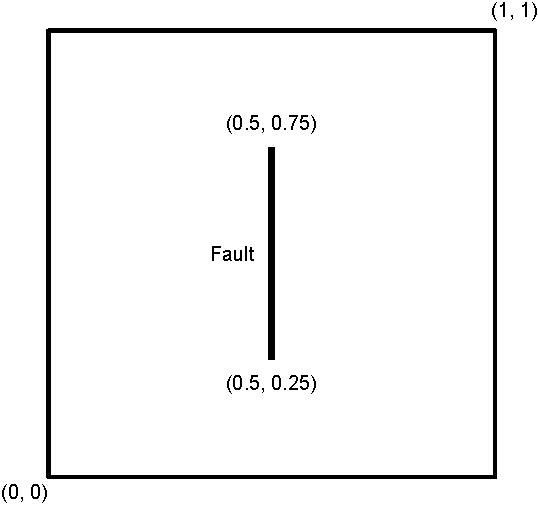
\includegraphics{Slip1}}
\caption{Domain $\Omega=[0,1]^2$ with a vertical fault of length $0.5$.}
\label{fig:slip.1}
\end{figure}
%
In this example we illustrate how to calculate the stress distribution around
a fault\index{fault} in the Earth's crust caused by a slip\index{slip} through
an earthquake.

To simplify the presentation we assume a simple domain $\Omega=[0,1]^2$ with
a vertical fault in its center as illustrated in \fig{fig:slip.1}.
We assume that the slip distribution $s_{i}$ on the fault is known.
We want to calculate the distribution of the displacements $u_{i}$\index{displacement}
and stress $\sigma_{ij}$\index{stress} in the domain.
Further, we assume an isotropic, linear elastic material model of the form
\begin{eqnarray} \label{Slip  stress}
\sigma_{ij} & = & \lambda u_{k,k} \delta_{ij} + \mu ( u_{i,j} + u_{j,i})
\end{eqnarray}
where $\lambda$ and $\mu$ are the Lam\'e coefficients\index{Lam\'e coefficients}
and $\delta_{ij}$ denotes the Kronecker symbol\index{Kronecker symbol}.
On the boundary the normal stress is given by
\begin{eqnarray} \label{Slip natural fault}
\sigma_{ij}n_{j}=0
\end{eqnarray}
and normal displacements are set to zero:
\begin{eqnarray} \label{Slip constraint}
u_{i}n_{i} =0
\end{eqnarray}
The stress needs to fulfill the momentum equation\index{momentum equation}
\begin{eqnarray}\label{Slip general problem}
- \sigma_{ij,j}=0
\end{eqnarray}
This problem is very similar to the elastic deformation problem presented in \Sec{ELASTIC CHAP}.
However, we need to address an additional challenge: the displacement
$u_{i}$ is in fact discontinuous across the fault, but we are in the
lucky situation that we know the jump of the displacements across the fault.
This is in fact the given slip $s_{i}$.
So we can split the total distribution $u_{i}$ into a component
$v_{i}$ which is continuous across the fault and the known slip $s_{i}$
\begin{eqnarray}\label{Slip Split}
u_{i} = v_{i} + \frac{1}{2} s^{\pm}_{i}
\end{eqnarray}
where $s^{\pm}=s$ when right of the fault and $s^{\pm}=-s$ when left of the fault.
We assume that $s^{\pm}=0$ when sufficiently away from the fault.

We insert this into the stress definition in \eqn{Slip stress}
\begin{eqnarray} \label{Slip stress split}
\sigma_{ij} & = &
\sigma^c_{ij} +
\frac{1}{2} \sigma^s_{ij}
\end{eqnarray}
 with
\begin{eqnarray} \label{Slip stress split 1}
\sigma^c_{ij} = \lambda v_{k,k} \delta_{ij} + \mu ( v_{i,j} + v_{j,i})
\end{eqnarray}
and
\begin{eqnarray} \label{Slip stress split 2}
\sigma^s_{ij} = \lambda s^{\pm}_{k,k} \delta_{ij} + \mu ( s^{\pm}_{i,j} + s^{\pm}_{j,i}).
\end{eqnarray}
In fact, $\sigma^s_{ij}$ defines a stress jump across the fault.
An easy way to construct this function is to use a function $\chi$ which is
$1$ on the right and $-1$ on the left side from the fault.
One can then set
\begin{eqnarray} \label{Slip  stress split 23 }
\sigma^s_{ij} = \chi \cdot  ( \lambda s_{k,k} \delta_{ij} + \mu ( s_{i,j} + s_{j,i}) )
\end{eqnarray}
assuming that $s$ is extended by zero away from the fault.
After inserting \eqn{Slip stress split} into (\ref{Slip general problem}) we
get the differential equation\index{momentum equation}
\begin{eqnarray}\label{Slip general problem 2 }
- \sigma^c_{ij,j}=\frac{1}{2} \sigma^s_{ij,j}
\end{eqnarray}
Together with the definition (\ref{Slip stress split 1}) we have a
differential equation for the continuous function $v_i$.
Notice that the boundary condition (\ref{Slip constraint}) and (\ref{Slip natural fault})
transfer to $v_i$ and $\sigma^c_{ij}$ as $s$ is zero away from the fault.
In \Sec{ELASTIC CHAP} we have discussed how this problem is solved using
the \LinearPDE class. We refer to this section for further details.

To define the fault we use the \class{FaultSystem} class introduced in \Sec{Fault System}.
The following statements define a fault system \var{fs} and add the fault \var{1} to the system:
\begin{python}
  fs=FaultSystem(dim=2)
  fs.addFault(fs.addFault(V0=[0.5,0.25], strikes=90*DEG, ls=0.5, tag=1)
\end{python}
The fault added starts at point $(0.5,0.25)$ has length $0.5$ and points north.
The main purpose of the \class{FaultSystem} class is to define a
parameterization of the fault using a local coordinate system.
One can inquire the class to get the range used to parameterize a fault.
\begin{python}
  p0,p1 = fs.getW0Range(tag=1)
\end{python}
Typically \var{p0} is equal to zero while \var{p1} is equal to the length of the fault.
The parameterization is given as a mapping from a set of local coordinates
onto a parameter range (in our case the range \var{p0} to \var{p1}).
For instance, to map the entire domain \var{mydomain} onto the fault one can
use
\begin{python}
  x = mydomain.getX()
  p,m = fs.getParametrization(x, tag=1)
\end{python}
Of course there is the problem that not all locations are on the fault.
For those locations which are on the fault \var{m} is set to 1, otherwise 0 is used.
So on return the values of \var{p} define the value of the fault parameterization
(typically the distance from the starting point of the fault along the fault)
where \var{m} is positive.
On all other locations the value of \var{p} is undefined.
Now \var{p} can be used to define a slip distribution on the fault via
\begin{python}
  s = m*(p-p0)*(p1-p)/((p1-p0)/2)**2*slip_max*[0.,1.]
\end{python}
Notice the factor \var{m} which ensures that \var{s} is zero away from the fault.
It is important that the slip is zero at the ends of the faults.

We can now put all components together to get the script:
\begin{python}
  from esys.escript import *
  from esys.escript.linearPDEs import LinearPDE
  from esys.escript.models import FaultSystem
  from esys.finley import Rectangle
  from esys.weipa import saveVTK
  from esys.escript.unitsSI import DEG

  #... set some parameters ...
  lam=1.
  mu=1
  slip_max=1.
  mydomain = Rectangle(l0=1.,l1=1.,n0=16, n1=16)  # n1 needs to be a multiple of 4!
  # .. create the fault system
  fs=FaultSystem(dim=2)
  fs.addFault(V0=[0.5,0.25], strikes=90*DEG, ls=0.5, tag=1)
  # ... create a slip distribution on the fault
  p, m=fs.getParametrization(mydomain.getX(), tag=1)
  p0,p1= fs.getW0Range(tag=1)
  s=m*(p-p0)*(p1-p)/((p1-p0)/2)**2*slip_max*[0.,1.]
  # ... calculate stress according to slip:
  D=symmetric(grad(s))
  chi, d=fs.getSideAndDistance(D.getFunctionSpace().getX(), tag=1)
  sigma_s=(mu*D+lam*trace(D)*kronecker(mydomain))*chi
  #... open symmetric PDE ...
  mypde=LinearPDE(mydomain)
  mypde.setSymmetryOn()
  #... set coefficients ...
  C=Tensor4(0., Function(mydomain))
  for i in range(mydomain.getDim()):
    for j in range(mydomain.getDim()):
       C[i,i,j,j]+=lam
       C[j,i,j,i]+=mu
       C[j,i,i,j]+=mu
  # ... fix displacement in normal direction
  x=mydomain.getX()
  msk=whereZero(x[0])*[1.,0.] + whereZero(x[0]-1.)*[1.,0.] \
     +whereZero(x[1])*[0.,1.] + whereZero(x[1]-1.)*[0.,1.]
  mypde.setValue(A=C, X=-0.5*sigma_s, q=msk)
  #... solve pde ...
  mypde.getSolverOptions().setVerbosityOn()
  v=mypde.getSolution()
  # .. write the displacement to file:
  D=symmetric(grad(v))
  sigma=(mu*D+lam*trace(D)*kronecker(mydomain))+0.5*sigma_s
  saveVTK("slip.vtu", disp=v+0.5*chi*s, stress=sigma)
\end{python}
The script creates the file \file{slip.vtu} which contains the total
displacements and stress.
These values are stored as cell-centered data.
%
\begin{figure} [ht]
\centerline{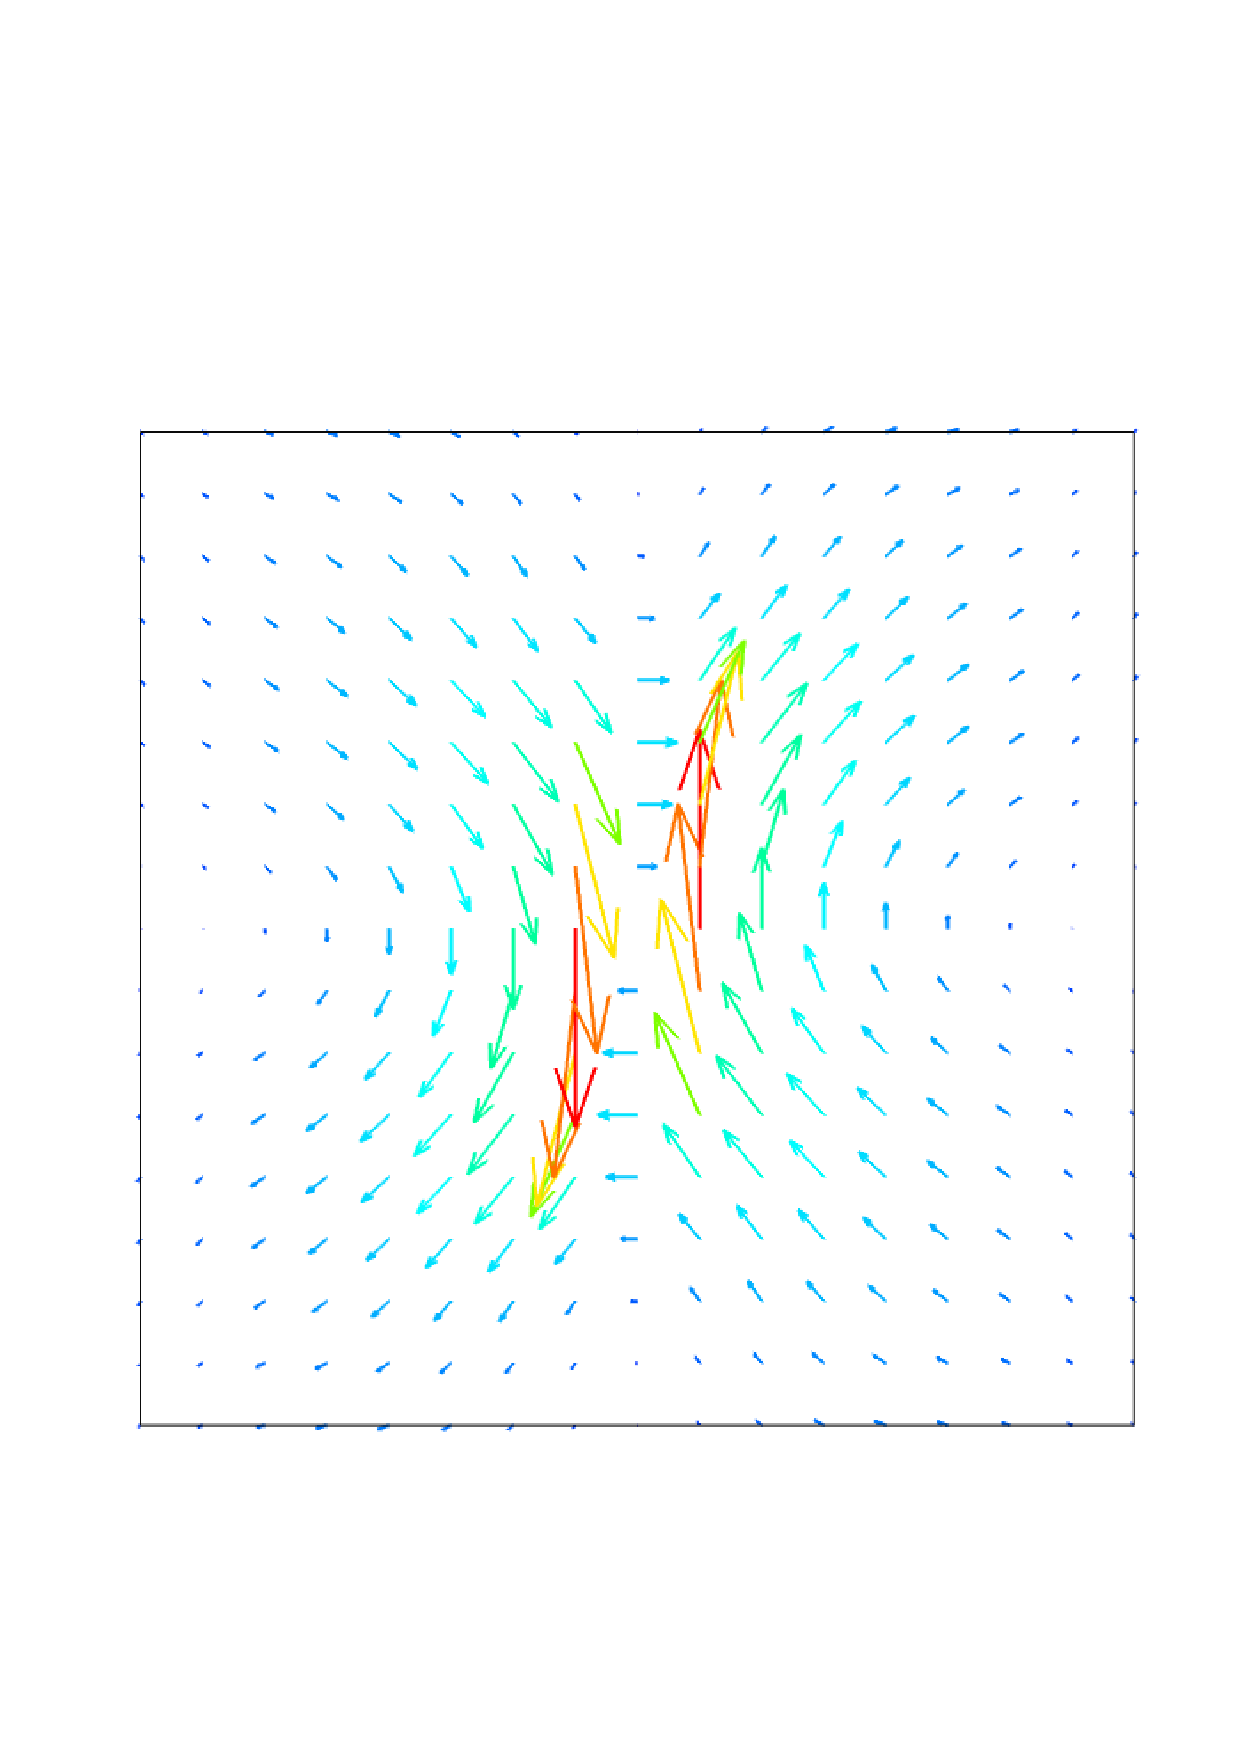
\includegraphics[width=\figwidth]{Slip2}}
\caption{Total Displacement after the slip event}
\label{fig:slip.2}
\end{figure}
%
See \fig{fig:slip.2} for a visualization of the result.






%%%%%%%%%%%%%%%%%%%%%%%%%%%%%%%%%%%%%%%%%%%%%%%%%%%%%%%%
%
% Copyright (c) 2003-2008 by University of Queensland
% Earth Systems Science Computational Center (ESSCC)
% http://www.uq.edu.au/esscc
%
% Primary Business: Queensland, Australia
% Licensed under the Open Software License version 3.0
% http://www.opensource.org/licenses/osl-3.0.php
%
%%%%%%%%%%%%%%%%%%%%%%%%%%%%%%%%%%%%%%%%%%%%%%%%%%%%%%%%


\chapter{The Module \escript}
\label{ESCRIPT CHAP}


\begin{figure}
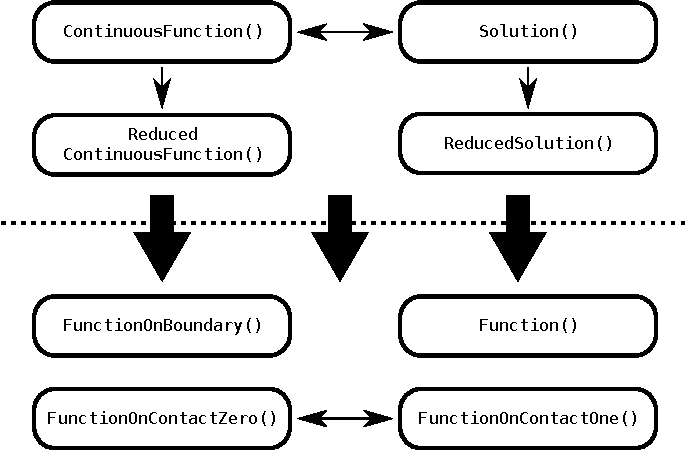
\includegraphics[width=\textwidth]{figures/EscriptDiagram1}
\caption{\label{ESCRIPT DEP}Dependency of Function Spaces in Finley. An arrow indicates that a function in the 
function space at the starting point can be interpolated to the function space of the arrow target.
All functionspaces on the left side can be interpolated to any of the functionspaces on the right.}
\end{figure}

\escript is a Python module that allows you to represent the values of
a function at points in a \Domain in such a way that the function will
be useful for the Finite Element Method (FEM) simulation.  It also
provides what we call a function space that describes how the data is
used in the simulation.  Stored along with the data is information
about the elements and nodes which will be used by \finley.

In order to understand what we mean by the term 'function space',
consider that the solution of a partial differential equation
\index{partial differential equation} (PDE) is a function on a domain
$\Omega$.  When solving a PDE using FEM, the solution is
piecewise-differentiable but, in general, its gradient is
discontinuous.  To reflect these different degrees of smoothness,
different function spaces are used.  For instance, in FEM, the
displacement field is represented by its values at the nodes of the
mesh, and so is continuous.  The strain, which is the symmetric
part of the gradient of the displacement field, is stored on the
element centers, and so is considered to be discontinuous.

A function space is described by a \FunctionSpace object.  The
following statement generates the object \var{solution_space} which is
a \FunctionSpace object and provides access to the function space of
PDE solutions on the \Domain \var{mydomain}:

\begin{python}
  solution_space=Solution(mydomain)
\end{python}
The following generators for function spaces on a \Domain \var{mydomain} are available: 
\begin{itemize}
\item \var{Solution(mydomain)}: solutions of a PDE.
\item \var{ReducedSolution(mydomain)}: solutions of a PDE with a reduced smoothness requirement.  
\item \var{ContinuousFunction(mydomain)}: continuous functions, eg. a temperature distribution.
\item \var{Function(mydomain)}: general functions which are not necessarily continuous, eg. a stress field.
\item \var{FunctionOnBoundary(mydomain)}: functions on the boundary of the domain, eg. a surface pressure.
\item \var{FunctionOnContact0(mydomain)}: functions on side $0$ of the discontinuity. 
\item \var{FunctionOnContact1(mydomain)}: functions on side $1$ of the discontinuity.
\end{itemize}

The reduced smoothness for PDE solution is often used to fulfill the Ladyzhenskaya–-Babuska–-Brezzi condition \cite{LBB} when 
solving saddle point problems \index{saddle point problems}, eg. the Stokes equation.
A discontinuity \index{discontinuity} is a region within the domain across which functions may be discontinuous.  
The location of discontinuity is defined in the \Domain object.
\fig{ESCRIPT DEP} shows the dependency between the types of function spaces in Finley (other libraries may have different relationships).

The solution of a PDE is a continuous function. Any continuous function can be seen as a general function
on the domain and can be restricted to the boundary as well as to one side of
discontinuity (the result will be different depending on 
which side is chosen). Functions on any side of the  
discontinuity can be seen as a function on the corresponding other side. 

A function on the boundary or on one side of
the discontinuity cannot be seen as a general function on the domain as there are no values 
defined for the interior. For most PDE solver libraries
the space of the solution and continuous functions is identical, however in some cases, eg.
when periodic boundary conditions are used in \finley, a solution 
fulfills periodic boundary conditions while a continuous function does not have to be periodic.

The concept of function spaces describes the properties of 
functions and allows abstraction from the actual representation 
of the function in the context of a particular application. For instance, 
in the FEM context a
function of the \Function type (written as \emph{Function()} in Figure~\ref{ESCRIPT DEP})
is usually represented by its values at the element center, 
but in a finite difference scheme the edge midpoint of cells is preferred. 
By changing its function space you can use the same function in a Finite Difference
scheme instead of Finite Element scheme.
Changing the function space of a particular function
will typically lead to a change of its representation. 
So, when seen as a general function,
a continuous function which is typically represented by its values
on the node of the FEM mesh or finite difference grid 
must be interpolated to the element centers or the cell edges,
respectively. Interpolation happens automatically in \escript
whenever it is required.

In \escript the class that stores these functions is called \Data.
The function is represented through its values on \DataSamplePoints where
the \DataSamplePoints are chosen according to the function space 
of the function.  
\Data class objects are used to define the coefficients
of the PDEs to be solved by a PDE solver library 
and also to store the solutions of the PDE.

The values of the function have a rank which gives the
number of indices, and a \Shape defining the range of each index.
The rank in \escript is limited to the range $0$ through $4$ and
it is assumed that the rank and \Shape is the same for all \DataSamplePoints.
The \Shape of a \Data object is a tuple (list) \var{s} of integers. The length
of \var{s} is the rank of the \Data object and the \var{i}-th index ranges between $0$ and $\var{s[i]}-1$.
For instance, a stress field has rank $2$ and 
\Shape $(d,d)$ where $d$ is the spatial dimension.
The following statement creates the \Data object
\var{mydat} representing a 
continuous function with values 
of \Shape $(2,3)$ and rank $2$:
\begin{python}
  mydat=Data(value=1,what=ContinuousFunction(myDomain),shape=(2,3))
\end{python}
The initial value is the constant $1$ for all \DataSamplePoints and
all components.

\Data objects can also be created from any \numarray
array or any object, such as a list of floating point numbers, 
that can be converted into a \numarrayNA \cite{NUMARRAY}. 
The following two statements
create objects which are equivalent to \var{mydat}:
\begin{python}
  mydat1=Data(value=numarray.ones((2,3)),what=ContinuousFunction(myDomain))
  mydat2=Data(value=[[1,1],[1,1],[1,1]],what=ContinuousFunction(myDomain))
\end{python}
In the first case the initial value is \var{numarray.ones((2,3))}
which generates a $2 \times 3$ matrix as a \numarrayNA 
filled with ones. The \Shape of the created \Data object
it taken from the \Shape of the array. In the second
case, the creator converts the initial value, which is a list of lists,
and converts it into a \numarrayNA before creating the actual
\Data object.      

For convenience \escript provides creators for the most common types
of \Data objects in the following forms (\var{d} defines the 
spatial dimension):
\begin{itemize}
\item \var{Scalar(0,Function(mydomain))} is the same as \var{Data(0,Function(myDomain),(,))} (each value is a scalar), 
e.g a temperature field. 
\item \var{Vector(0,Function(mydomain))} is the same as \var{Data(0,Function(myDomain),(d))} (each value is a vector), e.g
a velocity field.   
\item \var{Tensor(0,Function(mydomain))} is the same as \var{Data(0,Function(myDomain),(d,d))},
eg. a stress field.  
\item \var{Tensor4(0,Function(mydomain))} is the same as \var{Data(0,Function(myDomain),(d,d,d,d))}
eg. a Hook tensor field.   
\end{itemize}
Here the initial value is $0$ but any object that can be converted into a \numarrayNA and whose \Shape
is consistent with \Shape of the \Data object to be created can be used as the initial value.

\Data objects can be manipulated by applying unary operations (eg. cos, sin, log) point
and can be combined point-wise by applying arithmetic operations (eg. +, - ,* , /). 
It is to be emphasized that \escript itself does not handle any spatial dependencies as 
it does not know how values are interpreted by the processing PDE solver library. 
However \escript invokes interpolation if this is needed during data manipulations. 
Typically, this occurs in binary operation when both arguments belong to different
function spaces or when data are handed over to a PDE solver library 
which requires functions to be represented in a particular way. 

The following example shows the usage of {\tt Data} objects: Assume we have a
displacement field $u$ and we want to calculate the corresponding stress field
$\sigma$ using the linear--elastic isotropic material model
\begin{eqnarray}\label{eq: linear elastic stress}
\sigma\hackscore {ij}=\lambda u\hackscore {k,k} \delta\hackscore {ij} + \mu ( u\hackscore {i,j} + u\hackscore {j,i})
\end{eqnarray}
where $\delta\hackscore {ij}$ is the Kronecker symbol and 
$\lambda$ and $\mu$ are the Lame coefficients. The following function
takes the displacement {\tt u} and the Lame coefficients
\var{lam} and \var{mu} as arguments and returns the corresponding stress:
\begin{python}
  from esys.escript import *
  def getStress(u,lam,mu):
    d=u.getDomain().getDim()
    g=grad(u)
    stress=lam*trace(g)*kronecker(d)+mu*(g+transpose(g))
    return stress     
\end{python}
The variable 
\var{d} gives the spatial dimension of the 
domain on which the displacements are defined.
\var{kronecker} returns the Kronecker symbol with indexes 
$i$ and $j$ running from $0$ to \var{d}-1. The call \var{grad(u)} requires 
the displacement field \var{u} to be in the \var{Solution} or \ContinuousFunction
function space. The result \var{g} as well as the returned stress will be in the \Function function space. 
If, for example, \var{u} is the solution of a PDE then \var{getStress} might be called
in the following way:
\begin{python}
  s=getStress(u,1.,2.)
\end{python}
However \var{getStress} can also be called with \Data objects as values for
\var{lam} and \var{mu} which,
for instance in the case of a temperature dependency, are calculated by an expression. 
The following call is equivalent to the previous example:
\begin{python}
  lam=Scalar(1.,ContinuousFunction(mydomain))
  mu=Scalar(2.,Function(mydomain))
  s=getStress(u,lam,mu)
\end{python}

The function \var{lam} belongs to the \ContinuousFunction function space
but with \var{g} the function \var{trace(g)} is in the \Function function space.
In the evaluation of the product \var{lam*trace(g)} we have different function
spaces (on the nodes versus in the centers) and at first glance we have incompatible data.
\escript converts the arguments in an appropriate function space according to
Table~\ref{ESCRIPT DEP}. In this example that means
\escript sees \var{lam} as a function of the \Function function space. 
In the context of FEM this means the nodal values of 
\var{lam} are interpolated to the element centers.
The interpolation is automatic and requires no special handling.

\begin{figure}
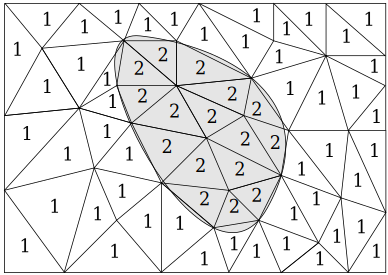
\includegraphics[width=\textwidth]{figures/EscriptDiagram2}
\caption{\label{Figure: tag}Element Tagging. A rectangular mesh over a region with two rock types {\it white} and {\it gray}.
The number in each cell refers to the major rock type present in the cell ($1$ for {\it white} and $2$ for {\it gray}).
}
\end{figure}

Material parameters such as the Lame coefficients are typically dependent on rock types present in the 
area of interest. A common technique to handle these kinds of material parameters is "tagging", which
uses storage efficiently. \fig{Figure: tag}
shows an example. In this case two rock types {\it white} and {\it gray} can be found in the domain. The domain
is subdivided into triangular shaped cells. Each 
cell has a tag indicating the rock type predominately found in this cell. Here $1$ is used to indicate
rock type {\it white} and $2$ for rock type {\it gray}. The tags are assigned at the time when the cells are generated
and stored in the \Domain class object. To allow easier usage of tags, names can be used instead of numbers. These names are typically defined 
at the time when the geometry is generated. 

The following statements show how, for the
example of \fig{Figure: tag}, the stress calculation discussed above and tagged values are used for
\var{lam}:
\begin{python}
  lam=Scalar(value=2.,what=Function(mydomain))
  insertTaggedValue(lam,white=30.,gray=5000.)
  s=getStress(u,lam,2.)
\end{python}
In this example \var{lam} is set to $30$ for those cells with tag {\it white} (=$1$) and to $5000.$ for those cells 
with tag {\it gray} (=$2$_. The initial value $2$ of \var{lam} is used as a default value for the case when a tag
is encountered which has not been linked with a value. The \var{getStress} method
does not need to be changed now that we are using tags.
\escript resolves the tags when \var{lam*trace(g)} is calculated.

This brings us to a very important point about \escript.
You can develop a simulation with constant Lame coefficients, and then later switch to tagged
Lame coefficients without otherwise changing your python script.
In short, you can use the same script to model with different domains and different types of input data.

There are three main ways in which \Data objects are represented internally: constant, tagged, and expanded.
In the constant case, the same value is used at each sample point and only a single value is stored to save memory. 
In the expanded case, each sample point has an individual value (such as for the solution of a PDE).
This is where your largest data sets will be created because the values are stored as a complete array.
The tagged case has already been discussed above.

Expanded data is created when you create a \Data object with expanded=True.
Tagged data sets are created when you use the insertTaggedValue() method as shown above.
 
Values are accessed through a sample reference number. Operations on expanded \Data
objects have to be performed for each sample point individually. When tagged values are used, the values are
held in a dictionary. Operations on tagged data require processing the set of tagged values only, rather than 
processing the value for each individual sample point. 
\escript allows any mixture of constant, tagged and expanded data in a single expression.

\Data objects can be written to disk files and read with \var{dump} and \var{load}, both of which use \netCDF\cite{NETCDF}.
Use these to save data for visualization, checkpoint/restart or simply to save and reuse data that was expensive to compute.

For instance to save the coordinates of the data points of the
\ContinuousFunction to the file {\tt x.nc} use 
\begin{python}
  x=ContinuousFunction(mydomain).getX()
  x.dump("x.nc")
  mydomain.dump(`dom.nc`)
\end{python}
To recover the object \var{x} and \var{mydomain} was a \finley mesh use
\begin{python}
  from esys.finley import LoadMesh
  mydomain=LoadMesh('dom.nc')
  x=load("x.nc", mydomain)
\end{python}
It possible to rerun the mechanism that was originally used to generates
\var{mydomain} to recreate \var{mydomain}. However in most cases using \var{dump} and
load is faster in particuar if optimization has been applied. In case that
\escript is running on more than one \MPI processor the \var{dump} will create an individual file for each processor containing the local data. In order to avoid conflicts the file name is extended by the \MPI processor rank.

The function space of the \Data is stored in {\tt x.nc}, though.
If the \Data object
is expanded, the number of data points in the file and of the \Domain for the particular \FunctionSpace must match. 
Moreover, the ordering of the values is checked using the reference identifiers provided by 
\FunctionSpace on the \Domain. In some cases, data points will be re-ordered. Take care to be sure you get what you want!


\section{\escript Classes}
\declaremodule{extension}{esys.escript} 
\modulesynopsis{Data manipulation}

\subsection{\Domain class}
\begin{classdesc}{Domain}{}
A \Domain object is used to describe a geometric region together with 
a way of representing functions over this region.
The \Domain class provides an abstract interface to the domain of \FunctionSpace and \Data objects.
\Domain needs to be subclassed in order to provide a complete implementation.
\end{classdesc}
The following methods are available:
\begin{methoddesc}[Domain]{getDim}{}
returns the spatial dimension of the \Domain.
\end{methoddesc}
\begin{methoddesc}[Domain]{dump}{filename}
dumps the \Domain into the file \var{filename}.
\end{methoddesc}
\begin{methoddesc}[Domain]{getX}{}
returns the locations in the \Domain. The \FunctionSpace of the returned
\Data object is chosen by the \Domain implementation. Typically it will be
in the \Function.
\end{methoddesc}

\begin{methoddesc}[Domain]{setX}{newX}
assigns a new location to the \Domain. \var{newX} has to have \Shape $(d,)$
where $d$ is the spatial dimension of the domain. Typically \var{newX} must be
in the \ContinuousFunction but the space actually to be used depends on the \Domain implementation.
\end{methoddesc}

\begin{methoddesc}[Domain]{getNormal}{}
returns the surface normals on the boundary of the \Domain as \Data object.
\end{methoddesc}

\begin{methoddesc}[Domain]{getSize}{}
returns the local sample size, e.g. the element diameter, as \Data object.
\end{methoddesc}

\begin{methoddesc}[Domain]{setTagMap}{tag_name, tag}
defines a mapping of the tag name  \var{tag_name} to the \var{tag}. 
\end{methoddesc}
\begin{methoddesc}[Domain]{getTag}{tag_name}
returns the tag associated with the tag name \var{tag_name}.
\end{methoddesc}
\begin{methoddesc}[Domain]{isValidTagName}{tag_name}
return \True if \var{tag_name} is a valid tag name.
\end{methoddesc}

\begin{methoddesc}[Domain]{__eq__}{arg}
(python == operator) returns \True if the \Domain \var{arg} describes the same domain. Otherwise
\False is returned.
\end{methoddesc}

\begin{methoddesc}[Domain]{__ne__}{arg}
(python != operator) returns \True if the \Domain \var{arg} does not describe the same domain. 
Otherwise \False is returned.
\end{methoddesc}

\begin{methoddesc}[Domain]{__str__}{arg}
(python str() function) returns string representation of the \Domain.
\end{methoddesc}

\begin{methoddesc}[Domain]{onMasterProcessor)}{}
returns \True if the processor is the master processor within 
the \MPI processor group used by the \Domain. This is the processor with rank 0.
If \MPI support is not enabled the return value is always \True.
\end{methoddesc}

\begin{methoddesc}[Domain]{getMPISize}{}
 returns the number of \MPI processors used for this \Domain. If \MPI support is not enabled
1 is returned.
\end{methoddesc}

\begin{methoddesc}[Domain]{getMPIRank}{}
 returns the rank of the processor executing the statement 
within the  \MPI processor group used by the \Domain. 
If \MPI support is not enabled 0 is returned.
\end{methoddesc}

\begin{methoddesc}[Domain]{MPIBarrier}{}
executes barrier synchronization within 
the \MPI processor group used by the \Domain.
If \MPI support is not enabled, this command does nothing. 
\end{methoddesc}

\subsection{\FunctionSpace class}
\begin{classdesc}{FunctionSpace}{}
\FunctionSpace objects are used to define properties of \Data objects, such as continuity. \FunctionSpace objects
are instantiated by generator functions. A \Data object in a particular \FunctionSpace is 
represented by its values at \DataSamplePoints which are defined by the type and the \Domain of the
\FunctionSpace.
\end{classdesc}
The following methods are available:
\begin{methoddesc}[FunctionSpace]{getDim}{}
returns the spatial dimension of the \Domain of the \FunctionSpace.
\end{methoddesc}



\begin{methoddesc}[FunctionSpace]{getX}{}
returns the location of the \DataSamplePoints.
\end{methoddesc}

\begin{methoddesc}[FunctionSpace]{getNormal}{}
If the domain of functions in the \FunctionSpace 
is a hyper-manifold (e.g. the boundary of a domain)
the method returns the outer normal at each of the 
\DataSamplePoints. Otherwise an exception is raised.
\end{methoddesc}

\begin{methoddesc}[FunctionSpace]{getSize}{}
returns a \Data objects measuring the spacing of the \DataSamplePoints.  
The size may be zero.
\end{methoddesc}

\begin{methoddesc}[FunctionSpace]{getDomain}{}
returns the \Domain of the \FunctionSpace.
\end{methoddesc}

\begin{methoddesc}[FunctionSpace]{setTags}{new_tag, mask}
assigns a new tag \var{new_tag} to all data sample 
where \var{mask} is positive for a least one data point. 
\var{mask} must be defined on the this \FunctionSpace.
Use the \var{setTagMap} to assign a tag name to \var{new_tag}.
\end{methoddesc}

\begin{methoddesc}[FunctionSpace]{__eq__}{arg}
(python == operator) returns \True if the \Domain \var{arg} describes the same domain. Otherwise
\False is returned.
\end{methoddesc}

\begin{methoddesc}[FunctionSpace]{__ne__}{arg}
(python != operator) returns \True if the \Domain \var{arg} do not describe the same domain. 
Otherwise \False is returned.
\end{methoddesc}

\begin{methoddesc}[Domain]{__str__}{g}
(python str() function) returns string representation of the \Domain.
\end{methoddesc}

The following function provide generators for \FunctionSpace objects:
\begin{funcdesc}{Function}{domain}
returns the \Function on the \Domain \var{domain}. \Data objects in this type of \Function
are defined over the whole geometric region defined by \var{domain}. 
\end{funcdesc}

\begin{funcdesc}{ContinuousFunction}{domain}
returns the \ContinuousFunction on the \Domain domain. \Data objects in this type of \Function
are defined over the whole geometric region defined by \var{domain} and assumed to represent
a continuous function.
\end{funcdesc}

\begin{funcdesc}{FunctionOnBoundary}{domain}
returns the \ContinuousFunction on the \Domain domain. \Data objects in this type of \Function
are defined on the boundary of the geometric region defined by \var{domain}. 
\end{funcdesc}

\begin{funcdesc}{FunctionOnContactZero}{domain}
returns the \FunctionOnContactZero the \Domain domain. \Data objects in this type of \Function
are defined on side 0 of a discontinuity  within the geometric region defined by \var{domain}.
The discontinuity is defined when \var{domain} is instantiated.
\end{funcdesc}

\begin{funcdesc}{FunctionOnContactOne}{domain}
returns the \FunctionOnContactOne on the \Domain domain. 
\Data objects in this type of \Function
are defined on side 1 of a discontinuity  within the geometric region defined by \var{domain}.
The discontinuity is defined when \var{domain} is instantiated.
\end{funcdesc}

\begin{funcdesc}{Solution}{domain}
returns the \SolutionFS on the \Domain domain. \Data objects in this type of \Function
are defined on geometric region defined by \var{domain} and are solutions of
partial differential equations \index{partial differential equation}. 
\end{funcdesc}

\begin{funcdesc}{ReducedSolution}{domain}
returns the \ReducedSolutionFS on the \Domain domain. \Data objects in this type of \Function
are defined on geometric region defined by \var{domain} and are solutions of
partial differential equations \index{partial differential equation} with a reduced smoothness 
for the solution approximation.
\end{funcdesc}

\subsection{\Data Class}
\label{SEC ESCRIPT DATA}

The following table shows arithmetic operations that can be performed point-wise on
\Data objects.
\begin{tableii}{l|l}{textrm}{expression}{Description}
\lineii{+\var{arg0}} {identical to \var{arg} \index{+}}
\lineii{-\var{arg0}} {negation\index{-}}
\lineii{\var{arg0}+\var{arg1}} {adds \var{arg0} and \var{arg1} \index{+}}
\lineii{\var{arg0}*\var{arg1}} {multiplies \var{arg0} and \var{arg1} \index{*}}
\lineii{\var{arg0}-\var{arg1}} {difference \var{arg1} from\var{arg1} \index{-}}
\lineii{\var{arg0}/\var{arg1}} {divide \var{arg0} by \var{arg1} \index{/}}
\lineii{\var{arg0}**\var{arg1}} {raises \var{arg0} to the power of \var{arg1} \index{**}}
\end{tableii}
At least one of the arguments \var{arg0} or \var{arg1} must be a
\Data object.
Either of the arguments may be a \Data object, a python number or a numarray object.

If \var{arg0} or \var{arg1} are
not defined on the same \FunctionSpace, then an attempt is made to convert \var{arg0}
to the \FunctionSpace of \var{arg1} or to convert \var{arg1} to
the \FunctionSpace of \var{arg0}. Both arguments must have the same
\Shape or one of the arguments may be of rank 0 (a constant).

The returned \Data object has the same \Shape and is defined on
the \DataSamplePoints as \var{arg0} or \var{arg1}.

The following table shows the update operations that can be applied to
\Data objects:
\begin{tableii}{l|l}{textrm}{expression}{Description}
\lineii{\var{arg0}+=\var{arg2}} {adds \var{arg0} to \var{arg2} \index{+}}
\lineii{\var{arg0}*=\var{arg2}} {multiplies \var{arg0} with \var{arg2} \index{*}}
\lineii{\var{arg0}-=\var{arg2}} {subtracts \var{arg2} from\var{arg2} \index{-}}
\lineii{\var{arg0}/=\var{arg2}} {divides \var{arg0} by \var{arg2} \index{/}}
\lineii{\var{arg0}**=\var{arg2}} {raises \var{arg0} by \var{arg2} \index{**}}
\end{tableii}
\var{arg0} must be a \Data object. \var{arg1} must be a
\Data object or an object that can be converted into a
\Data object. \var{arg1} must have the same \Shape as
\var{arg0} or have rank 0.  In the latter case it is
assumed that the values of \var{arg1} are constant for all
components. \var{arg1} must be defined in the same \FunctionSpace as
\var{arg0} or it must be possible to interpolate \var{arg1} onto the
\FunctionSpace of \var{arg0}.

The \Data class supports taking slices from a \Data object as well as assigning new values to a slice of an existing
\Data object. \index{slicing}
The following expressions for taking and setting slices are valid:
\begin{tableiii}{l|ll}{textrm}{rank of \var{arg}}{slicing expression}{\Shape of returned and assigned object}
\lineiii{0}{ no slicing }                      {-}
\lineiii{1}{\var{arg[l0:u0]}}                   {(\var{u0}-\var{l0},)}
\lineiii{2}{\var{arg[l0:u0,l1:u1]}}             {(\var{u0}-\var{l0},\var{u1}-\var{l1})}
\lineiii{3}{\var{arg[l0:u0,l1:u1,l2:u2]} }      {(\var{u0}-\var{l0},\var{u1}-\var{l1},\var{u2}-\var{l2})}
\lineiii{4}{\var{arg[l0:u0,l1:u1,l2:u2,l3:u3]}} {(\var{u0}-\var{l0},\var{u1}-\var{l1},\var{u2}-\var{l2},\var{u3}-\var{l3})}
\end{tableiii}
where \var{s} is the \Shape of \var{arg} and 
\[0 \le \var{l0} \le \var{u0} \le \var{s[0]},\]
\[0 \le \var{l1} \le \var{u1} \le \var{s[1]},\] 
\[0 \le \var{l2} \le \var{u2} \le \var{s[2]},\] 
\[0 \le \var{l3} \le \var{u3} \le \var{s[3]}.\]
Any of the lower indexes \var{l0}, \var{l1}, \var{l2} and \var{l3} may not be present in which case 
$0$ is assumed. 
Any of the upper indexes \var{u0}, \var{u1}, \var{u2} and \var{u3} may be omitted, in which case, the upper limit for that dimension is assumed. 
The lower and upper index may be identical, in which case the column and the lower or upper
index may be dropped. In the returned or in the object assigned to a slice, the corresponding component is dropped,
i.e. the rank is reduced by one in comparison to \var{arg}.
The following examples show slicing in action:
\begin{python}
  t=Data(1.,(4,4,6,6),Function(mydomain))
  t[1,1,1,0]=9.
  s=t[:2,:,2:6,5] # s has rank 3
  s[:,:,1]=1.
  t[:2,:2,5,5]=s[2:4,1,:2]
\end{python}

\subsection{Generation of \Data objects}
\begin{classdesc}{Data}{value=0,shape=(,),what=FunctionSpace(),expand=\False}
creates a \Data object with \Shape \var{shape} in the \FunctionSpace \var{what}.
The values at all \DataSamplePoints are set to the double value \var{value}. If \var{expanded} is \True
the \Data object is represented in expanded from.
\end{classdesc}

\begin{classdesc}{Data}{value,what=FunctionSpace(),expand=\False}
creates a \Data object in the \FunctionSpace \var{what}. 
The value for each \DataSamplePoints is set to \var{value}, which could be a \numarray, \Data object \var{value} or a dictionary of 
\numarray or floating point numbers. In the latter case the keys must be integers and are used
as tags.
The \Shape of the returned object is equal to the \Shape of \var{value}. If \var{expanded} is \True
the \Data object is represented in expanded form.
\end{classdesc}

\begin{classdesc}{Data}{}
creates an \EmptyData object. The \EmptyData object is used to indicate that an argument is not present
where a \Data object is required.
\end{classdesc}

\begin{funcdesc}{Scalar}{value=0.,what=FunctionSpace(),expand=\False}
returns a \Data object of rank 0 (a constant) in the \FunctionSpace \var{what}.
Values are initialized with \var{value}, a double precision quantity. If \var{expanded} is \True
the \Data object is represented in expanded from.
\end{funcdesc}

\begin{funcdesc}{Vector}{value=0.,what=FunctionSpace(),expand=\False}
returns a \Data object of \Shape \var{(d,)} in the \FunctionSpace \var{what},
where \var{d} is the spatial dimension of the \Domain of \var{what}.
Values are initialed with \var{value}, a double precision quantity. If \var{expanded} is \True
the \Data object is represented in expanded from.
\end{funcdesc}

\begin{funcdesc}{Tensor}{value=0.,what=FunctionSpace(),expand=\False}
returns a \Data object of \Shape \var{(d,d)} in the \FunctionSpace \var{what},
where \var{d} is the spatial dimension of the \Domain of \var{what}.
Values are initialed with \var{value}, a double precision quantity. If \var{expanded} is \True
the \Data object is represented in expanded from.
\end{funcdesc}

\begin{funcdesc}{Tensor3}{value=0.,what=FunctionSpace(),expand=\False}
returns a \Data object of \Shape \var{(d,d,d)} in the \FunctionSpace \var{what},
where \var{d} is the spatial dimension of the \Domain of \var{what}.
Values are initialed with \var{value}, a double precision quantity. If \var{expanded} is \True
the \Data object is re\var{arg}presented in expanded from.
\end{funcdesc}

\begin{funcdesc}{Tensor4}{value=0.,what=FunctionSpace(),expand=\False}
returns a \Data object of \Shape \var{(d,d,d,d)} in the \FunctionSpace \var{what},
where \var{d} is the spatial dimension of the \Domain of \var{what}.
Values are initialized with \var{value}, a double precision quantity. If \var{expanded} is \True
the \Data object is represented in expanded from.
\end{funcdesc}

\begin{funcdesc}{load}{filename,domain}
recovers a \Data object on \Domain \var{domain} from the file \var{filename}, which was created by \function{dump}.
\end{funcdesc}

\subsection{\Data methods}
These are the most frequently-used methods of the 
\Data class. A complete list of methods can be found on \ReferenceGuide.
\begin{methoddesc}[Data]{getFunctionSpace}{}
returns the \FunctionSpace of the object.
\end{methoddesc}

\begin{methoddesc}[Data]{getDomain}{}
returns the \Domain  of the object.
\end{methoddesc}

\begin{methoddesc}[Data]{getShape}{}
returns the \Shape  of the object as a \class{tuple} of
integers.
\end{methoddesc}

\begin{methoddesc}[Data]{getRank}{}
returns the rank of the data on each data point. \index{rank}
\end{methoddesc}

\begin{methoddesc}[Data]{isEmpty}{}
returns \True id the \Data object is the \EmptyData object.
Otherwise \False is returned.
Note that this is not the same as asking if the object contains no \DataSamplePoints.
\end{methoddesc}

\begin{methoddesc}[Data]{setTaggedValue}{tag_name,value}
assigns the \var{value} to all \DataSamplePoints which have the tag
assigned to \var{tag_name}. \var{value} must be an object of class
\class{numarray.NumArray} or must be convertible into a
\class{numarray.NumArray} object. \var{value} (or the corresponding
\class{numarray.NumArray} object) must be of rank $0$ or must have the
same rank like the object.
If a value has already be defined for tag \var{tag_name} within the object
it is overwritten by the new \var{value}.  If the object is expanded,
the value assigned to \DataSamplePoints with tag \var{tag_name} is replaced by
\var{value}. If no tag is assigned tag name \var{tag_name}, no value is set.
\end{methoddesc}

\begin{methoddesc}[Data]{dump}{filename}
dumps the \Data object to the file \var{filename}. The file stores the
function space but not the \Domain. It is in the responsibility of the user to
save the \Domain. 
\end{methoddesc}

\begin{methoddesc}[Data]{__str__}{}
returns a string representation of the object.
\end{methoddesc}

\subsection{Functions of \Data objects}
This section lists the most important functions for \Data class objects \var{a}.
A complete list and a more detailed description of the functionality can be found on \ReferenceGuide.
\begin{funcdesc}{saveVTK}{filename,**kwdata}
writes \Data defined by keywords in the file with \var{filename} using the 
vtk file format \VTK file format. The key word is used as an identifier. The statement
\begin{python}
  saveVTK("out.xml",temperature=T,velocity=v)
\end{python} 
will write the scalar \var{T} as \var{temperature} and the vector \var{v} as  \var{velocity} into the 
file \file{out.xml}. Restrictions on the allowed combinations of \FunctionSpace apply.
\end{funcdesc}
\begin{funcdesc}{saveDX}{filename,**kwdata}
writes \Data defined by keywords in the file with \var{filename} using the 
vtk file format \OpenDX file format. The key word is used as an identifier. The statement
\begin{python}
  saveDX("out.dx",temperature=T,velocity=v)
\end{python} 
will write the scalar \var{T} as \var{temperature} and the vector \var{v} as  \var{velocity} into the 
file \file{out.dx}. Restrictions on the allowed combinations of \FunctionSpace apply.
\end{funcdesc}
\begin{funcdesc}{kronecker}{d}
returns a \RankTwo \Data object in \FunctionSpace \var{d} such that
\begin{equation}
\code{kronecker(d)}\left[ i,j\right] = \left\{ 
\begin{array}{cc}
1 & \mbox{ if } i=j \\
0 & \mbox{ otherwise }
\end{array}
\right.
\end{equation}
If \var{d} is an integer a $(d,d)$ \numarray array is returned.
\end{funcdesc}
\begin{funcdesc}{identityTensor}{d}
is a synonym for \code{kronecker} (see above).
% returns a \RankTwo \Data object in \FunctionSpace \var{d} such that
% \begin{equation}
% \code{identityTensor(d)}\left[ i,j\right] = \left\{ 
% \begin{array}{cc}
% 1 & \mbox{ if } i=j \\
% 0 & \mbox{ otherwise }
% \end{array}
% \right.
% \end{equation}
% If \var{d} is an integer a $(d,d)$ \numarray array is returned.
\end{funcdesc}
\begin{funcdesc}{identityTensor4}{d}
returns a \RankFour \Data object in \FunctionSpace \var{d} such that
\begin{equation}
\code{identityTensor(d)}\left[ i,j,k,l\right] = \left\{ 
\begin{array}{cc}
1 & \mbox{ if } i=k \mbox{ and } j=l\\
0 & \mbox{ otherwise }
\end{array}
\right.
\end{equation}
If \var{d} is an integer a $(d,d,d,d)$ \numarray array is returned.
\end{funcdesc}
\begin{funcdesc}{unitVector}{i,d}
returns a \RankOne \Data object in \FunctionSpace \var{d} such that
\begin{equation}
\code{identityTensor(d)}\left[ j \right] = \left\{ 
\begin{array}{cc}
1 & \mbox{ if } j=i\\
0 & \mbox{ otherwise }
\end{array}
\right.
\end{equation}
If \var{d} is an integer a $(d,)$ \numarray array is returned.

\end{funcdesc}

\begin{funcdesc}{Lsup}{a}
returns the $L^{sup}$ norm of \var{arg}. This is the maximum of the absolute values
 over all components and all \DataSamplePoints of \var{a}. 
\end{funcdesc}

\begin{funcdesc}{sup}{a}
returns the maximum value over all components and all \DataSamplePoints of \var{a}.
\end{funcdesc}

\begin{funcdesc}{inf}{a}
returns the minimum value over all components and all \DataSamplePoints of \var{a}
\end{funcdesc}



\begin{funcdesc}{minval}{a}
returns at each \DataSamplePoints the minimum value over all components.
\end{funcdesc}

\begin{funcdesc}{maxval}{a}
returns at each \DataSamplePoints the maximum value over all components.
\end{funcdesc}

\begin{funcdesc}{length}{a}
returns at Euclidean norm at each \DataSamplePoints. For a \RankFour \var{a} this is
\begin{equation}
\code{length(a)}=\sqrt{\sum\hackscore{ijkl} \var{a} \left[i,j,k,l\right]^2}
\end{equation} 
\end{funcdesc}
\begin{funcdesc}{trace}{a\optional{,axis_offset=0}}
returns the trace of \var{a}. This is the sum over components \var{axis_offset} and \var{axis_offset+1} with the same index. For instance in the
case of a \RankTwo function and this is 
\begin{equation}
\code{trace(a)}=\sum\hackscore{i} \var{a} \left[i,i\right]
\end{equation} 
and for a \RankFour function and  \code{axis_offset=1} this is
\begin{equation}
\code{trace(a,1)}\left[i,j\right]=\sum\hackscore{k} \var{a} \left[i,k,k,j\right]
\end{equation} 
\end{funcdesc}

\begin{funcdesc}{transpose}{a\optional{, axis_offset=None}}
returns the transpose of \var{a}. This swaps the first \var{axis_offset} components of \var{a} with the rest. If \var{axis_offset} is not
present \code{int(r/2)} is used where \var{r} is the rank of \var{a}. 
 the sum over components \var{axis_offset} and \var{axis_offset+1} with the same index. For instance in the
case of a \RankTwo function and this is 
\begin{equation}
\code{transpose(a)}\left[i,j\right]=\var{a} \left[j,i\right]
\end{equation} 
and for a \RankFour function and  \code{axis_offset=1} this is
\begin{equation}
\code{transpose(a,1)}\left[i,j,k,l\right]=\var{a} \left[j,k,l,i\right]
\end{equation} 
\end{funcdesc}

\begin{funcdesc}{swap_axes}{a\optional{, axis0=0 \optional{, axis1=1 }}}
returns \var{a} but with swapped components \var{axis0} and  \var{axis1}. The argument \var{a} must be
at least of \RankTwo. For instance in the 
for a \RankFour argument, \code{axis0=1} and \code{axis1=2} this is
\begin{equation}
\code{swap_axes(a,1,2)}\left[i,j,k,l\right]=\var{a} \left[i,k,j,l\right]
\end{equation} 
\end{funcdesc}

\begin{funcdesc}{symmetric}{a}
returns the symmetric part of \var{a}. This is \code{(a+transpose(a))/2}.
\end{funcdesc}
\begin{funcdesc}{nonsymmetric}{a}
returns the non--symmetric part of \var{a}. This is \code{(a-transpose(a))/2}.
\end{funcdesc}
\begin{funcdesc}{inverse}{a}
return the inverse of \var{a}. This is 
\begin{equation}
\code{matrix_mult(inverse(a),a)=kronecker(d)}
\end{equation} 
if \var{a} has shape \code{(d,d)}. The current implementation is restricted to arguments of shape 
\code{(2,2)} and \code{(3,3)}.
\end{funcdesc}
\begin{funcdesc}{eigenvalues}{a}
return the eigenvalues of \var{a}. This is 
\begin{equation}
\code{matrix_mult(a,V)=e[i]*V}
\end{equation} 
where \code{e=eigenvalues(a)} and \var{V} is suitable non--zero vector \var{V}. 
The eigenvalues are ordered in increasing size.
The argument \var{a} has to be the symmetric, ie. \code{a=symmetric(a)}.  
The current implementation is restricted to arguments of shape 
\code{(2,2)} and \code{(3,3)}.
\end{funcdesc}
\begin{funcdesc}{eigenvalues_and_eigenvectors}{a}
return the eigenvalues and eigenvectors of \var{a}. This is 
\begin{equation}
\code{matrix_mult(a,V[:,i])=e[i]*V[:,i]}
\end{equation} 
where \code{e,V=eigenvalues_and_eigenvectors(a)}. The eigenvectors \var{V} are orthogonal and normalized, ie.
\begin{equation}
\code{matrix_mult(transpose(V),V)=kronecker(d)}
\end{equation} 
if \var{a} has shape \code{(d,d)}. The eigenvalues are ordered in increasing size.
The argument \var{a} has to be the symmetric, ie. \code{a=symmetric(a)}.  
The current implementation is restricted to arguments of shape 
\code{(2,2)} and \code{(3,3)}.
\end{funcdesc}
\begin{funcdesc}{maximum}{*a}
returns the maximum value over all arguments at all \DataSamplePoints and for each component.
For instance 
\begin{equation}
\code{maximum(a0,a1)}\left[i,j\right]=max(\var{a0} \left[i,j\right],\var{a1} \left[i,j\right])
\end{equation}
at all \DataSamplePoints.
\end{funcdesc}
\begin{funcdesc}{minimum}{*a}
returns the minimum value over all arguments at all \DataSamplePoints and for each component.
For instance 
\begin{equation}
\code{minimum(a0,a1)}\left[i,j\right]=min(\var{a0} \left[i,j\right],\var{a1} \left[i,j\right])
\end{equation}
at all \DataSamplePoints.
\end{funcdesc}

\begin{funcdesc}{clip}{a\optional{, minval=0.}\optional{, maxval=1.}}
cuts back \var{a} into the range between \var{minval} and \var{maxval}. A value in the returned object equals 
\var{minval} if the corresponding value of \var{a} is less than \var{minval}, equals \var{maxval} if the 
 corresponding value of \var{a} is greater than \var{maxval}
or corresponding value of \var{a} otherwise.
\end{funcdesc}
\begin{funcdesc}{inner}{a0,a1}
returns the inner product of \var{a0} and \var{a1}. For instance in the
case of \RankTwo arguments and this is 
\begin{equation}
\code{inner(a)}=\sum\hackscore{ij}\var{a0} \left[j,i\right]  \cdot \var{a1} \left[j,i\right]
\end{equation} 
and for a \RankFour arguments this is
\begin{equation}
\code{inner(a)}=\sum\hackscore{ijkl}\var{a0} \left[i,j,k,l\right]  \cdot \var{a1} \left[j,i,k,l\right]
\end{equation} 
\end{funcdesc}

\begin{funcdesc}{matrix_mult}{a0,a1}
returns the matrix product of \var{a0} and \var{a1}. If \var{a1} is \RankOne this is
\begin{equation}
\code{matrix_mult(a)}\left[i\right]=\sum\hackscore{k}\var{a0}  \cdot \left[i,k\right]\var{a1} \left[k\right]
\end{equation} 
and if \var{a1} is \RankTwo this is
\begin{equation}
\code{matrix_mult(a)}\left[i,j\right]=\sum\hackscore{k}\var{a0}  \cdot \left[i,k\right]\var{a1} \left[k,j\right]
\end{equation} 
\end{funcdesc}

\begin{funcdesc}{transposed_matrix_mult}{a0,a1}
returns the matrix product of the transposed of \var{a0} and \var{a1}. The function is equivalent to 
\code{matrix_mult(transpose(a0),a1)}.
If \var{a1} is \RankOne this is
\begin{equation}
\code{transposed_matrix_mult(a)}\left[i\right]=\sum\hackscore{k}\var{a0}  \cdot \left[k,i\right]\var{a1} \left[k\right]
\end{equation} 
and if \var{a1} is \RankTwo this is
\begin{equation}
\code{transposed_matrix_mult(a)}\left[i,j\right]=\sum\hackscore{k}\var{a0}  \cdot \left[k,i\right]\var{a1} \left[k,j\right]
\end{equation} 
\end{funcdesc}

\begin{funcdesc}{matrix_transposed_mult}{a0,a1}
returns the matrix product of \var{a0} and the transposed of \var{a1}.
The function is equivalent to
\code{matrix_mult(a0,transpose(a1))}.  
If \var{a1} is \RankTwo this is
\begin{equation}
\code{matrix_transposed_mult(a)}\left[i,j\right]=\sum\hackscore{k}\var{a0}  \cdot \left[i,k\right]\var{a1} \left[j,k\right]
\end{equation} 
\end{funcdesc}

\begin{funcdesc}{outer}{a0,a1}
returns the outer product of \var{a0} and \var{a1}. For instance if \var{a0} and \var{a1} both are \RankOne then
\begin{equation}
\code{outer(a)}\left[i,j\right]=\var{a0} \left[i\right]  \cdot  \var{a1}\left[j\right]
\end{equation} 
and if \var{a0} is \RankOne and \var{a1} is \RankThree
\begin{equation}
\code{outer(a)}\left[i,j,k\right]=\var{a0} \left[i\right] \cdot \var{a1}\left[j,k\right]
\end{equation} 
\end{funcdesc}

\begin{funcdesc}{tensor_mult}{a0,a1}
returns the tensor product of \var{a0} and \var{a1}. If \var{a1} is \RankTwo this is
\begin{equation}
\code{tensor_mult(a)}\left[i,j\right]=\sum\hackscore{kl}\var{a0}\left[i,j,k,l\right] \cdot \var{a1} \left[k,l\right]
\end{equation} 
and if \var{a1} is \RankFour this is
\begin{equation}
\code{tensor_mult(a)}\left[i,j,k,l\right]=\sum\hackscore{mn}\var{a0} \left[i,j,m,n\right] \cdot \var{a1} \left[m,n,k,l\right]
\end{equation} 
\end{funcdesc}

\begin{funcdesc}{transposed_tensor_mult}{a0,a1}
returns the tensor product of the transposed of \var{a0} and \var{a1}. The function is equivalent to
\code{tensor_mult(transpose(a0),a1)}.
If \var{a1} is \RankTwo this is
\begin{equation}
\code{transposed_tensor_mult(a)}\left[i,j\right]=\sum\hackscore{kl}\var{a0}\left[k,l,i,j\right] \cdot \var{a1} \left[k,l\right]
\end{equation} 
and if \var{a1} is \RankFour this is
\begin{equation}
\code{transposed_tensor_mult(a)}\left[i,j,k,l\right]=\sum\hackscore{mn}\var{a0} \left[m,n,i,j\right] \cdot \var{a1} \left[m,n,k,l\right]
\end{equation} 
\end{funcdesc}

\begin{funcdesc}{tensor_transposed_mult}{a0,a1}
returns the tensor product of \var{a0} and the transposed of \var{a1}. 
The function is equivalent to
\code{tensor_mult(a0,transpose(a1))}.
If \var{a1} is \RankTwo this is
\begin{equation}
\code{tensor_transposed_mult(a)}\left[i,j\right]=\sum\hackscore{kl}\var{a0}\left[i,j,k,l\right] \cdot \var{a1} \left[l,k\right]
\end{equation} 
and if \var{a1} is \RankFour this is
\begin{equation}
\code{tensor_transposed_mult(a)}\left[i,j,k,l\right]=\sum\hackscore{mn}\var{a0} \left[i,j,m,n\right] \cdot \var{a1} \left[k,l,m,n\right]
\end{equation} 
\end{funcdesc}

\begin{funcdesc}{grad}{a\optional{, where=None}}
returns the gradient of \var{a}. If \var{where} is present the gradient will be calculated in \FunctionSpace \var{where} otherwise a 
default \FunctionSpace is used. In case that \var{a} has \RankTwo one has
\begin{equation}
\code{grad(a)}\left[i,j,k\right]=\frac{\partial \var{a} \left[i,j\right]}{\partial x\hackscore{k}}
\end{equation} 
\end{funcdesc}
\begin{funcdesc}{integrate}{a\optional{ ,where=None}}
returns the integral of \var{a} where the domain of integration is defined by the \FunctionSpace of \var{a}. If \var{where} is 
present the argument is interpolated into \FunctionSpace \var{where} before integration. For instance in the case of 
a \RankTwo argument in \ContinuousFunction it is
\begin{equation}
\code{integrate(a)}\left[i,j\right]=\int\hackscore{\Omega}\var{a} \left[i,j\right] \; d\Omega
\end{equation} 
where $\Omega$ is the spatial domain and $d\Omega$ volume integration. To integrate over the boundary of the domain one uses  
\begin{equation}
\code{integrate(a,where=FunctionOnBoundary(a.getDomain))}\left[i,j\right]=\int\hackscore{\partial \Omega} a\left[i,j\right] \; ds
\end{equation} 
where $\partial \Omega$ is the surface of the spatial domain and $ds$ area or line integration.
\end{funcdesc}
\begin{funcdesc}{interpolate}{a,where}
interpolates argument \var{a} into the \FunctionSpace \var{where}. 
\end{funcdesc}
\begin{funcdesc}{div}{a\optional{ ,where=None}}
returns the divergence of \var{a}. This 
\begin{equation}
\code{div(a)}=trace(grad(a),where)
\end{equation}
\end{funcdesc}
\begin{funcdesc}{jump}{a\optional{ ,domain=None}}
returns the jump of \var{a} over the discontinuity in its domain or if \Domain \var{domain} is present
in \var{domain}.
\begin{equation}
\begin{array}{rcl}
\code{jump(a)}& = &\code{interpolate(a,FunctionOnContactOne(domain))} \\
              &   & \hfill - \code{interpolate(a,FunctionOnContactZero(domain))}
\end{array}
\end{equation}
\end{funcdesc}
\begin{funcdesc}{L2}{a}
returns the $L^2$-norm of \var{a} in its function space. This is 
\begin{equation}
\code{L2(a)=integrate(length(a)}^2\code{)} \; .
\end{equation} 
\end{funcdesc}

The following functions operate ``point-wise''. That is, the operation is applied to each component of each point
individually.

\begin{funcdesc}{sin}{a}
applies sine function to \var{a}.
\end{funcdesc}

\begin{funcdesc}{cos}{a}
applies cosine function to \var{a}.
\end{funcdesc}

\begin{funcdesc}{tan}{a}
applies tangent function to \var{a}.
\end{funcdesc}

\begin{funcdesc}{asin}{a}
applies arc (inverse) sine function to \var{a}.
\end{funcdesc}

\begin{funcdesc}{acos}{a}
applies arc (inverse) cosine function to \var{a}.
\end{funcdesc}

\begin{funcdesc}{atan}{a}
applies arc (inverse) tangent function to \var{a}.
\end{funcdesc}

\begin{funcdesc}{sinh}{a}
applies hyperbolic sine function to \var{a}.
\end{funcdesc}

\begin{funcdesc}{cosh}{a}
applies hyperbolic cosine function to \var{a}.
\end{funcdesc}

\begin{funcdesc}{tanh}{a}
applies hyperbolic tangent function to \var{a}.
\end{funcdesc}

\begin{funcdesc}{asinh}{a}
applies arc (inverse) hyperbolic sine function to \var{a}.
\end{funcdesc}

\begin{funcdesc}{acosh}{a}
applies arc (inverse) hyperbolic cosine function to \var{a}.
\end{funcdesc}

\begin{funcdesc}{atanh}{a}
applies arc (inverse) hyperbolic tangent function to \var{a}.
\end{funcdesc}

\begin{funcdesc}{exp}{a}
applies exponential function to \var{a}.
\end{funcdesc}

\begin{funcdesc}{sqrt}{a}
applies square root function to \var{a}.
\end{funcdesc}

\begin{funcdesc}{log}{a}
applies the natural logarithm to \var{a}.
\end{funcdesc}

\begin{funcdesc}{log10}{a}
applies the base-$10$ logarithm to \var{a}.
\end{funcdesc}

\begin{funcdesc}{sign}{a}
applies the sign function to \var{a}, that is $1$ where \var{a} is positive,
$-1$ where \var{a} is negative and $0$ otherwise.
\end{funcdesc}

\begin{funcdesc}{wherePositive}{a}
returns a function which is $1$ where \var{a} is positive and $0$ otherwise.
\end{funcdesc}

\begin{funcdesc}{whereNegative}{a}
returns a function which is $1$ where \var{a} is negative and $0$ otherwise.
\end{funcdesc}

\begin{funcdesc}{whereNonNegative}{a}
returns a function which is $1$ where \var{a} is non--negative and $0$ otherwise.
\end{funcdesc}

\begin{funcdesc}{whereNonPositive}{a}
returns a function which is $1$ where \var{a} is non--positive and $0$ otherwise.
\end{funcdesc}

\begin{funcdesc}{whereZero}{a\optional{, tol=None, \optional{, rtol=1.e-8}}}
returns a function which is $1$ where \var{a} equals zero with tolerance \var{tol} and $0$ otherwise. If \var{tol} is not present, the absolute maximum value of C{a} times C{rtol} is used.
\end{funcdesc}

\begin{funcdesc}{whereNonZero}{a, \optional{, tol=None, \optional{, rtol=1.e-8}}}
returns a function which is $1$ where \var{a} different from zero with tolerance \var{tol} and $0$ otherwise. If \var{tol} is not present, the absolute maximum value of C{a} times C{rtol} is used.
\end{funcdesc}

\subsection{\Operator Class}
The \Operator class provides an abstract access to operators build
within the \LinearPDE class. \Operator objects are created 
when a PDE is handed over to a PDE solver library and handled
by the \LinearPDE object defining the PDE. The user can gain access
to the \Operator of a \LinearPDE object through the \var{getOperator}
method.

\begin{classdesc}{Operator}{}
creates an empty \Operator object.
\end{classdesc}

\begin{methoddesc}[Operator]{isEmpty}{fileName}
returns \True is the object is empty. Otherwise \True is returned.
\end{methoddesc}

\begin{methoddesc}[Operator]{setValue}{value}
resets all entries in the object representation to \var{value}
\end{methoddesc}

\begin{methoddesc}[Operator]{solves}{rhs}
solves the operator equation with right hand side \var{rhs}
\end{methoddesc}

\begin{methoddesc}[Operator]{of}{u}
applies the operator to the \Data object \var{u}
\end{methoddesc}

\begin{methoddesc}[Operator]{saveMM}{fileName}
saves the object to a matrix market format file of name
\var{fileName}, see
\url{http://maths.nist.gov/MatrixMarket}
% \ulink{maths.nist.gov/MatrixMarket}{\url{http://maths.nist.gov/MatrixMarket}}.
\index{Matrix Market}
\end{methoddesc}

\section{Physical Units}
\escript provides support for physical units in the SI system \index{SI units} including unit conversion. So the
user can define variables in the form
\begin{python}
from esys.escript.unitsSI import *
l=20*m
w=30*kg
w2=40*lb
T=100*Celsius
\end{python}
In the two latter cases an conversion from pounds\index{pounds} and degree Celsius\index{Celsius} is performed into the appropriate SI units kg and Kelvin is performed. In addition 
composed units can be used, for instance
\begin{python}
from esys.escript.unitsSI import *
rho=40*lb/cm**3
\end{python}
to define the density in the units of pounds per cubic centimeter. The value $40$ will be converted 
into SI units, in this case kg per cubic meter.
Moreover unit prefixes are supported:
\begin{python}
from esys.escript.unitsSI import *
p=40*Mega*Pa
\end{python}
to the the pressure to 40 Mega Pascal. Units can also be converted back from the SI system into
a desired unit, e.g
\begin{python}
from esys.escript.unitsSI import *
print p/atm
\end{python}
can be used print the pressure in units of atmosphere\index{atmosphere}.  

This is an incomplete list of supported physical units:

\begin{datadesc}{km}
unit of kilo meter
\end{datadesc}

\begin{datadesc}{m}
unit of meter
\end{datadesc}

\begin{datadesc}{cm}
unit of centi meter
\end{datadesc}

\begin{datadesc}{mm}
  unit of milli meter
\end{datadesc}

\begin{datadesc}{sec}
 unit of second
\end{datadesc}

\begin{datadesc}{minute}
  unit of minute
\end{datadesc}

\begin{datadesc}{h}
unit of hour 
\end{datadesc}
\begin{datadesc}{day}
unit of day 
\end{datadesc}
\begin{datadesc}{yr}
 unit of year
\end{datadesc}

\begin{datadesc}{gram}
unit of gram
\end{datadesc}
\begin{datadesc}{kg}
unit of kilo gram
 \end{datadesc}
\begin{datadesc}{lb}
unit of pound 
\end{datadesc}
\begin{datadesc}{ton}
 metric ton
\end{datadesc}

\begin{datadesc}{A}
 unit of Ampere
\end{datadesc}

\begin{datadesc}{Hz}
 unit of Hertz
\end{datadesc}

\begin{datadesc}{N}
 unit of Newton
\end{datadesc}
\begin{datadesc}{Pa}
unit of Pascal 
\end{datadesc}
\begin{datadesc}{atm}
unit of atmosphere 
\end{datadesc}
\begin{datadesc}{J}
unit of Joule 
\end{datadesc}

\begin{datadesc}{W}
unit of Watt 
\end{datadesc}

\begin{datadesc}{C}
unit of Coulomb 
\end{datadesc}
\begin{datadesc}{V}
unit of Volt 
\end{datadesc}
\begin{datadesc}{F}
 unit of Farad 
\end{datadesc}

\begin{datadesc}{Ohm}
 unit of Ohm
\end{datadesc}
\begin{datadesc}{K}
unit of Kelvin 
\end{datadesc}
\begin{datadesc}{Celsius}
 unit of Celsius
\end{datadesc}

\begin{datadesc}{Fahrenheit}
unit of Fahrenheit 
\end{datadesc}

Moreover unit prefixes are supported:

\begin{datadesc}{Yotta}
prefix yotta = $10^{24}$.
 
\end{datadesc}

\begin{datadesc}{Zetta}
prefix zetta= $10^{21}$.
\end{datadesc}

\begin{datadesc}{Exa}
prefix exa= $10^{18}$.
 \end{datadesc}

\begin{datadesc}{Peta}
prefix peta= $10^{15}$.
 \end{datadesc}

\begin{datadesc}{Tera}
prefix tera= $10^{12}$.
 \end{datadesc}

\begin{datadesc}{Giga}
prefix giga= $10^9$.
 \end{datadesc}

\begin{datadesc}{Mega}
prefix mega= $10^6$.
 \end{datadesc}

\begin{datadesc}{Kilo}
prefix kilo= $10^3$.
 \end{datadesc}

\begin{datadesc}{Hecto}
prefix hecto= $10^2$.
 \end{datadesc}

\begin{datadesc}{Deca}
prefix deca= $10^1$.
 \end{datadesc}

\begin{datadesc}{Deci}
prefix deci= $10^{-1}$.
 \end{datadesc}

\begin{datadesc}{Centi}
prefix centi= $10^{-2}$. 
\end{datadesc}

\begin{datadesc}{Milli}
prefix milli= $10^{-3}$.
\end{datadesc}

\begin{datadesc}{Micro}
prefix micro= $10^{-6}$.
 \end{datadesc}

\begin{datadesc}{Nano}
prefix nano= $10^{-9}$.
 \end{datadesc}

\begin{datadesc}{Pico}
prefix pico= $10^{-12}$.
 \end{datadesc}

\begin{datadesc}{Femto}
prefix femto= $10^{-15}$.
 \end{datadesc}

\begin{datadesc}{Atto}
prefix atto= $10^{-18}$.
 \end{datadesc}

\begin{datadesc}{Zepto}
prefix zepto= $10^{-21}$.
 \end{datadesc}

\begin{datadesc}{Yocto}
prefix yocto= $10^{-24}$.
 \end{datadesc}


\section{Utilities}
\begin{funcdesc}{setEscriptParamInt}{name,value}
assigns the integer value \var{value} to the parameter \var{name}.
If \var{name}="TOO_MANY_LINES" conversion of any \Data object to a string switches to a 
condensed format if more than \var{value} lines would be created.
\end{funcdesc}

\begin{funcdesc}{getEscriptParamInt}{name}
returns the current value of integer parameter \var{name}. 
\end{funcdesc}

\begin{funcdesc}{listEscriptParams}{a}
returns a list of valid parameters and their description.
\end{funcdesc}

\begin{funcdesc}{getMPISizeWorld}{}
returns the number of \MPI processors in use in the \env{MPI_COMM_WORLD} processor group.
If \MPI is not used 1 is returend.
\end{funcdesc}
\begin{funcdesc}{getMPIRankWorld}{}
returns the rank of the process within the \env{MPI_COMM_WORLD} processor group.
If \MPI is not used 0 is returend.
\end{funcdesc}
\begin{funcdesc}{MPIBarrierWorld}{}
performs a barrier synchronization across all processors within \env{MPI_COMM_WORLD}
processor group.
\end{funcdesc}
\begin{funcdesc}{getMPIWorldMax}{a}
returns the maximum value of the interger \var{a} across all 
processors within \env{MPI_COMM_WORLD}.
\end{funcdesc}


%%%%%%%%%%%%%%%%%%%%%%%%%%%%%%%%%%%%%%%%%%%%%%%%%%%%%%%%
%
% Copyright (c) 2003-2010 by University of Queensland
% Earth Systems Science Computational Center (ESSCC)
% http://www.uq.edu.au/esscc
%
% Primary Business: Queensland, Australia
% Licensed under the Open Software License version 3.0
% http://www.opensource.org/licenses/osl-3.0.php
%
%%%%%%%%%%%%%%%%%%%%%%%%%%%%%%%%%%%%%%%%%%%%%%%%%%%%%%%%


\chapter{The Module \linearPDEs}



\section{Linear Partial Differential Equations}
\label{SEC LinearPDE}

The \LinearPDE class is used to define a general linear, steady, second order PDE
for an unknown function $u$ on a given $\Omega$ defined through a \Domain object.
In the following $\Gamma$ denotes the boundary of the domain $\Omega$. $n$ denotes
the outer normal field on $\Gamma$.

For a single PDE with a solution with a single component the linear PDE is defined in the
following form:
\begin{equation}\label{LINEARPDE.SINGLE.1}
-(A\hackscore{jl} u\hackscore{,l})\hackscore{,j}-(B\hackscore{j} u)\hackscore{,j}+C\hackscore{l} u\hackscore{,l}+D u =-X\hackscore{j,j}+Y \; .
\end{equation}
$u_{,j}$ denotes the derivative of $u$ with respect to the $j$-th spatial direction. Einstein's summation convention, ie. summation over indexes appearing twice in a term of a sum is performed, is used.
The coefficients $A$, $B$, $C$, $D$, $X$ and $Y$ have to be specified through \Data objects in the
\Function on the PDE or objects that can be converted into such \Data objects.
$A$ is a \RankTwo, $B$, $C$ and $X$ are \RankOne and $D$ and $Y$ are scalar.
The following natural
boundary conditions are considered \index{boundary condition!natural} on $\Gamma$:
\begin{equation}\label{LINEARPDE.SINGLE.2}
n\hackscore{j}(A\hackscore{jl} u\hackscore{,l}+B\hackscore{j} u)+d u=n\hackscore{j}X\hackscore{j} + y  \;.
\end{equation}
Notice that the coefficients $A$, $B$ and $X$ are defined in the PDE. The coefficients $d$ and $y$ are
each a \Scalar in the \FunctionOnBoundary.  Constraints \index{constraint} for the solution prescribing the value of the
solution at certain locations in the domain. They have the form
\begin{equation}\label{LINEARPDE.SINGLE.3}
u=r \mbox{ where } q>0
\end{equation}
$r$ and $q$ are each \Scalar where $q$ is the characteristic function
\index{characteristic function} defining where the constraint is applied.
The constraints defined by \eqn{LINEARPDE.SINGLE.3} override any other condition set by \eqn{LINEARPDE.SINGLE.1}
or \eqn{LINEARPDE.SINGLE.2}.

For a system of PDEs and a solution with several components the PDE has the form
\begin{equation}\label{LINEARPDE.SYSTEM.1}
-(A\hackscore{ijkl} u\hackscore{k,l})\hackscore{,j}-(B\hackscore{ijk} u\hackscore{k})\hackscore{,j}+C\hackscore{ikl} u\hackscore{k,l}+D\hackscore{ik} u\hackscore{k} =-X\hackscore{ij,j}+Y\hackscore{i} \; .
\end{equation}
$A$ is a \RankFour, $B$ and $C$ are each a \RankThree, $D$ and $X$ are each a \RankTwo and $Y$ is a \RankOne.
The natural boundary conditions \index{boundary condition!natural} take the form:
\begin{equation}\label{LINEARPDE.SYSTEM.2}
n\hackscore{j}(A\hackscore{ijkl} u\hackscore{k,l}+B\hackscore{ijk} u\hackscore{k})+d\hackscore{ik} u\hackscore{k}=n\hackscore{j}X\hackscore{ij}+y\hackscore{i}  \;.
\end{equation}
The coefficient $d$ is a \RankTwo and $y$ is a
\RankOne both in the \FunctionOnBoundary. Constraints \index{constraint} take the form
\begin{equation}\label{LINEARPDE.SYSTEM.3}
u\hackscore{i}=r\hackscore{i} \mbox{ where } q\hackscore{i}>0
\end{equation}
$r$ and $q$ are each \RankOne. Notice that not necessarily all components must
have a constraint at all locations.

\LinearPDE also supports solution discontinuities \index{discontinuity} over contact region $\Gamma^{contact}$
in the domain $\Omega$. To specify the conditions across the discontinuity we are using the
generalised flux $J$\footnote{In some applications the definition of flux used here can be different from the commonly used definition. For instance, if $T$ is a temperature field the heat flux $q$ is defined as $q\hackscore{,i}=-\kappa T\hackscore{,i}$ ($\kappa$ is diffusifity) which differs from the definition used here by the sign. This needs to be kept in mind when defining natural boundary conditions.\index{boundary condition!natural}} which is in the case of a systems of PDEs and several components of the solution
defined as
\begin{equation}\label{LINEARPDE.SYSTEM.5}
J\hackscore{ij}=A\hackscore{ijkl}u\hackscore{k,l}+B\hackscore{ijk}u\hackscore{k}-X\hackscore{ij}
\end{equation}
For the case of single solution component and single PDE $J$ is defined
\begin{equation}\label{LINEARPDE.SINGLE.5}
J\hackscore{j}=A\hackscore{jl}u\hackscore{,l}+B\hackscore{j}u\hackscore{k}-X\hackscore{j}
\end{equation}
In the context of discontinuities \index{discontinuity} $n$ denotes the normal on the
discontinuity pointing from side 0 towards side 1. For a system of PDEs
the contact condition takes the form
\begin{equation}\label{LINEARPDE.SYSTEM.6}
n\hackscore{j} J^{0}\hackscore{ij}=n\hackscore{j} J^{1}\hackscore{ij}=y^{contact}\hackscore{i} - d^{contact}\hackscore{ik} [u]\hackscore{k} \; .
\end{equation}
where $J^{0}$ and $J^{1}$ are the fluxes on side $0$ and side $1$ of the
discontinuity $\Gamma^{contact}$, respectively. $[u]$, which is the difference
of the solution at side 1 and at side 0, denotes the jump of $u$ across $\Gamma^{contact}$.
The coefficient $d^{contact}$ is a \RankTwo and $y^{contact}$ is a
\RankOne both in the \FunctionOnContactZero or \FunctionOnContactOne.
In case of a single PDE and a single component solution the contact condition takes the form
\begin{equation}\label{LINEARPDE.SINGLE.6}
n\hackscore{j} J^{0}\hackscore{j}=n\hackscore{j} J^{1}\hackscore{j}=y^{contact} - d^{contact}[u]
\end{equation}
In this case the the coefficient $d^{contact}$ and $y^{contact}$ are each \Scalar
both in the \FunctionOnContactZero or \FunctionOnContactOne.

The PDE is symmetrical \index{symmetrical} if
\begin{equation}\label{LINEARPDE.SINGLE.4}
A\hackscore{jl}=A\hackscore{lj} \mbox{ and } B\hackscore{j}=C\hackscore{j}
\end{equation}
The system of PDEs is symmetrical \index{symmetrical} if
\begin{eqnarray}
\label{LINEARPDE.SYSTEM.4}
A\hackscore{ijkl}&=&A\hackscore{klij} \\
B\hackscore{ijk}&=&C\hackscore{kij} \\
D\hackscore{ik}&=&D\hackscore{ki} \\
d\hackscore{ik}&=&d\hackscore{ki} \\
d^{contact}\hackscore{ik}&=&d^{contact}\hackscore{ki}
\end{eqnarray}
Note that in contrast with the scalar case~\eqn{LINEARPDE.SINGLE.4} now the coefficients $D$, $d$ abd $d^{contact}$
have to be inspected.

The following example illustrates the typical usage of the \LinearPDE class:
\begin{python}
from esys.escript import *
from esys.escript.linearPDEs import LinearPDE
from esys.finley import Rectangle
mydomain = Rectangle(l0=1.,l1=1.,n0=40, n1=20)
mypde=LinearPDE(mydomain)
mypde.setSymmetryOn()
mypde.setValue(A=kappa*kronecker(mydomain),D=1,Y=1)
u=mypde.getSolution()
\end{python}
We refer to chapter~\ref{CHAP: Tutorial} for more details.

An instance of the \SolverOptions class is attached to the \LinearPDE class object. It is used to set options of the solver used to solve the PDE. In the following
code the \method{getSolverOptions} is used to access the  \SolverOptions 
attached to \var{mypde}:
\begin{python}
from esys.escript import *
from esys.escript.linearPDEs import LinearPDE, SolverOptions
from esys.finley import Rectangle
mydomain = Rectangle(l0=1.,l1=1.,n0=40, n1=20)
mypde=LinearPDE(mydomain)
mypde.setValue(A=kappa*kronecker(mydomain),D=1,Y=1)
mypde.getSolverOptions().setVerbosityOn()
mypde.getSolverOptions().setSolverMethod(SolverOptions.PCG)
mypde.getSolverOptions().setPreconditioner(SolverOptions.AMG)
mypde.getSolverOptions().setTolerance(1e-8)
mypde.getSolverOptions().setIterMax(1000)
u=mypde.getSolution()
\end{python}
In this code the preconditioned conjugate gradient method \PCG
with preconditioner \AMG. The relative tolerance is set to $10^{-8}$ and
the maximum number of iteration steps to $1000$.

Moreover, after a completed solution call
the attached  \SolverOptions object gives access to diagnostic informations: 
\begin{python}
u=mypde.getSolution()
print 'Number of iteration steps =', mypde.getDiagnostics('num_iter')
print 'Total solution time =', mypde.getDiagnostics('time')
print 'Set-up time =', mypde.getDiagnostics('set_up_time')
print 'Net time =', mypde.getDiagnostics('net_time')
print 'Residual norm of returned solution =', mypde.getDiagnostics('residual_norm')
\end{python}
Typically a negative value for a diagnostic value indicates that the value is undefined.

\subsection{Classes}
\declaremodule{extension}{esys.escript.linearPDEs} 
\modulesynopsis{Linear partial differential equation handler}
The module \linearPDEs provides an interface to define and solve linear partial
differential equations within \escript. The module \linearPDEs does not provide any
solver capabilities in itself but hands the PDE over to
the PDE solver library defined through the \Domain of the PDE, eg. \finley.
The general interface is provided through the \LinearPDE class. The \Poisson
class which is also derived form the \LinearPDE class should be used
to define the Poisson equation \index{Poisson}.

\subsection{\LinearPDE class}
This is the general class to define a linear PDE in \escript. We list a selection of the most
important methods of the class. For a complete list, see the reference at \ReferenceGuide.

\begin{classdesc}{LinearPDE}{domain,numEquations=0,numSolutions=0}
opens a linear, steady, second order PDE on the \Domain \var{domain}. \var{numEquations}
and \var{numSolutions} gives the number of equations and the number of solution components.
If \var{numEquations} and \var{numSolutions} is non-positive, the number of equations
and the number solutions, respectively, stay undefined until a coefficient is
defined.
\end{classdesc}

\subsubsection{\LinearPDE methods}

\begin{methoddesc}[LinearPDE]{setValue}{
\optional{A}\optional{, B},
\optional{, C}\optional{, D}
\optional{, X}\optional{, Y}
\optional{, d}\optional{, y}
\optional{, d_contact}\optional{, y_contact}
\optional{, q}\optional{, r}}
assigns new values to coefficients. By default all values are assumed to be zero\footnote{
In fact it is assumed they are not present by assigning the value \code{escript.Data()}. The
can by used by the solver library to reduce computational costs.
}
If the new coefficient value is not a \Data object, it is converted into a \Data object in the
appropriate \FunctionSpace.
\end{methoddesc}

\begin{methoddesc}[LinearPDE]{getCoefficient}{name}
return the value assigned to coefficient \var{name}. If \var{name} is not a valid name
an exception is raised.
\end{methoddesc}

\begin{methoddesc}[LinearPDE]{getShapeOfCoefficient}{name}
returns the shape of coefficient \var{name} even if no value has been assigned to it.
\end{methoddesc}

\begin{methoddesc}[LinearPDE]{getFunctionSpaceForCoefficient}{name}
returns the \FunctionSpace of coefficient \var{name} even if no value has been assigned to it.
\end{methoddesc}

\begin{methoddesc}[LinearPDE]{setDebugOn}{}
switches on debug mode.
\end{methoddesc}

\begin{methoddesc}[LinearPDE]{setDebugOff}{}
switches off debug mode.
\end{methoddesc}

\begin{methoddesc}[LinearPDE]{getSolverOptions}{}
returns the solver options for solving the PDE. In fact the method returns
a \SolverOptions class object which can be used to modify the tolerance, 
the solver or the preconditioner, see Section~\ref{SEC Solver Options} for details.
\end{methoddesc}

\begin{methoddesc}[LinearPDE]{setSolverOptions}{\optional{options=None}}
sets the solver options for solving the PDE. If argument \var{options} is present it
must be a \SolverOptions class object, see Section~\ref{SEC Solver Options} for details. Otherwise the solver options are reset to the default.
\end{methoddesc}


\begin{methoddesc}[LinearPDE]{isUsingLumping}{}
returns \True if \LUMPING is set as the solver for the system of linear equations.
Otherwise \False is returned.
\end{methoddesc}


\begin{methoddesc}[LinearPDE]{getDomain}{}
returns the \Domain of the PDE.
\end{methoddesc}

\begin{methoddesc}[LinearPDE]{getDim}{}
returns the spatial dimension of the PDE.
\end{methoddesc}

\begin{methoddesc}[LinearPDE]{getNumEquations}{}
returns the number of equations.
\end{methoddesc}

\begin{methoddesc}[LinearPDE]{getNumSolutions}{}
returns the number of components of the solution.
\end{methoddesc}

\begin{methoddesc}[LinearPDE]{checkSymmetry}{verbose=\False}
returns \True if the PDE is symmetric and \False otherwise.
The method is very computationally expensive and should only be
called for testing purposes. The symmetry flag is not altered.
If \var{verbose}=\True information about where symmetry is violated
are printed.
\end{methoddesc}

\begin{methoddesc}[LinearPDE]{getFlux}{u}
returns the flux $J\hackscore{ij}$ \index{flux} for given solution \var{u}
defined by \eqn{LINEARPDE.SYSTEM.5} and \eqn{LINEARPDE.SINGLE.5}, respectively.
\end{methoddesc}


\begin{methoddesc}[LinearPDE]{isSymmetric}{}
returns \True if the PDE has been indicated to be symmetric.
Otherwise \False is returned.
\end{methoddesc}

\begin{methoddesc}[LinearPDE]{setSymmetryOn}{}
indicates that the PDE is symmetric.
\end{methoddesc}

\begin{methoddesc}[LinearPDE]{setSymmetryOff}{}
indicates that the PDE is not symmetric.
\end{methoddesc}

\begin{methoddesc}[LinearPDE]{setReducedOrderOn}{}
switches on the reduction of polynomial order for the solution and equation evaluation even if
a quadratic or higher interpolation order is defined in the \Domain. This feature may not
be supported by all PDE libraries.
\end{methoddesc}

\begin{methoddesc}[LinearPDE]{setReducedOrderOff}{}
switches off the reduction of polynomial order for the solution and
equation evaluation.
\end{methoddesc}

\begin{methoddesc}[LinearPDE]{getOperator}{}
returns the \Operator of the PDE.
\end{methoddesc}

\begin{methoddesc}[LinearPDE]{getRightHandSide}{}
returns the right hand side of the PDE as a \Data object. If
\var{ignoreConstraint}=\True, then the constraints are not considered
when building up the right hand side.
\end{methoddesc}

\begin{methoddesc}[LinearPDE]{getSystem}{}
returns the \Operator and right hand side of the PDE.
\end{methoddesc}

\begin{methoddesc}[LinearPDE]{getSolution}{}
returns (an approximation of) the solution of the PDE. This call
will invoke the discretization of the PDE and the solution of the resulting
system of linear equations. Keep in mind that this call is typically computational 
expensive and can - depending on the PDE and the discretiztion - take a long time to complete. 
\end{methoddesc}



\subsection{The \Poisson Class}
The \Poisson class provides an easy way to define and solve the Poisson
equation
\begin{equation}\label{POISSON.1}
-u\hackscore{,ii}=f\; .
\end{equation}
with homogeneous boundary conditions
\begin{equation}\label{POISSON.2}
n\hackscore{i}u\hackscore{,i}=0
\end{equation}
and homogeneous constraints
\begin{equation}\label{POISSON.3}
u=0 \mbox{ where } q>0
\end{equation}
$f$ has to be a \Scalar in the \Function and $q$ must be
a \Scalar in  the \SolutionFS.

\begin{classdesc}{Poisson}{domain}
opens a Poisson equation on the \Domain domain. \Poisson is derived from \LinearPDE.
\end{classdesc}
\begin{methoddesc}[Poisson]{setValue}{f=escript.Data(),q=escript.Data()}
assigns new values to \var{f} and \var{q}.
\end{methoddesc}

\subsection{The \Helmholtz Class}
The \Helmholtz class defines the Helmholtz problem
\begin{equation}\label{HZ.1}
\omega \; u - (k\; u\hackscore{,j})\hackscore{,j} = f
\end{equation}
 with natural boundary conditions
\begin{equation}\label{HZ.2}
k\; u\hackscore{,j} n\hackscore{,j} = g- \alpha \; u 
\end{equation}
and constraints:
\begin{equation}\label{HZ.3}
u=r \mbox{ where } q>0
\end{equation}
$\omega$, $k$, $f$ have to be a \Scalar in the \Function,
$g$ and $\alpha$ must be a \Scalar in  the \FunctionOnBoundary,
and $q$ and $r$ must be a \Scalar in  the \SolutionFS or must be mapped or interpolated into the particular \FunctionSpace.

\begin{classdesc}{Helmholtz}{domain}
opens a Helmholtz equation on the \Domain domain. \Helmholtz is derived from \LinearPDE.
\end{classdesc}
\begin{methoddesc}[Helmholtz]{setValue}{ \optional{omega} \optional{, k} \optional{, f} \optional{, alpha} \optional{, g} \optional{, r} \optional{, q}}
assigns new values to \var{omega}, \var{k}, \var{f}, \var{alpha}, \var{g}, \var{r}, \var{q}. By default all values are set to be zero.
\end{methoddesc}

\subsection{The \Lame Class}
The \Lame class defines a Lame equation problem:
\begin{equation}\label{LE.1}
-(\mu (u\hackscore{i,j}+u\hackscore{j,i})+\lambda u\hackscore{k,k}\delta\hackscore{ij})\hackscore{j} = F\hackscore{i}-\sigma\hackscore{ij,j}
\end{equation}
with natural boundary conditions:
\begin{equation}\label{LE.2}
n\hackscore{j}(\mu \; (u\hackscore{i,j}+u\hackscore{j,i})+\lambda u\hackscore{k,k}\delta\hackscore{ij}) = f\hackscore{i}+n\hackscore{j}\sigma\hackscore{ij}
\end{equation}
and constraint
\begin{equation}\label{LE.3}
u\hackscore{i}=r\hackscore{i} \mbox{ where } q\hackscore{i}>0
\end{equation}
$\mu$, $\lambda$ have to be a \Scalar in the \Function,
$F$ has to be a \Vector in the \Function,
$\sigma$ has to be a \Tensor in the \Function,
$f$ must be a \Vector in  the \FunctionOnBoundary,
and $q$ and $r$ must be a \Vector in  the \SolutionFS or must be mapped or interpolated into the particular \FunctionSpace.

\begin{classdesc}{Lame}{domain}
opens a Lame equation on the \Domain domain. \Lame is derived from \LinearPDE.
\end{classdesc}
\begin{methoddesc}[Lame]{setValue}{ \optional{lame_lambda} \optional{, lame_mu} \optional{, F} \optional{, sigma} \optional{, f} \optional{, r} \optional{, q}}
assigns new values to 
\var{lame_lambda},
\var{lame_mu},
\var{F},
\var{sigma},
\var{f},
\var{r} and
\var{q}
By default all values are set to be zero.
\end{methoddesc}



\section{Projection}
\declaremodule{extension}{esys.escript.pdetools}
\label{SEC Projection}

Using the \LinearPDE class provides an option to change the \FunctionSpace attribute in addition
to the standard interpolation mechanism\index{interpolation} as
discussed on in Chapter~\ref{ESCRIPT CHAP}. If one looks the
stripped down version 
\begin{equation}\label{PROJ.1}
u = Y
\end{equation}
of the general scalar PDE~\ref{LINEARPDE.SINGLE.1} (boundary conditions are irrelevant) 
one can see the solution $u$ of this PDE as a project of the input function $Y$
which has the \Function attribute to a function with the \SolutionFS or \ReducedSolutionFS
attribute. In fact, the solution maps values defined at 
element centers representing a possibly discontinuous function 
onto a continuous function represented by its values at the nodes of the FEM mesh. 
This mapping is called a projection\index{projection}. Projection 
can be a useful tool but needs to be applied with some care due to the fact that
a potentially discontinuous function is projected onto a continuous function but it can
also be a desirable effect for instance to smooth a function. The projection of the
gradient of a function typically calculated on the element center to the 
nodes of a FEM mesh can be evaluated on the domain boundary and so projection provides a tool to extrapolate 
the gradient from the internal to the boundary. This is only a reasonable procedure in the absence of singularities at the boundary. 

As projection is used often in simulations \escript provides an easy to use class \class{Projector}
which is part of the \pdetools module. The following script demonstrates
the usage of the class to project the piecewise constant function ($=1$ for $x\hackscore{0}\ge 0.5$ and
$=-1$ for $x\hackscore{0}<0.5$ ) to a function with the \ReducedSolutionFS attribute (default target) 
\begin{python}
from esys.escript.pdetools import Projector
proj=Projector(domain)
x0=domain.getX()[0]
jmp=1.-2.*wherePositive(x0-0.5)
u=proj.getValue(jmp)
# alternative call:
u=proj(jmp)
\end{python}
By default the class uses lumping to solve the PDE~\ref{PROJ.1}. This technique is faster
then using the standard solver techniques of PDEs. In essence it leads to using the average of
neighbor element values to calculate the value at each FEM node. 

The following script illustrate how to evaluate the normal stress
on the boundary from a given displacement field \var{u}:
\begin{python}
from esys.escript.pdetools import Projector
u=...
proj=Projector(u.getDomin())
e=symmetric(grad(u))
stress = G*e+ (K-2./3.*G)*trace(e)*kronecker(u.getDomin())
normal_stress = inner(u.getDomin().getNormal(), proj(stress))
\end{python}



\begin{classdesc}{Projector}{domain\optional{, reduce=\True \optional{, fast=\True}}}
This class defines the projector on the domain \var{domain}. 
If \var{reduce} is set to \True the projection will be returned  
as a \ReducedSolutionFS \Data object. Otherwise \SolutionFS representation is returned. 
If \var{reduce} is set to \True lumping is used when 
the equation~\ref{PROJ.1} is solved. Otherwise the standard 
PDE solver is used. Notice, that lumping is requires significant less 
compute time and memory. The class is callable.
\end{classdesc}

\begin{methoddesc}[Projector]{getSolverOptions}{}
returns the solver options for solving the PDE. In fact the method returns
a \SolverOptions class object which can be used to modify the tolerance, 
the solver or the preconditioner, see Section~\ref{SEC Solver Options} for details.
\end{methoddesc}

\begin{methoddesc}[Projector]{getValue}{input_data}
projects the \var{input_data}. This method is equivalent to call an instance 
of the class with argument \var{input_data}:

\end{methoddesc}


% \section{Transport Problems}
% \label{SEC Transport}

\section{Solver Options}
\label{SEC Solver Options}

\begin{classdesc}{SolverOptions}{}
This class defines the solver options for a linear or non-linear solver.
The option also supports the handling of diagnostic informations. 
\end{classdesc}

\begin{methoddesc}[SolverOptions]{getSummary}{}
Returns a string reporting the current settings
\end{methoddesc}

\begin{methoddesc}[SolverOptions]{getName}{key}
Returns the name as a string of a given key
\end{methoddesc}

\begin{methoddesc}[SolverOptions]{setSolverMethod}{\optional{method=SolverOptions.DEFAULT}}
Sets the solver method to be used. Use \var{method}=\member{SolverOptions.DIRECT} to indicate that a direct rather than an iterative solver should be used and use \var{method}=\member{SolverOptions.ITERATIVE} to indicate that an iterative rather than a direct solver should be used. 
The value of \var{method} must be one of the constants
 \member{SolverOptions.DEFAULT}, \member{SolverOptions.DIRECT}, \member{SolverOptions.CHOLEVSKY}, \member{SolverOptions.PCG},\member{SolverOptions.CR}, \member{SolverOptions.CGS}, \member{SolverOptions.BICGSTAB}, \member{SolverOptions.SSOR}, 
 \member{SolverOptions.GMRES}, \member{SolverOptions.PRES20}, \member{SolverOptions.LUMPING}, \member{SolverOptions.ITERATIVE},  \member{SolverOptions.NONLINEAR_GMRES}, \member{SolverOptions.TFQMR}, \member{SolverOptions.MINRES}, 
 or \member{SolverOptions.GAUSS_SEIDEL}.
Not all packages support all solvers. It can be assumed that a package makes a reasonable choice if it encounters. See Table~\ref{TAB FINLEY SOLVER OPTIONS 1} for the solvers supported by \finley.
\end{methoddesc}

\begin{methoddesc}[SolverOptions]{getSolverMethod}{}
Returns key of the solver method to be used. 
\end{methoddesc}

\begin{methoddesc}[SolverOptions]{setPreconditioner}{\optional{preconditioner=SolverOptions.JACOBI}}
Sets the preconditioner to be used. 
The value of \var{preconditioner} must be one of the constants
\member{SolverOptions.SSOR}, \member{SolverOptions.ILU0}, \member{SolverOptions.ILUT}, \member{SolverOptions.JACOBI}, 
\member{SolverOptions.AMG}, \member{SolverOptions.REC_ILU}, \member{SolverOptions.GAUSS_SEIDEL}, \member{SolverOptions.RILU}, or
\member{SolverOptions.NO_PRECONDITIONER}.
Not all packages support all preconditioner. It can be assumed that a package makes a reasonable choice if it encounters
an unknown preconditioner. See Table~\ref{TAB FINLEY SOLVER OPTIONS 2} for the solvers supported by \finley.
\end{methoddesc}
   
\begin{methoddesc}[SolverOptions]{getPreconditioner}{}
Returns key of the preconditioner to be used. 
\end{methoddesc}

\begin{methoddesc}[SolverOptions]{setPackage}{\optional{package=SolverOptions.DEFAULT}}
Sets the solver package to be used as a solver.  
The value of \var{method} must be one of the constants in \member{SolverOptions.DEFAULT}, \member{SolverOptions.PASO}, \member{SolverOptions.SUPER_LU}, \member{SolverOptions.PASTIX}, \member{SolverOptions.MKL}, \member{SolverOptions.UMFPACK}, \member{SolverOptions.TRILINOS}.
Not all packages are support on all implementation. An exception may be thrown on some platforms if a particular package is requested. Currently \finley supports \member{SolverOptions.PASO} (as default)
and, if available, \member{SolverOptions.MKL}
\footnote{If the stiffness matrix is non-regular \MKL may return without 
returning a proper error code. If you observe suspicious solutions when using MKL, this may cause by a non-invertible operator. }
and \member{SolverOptions.UMFPACK}

\end{methoddesc}

\begin{methoddesc}[SolverOptions]{getPackage}{}
Returns the solver package key
\end{methoddesc}


\begin{methoddesc}[SolverOptions]{resetDiagnostics}{\optional{all=False}}
resets the diagnostics. If \var{all} is \True all diagnostics including accumulative counters are reset.
\end{methoddesc}

\begin{methoddesc}[SolverOptions]{getDiagnostics}{\optional{ name}}
Returns the diagnostic information \var{name}. The following keywords are
supported:
\begin{itemize}
 \item "num_iter": the number of iteration steps
 \item "cum_num_iter": the cumulative number of iteration steps
 \item "num_level": the number of level in multi level solver
 \item "num_inner_iter": the number of inner iteration steps
 \item"cum_num_inner_iter": the cumulative number of inner iteration steps
 \item"time": execution time 
 \item "cum_time": cumulative execution time
 \item "set_up_time": time to set up of the solver, typically this includes factorization and reordering
 \item "cum_set_up_time": cumulative time to set up of the solver
 \item "net_time": net execution time, excluding setup time for the solver and execution time for preconditioner
 \item "cum_net_time": cumulative net execution time
 \item "residual_norm": norm of the final residual
 \item "converged": return self.__converged     
\end{itemize}
\end{methoddesc}


\begin{methoddesc}[SolverOptions]{hasConverged}{}
Returns \True if the last solver call has been finalized successfully.
If an exception has been thrown by the solver the status of this flag is undefined.
\end{methoddesc}

\begin{methoddesc}[SolverOptions]{setCoarsening}{\optional{method=SolverOptions.DEFAULT}}
Sets the key of the coarsening method to be applied in \AMG.
The value of \var{method} must be one of the constants
\member{SolverOptions.DEFAULT}
\member{SolverOptions.STANDARD_COARSENING}
\member{SolverOptions.YAIR_SHAPIRA_COARSENING}, \\
\member{SolverOptions.RUGE_STUEBEN_COARSENING}~\footnote{The Ruge-Stueben and aggregation coarsening algorithms used for measuring the strength of connection only, but splitting is done with greedy algorithm.}, \\or \member{SolverOptions.AGGREGATION_COARSENING}.
\end{methoddesc}

\begin{methoddesc}[SolverOptions]{getCoarsening}{}
Returns the key of the coarsening algorithm to be applied \AMG.
\end{methoddesc}

\begin{methoddesc}[SolverOptions]{setReordering}{\optional{ordering=SolverOptions.DEFAULT_REORDERING}}
Sets the key of the reordering method to be applied if supported by the solver. Some direct solvers support reordering to optimize compute time and storage use during elimination. The value of \var{ordering} must be one of the constants
 \member{SolverOptions.NO_REORDERING}, \member{SolverOptions.MINIMUM_FILL_IN}, 
        \member{SolverOptions.NESTED_DISSECTION}, or \member{SolverOptions.DEFAULT_REORDERING}.
\end{methoddesc}

\begin{methoddesc}[SolverOptions]{getReordering}{}
Returns the key of the reordering method to be applied if supported by the solver.
\end{methoddesc}

\begin{methoddesc}[SolverOptions]{setRestart}{\optional{restart=None}}
Sets the number of iterations steps after which \GMRES is performing a restart.
If \var{restart} is equal to \var{None} no restart is performed.
\end{methoddesc}


\begin{methoddesc}[SolverOptions]{getRestart}{}
Returns the number of iterations steps after which \GMRES is performing a restart.
\end{methoddesc}

\begin{methoddesc}[SolverOptions]{setTruncation}{\optional{truncation=20}}
Sets the number of residuals in \GMRES to be stored for orthogonalization.  The more residuals are stored the faster \GMRES converged but
\end{methoddesc}

\begin{methoddesc}[SolverOptions]{getTruncation}{}
Returns the number of residuals in \GMRES to be stored for orthogonalization
\end{methoddesc}


\begin{methoddesc}[SolverOptions]{setIterMax}{\optional{iter_max=10000}}
Sets the maximum number of iteration steps
\end{methoddesc}

\begin{methoddesc}[SolverOptions]{getIterMax}{}
Returns maximum number of iteration steps
\end{methoddesc}

\begin{methoddesc}[SolverOptions]{setLevelMax}{\optional{level_max=10}}
Sets the maximum number of coarsening levels to be used in the \AMG solver or preconditioner.
\end{methoddesc}

\begin{methoddesc}[SolverOptions]{getLevelMax}{}
Returns the maximum number of coarsening levels to be used in an algebraic multi level solver or preconditioner
\end{methoddesc}

\begin{methoddesc}[SolverOptions]{setCoarseningThreshold}{\optional{theta=0.25}}
Sets the threshold for coarsening in the \AMG solver or preconditioner
\end{methoddesc}

\begin{methoddesc}[SolverOptions]{getCoarseningThreshold}{}
Returns the threshold for coarsening in the \AMG solver or preconditioner
\end{methoddesc}

\begin{methoddesc}[SolverOptions]{setMinCoarseMatrixSize}{\optional{size=500}}
Sets the minumum size of the coarsest level matrix in \AMG.
\end{methoddesc}

\begin{methoddesc}[SolverOptions]{getMinCoarseMatrixSize}{}
Returns the minumum size of the coarsest level matrix in \AMG.
\end{methoddesc}

\begin{methoddesc}[SolverOptions]{setSmoother}{\optional{smoother=\GAUSSSEIDEL}}
Sets the \JACOBI or \GAUSSSEIDEL smoother to be used in \AMG.
\end{methoddesc}

\begin{methoddesc}[SolverOptions]{getSmoother}{}
Returns the key for \JACOBI or \GAUSSSEIDEL smoother used in \AMG.
\end{methoddesc}

\begin{methoddesc}[SolverOptions]{setNumSweeps}{\optional{sweeps=2}}
Sets the number of sweeps in a \JACOBI or \GAUSSSEIDEL preconditioner.
\end{methoddesc}

\begin{methoddesc}[SolverOptions]{getNumSweeps}{}
Returns the number of sweeps in a \JACOBI or \GAUSSSEIDEL preconditioner.
\end{methoddesc}

\begin{methoddesc}[SolverOptions]{setNumPreSweeps}{\optional{sweeps=2}}
Sets the number of sweeps in the pre-smoothing step of \AMG
\end{methoddesc}

\begin{methoddesc}[SolverOptions]{getNumPreSweeps}{}
Returns the number of sweeps in the pre-smoothing step of \AMG
\end{methoddesc}

\begin{methoddesc}[SolverOptions]{setNumPostSweeps}{\optional{sweeps=2}}
Sets the number of sweeps in the post-smoothing step of \AMG
\end{methoddesc}

\begin{methoddesc}[SolverOptions]{getNumPostSweeps}{}
Returns he number of sweeps sweeps in the post-smoothing step of \AMG
\end{methoddesc}

\begin{methoddesc}[SolverOptions]{setTolerance}{\optional{rtol=1.e-8}}
Sets the relative tolerance for the solver. The actually meaning of tolerance depends 
on the underlying PDE library. In most cases, the tolerance
will only consider the error from solving the discrete problem but will
not consider any discretization error.
\end{methoddesc}

\begin{methoddesc}[SolverOptions]{getTolerance}{}
Returns the relative tolerance for the solver
\end{methoddesc}

\begin{methoddesc}[SolverOptions]{setAbsoluteTolerance}{\optional{atol=0.}}
Sets the absolute tolerance for the solver. The actually meaning of tolerance depends 
on the underlying PDE library. In most cases, the tolerance
will only consider the error from solving the discrete problem but will
not consider any discretization error.
\end{methoddesc}

\begin{methoddesc}[SolverOptions]{getAbsoluteTolerance}{}
Returns the absolute tolerance for the solver
\end{methoddesc}


\begin{methoddesc}[SolverOptions]{setInnerTolerance}{\optional{rtol=0.9}}
Sets the relative tolerance for an inner iteration scheme for instance
on the coarsest level in a multi-level scheme.
\end{methoddesc}

\begin{methoddesc}[SolverOptions]{getInnerTolerance}{}
Returns the relative tolerance for an inner iteration scheme
\end{methoddesc}

\begin{methoddesc}[SolverOptions]{setDropTolerance}{\optional{drop_tol=0.01}}
Sets the relative drop tolerance in ILUT
\end{methoddesc}

\begin{methoddesc}[SolverOptions]{getDropTolerance}{}
Returns the relative drop tolerance in \ILUT
\end{methoddesc}


\begin{methoddesc}[SolverOptions]{setDropStorage}{\optional{storage=2.}}
Sets the maximum allowed increase in storage for \ILUT. \var{storage}=2 would mean that a doubling of the storage needed for the coefficient matrix is allowed in the \ILUT factorization.
\end{methoddesc}

\begin{methoddesc}[SolverOptions]{getDropStorage}{}
Returns the maximum allowed increase in storage for \ILUT
\end{methoddesc}

\begin{methoddesc}[SolverOptions]{setRelaxationFactor}{\optional{factor=0.3}}
Sets the relaxation factor used to add dropped elements in \RILU to the main diagonal.
\end{methoddesc}

\begin{methoddesc}[SolverOptions]{getRelaxationFactor}{}
Returns the relaxation factor used to add dropped elements in RILU to the main diagonal.
\end{methoddesc}

\begin{methoddesc}[SolverOptions]{isSymmetric}{}
Returns \True is the descrete system is indicated as symmetric.
\end{methoddesc}

\begin{methoddesc}[SolverOptions]{setSymmetryOn}{}
Sets the symmetry flag to indicate that the coefficient matrix is symmetric.
\end{methoddesc}

\begin{methoddesc}[SolverOptions]{setSymmetryOff}{}
Clears the symmetry flag for the coefficient matrix.
\end{methoddesc}

\begin{methoddesc}[SolverOptions]{isVerbose}{}
 Returns \True if the solver is expected to be verbose.
\end{methoddesc}


\begin{methoddesc}[SolverOptions]{setVerbosityOn}{}
Switches the verbosity of the solver on.
\end{methoddesc}


\begin{methoddesc}[SolverOptions]{setVerbosityOff}{}
Switches the verbosity of the solver off.
\end{methoddesc}


\begin{methoddesc}[SolverOptions]{adaptInnerTolerance}{}
Returns \True if the tolerance of the inner solver is selected automatically. 
Otherwise the inner tolerance set by \member{setInnerTolerance} is used.
\end{methoddesc}

\begin{methoddesc}[SolverOptions]{setInnerToleranceAdaptionOn}{}
Switches the automatic selection of inner tolerance on 
\end{methoddesc}

\begin{methoddesc}[SolverOptions]{setInnerToleranceAdaptionOff}{}
Switches the automatic selection of inner tolerance off.
\end{methoddesc}

\begin{methoddesc}[SolverOptions]{setInnerIterMax}{\optional{iter_max=10}}
Sets the maximum number of iteration steps for the inner iteration.
\end{methoddesc}

\begin{methoddesc}[SolverOptions]{getInnerIterMax}{}
Returns maximum number of inner iteration steps.
\end{methoddesc}

\begin{methoddesc}[SolverOptions]{acceptConvergenceFailure}{}
Returns \True if a failure to meet the stopping criteria within the
given number of iteration steps is not raising in exception. This is useful 
if a solver is used in a non-linear context where the non-linear solver can 
continue even if the returned the solution does not necessarily meet the
stopping criteria. One can use the \member{hasConverged} method to check if the
last call to the solver was successful.
\end{methoddesc}

\begin{methoddesc}[SolverOptions]{setAcceptanceConvergenceFailureOn}{}
Switches the acceptance of a failure of convergence on.  
\end{methoddesc}

\begin{methoddesc}[SolverOptions]{setAcceptanceConvergenceFailureOff}{}
Switches the acceptance of a failure of convergence off.
\end{methoddesc}
    
\begin{memberdesc}[SolverOptions]{DEFAULT}
default method, preconditioner or package to be used to solve the PDE. An appropriate method should be
chosen by the used PDE solver library.
\end{memberdesc}

\begin{memberdesc}[SolverOptions]{MKL}
the \MKL library by Intel,~\Ref{MKL}\footnote{The \MKL library will only be available when the Intel compilation environment is used.}.
\end{memberdesc}

\begin{memberdesc}[SolverOptions]{UMFPACK}
the \UMFPACK,~\Ref{UMFPACK}. Remark: \UMFPACK is not parallelized.
\end{memberdesc}

\begin{memberdesc}[SolverOptions]{PASO}
\PASO is the solver library of \finley, see \Sec{CHAPTER ON FINLEY}.
\end{memberdesc}

\begin{memberdesc}[SolverOptions]{ITERATIVE}
the default iterative method and preconditioner. The actually used method depends on the PDE solver library and the solver package been chosen. Typically, \PCG is used for symmetric PDEsand \BiCGStab otherwise, both with \JACOBI preconditioner.
\end{memberdesc}

\begin{memberdesc}[SolverOptions]{DIRECT}
the default direct linear solver.
\end{memberdesc}

\begin{memberdesc}[SolverOptions]{CHOLEVSKY}
direct solver based on Cholevsky factorization (or similar), see~\Ref{Saad}. The solver will require a symmetric PDE.
\end{memberdesc}

\begin{memberdesc}[SolverOptions]{PCG}
preconditioned conjugate gradient method, see~\Ref{WEISS}\index{linear solver!PCG}\index{PCG}. The solver will require a symmetric PDE.
\end{memberdesc}

\begin{memberdesc}[SolverOptions]{TFQMR}
transpose-free quasi-minimal residual method, see~\Ref{WEISS}\index{linear solver!TFQMR}\index{TFQMR}. \end{memberdesc}

\begin{memberdesc}[SolverOptions]{GMRES}
the GMRES method, see~\Ref{WEISS}\index{linear solver!GMRES}\index{GMRES}. Truncation and restart are controlled by the parameters
\var{truncation} and \var{restart} of \method{getSolution}.
\end{memberdesc}

\begin{memberdesc}[SolverOptions]{MINRES}
minimal residual method method, \index{linear solver!MINRES}\index{MINRES} \end{memberdesc}

\begin{memberdesc}[SolverOptions]{LUMPING}
uses lumping to solve the system of linear equations~\index{linear solver!lumping}\index{lumping}. This solver technique
condenses the stiffness matrix to a diagonal matrix so the solution of the linear systems becomes very cheap. It can be used when
only \var{D} is present but in any case has to applied with care. The difference in the solutions with and without lumping can be significant
but is expected to converge to zero when the mesh gets finer.
Lumping does not use the linear system solver library.
\end{memberdesc}

\begin{memberdesc}[SolverOptions]{PRES20}
the GMRES method with truncation after five residuals and
restart after 20 steps, see~\Ref{WEISS}.
\end{memberdesc}

\begin{memberdesc}[SolverOptions]{CGS}
conjugate gradient squared method, see~\Ref{WEISS}.
\end{memberdesc}

\begin{memberdesc}[SolverOptions]{BICGSTAB}
stabilized bi-conjugate gradients methods, see~\Ref{WEISS}.
\end{memberdesc}

\begin{memberdesc}[SolverOptions]{SSOR}
symmetric successive over-relaxation method, see~\Ref{WEISS}. Typically used as preconditioner but some linear solver libraries support
this as a solver.
\end{memberdesc}

\begin{memberdesc}[SolverOptions]{ILU0}
the incomplete LU factorization preconditioner with no fill-in, see~\Ref{Saad}.
\end{memberdesc}

\begin{memberdesc}[SolverOptions]{ILUT}
the incomplete LU factorization preconditioner with fill-in, see~\Ref{Saad}. During the  LU-factorization element with
relative size less then \member{getDropTolerance} are dropped. Moreover, the size of the LU-factorization is restricted to the
\member{getDropStorage}-fold of the stiffness matrix. \member{getDropTolerance} and \member{getDropStorage} are both set in the
\method{getSolution} call.
\end{memberdesc}

\begin{memberdesc}[SolverOptions]{JACOBI}
the Jacobi preconditioner, see~\Ref{Saad}.
\end{memberdesc}


\begin{memberdesc}[SolverOptions]{AMG}
the algebraic--multi grid method, see~\Ref{AMG}. This method can be used as linear solver method but is more robust when used
in a preconditioner.
\end{memberdesc}

\begin{memberdesc}[SolverOptions]{GAUSS_SEIDEL}
the symmetric Gauss-Seidel preconditioner, see~\Ref{Saad}.
\member{getNumSweeps()} is the number of sweeps used.
\end{memberdesc}

\begin{memberdesc}[SolverOptions]{RILU}
relaxed incomplete LU factorization preconditioner, see~\Ref{RELAXILU}. This method is similar to \ILU0 but dropped elements are added to the main diagonal 
with the relaxation factor \member{getRelaxationFactor}
\end{memberdesc}

\begin{memberdesc}[SolverOptions]{REC_ILU}
recursive incomplete LU factorization preconditioner, see~\Ref{RILU}. This method is similar to \ILU0 but applies reordering during the factorization.
\end{memberdesc}

\begin{memberdesc}[SolverOptions]{NO_REORDERING}
no ordering is used during factorization.
\end{memberdesc}

\begin{memberdesc}[SolverOptions]{DEFAULT_REORDERING}
the default reordering method during factorization.
\end{memberdesc}

\begin{memberdesc}[SolverOptions]{MINIMUM_FILL_IN}
applies reordering before factorization using a fill-in minimization strategy. You have to check with the particular solver library or
linear solver package if this is supported. In any case, it is advisable to apply reordering on the mesh to minimize fill-in.
\end{memberdesc}

\begin{memberdesc}[SolverOptions]{NESTED_DISSECTION}
applies reordering before factorization using a nested dissection strategy. You have to check with the particular solver library or
linear solver package if this is supported. In any case, it is advisable to apply reordering on the mesh to minimize fill-in.
\end{memberdesc}

\begin{memberdesc}[SolverOptions]{TRILINOS}
the Trilinos library is used as a solver~\Ref{TRILINOS}
\end{memberdesc}

\begin{memberdesc}[SolverOptions]{SUPER_LU}
the SuperLU library is used as a solver~\Ref{SuperLU}
\end{memberdesc}

\begin{memberdesc}[SolverOptions]{PASTIX}
the Pastix library is used as a solver~\Ref{PASTIX}
\end{memberdesc}


\begin{memberdesc}[SolverOptions]{STANDARD_COARSENING}
\AMG coarsening method by  Ruge and Stueben using measure of importance principle~\cite{Multigrid}. 
\end{memberdesc}

\begin{memberdesc}[SolverOptions]{YAIR_SHAPIRA_COARSENING}
\AMG coarsening method by Yair-Shapira
\end{memberdesc}

\begin{memberdesc}[SolverOptions]{RUGE_STUEBEN_COARSENING} \AMG coarsening method by Ruge and Stueben using greedy algorithm for splitting.
\end{memberdesc}

\begin{memberdesc}[SolverOptions]{AGGREGATION_COARSENING} \AMG coarsening using (symmetric) aggregation using greedy algorithm for splitting. 
\end{memberdesc}

\begin{memberdesc}[SolverOptions]{NO_PRECONDITIONER}
no preconditioner is applied.
\end{memberdesc}




%%%%%%%%%%%%%%%%%%%%%%%%%%%%%%%%%%%%%%%%%%%%%%%%%%%%%%%%%%%%%%%%%%%%%%%%%%%%%%
% Copyright (c) 2003-2017 by The University of Queensland
% http://www.uq.edu.au
%
% Primary Business: Queensland, Australia
% Licensed under the Apache License, version 2.0
% http://www.apache.org/licenses/LICENSE-2.0
%
% Development until 2012 by Earth Systems Science Computational Center (ESSCC)
% Development 2012-2013 by School of Earth Sciences
% Development from 2014 by Centre for Geoscience Computing (GeoComp)
%
%%%%%%%%%%%%%%%%%%%%%%%%%%%%%%%%%%%%%%%%%%%%%%%%%%%%%%%%%%%%%%%%%%%%%%%%%%%%%%

\chapter{The \pycad Module}\label{PYCAD CHAP}

\section{Introduction}

\pycad provides a simple way to build a mesh for your finite element
simulation. You begin by building what we call a \class{Design} using
primitive geometric objects, and then go on to build a mesh from this.
The final step of generating the mesh from a \class{Design} uses freely
available mesh generation software, such as \gmshextern.

A \class{Design} is built by defining points, which are used to specify
the corners of geometric objects and the vertices of curves. Using
points you construct more interesting objects such as lines,
rectangles, and arcs. By adding many of these objects into a \class{Design},
you can build meshes for arbitrarily complex 2-D and 3-D structures.

\section{The Unit Square}
The simplest geometry is the unit square. First we generate the corner points
\begin{python}
  from esys.pycad import *
  p0=Point(0.,0.,0.)
  p1=Point(1.,0.,0.)
  p2=Point(1.,1.,0.)
  p3=Point(0.,1.,0.)
\end{python}
which are then linked to define the edges of the square
\begin{python}
  l01=Line(p0,p1)
  l12=Line(p1,p2)
  l23=Line(p2,p3)
  l30=Line(p3,p0)
\end{python}
The lines are put together to form a loop
\begin{python}
  c=CurveLoop(l01,l12,l23,l30)
\end{python}
The orientation of the line defining the \class{CurveLoop} is important.
It is assumed that the surrounded area is to the left when moving along the
lines from their starting points towards the end points.
Moreover, the line needs to form a closed loop.
We now use the \class{CurveLoop} to define a surface
\begin{python}
  s=PlaneSurface(c)
\end{python}
Note that there is a difference between the \class{CurveLoop}, which defines
the boundary of the surface, and the actual surface \class{PlaneSurface}.
This difference becomes clearer in the next example with a hole.
Now we are ready to define the geometry which is described by an instance of
the \class{Design} class:
\begin{python}
  d=Design(dim=2,element_size=0.05)
\end{python}
Here we use the two-dimensional domain with a local element size in the finite
element mesh of $0.05$.
We then add the surface \code{s} to the geometry
\begin{python}
  d.addItems(s)
\end{python}
This will automatically import all items used to construct \code{s} into the
\class{Design} \code{d}.
Now we are ready to construct a \finley FEM mesh and then write it to the file
\file{quad.fly}:
\begin{python}
  from esys.finley import MakeDomain
  dom=MakeDomain(d)
  dom.write("quad.fly")
\end{python}
In some cases it is useful to access the script used to generate the geometry.
You can specify a specific name for the script file. In our case we use
\begin{python}
  d.setScriptFileName("quad.geo")
\end{python}
It is also useful to check error messages generated during the mesh generation
process. \gmshextern writes messages to the file \file{.gmsh-errors} in your
home directory.
Putting everything together we get the script
\begin{python}
  from esys.pycad import *
  from esys.pycad.gmsh import Design
  from esys.finley import MakeDomain
  p0=Point(0.,0.,0.)
  p1=Point(1.,0.,0.)
  p2=Point(1.,1.,0.)
  p3=Point(0.,1.,0.)
  l01=Line(p0,p1)
  l12=Line(p1,p2)
  l23=Line(p2,p3)
  l30=Line(p3,p0)
  c=CurveLoop(l01,l12,l23,l30)
  s=PlaneSurface(c)
  d=Design(dim=2,element_size=0.05)
  d.setScriptFileName("quad.geo")
  d.addItems(s)
  pl1=PropertySet("sides",l01,l23)
  pl2=PropertySet("top_and_bottom",l12,l30)
  d.addItems(pl1, pl2)
  dom=MakeDomain(d)
  dom.write("quad.fly")
\end{python}
This example is included with the software in \file{quad.py} in the
\ExampleDirectory.

There are three extra statements which we have not discussed yet.
By default the mesh used to subdivide the boundary is not written into the
mesh file mainly to reduce the size of the data file.
One needs to explicitly add the lines to the \Design which should be present
in the mesh data. Here we additionally labeled the lines on the top and the
bottom with the name ``top_and_bottom`` and the lines on the left and right
hand side with the name ``sides`` using \class{PropertySet} objects.
The labeling is convenient when using tagging\index{tagging}, see \Chap{ESCRIPT CHAP}.

\begin{figure}
\centerline{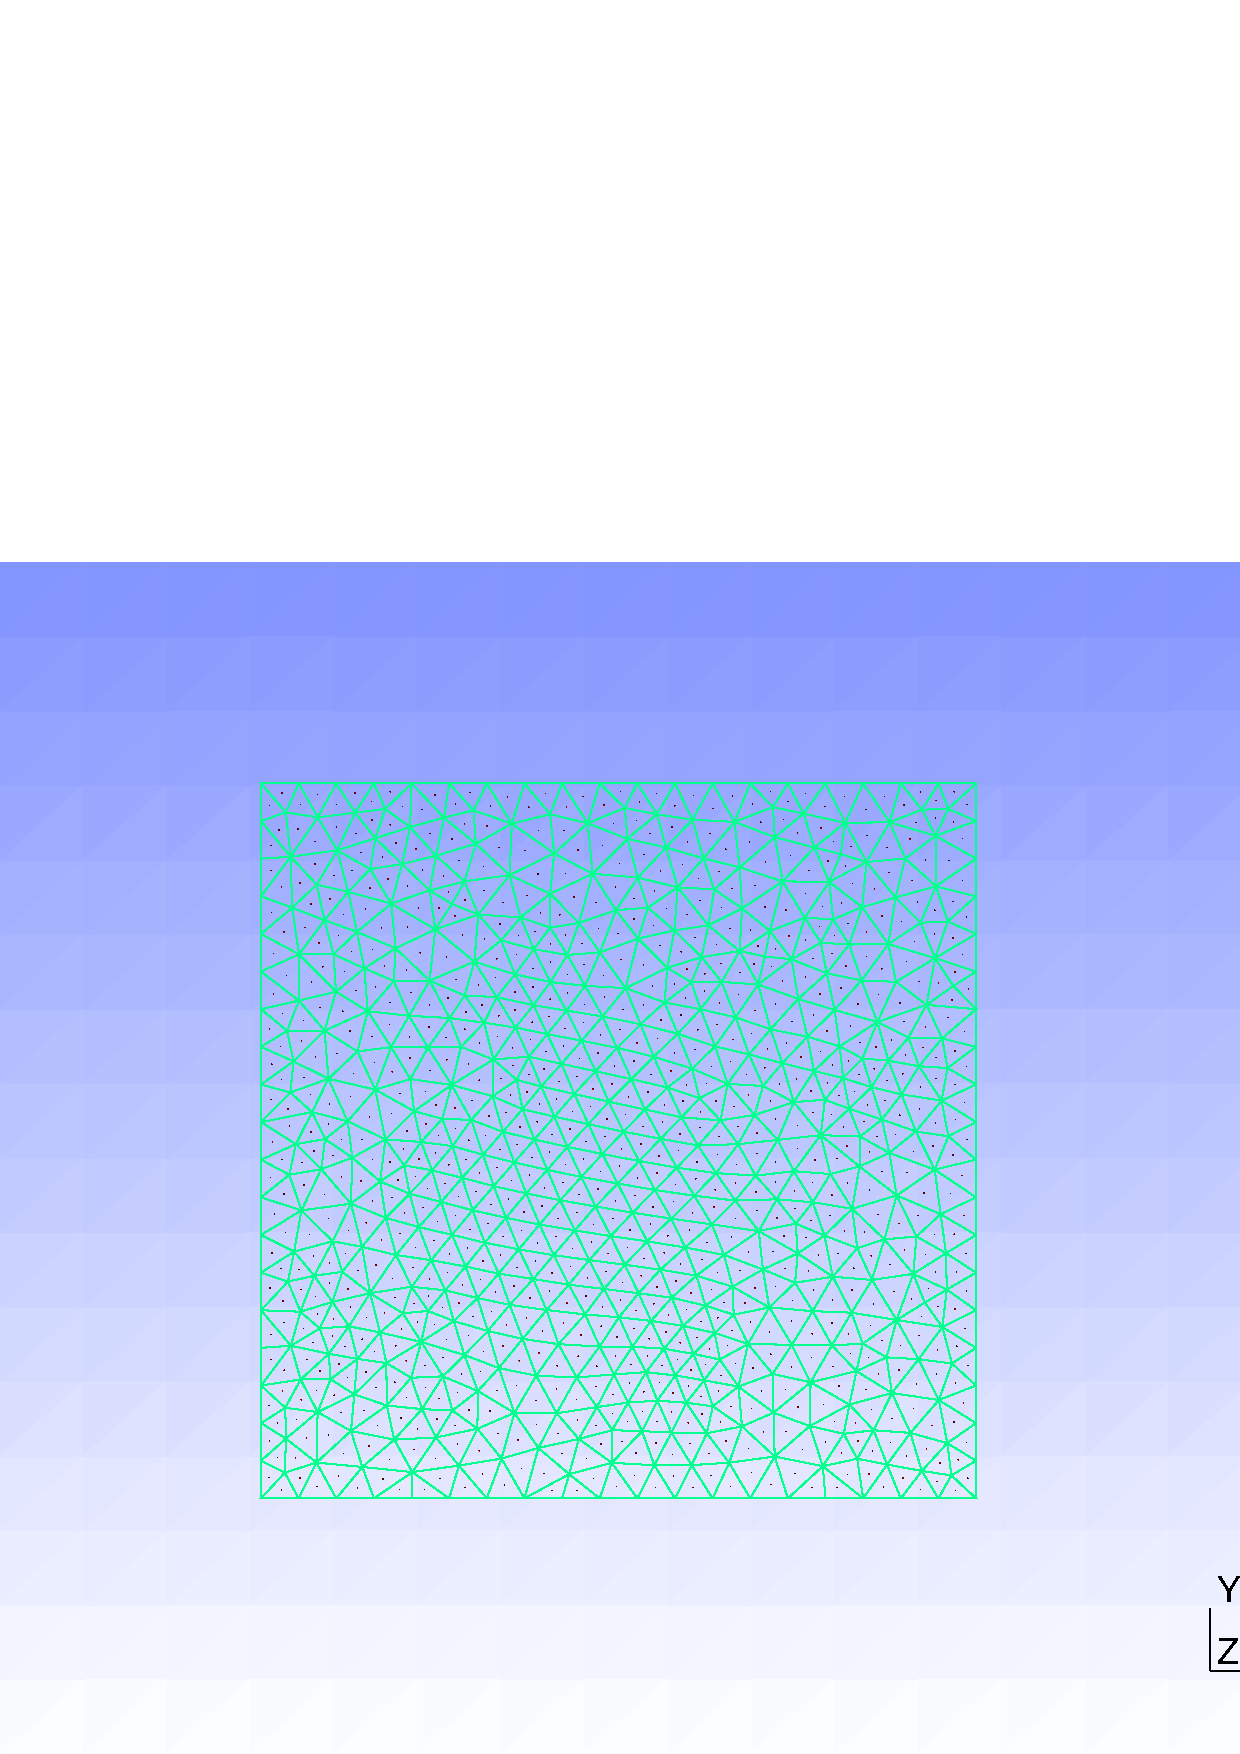
\includegraphics{quad}}
\caption{Quadrilateral with mesh of triangles}
\label{fig:PYCAD 0}
\end{figure}

If you have \gmshextern installed you can run the example and view the
geometry and mesh with:
\begin{verbatim}
run-escript quad.py
gmsh quad.geo
gmsh quad.msh
\end{verbatim}
See Figure~\ref{fig:PYCAD 0} for a result.

In most cases it is best practice to generate the mesh and solve the
mathematical model in two separate scripts. In our example you can read the
\finley mesh into your simulation code\footnote{\gmshextern files can be
directly read using \function{ReadGmsh}, see \Chap{chap:finley}} using
\begin{python}
  from finley import ReadMesh
  mesh=ReadMesh("quad.fly")
\end{python}
Note that the underlying mesh generation software will not accept all
the geometries you can create.  For example, \pycad will happily allow
you to create a 2-D \class{Design} that is a closed loop with some
additional points or lines lying outside of the enclosed area, but
\gmshextern will fail to create a mesh for it.

\section{Holes}
The example included below shows how to use \pycad to create a 2-D mesh
in the shape of a trapezoid with a cut-out area as in Figure~\ref{fig:PYCAD 1}.

\begin{python}
  from esys.pycad import *
  from esys.pycad.gmsh import Design
  from esys.finley import MakeDomain
  
  # A trapezoid
  p0=Point(0.0, 0.0, 0.0)
  p1=Point(1.0, 0.0, 0.0)
  p2=Point(1.0, 0.5, 0.0)
  p3=Point(0.0, 1.0, 0.0)
  l01=Line(p0, p1)
  l12=Line(p1, p2)
  l23=Line(p2, p3)
  l30=Line(p3, p0)
  c=CurveLoop(l01, l12, l23, l30)
  
  # A small triangular cutout
  x0=Point(0.1, 0.1, 0.0)
  x1=Point(0.5, 0.1, 0.0)
  x2=Point(0.5, 0.2, 0.0)
  x01=Line(x0, x1)
  x12=Line(x1, x2)
  x20=Line(x2, x0)
  cutout=CurveLoop(x01, x12, x20)
  
  # Create the surface with cutout
  s=PlaneSurface(c, holes=[cutout])
  
  # Create a Design which can make the mesh
  d=Design(dim=2, element_size=0.05)
  
  # Add the trapezoid with cutout
  d.addItems(s)
  
  # Create the geometry, mesh and Escript domain
  d.setScriptFileName("trapezoid.geo")
  d.setMeshFileName("trapezoid.msh")
  domain=MakeDomain(d)
  # write mesh to a finley file:
  domain.write("trapezoid.fly")
\end{python}
This example is included with the software in \file{trapezoid.py} in the
\ExampleDirectory.

\begin{figure}
\centerline{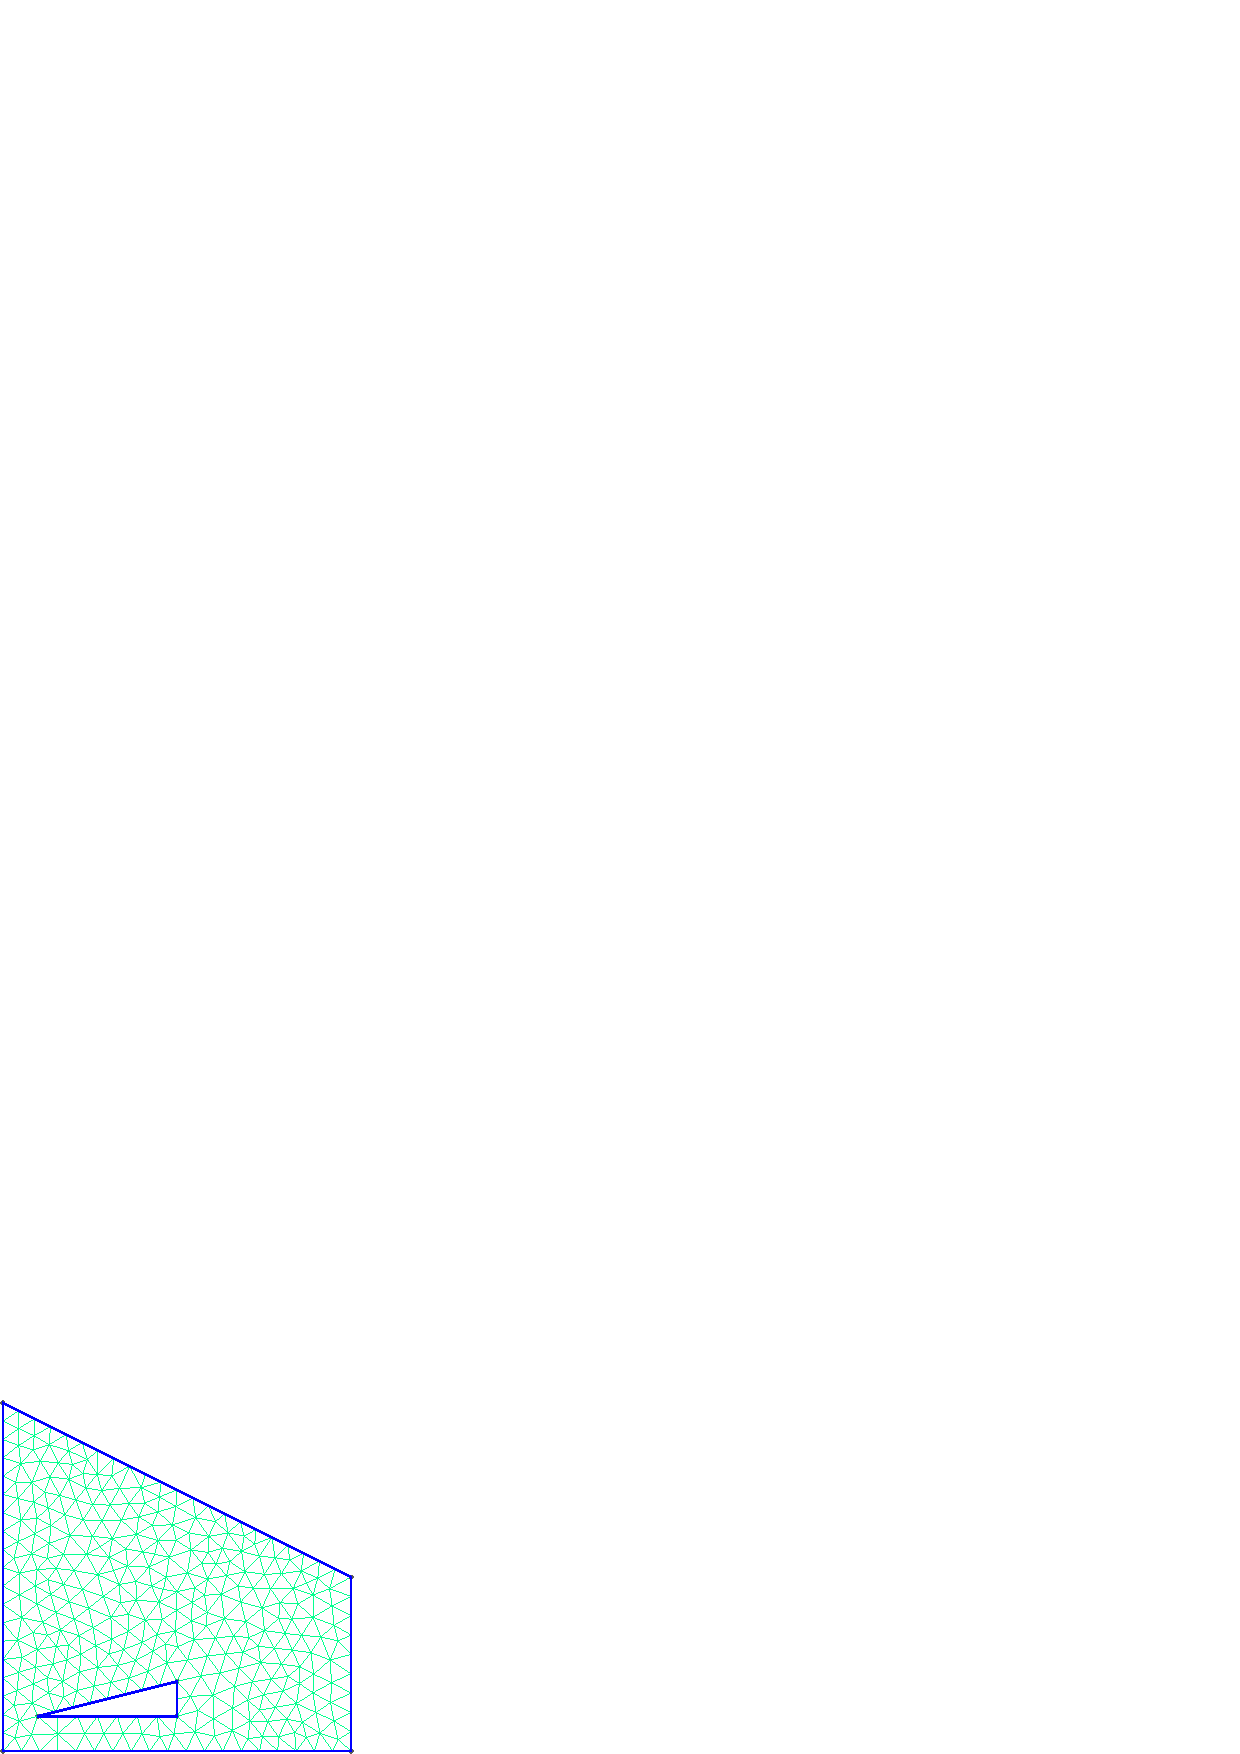
\includegraphics{trapezoid}}
\caption{Trapezoid with triangular hole}
\label{fig:PYCAD 1}
\end{figure}

A \code{CurveLoop} is used to connect several lines into a single curve.
It is used in the example above to create the trapezoidal outline for the grid
and also for the triangular cutout area.
You can define any number of lines when creating a \class{CurveLoop}, but
the end of one line must be identical to the start of the next.

\section{A 3D example}

In this section we discuss the definition of 3D geometries. As an example
consider the unit cube as shown in Figure~\ref{fig:PYCAD 2}.
First we generate the vertices of the cube:
\begin{python}
  from esys.pycad import *
  p0=Point(0.,0.,0.)
  p1=Point(1.,0.,0.)
  p2=Point(0.,1.,0.)
  p3=Point(1.,1.,0.)
  p4=Point(0.,0.,1.)
  p5=Point(1.,0.,1.)
  p6=Point(0.,1.,1.)
  p7=Point(1.,1.,1.)
\end{python}

We connect the points to form the bottom and top surfaces of the cube:
\begin{python}
  l01=Line(p0,p1)
  l13=Line(p1,p3)
  l32=Line(p3,p2)
  l20=Line(p2,p0)
  bottom=PlaneSurface(-CurveLoop(l01,l13,l32,l20))
\end{python}

\begin{figure}
\centerline{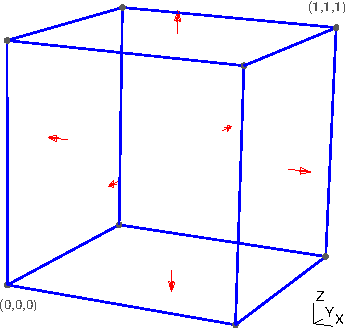
\includegraphics{brick}}
\caption{Three dimensional block}
\label{fig:PYCAD 2}
\end{figure}

Similar to the definition of a \code{CurvedLoop} the orientation of the
surfaces in a \code{SurfaceLoop} is relevant.
In fact, the surface normal direction defined by the right-hand rule needs to
point outwards as indicated by the surface normals in Figure~\ref{fig:PYCAD 2}.
As the \code{bottom} face is directed upwards it is inserted with the minus
sign into the \code{SurfaceLoop} in order to adjust the orientation of the
surface. Similarly we set 
\begin{python}
  l45=Line(p4,p5)
  l57=Line(p5,p7)
  l76=Line(p7,p6)
  l64=Line(p6,p4)
  top=PlaneSurface(CurveLoop(l45,l57,l76,l64))
\end{python}
To form the front face we introduce the two additional lines connecting the
left and right front points of the \code{top} and \code{bottom} face:
\begin{python}
  l15=Line(p1,p5)
  l40=Line(p4,p0)
\end{python}
To form the front face we encounter a problem, the line \code{l45} used
to define the \code{top} face is pointing the wrong direction.
In \pycad you can reverse the direction of an object by changing its sign.
So we write \code{-l45} to indicate that the direction is to be reversed.
With this notation we can write
\begin{python}
  front=PlaneSurface(CurveLoop(l01,l15,-l45,l40))
\end{python}
Keep in mind that if you use \code{Line(p4,p5)} instead of \code{-l45} both
objects are treated as different although connecting the same points with a
straight line in the same direction. The resulting geometry would include an
opening along the \code{p4}--\code{p5} connection.
This will lead to an inconsistent mesh and may result in a failure of the
volumetric mesh generator. Similarly we can define the other sides of the cube:
\begin{python}
  l37=Line(p3,p7)
  l62=Line(p6,p2)
  back=PlaneSurface(CurveLoop(l32,-l62,-l76,-l37))
  left=PlaneSurface(CurveLoop(-l40,-l64,l62,l20))
  right=PlaneSurface(CurveLoop(-l15,l13,l37,-l57))
\end{python}
We can now put the six surfaces together to form a \class{SurfaceLoop}
defining the boundary of the volume of the cube:
\begin{python}
  sl=SurfaceLoop(top,bottom,front,back,left,right)
  v=Volume(sl)
\end{python}
As in the 2D case, the \class{Design} class is used to define the geometry:
\begin{python}
  from esys.pycad.gmsh import Design
  from esys.finley import MakeDomain

  des=Design(dim=3, element_size = 0.1, keep_files=True)
  des.setScriptFileName("brick.geo")
  des.addItems(v, top, bottom, back, front, left, right)

  dom=MakeDomain(des)
  dom.write("brick.fly")
\end{python}
Note that the \finley mesh file \file{brick.fly} will contain the
triangles used to define the surfaces as they are added to the \class{Design}.
The example script of the cube is included with the software in
\file{brick.py} in the \ExampleDirectory.

\section{Alternative File Formats}
\pycad supports other file formats including I-DEAS universal file, VRML,
Nastran and STL. The following example shows how to generate the STL file
\file{brick.stl}:
\begin{python}
  from esys.pycad.gmsh import Design

  des=Design(dim=3, element_size = 0.1, keep_files=True)
  des.addItems(v, top, bottom, back, front, left , right)

  des.setFileFormat(des.STL)
  des.setMeshFileName("brick.stl")
  des.generate()
\end{python}
The example script of the cube is included with the software in
\file{brick_stl.py} in the \ExampleDirectory.

\section{Element Sizes}
The element size used globally is defined by the \code{element_size} argument
of the \class{Design}. The mesh generator will try to use this mesh size
everywhere in the geometry. In some cases it can be desirable to use a finer
mesh locally. A local refinement can be defined at each \class{Point}:
\begin{python}
  p0=Point(0., 0., 0., local_scale=0.01)
\end{python}
Here the mesh generator will create a mesh with an element size which is by
the factor \code{0.01} times smaller than the global mesh size
\code{element_size=0.3}, see Figure~\ref{fig:PYCAD 5}.
The point where a refinement is defined must be a point on a curve used to
define the geometry.

\begin{figure}
\centerline{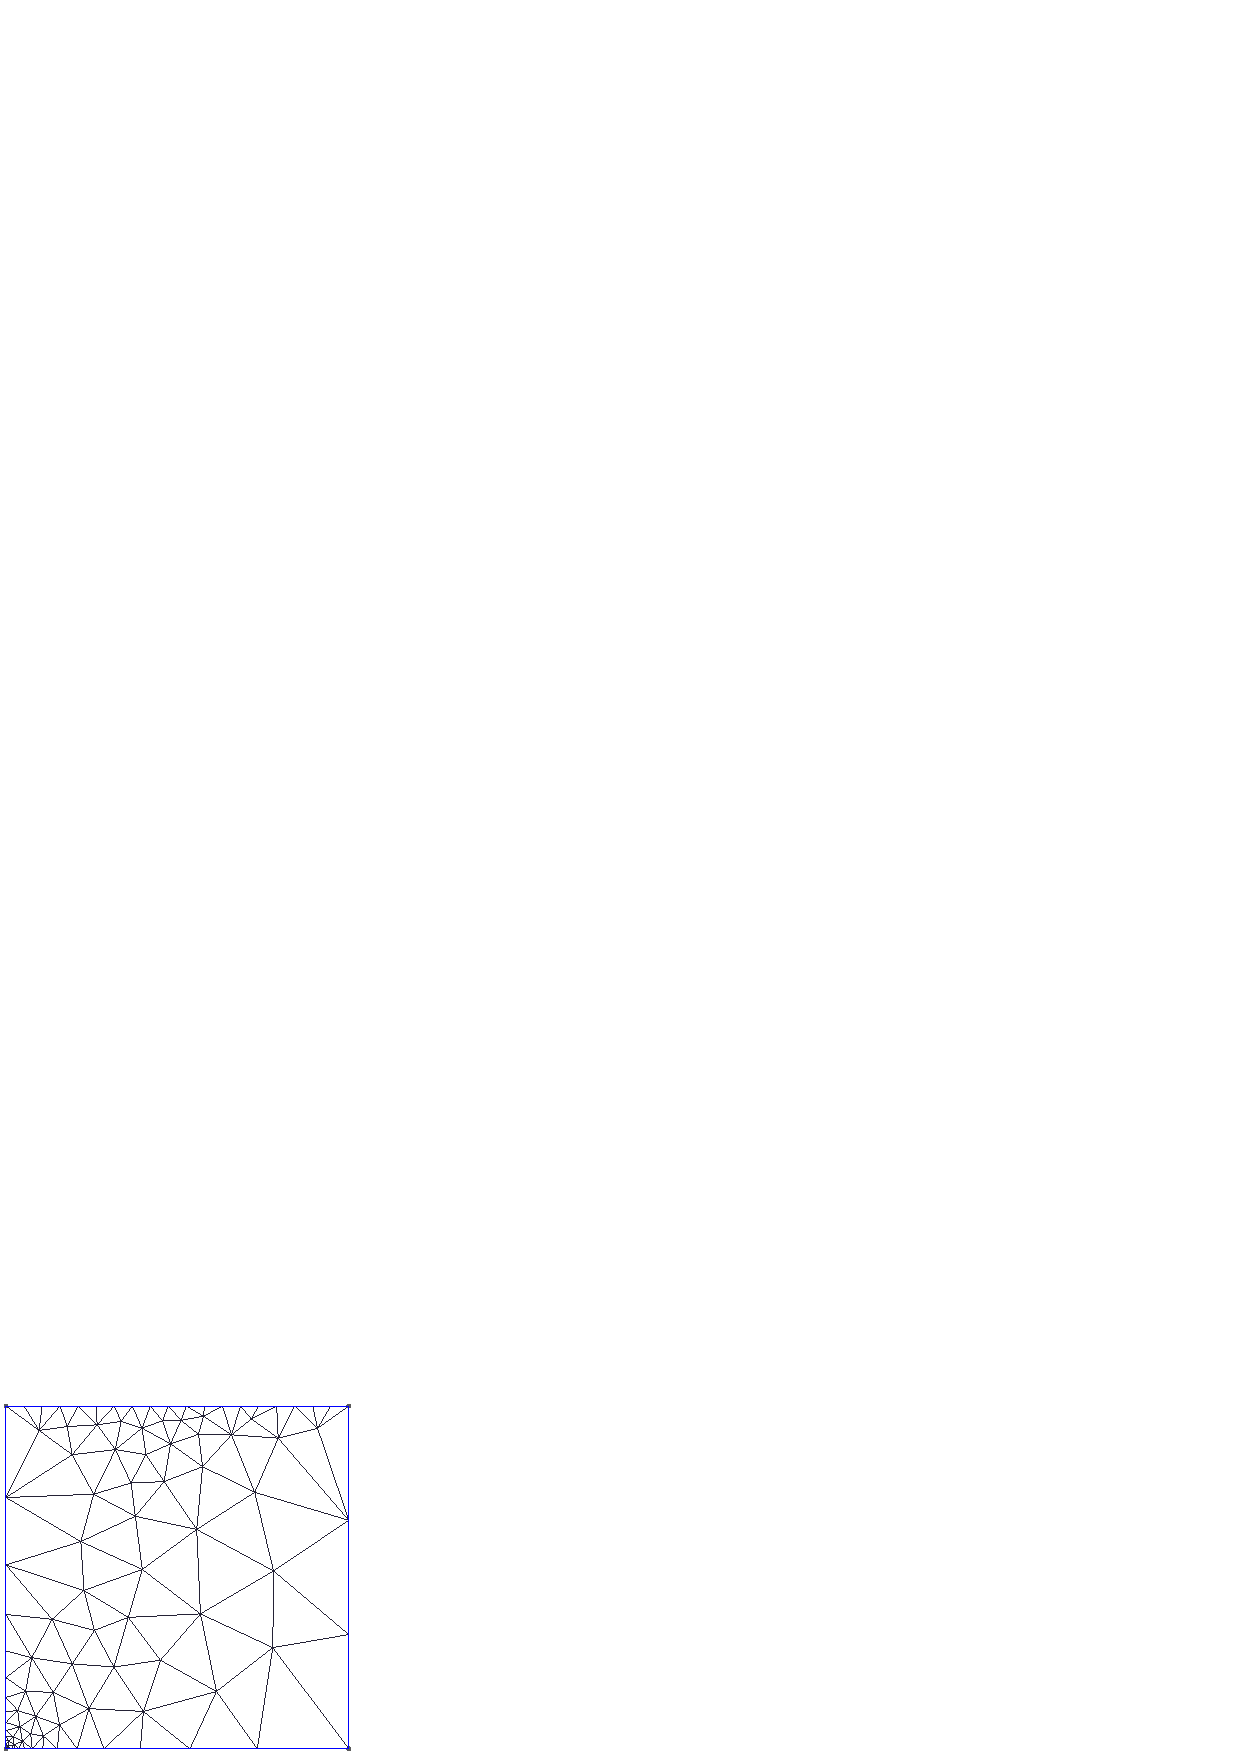
\includegraphics{refine}}
\caption{Local refinement at the origin by \var{local_scale=0.01}
with \var{element_size=0.3} and number of elements on the top set to 10}
\label{fig:PYCAD 5}
\end{figure}

Alternatively, one can define a mesh size along a curve by defining the number
of elements to be used to subdivide the curve. For instance, to use $20$
elements on line \code{l23}:
\begin{python}
  l23=Line(p2, p3)
  l23.setElementDistribution(20)
\end{python}
Setting the number of elements on a curve overwrites the global mesh size
\code{element_size}. The result is shown in Figure~\ref{fig:PYCAD 5}.

\section{\pycad Classes}
%\declaremodule{extension}{esys.pycad}
%\modulesynopsis{Python geometry description and meshing interface}

\subsection{Primitives}
Some of the most commonly-used objects in \pycad are listed here.
For a more complete list see the full API documentation.

\begin{classdesc}{Point}{x=0.,y=0.,z=0.\optional{,local_scale=1.}}
creates a point at the given coordinates with local characteristic length \var{local_scale}
\end{classdesc}

\begin{classdesc}{CurveLoop}{list}
creates a closed curve from a \code{list} of
\class{Line}, \class{Arc}, \class{Spline}, \class{BSpline},
\class{BezierSpline} objects.
\end{classdesc}

\begin{classdesc}{SurfaceLoop}{list}
creates a loop of \class{PlaneSurface} or \class{RuledSurface}, which defines
the shell of a volume.
\end{classdesc}

\subsubsection{Lines}
\begin{classdesc}{Line}{point1, point2}
creates a line between two points.
\end{classdesc}

\begin{methoddesc}[Line]{setElementDistribution}{n\optional{,progression=1\optional{,createBump=\False}}}
defines the number of elements on the line. If set, it overwrites the local
length setting which would be applied.
The progression factor \var{progression} defines the change of element size
between neighboured elements. If \var{createBump} is set progression is
applied towards the centre of the line.
\end{methoddesc}

\begin{methoddesc}[Line]{resetElementDistribution}{}
removes a previously set element distribution from the line.
\end{methoddesc}
\begin{methoddesc}[Line]{getElementDistribution}{}
returns the element distribution as a tuple of number of elements, progression
factor and bump flag. If no element distribution is set None is returned.
\end{methoddesc}

\subsubsection{Splines}
\begin{classdesc}{Spline}{point0, point1, ...}
A spline curve defined by a list of points \var{point0}, \var{point1}, \ldots
\end{classdesc}

\begin{methoddesc}[Spline]{setElementDistribution}{n\optional{,progression=1\optional{,createBump=\False}}}
defines the number of elements on the spline. If set, it overwrites the local
length setting which would be applied.
The progression factor \var{progression} defines the change of element size
between neighboured elements. If \var{createBump} is set progression is
applied towards the centre of the spline.
\end{methoddesc}

\begin{methoddesc}[Spline]{resetElementDistribution}{}
removes a previously set element distribution from the spline.
\end{methoddesc}

\begin{methoddesc}[Spline]{getElementDistribution}{}
returns the element distribution as a tuple of number of elements, progression
factor and bump flag. If no element distribution is set None is returned.
\end{methoddesc}

\subsubsection{BSplines}
\begin{classdesc}{BSpline}{point0, point1, ...}
A B-spline curve defined by a list of points \var{point0}, \var{point1}, \ldots
\end{classdesc}

\begin{methoddesc}[BSpline]{setElementDistribution}{n\optional{,progression=1\optional{,createBump=\False}}}
defines the number of elements on the curve. If set, it overwrites the local
length setting which would be applied.
The progression factor \var{progression} defines the change of element size
between neighboured elements. If \var{createBump} is set progression is
applied towards the centre of the curve.
\end{methoddesc}

\begin{methoddesc}[BSpline]{resetElementDistribution}{}
removes a previously set element distribution from the curve.
\end{methoddesc}

\begin{methoddesc}[BSpline]{getElementDistribution}{}
returns the element distribution as a tuple of number of elements, progression
factor and bump flag. If no element distribution is set None is returned.
\end{methoddesc}

\subsubsection{Bezier Curves}
\begin{classdesc}{BezierCurve}{point0, point1, ...}
A Bezier spline curve defined by a list of points \var{point0}, \var{point1}, \ldots
\end{classdesc}

\begin{methoddesc}[BezierCurve]{setElementDistribution}{n\optional{,progression=1\optional{,createBump=\False}}}
defines the number of elements on the curve. If set, it overwrites the local
length setting which would be applied.
The progression factor \var{progression} defines the change of element size
between neighboured elements. If \var{createBump} is set progression is
applied towards the centre of the curve.
\end{methoddesc}

\begin{methoddesc}[BezierCurve]{resetElementDistribution}{}
removes a previously set element distribution from the curve.
\end{methoddesc}

\begin{methoddesc}[BezierCurve]{getElementDistribution}{}
returns the element distribution as a tuple of number of elements, progression
factor and bump flag. If no element distribution is set None is returned.
\end{methoddesc}

\subsubsection{Arcs}
\begin{classdesc}{Arc}{centre_point, start_point, end_point}
creates an arc by specifying a centre for a circle and start and end points.
An arc may subtend an angle of at most $\pi$ radians.
\end{classdesc}

\begin{methoddesc}[Arc]{setElementDistribution}{n\optional{,progression=1\optional{,createBump=\False}}}
defines the number of elements on the arc. If set, it overwrites the local
length setting which would be applied.
The progression factor \var{progression} defines the change of element size
between neighboured elements. If \var{createBump} is set progression is
applied towards the centre of the arc.
\end{methoddesc}

\begin{methoddesc}[Arc]{resetElementDistribution}{}
removes a previously set element distribution from the arc.
\end{methoddesc}

\begin{methoddesc}[Arc]{getElementDistribution}{}
returns the element distribution as a tuple of number of elements, progression
factor and bump flag. If no element distribution is set None is returned.
\end{methoddesc}

\subsubsection{Plane surfaces}
\begin{classdesc}{PlaneSurface}{loop, \optional{holes=[list]}}
creates a plane surface from a \class{CurveLoop}, which may have one or more
holes described by a \var{list} of \class{CurveLoop} objects.
\end{classdesc}

\begin{methoddesc}[PlaneSurface]{setElementDistribution}{n\optional{,progression=1\optional{,createBump=\False}}}
defines the number of elements on all lines.
\end{methoddesc}

\begin{methoddesc}[PlaneSurface]{setRecombination}{\optional{max_deviation=45 * \var{DEG} }}
the mesh generator will try to recombine triangular elements into
quadrilateral elements. \var{max_deviation} (in radians) defines the
maximum deviation of any angle in the quadrilaterals from the right angle.
Set \var{max_deviation}=\var{None} to remove recombination.
\end{methoddesc}

\begin{methoddesc}[PlaneSurface]{setTransfiniteMeshing}{\optional{orientation="Left"}}
applies 2D transfinite meshing to the surface.
\var{orientation} defines the orientation of triangles. Allowed values
are \var{``Left''}, \var{``Right''} and \var{``Alternate''}.
The boundary of the surface must be defined by three or four lines and an
element distribution must be defined on all faces where opposite
faces use the same element distribution. No holes must be present.
\end{methoddesc}

\subsubsection{Ruled Surfaces}
\begin{classdesc}{RuledSurface}{list}
creates a surface that can be interpolated using transfinite interpolation.
\var{list} gives a list of three or four lines defining the boundary of the
surface.
\end{classdesc}

\begin{methoddesc}[RuledSurface]{setRecombination}{\optional{max_deviation=45 * \var{DEG} }}
the mesh generator will try to recombine triangular elements into
quadrilateral elements. \var{max_deviation} (in radians) defines the
maximum deviation of any angle in the quadrilaterals from the right angle.
Set \var{max_deviation}=\var{None} to remove recombination.
\end{methoddesc}

\begin{methoddesc}[RuledSurface]{setTransfiniteMeshing}{\optional{orientation="Left"}}
applies 2D transfinite meshing to the surface.
\var{orientation} defines the orientation of triangles. Allowed values
are \var{``Left''}, \var{``Right''} and \var{``Alternate''}.
The boundary of the surface must be defined by three or four lines and an
element distribution must be defined on all faces where opposite
faces use the same element distribution. No holes must be present.
\end{methoddesc}

\begin{methoddesc}[RuledSurface]{setElementDistribution}{n\optional{,progression=1\optional{,createBump=\False}}}
defines the number of elements on all lines.
\end{methoddesc}

\subsubsection{Volumes}
\begin{classdesc}{Volume}{loop, \optional{holes=[list]}}
creates a volume given a \class{SurfaceLoop}, which may have one or more holes
define by the list of \class{SurfaceLoop}.
\end{classdesc}

\begin{methoddesc}[Volume]{setElementDistribution}{n\optional{,progression=1\optional{,createBump=\False}}}
defines the number of elements on all lines.
\end{methoddesc}

\begin{methoddesc}[Volume]{setRecombination}{\optional{max_deviation=45 * \var{DEG} }}
the mesh generator will try to recombine triangular elements into
quadrilateral elements. These meshes are then used to generate the volume mesh
if possible.
Together with transfinite meshing one can construct rectangular meshes.
\var{max_deviation} (in radians) defines the maximum deviation of any angle in
the quadrilaterals from the right angle.
Set \var{max_deviation}=\var{None} to remove recombination.
\end{methoddesc}

\begin{methoddesc}[Volume]{setTransfiniteMeshing}{\optional{orientation="Left"}}
applies transfinite meshing to the volume and all surfaces (if
\var{orientation} is not equal to \var{None}).
\var{orientation} defines the orientation of triangles. Allowed values
are \var{``Left''}, \var{``Right''} and \var{``Alternate''}.
The boundary of the surface must be defined by three or four lines and an
element distribution must be defined on all faces where opposite
faces use the same element distribution.
If \var{orientation} is equal to \var{None} transfinite meshing is not
switched on for the surfaces but needs to be set by the user.
No holes must be present.
\textbf{Warning: The functionality of transfinite meshing without
recombination is not entirely clear in \gmshextern.
So please apply this method with care.}
\end{methoddesc}

%============================================================================
\subsection{Transformations}

Sometimes it is convenient to create an object and then make copies at
different orientations or in different sizes. This can be achieved by
applying transformations which are used to move geometrical objects in the
3-dimensional space and to resize them.

\begin{classdesc}{Translation}{\optional{b=[0,0,0]}}
defines a translation $x \to x+b$. \var{b} can be any object that can be
converted into a \numpy object of shape $(3,)$.
\end{classdesc}

\begin{classdesc}{Rotation}{\optional{axis=[1,1,1], \optional{ point = [0,0,0], \optional{angle=0*RAD} } } }
defines a rotation by \var{angle} around axis through point \var{point} and direction \var{axis}.
\var{axis} and \var{point} can be any object that can be converted into a
\numpy object of shape $(3,)$.
\var{axis} does not have to be normalised but must have positive length.
The right-hand rule~\cite{RIGHTHANDRULE} applies.
\end{classdesc}

\begin{classdesc}{Dilation}{\optional{factor=1., \optional{centre=[0,0,0]}}}
defines a dilation by the expansion/contraction \var{factor} with
\var{centre} as the dilation centre.
\var{centre} can be any object that can be converted into a \numpy object of
shape $(3,)$.
\end{classdesc}

\begin{classdesc}{Reflection}{\optional{normal=[1,1,1], \optional{offset=0}}}
defines a reflection on a plane defined in normal form $n^t x = d$
where $n$ is the surface normal \var{normal} and $d$ is the plane \var{offset}.
\var{normal} can be any object that can be converted into a \numpy object of
shape $(3,)$.
\var{normal} does not have to be normalised but must have positive length.
\end{classdesc}

\begin{datadesc}{DEG}
a constant to convert from degrees to an internal angle representation in
radians. For instance use \code{90*DEG} for $90$ degrees.
\end{datadesc}

\subsection{Properties}
If you are building a larger geometry you may find it convenient to
create it in smaller pieces and then assemble them.
Property Sets make this easy, and they allow you to name the smaller
pieces for convenience.

Property Sets are used to bundle a set of geometrical objects in a
group. The group is identified by a name. Typically a Property Set
is used to mark subregions which share the same material properties or
to mark portions of the boundary. For efficiency, the \Design class
assigns an integer to each of its Property Sets, a so-called tag\index{tag}.
The appropriate tag is attached to the elements at generation time.

See the file \code{pycad/examples/quad.py} for an example using a {\it PropertySet}.

\begin{classdesc}{PropertySet}{name,*items}
defines a group geometrical objects which can be accessed through a \var{name}
The objects in the tuple \var{items} mast all be \ManifoldOneD, \ManifoldTwoD or \ManifoldThreeD objects.
\end{classdesc}

\begin{methoddesc}[PropertySet]{getManifoldClass}{}
returns the manifold class \ManifoldOneD, \ManifoldTwoD or \ManifoldThreeD
expected from the items in the property set.
\end{methoddesc}

\begin{methoddesc}[PropertySet]{getDim}{}
returns the spatial dimension of the items in the property set.
\end{methoddesc}

\begin{methoddesc}[PropertySet]{getName}{}
returns the name of the set
\end{methoddesc}

\begin{methoddesc}[PropertySet]{setName}{name}
sets the name. This name should be unique within a \Design.
\end{methoddesc}

\begin{methoddesc}[PropertySet]{addItem}{*items}
adds a tuple of items. They need to be objects of class \ManifoldOneD,
\ManifoldTwoD or \ManifoldThreeD.
\end{methoddesc}

\begin{methoddesc}[PropertySet]{getItems}{}
returns the list of items
\end{methoddesc}

\begin{methoddesc}[PropertySet]{clearItems}{}
clears the list of items
\end{methoddesc}

\begin{methoddesc}[PropertySet]{getTag}{}
returns the tag used for this property set
\end{methoddesc}

\section{Interface to the mesh generation software}
%\declaremodule{extension}{esys.pycad.gmsh}
%\modulesynopsis{Python geometry description and meshing interface}

The class and methods described here provide an interface to the mesh
generation software, which is currently \gmshextern. This interface could be
adopted to \emph{triangle} or another mesh generation package if this is
deemed to be desirable in the future.

\begin{classdesc}{Design}{
\optional{dim=3, \optional{element_size=1., \optional{order=1, \optional{keep_files=False}}}}}
describes the geometry defined by primitives to be meshed.
\var{dim} specifies the spatial dimension, while \var{element_size} defines
the global element size which is multiplied by the local scale to set the
element size at each \Point.
The argument \var{order} defines the element order to be used.
If \var{keep_files} is set to \True temporary files are kept, otherwise they
are removed when the instance of the class is deleted.
\end{classdesc}

\begin{memberdesc}[Design]{GMSH}
gmsh file format~\cite{GMSH}
\end{memberdesc}

\begin{memberdesc}[Design]{IDEAS}
I-DEAS universal file format~\cite{IDEAS}
\end{memberdesc}

\begin{memberdesc}[Design]{VRML}
VRML file format, \cite{VRML}
\end{memberdesc}

\begin{memberdesc}[Design]{STL}
STL file format~\cite{STL}
\end{memberdesc}

\begin{memberdesc}[Design]{NASTRAN}
NASTRAN bulk data format~\cite{NASTRAN}
\end{memberdesc}

\begin{memberdesc}[Design]{MEDIT}
Medit file format~\cite{MEDIT}
\end{memberdesc}

\begin{memberdesc}[Design]{CGNS}
CGNS file format~\cite{CGNS}
\end{memberdesc}

\begin{memberdesc}[Design]{PLOT3D}
Plot3D file format~\cite{PLOT3D}
\end{memberdesc}

\begin{memberdesc}[Design]{DIFFPACK}
Diffpack 3D file format~\cite{DIFFPACK}
\end{memberdesc}

\begin{memberdesc}[Design]{DELAUNAY}
the Delaunay triangulator, see \gmshextern and \cite{TETGEN}
\end{memberdesc}

\begin{memberdesc}[Design]{MESHADAPT}
the gmsh triangulator, see \gmshextern
\end{memberdesc}

\begin{memberdesc}[Design]{FRONTAL}
the NETGEN~\cite{NETGEN} triangulator
\end{memberdesc}

\begin{methoddesc}[Design]{generate}{}
generates the mesh file. The data are written to the file \var{Design.getMeshFileName}.
\end{methoddesc}

\begin{methoddesc}[Design]{setDim}{\optional{dim=3}}
sets the spatial dimension which needs to be $1$, $2$ or $3$.
\end{methoddesc}

\begin{methoddesc}[Design]{getDim}{}
returns the spatial dimension.
\end{methoddesc}

\begin{methoddesc}[Design]{setElementOrder}{\optional{order=1}}
sets the element order which needs to be $1$ or $2$.
\end{methoddesc}

\begin{methoddesc}[Design]{getElementOrder}{}
returns the element order.
\end{methoddesc}

\begin{methoddesc}[Design]{setElementSize}{\optional{element_size=1}}
sets the global element size. The local element size at a point is defined as
the global element size multiplied by the local scale.
The element size must be positive.
\end{methoddesc}

\begin{methoddesc}[Design]{getElementSize}{}
returns the global element size.
\end{methoddesc}

\begin{methoddesc}[Design]{setKeepFilesOn}{}
work files are kept at the end of the generation.
\end{methoddesc}

\begin{methoddesc}[Design]{setKeepFilesOff}{}
work files are deleted at the end of the generation.
\end{methoddesc}

\begin{methoddesc}[Design]{keepFiles}{}
returns \True if work files are kept, \False otherwise.
\end{methoddesc}

\begin{methoddesc}[Design]{setScriptFileName}{\optional{name=None}}
sets the file name for the gmsh input script.
If no name is given a name with extension "geo" is generated.
\end{methoddesc}

\begin{methoddesc}[Design]{getScriptFileName}{}
returns the name of the file for the gmsh script.
\end{methoddesc}

\begin{methoddesc}[Design]{setMeshFileName}{\optional{name=None}}
sets the name for the mesh file. If no name is given a name is generated.
The format is set by \\\var{Design.setFileFormat}.
\end{methoddesc}

\begin{methoddesc}[Design]{getMeshFileName}{}
returns the name of the mesh file.
\end{methoddesc}

\begin{methoddesc}[Design]{addItems}{*items}
adds the tuple of \var{items}. An item can be any primitive or a
\class{PropertySet}.
\warning{If a \PropertySet is added which includes an object that is not
part of a \PropertySet, it may not be considered in the meshing.}
\end{methoddesc}

\begin{methoddesc}[Design]{getItems}{}
returns a list of the items.
\end{methoddesc}

\begin{methoddesc}[Design]{clearItems}{}
resets the items in this design.
\end{methoddesc}

\begin{methoddesc}[Design]{getMeshHandler}{}
returns a handle to the mesh.
Calling this method generates the mesh from the geometry and returns a
mechanism to access the mesh data. In the current implementation this
method returns a file name for a file containing the mesh data.
\end{methoddesc}

\begin{methoddesc}[Design]{getScriptString}{}
returns the gmsh script to generate the mesh as a string.
\end{methoddesc}

\begin{methoddesc}[Design]{getCommandString}{}
returns the gmsh command used to generate the mesh as a string.
\end{methoddesc}

\begin{methoddesc}[Design]{setOptions}{
\optional{algorithm=None
\optional{, optimize_quality=\True
\optional{, smoothing=1
\optional{, curvature_based_element_size=\False
\optional{, algorithm2D=None
\optional{, algorithm3D=None
\optional{, generate_hexahedra=False
\optional{, random_factor=None}}}}}}}}}
sets options for the mesh generator.
Both \var{algorithm} and \var{algorithm2D} set the 2D meshing algorithm to be
used. If both parameters are given, they must be equal.
The algorithm needs to be \var{Design.DELAUNAY}, \var{Design.FRONTAL},
or \var{Design.MESHADAPT}. By default \var{Design.MESHADAPT} is used.
\var{algorithm3D} sets the 3D  meshing algorithm to be used.
The algorithm needs to be \var{Design.DELAUNAY} or \var{Design.FRONTAL}.
By default \var{Design.FRONTAL} is used.
\var{optimize_quality}=\True invokes an optimization of the mesh quality.
\var{smoothing} sets the number of smoothing steps to be applied to the mesh.
\var{curvature_based_element_size}=\True switches on curvature based
definition of element size.
\var{generate_hexahedra}=\True switches on the usage of quadrilateral or
hexahedral elements.
\var{random_factor} a positive amount used in the 2D meshing algorithm.
\end{methoddesc}

\begin{methoddesc}[Design]{getTagMap}{}
returns a \class{TagMap} to map the \class{PropertySet} names to tag numbers
generated by gmsh.
\end{methoddesc}

\begin{methoddesc}[Design]{setFileFormat}{\optional{format=\var{Design.GMSH}}}
sets the file format. \var{format} must be one of the values:\\
\var{Design.GMSH}\\
\var{Design.IDEAS}\\
\var{Design.VRML}\\
\var{Design.STL}\\
\var{Design.NASTRAN}\\
\var{Design.MEDIT}\\
\var{Design.CGNS}\\
\var{Design.PLOT3D}\\
\var{Design.DIFFPACK}.
\end{methoddesc}

\begin{methoddesc}[Design]{getFileFormat}{}
returns the file format.
\end{methoddesc}




%%%%%%%%%%%%%%%%%%%%%%%%%%%%%%%%%%%%%%%%%%%%%%%%%%%%%%%%
%
% Copyright (c) 2003-2008 by University of Queensland
% Earth Systems Science Computational Center (ESSCC)
% http://www.uq.edu.au/esscc
%
% Primary Business: Queensland, Australia
% Licensed under the Open Software License version 3.0
% http://www.opensource.org/licenses/osl-3.0.php
%
%%%%%%%%%%%%%%%%%%%%%%%%%%%%%%%%%%%%%%%%%%%%%%%%%%%%%%%%


\chapter{The Module \pyvisi}
\label{PYVISI CHAP}
\declaremodule{extension}{esys.pyvisi}
\modulesynopsis{Python Visualization Interface}

\begin{Large}\strong{Warning: The Module \pyvisi is no longer supported and will be removed from future releases.}\end{Large}


\strong{\begin{Large}Warning: The Module \pyvisi is not supported under MPI        \end{Large}.}

\section{Introduction}
\pyvisi is a Python module that is used to generate 2D and 3D visualizations 
for escript and its PDE solver finley. The module provides 
an easy to use interface to the \VTK library (\VTKUrl) to render (generate)
surface maps and contours for scalar fields, arrows and streamlines for vector
fields, and ellipsoids for tensor fields. There are three approaches for
rendering an object. (1) Online - object is rendered on-screen with
interaction capability (i.e. zoom and rotate), (2) Offline - object is
rendered off-screen (no pop-up window) and (3) Display - object is rendered
on-screen but with no interaction capability (on-the-fly animation). All three
approaches have the option to save the rendered object as an image (e.g. jpeg)
and subsequently converting a series of images into a movie (mpeg).

The following outlines the general steps to use Pyvisi:

\begin{enumerate}
\item Create a \Scene instance - a window in which objects will be rendered on.
\item Create a data input instance (i.e. \DataCollector or \ImageReader) - 
reads the source data for visualization.
\item Create a data visualization object (i.e. \Map, \Velocity, \Ellipsoid, 
\Contour, \Carpet, \StreamLine, etc.) - creates a visual representation of
the source data.
\item Create a \Camera or \Light instance - controls the viewing angle and
lighting effects.
\item Render the object - using either the Online, Offline or Display approach.
\item Generate movie - converts a series of images into a movie. (optional)
\end{enumerate}
\begin{center}
\begin{math}
scene \rightarrow data \; input \rightarrow data \; visualization \rightarrow 
camera \, / \, light \rightarrow render \rightarrow movie
\end{math}
\end{center}

\section{\pyvisi Classes}
The following subsections give a brief overview of the important classes 
and some of their corresponding methods. Please refer to \ReferenceGuide for 
full details.


%#############################################################################


\subsection{Scene Classes}
This section details the instances used to setup the viewing environment.

\subsubsection{\Scene class}

\begin{classdesc}{Scene}{renderer = Renderer.ONLINE, num_viewport = 1, 
x_size = 1152, y_size = 864}
A scene is a window in which objects are to be rendered on. Only 
one scene needs to be created. However, a scene may be divided into four 
smaller windows called viewports (if needed). Each viewport in turn can 
render a different object. 
\end{classdesc}

The following are some of the methods available:
\begin{methoddesc}[Scene]{setBackground}{color}
Set the background color of the scene.
\end{methoddesc}

\begin{methoddesc}[Scene]{render}{image_name = None}
Render the object using either the Online, Offline or Display mode.
\end{methoddesc}

\subsubsection{\Camera class}

\begin{classdesc}{Camera}{scene, viewport = Viewport.SOUTH_WEST}
A camera controls the display angle of the rendered object and one is 
usually created for a \Scene. However, if a \Scene has four viewports, then a 
separate camera may be created for each viewport. 
\end{classdesc}

The following are some of the methods available:
\begin{methoddesc}[Camera]{setFocalPoint}{position}
Set the focal point of the camera.
\end{methoddesc}

\begin{methoddesc}[Camera]{setPosition}{position}
Set the position of the camera.
\end{methoddesc}

\begin{methoddesc}[Camera]{azimuth}{angle}
Rotate the camera to the left and right. The angle parameter is in degrees.
\end{methoddesc}

\begin{methoddesc}[Camera]{elevation}{angle}
Rotate the camera up and down (angle must be between -90 and 90).
\end{methoddesc}

\begin{methoddesc}[Camera]{backView}{}
Rotate the camera to view the back of the rendered object.
\end{methoddesc}

\begin{methoddesc}[Camera]{topView}{}
Rotate the camera to view the top of the rendered object.
\end{methoddesc}

\begin{methoddesc}[Camera]{bottomView}{}
Rotate the camera to view the bottom of the rendered object.
\end{methoddesc}

\begin{methoddesc}[Camera]{leftView}{}
Rotate the camera to view the left side of the rendered object.
\end{methoddesc}

\begin{methoddesc}[Camera]{rightView}{}
Rotate the camera to view the right side of the rendered object.
\end{methoddesc}

\begin{methoddesc}[Camera]{isometricView}{}
Rotate the camera to view an isometric projection of the rendered object.
\end{methoddesc}

\begin{methoddesc}[Camera]{dolly}{distance}
Move the camera towards (greater than 1) the rendered object. However,
it is not possible to move the camera away from the rendered object with this
method.
\end{methoddesc}

\subsubsection{\Light class}

\begin{classdesc}{Light}{scene, viewport = Viewport.SOUTH_WEST}
A light controls the lighting effect for the rendered object and is set up in 
a similar way to \Camera.
\end{classdesc}

The following are some of the methods available:
\begin{methoddesc}[Light]{setColor}{color}
Set the light color.
\end{methoddesc}

\begin{methoddesc}[Light]{setFocalPoint}{position}
Set the focal point of the light.
\end{methoddesc}

\begin{methoddesc}[Light]{setPosition}{position}
Set the position of the light.
\end{methoddesc}

\begin{methoddesc}[Light]{setAngle}{elevation = 0, azimuth = 0}
An alternative to set the position and focal point of the light by using
elevation and azimuth.
\end{methoddesc}


%##############################################################################


\subsection{Input Classes}
\label{INPUT SEC}
This subsection details the instances used to read and load the source data
for visualization.

\subsubsection{\DataCollector class}
\begin{classdesc}{DataCollector}{source = Source.XML}
A data collector is used to read data either from an XML file (using 
\texttt{setFileName()}) or from an escript object directly (using 
\texttt{setData()}). Writing XML files is expensive but has the advantage
that the results can be analyzed easily after the simulation has completed.   
\end{classdesc}

The following are some of the methods available:
\begin{methoddesc}[DataCollector]{setFileName}{file_name}
Set the XML file name to read.
\end{methoddesc}

\begin{methoddesc}[DataCollector]{setData}{**args}
Create data using the \textless name\textgreater=\textless data\textgreater 
pairing. The method assumes that the data is given in the appropriate format.
\end{methoddesc}

\begin{methoddesc}[DataCollector]{setActiveScalar}{scalar}
Specify the scalar field to load.
\end{methoddesc}

\begin{methoddesc}[DataCollector]{setActiveVector}{vector}
Specify the vector field to load.
\end{methoddesc}

\begin{methoddesc}[DataCollector]{setActiveTensor}{tensor}
Specify the tensor field to load.
\end{methoddesc}

\subsubsection{\ImageReader class}

\begin{classdesc}{ImageReader}{format}
An image reader is used to read data from an image in a variety of formats.
\end{classdesc}

The following is one of the methods available:
\begin{methoddesc}[ImageReader]{setImageName}{image_name}
Set the filename of the image to be loaded.
\end{methoddesc}

\subsubsection{\TextTwoD class}

\begin{classdesc}{Text2D}{scene, text, viewport = Viewport.SOUTH_WEST}
This class is used to insert two-dimensional text for annotations
(e.g. titles, authors and labels).
\end{classdesc}

The following are some of the methods available:
\begin{methoddesc}[Text2D]{setFontSize}{size}
Set the 2D text size.
\end{methoddesc}

\begin{methoddesc}[Text2D]{boldOn}{}
Use bold font style for the text.
\end{methoddesc}

\begin{methoddesc}[Text2D]{setColor}{color}
Set the color of the 2D text.
\end{methoddesc}

Including methods from \ActorTwoD. 


%##############################################################################


\subsection{Data Visualization Classes}
\label{DATAVIS SEC}
This subsection details the instances used to process and manipulate the source
data. The typical usage of some of the classes is also shown. See \Sec{SAMPLEOUTPUT SEC} for sample images generated with these classes.

One point to note is that the source can either be point or cell data. If the
source is cell data, a conversion to point data may or may not be
required, in order for the object to be rendered correctly.
If a conversion is needed, the 'cell_to_point' flag (see below) must 
be set to 'True', otherwise to 'False' (which is the default). On occasions, an
inaccurate object may be rendered from cell data even after conversion.

\subsubsection{\Map class}

\begin{classdesc}{Map}{scene, data_collector, 
viewport = Viewport.SOUTH_WEST, lut = Lut.COLOR, cell_to_point = False,
outline = True}
Class that shows a scalar field on a domain surface. The domain surface 
can either be color or gray-scale, depending on the lookup table used.
\end{classdesc}

The following are some of the methods available:\\
Methods from \ActorThreeD and \DataSetMapper.

A typical usage of \Map is shown below.

\begin{python}
"""
Author: John Ngui, john.ngui@uq.edu.au
"""

# Import the necessary modules.
from esys.pyvisi import Scene, DataCollector, Map, Camera
from esys.pyvisi.constant import *
import os

PYVISI_EXAMPLE_MESHES_PATH = "data_meshes"
PYVISI_EXAMPLE_IMAGES_PATH = "data_sample_images"
X_SIZE = 800
Y_SIZE = 800

SCALAR_FIELD_POINT_DATA = "temperature"
SCALAR_FIELD_CELL_DATA = "temperature_cell"
FILE_3D = "interior_3D.xml"
IMAGE_NAME = "map.jpg"
JPG_RENDERER = Renderer.ONLINE_JPG

# Create a Scene with four viewports.
s = Scene(renderer = JPG_RENDERER, num_viewport = 4, x_size = X_SIZE, 
        y_size = Y_SIZE)

# Create a DataCollector reading from a XML file.
dc1 = DataCollector(source = Source.XML)
dc1.setFileName(file_name = os.path.join(PYVISI_EXAMPLE_MESHES_PATH, FILE_3D))
dc1.setActiveScalar(scalar = SCALAR_FIELD_POINT_DATA)

# Create a  Map for the first viewport.
m1 = Map(scene = s, data_collector = dc1, viewport = Viewport.SOUTH_WEST, 
        lut = Lut.COLOR, cell_to_point = False, outline = True)
m1.setRepresentationToWireframe()

# Create a Camera for the first viewport
c1 = Camera(scene = s, viewport = Viewport.SOUTH_WEST)
c1.isometricView()

# Create a second DataCollector reading from the same XML file but specifying
# a different scalar field.
dc2 = DataCollector(source = Source.XML)
dc2.setFileName(file_name = os.path.join(PYVISI_EXAMPLE_MESHES_PATH, FILE_3D))
dc2.setActiveScalar(scalar = SCALAR_FIELD_CELL_DATA)

# Create a Map for the third viewport.
m2 = Map(scene = s, data_collector = dc2, viewport = Viewport.NORTH_EAST, 
        lut = Lut.COLOR, cell_to_point = True, outline = True)

# Create a Camera for the third viewport
c2 = Camera(scene = s, viewport = Viewport.NORTH_EAST)

# Render the object.
s.render(image_name = os.path.join(PYVISI_EXAMPLE_IMAGES_PATH, IMAGE_NAME))
\end{python}

\subsubsection{\MapOnPlaneCut class}

\begin{classdesc}{MapOnPlaneCut}{scene, data_collector, 
viewport = Viewport.SOUTH_WEST, lut = Lut.COLOR, cell_to_point = False, 
outline = True}
This class works in a similar way to \Map, except that the result is a slice of
the scalar field produced by cutting the map with a plane. The plane can be
translated and rotated to its desired position.
\end{classdesc}

The following are some of the methods available:\\
Methods from \ActorThreeD, \Transform and \DataSetMapper.

\subsubsection{\MapOnPlaneClip class}

\begin{classdesc}{MapOnPlaneClip}{scene, data_collector,
viewport = Viewport.SOUTH_WEST, lut = Lut.COLOR, cell_to_point = False, 
outline = True}
This class works in a similar way to \MapOnPlaneCut, except that the defined
plane is used to clip the scalar field.
\end{classdesc}

The following are some of the methods available:\\
Methods from \ActorThreeD, \Transform, \Clipper and \DataSetMapper.

\subsubsection{\MapOnScalarClip class}

\begin{classdesc}{MapOnScalarClip}{scene, data_collector, 
viewport = Viewport.SOUTH_WEST, lut = Lut.COLOR, cell_to_point = False, 
outline = True}
This class works in a similar way to \Map, except that it only shows parts of
the scalar field matching a scalar value. 
\end{classdesc}

The following are some of the methods available:\\
Methods from \ActorThreeD, \Clipper and \DataSetMapper.

\subsubsection{\MapOnScalarClipWithRotation class}

\begin{classdesc}{MapOnScalarClipWithRotation}{scene, data_collector, 
viewport = Viewport.SOUTH_WEST, lut = Lut.COLOR, cell_to_point = False}
This class works in a similar way to \Map except that it
shows a 2D scalar field clipped using a scalar value and subsequently
rotated around the z-axis to create a 3D looking effect. This class should
only be used with 2D data sets and NOT 3D.
\end{classdesc}

The following are some of the methods available:\\
Methods from \ActorThreeD, \Clipper, \Rotation and \DataSetMapper.

\subsubsection{\Velocity class}

\begin{classdesc}{Velocity}{scene, data_collector, arrow = Arrow.TWO_D, 
color_mode = ColorMode.VECTOR, viewport = Viewport.SOUTH_WEST,  
lut = Lut.COLOR, cell_to_point = False, outline = True}
This class is used to display a vector field using arrows. The arrows can
either be color or gray-scale, depending on the lookup table used. If the
arrows are colored, there are two possible coloring modes, either using vector
data or scalar data. Similarly, there are two possible types of arrows, either 
two-dimensional or three-dimensional.
\end{classdesc}

The following are some of the methods available:\\
Methods from \ActorThreeD, \GlyphThreeD, \MaskPoints and \DataSetMapper. 

\subsubsection{\VelocityOnPlaneCut class}

\begin{classdesc}{VelocityOnPlaneCut}{scene, data_collector,
arrow = Arrow.TWO_D, color_mode = ColorMode.VECTOR, 
viewport = Viewport.SOUTH_WEST, lut = Lut.COLOR, 
cell_to_point = False, outline = True}
This class works in a similar way to \MapOnPlaneCut, except that it shows a
vector field using arrows cut using a plane.
\end{classdesc}

The following are some of the methods available:\\
Methods from \ActorThreeD, \GlyphThreeD, \Transform, \MaskPoints and 
\DataSetMapper. 

A typical usage of \VelocityOnPlaneCut is shown below.

\begin{python}
"""
Author: John Ngui, john.ngui@uq.edu.au
"""

# Import the necessary modules
from esys.pyvisi import Scene, DataCollector, VelocityOnPlaneCut, Camera
from esys.pyvisi.constant import *
import os

PYVISI_EXAMPLE_MESHES_PATH = "data_meshes"
PYVISI_EXAMPLE_IMAGES_PATH = "data_sample_images"
X_SIZE = 400
Y_SIZE = 400

VECTOR_FIELD_CELL_DATA = "velocity"
FILE_3D = "interior_3D.xml"
IMAGE_NAME = "velocity.jpg"
JPG_RENDERER = Renderer.ONLINE_JPG

# Create a Scene.
s = Scene(renderer = JPG_RENDERER, num_viewport = 1, x_size = X_SIZE, 
        y_size = Y_SIZE)

# Create a DataCollector reading from a XML file.
dc1 = DataCollector(source = Source.XML)
dc1.setFileName(file_name = os.path.join(PYVISI_EXAMPLE_MESHES_PATH, FILE_3D))
dc1.setActiveVector(vector = VECTOR_FIELD_CELL_DATA)

# Create VelocityOnPlaneCut.
vopc1 = VelocityOnPlaneCut(scene = s, data_collector = dc1, 
        viewport = Viewport.SOUTH_WEST, color_mode = ColorMode.VECTOR, 
        arrow = Arrow.THREE_D, lut = Lut.COLOR, cell_to_point = False, 
        outline = True)
vopc1.setScaleFactor(scale_factor = 0.5)
vopc1.setPlaneToXY(offset = 0.5)
vopc1.setRatio(2)
vopc1.randomOn()

# Create a Camera.
c1 = Camera(scene = s, viewport = Viewport.SOUTH_WEST)
c1.isometricView()
c1.elevation(angle = -20)

# Render the object.
s.render(image_name = os.path.join(PYVISI_EXAMPLE_IMAGES_PATH, IMAGE_NAME))
\end{python}

\subsubsection{\VelocityOnPlaneClip class}

\begin{classdesc}{VelocityOnPlaneClip}{scene, data_collector, 
arrow = Arrow.TWO_D, color_mode = ColorMode.VECTOR, 
viewport = Viewport.SOUTH_WEST, lut = Lut.COLOR, 
cell_to_point = False, online = True}
This class works in a similar way to \MapOnPlaneClip, except that it shows a 
vector field using arrows clipped using a plane. 
\end{classdesc}

The following are some of the methods available:\\
Methods from \ActorThreeD, \GlyphThreeD, \Transform, \Clipper, 
\MaskPoints and \DataSetMapper. 

\subsubsection{\Ellipsoid class}

\begin{classdesc}{Ellipsoid}{scene, data_collector, 
viewport = Viewport = SOUTH_WEST, lut = Lut.COLOR, cell_to_point = False,
outline = True}
Class that shows a tensor field using ellipsoids. The ellipsoids can either be 
color or gray-scale, depending on the lookup table used. 
\end{classdesc}

The following are some of the methods available:\\
Methods from \ActorThreeD, \Sphere, \TensorGlyph, \MaskPoints and 
\DataSetMapper.

\subsubsection{\EllipsoidOnPlaneCut class}

\begin{classdesc}{EllipsoidOnPlaneCut}{scene, data_collector,
viewport = Viewport.SOUTH_WEST, lut = Lut.COLOR, cell_to_point = False,
outline = True}
This class works in a similar way to \MapOnPlaneCut, except that it shows
a tensor field using ellipsoids cut using a plane.
\end{classdesc}

The following are some of the methods available:\\
Methods from \ActorThreeD, \Sphere, \TensorGlyph, \Transform,
\MaskPoints and \DataSetMapper.

\subsubsection{\EllipsoidOnPlaneClip class}

\begin{classdesc}{EllipsoidOnPlaneClip}{scene, data_collector,
viewport = Viewport.SOUTH_WEST, lut = Lut.COLOR, cell_to_point = False, 
outline = True}
This class works in a similar way to \MapOnPlaneClip, except that it shows a 
tensor field using ellipsoids clipped using a plane.
\end{classdesc}
        
The following are some of the methods available:\\
Methods from \ActorThreeD, \Sphere, \TensorGlyph, \Transform, \Clipper,
\MaskPoints and \DataSetMapper.

A typical usage of \EllipsoidOnPlaneClip is shown below.

\begin{python}
"""
Author: John Ngui, john.ngui@uq.edu.au
"""

# Import the necessary modules
from esys.pyvisi import Scene, DataCollector, EllipsoidOnPlaneClip, Camera
from esys.pyvisi.constant import *
import os

PYVISI_EXAMPLE_MESHES_PATH = "data_meshes"
PYVISI_EXAMPLE_IMAGES_PATH = "data_sample_images"
X_SIZE = 400
Y_SIZE = 400

TENSOR_FIELD_CELL_DATA = "stress_cell"
FILE_3D = "interior_3D.xml"
IMAGE_NAME = "ellipsoid.jpg"
JPG_RENDERER = Renderer.ONLINE_JPG

# Create a Scene.
s = Scene(renderer = JPG_RENDERER, num_viewport = 1, x_size = X_SIZE, 
        y_size = Y_SIZE)

# Create a DataCollector reading from a XML file.
dc1 = DataCollector(source = Source.XML)
dc1.setFileName(file_name = os.path.join(PYVISI_EXAMPLE_MESHES_PATH, FILE_3D))
dc1.setActiveTensor(tensor = TENSOR_FIELD_CELL_DATA)

# Create an EllipsoidOnPlaneClip.
eopc1 = EllipsoidOnPlaneClip(scene = s, data_collector = dc1, 
        viewport = Viewport.SOUTH_WEST, lut = Lut.COLOR, cell_to_point = True, 
        outline = True)
eopc1.setPlaneToXY()
eopc1.setScaleFactor(scale_factor = 0.2)
eopc1.rotateX(angle = 10)

# Create a Camera.
c1 = Camera(scene = s, viewport = Viewport.SOUTH_WEST)
c1.bottomView()
c1.azimuth(angle = -90)
c1.elevation(angle = 10)

# Render the object.
s.render(image_name = os.path.join(PYVISI_EXAMPLE_IMAGES_PATH, IMAGE_NAME))
\end{python}

\subsubsection{\Contour class}

\begin{classdesc}{Contour}{scene, data_collector, 
viewport = Viewport.SOUTH_WEST, lut = Lut.COLOR, cell_to_point = False, 
outline = True}
Class that shows a scalar field using contour surfaces. The contour surfaces
can either be color or gray-scale, depending on the lookup table used. This
class can also be used to generate isosurfaces.
\end{classdesc}

The following are some of the methods available:\\
Methods from \ActorThreeD, \ContourModule and \DataSetMapper. 

A typical usage of \Contour is shown below.

\begin{python}
"""
Author: John Ngui, john.ngui@uq.edu.au
"""

# Import the necessary modules
from esys.pyvisi import Scene, DataCollector, Contour, Camera
from esys.pyvisi.constant import *
import os

PYVISI_EXAMPLE_MESHES_PATH = "data_meshes"
PYVISI_EXAMPLE_IMAGES_PATH = "data_sample_images"
X_SIZE = 400
Y_SIZE = 400

SCALAR_FIELD_POINT_DATA = "temperature"
FILE_3D = "interior_3D.xml"
IMAGE_NAME = "contour.jpg"
JPG_RENDERER = Renderer.ONLINE_JPG

# Create a Scene.
s = Scene(renderer = JPG_RENDERER, num_viewport = 1, x_size = X_SIZE, 
        y_size = Y_SIZE)

# Create a DataCollector reading a XML file.
dc1 = DataCollector(source = Source.XML)
dc1.setFileName(file_name = os.path.join(PYVISI_EXAMPLE_MESHES_PATH, FILE_3D))
dc1.setActiveScalar(scalar = SCALAR_FIELD_POINT_DATA)

# Create three contours.
ctr1 = Contour(scene = s, data_collector = dc1, viewport = Viewport.SOUTH_WEST,
        lut = Lut.COLOR, cell_to_point = False, outline = True)
ctr1.generateContours(contours = 3)

# Create a Camera.
cam1 = Camera(scene = s, viewport = Viewport.SOUTH_WEST)
cam1.elevation(angle = -40)

# Render the object.
s.render(image_name = os.path.join(PYVISI_EXAMPLE_IMAGES_PATH, IMAGE_NAME))
\end{python}

\subsubsection{\ContourOnPlaneCut class}

\begin{classdesc}{ContourOnPlaneCut}{scene, data_collector,
viewport = Viewport.SOUTH_WEST, lut = Lut.COLOR, cell_to_point = False, 
outline = True}
This class works in a similar way to \MapOnPlaneCut, except that it shows a
scalar field using contour surfaces cut using a plane.
\end{classdesc}

The following are some of the methods available:\\
Methods from \ActorThreeD, \ContourModule, \Transform and \DataSetMapper. 

\subsubsection{\ContourOnPlaneClip class}

\begin{classdesc}{ContourOnPlaneClip}{scene, data_collector, 
viewport = Viewport.SOUTH_WEST, lut = Lut.COLOR, cell_to_point = False, 
outline = True}
This class works in a similar way to \MapOnPlaneClip, except that it shows a 
scalar field using contour surfaces clipped using a plane.
\end{classdesc}

The following are some of the methods available:\\
Methods from \ActorThreeD, \ContourModule, \Transform, \Clipper and 
\DataSetMapper. 

\subsubsection{\StreamLine class}

\begin{classdesc}{StreamLine}{scene, data_collector,
viewport = Viewport.SOUTH_WEST, color_mode = ColorMode.VECTOR, lut = Lut.COLOR,
cell_to_point = False, outline = True}
Class that shows the direction of particles of a vector field using streamlines.
The streamlines can either be color or gray-scale, depending on the lookup
table used. If the streamlines are colored, there are two possible coloring 
modes, either using vector data or scalar data.
\end{classdesc}

The following are some of the methods available:\\
Methods from \ActorThreeD, \PointSource, \StreamLineModule, \Tube and 
\DataSetMapper. 

A typical usage of \StreamLine is shown below.

\begin{python}
"""
Author: John Ngui, john.ngui@uq.edu.au
"""

# Import the necessary modules.
from esys.pyvisi import Scene, DataCollector, StreamLine, Camera 
from esys.pyvisi.constant import *
import os

PYVISI_EXAMPLE_MESHES_PATH = "data_meshes"
PYVISI_EXAMPLE_IMAGES_PATH = "data_sample_images"
X_SIZE = 400
Y_SIZE = 400

VECTOR_FIELD_CELL_DATA = "temperature"
FILE_3D = "interior_3D.xml"
IMAGE_NAME = "streamline.jpg"
JPG_RENDERER = Renderer.ONLINE_JPG

# Create a Scene.
s = Scene(renderer = JPG_RENDERER, num_viewport = 1, x_size = X_SIZE, 
        y_size = Y_SIZE)

# Create a DataCollector reading from a XML file.
dc1 = DataCollector(source = Source.XML)
dc1.setFileName(file_name = os.path.join(PYVISI_EXAMPLE_MESHES_PATH, FILE_3D))

# Create streamlines.
sl1 = StreamLine(scene = s, data_collector = dc1,
        viewport = Viewport.SOUTH_WEST, color_mode = ColorMode.SCALAR, 
        lut = Lut.COLOR, cell_to_point = False, outline = True)
sl1.setTubeRadius(radius = 0.02)
sl1.setTubeNumberOfSides(3)
sl1.setTubeRadiusToVaryByVector()
sl1.setPointSourceRadius(0.9)

# Create a Camera.
c1 = Camera(scene = s, viewport = Viewport.SOUTH_WEST)
c1.isometricView()

# Render the object.
s.render(image_name = os.path.join(PYVISI_EXAMPLE_IMAGES_PATH, IMAGE_NAME))
\end{python}

\subsubsection{\Carpet class}

\begin{classdesc}{Carpet}{scene, data_collector,
viewport = Viewport.Viewport.SOUTH_WEST, warp_mode = WarpMode.SCALAR, 
lut = Lut.COLOR, cell_to_point = False, outline = True}
This class works in a similar way to \MapOnPlaneCut, except that it shows a 
scalar field cut on a plane and deformed (warped) along the normal. The 
plane can either be color or gray-scale, depending on the lookup table used. 
Similarly, the plane can be deformed either using scalar data or vector data.
\end{classdesc}

The following are some of the methods available:\\
Methods from \ActorThreeD, \Warp, \Transform and \DataSetMapper.

A typical usage of \Carpet is shown below.

\begin{python}
"""
Author: John Ngui, john.ngui@uq.edu.au
"""

# Import the necessary modules.
from esys.pyvisi import Scene, DataCollector, Carpet, Camera
from esys.pyvisi.constant import *
import os

PYVISI_EXAMPLE_MESHES_PATH = "data_meshes"
PYVISI_EXAMPLE_IMAGES_PATH = "data_sample_images"
X_SIZE = 400
Y_SIZE = 400

SCALAR_FIELD_CELL_DATA = "temperature_cell"
FILE_3D = "interior_3D.xml"
IMAGE_NAME = "carpet.jpg"
JPG_RENDERER = Renderer.ONLINE_JPG

# Create a Scene.
s = Scene(renderer = JPG_RENDERER, num_viewport = 1, x_size = X_SIZE, 
        y_size = Y_SIZE)

# Create a DataCollector reading from a XML file.
dc1 = DataCollector(source = Source.XML)
dc1.setFileName(file_name = os.path.join(PYVISI_EXAMPLE_MESHES_PATH, FILE_3D))
dc1.setActiveScalar(scalar = SCALAR_FIELD_CELL_DATA)

# Create a Carpet.
cpt1 = Carpet(scene = s, data_collector = dc1, viewport = Viewport.SOUTH_WEST, 
        warp_mode = WarpMode.SCALAR, lut = Lut.COLOR, cell_to_point = True,
        outline = True)
cpt1.setPlaneToXY(0.2)
cpt1.setScaleFactor(1.9)

# Create a Camera.
c1 = Camera(scene = s, viewport = Viewport.SOUTH_WEST)
c1.isometricView()

# Render the object.
s.render(image_name = os.path.join(PYVISI_EXAMPLE_IMAGES_PATH, IMAGE_NAME))
\end{python}

\subsubsection{\Legend class}

\begin{classdesc}{Legend}{scene, data_collector, 
viewport = Viewport.SOUTH_WEST, lut = Lut.COLOR, legend = LegendType.SCALAR}
Class that shows a scalar field on a domain surface. The domain surface
can either be color or gray-scale, depending on the lookup table used
\end{classdesc}

The following are some of the methods available:\\
Methods from \ActorThreeD, \ScalarBar and \DataSetMapper.

\subsubsection{\Rectangle class}

\begin{classdesc}{Rectangle}{scene, viewport = Viewport.SOUTH_WEST}
Class that generates a rectangle box.
\end{classdesc}

The following are some of the methods available:\\
Methods from \ActorThreeD, \CubeSource and \DataSetMapper.

\subsubsection{\Image class}

\begin{classdesc}{Image}{scene, image_reader, viewport = Viewport.SOUTH_WEST}
Class that displays an image which can be scaled (upwards and downwards) and
has interaction capability. The image can also be translated and rotated along 
the X, Y and Z axes. One of the most common use of this feature is pasting an 
image on a surface map.
\end{classdesc}

The following are some of the methods available:\\
Methods from \ActorThreeD, \PlaneSource and \Transform.

A typical usage of \Image is shown below.

\begin{python}
"""
Author: John Ngui, john.ngui@uq.edu.au
"""

# Import the necessary modules.
from esys.pyvisi import Scene, DataCollector, Map, ImageReader, Image, Camera
from esys.pyvisi import GlobalPosition
from esys.pyvisi.constant import *
import os

PYVISI_EXAMPLE_MESHES_PATH = "data_meshes"
PYVISI_EXAMPLE_IMAGES_PATH = "data_sample_images"
X_SIZE = 400
Y_SIZE = 400

SCALAR_FIELD_POINT_DATA = "temperature"
FILE_3D = "interior_3D.xml"
LOAD_IMAGE_NAME = "flinders.jpg"
SAVE_IMAGE_NAME = "image.jpg"
JPG_RENDERER = Renderer.ONLINE_JPG

# Create a Scene.
s = Scene(renderer = JPG_RENDERER, num_viewport = 1, x_size = X_SIZE, 
        y_size = Y_SIZE)

# Create a DataCollector reading from a XML file.
dc1 = DataCollector(source = Source.XML)
dc1.setFileName(file_name = os.path.join(PYVISI_EXAMPLE_MESHES_PATH, FILE_3D))

# Create a Map.
m1 = Map(scene = s, data_collector = dc1, viewport = Viewport.SOUTH_WEST,
        lut = Lut.COLOR, cell_to_point = False, outline = True)
m1.setOpacity(0.3)

# Create an ImageReader (in place of DataCollector).
ir = ImageReader(ImageFormat.JPG)
ir.setImageName(image_name =  os.path.join(PYVISI_EXAMPLE_MESHES_PATH, \
        LOAD_IMAGE_NAME))

# Create an Image.
i = Image(scene = s, image_reader = ir, viewport = Viewport.SOUTH_WEST)
i.setOpacity(opacity = 0.9)
i.translate(0,0,-1)
i.setPoint1(GlobalPosition(2,0,0))
i.setPoint2(GlobalPosition(0,2,0))

# Create a Camera. 
c1 = Camera(scene = s, viewport = Viewport.SOUTH_WEST)

# Render the image.
s.render(image_name = os.path.join(PYVISI_EXAMPLE_IMAGES_PATH, SAVE_IMAGE_NAME))
\end{python}

\subsubsection{\Logo class}

\begin{classdesc}{Logo}{scene, image_reader, viewport = Viewport.SOUTH_WEST}
Class that displays a static image, in particular a logo
(e.g. company symbol) and has NO interaction capability. The position and size
of the logo can be specified.
\end{classdesc}

The following are some of the methods available:\\
Methods from \ImageReslice and \ActorTwoD.

\subsubsection{\Movie class}

\begin{classdesc}{Movie}{parameter_file = "make_movie"}
This class is used to create movies out of a series of images. The parameter
specifies the name of a file that will contain the required information for the
'ppmtompeg' command which is used to generate the movie.
\end{classdesc}

The following are some of the methods available:\\
\begin{methoddesc}[Movie]{imageRange}{input_directory, first_image, last_image}
Use this method to specify that the movie is to be generated from image files
with filenames in a certain range (e.g. 'image000.jpg' to 'image050.jpg').
\end{methoddesc}

\begin{methoddesc}[Movie]{imageList}{input_directory, image_list}
Use this method to specify a list of arbitrary image filenames from which the
movie is to be generated.
\end{methoddesc}

\begin{methoddesc}[Movie]{makeMovie}{movie}
Generate the movie with the specified filename.
\end{methoddesc}

A typical usage of \Movie is shown below.

\begin{python}
"""
Author: John Ngui, john.ngui@uq.edu.au
"""

# Import the necessary modules.
from esys.pyvisi import Scene, DataCollector, Map, Camera, Velocity, Legend 
from esys.pyvisi import Movie, LocalPosition
from esys.pyvisi.constant import *
import os

PYVISI_EXAMPLE_MESHES_PATH = "data_meshes"
PYVISI_EXAMPLE_IMAGES_PATH = "data_sample_images"
X_SIZE = 800
Y_SIZE = 800

SCALAR_FIELD_POINT_DATA = "temp"
FILE_2D = "tempvel-"
IMAGE_NAME = "movie"
JPG_RENDERER = Renderer.OFFLINE_JPG

# Create a Scene.
s = Scene(renderer = JPG_RENDERER, num_viewport = 1, x_size = X_SIZE, 
        y_size = Y_SIZE)

# Create a DataCollector reading from a XML file. 
dc1 = DataCollector(source = Source.XML)
dc1.setActiveScalar(scalar = SCALAR_FIELD_POINT_DATA)

# Create a Map.
m1 = Map(scene = s, data_collector = dc1, 
        viewport = Viewport.SOUTH_WEST, lut = Lut.COLOR, cell_to_point = False,
        outline = True)

# Create a Camera.
cam1 = Camera(scene = s, viewport = Viewport.SOUTH_WEST)

# Create a movie.
mov = Movie()
lst = []

# Read in one file one after another and render the object. 
for i in range(938, 949):
    dc1.setFileName(file_name =  os.path.join(PYVISI_EXAMPLE_MESHES_PATH, \
	        FILE_2D + "%06d.vtu") % i)

    s.render(image_name = os.path.join(PYVISI_EXAMPLE_IMAGES_PATH, \
            IMAGE_NAME + "%06d.jpg" % i))

    lst.append(IMAGE_NAME + "%06d.jpg" % i)

# Images (first and last inclusive) from which the movie is to be generated.
mov.imageRange(input_directory = PYVISI_EXAMPLE_IMAGES_PATH, 
        first_image = IMAGE_NAME + "000938.jpg", 
        last_image = IMAGE_NAME + "000948.jpg")

# Alternatively, a list of images can be specified.
#mov.imageList(input_directory = PYVISI_EXAMPLE_IMAGES_PATH, image_list = lst)

# Generate the movie.
mov.makeMovie(os.path.join(PYVISI_EXAMPLE_IMAGES_PATH, "movie.mpg"))
\end{python}


%##############################################################################


\subsection{Coordinate Classes}
This subsection details the instances used to position rendered objects.

\subsubsection{\LocalPosition class}

\begin{classdesc}{LocalPosition}{x_coor, y_coor}
Class that defines a position (X and Y) in the local 2D coordinate system.
\end{classdesc}

\subsubsection{\GlobalPosition class}

\begin{classdesc}{GlobalPosition}{x_coor, y_coor, z_coor}
Class that defines a position (X, Y and Z) in the global 3D coordinate system.
\end{classdesc}


%##############################################################################


\subsection{Supporting Classes}
This subsection details the supporting classes and their corresponding methods 
inherited by the input (see \Sec{INPUT SEC}) and data 
visualization classes (see \Sec{DATAVIS SEC}).

\subsubsection{\ActorThreeD class}
Class that defines a 3D actor. \\

The following are some of the methods available:

\begin{methoddesc}[Actor3D]{setOpacity}{opacity}
Set the opacity (transparency) of the 3D actor.
\end{methoddesc}

\begin{methoddesc}[Actor3D]{setColor}{color}
Set the color of the 3D actor.
\end{methoddesc}

\begin{methoddesc}[Actor3D]{setRepresentationToWireframe}{}
Set the representation of the 3D actor to wireframe.
\end{methoddesc}

\subsubsection{\ActorTwoD class}
Class that defines a 2D actor. \\

The following are some of the methods available:

\begin{methoddesc}[Actor2D]{setPosition}{position}
Set the position (XY) of the 2D actor. Default position is the lower left hand
corner of the window / viewport.
\end{methoddesc}

\subsubsection{\Clipper class}
Class that defines a clipper. \\

The following are some of the methods available:

\begin{methoddesc}[Clipper]{setInsideOutOn}{}
Clips one side of the rendered object.
\end{methoddesc}

\begin{methoddesc}[Clipper]{setInsideOutOff}{}
Clips the other side of the rendered object.
\end{methoddesc}

\begin{methoddesc}[Clipper]{setClipValue}{value}
Set the scalar clip value (instead of using a plane) for the clipper.
\end{methoddesc}

\subsubsection{\ContourModule class}
Class that defines the contour module. \\

The following are some of the methods available:

\begin{methoddesc}[ContourModule]{generateContours}{contours = None, 
lower_range = None, upper_range = None}
Generate the specified number of contours within the specified range.
In order to generate a single isosurface, the 'lower_range' and 'upper_range' 
must be set to the same value.
\end{methoddesc}

\subsubsection{\GlyphThreeD class}
Class that defines 3D glyphs. \\

The following are some of the methods available:

\begin{methoddesc}[Glyph3D]{setScaleModeByVector}{}
Set the 3D glyph to scale according to the vector data.
\end{methoddesc}

\begin{methoddesc}[Glyph3D]{setScaleModeByScalar}{}
Set the 3D glyph to scale according to the scalar data.
\end{methoddesc}

\begin{methoddesc}[Glyph3D]{setScaleFactor}{scale_factor}
Set the 3D glyph scale factor.
\end{methoddesc}

\subsubsection{\TensorGlyph class}
Class that defines tensor glyphs. \\

The following are some of the methods available:

\begin{methoddesc}[TensorGlyph]{setScaleFactor}{scale_factor}
Set the scale factor for the tensor glyph.
\end{methoddesc}

\begin{methoddesc}[TensorGlyph]{setMaxScaleFactor}{max_scale_factor}
Set the maximum allowable scale factor for the tensor glyph.
\end{methoddesc}

\subsubsection{\PlaneSource class}
Class that defines a plane source. A plane source is defined by an origin
and two other points, which form the axes (X and Y). \\

The following are some of the methods available:

\begin{methoddesc}[PlaneSource]{setOrigin}{position}
Set the origin of the plane source.
\end{methoddesc}

\begin{methoddesc}[PlaneSource]{setPoint1}{position}
Set the first point from the origin of the plane source.
\end{methoddesc}

\begin{methoddesc}[PlaneSource]{setPoint2}{position}
Set the second point from the origin of the plane source.
\end{methoddesc}

\subsubsection{\PointSource class}
Class that defines the source (location) to generate points. The points are
generated within the radius of a sphere. \\

The following are some of the methods available:

\begin{methoddesc}[PointSource]{setPointSourceRadius}{radius}
Set the radius of the sphere.
\end{methoddesc}

\begin{methoddesc}[PointSource]{setPointSourceCenter}{center}
Set the center of the sphere.
\end{methoddesc}

\begin{methoddesc}[PointSource]{setPointSourceNumberOfPoints}{points}
Set the number of points to generate within the sphere (the larger the
number of points, the more streamlines are generated).
\end{methoddesc}

\subsubsection{\Sphere class}
Class that defines a sphere. \\

The following are some of the methods available:

\begin{methoddesc}[Sphere]{setThetaResolution}{resolution}
Set the theta resolution of the sphere.
\end{methoddesc}

\begin{methoddesc}[Sphere]{setPhiResolution}{resolution}
Set the phi resolution of the sphere.
\end{methoddesc}

\subsubsection{\StreamLineModule class}
Class that defines the streamline module. \\

The following are some of the methods available:

\begin{methoddesc}[StreamLineModule]{setMaximumPropagationTime}{time}
Set the maximum length of the streamline expressed in elapsed time.
\end{methoddesc}

\begin{methoddesc}[StreamLineModule]{setIntegrationToBothDirections}{}
Set the integration to occur both sides: forward (where the streamline
goes) and backward (where the streamline came from).
\end{methoddesc}

\subsubsection{\Transform class}
Class that defines the orientation of planes. \\

The following are some of the methods available:

\begin{methoddesc}[Transform]{translate}{x_offset, y_offset, z_offset}
Translate the rendered object along the x, y and z-axes.
\end{methoddesc}

\begin{methoddesc}[Transform]{rotateX}{angle}
Rotate the plane around the x-axis.
\end{methoddesc}

\begin{methoddesc}[Transform]{rotateY}{angle}
Rotate the plane around the y-axis.
\end{methoddesc}

\begin{methoddesc}[Transform]{rotateZ}{angle}
Rotate the plane around the z-axis.
\end{methoddesc}

\begin{methoddesc}[Transform]{setPlaneToXY}{offset = 0}
Set the plane orthogonal to the z-axis.
\end{methoddesc}

\begin{methoddesc}[Transform]{setPlaneToYZ}{offset = 0}
Set the plane orthogonal to the x-axis.
\end{methoddesc}

\begin{methoddesc}[Transform]{setPlaneToXZ}{offset = 0}
Set the plane orthogonal to the y-axis.
\end{methoddesc}

\subsubsection{\Tube class}
Class that defines the tube wrapped around the streamlines. \\

The following are some of the methods available:

\begin{methoddesc}[Tube]{setTubeRadius}{radius}
Set the radius of the tube.
\end{methoddesc}

\begin{methoddesc}[Tube]{setTubeRadiusToVaryByVector}{}
Set the radius of the tube to vary by vector data.
\end{methoddesc}

\begin{methoddesc}[Tube]{setTubeRadiusToVaryByScalar}{}
Set the radius of the tube to vary by scalar data.
\end{methoddesc}

\subsubsection{\Warp class}
Class that defines the deformation of a scalar field. \\

The following are some of the methods available:

\begin{methoddesc}[Warp]{setScaleFactor}{scale_factor}
Set the displacement scale factor.
\end{methoddesc}

\subsubsection{\MaskPoints class}
Class that defines masking of points. This is useful to prevent the
rendered object from being cluttered with arrows or ellipsoids. \\

The following are some of the methods available:

\begin{methoddesc}[MaskPoints]{setRatio}{ratio}
Mask every n'th point.
\end{methoddesc}

\begin{methoddesc}[MaskPoints]{randomOn}{}
Enables randomization of the points selected for masking.
\end{methoddesc}

\subsubsection{\ScalarBar class}
Class that defines a scalar bar. \\

The following are some of the methods available:

\begin{methoddesc}[ScalarBar]{setTitle}{title}
Set the title of the scalar bar.
\end{methoddesc}

\begin{methoddesc}[ScalarBar]{setPosition}{position}
Set the local position of the scalar bar.
\end{methoddesc}

\begin{methoddesc}[ScalarBar]{setOrientationToHorizontal}{}
Set the orientation of the scalar bar to horizontal.
\end{methoddesc}

\begin{methoddesc}[ScalarBar]{setOrientationToVertical}{}
Set the orientation of the scalar bar to vertical.
\end{methoddesc}

\begin{methoddesc}[ScalarBar]{setHeight}{height}
Set the height of the scalar bar.
\end{methoddesc}

\begin{methoddesc}[ScalarBar]{setWidth}{width}
Set the width of the scalar bar.
\end{methoddesc}

\begin{methoddesc}[ScalarBar]{setLabelColor}{color}
Set the color of the scalar bar's label.
\end{methoddesc}

\begin{methoddesc}[ScalarBar]{setTitleColor}{color}
Set the color of the scalar bar's title.
\end{methoddesc}

\subsubsection{\ImageReslice class}
Class that defines an image reslice which is used to resize static
(no interaction capability) images (i.e. logo). \\

The following are some of the methods available:

\begin{methoddesc}[ImageReslice]{setSize}{size}
Set the size factor of the image. The value must be between 0 and 2.
Size 1 (one) keeps the image in its original size (which is the default).
\end{methoddesc}

\subsubsection{\DataSetMapper class}
Class that defines a data set mapper. \\

The following are some of the methods available:

\begin{methoddesc}[DataSetMapper]{setScalarRange}{lower_range, upper_range}
Set the minimum and maximum scalar range for the data set mapper. This
method is called when the range has been specified by the user.
Therefore, the scalar range read from the source will be ignored.
\end{methoddesc}

\subsubsection{\CubeSource class}
Class that defines a cube source. The center of the cube source defines
the point from which the cube is to be generated and the X, Y
and Z lengths define the length of the cube from the center point. If
X length is 3, then the X length to the left and right of the center
point is 1.5 respectively.\\ 

The following are some of the methods available:

\begin{methoddesc}[CubeSource]{setCenter}{center}
Set the cube source center.
\end{methoddesc}

\begin{methoddesc}[CubeSource]{setXLength}{length}
Set the cube source length along the x-axis.
\end{methoddesc}

\begin{methoddesc}[CubeSource]{setYLength}{length}
Set the cube source length along the y-axis.
\end{methoddesc}

\begin{methoddesc}[CubeSource]{setZLength}{length}
Set the cube source length along the z-axis.
\end{methoddesc}

\subsubsection{\Rotation class}
Class that sweeps 2D data around the z-axis to create a 3D looking effect. \\

The following are some of the methods available:

\begin{methoddesc}[Rotation]{setResolution}{resolution}
Set the resolution of the sweep for the rotation, which controls the
number of intermediate points.
\end{methoddesc}

\begin{methoddesc}[Rotation]{setAngle}{angle}
Set the angle of rotation.
\end{methoddesc}


% ############################################################################# 


\section{More Examples}
This section provides examples for some common tasks.

\subsection{Reading a Series of Files}
The following script shows how to generate images from a time series using
two data sources.

\begin{python}
"""
Author: John Ngui, john.ngui@uq.edu.au
"""

# Import the necessary modules.
from esys.pyvisi import Scene, DataCollector, Contour, Camera 
from esys.pyvisi.constant import *
import os

PYVISI_EXAMPLE_MESHES_PATH = "data_meshes"
PYVISI_EXAMPLE_IMAGES_PATH = "data_sample_images"
X_SIZE = 400
Y_SIZE = 300

SCALAR_FIELD_POINT_DATA_1 = "lava"
SCALAR_FIELD_POINT_DATA_2 = "talus"
FILE_2D = "phi_talus_lava."

IMAGE_NAME = "seriesofreads"
JPG_RENDERER = Renderer.ONLINE_JPG

# Create a Scene.
s = Scene(renderer = JPG_RENDERER, num_viewport = 1, x_size = X_SIZE, 
        y_size = Y_SIZE)

# Create a DataCollector reading from an XML file. 
dc1 = DataCollector(source = Source.XML)
dc1.setActiveScalar(scalar = SCALAR_FIELD_POINT_DATA_1)

# Create a Contour.
mosc1 = Contour(scene = s, data_collector = dc1, 
        viewport = Viewport.SOUTH_WEST, lut = Lut.COLOR, cell_to_point = False,
        outline = True)
mosc1.generateContours(0)

# Create a second DataCollector reading from the same XML file
# but specifying a different scalar field. 
dc2 = DataCollector(source = Source.XML)
dc2.setActiveScalar(scalar = SCALAR_FIELD_POINT_DATA_2)

# Create a second Contour.
mosc2 = Contour(scene = s, data_collector = dc2, 
        viewport = Viewport.SOUTH_WEST, lut = Lut.COLOR, cell_to_point = False,
        outline = True)
mosc2.generateContours(0)

# Create a Camera.
cam1 = Camera(scene = s, viewport = Viewport.SOUTH_WEST)

# Read in one file after another and render the object. 
for i in range(99, 104):
    dc1.setFileName(file_name =  os.path.join(PYVISI_EXAMPLE_MESHES_PATH, \
	        FILE_2D + "%04d.vtu") % i)
    dc2.setFileName(file_name =  os.path.join(PYVISI_EXAMPLE_MESHES_PATH, \
            FILE_2D + "%04d.vtu") % i)

    s.render(image_name = os.path.join(PYVISI_EXAMPLE_IMAGES_PATH, \
            IMAGE_NAME + "%04d.jpg") % i)
\end{python}

\subsection{Creating Slices of a Data Source}
The following script shows how to save a series of images that slice the
data at different points by gradually translating the cut plane.

\begin{python}
"""
Author: John Ngui, john.ngui@uq.edu.au
"""

# Import the necessary modules.
from esys.pyvisi import Scene, DataCollector, MapOnPlaneCut, Camera
from esys.pyvisi.constant import *
import os

PYVISI_EXAMPLE_MESHES_PATH = "data_meshes"
PYVISI_EXAMPLE_IMAGES_PATH = "data_sample_images"
X_SIZE = 400
Y_SIZE = 400

SCALAR_FIELD_POINT_DATA = "temperature"
FILE_3D = "interior_3D.xml"
IMAGE_NAME = "seriesofcuts"
JPG_RENDERER = Renderer.ONLINE_JPG

# Create a Scene.
s = Scene(renderer = JPG_RENDERER, num_viewport = 1, x_size = X_SIZE, 
        y_size = Y_SIZE)

# Create a DataCollector reading from an XML file.
dc1 = DataCollector(source = Source.XML)
dc1.setFileName(file_name = os.path.join(PYVISI_EXAMPLE_MESHES_PATH, FILE_3D))
dc1.setActiveScalar(scalar = SCALAR_FIELD_POINT_DATA)

# Create a MapOnPlaneCut.
mopc1 = MapOnPlaneCut(scene = s, data_collector = dc1, 
        viewport = Viewport.SOUTH_WEST, lut = Lut.COLOR, cell_to_point = False,
        outline = True)
mopc1.setPlaneToYZ(offset = 0.1)

# Create a Camera.
c1 = Camera(scene = s, viewport = Viewport.SOUTH_WEST)
c1.isometricView()

# Render the object with multiple cuts using a series of translations.
for i in range(0, 5):
    s.render(image_name = os.path.join(PYVISI_EXAMPLE_IMAGES_PATH, IMAGE_NAME +
			"%02d.jpg") % i)
    mopc1.translate(0.6,0,0)
\end{python}

\subsection{Reading Data Directly from escript Objects}
The following script shows how to combine Pyvisi code with escript code to
generate visualizations on the fly.

\begin{python}
"""
Author: Lutz Gross, l.gross@uq.edu.au
Author: John Ngui, john.ngui@uq.edu.au
"""

# Import the necessary modules.
from esys.escript import *
from esys.escript.linearPDEs import LinearPDE
from esys.finley import Rectangle
from esys.pyvisi import Scene, DataCollector, Map, Camera
from esys.pyvisi.constant import *
import os

PYVISI_EXAMPLE_IMAGES_PATH = "data_sample_images"
X_SIZE = 400
Y_SIZE = 400
JPG_RENDERER = Renderer.ONLINE_JPG

#... set some parameters ...
xc = [0.02,0.002]
r = 0.001
qc = 50.e6
Tref = 0.
rhocp = 2.6e6
eta = 75.
kappa = 240.
tend = 5.
# initialize time, time step size and counter ...
t=0
h=0.1
i=0

# generate domain ...
mydomain = Rectangle(l0=0.05, l1=0.01, n0=250, n1=50)
# open PDE ...
mypde = LinearPDE(mydomain)
mypde.setSymmetryOn()
mypde.setValue(A=kappa*kronecker(mydomain), D=rhocp/h, d=eta, y=eta*Tref)
# set heat source: ...
x = mydomain.getX()
qH = qc*whereNegative(length(x-xc)-r)

# set initial temperature ....
T=Tref

# Create a Scene.
s = Scene(renderer = JPG_RENDERER, x_size = X_SIZE, y_size = Y_SIZE)

# Create a DataCollector reading directly from escript objects.
dc = DataCollector(source = Source.ESCRIPT)

# Create a Map.
m = Map(scene = s, data_collector = dc, \
        viewport = Viewport.SOUTH_WEST, lut = Lut.COLOR, \
        cell_to_point = False, outline = True)

# Create a Camera.
c = Camera(scene = s, viewport = Viewport.SOUTH_WEST)

# start iteration
while t < 0.4:
      i += 1
      t += h
      mypde.setValue(Y=qH+rhocp/h*T)
      T = mypde.getSolution()

      dc.setData(temp = T)
      
      # Render the object.
      s.render(image_name = os.path.join(PYVISI_EXAMPLE_IMAGES_PATH, \
              "diffusion%02d.jpg") % i)
\end{python}

\newpage

\section{Useful Keys}
This section lists keyboard shortcuts available when interacting with rendered
objects using the Online approach.

\begin{table}[ht]
\begin{center}
\begin{tabular}{| c | p{13cm} |}
\hline
\textbf{Key} & \textbf{Description} \\ \hline
Keypress 'c' / 'a' & Toggle between the camera ('c') and object ('a')  mode. In 
camera mode, mouse events affect the camera position and focal point. In 
object mode, mouse events affect the rendered object's element (i.e.
cut surface map, clipped velocity field, streamline, etc) that is under the 
mouse pointer.\\ \hline
Mouse button 1 & Rotate the camera around its focal point (if in camera mode) 
or rotate the rendered object's element (if in object mode).\\ \hline
Mouse button 2 & Pan the camera (if in camera mode) or translate the rendered 
object's element (if in object mode). \\ \hline
Mouse button 3 & Zoom the camera (if in camera mode) or scale the rendered 
object's element (if in object mode). \\ \hline
Keypress 3 & Toggle the render window in and out of stereo mode. By default,
red-blue stereo pairs are created. \\ \hline
Keypress 'e' / 'q' & Exit the application if only one file is to be read, or 
read and display the next file if multiple files are to be read. \\ \hline
Keypress 's' & Modify the representation of the rendered object to surfaces.
\\ \hline
Keypress 'w' & Modify the representation of the rendered object to wireframe.
\\ \hline
Keypress 'r' & Reset the position of the rendered object to the center.
\\ \hline
\end{tabular}
\caption{Useful keys in Online render mode}
\end{center}
\end{table}


% ############################################################################


\newpage
\renewcommand{\textfraction}{0.06} % force first table to stay with the text
\section{Sample Output}
\label{SAMPLEOUTPUT SEC}
This section shows sample images produced with the various classes of Pyvisi.
The source code to produce these images is included in the Pyvisi distribution.
%
\begin{table}[hb]
\begin{tabular}{c c c}
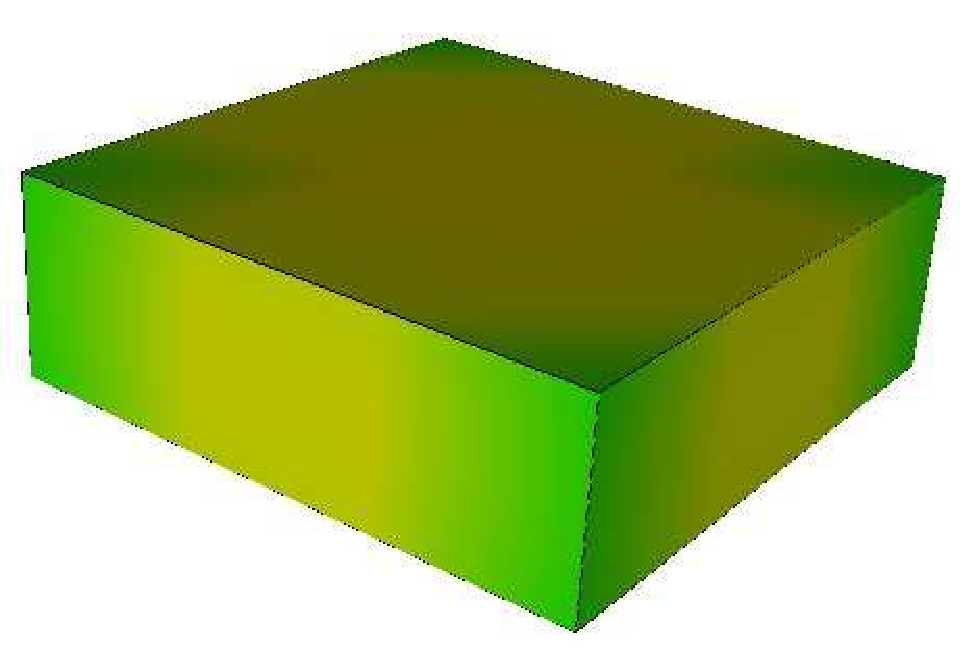
\includegraphics[width=\thumbnailwidth]{figures/Map} &
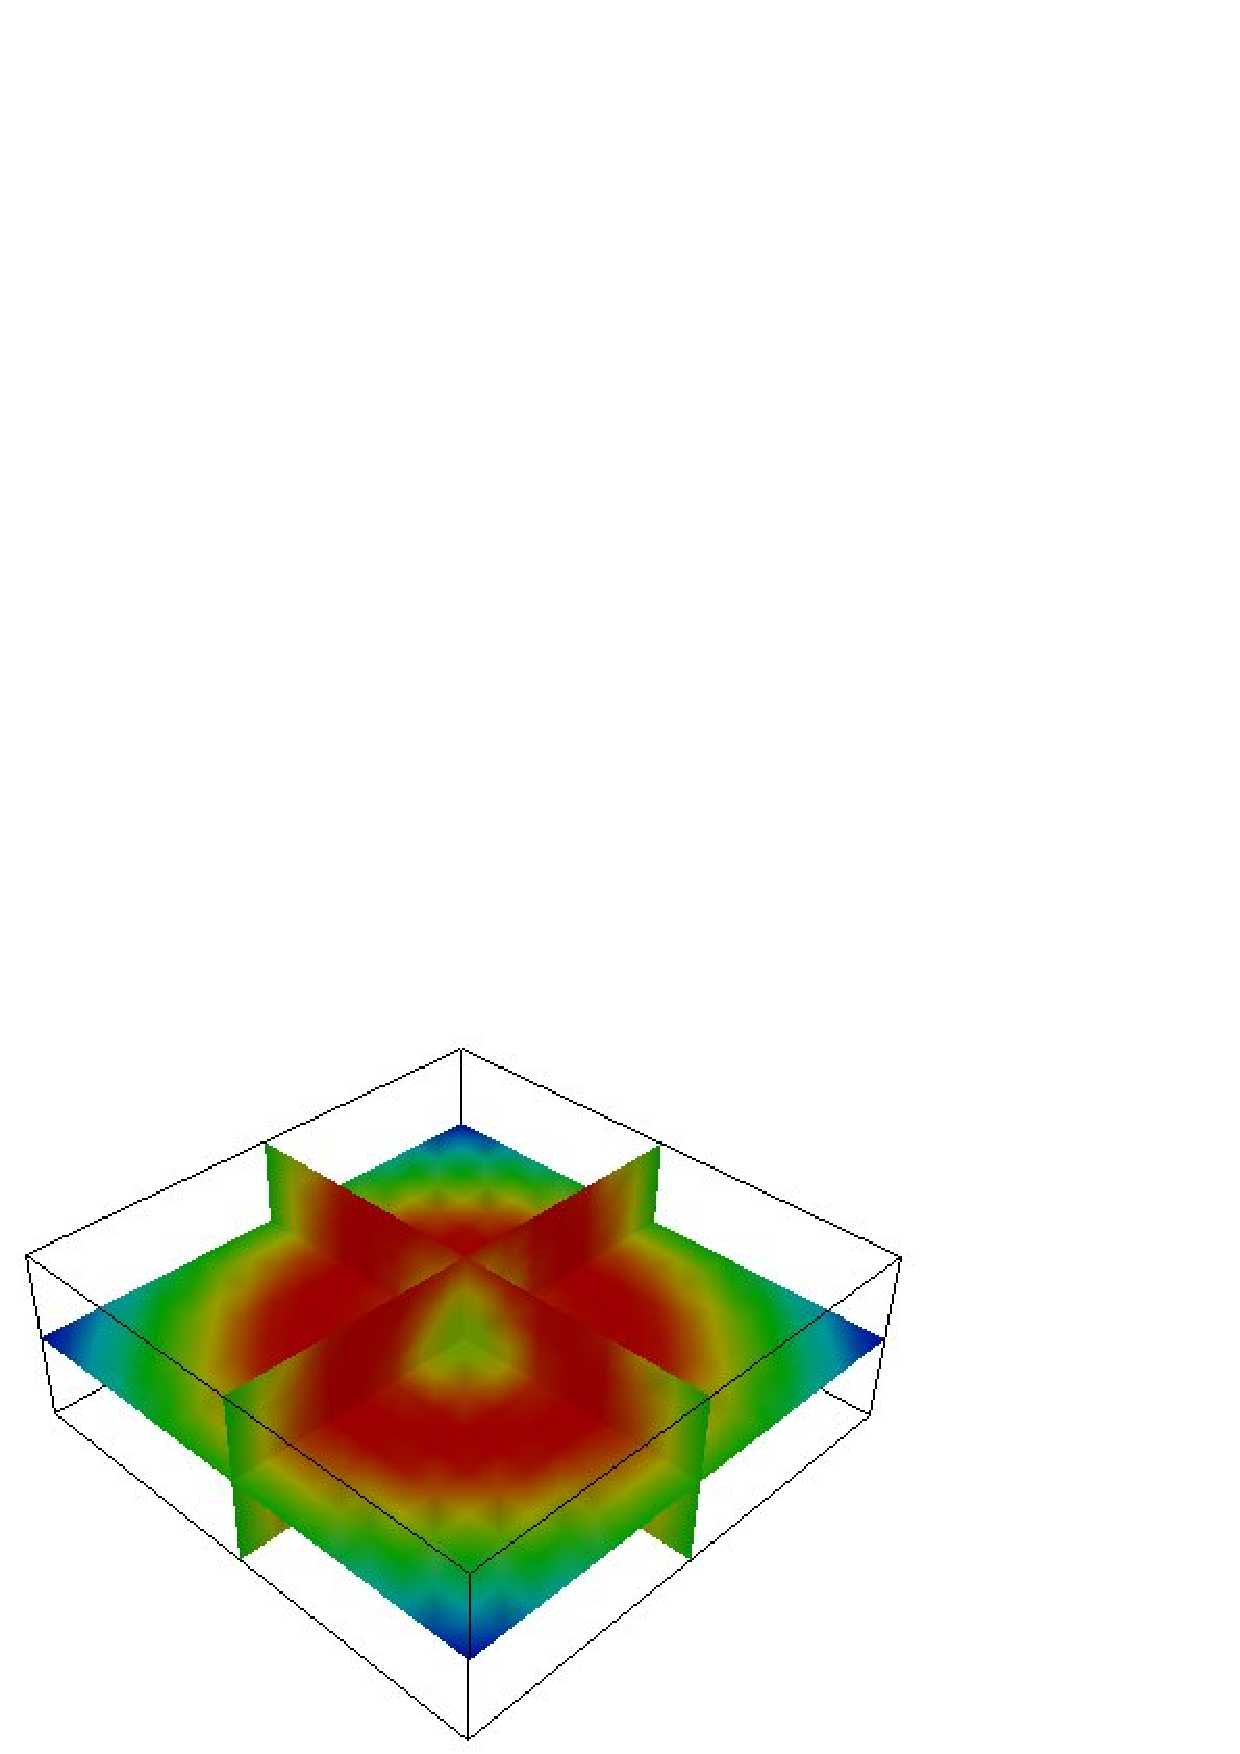
\includegraphics[width=\thumbnailwidth]{figures/MapOnPlaneCut} & 
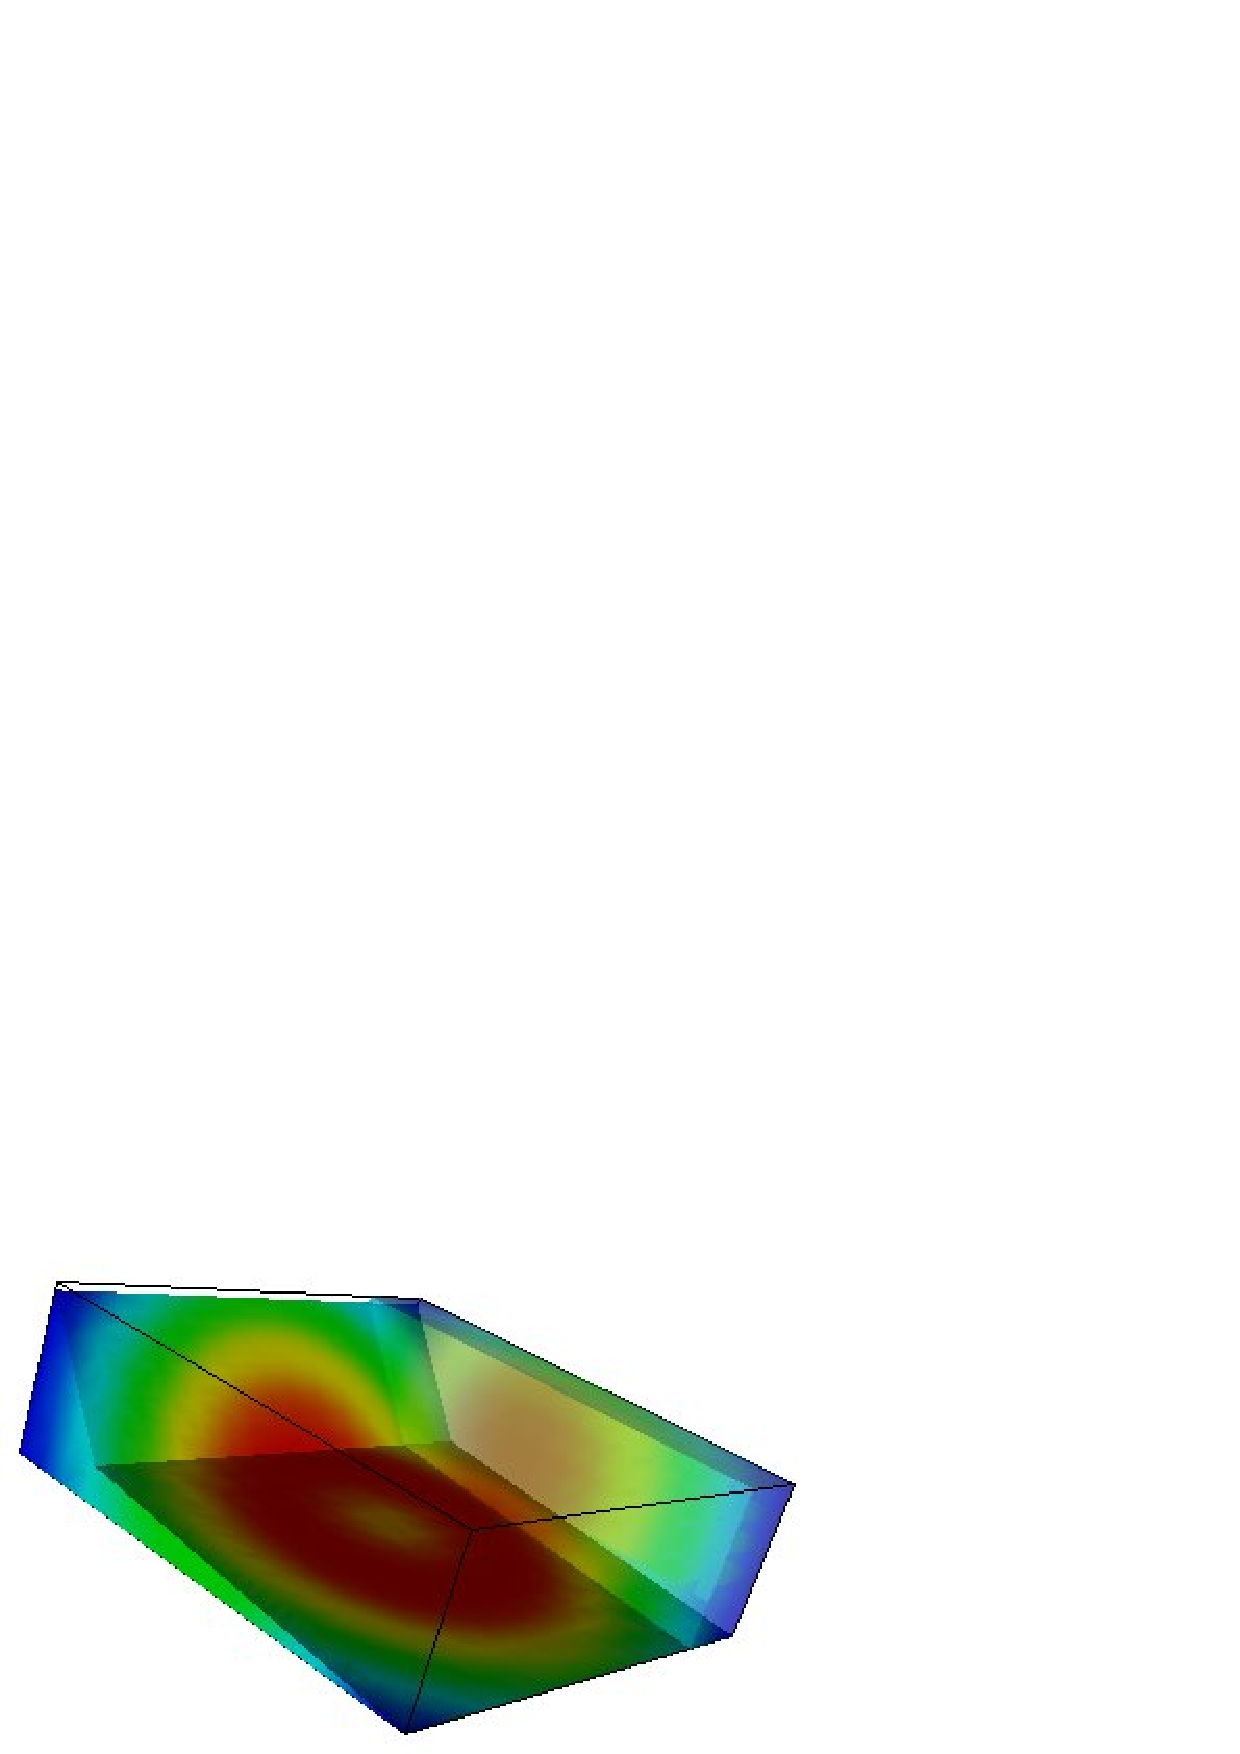
\includegraphics[width=\thumbnailwidth]{figures/MapOnPlaneClip} \\
Map & MapOnPlaneCut & MapOnPlaneClip \\
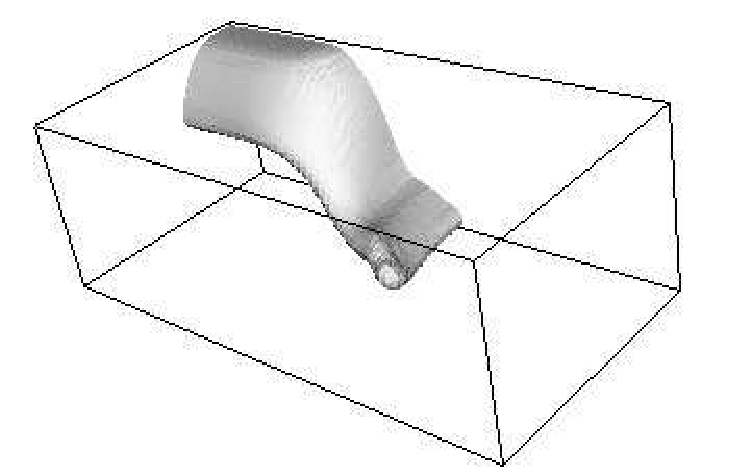
\includegraphics[width=\thumbnailwidth]{figures/MapOnScalarClip} &
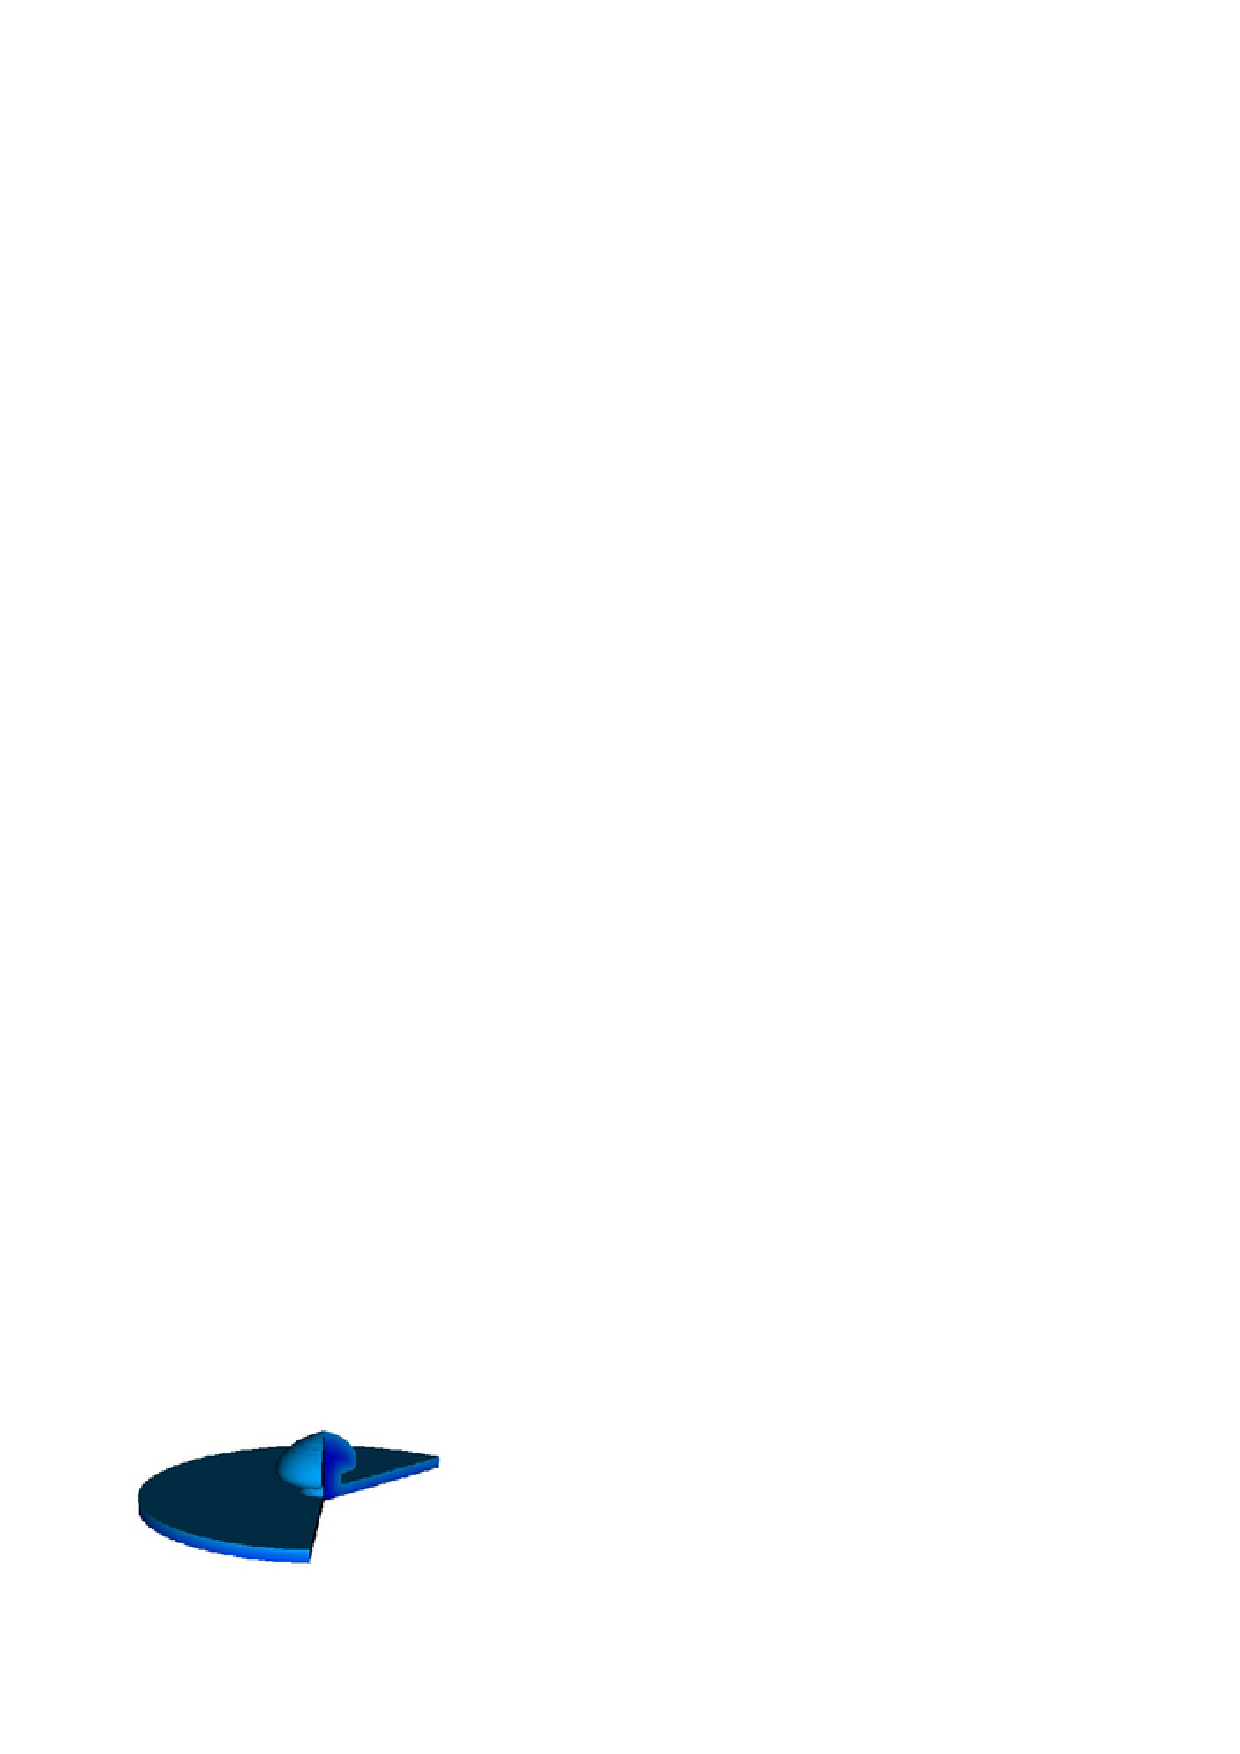
\includegraphics[width=\thumbnailwidth]{figures/MapOnScalarClipWithRotation} &
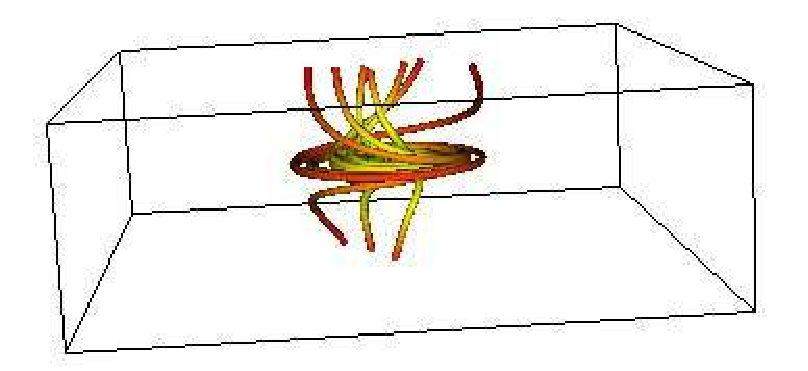
\includegraphics[width=\thumbnailwidth]{figures/StreamLine} \\
MapOnScalarClip & MapOnScalarClipWithRotation & Streamline \\ \\ \\
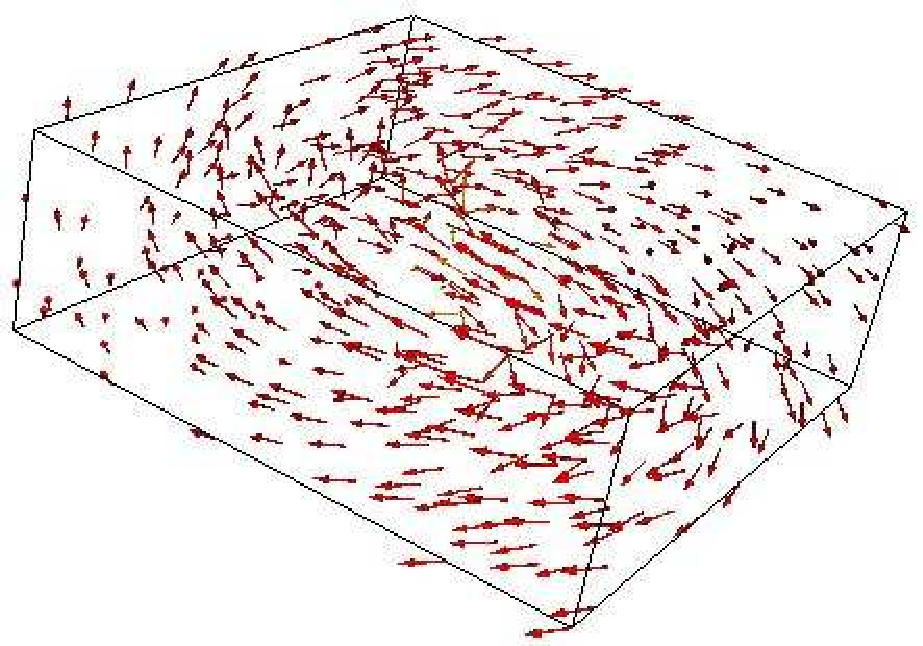
\includegraphics[width=\thumbnailwidth]{figures/Velocity} &
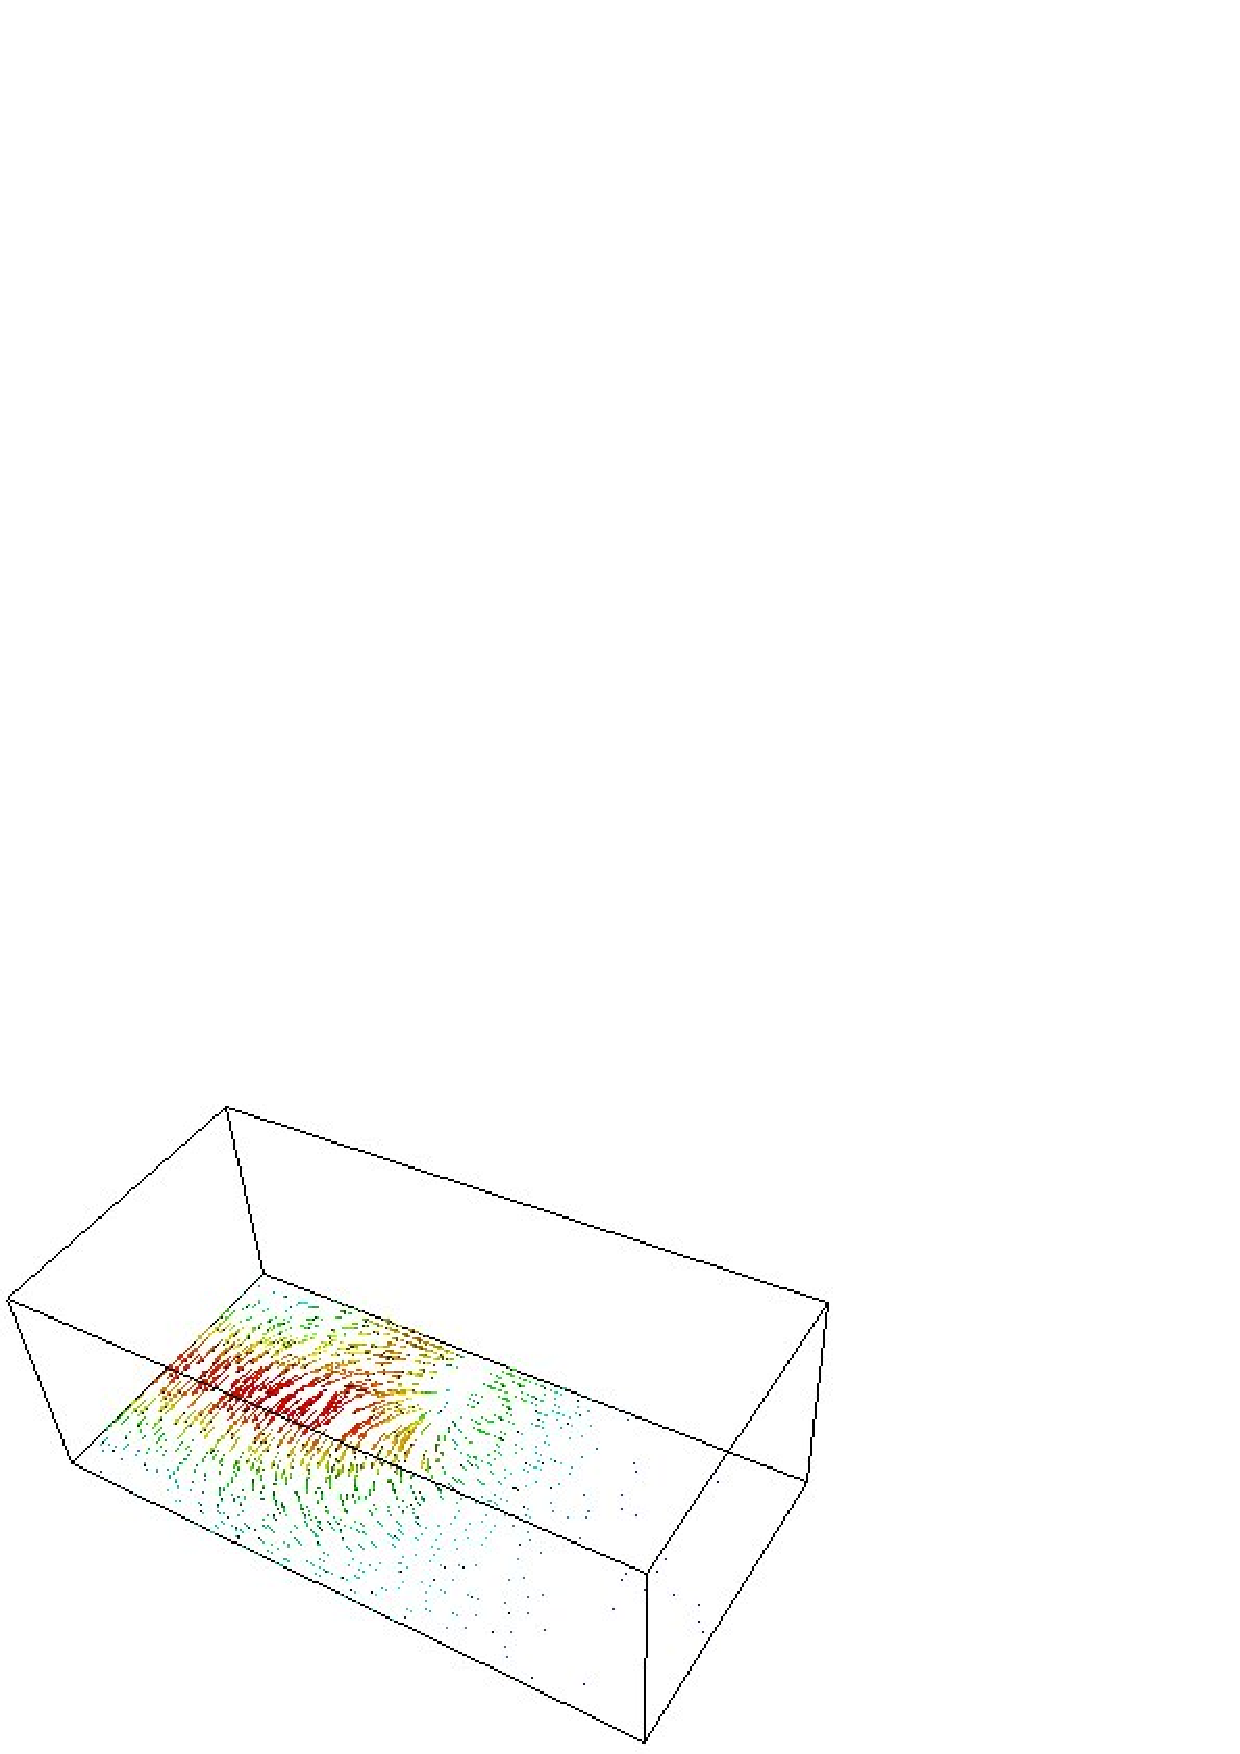
\includegraphics[width=\thumbnailwidth]{figures/VelocityOnPlaneCut} &
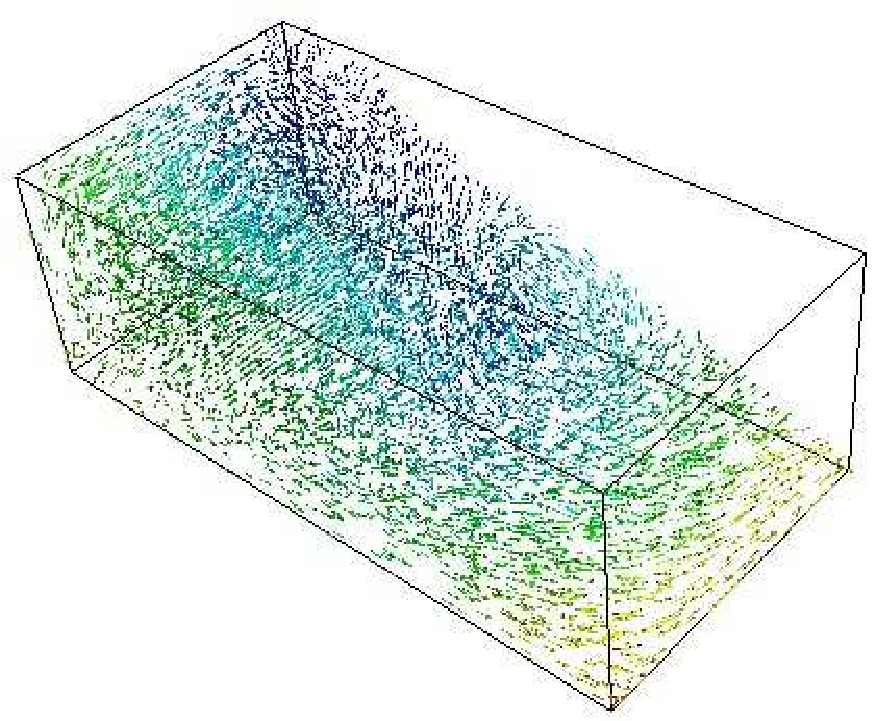
\includegraphics[width=\thumbnailwidth]{figures/VelocityOnPlaneClip} \\
Velocity & VelocityOnPlaneCut & VelocityOnPlaneClip \\ \\ \\
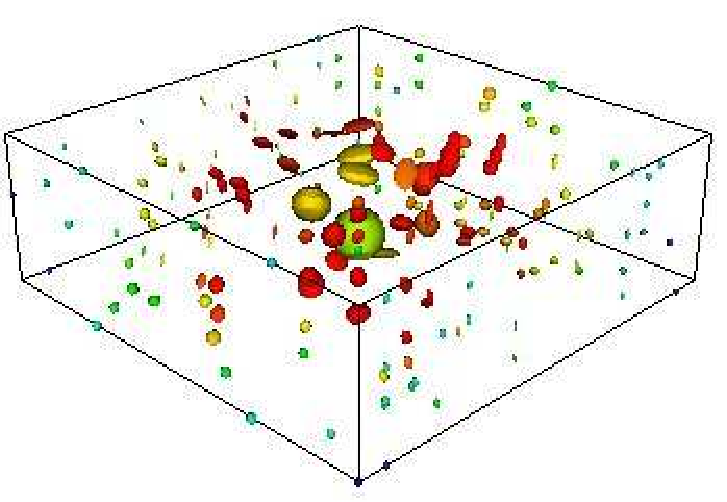
\includegraphics[width=\thumbnailwidth]{figures/Ellipsoid} &
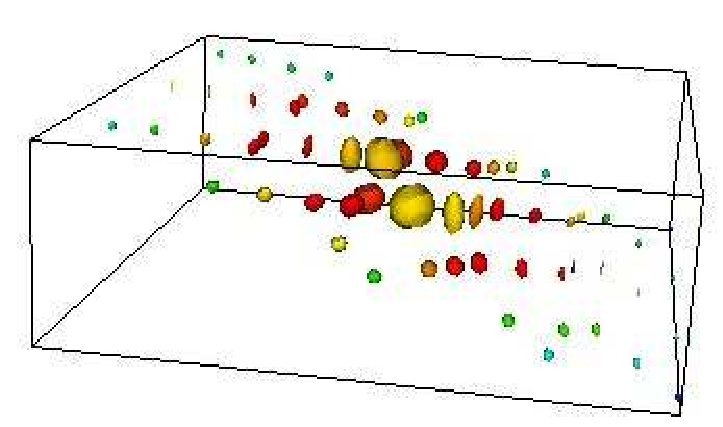
\includegraphics[width=\thumbnailwidth]{figures/EllipsoidOnPlaneCut} &
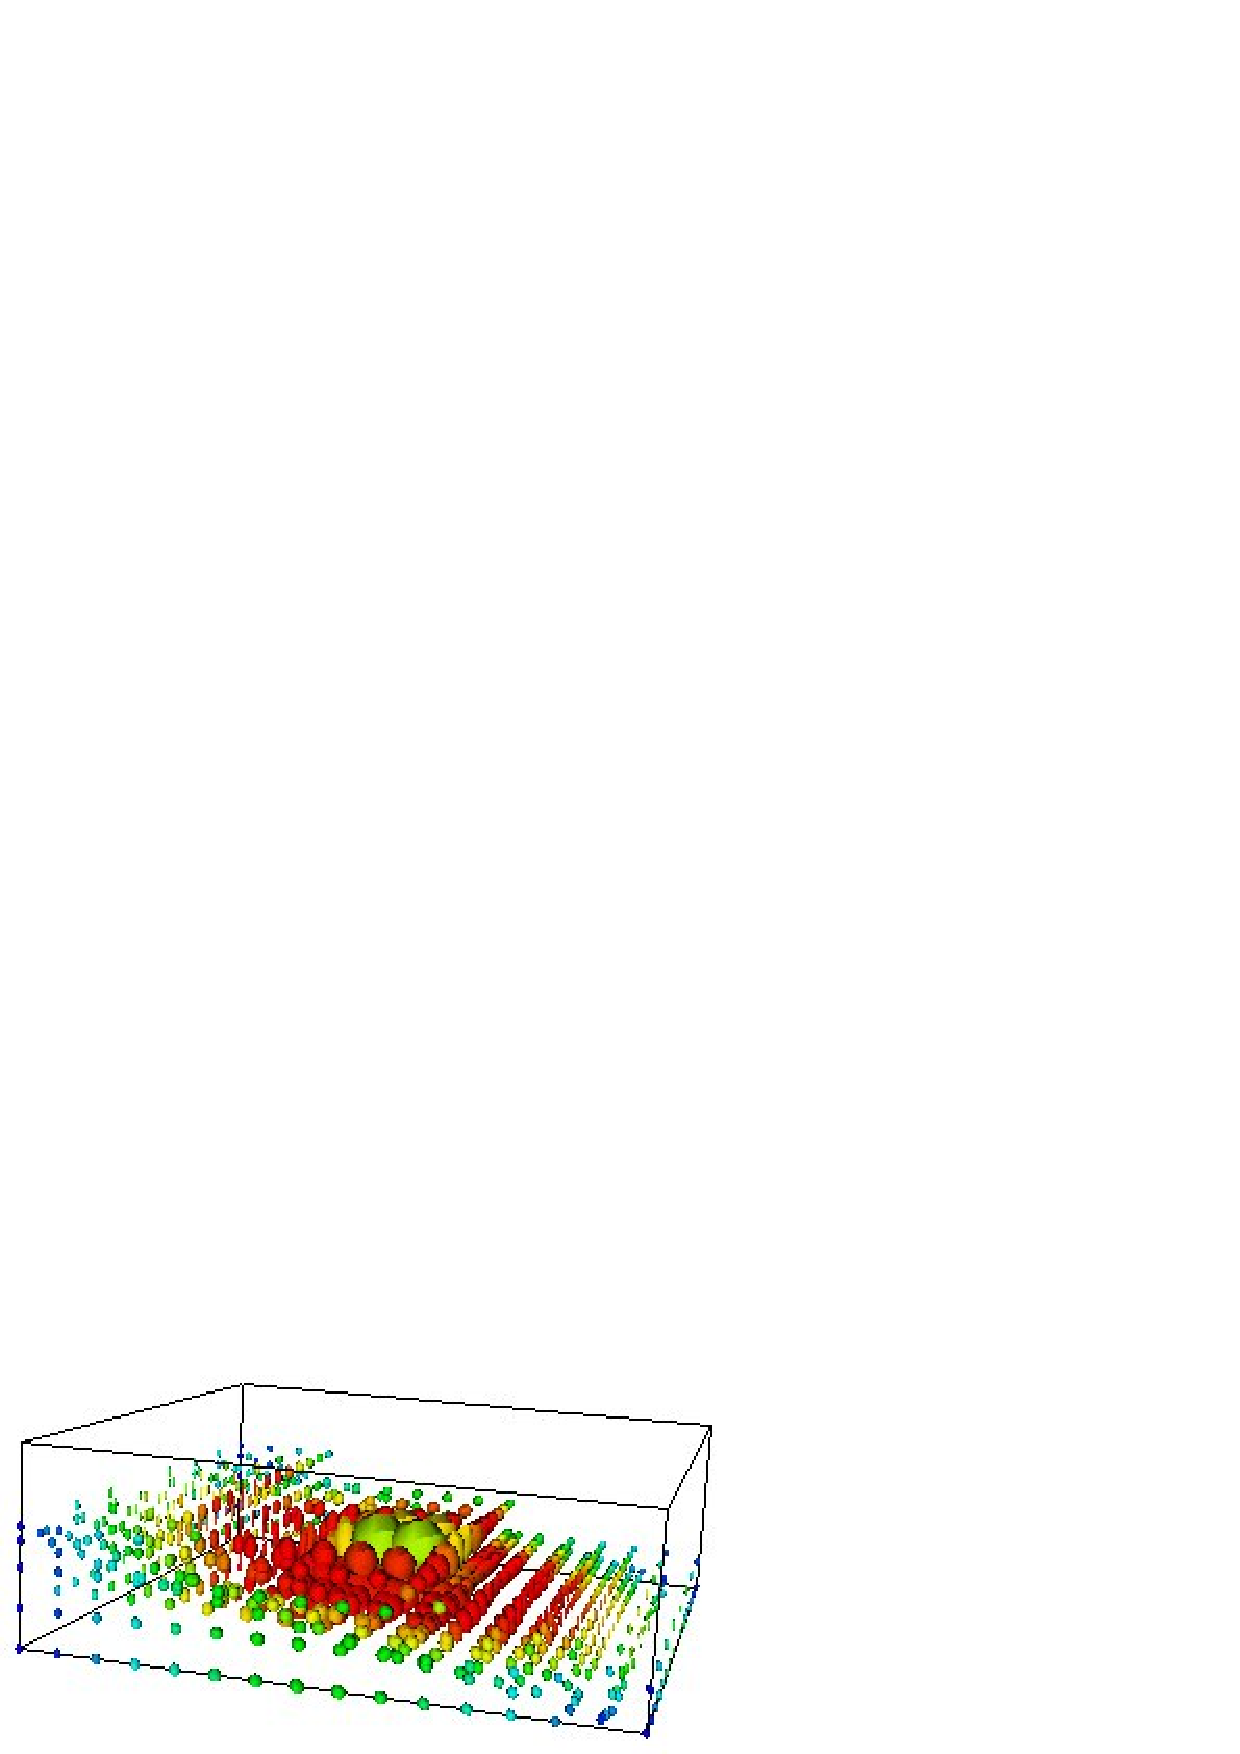
\includegraphics[width=\thumbnailwidth]{figures/EllipsoidOnPlaneClip} \\
Ellipsoid & EllipsoidOnPlaneCut & EllipsoidOnPlaneClip \\ \\
\end{tabular}
%\caption{Sample output}
\end{table}
%
\newpage
%
\begin{table}[t]
\begin{tabular}{c c c}
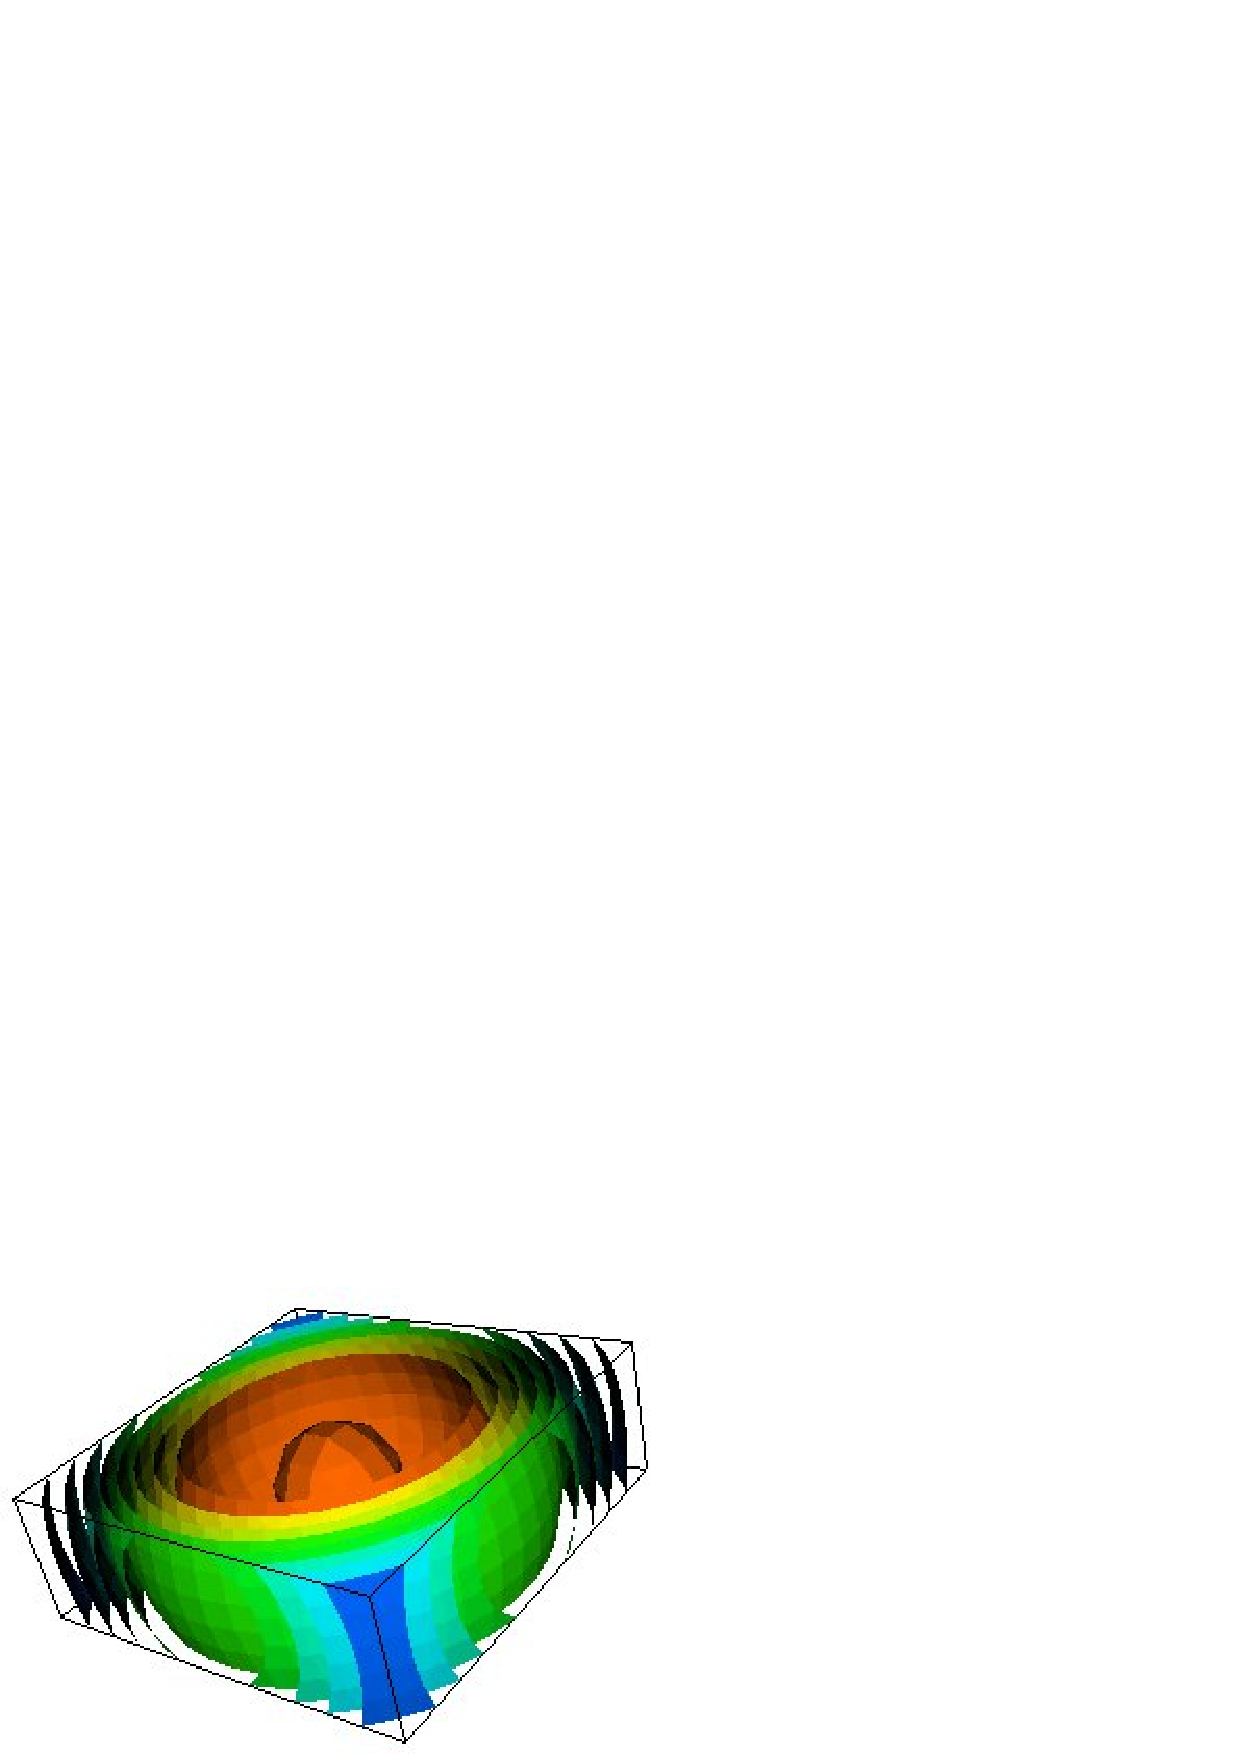
\includegraphics[width=\thumbnailwidth]{figures/Contour} &
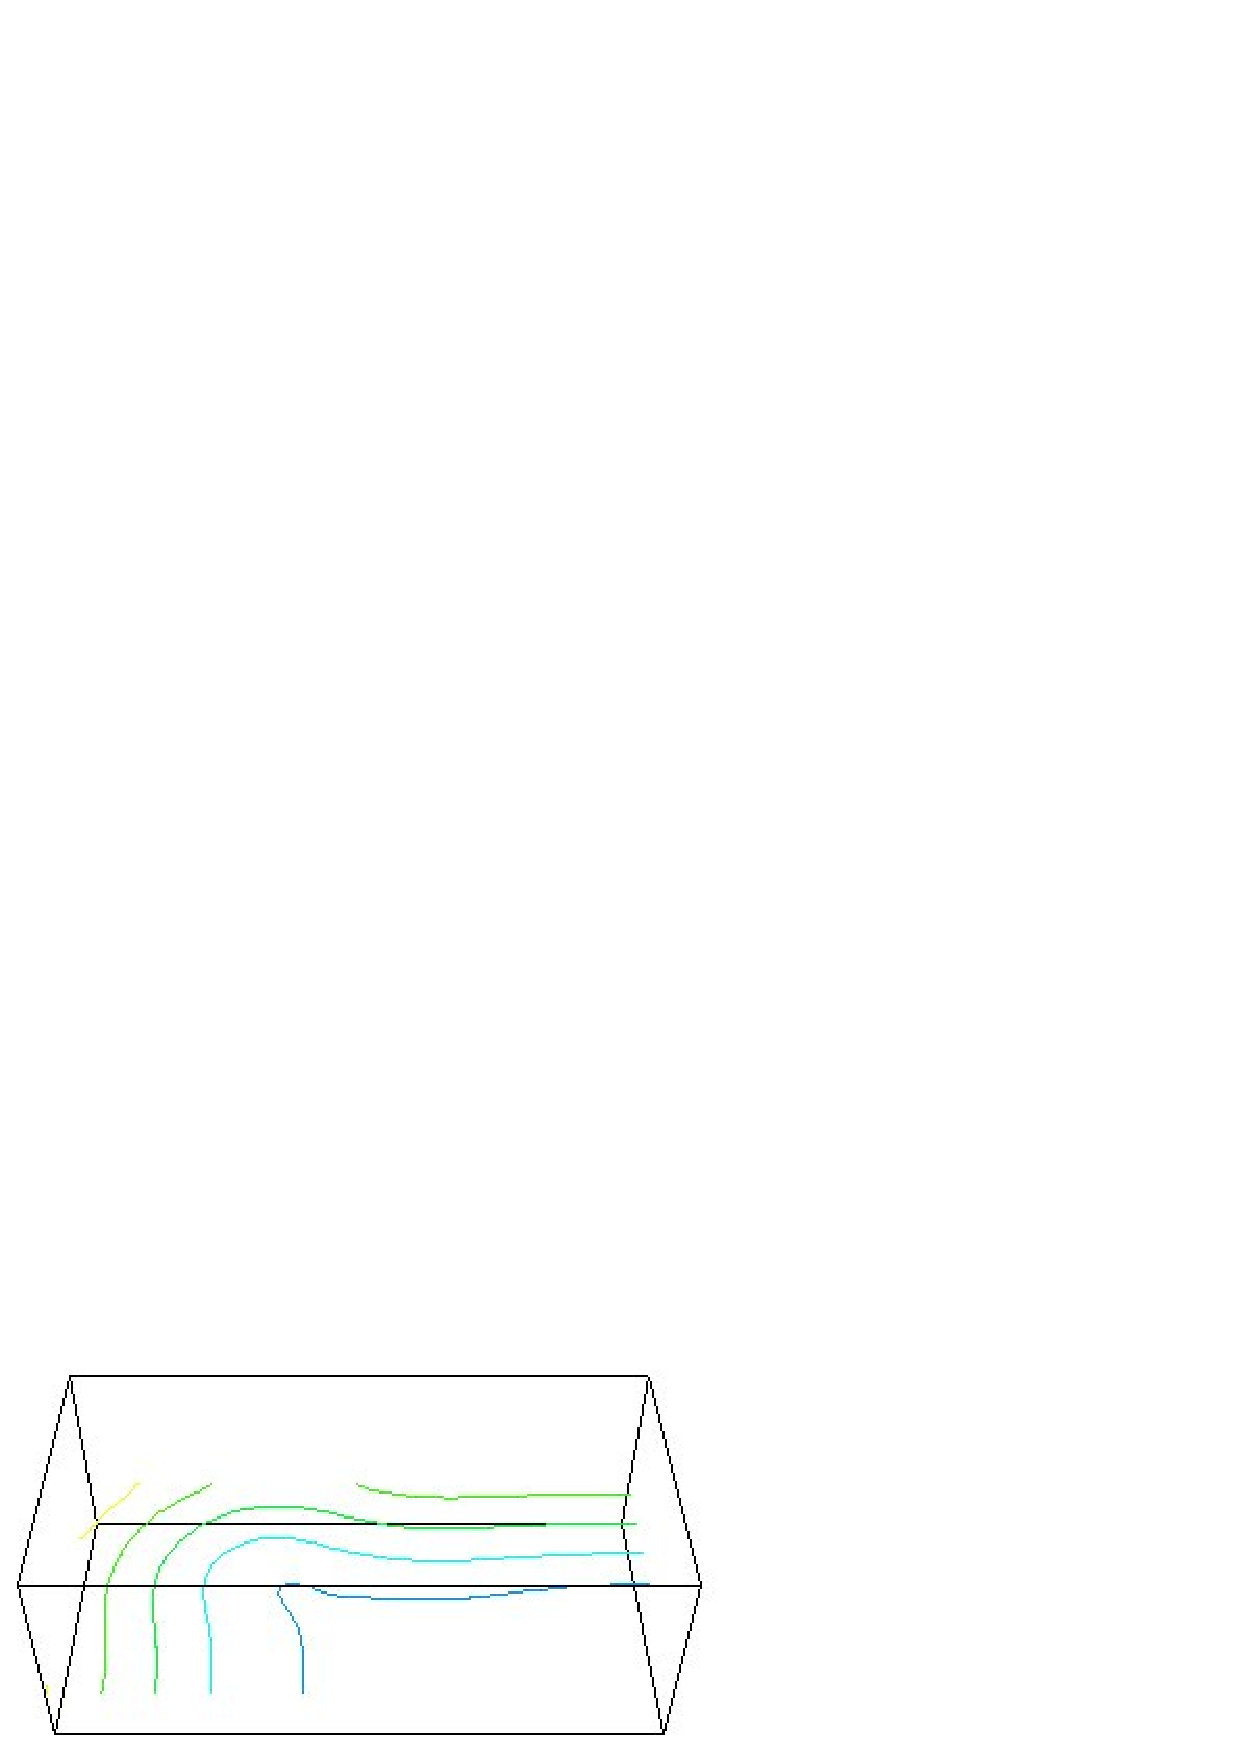
\includegraphics[width=\thumbnailwidth]{figures/ContourOnPlaneCut} &
\includegraphics[width=\thumbnailwidth]{figures/ContourOnPlaneClip} \\
Contour & ContourOnPlaneCut & ContourOnPlaneClip \\ \\ \\
\includegraphics[width=\thumbnailwidth]{figures/Carpet} &
\includegraphics[width=\thumbnailwidth]{figures/Rectangle} &
\includegraphics[width=\thumbnailwidth]{figures/Image} \\
Carpet & Rectangle & Image \\ \\ \\ \\ \\
\includegraphics[width=\thumbnailwidth]{figures/Text} &
\includegraphics[width=\thumbnailwidth]{figures/Logo} &
\includegraphics[width=\thumbnailwidth]{figures/Legend} \\
Text & Logo & Legend \\ \\
\end{tabular}
%\caption{Sample Output (continued)}
\end{table}





%%%%%%%%%%%%%%%%%%%%%%%%%%%%%%%%%%%%%%%%%%%%%%%%%%%%%%%%
%
% Copyright (c) 2003-2010 by University of Queensland
% Earth Systems Science Computational Center (ESSCC)
% http://www.uq.edu.au/esscc
%
% Primary Business: Queensland, Australia
% Licensed under the Open Software License version 3.0
% http://www.opensource.org/licenses/osl-3.0.php
%
%%%%%%%%%%%%%%%%%%%%%%%%%%%%%%%%%%%%%%%%%%%%%%%%%%%%%%%%

\chapter{The \finley Module}\label{CHAPTER ON FINLEY}
%\declaremodule{extension}{finley}
%\modulesynopsis{Solving linear, steady partial differential equations using finite elements}

{\it finley} is a library of C functions solving linear, steady partial
differential equations\index{partial differential equations} (PDEs) or systems
of PDEs using isoparametrical finite elements\index{FEM!isoparametrical}.
It supports unstructured 1D, 2D and 3D meshes.
The module \finley provides access to the library through the \LinearPDE class
of \escript supporting its full functionality.
{\it finley} is parallelized using the OpenMP\index{OpenMP} paradigm.

\section{Formulation}
For a single PDE that has a solution with a single component the linear PDE is
defined in the following form:
\begin{equation}\label{FINLEY.SINGLE.1}
\begin{array}{cl} &
\displaystyle{
\int_{\Omega}
A_{jl} \cdot v_{,j}u_{,l}+ B_{j} \cdot v_{,j} u+ C_{l} \cdot v u_{,l}+D \cdot vu \; d\Omega }  \\
+ & \displaystyle{\int_{\Gamma} d \cdot vu \; d{\Gamma} }
+  \displaystyle{\int_{\Gamma^{contact}} d^{contact} \cdot [v][u] \; d{\Gamma} } \\
= & \displaystyle{\int_{\Omega}  X_{j} \cdot v_{,j}+ Y \cdot v \; d\Omega }\\
+ & \displaystyle{\int_{\Gamma} y \cdot v \; d{\Gamma}}  +
\displaystyle{\int_{\Gamma^{contact}} y^{contact}\cdot [v] \; d{\Gamma}} \\
\end{array}
\end{equation}

\section{Meshes}
\label{FINLEY MESHES}

\begin{figure}
\centerline{\includegraphics{FinleyMesh}}
\caption{Subdivision of an Ellipse into triangles order 1 (\finleyelement{Tri3})}
\label{FINLEY FIG 0}
\end{figure}

To understand the usage of \finley one needs to have an understanding of how
the finite element meshes\index{FEM!mesh} are defined.
\fig{FINLEY FIG 0} shows an example of the subdivision of an ellipse into
so-called elements\index{FEM!elements}\index{element}.
In this case, triangles have been used but other forms of subdivisions can be
constructed, e.g. quadrilaterals or, in the three-dimensional case, into
tetrahedra and hexahedra. The idea of the finite element method is to
approximate the solution by a function which is a polynomial of a certain order
and is continuous across its boundary to neighbour elements.
In the example of \fig{FINLEY FIG 0} a linear polynomial is used on each
triangle. As one can see, the triangulation is quite a poor approximation of
the ellipse. It can be improved by introducing a midpoint on each element edge
then positioning those nodes located on an edge expected to describe the
boundary, onto the boundary.
In this case the triangle gets a curved edge which requires a parameterization
of the triangle using a quadratic polynomial.
For this case, the solution is also approximated by a piecewise quadratic
polynomial (which explains the name isoparametrical elements),
see \Ref{Zienc,NumHand} for more details.
\finley also supports macro elements\index{macro elements}.
For these elements a piecewise linear approximation is used on an element which
is further subdivided (in the case of \finley halved).
As such, these elements do not provide more than a further mesh refinement but
should be used in the case of incompressible flows, see \class{StokesProblemCartesian}.
For these problems a linear approximation of the pressure across the element is
used (use the \ReducedSolutionFS) while the refined element is used to
approximate velocity. So a macro element provides a continuous pressure
approximation together with a velocity approximation on a refined mesh.
This approach is necessary to make sure that the incompressible flow has a
unique solution.

The union of all elements defines the domain of the PDE.
Each element is defined by the nodes used to describe its shape.
In \fig{FINLEY FIG 0} the element, which has type \finleyelement{Tri3}, with
element reference number $19$\index{element!reference number} is defined by the
nodes with reference numbers $9$, $11$ and $0$\index{node!reference number}.
Notice that the order is counterclockwise.
The coefficients of the PDE are evaluated at integration nodes with each
individual element.
For quadrilateral elements a Gauss quadrature scheme is used.
In the case of triangular elements a modified form is applied.
The boundary of the domain is also subdivided into elements\index{element!face}.
In \fig{FINLEY FIG 0} line elements with two nodes are used.
The elements are also defined by their describing nodes, e.g. the face element
with reference number $20$, which has type \finleyelement{Line2}, is defined by
the nodes with the reference numbers $11$ and $0$.
Again the order is crucial, if moving from the first to second node the domain
has to lie on the left hand side (in the case of a two-dimensional surface
element the domain has to lie on the left hand side when moving
counterclockwise). If the gradient on the surface of the domain is to be
calculated rich face elements need to be used. Rich elements on a face are
identical to interior elements but with a modified order of nodes such that the
'first' face of the element aligns with the surface of the domain.
In \fig{FINLEY FIG 0} elements of the type \finleyelement{Tri3Face} are used.
The face element reference number $20$ as a rich face element is defined by the
nodes with reference numbers $11$, $0$ and $9$.
Notice that the face element $20$ is identical to the interior element $19$
except that, in this case, the order of the node is different to align the first
edge of the triangle (which is the edge starting with the first node) with the
boundary of the domain.

Be aware that face elements and elements in the interior of the domain must
match, i.e. a face element must be the face of an interior element or, in case
of a rich face element, it must be identical to an interior element.
If no face elements are specified \finley implicitly assumes homogeneous
natural boundary conditions\index{natural boundary conditions!homogeneous},
i.e. \var{d}=$0$ and \var{y}=$0$, on the entire boundary of the domain.
For inhomogeneous natural boundary conditions\index{natural boundary conditions!inhomogeneous},
the boundary must be described by face elements.

\begin{figure}
\centerline{\includegraphics{FinleyContact}}
\caption{Mesh around a contact region (\finleyelement{Rec4})}
\label{FINLEY FIG 01}
\end{figure}

If discontinuities of the PDE solution are considered, contact
elements\index{element!contact}\index{contact conditions} are introduced to
describe the contact region $\Gamma^{contact}$ even if $d^{contact}$ and
$y^{contact}$ are zero.
\fig{FINLEY FIG 01} shows a simple example of a mesh of rectangular elements
around a contact region $\Gamma^{contact}$\index{element!contact}.
The contact region is described by the elements $4$, $3$ and $6$.
Their element type is \finleyelement{Line2_Contact}.
The nodes $9$, $12$, $6$ and $5$ define contact element $4$, where the
coordinates of nodes $12$ and $5$ and nodes $4$ and $6$ are identical, with the
idea that nodes $12$ and $9$ are located above and nodes $5$ and $6$ below the
contact region.
Again, the order of the nodes within an element is crucial.
There is also the option of using rich elements if the gradient is to be
calculated on the contact region. Similarly to the rich face elements these
are constructed from two interior elements by reordering the nodes such that
the 'first' face of the element above and the 'first' face of the element below
the contact regions line up. The rich version of element $4$ is of type
\finleyelement{Rec4Face_Contact} and is defined by the nodes $9$, $12$, $16$,
$18$, $6$, $5$, $0$ and $2$.
\tab{FINLEY TAB 1} shows the interior element types and the corresponding
element types to be used on the face and contacts.
\fig{FINLEY.FIG:1}, \fig{FINLEY.FIG:2} and \fig{FINLEY.FIG:4} show the ordering
of the nodes within an element.

\begin{table}
\centering
\begin{tabular}{l|llll}
\textbf{interior}&\textbf{face}&\textbf{rich face}&\textbf{contact}&\textbf{rich contact}\\
\hline
\finleyelement{Line2} & \finleyelement{Point1} & \finleyelement{Line2Face} & \finleyelement{Point1_Contact} & \finleyelement{Line2Face_Contact}\\
\finleyelement{Line3} & \finleyelement{Point1} & \finleyelement{Line3Face} & \finleyelement{Point1_Contact} & \finleyelement{Line3Face_Contact}\\
\finleyelement{Tri3} & \finleyelement{Line2} & \finleyelement{Tri3Face} & \finleyelement{Line2_Contact} & \finleyelement{Tri3Face_Contact}\\
\finleyelement{Tri6} & \finleyelement{Line3} & \finleyelement{Tri6Face} & \finleyelement{Line3_Contact} & \finleyelement{Tri6Face_Contact}\\
\finleyelement{Rec4} & \finleyelement{Line2} & \finleyelement{Rec4Face} & \finleyelement{Line2_Contact} & \finleyelement{Rec4Face_Contact}\\
\finleyelement{Rec8} & \finleyelement{Line3} & \finleyelement{Rec8Face} & \finleyelement{Line3_Contact} & \finleyelement{Rec8Face_Contact}\\
\finleyelement{Rec9} & \finleyelement{Line3} & \finleyelement{Rec9Face} & \finleyelement{Line3_Contact} & \finleyelement{Rec9Face_Contact}\\
\finleyelement{Tet4} & \finleyelement{Tri6} & \finleyelement{Tet4Face} & \finleyelement{Tri6_Contact} & \finleyelement{Tet4Face_Contact}\\
\finleyelement{Tet10} & \finleyelement{Tri9} & \finleyelement{Tet10Face} & \finleyelement{Tri9_Contact} & \finleyelement{Tet10Face_Contact}\\
\finleyelement{Hex8} & \finleyelement{Rec4} & \finleyelement{Hex8Face} & \finleyelement{Rec4_Contact} & \finleyelement{Hex8Face_Contact}\\
\finleyelement{Hex20} & \finleyelement{Rec8} & \finleyelement{Hex20Face} & \finleyelement{Rec8_Contact} & \finleyelement{Hex20Face_Contact}\\
\finleyelement{Hex27} & \finleyelement{Rec9} & N/A & N/A & N/A\\
\finleyelement{Hex27Macro} & \finleyelement{Rec9Macro} & N/A & N/A & N/A\\
\finleyelement{Tet10Macro} & \finleyelement{Tri6Macro} & N/A & N/A & N/A\\
\finleyelement{Rec9Macro} & \finleyelement{Line3Macro} & N/A & N/A & N/A\\
\finleyelement{Tri6Macro} & \finleyelement{Line3Macro} & N/A & N/A & N/A\\
\end{tabular}
\caption{Finley elements and corresponding elements to be used on domain faces
and contacts.
The rich types have to be used if the gradient of the function is to be
calculated on faces and contacts, respectively.}
\label{FINLEY TAB 1}
\end{table}

The native \finley file format is defined as follows.
Each node \var{i} has \var{dim} spatial coordinates \var{Node[i]}, a reference
number \var{Node_ref[i]}, a degree of freedom \var{Node_DOF[i]} and a tag
\var{Node_tag[i]}.
In most cases \var{Node_DOF[i]}=\var{Node_ref[i]} however, for periodic
boundary conditions, \var{Node_DOF[i]} is chosen differently, see example below.
The tag can be used to mark nodes sharing the same properties.
Element \var{i} is defined by the \var{Element_numNodes} nodes
\var{Element_Nodes[i]} which is a list of node reference numbers.
The order of these is crucial. Each element has a reference number
\var{Element_ref[i]} and a tag \var{Element_tag[i]}.
The tag can be used to mark elements sharing the same properties.
For instance elements above a contact region are marked with tag $2$ and
elements below a contact region are marked with tag $1$.
\var{Element_Type} and \var{Element_Num} give the element type and the number
of elements in the mesh.
Analogue notations are used for face and contact elements.
The following \PYTHON script prints the mesh definition in the \finley file
format:
\begin{python}
  print("%s\n"%mesh_name)
  # node coordinates:
  print("%dD-nodes %d\n"%(dim, numNodes))
  for i in range(numNodes):
     print("%d %d %d"%(Node_ref[i], Node_DOF[i], Node_tag[i]))
     for j in range(dim): print(" %e"%Node[i][j])
     print("\n")
  # interior elements
  print("%s %d\n"%(Element_Type, Element_Num))
  for i in range(Element_Num):
     print("%d %d"%(Element_ref[i], Element_tag[i]))
     for j in range(Element_numNodes): print(" %d"%Element_Nodes[i][j])
     print("\n")
  # face elements
  print("%s %d\n"%(FaceElement_Type, FaceElement_Num))
  for i in range(FaceElement_Num):
     print("%d %d"%(FaceElement_ref[i], FaceElement_tag[i]))
     for j in range(FaceElement_numNodes): print(" %d"%FaceElement_Nodes[i][j])
     print("\n")
  # contact elements
  print("%s %d\n"%(ContactElement_Type, ContactElement_Num))
  for i in range(ContactElement_Num):
     print("%d %d"%(ContactElement_ref[i], ContactElement_tag[i]))
     for j in range(ContactElement_numNodes): print(" %d"%ContactElement_Nodes[i][j])
     print("\n")
  # point sources (not supported yet)
  print("Point1 0")
\end{python}

The following example of a mesh file defines the mesh shown in \fig{FINLEY FIG 01}:
\begin{verbatim}
Example 1
2D Nodes 16
0   0 0 0.   0.
2   2 0 0.33 0.
3   3 0 0.66 0.
7   4 0 1.   0.
5   5 0 0.   0.5
6   6 0 0.33 0.5
8   8 0 0.66 0.5
10 10 0 1.0  0.5
12 12 0 0.   0.5
9   9 0 0.33 0.5
13 13 0 0.66 0.5
15 15 0 1.0  0.5
16 16 0 0.   1.0
18 18 0 0.33 1.0
19 19 0 0.66 1.0
20 20 0 1.0  1.0
Rec4 6
 0 1  0  2  6  5
 1 1  2  3  8  6
 2 1  3  7 10  8
 5 2 12  9 18 16
 7 2 13 19 18  9
10 2 20 19 13 15
Line2 0
Line2_Contact 3
 4 0  9 12  6 5
 3 0 13  9  8 6
 6 0 15 13 10 8
Point1 0
\end{verbatim}
Notice that the order in which the nodes and elements are given is arbitrary.
In the case that rich contact elements are used the contact element section
gets the form
\begin{verbatim}
Rec4Face_Contact 3
 4 0  9 12 16 18  6  5  0  2
 3 0 13  9 18 19  8  6  2  3
 6 0 15 13 19 20 10  8  3  7
\end{verbatim}
Periodic boundary conditions\index{boundary conditions!periodic} can be
introduced by altering \var{Node_DOF}.
It allows identification of nodes even if they have different physical locations.
For instance, to enforce periodic boundary conditions at the face $x_0=0$ and
$x_0=1$ one identifies the degrees of freedom for nodes $0$, $5$, $12$ and $16$
with the degrees of freedom for $7$, $10$, $15$ and $20$, respectively.
The node section of the \finley mesh now reads:
\begin{verbatim}
2D Nodes 16
0   0 0 0.   0.
2   2 0 0.33 0.
3   3 0 0.66 0.
7   0 0 1.   0.
5   5 0 0.   0.5
6   6 0 0.33 0.5
8   8 0 0.66 0.5
10  5 0 1.0  0.5
12 12 0 0.   0.5
9   9 0 0.33 0.5
13 13 0 0.66 0.5
15 12 0 1.0  0.5
16 16 0 0.   1.0
18 18 0 0.33 1.0
19 19 0 0.66 1.0
20 16 0 1.0  1.0
\end{verbatim}

\clearpage

%%%%%%%%%%%%%%%%%%%%%%%%%%%%%%%%%%%%%%%%%%%%%%%%%%%%%%%%%%%%%%%%%%%%%%%%%%%%%%
% Copyright (c) 2003-2015 by University of Queensland
% http://www.uq.edu.au
%
% Primary Business: Queensland, Australia
% Licensed under the Open Software License version 3.0
% http://www.opensource.org/licenses/osl-3.0.php
%
% Development until 2012 by Earth Systems Science Computational Center (ESSCC)
% Development 2012-2013 by School of Earth Sciences
% Development from 2014 by Centre for Geoscience Computing (GeoComp)
%
%%%%%%%%%%%%%%%%%%%%%%%%%%%%%%%%%%%%%%%%%%%%%%%%%%%%%%%%%%%%%%%%%%%%%%%%%%%%%%

\setlength{\unitlength}{1mm}

\newsavebox{\HLa}
\savebox{\HLa}(0,0)
  {\put(0,0){\circle*{2}}
   \thicklines \put(1,0){\line(1,0){28}}
   \put(30,0){\circle*{2}} }

\newsavebox{\HLathin}
\savebox{\HLathin}(0,0)
  {\put(0,0){\circle{2}}
   \thinlines \put(1,0){\line(1,0){28}}
   \put(30,0){\circle{2}} }

\newsavebox{\VLa}
\savebox{\VLa}(0,30)
  {\put(0,0){\circle*{2}}
   \thicklines \put(0,1){\line(0,1){28}}
   \put(0,30){\circle*{2}} }

\newsavebox{\VLathin}
\savebox{\VLathin}(0,30)
  {\put(0,0){\circle{2}}
   \thinlines \put(0,1){\line(0,1){28}}
   \put(0,30){\circle{2}} }

\newsavebox{\SLax}
\savebox{\SLax}(0,30)
  {\thicklines \put(0,0){\line(-1,1){30}}
   \put(0,0){\circle*{2}}
   \put(-30,30){\circle*{2}} }

\newsavebox{\SLaa}
\savebox{\SLaa}(0,15)
  {\thicklines \put(0,0){\line(-4,3){20}}
   \put(0,0){\circle*{2}}
   \put(-20,15){\circle*{2}} }

\newsavebox{\SLab}
\savebox{\SLab}(0,-15)
  {\thicklines \put(0,0){\line(-4,-3){20}}
   \put(0,0){\circle*{2}}
   \put(-20,-15){\circle*{2}} }

\newsavebox{\SLabthin}
\savebox{\SLabthin}(0,-15)
  {\thinlines \put(-0.7,-0.7){\line(-4,-3){18.7}}
   \put(0,0){\circle{2}}
   \put(-20,-15){\circle{2}} }

\newsavebox{\SLac}
\savebox{\SLac}(0,15)
  {\thicklines \put(0,0){\line(-2,3){10}}
   \put(0,0){\circle*{2}}
   \put(-10,15){\circle*{2}} }

\newsavebox{\SLacthin}
\savebox{\SLacthin}(0,15)
  {\thinlines \put(0,0){\line(-2,3){9.4}}
   \put(0,0){\circle{2}}
   \put(-10,15){\circle{2}} }


\newsavebox{\HLd}
\savebox{\HLd}(0,0)
  {\put(0,0){\circle*{2}}
   \put(10,0){\circle*{2}}
   \thicklines \put(1,0){\line(1,0){28}}
   \put(20,0){\circle*{2}}
   \put(30,0){\circle*{2}} }

\newsavebox{\HLdthin}
\savebox{\HLdthin}(0,0)
  {\put(0,0){\circle{2}}
   \put(10,0){\circle{2}}
   \thinlines \multiput(1,0)(10,0){3}{\line(1,0){8}}
   \put(20,0){\circle{2}}
   \put(30,0){\circle{2}} }

\newsavebox{\VLd}
\savebox{\VLd}(0,30)
  {\put(0,0){\circle*{2}}
   \put(0,10){\circle*{2}}
   \thicklines \put(0,1){\line(0,1){28}}
   \put(0,20){\circle*{2}}
   \put(0,30){\circle*{2}} }

\newsavebox{\VLdthin}
\savebox{\VLdthin}(0,30)
  {\put(0,0){\circle{2}}
   \put(0,10){\circle{2}}
   \thinlines \multiput(0,1)(0,10){3}{\line(0,1){8}}
   \put(0,20){\circle{2}}
   \put(0,30){\circle{2}} }

\newsavebox{\SLf}
\savebox{\SLf}(0,30)
  {\thicklines \put(0,0){\line(-1,1){30}}
   \put(0,0){\circle*{2}}
   \put(-10,10){\circle*{2}}
   \put(-20,20){\circle*{2}}
   \put(-30,30){\circle*{2}} }

\newsavebox{\SLad}
\savebox{\SLad}(0,15)
  {\thicklines \put(0,0){\line(-4,3){20}}
   \put(0,0){\circle*{2}}
   \put(-6.66,5){\circle*{2}}
   \put(-13.33,10){\circle*{2}}
   \put(-20,15){\circle*{2}} }

\newsavebox{\SLbd}
\savebox{\SLbd}(0,-15)
  {\thicklines \put(0,0){\line(-4,-3){20}}
   \put(0,0){\circle*{2}}
   \put(-6.66,-5){\circle*{2}}
   \put(-13.33,-10){\circle*{2}}
   \put(-20,-15){\circle*{2}} }

\newsavebox{\SLbdthin}
\savebox{\SLbdthin}(0,-15)
  {\thinlines \multiput(-0.7,-0.7)(-6.66,-5){3}{\line(-4,-3){5.1}}
   \put(0,0){\circle{2}}
   \put(-6.66,-5){\circle{2}}
   \put(-13.33,-10){\circle{2}}
   \put(-20,-15){\circle{2}} }

\newsavebox{\SLcd}
\savebox{\SLcd}(0,15)
  {\thicklines \put(0,0){\line(-2,3){10}}
   \put(0,0){\circle*{2}}
   \put(-3.33,5){\circle*{2}}
   \put(-6.66,10){\circle*{2}}
   \put(-10,15){\circle*{2}} }

\newsavebox{\SLcdthin}
\savebox{\SLcdthin}(0,15)
  {\thinlines \multiput(-0.6,0.8)(-3.33,5){3}{\line(-2,3){2.35}}
   \put(0,0){\circle{2}}
   \put(-3.33,5){\circle{2}}
   \put(-6.66,10){\circle{2}}
   \put(-10,15){\circle{2}} }

\newsavebox{\HLe}
\savebox{\HLe}(0,0)
  {\put(0,0){\circle*{2}}
   \put(15,0){\circle*{2}}
   \thicklines \put(1,0){\line(1,0){28}}
   \put(30,0){\circle*{2}} }

\newsavebox{\HLethin}
\savebox{\HLethin}(0,0)
  {\put(0,0){\circle{2}}
   \put(15,0){\circle{2}}
   \thinlines \multiput(1,0)(15,0){2}{\line(1,0){13}}
   \put(30,0){\circle{2}} }

\newsavebox{\VLe}
\savebox{\VLe}(0,30)
  {\put(0,0){\circle*{2}}
   \put(0,15){\circle*{2}}
   \thicklines \put(0,1){\line(0,1){28}}
   \put(0,30){\circle*{2}} }

\newsavebox{\VLethin}
\savebox{\VLethin}(0,30)
  {\put(0,0){\circle{2}}
   \put(0,15){\circle{2}}
   \thinlines \multiput(0,1)(0,15){2}{\line(0,1){13}}
   \put(0,30){\circle{2}} }

\newsavebox{\SLe}
\savebox{\SLe}(0,30)
  {\thicklines \put(0,0){\line(-1,1){30}}
   \put(0,0){\circle*{2}}
   \put(-15,15){\circle*{2}}
   \put(-30,30){\circle*{2}} }

\newsavebox{\SLae}
\savebox{\SLae}(0,15)
  {\thicklines \put(0,0){\line(-4,3){20}}
   \put(0,0){\circle*{2}}
   \put(-10,7.5){\circle*{2}}
   \put(-20,15){\circle*{2}} }

\newsavebox{\SLbe}
\savebox{\SLbe}(0,-15)
  {\thicklines \put(0,0){\line(-4,-3){20}}
   \put(0,0){\circle*{2}}
   \put(-10,-7.5){\circle*{2}}
   \put(-20,-15){\circle*{2}} }

\newsavebox{\SLbethin}
\savebox{\SLbethin}(0,-15)
  {\thinlines \multiput(-0.7,-0.7)(-10,-7.5){2}{\line(-4,-3){8.4}}
   \put(0,0){\circle{2}}
   \put(-10,-7.5){\circle{2}}
   \put(-20,-15){\circle{2}} }

\newsavebox{\SLce}
\savebox{\SLce}(0,15)
  {\thicklines \put(0,0){\line(-2,3){10}}
   \put(0,0){\circle*{2}}
   \put(-5,7.5){\circle*{2}}
   \put(-10,15){\circle*{2}} }

\newsavebox{\SLcethin}
\savebox{\SLcethin}(0,15)
  {\thinlines \multiput(-0.6,0.8)(-5,7.5){2}{\line(-2,3){3.9}}
   \put(0,0){\circle{2}}
   \put(-5,7.5){\circle{2}}
   \put(-10,15){\circle{2}} }

%=====================================================================
%
%   order 1
%   -------
%

\begin{figure}
\begin{center}
\begin{picture}(150,160) \thicklines

\put(20,155){\circle*{2}}
\put(15,145){\parbox[t]{45mm}
             \finleyelement{Point1}}

\put(90,155){\usebox{\HLa}}
\put(90,145){\parbox[t]{45mm}
             \finleyelement{Line2} }

\put(10,95){\usebox{\HLa}}
\put(40,95){\usebox{\SLax}}
\put(10,95){\usebox{\VLa}}
\put(10,85){\parbox[t]{45mm}
             \finleyelement{Tri3} }

\put(90,95){\usebox{\HLa}}
\put(90,125){\usebox{\HLa}}
\put(90,95){\usebox{\VLa}}
\put(120,95){\usebox{\VLa}}
\put(90,85){\parbox[t]{45mm}
             \finleyelement{Rec4} }

\put(10,20){\usebox{\HLa}}
\put(40,20){\usebox{\SLax}}
\put(10,20){\usebox{\VLa}}
\put(40,20){\usebox{\SLac}}
\put(30,35){\usebox{\SLabthin}}
\put(30,35){\usebox{\SLaa}}
\put(10,10 ){\parbox[t]{45mm}
             \finleyelement{Tet4} }

\put(90,20){\usebox{\HLa}}
\put(90,50){\usebox{\HLa}}
\put(90,20){\usebox{\VLa}}
\put(120,20){\usebox{\VLa}}
\put(110,35){\usebox{\SLabthin}}
\put(140,35){\usebox{\SLab}}
\put(110,65){\usebox{\SLab}}
\put(140,65){\usebox{\SLab}}
\put(110,35){\usebox{\HLathin}}
\put(110,65){\usebox{\HLa}}
\put(110,35){\usebox{\VLathin}}
\put(140,35){\usebox{\VLa}}
\put(90,10 ){\parbox[t]{45mm}
             \finleyelement{Hex8} }

% numbering the lines:
 % Point
\put(19,158){{\it 1}}
% line
\put(89,158){{\it 1}} 
\put(119,158){{\it 2}}
% Triangle
\put(6,124){{\it 3}}
\put(6,94){{\it 1}}
\put(43,94){{\it 2}}
% quadrilateral
\put(86,124){{\it 4}}
\put(86,94){{\it 1}}
\put(123,124){{\it 3}}
\put(123,94){{\it 2}}
% Tetrahedron
\put(6,49){{\it 4}}
\put(6,19){{\it 1}}
\put(43,19){{\it 2}}
\put(33,34){{\it 3}}
% Hexahedron
\put(86,49){{\it 5}} 
\put(86,19){{\it 1}}
\put(123,49){{\it 6}}
\put(123,19){{\it 2}}
\put(106,64){{\it 8}}
\put(106,34){{\it 4}}
\put(143,64){{\it 7}}
\put(143,34){{\it 3}}
\end{picture}
\caption{\label{FINLEY.FIG:1} Elements of order 1}
\end{center}
\end{figure}
%=====================================================================
%
%
%   order 2
%   -------
%   (boxes in 'fesubelm')


\begin{figure}
\begin{center}
\setlength{\unitlength}{1mm}
\begin{picture}(150,160) \thicklines

\put(20,155){\circle*{2}}
\put(15,145){\parbox[t]{45mm}
             \finleyelement{Point1} }

\put(90,155){\usebox{\HLe}}
\put(90,145){\parbox[t]{45mm}
             \finleyelement{Line3} and \finleyelement{Line3Macro} }

\put(10,95){\usebox{\HLe}}
\put(40,95){\usebox{\SLe}}
\put(10,95){\usebox{\VLe}}
\put(10,85){\parbox[t]{45mm}
             \finleyelement{Tri6} }

\put(90,95){\usebox{\HLe}}
\put(90,125){\usebox{\HLe}}
\put(90,95){\usebox{\VLe}}
\put(120,95){\usebox{\VLe}}
\put(90,85){\parbox[t]{45mm}
             \finleyelement{Rec8} }

\put(10,20){\usebox{\HLe}}
\put(40,20){\usebox{\SLe}}
\put(10,20){\usebox{\VLe}}
\put(40,20){\usebox{\SLce}}
\put(30,35){\usebox{\SLbethin}}
\put(30,35){\usebox{\SLae}}
\put(10,10 ){\parbox[t]{45mm}
             \finleyelement{Tet10} and \finleyelement{Tet10Macro}}

\put(90,20){\usebox{\HLe}}
\put(90,50){\usebox{\HLe}}
\put(90,20){\usebox{\VLe}}
\put(120,20){\usebox{\VLe}}
\put(110,35){\usebox{\SLbethin}}
\put(140,35){\usebox{\SLbe}}
\put(110,65){\usebox{\SLbe}}
\put(140,65){\usebox{\SLbe}}
\put(110,35){\usebox{\HLethin}}
\put(110,65){\usebox{\HLe}}
\put(110,35){\usebox{\VLethin}}
\put(140,35){\usebox{\VLe}}
\put(90,10 ){\parbox[t]{45mm}
             \finleyelement{Hex20} }


% numbering the lines:
% Point
\put(19,158){{\it 1}} 
% line
\put(89,158){{\it 1}} 
\put(104,158){{\it 3}}
\put(119,158){{\it 2}}
% Triangle
\put(6,124){{\it 3}} 
\put(6,109){{\it 6}}
\put(6,94){{\it 1}}
\put(28,109){{\it 5}}
\put(43,94){{\it 2}}
\put(24,90){{\it 4}}
% quaTrilateral
\put(104,90){{\it 5}} 
\put(86,124){{\it 4}}
\put(86,109){{\it 8}}
\put(86,94){{\it 1}}
\put(104,128){{\it 7}}
\put(123,124){{\it 3}}
\put(123,109){{\it 6}}
\put(123,94){{\it 2}}
% Tetrahedron
\put(24,15){{\it 5}} 
\put(6,49){{\it 4}}
\put(6,34){{\it 8}}
\put(6,19){{\it 1}}
\put(21,34){{\it 9}}
\put(43,19){{\it 2}}
\put(16,26.5){{\it 7}}
\put(38,26.5){{\it 6}}
\put(33,34){{\it 3}}
\put(22.5,41.5){{\it 10}}
% Hexahedron
\put(104,15){{\it 9}} 
\put(86,49){{\it 5}}
\put(85,34){{\it 13}}
\put(86,19){{\it 1}}
\put(104,52){{\it 17}}
\put(123,49){{\it 6}}
\put(115,37){{\it 14}}
\put(123,19){{\it 2}}
\put(125,37){{\it 11}}
\put(106,64){{\it 8}}
\put(112,46){{\it 16}}
\put(106,34){{\it 4}}
\put(124,68){{\it 19}}
\put(143,64){{\it 7}}
\put(142,49){{\it 15}}
\put(143,34){{\it 3}}
\put(94.5,26.5){{\it 12}}
\put(132.5,26.5){{\it 10}}
\put(94.5,56.5){{\it 20}}
\put(132.5,56.5){{\it 18}}

\end{picture}
\caption{\label{FINLEY.FIG:2} Elements of order 2 and macro elements}
\end{center}
\end{figure}

%
% additional elements
%
\begin{figure}
\begin{center}
\begin{picture}(50,50) \thicklines
\put(10,10){\usebox{\HLe}}
\put(10,40){\usebox{\HLe}}
\put(10,10){\usebox{\VLe}}
\put(40,10){\usebox{\VLe}}
\put(25,25){\circle*{2}}
% \put(50,085){\parbox[t]{45mm}
%              \finleyelement{Rec9} and  \finleyelement{Rec9Macro}}
\put(24,5){{\it 5}}
\put(6,39){{\it 4}}
\put(6,24){{\it 8}}
\put(6,9){{\it 1}}
\put(24,43){{\it 7}}
\put(43,43){{\it 3}}
\put(43,25){{\it 6}}
\put(43,9){{\it 2}}
\put(24,20){{\it 9}}
\end{picture}
\caption{\label{FINLEY.FIG:4}\finleyelement{Rec9} and  \finleyelement{Rec9Macro}}
\end{center}
\end{figure}

\clearpage

\section{Macro Elements}
\label{SEC FINLEY MACRO}

\begin{figure}[th]
\begin{center}
\includegraphics{FinleyMacroLeg}\\
\subfigure[Triangle]{\label{FINLEY MACRO TRI}\includegraphics{FinleyMacroTri}}\quad
\subfigure[Quadrilateral]{\label{FINLEY MACRO REC}\includegraphics{FinleyMacroRec}}
\end{center}
\caption{Macro elements in \finley}
\end{figure}

\finley supports the usage of macro elements\index{macro elements} which can be
used to achieve LBB compliance when solving incompressible fluid flow problems.
LBB compliance is required to get a problem which has a unique solution for
pressure and velocity. For macro elements the pressure and velocity are
approximated by a polynomial of order 1 but the velocity approximation bases on
a refinement of the elements. The nodes of a triangle and quadrilateral element
are shown in Figures~\ref{FINLEY MACRO TRI} and~\ref{FINLEY MACRO REC},
respectively. In essence, the velocity uses the same nodes like a quadratic
polynomial approximation but replaces the quadratic polynomial by piecewise
linear polynomials. In fact, this is the way \finley defines the macro elements.
In particular \finley uses the same local ordering of the nodes for the macro
element as for the corresponding quadratic element. Another interpretation is
that one uses a linear approximation of the velocity together with a linear
approximation of the pressure but on elements created by combining elements to
macro elements. Notice that the macro elements still use quadratic
interpolation to represent the element and domain boundary.
However, if elements have linear boundaries a macro element approximation for
the velocity is equivalent to using a linear approximation on a mesh which is
created through a one-step global refinement.
Typically macro elements are only required to use when an incompressible fluid
flow problem is solved, e.g. the Stokes problem in \Sec{STOKES PROBLEM}.
Please see \Sec{FINLEY MESHES} for more details on the supported macro elements.

\section{Linear Solvers in \SolverOptions}

Table~\ref{TAB FINLEY SOLVER OPTIONS 1} and
Table~\ref{TAB FINLEY SOLVER OPTIONS 2} show the solvers and preconditioners
supported by \finley through the \PASO library.
Currently direct solvers are not supported under \MPI.
By default, \finley uses the iterative solvers \PCG for symmetric and \BiCGStab
for non-symmetric problems.
If the direct solver is selected, which can be useful when solving very
ill-posed equations, \finley uses the \MKL\footnote{If the stiffness matrix is
non-regular \MKL may return without a proper error code. If you observe
suspicious solutions when using \MKL, this may be caused by a non-invertible
operator.} solver package. If \MKL is not available \UMFPACK is used.
If \UMFPACK is not available a suitable iterative solver from \PASO is used.

\begin{table}
\centering
{\scriptsize
\begin{tabular}{l||c|c|c|c|c|c|c|c}
\member{setSolverMethod} & \member{DIRECT}& \member{PCG} & \member{GMRES} & \member{TFQMR} & \member{MINRES} & \member{PRES20} & \member{BICGSTAB} & lumping \\
\hline
 \hline
 \member{setReordering} & $\checkmark$ & & & & & &\\
 \hline  \member{setRestart} &  & & $\checkmark$ & & & $20$ & \\
 \hline\member{setTruncation} &  & & $\checkmark$ & & & $5$ & \\
   \hline\member{setIterMax} &  & $\checkmark$& $\checkmark$ & $\checkmark$& $\checkmark$& $\checkmark$ & $\checkmark$ \\
 \hline\member{setTolerance} &  & $\checkmark$& $\checkmark$ & $\checkmark$& $\checkmark$& $\checkmark$ & $\checkmark$ \\
 \hline\member{setAbsoluteTolerance} &  & $\checkmark$& $\checkmark$ & $\checkmark$& $\checkmark$& $\checkmark$ & $\checkmark$ \\
\hline\member{setReordering} & $\checkmark$ & & & & & & & \\
\end{tabular}
}
\caption{Solvers available for \finley and the \PASO package and the relevant
options in \class{SolverOptions}.
\MKL supports \member{MINIMUM_FILL_IN}\index{linear solver!minimum fill-in ordering}\index{minimum fill-in ordering}
and \member{NESTED_DISSECTION}\index{linear solver!nested dissection ordering}\index{nested dissection}
reordering.
Currently the \UMFPACK interface does not support any reordering.
\label{TAB FINLEY SOLVER OPTIONS 1}}
\end{table}

\begin{table}
\begin{center}
{\scriptsize
\begin{tabular}{l||c|c|c|c|c|c|c}
\member{NO_PRECONDITIONER}&
\member{AMG}&
\member{JACOBI}&
\member{GAUSS_SEIDEL}&
\member{REC_ILU}&
\member{RILU}&
\member{ILU0}&
\member{DIRECT}\\
\hline
status:& $\checkmark$ &$\checkmark$&$\checkmark$&$\checkmark$&later&$\checkmark$&later\\
\hline
\hline
\member{setLevelMax}&$\checkmark$& & & & & &\\
\hline
\member{setCoarseningThreshold}&$\checkmark$& & & & & &\\
\hline
\member{setMinCoarseMatrixSize}&$\checkmark$& & & & & &\\
\hline
\member{setMinCoarseMatrixSparsity}&$\checkmark$& & & & & &\\
\hline
\member{setNumSweeps}& &$\checkmark$&$\checkmark$& & & &\\
\hline
\member{setNumPreSweeps}&$\checkmark$& & & & & &\\
\hline
\member{setNumPostSweeps}&$\checkmark$& & & & & &\\
\hline
\member{setDiagonalDominanceThreshold}&$\checkmark$& & & & & &\\
\hline
\member{setAMGInterpolation}&$\checkmark$& & & & & &\\
\hline
\member{setRelaxationFactor}& & & & &$\checkmark$& &\\
\end{tabular}
}
\caption{Preconditioners available for \finley and the \PASO package and the
relevant options in \class{SolverOptions}.
\label{TAB FINLEY SOLVER OPTIONS 2}}
\end{center}
\end{table}

\section{Functions}
\begin{funcdesc}{ReadMesh}{fileName \optional{, \optional{integrationOrder=-1}, optimize=True}}
creates a \Domain object from the FEM mesh defined in file \var{fileName}.
The file must be in the \finley file format.
If \var{integrationOrder} is positive, a numerical integration scheme is chosen
which is accurate on each element up to a polynomial of degree
\var{integrationOrder}\index{integration order}.
Otherwise an appropriate integration order is chosen independently.
By default the labeling of mesh nodes and element distribution is optimized.
Set \var{optimize=False} to switch off relabeling and redistribution.
\end{funcdesc}

\begin{funcdesc}{ReadGmsh}{fileName, numDim, \optional{, \optional{integrationOrder=-1}, optimize=True\optional{, useMacroElements=False}}}
creates a \Domain object from the FEM mesh defined in file \var{fileName} for
a domain of dimension \var{numDim}.
The file must be in the \gmshextern file format.
If \var{integrationOrder} is positive, a numerical integration scheme is chosen
which is accurate on each element up to a polynomial of degree
\var{integrationOrder}\index{integration order}.
Otherwise an appropriate integration order is chosen independently.
By default the labeling of mesh nodes and element distribution is optimized.
Set \var{optimize=False} to switch off relabeling and redistribution.
If \var{useMacroElements} is set, second order elements are interpreted as
macro elements\index{macro elements}.
Currently \function{ReadGmsh} does not support \MPI.
\end{funcdesc}

\begin{funcdesc}{MakeDomain}{design\optional{, integrationOrder=-1\optional{, optimizeLabeling=True\optional{, useMacroElements=False}}}}
creates a \finley \Domain from a \pycad \class{Design} object using \gmshextern.
The \class{Design} \var{design} defines the geometry.
If \var{integrationOrder} is positive, a numerical integration scheme is chosen
which is accurate on each element up to a polynomial of degree
\var{integrationOrder}\index{integration order}.
Otherwise an appropriate integration order is chosen independently.
Set \var{optimizeLabeling=False} to switch off relabeling and redistribution
(not recommended).
If \var{useMacroElements} is set, macro elements\index{macro elements} are used.
Currently \function{MakeDomain} does not support \MPI.
\end{funcdesc}

\begin{funcdesc}{load}{fileName}
recovers a \Domain object from a dump file \var{fileName} created by the
\function{dump} method of a \Domain object.
\end{funcdesc}

\begin{funcdesc}{Rectangle}{n0,n1,order=1,l0=1.,l1=1., integrationOrder=-1, \\
  periodic0=\False, periodic1=\False, useElementsOnFace=\False, useMacroElements=\False,\\ optimize=\False}
generates a \Domain object representing a two-dimensional rectangle between
$(0,0)$ and $(l0,l1)$ with orthogonal edges.
The rectangle is filled with \var{n0} elements along the $x_0$-axis and
\var{n1} elements along the $x_1$-axis.
For \var{order}=1 and \var{order}=2, elements of type \finleyelement{Rec4} and
\finleyelement{Rec8} are used, respectively.
In the case of \var{useElementsOnFace}=\False, \finleyelement{Line2} and
\finleyelement{Line3} are used to subdivide the edges of the rectangle, respectively.
If \var{order}=-1, \finleyelement{Rec8Macro} and \finleyelement{Line3Macro}\index{macro elements}
are used. This option should be used when solving incompressible fluid flow
problems, e.g. \class{StokesProblemCartesian}.
In the case of \var{useElementsOnFace}=\True (this option should be used if
gradients are calculated on domain faces), \finleyelement{Rec4Face} and
\finleyelement{Rec8Face} are used on the edges, respectively.
If \var{integrationOrder} is positive, a numerical integration scheme is chosen
which is accurate on each element up to a polynomial of degree
\var{integrationOrder}\index{integration order}.
Otherwise an appropriate integration order is chosen independently.
If \var{periodic0}=\True, periodic boundary conditions\index{periodic boundary conditions}
along the $x_0$-direction are enforced.
That means for any solution of a PDE solved by \finley the values on the line
$x_0=0$ will be identical to the values on $x_0=\var{l0}$.
Correspondingly, \var{periodic1}=\True sets periodic boundary conditions in the
$x_1$-direction.
If \var{optimize}=\True mesh node relabeling will be attempted to reduce the
computation and also ParMETIS will be used to improve the mesh partition if
running on multiple CPUs with \MPI.
\end{funcdesc}

\begin{funcdesc}{Brick}{n0,n1,n2,order=1,l0=1.,l1=1.,l2=1., integrationOrder=-1,
  periodic0=\False, periodic1=\False, \\ periodic2=\False, useElementsOnFace=\False, useMacroElements=\False, optimize=\False}
generates a \Domain object representing a three-dimensional brick between
$(0,0,0)$ and $(l0,l1,l2)$ with orthogonal faces. The brick is filled with
\var{n0} elements along the $x_0$-axis,
\var{n1} elements along the $x_1$-axis and
\var{n2} elements along the $x_2$-axis.
For \var{order}=1 and \var{order}=2, elements of type \finleyelement{Hex8} and
\finleyelement{Hex20} are used, respectively.
In the case of \var{useElementsOnFace}=\False, \finleyelement{Rec4} and
\finleyelement{Rec8} are used to subdivide the faces of the brick, respectively.
In the case of \var{useElementsOnFace}=\True (this option should be used if
gradients are calculated on domain faces), \finleyelement{Hex8Face} and
\finleyelement{Hex20Face} are used on the brick faces, respectively.
If \var{order}=-1, \finleyelement{Hex20Macro} and \finleyelement{Rec8Macro}\index{macro elements}
are used. This option should be used when solving incompressible fluid flow
problems, e.g. \class{StokesProblemCartesian}.
If \var{integrationOrder} is positive, a numerical integration scheme is chosen
which is accurate on each element up to a polynomial of degree
\var{integrationOrder}\index{integration order}.
Otherwise an appropriate integration order is chosen independently.
If \var{periodic0}=\True, periodic boundary conditions\index{periodic boundary conditions}
along the $x_0$-direction are enforced.
That means for any solution of a PDE solved by \finley the values on the plane
$x_0=0$ will be identical to the values on $x_0=\var{l0}$.
Correspondingly, \var{periodic1}=\True and \var{periodic2}=\True sets periodic
boundary conditions in the $x_1$-direction and $x_2$-direction, respectively.
If \var{optimize}=\True mesh node relabeling will be attempted to reduce the
computation and also ParMETIS will be used to improve the mesh partition if
running on multiple CPUs with \MPI.
\end{funcdesc}

\begin{funcdesc}{GlueFaces}{meshList, tolerance=1.e-13}
generates a new \Domain object from the list \var{meshList} of \finley meshes.
Nodes in face elements whose difference of coordinates is less than
\var{tolerance} times the diameter of the domain are merged.
The corresponding face elements are removed from the mesh.
\function{GlueFaces} is not supported under \MPI with more than one rank.
\end{funcdesc}

\begin{funcdesc}{JoinFaces}{meshList, tolerance=1.e-13}
generates a new \Domain object from the list \var{meshList} of \finley meshes.
Face elements whose node coordinates differ by less than \var{tolerance} times
the diameter of the domain are combined to form a contact element\index{element!contact}.
The corresponding face elements are removed from the mesh.
\function{JoinFaces} is not supported under \MPI with more than one rank.
\end{funcdesc}


% \input{MPI}


%%%%%%%%%%%%%%%%%%%%%%%%%%%%%%%%%%%%%%%%%%%%%%%%%%%%%%%%%%%%%%%%%%%%%%%%%%%%%%
% Copyright (c) 2003-2014 by University of Queensland
% http://www.uq.edu.au
%
% Primary Business: Queensland, Australia
% Licensed under the Open Software License version 3.0
% http://www.opensource.org/licenses/osl-3.0.php
%
% Development until 2012 by Earth Systems Science Computational Center (ESSCC)
% Development 2012-2013 by School of Earth Sciences
% Development from 2014 by Centre for Geoscience Computing (GeoComp)
%
%%%%%%%%%%%%%%%%%%%%%%%%%%%%%%%%%%%%%%%%%%%%%%%%%%%%%%%%%%%%%%%%%%%%%%%%%%%%%%


\chapter{The \modelframe Module}

%\declaremodule{extension}{modelframe}
%\modulesynopsis{frame work for the implementation of mathematical models.}


%\input{bruce}

\makemodindex

\printindex
%
%%%%%%%%%%%%%%%%%%%%%%%%%%%%%%%%%%%%%%%%%%%%%%%%%%%%%%%%
%
% Copyright (c) 2003-2009 by University of Queensland
% Earth Systems Science Computational Center (ESSCC)
% http://www.uq.edu.au/esscc
%
% Primary Business: Queensland, Australia
% Licensed under the Open Software License version 3.0
% http://www.opensource.org/licenses/osl-3.0.php
%
%%%%%%%%%%%%%%%%%%%%%%%%%%%%%%%%%%%%%%%%%%%%%%%%%%%%%%%%


\documentclass{manual}

% grab the handy definitions and \usepackage statements etc

%%%%%%%%%%%%%%%%%%%%%%%%%%%%%%%%%%%%%%%%%%%%%%%%%%%%%%%%
%
% Copyright (c) 2003-2008 by University of Queensland
% Earth Systems Science Computational Center (ESSCC)
% http://www.uq.edu.au/esscc
%
% Primary Business: Queensland, Australia
% Licensed under the Open Software License version 3.0
% http://www.opensource.org/licenses/osl-3.0.php
%
%%%%%%%%%%%%%%%%%%%%%%%%%%%%%%%%%%%%%%%%%%%%%%%%%%%%%%%%


\usepackage{subfigure}
\usepackage{epsfig}
\usepackage{graphicx,color}
\usepackage{makeidx}  % handle the index properly
\usepackage{xspace}   % handle spaces after commands more nicely
% use the ams math stuff, as it makes the maths easier to code, and
% nicer output than the standard LaTeX stuff
\usepackage{amsmath,amsfonts,amssymb} % this is handy for mathematicians and physicists
			              % see http://www.ams.org/tex/amslatex.html
\usepackage{alltt}   % handy verbatim stuff


% define some handy commands for escript stuff
\newcommand{\LINUX}{{\it Linux}\xspace}
\newcommand{\WINDOWS}{{\it MS Windows}\xspace}
\newcommand{\PYTHON}{{\it python}\xspace}
\newcommand{\netCDF}{{\it netCDF}\cite{NETCDF}\index{netCDF} \xspace}
\newcommand{\escript}{\module{esys.escript}\xspace}
\newcommand{\finley}{\module{esys.finley}\xspace}
\newcommand{\esys}{\module{esys}\xspace}
\newcommand{\pyvisi}{\module{esys.pyvisi}\xspace}
\newcommand{\pycad}{\module{esys.pycad}\xspace}
\newcommand{\gmsh}{\module{esys.pycad.gmsh}\xspace}
\newcommand{\gmshextern}{{\it Gmsh}\cite{GMSH}\index{Gmsh} \xspace}
\newcommand{\env}[1]{\textbf{\mbox{#1}}\index{Environment!#1}}
\newcommand{\MPI}{{\it MPI}\xspace\index{Message Passing Interface!MPI}\cite{MPI}\xspace}
\newcommand{\OPENMP}{{\it OpenMP}\xspace\index{OpenMP!threading}\cite{OPENMP}\xspace}
\newcommand{\linearPDEs}{\module{esys.escript.linearPDEs}\xspace}
\newcommand{\LinearPDE}{\class{LinearPDE}\xspace}
\newcommand{\timeseries}{\module{esys.timeseries}\xspace}
\newcommand{\modelframe}{\module{esys.modelframe}\xspace}
\newcommand{\pdetools}{\module{esys.pdetools}\xspace}
\newcommand{\esysxml}{{\it ESySXML}\footnote{{\it ESySXML} is not released yet.}}

\newcommand{\AdvectivePDE}{\class{AdvectivePDE}\xspace}
\newcommand{\Poisson}{\class{Poisson}\xspace}
\newcommand{\Helmholtz}{\class{Helmholtz}\xspace}
\newcommand{\Lame}{\class{Lame}\xspace}
\newcommand{\Data}{\class{Data}\xspace}
\newcommand{\EmptyData}{empty \class{Data}\index{empty Data}\xspace}
\newcommand{\Domain}{\class{Domain}\xspace}
%\newcommand{\VTK}{{\it vtk} \cite{VTK}\index{visualization!vtk} \xspace}
\newcommand{\GnuPlot}{{\it gnuplot} \cite{GNUPLOT}\index{visualization!gnuplot}\index{gnuplot}}
\newcommand{\mayavi}{{\it mayavi}\index{visualization!mayavi}\index{mayavi}}
\newcommand{\OpenDX}{{\it OpenDX} \cite{OPENDX}\xspace}
\newcommand{\finleyelement}[1]{{\it #1}\index{finley!#1}}
\newcommand{\False}{\constant{False}\xspace}
\newcommand{\True}{\constant{True}\xspace}
\newcommand{\PCG}{\constant{LinearPDE.PCG}\xspace\index{linear solver!PCG}\index{PCG}}
\newcommand{\BiCGStab}{\constant{LinearPDE.BICGSTAB}\xspace\index{linear solver!BiCGStab}\index{BiCGStab}}
\newcommand{\Direct}{\constant{LinearPDE.DIRECT}\xspace\index{linear solver!Direct}\index{Direct solver}}
\newcommand{\GMRES}{\constant{LinearPDE.GMRES}\xspace\index{linear solver!GMRES}\index{GMRES}}
\newcommand{\PRESTWENTY}{\constant{LinearPDE.PRES20}\xspace\index{linear solver!PRES20}\index{PRES20}}
\newcommand{\JACOBI}{\constant{LinearPDE.JACOBI}\xspace\index{preconditioner!Jacobi}\index{Jacobi}}
\newcommand{\ILU}{\constant{LinearPDE.ILU0}\xspace\index{preconditioner!ILU0}\index{ILU0}}
\newcommand{\ILUT}{\constant{LinearPDE.ILUT}\xspace\index{preconditioner!ILUT}\index{ILUT}}
\newcommand{\LUMPING}{\constant{LinearPDE.LUMPING}\xspace\index{linear solver!lumping}\index{lumping}}
\newcommand{\NOREORDERING}{\constant{LinearPDE.NO\hackscore REORDERING}\xspace}
\newcommand{\MINIMUMFILLIN}{\constant{LinearPDE.MINIMUM\hackscore FILL\hackscore IN}\xspace\index{linear solver!minimum fill-in ordering}\index{minimum fill-in ordering}}
\newcommand{\NESTEDDESCTION}{\constant{LinearPDE.NESTED\hackscore DISSECTION}\xspace\index{linear solver!nested dissection ordering}\index{nested dissection}}

\newcommand{\FunctionSpace}{\class{FunctionSpace}\xspace}
\newcommand{\Operator}{\class{Operator}\xspace}
\newcommand{\SolutionFS}{solution \class{FunctionSpace}\index{solution}\xspace}
\newcommand{\ReducedSolutionFS}{reduced solution \class{FunctionSpace}\index{solution!reduced}\xspace}
\newcommand{\FunctionOnBoundary}{boundary \class{FunctionSpace}\xspace}
\newcommand{\Function}{general \class{FunctionSpace}\xspace}
\newcommand{\FunctionOnContactZero}{contact \class{FunctionSpace} on side 0\xspace}
\newcommand{\FunctionOnContactOne}{contact \class{FunctionSpace} on side 1\xspace}
\newcommand{\ContinuousFunction}{continuous \class{FunctionSpace}\xspace}
\newcommand{\RankOne}{{rank-1 \Data object}\xspace}
\newcommand{\RankTwo}{{rank-2 \Data object}\xspace}
\newcommand{\RankThree}{{rank-3 \Data object}\xspace}
\newcommand{\RankFour}{{rank-4 \Data object}\xspace}
\newcommand{\Tensor}{{tensor \Data object}\xspace}
\newcommand{\Vector}{{vector \Data object}\xspace}
\newcommand{\Scalar}{{scalar \Data object}\xspace}
\newcommand{\DataSample}{{data sample}\index{data sample}\xspace}
\newcommand{\DataSamplePoints}{{data sample points}\index{data sample!points}\xspace}
\newcommand{\numarray}{\module{numarray}\xspace}
\newcommand{\numarrayNA}{\module{numarray}.\class{NumArray}\xspace}
\newcommand{\Shape}{shape\xspace\index{shape}}
\newcommand{\Rank}{rank\xspace\index{shape}}
\newcommand{\ExampleDirectory}{example directory\xspace}
\newcommand{\ReferenceGuide}{\url{http://shake200.esscc.uq.edu.au/esys/esys13/release/epydoc/index.html}\xspace}
\newcommand{\Point}{\class{Point} \xspace}
\newcommand{\PropertySet}{\class{PropertySet} \xspace}
\newcommand{\Design}{\class{Design} \xspace}
\newcommand{\TagMap}{\class{TagMap} \xspace}
\newcommand{\ManifoldOneD}{\class{Manifold1D} \xspace}
\newcommand{\ManifoldTwoD}{\class{Manifold2D} \xspace}
\newcommand{\ManifoldThreeD}{\class{Manifold3D} \xspace}

% handy commands for pyvisi
\newcommand{\VTK}{{\it VTK} \xspace}
\newcommand{\VTKUrl}{\url{http://www.vtk.org/}\xspace}
\newcommand{\Scene}{\class{Scene}\xspace}
\newcommand{\Camera}{\class{Camera}\xspace}
\newcommand{\Light}{\class{Light}\xspace}
\newcommand{\DataCollector}{\class{DataCollector}\xspace}
\newcommand{\ImageReader}{\class{ImageReader}\xspace}
\newcommand{\TextTwoD}{\class{Text2D}\xspace}
\newcommand{\ActorTwoD}{\class{Actor2D}\xspace}
\newcommand{\ActorThreeD}{\class{Actor3D}\xspace}
\newcommand{\Transform}{\class{Transform}\xspace}
\newcommand{\Clipper}{\class{Clipper}\xspace}
\newcommand{\Map}{\class{Map}\xspace}
\newcommand{\MapOnPlaneCut}{\class{MapOnPlaneCut}\xspace}
\newcommand{\MapOnPlaneClip}{\class{MapOnPlaneClip}\xspace}
\newcommand{\MapOnScalarClip}{\class{MapOnScalarClip}\xspace}
\newcommand{\MapOnScalarClipWithRotation}{\class{MapOnScalarClipWithRotation}\xspace}
\newcommand{\GlyphThreeD}{\class{Glyph3D}\xspace}
\newcommand{\MaskPoints}{\class{MaskPoints}\xspace}
\newcommand{\Velocity}{\class{Velocity}\xspace}
\newcommand{\VelocityOnPlaneCut}{\class{VelocityOnPlaneCut}\xspace}
\newcommand{\VelocityOnPlaneClip}{\class{VelocityOnPlaneClip}\xspace}
\newcommand{\Sphere}{\class{Sphere}\xspace}
\newcommand{\TensorGlyph}{\class{TensorGlyph}\xspace}
\newcommand{\Ellipsoid}{\class{Ellipsoid}\xspace}
\newcommand{\EllipsoidOnPlaneCut}{\class{EllipsoidOnPlaneCut}\xspace}
\newcommand{\EllipsoidOnPlaneClip}{\class{EllipsoidOnPlaneClip}\xspace}
\newcommand{\ContourModule}{\class{ContourModule}\xspace}
\newcommand{\Contour}{\class{Contour}\xspace}
\newcommand{\ContourOnPlaneCut}{\class{ContourOnPlaneCut}\xspace}
\newcommand{\ContourOnPlaneClip}{\class{ContourOnPlaneClip}\xspace}
\newcommand{\PointSource}{\class{PointSource}\xspace}
\newcommand{\StreamLineModule}{\class{StreamLineModule}\xspace}
\newcommand{\Tube}{\class{Tube}\xspace}
\newcommand{\StreamLine}{\class{StreamLine}\xspace}
\newcommand{\Warp}{\class{Warp}\xspace}
\newcommand{\Carpet}{\class{Carpet}\xspace}
\newcommand{\PlaneSource}{\class{PlaneSource}\xspace}
\newcommand{\Image}{\class{Image}\xspace}
\newcommand{\Logo}{\class{Logo}\xspace}
\newcommand{\ImageReslice}{\class{ImageReslice}\xspace}
\newcommand{\Position}{\class{Position}\xspace}
\newcommand{\DataSetMapper}{\class{DataSetMapper}\xspace}
\newcommand{\Legend}{\class{Legend}\xspace}
\newcommand{\ScalarBar}{\class{ScalarBar}\xspace}
\newcommand{\Movie}{\class{Movie}\xspace}
\newcommand{\CubeSource}{\class{CubeSource}\xspace}
\newcommand{\Rectangle}{\class{Rectangle}\xspace}
\newcommand{\LocalPosition}{\class{LocalPosition}\xspace}
\newcommand{\GlobalPosition}{\class{GlobalPosition}\xspace}
\newcommand{\Rotation}{\class{Rotation}\xspace}
\newcommand{\thumbnailwidth}{50mm}

% default width for figures
\newcommand{\figwidth}{100mm}
% commands useful in cross-referencing
\newcommand {\Ref}[1] {Reference~\cite{#1}}
\newcommand {\Sec}[1] {Section~\ref{#1}}
\newcommand {\App}[1] {Appendix~\ref{#1}}
\newcommand {\Chap}[1] {Chapter~\ref{#1}}
\newcommand {\etal} {\emph{~et~al.}}
\newcommand {\fig}[1] {Figure~\ref{#1}}
\newcommand {\eqn}[1] {Equation~(\ref{#1})} 
\newcommand {\tab}[1] {Table~\ref{#1}}

% this stops one figure taking up a whole page and lets more text onto
% the one page when a figure exists
\renewcommand{\floatpagefraction}{0.8} %   Default = 0.5

% improved version of caption handling
\usepackage{ccaption}
\captionnamefont{\scshape}
\captionstyle{}
\makeatletter
\renewcommand{\fnum@figure}[1]{\quad\small\textsc{\figurename~\thefigure}:}
\renewcommand{\@makecaption}[2]{%
\vskip\abovecaptionskip
\sbox\@tempboxa{#1: #2}%
\ifdim \wd\@tempboxa >\hsize
  \def\baselinestretch{1}\@normalsize
  #1: #2\par
  \def\baselinestretch{1.5}\@normalsize
\else
  \global \@minipagefalse
  \hb@xt@\hsize{\hfil\box\@tempboxa\hfil}%
\fi
\vskip\belowcaptionskip}
\makeatother

% \usepackage{fancyvrb}  % fancy verbatim stuff.  Needed so code below goes
%%% this code grabbed from the PyScript docs
%%% pyscript.sourceforge.net

% --------------------------------------------------------------
% Code format within \Verb
% --------------------------------------------------------------

% \definecolor{pycolor}{rgb}{0,0.4,0}

%% \DefineVerbatimEnvironment{python}{Verbatim}
%% {frame=leftline,framerule=.5mm,rulecolor=\color{pycolor},
%% formatcom=\color{pycolor}\small,fontshape=rm}

%\DefineShortVerb[formatcom=\color{dgreen}\small,fontshape=sl]{\|}

% \RecustomVerbatimCommand{\Verb}{Verb}{formatcom=\color{pycolor}\small,fontshape=rm}

%%% end of grabbed code

% this is for when one uses pdflatex and therefore needs to load pdf
% figures into \includegraphics
\ifpdf
	\DeclareGraphicsExtensions{.pdf}  % this command defined in graphicx
	\pdfcompresslevel=9  % 0: no compression, 9: highest compression
			     % or, set compress_level 9 in file pdftex.cfg
\else
	\DeclareGraphicsExtensions{.eps}
\fi

% defines the colour for the background of code examples
\definecolor{LightGrey}{gray}{0.9}

% add the listings package to pretty print the code output
\usepackage{listings}

\lstdefinestyle{myC++}{%
%\lstset{%
language=C++,
showstringspaces=false,
basicstyle=\small\ttfamily,
commentstyle=\color[named]{BrickRed}\ttfamily,
keywordstyle=\color[named]{Purple}\ttfamily,
%identifierstyle=\color[named]{Blue}\ttfamily,
%functionstyle=\color[named]{Blue}\ttfamily,
%typestyle=\color[named]{ForestGreen}\ttfamily,
stringstyle=\color[named]{Tan}\ttfamily,%
morekeywords={,complex,}%
frame=none,%
backgroundcolor=\color{LightGrey}%
}

\lstdefinestyle{myMatlab}{%
%\lstset{%
language=Matlab,
showstringspaces=false,
basicstyle=\small\ttfamily,
commentstyle=\color[named]{BrickRed}\ttfamily,
keywordstyle=\color[named]{Purple}\ttfamily,
%identifierstyle=\color[named]{Blue}\ttfamily,
%functionstyle=\color[named]{Blue}\ttfamily,
%typestyle=\color[named]{ForestGreen}\ttfamily,
stringstyle=\color[named]{Tan}\ttfamily,%
frame=none,%
backgroundcolor=\color{LightGrey}%
}

\lstdefinestyle{myScilab}{%
%\lstset{%
language=Scilab,
showstringspaces=false,
basicstyle=\small\ttfamily,
commentstyle=\color[named]{BrickRed}\ttfamily,
keywordstyle=\color[named]{Purple}\ttfamily,
%identifierstyle=\color[named]{Blue}\ttfamily,
%functionstyle=\color[named]{Blue}\ttfamily,
%typestyle=\color[named]{ForestGreen}\ttfamily,
stringstyle=\color[named]{Tan}\ttfamily,%
frame=none,%
backgroundcolor=\color{LightGrey}%
}

\lstdefinestyle{myShell}{%
%\lstset{%
language=ksh,
showstringspaces=false,
basicstyle=\small\ttfamily,
commentstyle=\color[named]{Black}\ttfamily,
keywordstyle=\color[named]{Black}\ttfamily,
%identifierstyle=\color[named]{Blue}\ttfamily,
%functionstyle=\color[named]{Blue}\ttfamily,
%typestyle=\color[named]{ForestGreen}\ttfamily,
stringstyle=\color[named]{Black}\ttfamily,%
frame=none,%
backgroundcolor=\color{LightGrey}%
}

\lstdefinestyle{myPython}{%
%\lstset{%
language=python,
showstringspaces=false,
basicstyle=\small\ttfamily,
commentstyle=\color[named]{BrickRed}\ttfamily,
keywordstyle=\color[named]{Purple}\ttfamily,
%identifierstyle=\color[named]{Blue}\ttfamily,
%functionstyle=\color[named]{Blue}\ttfamily,
%typestyle=\color[named]{ForestGreen}\ttfamily,
stringstyle=\color[named]{Tan}\ttfamily,%
frame=none,%
%backgroundcolor=\color{LightGrey}%
}

\lstdefinestyle{myhtml}{%
%\lstset{%
language=xml,
showstringspaces=false,
basicstyle=\small\ttfamily,
commentstyle=\color[named]{BrickRed}\ttfamily,
keywordstyle=\color[named]{Purple}\ttfamily,
%identifierstyle=\color[named]{Blue}\ttfamily,
%functionstyle=\color[named]{Blue}\ttfamily,
%typestyle=\color[named]{ForestGreen}\ttfamily,
stringstyle=\color[named]{Tan}\ttfamily,
morekeywords={,simulation,prop_dim,error_check,stochastic,%
  globals,field,dimensions,lattice,domains,samples,vector,%
  components,fourier_space,sequence,integrate,algorithm,%
  interval,k_operators,constant,operator_names,vectors,%
  output,filename,group,sampling,moments,benchmark,use_double,%
  use_wisdom,use_prefs,binary_output,cycles,filter,post_propagation,%
  default_value,argv,arg,iterations,cross_propagation,%
  use_mpi,paths,seed,noises,author,description,name,type,%
}
frame=none,%
%framerule=2pt,%
backgroundcolor=\color{LightGrey}%
}

% this implements producing nice code blocks
% it also saves time, typing and
% *should* reduce errors in the text by removing doubling up of code
\lstnewenvironment{xmdsCode}[1][]{\lstset{style=myhtml}\lstset{#1}}{}

% this implements nicely formatted shell code
\lstnewenvironment{shellCode}[1][]{\lstset{style=myShell}\lstset{#1}}{}

% this implements nicely formatted Perl code
\lstnewenvironment{perlCode}[1][]{\lstset{style=myPerl}\lstset{#1}}{}

% this implements nicely formatted Python code
\lstnewenvironment{python}[1][]{\lstset{style=myPython}\lstset{#1}}{}

% this implements nicely formatted C++ code
\lstnewenvironment{CCode}{\lstset{style=myC++}}{}

% this implements nicely formatted matlab code
\lstnewenvironment{matlabCode}{\lstset{style=myMatlab}}{}

% this implements nicely formatted scilab code
\lstnewenvironment{scilabCode}{\lstset{style=myScilab}}{}



% title, author, etc stuff
\title{\module{esys} User's Guide:\\ Solving Partial Differential Equations\\ with Escript and Finley}

\ifpdf
\pdfinfo {
/Author (Lutz Gross et al (Editor))
/Title (escript User's Guide)
/Keywords (escript, PDEs)
}
\fi

\author{Lutz Gross\etal~(Editor)}
\authoraddress{
Earth Systems Science Computational Centre (ESSCC) \\
School of Earth Sciences \\
The University of Queensland \\
Brisbane, Australia \\
Email: \email{esys@esscc.uq.edu.au}
}                                                                                         
\date{\today}      
\release{- nightly}
\setreleaseinfo{\\(r\RepVersion)} 
\setshortversion{}

\makeindex

% the actual start of the document
\begin{document}

\maketitle

% $Id$

Copyright \copyright{} 2004, ACcESS MNRF.
All rights reserved.


\begin{abstract}
\escript is a python-based environment for implementing mathematical models, in particular those based on coupled, non-linear, time-dependent partial differential equations.

It consists of four major components
\begin{itemize}
\item \escript core library
\item finite element solver \finley (which uses fast vendor-supplied solvers or our paso linear solver library)
\item the meshing interface \pycad
% \item VTK visualization interface \pyvisi
\item model library modellib
\end{itemize}
The current version supports parallelization through both MPI for distributed memory and OpenMP for distributed shared memory. 
The \pyvisi module from previous releases has been deprecated.
For more info on this and other changes from previous releases see Appendix~\ref{app:changes}.

If you use this software in your research, then we would appreciate (but do not require) a citation.
Some relevant references can be found in Appendix~\ref{app:ourrefs}.
\end{abstract}

\tableofcontents


%%%%%%%%%%%%%%%%%%%%%%%%%%%%%%%%%%%%%%%%%%%%%%%%%%%%%%%%%%%%%%%%%%%%%%%%%%%%%%
% Copyright (c) 2003-2015 by University of Queensland
% http://www.uq.edu.au
%
% Primary Business: Queensland, Australia
% Licensed under the Open Software License version 3.0
% http://www.opensource.org/licenses/osl-3.0.php
%
% Development until 2012 by Earth Systems Science Computational Center (ESSCC)
% Development 2012-2013 by School of Earth Sciences
% Development from 2014 by Centre for Geoscience Computing (GeoComp)
%
%%%%%%%%%%%%%%%%%%%%%%%%%%%%%%%%%%%%%%%%%%%%%%%%%%%%%%%%%%%%%%%%%%%%%%%%%%%%%%

\chapter{Tutorial: Solving PDEs}
\label{CHAP: Tutorial}

\section{Installation}
\label{INSTALL}
To download {\it escript} and friends, please visit \url{https://launchpad.net/escript-finley}.
The web site offers binary distributions for some platforms, source code,
documentation including information about the installation process, as well as
a way to ask questions.


%%%%%%%%%%%%%%%%%%%%%%%%%%%%%%%%%%%%%%%%%%%%%%%%%%%%%%%%
%
% Copyright (c) 2003-2010 by University of Queensland
% Earth Systems Science Computational Center (ESSCC)
% http://www.uq.edu.au/esscc
%
% Primary Business: Queensland, Australia
% Licensed under the Open Software License version 3.0
% http://www.opensource.org/licenses/osl-3.0.php
%
%%%%%%%%%%%%%%%%%%%%%%%%%%%%%%%%%%%%%%%%%%%%%%%%%%%%%%%%


\section{The First Steps}\label{FirstSteps} 
In this chapter we give an introduction how to use \escript to solve 
a partial differential equation\index{partial differential equation} (PDE\index{partial differential equation!PDE}).
We assume you are at least a little familiar with Python.
The knowledge presented in the Python tutorial at \url{http://docs.python.org/tut/tut.html} is more than sufficient.

The PDE\index{partial differential equation} we wish to solve is the Poisson equation\index{Poisson equation} 
\begin{equation}
    -\Delta u=f 
    \label{eq:FirstSteps.1}
\end{equation}
for the solution $u$. The function $f$ is the given right hand side. The domain of interest, denoted by $\Omega$,
is the unit square 
\begin{equation}
\Omega=[0,1]^2=\{ (x\hackscore 0;x\hackscore 1) | 0\le x\hackscore{0} \le 1 \mbox{ and } 0\le x\hackscore{1} \le 1 \}
\label{eq:FirstSteps.1b}
\end{equation}
The domain is shown in \fig{fig:FirstSteps.1}.
\begin{figure}[ht]
    \centerline{\includegraphics{FirstStepDomain}}
    \caption{Domain $\Omega=[0,1]^2$ with outer normal field $n$.}
    \label{fig:FirstSteps.1}
\end{figure}

$\Delta$ denotes the Laplace operator\index{Laplace operator}, which is defined by
\begin{equation}
\Delta u = (u\hackscore {,0})\hackscore{,0}+(u\hackscore{,1})\hackscore{,1}
\label{eq:FirstSteps.1.1}
\end{equation}
where, for any function $u$ and any direction $i$, $u\hackscore{,i}$
denotes the partial derivative \index{partial derivative} of $u$ with respect
to $i$.\footnote{You may be more familiar with the Laplace
operator\index{Laplace operator} being written as $\nabla^2$, and written in
the form
\begin{equation*}
    \nabla^2 u = \nabla^t \cdot \nabla u =  \frac{\partial^2 u}{\partial x\hackscore 0^2} 
    + \frac{\partial^2 u}{\partial  x\hackscore 1^2}
\end{equation*}
and \eqn{eq:FirstSteps.1} as
\begin{equation*}
    -\nabla^2 u = f
\end{equation*}
}
Basically, in the subindex of a function, any index to the left of the comma denotes a spatial derivative with respect 
to the index. To get a more compact form we will write $u\hackscore{,ij}=(u\hackscore {,i})\hackscore{,j}$
which leads to
\begin{equation}
\Delta u = u\hackscore{,00}+u\hackscore{,11}=\sum\hackscore{i=0}^2 u\hackscore{,ii}
\label{eq:FirstSteps.1.1b}
\end{equation}
We often find that use
of nested $\sum$ symbols makes formulas cumbersome, and we use the more
convenient Einstein summation convention\index{summation convention}. This 
drops the $\sum$ sign and assumes that a summation is performed over any repeated index.
For instance we write
\begin{eqnarray}
x\hackscore{i}y\hackscore{i}=\sum\hackscore{i=0}^2 x\hackscore{i}y\hackscore{i}   \\
x\hackscore{i}u\hackscore{,i}=\sum\hackscore{i=0}^2 x\hackscore{i}u\hackscore{,i}   \\
u\hackscore{,ii}=\sum\hackscore{i=0}^2 u\hackscore{,ii} \\
x\hackscore{ij}u\hackscore{i,j}=\sum\hackscore{j=0}^2\sum\hackscore{i=0}^2 x\hackscore{ij}u\hackscore{i,j}   \\
\label{eq:FirstSteps.1.1c}
\end{eqnarray}
With the summation convention we can write the Poisson equation \index{Poisson equation} as
\begin{equation}
- u\hackscore{,ii} =1 
\label{eq:FirstSteps.1.sum}
\end{equation}
where $f=1$ in this example.

On the boundary of the domain $\Omega$ the normal derivative $n\hackscore{i} u\hackscore{,i}$
of the solution $u$ shall be zero, i.e. $u$ shall fulfill
the homogeneous Neumann boundary condition\index{Neumann
boundary condition!homogeneous}
\begin{equation}
n\hackscore{i} u\hackscore{,i}= 0 \;.
\label{eq:FirstSteps.2}
\end{equation}
$n=(n\hackscore{i})$ denotes the outer normal field
of the domain, see \fig{fig:FirstSteps.1}. Remember that we 
are applying the Einstein summation convention \index{summation convention}, i.e. $n\hackscore{i} u\hackscore{,i}= n\hackscore{0} u\hackscore{,0} +%
n\hackscore{1} u\hackscore{,1}$.\footnote{Some readers may familiar with the
notation $\frac{\partial u}{\partial n} = n\hackscore{i} u\hackscore{,i}$
for the normal derivative.}
The Neumann boundary condition of \eqn{eq:FirstSteps.2} should be fulfilled on the
set $\Gamma^N$ which is the top and right edge of the domain:
\begin{equation}
    \Gamma^N=\{(x\hackscore 0;x\hackscore 1) \in \Omega | x\hackscore{0}=1 \mbox{ or } x\hackscore{1}=1  \}
    \label{eq:FirstSteps.2b}
\end{equation}
On the bottom and the left edge of the domain which is defined
as 
\begin{equation}
    \Gamma^D=\{(x\hackscore 0;x\hackscore 1) \in \Omega | x\hackscore{0}=0 \mbox{ or } x\hackscore{1}=0  \}
    \label{eq:FirstSteps.2c}
\end{equation}
the solution shall be identical to zero:
\begin{equation}
    u=0 \; .
    \label{eq:FirstSteps.2d}
\end{equation}
This kind of boundary condition is called a homogeneous Dirichlet boundary
condition\index{Dirichlet boundary condition!homogeneous}.
The partial differential equation in \eqn{eq:FirstSteps.1.sum} together
with the Neumann boundary condition \eqn{eq:FirstSteps.2} and 
Dirichlet boundary condition in \eqn{eq:FirstSteps.2d} form a so-called
boundary value
problem\index{boundary value problem} (BVP\index{boundary value problem!BVP})
for the unknown function~$u$. 

\begin{figure}[ht]
    \centerline{\includegraphics{FirstStepMesh}}
    \caption{Mesh of $4 \times 4$ elements on a rectangular domain. Here
    each element is a quadrilateral and described by four nodes, namely
    the corner points. The solution is interpolated by a bi-linear
    polynomial.}
    \label{fig:FirstSteps.2}
\end{figure}

In general the BVP\index{boundary value problem!BVP} cannot be solved
analytically and numerical methods have to be used to construct an
approximation of the solution $u$.
Here we will use the finite element method\index{finite element method}
(FEM\index{finite element method!FEM}).
The basic idea is to fill the domain with a set of points called nodes.
The solution is approximated by its values on the nodes\index{finite element method!nodes}.
Moreover, the domain is subdivided into smaller sub-domains called
elements\index{finite element method!element}.
On each element the solution is represented by a polynomial of a certain
degree through its values at the nodes located in the element.
The nodes and their connection through elements is called a
mesh\index{finite element method!mesh}. \fig{fig:FirstSteps.2} shows an
example of a FEM mesh with four elements in the $x_0$ and four elements
in the $x_1$ direction over the unit square.
For more details we refer the reader to the literature, for instance \Ref{Zienc,NumHand}.

The \escript solver we want to use to solve this problem is embedded into the python interpreter language.
So you can solve the problem interactively but you will learn quickly that it
is more efficient to use scripts which you can edit with your favorite editor.
To enter the escript environment, use the \program{run-escript}
command\footnote{\program{run-escript} is not available under Windows yet.
If you run under Windows you can just use the \program{python} command and the
\env{OMP_NUM_THREADS} environment variable to control the number of threads.}:
\begin{verbatim}
run-escript
\end{verbatim}
which will pass you on to the python prompt
\begin{verbatim}
Python 2.5.2 (r252:60911, Oct  5 2008, 19:29:17) 
[GCC 4.3.2] on linux2
Type "help", "copyright", "credits" or "license" for more information.
>>> 
\end{verbatim}
Here you can use all available python commands and language features, for instance
\begin{python}
  >>> x=2+3
  >>> print "2+3=",x
  2+3= 5
\end{python}
We refer to the python user's guide if you not familiar with python.

\escript provides the class \Poisson to define a Poisson equation\index{Poisson equation}.
(We will discuss a more general form of a PDE\index{partial differential equation!PDE} 
that can be defined through the \LinearPDE class later.)
The instantiation of a \Poisson class object requires the specification of the domain $\Omega$.
In \escript the \Domain class objects are used to describe the geometry of a
domain but it also contains information about the discretization methods and
the actual solver which is used to solve the PDE.
Here we are using the FEM library \finley\index{finite element method}.
The following statements create the \Domain object \var{mydomain} from the 
\finley method \method{Rectangle}:
\begin{python}
  from esys.finley import Rectangle
  mydomain = Rectangle(l0=1.,l1=1.,n0=40, n1=20)
\end{python}
In this case the domain is a rectangle with the lower, left corner at point $(0,0)$ and
the right, upper corner at $(\var{l0},\var{l1})=(1,1)$.
The arguments \var{n0} and \var{n1} define the number of elements in $x\hackscore{0}$ and
$x\hackscore{1}$-direction respectively. For more details on \method{Rectangle} and
other \Domain generators within the \finley module,
see \Chap{CHAPTER ON FINLEY}.

The following statements define the \Poisson class object \var{mypde} with domain \var{mydomain} and
the right hand side $f$ of the PDE to constant $1$: 
\begin{python}
  from esys.escript.linearPDEs import Poisson
  mypde = Poisson(mydomain)
  mypde.setValue(f=1)
\end{python}
We have not specified any boundary condition but the \Poisson class implicitly
assumes homogeneous Neuman boundary conditions\index{Neumann boundary condition!homogeneous} defined by \eqn{eq:FirstSteps.2}.
With this boundary condition the BVP\index{boundary value problem!BVP} we have
defined has no unique solution.
In fact, with any solution $u$ and any constant $C$ the function $u+C$ becomes
a solution as well.
We have to add a Dirichlet boundary condition\index{Dirichlet boundary condition}.
This is done by defining a characteristic function\index{characteristic function}
which has positive values at locations $x=(x\hackscore{0},x\hackscore{1})$
where Dirichlet boundary condition is set and $0$ elsewhere.
In our case of $\Gamma^D$ defined by \eqn{eq:FirstSteps.2c}, we need to
construct a function \var{gammaD} which is positive for the cases $x\hackscore{0}=0$ or $x\hackscore{1}=0$.
To get an object \var{x} which contains the coordinates of the nodes in the domain use
\begin{python}
  x=mydomain.getX() 
\end{python}
The method \method{getX} of the \Domain \var{mydomain} gives access to locations
in the domain defined by \var{mydomain}.
The object \var{x} is actually a \Data object which will be discussed in
\Chap{ESCRIPT CHAP} in more detail.
What we need to know here is that \var{x} has \Rank (number of dimensions) and
a \Shape (list of dimensions) which can be viewed by calling the \method{getRank} and \method{getShape} methods:
\begin{python}
  print "rank ",x.getRank(),", shape ",x.getShape()
\end{python}
This will print something like
\begin{python}
  rank 1, shape (2,)
\end{python}
The \Data object also maintains type information which is represented by the 
\FunctionSpace of the object. For instance
\begin{python}
  print x.getFunctionSpace()
\end{python}
will print 
\begin{python}
  Function space type: Finley_Nodes on FinleyMesh 
\end{python}
which tells us that the coordinates are stored on the nodes of (rather than on
points in the interior of) a \finley mesh.
To get the  $x\hackscore{0}$ coordinates of the locations we use the statement 
\begin{python}
  x0=x[0]
\end{python}
Object \var{x0} is again a \Data object now with \Rank $0$ and \Shape $()$.
It inherits the \FunctionSpace from \var{x}:
\begin{python}
  print x0.getRank(), x0.getShape(), x0.getFunctionSpace()
\end{python}
will print
\begin{python}
  0 () Function space type: Finley_Nodes on FinleyMesh 
\end{python}
We can now construct a function \var{gammaD} which is only non-zero on the
bottom and left edges of the domain with
\begin{python}
  from esys.escript import whereZero
  gammaD=whereZero(x[0])+whereZero(x[1])
\end{python}

\code{whereZero(x[0])} creates a function which equals $1$ where \code{x[0]} is (almost) equal to zero and $0$ elsewhere. 
Similarly, \code{whereZero(x[1])} creates a function which equals $1$ where \code{x[1]} is equal to zero and $0$ elsewhere.
The sum of the results of \code{whereZero(x[0])} and \code{whereZero(x[1])}
gives a function on the domain \var{mydomain} which is strictly positive where $x\hackscore{0}$ or $x\hackscore{1}$ is equal to zero.
Note that \var{gammaD} has the same \Rank, \Shape and \FunctionSpace like \var{x0} used to define it.
So from 
\begin{python}
  print gammaD.getRank(), gammaD.getShape(), gammaD.getFunctionSpace()
\end{python}
one gets 
\begin{python}
  0 () Function space type: Finley_Nodes on FinleyMesh 
\end{python}
An additional parameter \var{q} of the \code{setValue} method of the \Poisson
class defines the characteristic function\index{characteristic function} of
the locations of the domain where the homogeneous Dirichlet boundary condition\index{Dirichlet boundary condition!homogeneous} is set.
The complete definition of our example is now:
\begin{python}
  from esys.escript.linearPDEs import Poisson
  x = mydomain.getX()
  gammaD = whereZero(x[0])+whereZero(x[1])
  mypde = Poisson(domain=mydomain)
  mypde.setValue(f=1,q=gammaD)
\end{python}
The first statement imports the \Poisson class definition from the \linearPDEs module.
To get the solution of the Poisson equation defined by \var{mypde} we just have to call its \method{getSolution} method. 

Now we can write the script to solve our Poisson problem
\begin{python}
  from esys.escript import *
  from esys.escript.linearPDEs import Poisson
  from esys.finley import Rectangle
  # generate domain:
  mydomain = Rectangle(l0=1.,l1=1.,n0=40, n1=20)
  # define characteristic function of Gamma^D
  x = mydomain.getX()
  gammaD = whereZero(x[0])+whereZero(x[1])
  # define PDE and get its solution u
  mypde = Poisson(domain=mydomain)
  mypde.setValue(f=1,q=gammaD)
  u = mypde.getSolution()
\end{python}
The question is what we do with the calculated solution \var{u}.
Besides postprocessing, e.g. calculating the gradient or the average value, which will be discussed later, plotting the solution is one of the things you might want to do.
\escript offers two ways to do this, both based on external modules or packages and so data need to converted to hand over the solution.
The first option is using the \MATPLOTLIB module which allows plotting 2D results relatively quickly from within the Python script, see~\cite{matplotlib}.
However, there are limitations when using this tool, especially for large problems and when solving 3-dimensional problems.
Therefore, \escript provides functionality to export data as files which can subsequently be read by third-party software packages such as \mayavi\cite{mayavi} or \VisIt~\cite{VisIt}.

\subsection{Plotting Using \MATPLOTLIB}
The \MATPLOTLIB module provides a simple and easy-to-use way to visualize PDE solutions (or other \Data objects).
To hand over data from \escript to \MATPLOTLIB the values need to mapped onto
a rectangular grid\footnote{Users of Debian 5 (Lenny) please note: this example
makes use of the \function{griddata} method in \module{matplotlib.mlab}.
This method is not part of version 0.98.1 which is available with Lenny.
If you wish to use contour plots, you may need to install a later version.
Users of Ubuntu 8.10 or later should be fine.}. We will make use of the \numpy module.

First we need to create a rectangular grid which is accomplished by the following statements:
\begin{python}
  import numpy
  x_grid = numpy.linspace(0., 1., 50)
  y_grid = numpy.linspace(0., 1., 50)
\end{python}
\var{x_grid} is an array defining the x coordinates of the grid while
\var{y_grid} defines the y coordinates of the grid.
In this case we use $50$ points over the interval $[0,1]$ in both directions. 

Now the values created by \escript need to be interpolated to this grid.
We will use the \MATPLOTLIB \function{mlab.griddata} function to do this.
Spatial coordinates are easily extracted as a \var{list} by
\begin{python}
  x=mydomain.getX()[0].toListOfTuples()
  y=mydomain.getX()[1].toListOfTuples()
\end{python}
In principle we can apply the same \member{toListOfTuples} method to extract the values from the PDE solution \var{u}.
However, we have to make sure that the \Data object we extract the values from
uses the same \FunctionSpace as we have used when extracting \var{x} and \var{y}.
We apply the \function{interpolation} to \var{u} before extraction to achieve this:
\begin{python}
  z=interpolate(u, mydomain.getX().getFunctionSpace())
\end{python}
The values in \var{z} are the values at the points with the coordinates given by \var{x} and \var{y}.
These values are interpolated to the grid defined by \var{x_grid} and \var{y_grid} by using
\begin{python}
  import matplotlib
  z_grid = matplotlib.mlab.griddata(x, y, z, xi=x_grid, yi=y_grid)
\end{python}
Now \var{z_grid} gives the values of the PDE solution \var{u} at the grid which can be plotted using \function{contourf}:
\begin{python}
  matplotlib.pyplot.contourf(x_grid, y_grid, z_grid, 5)
  matplotlib.pyplot.savefig("u.png")
\end{python}
Here we use 5 contours. The last statement writes the plot to the file \file{u.png} in the PNG format.
Alternatively, one can use 
\begin{python}
  matplotlib.pyplot.contourf(x_grid, y_grid, z_grid, 5)
  matplotlib.pyplot.show()
\end{python}
which gives an interactive browser window.

\begin{figure}
\centerline{\includegraphics[width=\figwidth]{FirstStepResultMATPLOTLIB}}
\caption{Visualization of the Poisson Equation Solution for $f=1$ using \MATPLOTLIB}
\label{fig:FirstSteps.3b}
\end{figure}

Now we can write the script to solve our Poisson problem
\begin{python}
  from esys.escript import *
  from esys.escript.linearPDEs import Poisson
  from esys.finley import Rectangle
  import numpy
  import matplotlib
  import pylab
  # generate domain:
  mydomain = Rectangle(l0=1.,l1=1.,n0=40, n1=20)
  # define characteristic function of Gamma^D
  x = mydomain.getX()
  gammaD = whereZero(x[0])+whereZero(x[1])
  # define PDE and get its solution u
  mypde = Poisson(domain=mydomain)
  mypde.setValue(f=1,q=gammaD)
  u = mypde.getSolution()
  # interpolate u to a matplotlib grid:
  x_grid = numpy.linspace(0.,1.,50)
  y_grid = numpy.linspace(0.,1.,50)
  x=mydomain.getX()[0].toListOfTuples()
  y=mydomain.getX()[1].toListOfTuples()
  z=interpolate(u,mydomain.getX().getFunctionSpace())
  z_grid = matplotlib.mlab.griddata(x,y,z,xi=x_grid,yi=y_grid )
  # interpolate u to a rectangular grid:
  matplotlib.pyplot.contourf(x_grid, y_grid, z_grid, 5)
  matplotlib.pyplot.savefig("u.png")
\end{python}
The entire code is available as \file{poisson\hackscore matplotlib.py} in the \ExampleDirectory.
You can run the script using the {\it escript} environment
\begin{verbatim}
run-escript poisson_matplotlib.py
\end{verbatim}
This will create the \file{u.png}, see \fig{fig:FirstSteps.3b}.
For details on the usage of the \MATPLOTLIB module we refer to the documentation~\cite{matplotlib}.

As pointed out, \MATPLOTLIB is restricted to the two-dimensional case and
should be used for small problems only.
It can not be used under \MPI as the \member{toListOfTuples} method is not
safe under \MPI\footnote{The phrase 'safe under \MPI' means that a program
will produce correct results when run on more than one processor under \MPI.}.

\begin{figure}
\centerline{\includegraphics[width=\figwidth]{FirstStepResult}}
\caption{Visualization of the Poisson Equation Solution for $f=1$}
\label{fig:FirstSteps.3}
\end{figure}

\subsection{Visualization using export files}

As an alternative to \MATPLOTLIB, {\it escript} supports exporting data to
\VTK and \SILO files which can be read by visualization tools such as
mayavi\cite{mayavi} and \VisIt~\cite{VisIt}. This method is \MPI safe and
works with large 2D and 3D problems.

To write the solution \var{u} of the Poisson problem in the \VTK file format
to the file \file{u.vtu} one needs to add:
\begin{python}
  saveVTK("u.vtu", sol=u)
\end{python}
This file can then be opened in a \VTK compatible visualization tool where the
solution is accessible by the name {\it sol}.

The Poisson problem script is now 
\begin{python}
  from esys.escript import *
  from esys.escript.linearPDEs import Poisson
  from esys.finley import Rectangle
  # generate domain:
  mydomain = Rectangle(l0=1.,l1=1.,n0=40, n1=20)
  # define characteristic function of Gamma^D
  x = mydomain.getX()
  gammaD = whereZero(x[0])+whereZero(x[1])
  # define PDE and get its solution u
  mypde = Poisson(domain=mydomain)
  mypde.setValue(f=1,q=gammaD)
  u = mypde.getSolution()
  # write u to an external file
  saveVTK("u.vtu",sol=u)
\end{python}
The entire code is available as \file{poisson\hackscore vtk.py} in the \ExampleDirectory.

You can run the script using the {\it escript} environment and visualize the
solution using \mayavi:
\begin{verbatim}
run-escript poisson_vtk.py
mayavi2 -d u.vtu -m SurfaceMap
\end{verbatim}
The result is shown in \fig{fig:FirstSteps.3}.



%%%%%%%%%%%%%%%%%%%%%%%%%%%%%%%%%%%%%%%%%%%%%%%%%%%%%%%%
%
% Copyright (c) 2003-2008 by University of Queensland
% Earth Systems Science Computational Center (ESSCC)
% http://www.uq.edu.au/esscc
%
% Primary Business: Queensland, Australia
% Licensed under the Open Software License version 3.0
% http://www.opensource.org/licenses/osl-3.0.php
%
%%%%%%%%%%%%%%%%%%%%%%%%%%%%%%%%%%%%%%%%%%%%%%%%%%%%%%%%


\section{The Diffusion Problem}
\label{DIFFUSION CHAP}

\begin{figure}
\centerline{\includegraphics[width=\figwidth]{figures/DiffusionDomain.eps}}
\caption{Temperature Diffusion Problem with Circular Heat Source}
\label{DIFFUSION FIG 1}
\end{figure}

\subsection{\label{DIFFUSION OUT SEC}Outline}
In this chapter we will discuss how to solve a time-dependent temperature diffusion\index{diffusion equation} PDE for
a given block of material. Within the block there is a heat source which drives the temperature diffusion.
On the surface, energy can radiate into the surrounding environment.
\fig{DIFFUSION FIG 1} shows the configuration.

In the next \Sec{DIFFUSION TEMP SEC} we will present the relevant model. A 
time integration scheme is introduced to calculate the temperature at given time nodes $t^{(n)}$. 
We will see that at each time step a Helmholtz equation \index{Helmholtz equation} 
must be solved. 
The implementation of a Helmholtz equation solver will be discussed in \Sec{DIFFUSION HELM SEC}. 
In Section~\ref{DIFFUSION TRANS SEC} the solver of the Helmholtz equation is used to build a
solver for the temperature diffusion problem. 

\subsection{\label{DIFFUSION TEMP SEC}Temperature Diffusion}
The unknown temperature $T$ is a function of its location in the domain and time $t>0$. The governing equation
in the interior of the domain is given by
\begin{equation}
\rho c\hackscore p T\hackscore{,t} - (\kappa T\hackscore{,i})\hackscore{,i} = q\hackscore H
\label{DIFFUSION TEMP EQ 1}
\end{equation}
where $\rho c\hackscore p$ and $\kappa$ are given material constants. In case of a composite
material the parameters depend on their location in the domain. $q\hackscore H$ is
a heat source (or sink) within the domain. We are using the Einstein summation convention \index{summation convention} 
as introduced in \Chap{FirstSteps}. In our case we assume $q\hackscore H$ to be equal to a constant heat production rate 
$q^{c}$ on a circle or sphere with center $x^c$ and radius $r$ and $0$ elsewhere:
\begin{equation}
q\hackscore H(x,t)=
\left\{ 
\begin{array}{lcl}
q^c  & & \|x-x^c\| \le r \\
     & \mbox{if} \\
0    &  & \mbox{else} \\
\end{array}
\right.
\label{DIFFUSION TEMP EQ 1b}
\end{equation}
for all $x$ in the domain and all time  $t>0$.

On the surface of the domain we are 
specifying a radiation condition 
which prescribes the normal component of the flux $\kappa T\hackscore{,i}$ to be proportional
to the difference of the current temperature to the surrounding temperature $T\hackscore{ref}$:    
\begin{equation}
 \kappa T\hackscore{,i} n\hackscore i = \eta (T\hackscore{ref}-T) 
\label{DIFFUSION TEMP EQ 2}
\end{equation}
$\eta$ is a given material coefficient depending on the material of the block and the surrounding medium. 
$n\hackscore i$ is the $i$-th component of the outer normal field \index{outer normal field}
at the surface of the domain. 

To solve the time-dependent \eqn{DIFFUSION TEMP EQ 1} the initial temperature at time 
$t=0$ has to be given. Here we assume that the initial temperature is the surrounding temperature:
\begin{equation}
T(x,0)=T\hackscore{ref} 
\label{DIFFUSION TEMP EQ 4}
\end{equation}
for all $x$ in the domain. It is pointed out that 
the initial conditions satisfy the 
boundary condition defined by \eqn{DIFFUSION TEMP EQ 2}. 

The temperature is calculated at discrete time nodes $t^{(n)}$ where 
$t^{(0)}=0$ and  $t^{(n)}=t^{(n-1)}+h$ where $h>0$ is the step size which is assumed to be constant. 
In the following the upper index ${(n)}$ refers to a value at time $t^{(n)}$. The simplest
and most robust scheme to approximate the time derivative of the the temperature is 
the backward Euler
\index{backward Euler} scheme. The backward Euler 
scheme is based
on the Taylor expansion of $T$ at time $t^{(n)}$:
\begin{equation}
T^{(n)}\approx T^{(n-1)}+T\hackscore{,t}^{(n)}(t^{(n)}-t^{(n-1)})
=T^{(n-1)} + h \cdot T\hackscore{,t}^{(n)}
\label{DIFFUSION TEMP EQ 6}
\end{equation}
This is inserted into \eqn{DIFFUSION TEMP EQ 1}. By separating the terms at 
$t^{(n)}$ and  $t^{(n-1)}$ one gets for $n=1,2,3\ldots$
\begin{equation}
\frac{\rho c\hackscore p}{h} T^{(n)} - (\kappa T^{(n)}\hackscore{,i})\hackscore{,i} = q\hackscore H +  \frac{\rho c\hackscore p}{h} T^{(n-1)}
\label{DIFFUSION TEMP EQ 7}
\end{equation}
where $T^{(0)}=T\hackscore{ref}$ is taken form the initial condition given by \eqn{DIFFUSION TEMP EQ 4}.
Together with the natural boundary condition 
\begin{equation}
 \kappa T\hackscore{,i}^{(n)} n\hackscore i = \eta (T\hackscore{ref}-T^{(n)}) 
\label{DIFFUSION TEMP EQ 2222}
\end{equation}
taken from \eqn{DIFFUSION TEMP EQ 2}
this forms a boundary value problem that has to be solved for each time step. 
As a first step to implement a solver for the temperature diffusion problem we will 
first implement a solver for the  boundary value problem that has to be solved at each time step.

\subsection{\label{DIFFUSION HELM SEC}Helmholtz Problem}
The partial differential equation to be solved for $T^{(n)}$ has the form 
\begin{equation}
\omega T^{(n)}  - (\kappa T^{(n)}\hackscore{,i})\hackscore{,i} = f
\label{DIFFUSION HELM EQ 1}
\end{equation}
and we set
\begin{equation}
\omega=\frac{\rho c\hackscore p}{h} \mbox{ and } f=q\hackscore H +\frac{\rho c\hackscore p}{h}T^{(n-1)} \;.
\label{DIFFUSION HELM EQ 1b}
\end{equation}
With $g=\eta T\hackscore{ref}$ the radiation condition defined by \eqn{DIFFUSION TEMP EQ 2222}
takes the form 
\begin{equation}
\kappa T^{(n)}\hackscore{,i} n\hackscore{i} =  g - \eta T^{(n)}\mbox{ on } \Gamma
\label{DIFFUSION HELM EQ 2}
\end{equation}
The partial differential \eqn{DIFFUSION HELM EQ 1} together with boundary conditions of \eqn{DIFFUSION HELM EQ 2}
is called the Helmholtz equation \index{Helmholtz equation}. 

We want to use the \LinearPDE class provided by \escript to define and solve a general linear,steady, second order PDE such as the 
Helmholtz equation. For a single PDE the \LinearPDE class supports the following form:
\begin{equation}\label{LINEARPDE.SINGLE.1 TUTORIAL}
-(A\hackscore{jl} u\hackscore{,l})\hackscore{,j}+D u = Y \; .
\end{equation}
where we show only the coefficients relevant for the problem discussed here. For the general form of 
single PDE see \eqn{LINEARPDE.SINGLE.1}. 
The coefficients $A$, and $Y$ have to be specified through \Data objects in the 
\Function on the PDE or objects that can be converted into such \Data objects. 
$A$ is a \RankTwo and $D$ and $Y$ are scalar. 
The following natural
boundary conditions are considered \index{boundary condition!natural} on $\Gamma$:
\begin{equation}\label{LINEARPDE.SINGLE.2 TUTORIAL}
n\hackscore{j}A\hackscore{jl} u\hackscore{,l}+d u= y  \;.
\end{equation}
Notice that the coefficient $A$ is the same like in the PDE~\eqn{LINEARPDE.SINGLE.1 TUTORIAL}. 
The coefficients $d$ and $y$ are  
each a \Scalar in the \FunctionOnBoundary.  Constraints \index{constraint} for the solution prescribing the value of the 
solution at certain locations in the domain. They have the form
\begin{equation}\label{LINEARPDE.SINGLE.3 TUTORIAL}
u=r \mbox{ where } q>0
\end{equation}
$r$ and $q$ are each \Scalar where $q$ is the characteristic function
\index{characteristic function} defining where the constraint is applied.
The constraints defined by \eqn{LINEARPDE.SINGLE.3  TUTORIAL} override any other condition set by 
\eqn{LINEARPDE.SINGLE.1 TUTORIAL} or \eqn{LINEARPDE.SINGLE.2 TUTORIAL}. 
The \Poisson class of the \linearPDEs module,
which we have already used in \Chap{FirstSteps}, is in fact a subclass of the more general
\LinearPDE class. The \linearPDEs module provides a \Helmholtz class but
we will make direct use of the general \LinearPDE class.

By inspecting the Helmholtz equation \index{Helmholtz equation} 
(\ref{DIFFUSION HELM EQ 1}) and boundary condition (\ref{DIFFUSION HELM EQ 2}) and 
substituting $u$ for $T^{(n)}$ 
we can easily assign values to the coefficients in the 
general PDE of the \LinearPDE class:
\begin{equation}\label{DIFFUSION HELM EQ 3}
\begin{array}{llllll}
A\hackscore{ij}=\kappa \delta\hackscore{ij} & D=\omega & Y=f \\
d=\eta & y= g &  \\
\end{array}
\end{equation}
$\delta\hackscore{ij}$ is the Kronecker symbol \index{Kronecker symbol} defined by $\delta\hackscore{ij}=1$ for
$i=j$ and $0$ otherwise. Undefined coefficients are assumed to be not present.\footnote{There is a difference 
in \escript of being not present and set to zero. As not present coefficients are not processed, 
it is more efficient to leave a coefficient undefined instead of assigning zero to it.} 
In this diffusion example we do not need to define a characteristic function $q$ because the 
boundary conditions we consider in \eqn{DIFFUSION HELM EQ 2} are just the natural boundary 
conditions which are already defined in the \LinearPDE class (shown in \eqn{LINEARPDE.SINGLE.2 TUTORIAL}).

The Helmholtz equation can be set up by following way~\footnote{Please, note that this is not a complete code. The complete code can be found in ``helmholtz.py''. } :
\begin{python}
mypde=LinearPDE(mydomain)
mypde.setValue(A=kappa*kronecker(mydomain),D=omega,Y=f,d=eta,y=g)
u=mypde.getSolution()
\end{python}
where we assume that \code{mydomain} is a \Domain object and 
\code{kappa} \code{omega} \code{eta} and \code{g} are given scalar values 
typically \code{float} or \Data objects. The \method{setValue} method 
assigns values to the coefficients of the general PDE. The \method{getSolution} method solves 
the PDE and returns the solution \code{u} of the PDE. \function{kronecker} is \escript function
returning the Kronecker symbol.

The coefficients can set by several calls of \method{setValue} where the order can be chosen arbitrarily. 
If a value is assigned to a coefficient several times, the last assigned value is used when
the solution is calculated:
\begin{python}
mypde=LinearPDE(mydomain)
mypde.setValue(A=kappa*kronecker(mydomain),d=eta)
mypde.setValue(D=omega,Y=f,y=g)
mypde.setValue(d=2*eta) # overwrites d=eta
u=mypde.getSolution()
\end{python}
In some cases the solver of the PDE can make use of the fact that the PDE is symmetric\index{symmetric PDE} where the 
PDE is called symmetric if 
\begin{equation}\label{LINEARPDE.SINGLE.4  TUTORIAL}
A\hackscore{jl}=A\hackscore{lj}\;.
\end{equation}
Note that $D$ and $d$ may have any value and the right hand sides $Y$, $y$ as well as the constraints
are not relevant. The Helmholtz problem is symmetric. 
The \LinearPDE class provides the method \method{checkSymmetry} method to check if the given PDE is symmetric. 
\begin{python}
mypde=LinearPDE(mydomain)
mypde.setValue(A=kappa*kronecker(mydomain),d=eta)
print mypde.checkSymmetry() # returns True
mypde.setValue(B=kronecker(mydomain)[0])
print mypde.checkSymmetry() # returns False
mypde.setValue(C=kronecker(mydomain)[0])
print mypde.checkSymmetry() # returns True
\end{python}
Unfortunately, a \method{checkSymmetry} is very expensive and is recommendable to use for
testing and debugging purposes only. The \method{setSymmetryOn} method is used to
declare a PDE symmetric:
\begin{python}
mypde = LinearPDE(mydomain)
mypde.setValue(A=kappa*kronecker(mydomain))
mypde.setSymmetryOn()
\end{python}
Now we want to see how we actually solve the Helmholtz equation.
on a rectangular domain
of length $l\hackscore{0}=5$ and height $l\hackscore{1}=1$. We choose a simple test solution such that we 
can verify the returned solution against the exact answer. Actually, we 
take $T=x\hackscore{0}$ (here $q\hackscore H = 0$) and then calculate the right hand side terms $f$ and $g$ such that
the test solution becomes the solution of the problem. If we assume $\kappa$ as being constant, 
an easy calculation shows that we have to choose $f=\omega \cdot x\hackscore{0}$. On the boundary we get
$\kappa n\hackscore{i} u\hackscore{,i}=\kappa n\hackscore{0}$.  
So we have to set $g=\kappa n\hackscore{0}+\eta x\hackscore{0}$. The following script \file{helmholtz.py} 
\index{scripts!\file{helmholtz.py}} which is available in the \ExampleDirectory
implements this test problem using the \finley PDE solver:
\begin{python}
from esys.escript import *
from esys.escript.linearPDEs import LinearPDE
from esys.finley import Rectangle
#... set some parameters ...
kappa=1.
omega=0.1
eta=10.
#... generate domain ...
mydomain = Rectangle(l0=5.,l1=1.,n0=50, n1=10)
#... open PDE and set coefficients ...
mypde=LinearPDE(mydomain)
mypde.setSymmetryOn()
n=mydomain.getNormal()
x=mydomain.getX()
mypde.setValue(A=kappa*kronecker(mydomain),D=omega,Y=omega*x[0], \
               d=eta,y=kappa*n[0]+eta*x[0])
#... calculate error of the PDE solution ...
u=mypde.getSolution()
print "error is ",Lsup(u-x[0])
saveVTK("x0.xml",sol=u)
\end{python}
To visualize the solution `x0.~xml' just use the command 
\begin{python}
mayavi -d u.xml -m SurfaceMap &
\end{python}
and it is easy to see that the solution $T=x\hackscore{0}$ is calculated.
 
The script is similar to the script \file{poisson.py} discussed in \Chap{FirstSteps}.
\code{mydomain.getNormal()} returns the outer normal field on the surface of the domain. The function \function{Lsup}
imported by the \code{from esys.escript import *} statement and returns the maximum absolute value of its argument. 
The error shown by the print statement should be in the order of $10^{-7}$. As piecewise bi-linear interpolation is
used by \finley approximate the solution and our solution is a linear function of the spatial coordinates one might 
expect that the error would be zero or in the order of machine precision (typically $\approx 10^{-15}$). 
However most PDE packages use an iterative solver which is terminated
when a given tolerance has been reached. The default tolerance is $10^{-8}$. This value can be altered by using the 
\method{setTolerance} of the \LinearPDE class. 

\subsection{The Transition Problem}
\label{DIFFUSION TRANS SEC}
Now we are ready to solve the original time-dependent problem. The main 
part of the script is the loop over time $t$ which takes the following form:
\begin{python}
t=0
T=Tref
mypde=LinearPDE(mydomain)
mypde.setValue(A=kappa*kronecker(mydomain),D=rhocp/h,d=eta,y=eta*Tref)
while t<t_end:
      mypde.setValue(Y=q+rhocp/h*T)
      T=mypde.getSolution()
      t+=h
\end{python}
\var{kappa}, \var{rhocp}, \var{eta} and \var{Tref} are input parameters of the model. \var{q} is the heat source
in the domain and \var{h} is the time step size.
The variable \var{T}
holds the current temperature. It is used to calculate the right hand side coefficient \var{f} in the
Helmholtz equation in \eqn{DIFFUSION HELM EQ 1}. The statement \code{T=mypde.getSolution()} overwrites \var{T} with the 
temperature of the new time step $\var{t}+\var{h}$. To get this iterative process going we need to specify the
initial temperature distribution, which equal to $T\hackscore{ref}$.
The \LinearPDE class object \var{mypde}
and coefficients not changing over time are set up before the loop over time is entered. In each time step only the coefficient
$Y$ is reset as it depends on the temperature of the previous time step. This allows the PDE solver to reuse information 
from previous time steps as much as possible.

The heat source $q\hackscore H$ which is defined in \eqn{DIFFUSION TEMP EQ 1b} is \var{qc}
in an area defined as a circle of radius \var{r} and center \var{xc} and zero outside this circle.
\var{q0} is a fixed constant. The following script defines $q\hackscore H$ as desired:  
\begin{python}
from esys.escript import length,whereNegative
xc=[0.02,0.002]
r=0.001
x=mydomain.getX()
qH=q0*whereNegative(length(x-xc)-r)
\end{python}
\var{x} is a \Data class object of
the \escript module defining locations in the \Domain \var{mydomain}.
The \function{length()} imported from the \escript module returns the 
Euclidean norm:
\begin{equation}\label{DIFFUSION HELM EQ 3aba}
\|y\|=\sqrt{
y\hackscore{i}
y\hackscore{i}
} = \function{esys.escript.length}(y)
\end{equation}
So \code{length(x-xc)} calculates the distances  
of the location \var{x} to the center of the circle \var{xc} where the heat source is acting.
Note that the coordinates of \var{xc} are defined as a list of floating point numbers. It is automatically
converted into a \Data class object before being subtracted from \var{x}. The function \function{whereNegative} 
applied to
\code{length(x-xc)-r}, returns a \Data object which is equal to one where the object is negative (inside the circle) and
zero elsewhere. After multiplication with \var{qc} we get a function with the desired property of having value \var{qc} inside
the circle and zero elsewhere.

Now we can put the components together to create the script \file{diffusion.py} which is available in the \ExampleDirectory:
\index{scripts!\file{diffusion.py}}:
\begin{python}
from esys.escript import *
from esys.escript.linearPDEs import LinearPDE
from esys.finley import Rectangle
#... set some parameters ...
xc=[0.02,0.002]
r=0.001
qc=50.e6
Tref=0.
rhocp=2.6e6
eta=75.
kappa=240.
tend=5.
# ... time, time step size and counter ...
t=0
h=0.1
i=0
#... generate domain ...
mydomain = Rectangle(l0=0.05,l1=0.01,n0=250, n1=50)
#... open PDE ...
mypde=LinearPDE(mydomain)
mypde.setSymmetryOn()
mypde.setValue(A=kappa*kronecker(mydomain),D=rhocp/h,d=eta,y=eta*Tref)
# ... set heat source: ....
x=mydomain.getX()
qH=qc*whereNegative(length(x-xc)-r)
# ... set initial temperature ....
T=Tref
# ... start iteration:
while t<tend:
      i+=1
      t+=h
      print "time step :",t
      mypde.setValue(Y=qH+rhocp/h*T)
      T=mypde.getSolution()
      saveVTK("T.%d.xml"%i,temp=T)
\end{python}
The script will create the files \file{T.1.xml},
 \file{T.2.xml}, $\ldots$, \file{T.50.xml} in the directory where the script has been started. The files give the 
temperature distributions at time steps $1$, $2$, $\ldots$, $50$ in the \VTK file format. 

\begin{figure}
\centerline{\includegraphics[width=\figwidth]{figures/DiffusionRes1.eps}}
\centerline{\includegraphics[width=\figwidth]{figures/DiffusionRes16.eps}}
\centerline{\includegraphics[width=\figwidth]{figures/DiffusionRes32.eps}}
\centerline{\includegraphics[width=\figwidth]{figures/DiffusionRes48.eps}}
\caption{Results of the Temperature Diffusion Problem for Time Steps $1$ $16$, $32$ and $48$.}
\label{DIFFUSION FIG 2}
\end{figure}
\fig{DIFFUSION FIG 2} shows the result for some selected time steps.
An easy way to visualize the results is the command
\begin{verbatim}
mayavi -d T.1.xml -m SurfaceMap &
\end{verbatim}
Use the \texttt{Configure Data} window in mayavi
to move forward and and backwards in time. 


%%%%%%%%%%%%%%%%%%%%%%%%%%%%%%%%%%%%%%%%%%%%%%%%%%%%%%%%
%
% Copyright (c) 2003-2008 by University of Queensland
% Earth Systems Science Computational Center (ESSCC)
% http://www.uq.edu.au/esscc
%
% Primary Business: Queensland, Australia
% Licensed under the Open Software License version 3.0
% http://www.opensource.org/licenses/osl-3.0.php
%
%%%%%%%%%%%%%%%%%%%%%%%%%%%%%%%%%%%%%%%%%%%%%%%%%%%%%%%%


\section{3-D Wave Propagation}
\label{WAVE CHAP}

In this next example we want to calculate the displacement field $u\hackscore{i}$ for any time $t>0$ by solving the wave equation:
\index{wave equation}
\begin{eqnarray}\label{WAVE general problem}
\rho u\hackscore{i,tt} - \sigma\hackscore{ij,j}=0
\end{eqnarray}
in a three dimensional block of length $L$ in $x\hackscore{0}$
and $x\hackscore{1}$ direction and height $H$
in $x\hackscore{2}$ direction. $\rho$ is the known density which may be a function of its location.
$\sigma\hackscore{ij}$ is the stress field \index{stress} which in case of an isotropic, linear elastic material is given by
\begin{eqnarray} \label{WAVE stress}
\sigma\hackscore{ij} & = & \lambda u\hackscore{k,k} \delta\hackscore{ij} + \mu ( u\hackscore{i,j} + u\hackscore{j,i})
\end{eqnarray}
where $\lambda$ and $\mu$ are the Lame coefficients 
\index{Lame coefficients} and $\delta\hackscore{ij}$ denotes the Kronecker symbol\index{Kronecker symbol}.
On the boundary the normal stress is given by
\begin{eqnarray} \label{WAVE natural}
\sigma\hackscore{ij}n\hackscore{j}=0
\end{eqnarray}
for all time $t>0$.

\begin{figure}[t!]
\centerline{\includegraphics[angle=-90,width=4.in]{figures/waveu}}
\caption{Input Displacement at Source Point ($\alpha=0.7$, $t\hackscore{0}=3$, $U\hackscore{0}=1$).}
\label{WAVE FIG 1.2}
\end{figure}

\begin{figure}[t!]
\centerline{\includegraphics[angle=-90,width=4.in]{figures/wavea}}
\caption{Input Acceleration at Source Point ($\alpha=0.7$, $t\hackscore{0}=3$, $U\hackscore{0}=1$).}
\label{WAVE FIG 1.1}
\end{figure}

Here we are modelling a point source at the point $x\hackscore C$ in the $x\hackscore{0}$-direction
which is a negative puls of amplitude $U\hackscore{0}$ followd by the same 
positive puls. In mathematical terms we use
\begin{eqnarray} \label{WAVE source}
u\hackscore{0}(x\hackscore C,t)= U\hackscore{0} \; \sqrt{2}  \frac{(t-t\hackscore{0})}{\alpha} e^{\frac{1}{2}-\frac{(t-t\hackscore{0})^2}{\alpha^2}} \ 
\end{eqnarray}
for all $t\ge0$ where $\alpha$ is the width of the puls and $t\hackscore{0}$ is the time when
the puls changes from negative to positive. In the simulations we will choose $\alpha=0.3$ and $t\hackscore{0}=2$, see Figure~\ref{WAVE FIG 1.2}
and will apply the source as a constraint in a in a sphere of small radius around the point
$x\hackscore C$.  

 We use an explicit time integration scheme to calculate the displacement field $u$ at 
certain time marks $t^{(n)}$ where $t^{(n)}=t^{(n-1)}+h$ with time step size $h>0$. In the following the upper index ${(n)}$ refers to values at time $t^{(n)}$. We use the Verlet scheme \index{Verlet scheme} with constant time step size $h$
which is defined by
\begin{eqnarray} \label{WAVE dyn 2}
u^{(n)}=2u^{(n-1)}-u^{(n-2)} + h^2 a^{(n)} \\
\end{eqnarray}
for all $n=2,3,\ldots$. It is designed to solve a system of equations of the form
\begin{eqnarray} \label{WAVE dyn 2b} 
u\hackscore{,tt}=G(u)
\end{eqnarray}
where one sets $a^{(n)}=G(u^{(n-1)})$.

In our case $a^{(n)}$ is given by
\begin{eqnarray}\label{WAVE dyn 3}
\rho a^{(n)}\hackscore{i}=\sigma^{(n-1)}\hackscore{ij,j}
\end{eqnarray}
and boundary conditions
\begin{eqnarray} \label{WAVE natural at n}
\sigma^{(n-1)}\hackscore{ij}n\hackscore{j}=0
\end{eqnarray}
derived from \eqn{WAVE natural} where 
\begin{eqnarray} \label{WAVE dyn 3a}
\sigma\hackscore{ij}^{(n-1)} & = & \lambda u^{(n-1)}\hackscore{k,k} \delta\hackscore{ij} + \mu ( u^{(n-1)}\hackscore{i,j} + u^{(n-1)}\hackscore{j,i}).
\end{eqnarray}
We also need to apply the constraint 
\begin{eqnarray} \label{WAVE dyn 3aa}
a^{(n)}\hackscore{0}(x\hackscore C,t)= U\hackscore{0} 
\frac{\sqrt(2.)}{\alpha^2} (4\frac{(t-t\hackscore{0})^3}{\alpha^3}-6\frac{t-t\hackscore{0}}{\alpha})e^{\frac{1}{2}-\frac{(t-t\hackscore{0})^2}{\alpha^2}}
\end{eqnarray}
which is derived from equation~\ref{WAVE source} by calculating the second order time derivative,
see Figure~\ref{WAVE FIG 1.1}. Now we have converted our problem for displacement, $u^{(n)}$, into a problem for 
acceleration, $a^{(n)}$, which now depends 
on the solution at the previous two time steps, $u^{(n-1)}$  and $u^{(n-2)}$.

In each time step we have to solve this problem to get the acceleration $a^{(n)}$, and we will
use the \LinearPDE class of the \linearPDEs to do so. The general form of the PDE defined through
the \LinearPDE class is discussed in \Sec{SEC LinearPDE}. The form which is relevant here is
\begin{equation}\label{WAVE dyn 100}
D\hackscore{ij} a^{(n)}\hackscore{j} = - X\hackscore{ij,j}\; .
\end{equation}
The natural boundary condition
\begin{equation}\label{WAVE dyn 101}
n\hackscore{j}X\hackscore{ij} =0 
\end{equation}
is used. 
With $u=a^{(n)}$ we can identify the values to be assigned to $D$ and $X$:
\begin{equation}\label{WAVE  dyn 6}
\begin{array}{ll}
D\hackscore{ij}=\rho \delta\hackscore{ij}&
X\hackscore{ij}=-\sigma^{(n-1)}\hackscore{ij} \\
\end{array}
\end{equation}
Moreover we need to define the location $r$ where the constraint~\ref{WAVE dyn 3aa} is applied. We will apply
the constraint on a small sphere of radius $R$ around $x\hackscore C$ (we will use 3p.c. of the width of the domain):  
\begin{equation}\label{WAVE  dyn 6 1}
q\hackscore{i}(x) = 
\left\{
\begin{array}{rc}
1 & \|x-x_c\|\le R \\
0 & \mbox{otherwise}
\end{array}
\right.
\end{equation}
The following script defines a the function \function{wavePropagation} which
implements the Verlet scheme to solve our wave propagation problem. 
The argument \var{domain} which is a \Domain class object
defines the domain of the problem. \var{h} and \var{tend} are the time step size
and the end time of the simulation. \var{lam}, \var{mu} and 
\var{rho} are material properties. 
\begin{python}
def wavePropagation(domain,h,tend,lam,mu,rho, x_c, src_radius, U0):
   x=domain.getX()
   # ... open new PDE ...
   mypde=LinearPDE(domain)
   mypde.getSolverOptions().setSolverMethod(mypde.getSolverOptions().LUMPING)
   kronecker=identity(mypde.getDim())



   dunit=numpy.array([1.,0.,0.]) # defines direction of point source

   mypde.setValue(D=kronecker*rho, q=whereNegative(length(x-xc)-src_radius)*dunit)
   # ... set initial values ....
   n=0
   # for first two time steps
   u=Vector(0.,Solution(domain))
   u_last=Vector(0.,Solution(domain))
   t=0

   # define the location of the point source 
   L=Locator(domain,xc)
   # find potential at point source
   u_pc=L.getValue(u)
   print "u at point charge=",u_pc
   # open file to save displacement at point source
   u_pc_data=FileWriter('./data/U_pc.out')
   u_pc_data.write("%f %f %f %f\n"%(t,u_pc[0],u_pc[1],u_pc[2]))

   while t<tend:
     t+=h
     # ... get current stress ....
     g=grad(u)
     stress=lam*trace(g)*kronecker+mu*(g+transpose(g))
     # ... get new acceleration ....
     amplitude=U0*(4*(t-t0)**3/alpha**3-6*(t-t0)/alpha)*sqrt(2.)/alpha**2*exp(1./2.-(t-t0)**2/alpha**2)
     mypde.setValue(X=-stress, r=dunit*amplitude)
     a=mypde.getSolution()
     # ... get new displacement ...
     u_new=2*u-u_last+h**2*a
     # ... shift displacements ....
     u_last=u
     u=u_new
     n+=1
     print n,"-th time step t ",t
     u_pc=L.getValue(u)
     print "u at point charge=",u_pc
     # save displacements at point source to file for t > 0
     u_pc_data.write("%f %f %f %f\n"%(t,u_pc[0],u_pc[1],u_pc[2]))

     # ... save current acceleration in units of gravity and displacements 
     if n==1 or n%10==0: saveVTK("./data/usoln.%i.vtu"%(n/10),acceleration=length(a)/9.81,
     displacement = length(u), tensor = stress, Ux = u[0] )

   u_pc_data.close()
\end{python}
Notice that 
all coefficients of the PDE which are independent of time $t$ are set outside the \code{while} 
loop. This is very efficient since it allows the \LinearPDE class to reuse information as much as possible 
when iterating over time. 

The statement 
\begin{python}
mypde.getSolverOptions().setSolverMethod(mypde.getSolverOptions().LUMPING) 
\end{python}
switches on the use of an aggressive approximation of the PDE operator as a diagonal matrix
formed from the coefficient \var{D}.
The approximation allows, at the cost of 
additional error, very fast 
solution of the PDE. When using lumping the presence of \var{A}, \var{B} or \var{C} will produce wrong results.
 
There are a few new \escript functions in this example: 
\code{grad(u)} returns the gradient $u\hackscore{i,j}$ of $u$ (in fact \var{grad(g)[i,j]}=$=u\hackscore{i,j}$).
There are restrictions on the argument of the \function{grad} function, for instance
the statement \code{grad(grad(u))} will raise an exception.
\code{trace(g)} returns the sum of the main diagonal elements \var{g[k,k]} of \var{g} 
and \code{transpose(g)} returns the matrix transpose of \var{g} (ie. $\var{transpose(g)[i,j]}=\var{g[j,i]}$). 

We initialize the values of \code{u} and \code{u_last} to be zero. It is important
to initialize both with the \SolutionFS \FunctionSpace as they have to be seen as solutions of PDEs from previous time steps. In fact, the \function{grad} does not accept arguments with a certain \FunctionSpace, for more details see \Sec{SEC ESCRIPT DATA}. 

The \class{Locator} is designed to extract values at a given location (in this case $x\hackscore C$) from functions such as the displacement vector \code{u}. Typically the \class{Locator} is used in the following form:  
\begin{python}
L=Locator(domain,xc)
u=...
u_pc=L.getValue(u)
\end{python}
The return value \code{u_pc} is the value of \code{u} at the location \code{xc}\footnote{In fact the finite element node which is closest to the given position. The usage of  \class{Locator} is MPI save.}.


The output \code{U_pc.out} and \code{vtu} files are saved in a directory called \code{data}.
The \code{U_pc.out} stores 4 columns of data: $t,u\hackscore x,u\hackscore y,u\hackscore z$ 
respectively, where $u\hackscore x,u\hackscore y,u\hackscore z$ are the $x\hackscore 0,x\hackscore 1,x\hackscore 2$ components of 
the displacement vector $u$ at the point source. These can be
plotted easily using any plotting package. In gnuplot the command:
\begin{verbatim}
 plot 'U_pc.out' u 1:2 title 'U_x' w l lw 2, 'U_pc.out' u 1:3 title 'U_y' w l lw 2, 
'U_pc.out' u 1:4 title 'U_z' w l lw 2
\end{verbatim}
will reproduce Figure~\ref{WAVE FIG 1} (As expected this is identical to the input signal shown in Figure~\ref{WAVE FIG 1.2})2. It is pointed out that we are not using the
standart \PYTHON \function{open} to create the file \code{U_pc.out} as it is not 
when running \escript under MPI, see chapter~\ref{EXECUTION} for more details.

One of the big advantages of the Verlet scheme is the fact that the problem to be solved 
in each time step is very simple and does not involve any spatial derivatives (which is what allows us to use lumping in this simulation).
The problem becomes so simple because we use the stress from the last time step rather then the stress which is
actually present at the current time step. Schemes using this approach are called an explicit time integration 
schemes \index{explicit scheme} \index{time integration!explicit}. The 
backward Euler scheme we have used in \Chap{DIFFUSION CHAP} is 
an example of an implicit scheme
\index{implicit scheme} \index{time integration!implicit}. In this case one uses the actual status of 
each variable at a particular time rather then values from previous time steps. This will lead to a problem which is 
more expensive to solve, in particular for non-linear problems. 
Although 
explicit time integration schemes are cheap to finalize a single time step, they need significantly smaller time
steps then implicit schemes and can suffer from stability problems. Therefore they need a 
very careful selection of the time step size $h$.

An easy, heuristic way of choosing an appropriate
time step size is the Courant condition \index{Courant condition} \index{explicit scheme!Courant condition}
which says that within a time step a information should not travel further than a cell used in the 
discretization scheme. In the case of the wave equation the velocity of a (p-) wave is given as
$\sqrt{\frac{\lambda+2\mu}{\rho}}$ so one should choose $h$ from
\begin{eqnarray}\label{WAVE dyn 66}
h= \frac{1}{5} \sqrt{\frac{\rho}{\lambda+2\mu}} \Delta x
\end{eqnarray}
where $\Delta x$ is the cell diameter. The factor $\frac{1}{5}$ is a safety factor considering the heuristics of 
the formula. 

The following script uses the \code{wavePropagation} function to solve the
wave equation for a point source located at the bottom face of a block. The width of the block in 
each direction on the bottom face is $10\mbox{km}$ ($x\hackscore 0$ and $x\hackscore 1$ directions ie. \code{l0} and \code{l1}).
The \code{ne} gives the number of elements in $x\hackscore{0}$ and $x\hackscore 1$ directions.  
The depth of the block is aligned with the $x\hackscore{2}$-direction. 
The depth (\code{l2}) of the block in
the $x\hackscore{2}$-direction is chosen so that there are 10 elements and the magnitude of the
of the depth is chosen such that the elements 
become cubic. We chose 10 for the number of elements in $x\hackscore{2}$-direction so that the 
computation would be faster. \code{Brick($n\hackscore 0,  n\hackscore 1, n\hackscore 2,l\hackscore 0,l\hackscore 1,l\hackscore 2$)} is an \finley function which creates a rectangular mesh 
with $n\hackscore 0 \times n\hackscore 1 \times n\hackscore2$ elements over the brick $[0,l\hackscore 0] \times [0,l\hackscore 1] \times [0,l\hackscore 2]$.
\begin{python}
from esys.finley import Brick
ne=32          # number of cells in x_0 and x_1 directions
width=10000.  # length in x_0 and x_1 directions
lam=3.462e9
mu=3.462e9
rho=1154.
tend=60
U0=1. # amplitude of point source
# spherical source at middle of bottom face
xc=[width/2.,width/2.,0.]
# define small radius around point xc
src_radius = 0.03*width
print "src_radius = ",src_radius

mydomain=Brick(ne,ne,10,l0=width,l1=width,l2=10.*width/32.)
h=(1./5.)*inf(sqrt(rho/(lam+2*mu))*inf(domain.getSize())
print "time step size = ",h
wavePropagation(mydomain,h,tend,lam,mu,rho,xc, src_radius, U0)
\end{python}
The \function{domain.getSize()} return the local element size $\Delta x$. The 
\function{inf} makes sure that the Courant condition~\ref{WAVE dyn 66} olds everywhere in the domain. 

The script is available as \file{wave.py} in the \ExampleDirectory \index{scripts!\file{wave.py}}. 
To visualize the results from the data directory: 
\begin{verbatim} mayavi -d usoln.1.vtu -m SurfaceMap &\end{verbatim} You can rotate this figure by clicking on it with the mouse and moving it around.
Again use \code{Configure Data} to move backwards and forward in time, and 
also to choose the results (acceleration, displacement or $u\hackscore x$) by using \code{Select Scalar}. Figure \ref{WAVE FIG 2} shows the results for the displacement at various time steps.

\begin{figure}[t!]
\centerline{\includegraphics[width=4.in, angle=-90]{figures/WavePC}}
\caption{Amplitude at Point source from the Simulation.}
\label{WAVE FIG 1}
\end{figure}

\begin{figure}[t]
\begin{center}
\includegraphics[width=2in]{figures/Wave11}
\includegraphics[width=2in]{figures/Wave22}
\includegraphics[width=2in]{figures/Wave28}
\includegraphics[width=2in]{figures/Wave32}
\includegraphics[width=2in]{figures/Wave36}
\end{center}
\caption{Selected time steps ($n = 11, 22, 32, 36$) of a wave propagation over a $10\mbox{km} \times 10\mbox{km} \times 3.125\mbox{km}$ block 
from a point source initially at $(5\mbox{km},5\mbox{km},0)$
with time step size $h=0.02083$. Color represents the displacement.
Here the view is oriented onto the bottom face.
\label{WAVE FIG 2}}
\end{figure}


%%%%%%%%%%%%%%%%%%%%%%%%%%%%%%%%%%%%%%%%%%%%%%%%%%%%%%%%
%
% Copyright (c) 2003-2008 by University of Queensland
% Earth Systems Science Computational Center (ESSCC)
% http://www.uq.edu.au/esscc
%
% Primary Business: Queensland, Australia
% Licensed under the Open Software License version 3.0
% http://www.opensource.org/licenses/osl-3.0.php
%
%%%%%%%%%%%%%%%%%%%%%%%%%%%%%%%%%%%%%%%%%%%%%%%%%%%%%%%%


\section{Elastic Deformation}
\label{ELASTIC CHAP}
In this section we want to examine the deformation of a linear elastic body caused by expansion through a heat distribution. We want 
a displacement field $u\hackscore{i}$ which solves the momentum equation
\index{momentum equation}:
\begin{eqnarray}\label{HEATEDBLOCK general problem}
 - \sigma\hackscore{ij,j}=0
\end{eqnarray}
where the stress $\sigma$ is given by
\begin{eqnarray}\label{HEATEDBLOCK linear elastic}
 \sigma\hackscore{ij}= \lambda u\hackscore{k,k} \delta\hackscore{ij} + \mu ( u\hackscore{i,j} + u\hackscore{j,i})
 - (\lambda+\frac{2}{3} \mu)  \; \alpha  \;  (T-T\hackscore{ref})\delta\hackscore{ij} \;.
\end{eqnarray}
In this formula $\lambda$ and $\mu$ are the Lame coefficients, $\alpha$ is the 
temperature expansion coefficient, $T$ is the temperature distribution and $T_{ref}$ a reference temperature. Note that 
\eqn{HEATEDBLOCK general problem} is similar to eqn{WAVE general problem} introduced in section~\Sec{WAVE CHAP} but the
inertia term $\rho u\hackscore{i,tt}$ has been dropped as we assume a static scenario here. Moreover, in 
comparison to the \eqn{WAVE stress}
definition of stress $\sigma$ in \eqn{HEATEDBLOCK linear elastic} an extra term is introduced 
to bring in stress due to volume changes trough temperature dependent expansion.   

Our domain is the unit cube 
\begin{eqnarray} \label{HEATEDBLOCK natural location}
\Omega=\{(x\hackscore{i} | 0 \le x\hackscore{i} \le 1 \}
\end{eqnarray}
On the boundary the normal stress component is set to zero
\begin{eqnarray} \label{HEATEDBLOCK natural}
\sigma\hackscore{ij}n\hackscore{j}=0
\end{eqnarray}
and on the face with $x\hackscore{i}=0$ we set the $i$-th component of the displacement to $0$
\begin{eqnarray} \label{HEATEDBLOCK constraint}
u\hackscore{i}(x)=0 & \mbox{ where } & x\hackscore{i}=0 \; 
\end{eqnarray}
For the temperature distribution we use 
\begin{eqnarray} \label{HEATEDBLOCK temperature}
T(x)= T\hackscore{0} e^{-\beta \|x-x^{c}\|}; 
\end{eqnarray}
with a given positive constant $\beta$ and location $x^{c}$ in the domain. 

%Later in \Sec{MODELFRAME} we will use
% $T$ from a time-dependent temperature diffusion problem as discussed in \Sec{DIFFUSION CHAP}.

When we insert~\eqn{HEATEDBLOCK linear elastic} we get a second order system of linear PDEs for the displacements $u$ which is called
the Lame equation\index{Lame equation}. We want to solve
this using the \LinearPDE class to this. For a system of PDEs and a solution with several components the \LinearPDE class 
takes PDEs of the form
\begin{equation}\label{LINEARPDE.SYSTEM.1 TUTORIAL}
-(A\hackscore{ijkl} u\hackscore{k,l})\hackscore{,j}=-X\hackscore{ij,j} \; .
\end{equation}
$A$ is of \RankFour and $X$ is of \RankTwo. We show here the coefficients relevant 
for the we trying to solve. The full form is given in~\eqn{LINEARPDE.SYSTEM.1}. 
The natural boundary conditions \index{boundary condition!natural} take the form:
\begin{equation}\label{LINEARPDE.SYSTEM.2 TUTORIAL}
n\hackscore{j} A\hackscore{ijkl} u\hackscore{k,l}=n\hackscore{j}X\hackscore{ij} \;.
\end{equation}
Constraints \index{constraint} take the form
\begin{equation}\label{LINEARPDE.SYSTEM.3 TUTORIAL}
u\hackscore{i}=r\hackscore{i} \mbox{ where } q\hackscore{i}>0
\end{equation}
$r$ and $q$ are each \RankOne. 
We can easily identify the coefficients in~\eqn{LINEARPDE.SYSTEM.1 TUTORIAL}:
\begin{eqnarray}\label{LINEARPDE ELASTIC COEFFICIENTS}
A\hackscore{ijkl}=\lambda \delta\hackscore{ij} \delta\hackscore{kl} + \mu ( 
\delta\hackscore{ik} \delta\hackscore{jl}
+ \delta\hackscore{il} \delta\hackscore{jk}) \\
X\hackscore{ij}=(\lambda+\frac{2}{3} \mu) \;  \alpha \; (T-T\hackscore{ref})\delta\hackscore{ij} \\
\end{eqnarray}
The characteristic function $q$ defining the locations and components where constraints are set is given by:
\begin{equation}\label{HEATEDBLOCK MASK}
q\hackscore{i}(x)=\left\{ 
\begin{array}{cl}
1  & x\hackscore{i}=0  \\ 
0  & \mbox{otherwise}   \\
\end{array}
\right. 
\end{equation}
Under the assumption that $\lambda$, $\mu$, $\beta$ and $T\hackscore{ref}$ 
are constant we may use $Y\hackscore{i}=\lambda+\frac{2}{3} \mu) \; \alpha \; T\hackscore{i}$. However,
this choice would lead to a different natural boundary condition which does not set the normal stress component as defined
in~\eqn{HEATEDBLOCK linear elastic} to zero.

Analogously to concept of symmetry for a single PDE, we call the PDE defined by~\eqn{LINEARPDE.SYSTEM.1 TUTORIAL} symmetric if
\index{symmetric PDE}
\begin{eqnarray}\label{LINEARPDE.SYSTEM.SYMMETRY TUTORIAL}
A\hackscore{ijkl} =A\hackscore{klij} \\
\end{eqnarray}
This Lame equation is in fact symmetric, given the difference in $D$ and $d$ as compared to the scalar case.
The \LinearPDE class is notified of this fact by calling its \method{setSymmetryOn} method.

After we have solved the Lame equation we want to analyse the actual stress distribution. Typically the von--Mises stress\index{von--Mises stress} defined by
\begin{equation}
\sigma\hackscore{mises} = \sqrt{
\frac{1}{2} ((\sigma\hackscore{00}-\sigma\hackscore{11})^2
            + (\sigma\hackscore{11}-\sigma\hackscore{22})^2
            + (\sigma\hackscore{22}-\sigma\hackscore{00})^2)
+ 3( \sigma\hackscore{01}^2+\sigma\hackscore{12}^2+\sigma\hackscore{20}^2) }
\end{equation}
is used to detect material damage. Here we want to calculate the von--Mises and write the stress to a file for visualization.

\index{scripts!\file{diffusion.py}}
The following script, which is available in \file{heatedbox.py} in the \ExampleDirectory, solves the Lame equation
and writes the displacements and the von--Mises stress\index{von--Mises stress} into a file \file{deform.xml} in the \VTK file format: 
\begin{python}
from esys.escript import *
from esys.escript.linearPDEs import LinearPDE
from esys.finley import Brick
#... set some parameters ...
lam=1.
mu=0.1
alpha=1.e-6
xc=[0.3,0.3,1.]
beta=8.
T_ref=0.
T_0=1.
#... generate domain ...
mydomain = Brick(l0=1.,l1=1., l2=1.,n0=10, n1=10, n2=10)
x=mydomain.getX()
#... set temperature ...
T=T_0*exp(-beta*length(x-xc))
#... open symmetric PDE ...
mypde=LinearPDE(mydomain)
mypde.setSymmetryOn()
#... set coefficients ...
C=Tensor4(0.,Function(mydomain))
for i in range(mydomain.getDim()):
  for j in range(mydomain.getDim()):
     C[i,i,j,j]+=lam
     C[j,i,j,i]+=mu
     C[j,i,i,j]+=mu
msk=whereZero(x[0])*[1.,0.,0.] \
   +whereZero(x[1])*[0.,1.,0.] \
   +whereZero(x[2])*[0.,0.,1.]
sigma0=(lam+2./3.*mu)*alpha*(T-T_ref)*kronecker(mydomain)
mypde.setValue(A=C,X=sigma0,q=msk)
#... solve pde ...
u=mypde.getSolution()
#... calculate von-Misses stress
g=grad(u)
sigma=mu*(g+transpose(g))+lam*trace(g)*kronecker(mydomain)-sigma0
sigma_mises=sqrt(((sigma[0,0]-sigma[1,1])**2+(sigma[1,1]-sigma[2,2])**2+ \
                  (sigma[2,2]-sigma[0,0])**2)/2. \
                 +3*(sigma[0,1]**2 + sigma[1,2]**2 + sigma[2,0]**2))
#... output ...
saveVTK("deform.xml",disp=u,stress=sigma_mises)
\end{python}

\begin{figure}
\centerline{\includegraphics[width=\figwidth]{figures/HeatedBlock}}
\caption{von--Mises Stress and Displacement Vectors.}
\label{HEATEDBLOCK FIG 2}
\end{figure}

Finally the the results can be visualize by calling
\begin{python}
mayavi -d deform.xml -f CellToPointData -m VelocityVector -m SurfaceMap &
\end{python}
Note that the filter \text{CellToPointData} is applied to create smooth representation of the 
von--Mises stress. \fig{HEATEDBLOCK FIG 2} shows the results where the vertical planes showing the 
von--Mises stress and the horizontal plane shows the vector representing displacements.



\section{Stokes Flow}
\label{STOKES FLOW CHAP}

In this section we will look at Computational Fluid Dynamics (CFD) to simulate the flow of fluid under the influence of gravity. The StokesProblemCartesian class will be used to calculate the velocity and pressure of the fluid.
The fluid dynamics is governed by the Stokes equation. In geophysical problems the velocity of fluids are low; that is, the inertial forces are small compared with the viscous forces, therefore the inertial terms in the Navier-Stokes equations can be ignored. For a body force, $f$, the governing equations are given by:
%
\begin{equation}
\nabla \cdot (\eta(\nabla \vec{v} + \nabla^{T} \vec{v})) - \nabla p = -f,
\label{GENERAL NAVIER STOKES}
\end{equation}
%
with the incompressibility condition
%
\begin{equation}
\nabla \cdot \vec{v} = 0.
\label{INCOMPRESSIBILITY}
\end{equation}
%
where $p$, $\eta$ and $f$ are the pressure, viscosity and body forces, respectively. 
Alternatively, the Stokes equations can be represented in Einstein summation tensor notation (compact notation):
%
\begin{equation}
-(\eta(v\hackscore{i,j} + v\hackscore{j,i})),\hackscore{j} - p,\hackscore{i} = f\hackscore{i},
\label{GENERAL NAVIER STOKES COM}
\end{equation}
%
with the incompressibility condition
%
\begin{equation}
-v\hackscore{i,i} = 0.
\label{INCOMPRESSIBILITY COM}
\end{equation}
%
The subscript comma $i$ denotes the derivative of the function with respect to $x\hackscore{i}$.
%A linear relationship between the deviatoric stress $\sigma^{'}\hackscore{ij}$ and the stretching $D\hackscore{ij} = \frac{1}{2}(v\hackscore{i,j} + v\hackscore{j,i})$ is defined as \cite{GROSS2006}:
%
%\begin{equation}
%\sigma^{'}\hackscore{ij} = 2\eta D^{'}\hackscore{ij},
%\label{STRESS}
%\end{equation}
%
%where the deviatoric stretching $D^{'}\hackscore{ij}$ is defined as
%
%\begin{equation}
%D^{'}\hackscore{ij} = D^{'}\hackscore{ij} - \frac{1}{3}D\hackscore{kk}\delta\hackscore{ij}.
%\label{DEVIATORIC STRETCHING}
%\end{equation}
%
%where $\delta\hackscore{ij}$ is the Kronecker $\delta$-symbol, which is a matrix with ones for its diagonal entries ($i = j$) and zeros for the remaining entries ($i \neq j$).
The body force $f$ in Equation (\ref{GENERAL NAVIER STOKES COM}) is the gravity acting in the $x\hackscore{3}$ direction and is given as $f = -g \rho \delta\hackscore{i3}$.
The Stokes equations is a saddle point problem, and can be solved using a Uzawa scheme. A class called StokesProblemCartesian in Escript can be used to solve for velocity and pressure; more detail on the class can be view in Chapter \ref{MODELS CHAPTER}.
In order to keep numerical stability, the time-step size needs to be kept below a certain value, to satisfy the Courant condition. The Courant number is defined as:
%
\begin{equation}
C = \frac{v \delta t}{h}.
\label{COURANT}
\end{equation}
%
where $\delta t$, $v$, and $h$ are the time-step, velocity, and the width of an element in the mesh, respectively. The velocity $v$ may be chosen as the maximum velocity in the domain. In this problem the time-step size was calculated for a Courant number of 0.4.

The following PYTHON script is the setup for the simulation. It starts off by importing the classes, such as the StokesProblemCartesian class, for solving the Stokes equation and the incompressibility condition for velocity and pressure. Physical constants are defined for the viscosity and density of the fluid, along with the acceleration due to gravity. Solver settings are set for the maximum iterations and tolerance; the default solver used is PCG. The mesh is defined as a rectangle, to represent the body of fluid. The gravitational force is calculated base on the fluid density and the acceleration due to gravity. The boundary conditions are set for a slip condition at the base of the mesh; fluid movement in the x-direction is free, but fixed in the y-direction. An instance of the StokesProblemCartesian is defined for the given computational mesh, and the solver tolerance set. Inside the while loop, the boundary conditions, viscosity and body force are initialized. The Stokes equation is then solved for velocity and pressure. The time-step size is calculated base on the Courant condition, to ensure stable solutions. The nodes in the mesh are then displaced based on the current velocity and time-step size, to move the body of fluid. The output for the simulation of velocity and pressure is then save to file for visualization. 
%
\begin{python}
from esys.escript import *
import esys.finley
from esys.escript.linearPDEs import LinearPDE
from esys.escript.models import StokesProblemCartesian

#physical constants
eta=1.0
rho=100.0
g=10.0 

#solver settings
tolerance=1.0e-4
max_iter=200
t_end=50
t=0.0
time=0
verbose='TRUE'
useUzawa='TRUE'

#define mesh 
H=2.0
L=1.0
W=1.0
mesh = esys.finley.Rectangle(l0=L, l1=H, order=2, n0=20, n1=20)
coordinates = mesh.getX()

#gravitational force
Y=Vector(0.0, Function(mesh))
Y[1]=-rho*g

#element spacing
h=Lsup(mesh.getSize())

#boundary conditions for slip at base
boundary_cond=whereZero(coordinates[1])*[0.0,1.0]

#velocity and pressure vectors
velocity=Vector(0.0, ContinuousFunction(mesh))
pressure=Scalar(0.0, ContinuousFunction(mesh))

#Stokes Cartesian
solution=StokesProblemCartesian(mesh)
solution.setTolerance(tolerance)

while t <= t_end:

  print " ----- Time step = %s -----"%( t )
  print "Time = %s seconds"%( time )  
 
  solution.initialize(fixed_u_mask=boundary_cond,eta=eta,f=Y)
  velocity,pressure=solution.solve(velocity,pressure,max_iter=max_iter,verbose=verbose,useUzawa=useUzawa)
  
  print "Max velocity =", Lsup(velocity), "m/s"
  
  #Courant condition
  dt=0.4*h/(Lsup(velocity))
  print "dt", dt 
  
  #displace the mesh
  displacement = velocity * dt
  coordinates = mesh.getX()
  mesh.setX(coordinates + displacement)  
  
  time += dt
  
  vel_mag = length(velocity)

  #save velocity and pressure output
  saveVTK("vel.%2.2i.vtu"%(t),vel=vel_mag,vec=velocity,pressure=pressure)
  t = t+1.0

\end{python}

The results from the simulation can be viewed with \mayavi, by executing the following command:
%
\begin{python}
mayavi -d vel.00.vtu -m SurfaceMap
\end{python}
%
Colour coded scalar maps and velocity flow fields can be viewed by selecting them in the menu. The time-steps can be sweeped through to view a movie of the simulation.
Figures \ref{FLUID OUTPUT1} and \ref{FLUID OUTPUT2} shows the simulation output. Velocity vectors and a colour map for pressure are shown. As the time progresses the body of fluid falls under the influence of gravity. 
 
\begin{figure}
\center
\subfigure[t=1]{\label{FLOW OUTPUT 01}\includegraphics[scale=0.25]{figures/stokes-fluid-t01.eps}}
\subfigure[t=20]{\label{FLOW OUTPUT 10}\includegraphics[scale=0.25]{figures/stokes-fluid-t10.eps}}
\subfigure[t=30]{\label{FLOW OUTPUT 20}\includegraphics[scale=0.25]{figures/stokes-fluid-t20.eps}}
\includegraphics[scale=0.25]{figures/stokes-fluid-colorbar.eps}
\caption{Simulation output for Stokes flow. Fluid body starts off as a rectangular shape, then progresses downwards under the influence of gravity. Color coded distribution represents the scalar values for pressure. Velocity vectors are displayed at each node in the mesh to show the flow field. Computational mesh used was 20$\times$20 elements.}
\label{FLUID OUTPUT1}
\end{figure}

\begin{figure}
\center
\subfigure[t=40]{\label{FLOW OUTPUT 30}\includegraphics[scale=0.25]{figures/stokes-fluid-t30.eps}}
\subfigure[t=50]{\label{FLOW OUTPUT 40}\includegraphics[scale=0.25]{figures/stokes-fluid-t40.eps}}
\subfigure[t=60]{\label{FLOW OUTPUT 40}\includegraphics[scale=0.25]{figures/stokes-fluid-t50.eps}}
\includegraphics[scale=0.25]{figures/stokes-fluid-colorbar.eps}
\caption{Simulation output for Stokes flow.}
\label{FLUID OUTPUT2}
\end{figure}

% 
%%%%%%%%%%%%%%%%%%%%%%%%%%%%%%%%%%%%%%%%%%%%%%%%%%%%%%%%
%
% Copyright (c) 2003-2008 by University of Queensland
% Earth Systems Science Computational Center (ESSCC)
% http://www.uq.edu.au/esscc
%
% Primary Business: Queensland, Australia
% Licensed under the Open Software License version 3.0
% http://www.opensource.org/licenses/osl-3.0.php
%
%%%%%%%%%%%%%%%%%%%%%%%%%%%%%%%%%%%%%%%%%%%%%%%%%%%%%%%%


\section{Rayleigh-Taylor Instability}
\label{LEVELSET CHAP}

In this chapter we will implement the Level Set Method in Escript for tracking the interface between two fluids for Computational Fluid Dynamics (CFD). The method is tested with a Rayleigh-Taylor Instability problem, which is an instability of the interface between two fluids with differing densities. \\ 
Normally in Earth science problems two or more fluids in a system with different properties are of interest. For example, lava dome growth in volcanology, with the contrast of the two mediums as being lava and air. The interface between the two mediums is often referred to as a free surface (free boundary value problem); the problem arises due to the large differences in densities between the lava and air, with their ratio being around 2000, and so the interface between the two fluids move with respect to each other.  
%and so the lava with the much higher density is able to move independently with respect to the air, and the interface between the two fluids is not constrained.
There are a number of numerical techniques to define and track the free surfaces. One of these methods, which is conceptually the simplest, is to construct a Lagrangian grid which moves with the fluid, and so it tracks the free surface. The limitation of this method is that it cannot track surfaces that break apart or intersect. Another limitation is that the elements in the grid can become severely distorted, resulting in numerical instability. The Arbitrary Lagrangian-Eulerian (ALE) method for CFD in moving domains is used to overcome this problem by remeshing, but there is an overhead in computational time, and it results in a loss of accuracy due to the process of mapping the state variables every remesh by interpolation.

There is a technique to overcome these limitations called the Level Set Method, for tracking interfaces between two fluids. The advantages of the method is that CFD can be performed on a fixed Cartesian mesh, and therefore problems with remeshing can be avoided. The field equations for calculating variables such as velocity and pressure are solved on the the same mesh. The Level Set Method is based upon the implicit representation of the interface by a continuous function. The function takes the form as a signed distance function, $\phi(x)$, of the interface in a Eulerian coordinate system. For example, the zero isocontour of the unit circle $\phi(x)=x^2 + y^2 -1$ is the set of all points where $\phi(x)=0$. Refer to Figure \ref{UNITCIRCLE}.
%
\begin{figure}
\center
\scalebox{0.7}{\includegraphics{figures/unitcircle.eps}}
\caption{Implicit representation of the curve $x^2 + y^2 = 1$.}
\label{UNITCIRCLE}
\end{figure}
%
The implicit representation can be used to define the interior and exterior of a fluid region. Since the isocontour at $\phi(x)=0$ has been defined as the interface, a point in the domain can be determined if its inside or outside of the interface, by looking at the local sign of $\phi(x)$. For example, a point is inside the interface when $\phi(x)<0$, and outside the interface when $\phi(x)>0$. Parameters values such as density and viscosity can then be defined for two different mediums, depending on which side of the interface they are located.


\subsection{Calculation of the Displacement of the Interface}

The displacement of the interface at the zero isocontour of $\phi(x)$ is calculated each time-step by using the velocity field. This is achieved my solving the advection equation:
%
\begin{equation}
\frac{\partial \phi}{\partial t} + \vec{v} \cdot \nabla \phi = 0,
\label{ADVECTION}
\end{equation}
%
where $\vec{v}$ is the velocity field. The advection equation is solved using a mid-point method, which is a two step procedure:

Firstly, $\phi^{1/2}$ is calculated solving:
%
\begin{equation}
\frac{\phi^{1/2} - \phi^{-}}{dt/2} + \vec{v} \cdot \nabla \phi^{-} = 0.
\label{MIDPOINT FIST}
\end{equation}
%
Secondly, using $\phi^{1/2}$, $\phi^{+}$ is calculated solving:
%
\begin{equation}
\frac{\phi^{+} - \phi^{-}}{dt} + \vec{v} \cdot \nabla \phi^{1/2} = 0.
\label{MIDPOINT SECOND}
\end{equation}
%
For more details on the mid-point procedure see reference \cite{BOURGOUIN2006}. In certain situations the mid-point procedure has been shown to produce artifacts in the numerical solutions. A more robust procedure is to use the Taylor-Galerkin scheme with the presence of diffusion, which gives more stable solutions. The expression is derived by either inserting Equation (\ref{MIDPOINT FIST}) into Equation (\ref{MIDPOINT SECOND}), or by expanding $\phi$ into a Taylor series:
%
\begin{equation}
\phi^{+} \simeq \phi^{-} + dt\frac{\partial \phi^{-}}{\partial t} + \frac{dt^2}{2}\frac{\partial^{2}\phi^{-}}{\partial t^{2}},
\label{TAYLOR EXPANSION}
\end{equation}
%
by inserting
%
\begin{equation}
\frac{\partial \phi^{-}}{\partial t} = - \vec{v} \cdot \nabla \phi^{-},
\label{INSERT ADVECTION}
\end{equation}
%
and
%
\begin{equation}
\frac{\partial^{2} \phi^{-}}{\partial t^{2}} = \frac{\partial}{\partial t}(-\vec{v} \cdot \nabla \phi^{-}) = \vec{v}\cdot \nabla (\vec{v}\cdot \nabla \phi^{-}),
\label{SECOND ORDER}
\end{equation}
%
into Equation (\ref{TAYLOR EXPANSION})
%
\begin{equation}
\phi^{+} = \phi^{-} - dt\vec{v}\cdot \nabla \phi^{-} + \frac{dt^2}{2}\vec{v}\cdot \nabla (\vec{v}\cdot \nabla \phi^{-}).
\label{TAYLOR GALERKIN}
\end{equation}


\subsection{Governing Equations for Fluid Flow}

The fluid dynamics is governed by the Stokes equations. In geophysical problems the velocity of fluids are low; that is, the inertial forces are small compared with the viscous forces, therefore the inertial terms in the Navier-Stokes equations can be ignored. For a body force $f$ the governing equations are given by:
%
\begin{equation}
\nabla \cdot (\eta(\nabla \vec{v} + \nabla^{T} \vec{v})) - \nabla p = -f,
\label{GENERAL NAVIER STOKES}
\end{equation}
%
with the incompressibility condition
%
\begin{equation}
\nabla \cdot \vec{v} = 0.
\label{INCOMPRESSIBILITY}
\end{equation}
%
where $p$, $\eta$ and $f$ are the pressure, viscosity and body forces, respectively. 
Alternatively, the Stokes equations can be represented in Einstein summation tensor notation (compact notation):
%
\begin{equation}
-(\eta(v\hackscore{i,j} + v\hackscore{j,i})),\hackscore{j} - p,\hackscore{i} = f\hackscore{i},
\label{GENERAL NAVIER STOKES COM}
\end{equation}
%
with the incompressibility condition
%
\begin{equation}
-v\hackscore{i,i} = 0.
\label{INCOMPRESSIBILITY COM}
\end{equation}
%
The subscript comma $i$ denotes the derivative of the function with respect to $x\hackscore{i}$. A linear relationship between the deviatoric stress $\sigma^{'}\hackscore{ij}$ and the stretching $D\hackscore{ij} = \frac{1}{2}(v\hackscore{i,j} + v\hackscore{j,i})$ is defined as \cite{GROSS2006}:
%
\begin{equation}
\sigma^{'}\hackscore{ij} = 2\eta D^{'}\hackscore{ij},
\label{STRESS}
\end{equation}
%
where the deviatoric stretching $D^{'}\hackscore{ij}$ is defined as
%
\begin{equation}
D^{'}\hackscore{ij} = D^{'}\hackscore{ij} - \frac{1}{3}D\hackscore{kk}\delta\hackscore{ij}.
\label{DEVIATORIC STRETCHING}
\end{equation}
%
where $\delta\hackscore{ij}$ is the Kronecker $\delta$-symbol, which is a matrix with ones for its diagonal entries ($i = j$) and zeros for the remaining entries ($i \neq j$). The body force $f$ in Equation (\ref{GENERAL NAVIER STOKES COM}) is the gravity acting in the $x\hackscore{3}$ direction and is given as $f = -g \rho \delta\hackscore{i3}$.
The Stokes equations is a saddle point problem, and can be solved using a Uzawa scheme. A class called StokesProblemCartesian in Escript can be used to solve for velocity and pressure.
In order to keep numerical stability, the time-step size needs to be below a certain value, known as the Courant number. The Courant number is defined as:
%
\begin{equation}
C = \frac{v \delta t}{h}.
\label{COURANT}
\end{equation}
%
where $\delta t$, $v$, and $h$ are the time-step, velocity, and the width of an element in the mesh, respectively. The velocity $v$ may be chosen as the maximum velocity in the domain. In this problem the Courant number is taken to be 0.4 \cite{BOURGOUIN2006}.


\subsection{Reinitialization of Interface}

As the computation of the distance function progresses, it becomes distorted, and so it needs to be updated in order to stay regular. This process is known as the reinitialization procedure. The aim is to iteratively find a solution to the reinitialization equation:
%
\begin{equation}
\frac{\partial \psi}{\partial \tau} + sign(\psi)(1 - \nabla \psi) = 0.
\label{REINITIALISATION}
\end{equation}
%
where $\tau$ is artificial time. This equation is solved to meet the definition of the level set function, $\lvert \nabla \psi \rvert = 1$; the normalization condition. However, it has been shown that in using this reinitialization procedure it is prone to mass loss and inconsistent positioning of the interface \cite{SUCKALE2008}.


\subsection{Benchmark Problem}

The Rayleigh-Taylor instability problem is used as a benchmark to validate CFD implementations \cite{VANKEKEN1997}. Figure \ref{RT2DSETUP} shows the setup of the problem. A rectangular domain with two different fluids is considered, with the greater density fluid on the top and the lighter density fluid on the bottom. The viscosities of the two fluids are equal (isoviscos). An initial perturbation is given to the interface of $\phi=0.02cos(\frac{\pi x}{\lambda}) + 0.2$. The aspect ratio, $\lambda = L/H = 0.9142$, is chosen such that it gives the greatest disturbance of the fluids.
%
\begin{figure}
\center
\scalebox{0.7}{\includegraphics{figures/RT2Dsetup.eps}}
\caption{Parameters, initial interface and boundary conditions for the Rayleigh-Taylor instability problem. The interface is defined as $\phi=0.02cos(\frac{\pi x}{\lambda}) + 0.2$. The fluids have been assigned different densities and equal viscosity (isovisous).}
\label{RT2DSETUP}
\end{figure}

%The Level Set Method can be applied to many areas of science, for example simulating subduction zones in geophysics, motion of bubbles, and flame propagation. Its also used in image processing. However, the Level Set Method does have limitations. The level set function can still become irregular after reinitialisation, leading to artifacts in the simulations, requiring more thought into the implementation of the reinitialisation step.


%%%%%%%%%%%%%%%%%%%%%%%%%%%%%%%%%%%%%%%%%%%%%%%%%%%%%%%%%%%%%%%%%%%%%%%%%%%%%%
% Copyright (c) 2003-2015 by The University of Queensland
% http://www.uq.edu.au
%
% Primary Business: Queensland, Australia
% Licensed under the Open Software License version 3.0
% http://www.opensource.org/licenses/osl-3.0.php
%
% Development until 2012 by Earth Systems Science Computational Center (ESSCC)
% Development 2012-2013 by School of Earth Sciences
% Development from 2014 by Centre for Geoscience Computing (GeoComp)
%
%%%%%%%%%%%%%%%%%%%%%%%%%%%%%%%%%%%%%%%%%%%%%%%%%%%%%%%%%%%%%%%%%%%%%%%%%%%%%%

\section{Slip on a Fault}\label{Slip CHAP}
\begin{figure}[ht]
\centerline{\includegraphics{Slip1}}
\caption{Domain $\Omega=[0,1]^2$ with a vertical fault of length $0.5$.}
\label{fig:slip.1}
\end{figure}
%
In this example we illustrate how to calculate the stress distribution around
a fault\index{fault} in the Earth's crust caused by a slip\index{slip} through
an earthquake.

To simplify the presentation we assume a simple domain $\Omega=[0,1]^2$ with
a vertical fault in its center as illustrated in \fig{fig:slip.1}.
We assume that the slip distribution $s_{i}$ on the fault is known.
We want to calculate the distribution of the displacements $u_{i}$\index{displacement}
and stress $\sigma_{ij}$\index{stress} in the domain.
Further, we assume an isotropic, linear elastic material model of the form
\begin{eqnarray} \label{Slip  stress}
\sigma_{ij} & = & \lambda u_{k,k} \delta_{ij} + \mu ( u_{i,j} + u_{j,i})
\end{eqnarray}
where $\lambda$ and $\mu$ are the Lam\'e coefficients\index{Lam\'e coefficients}
and $\delta_{ij}$ denotes the Kronecker symbol\index{Kronecker symbol}.
On the boundary the normal stress is given by
\begin{eqnarray} \label{Slip natural fault}
\sigma_{ij}n_{j}=0
\end{eqnarray}
and normal displacements are set to zero:
\begin{eqnarray} \label{Slip constraint}
u_{i}n_{i} =0
\end{eqnarray}
The stress needs to fulfill the momentum equation\index{momentum equation}
\begin{eqnarray}\label{Slip general problem}
- \sigma_{ij,j}=0
\end{eqnarray}
This problem is very similar to the elastic deformation problem presented in \Sec{ELASTIC CHAP}.
However, we need to address an additional challenge: the displacement
$u_{i}$ is in fact discontinuous across the fault, but we are in the
lucky situation that we know the jump of the displacements across the fault.
This is in fact the given slip $s_{i}$.
So we can split the total distribution $u_{i}$ into a component
$v_{i}$ which is continuous across the fault and the known slip $s_{i}$
\begin{eqnarray}\label{Slip Split}
u_{i} = v_{i} + \frac{1}{2} s^{\pm}_{i}
\end{eqnarray}
where $s^{\pm}=s$ when right of the fault and $s^{\pm}=-s$ when left of the fault.
We assume that $s^{\pm}=0$ when sufficiently away from the fault.

We insert this into the stress definition in \eqn{Slip stress}
\begin{eqnarray} \label{Slip stress split}
\sigma_{ij} & = &
\sigma^c_{ij} +
\frac{1}{2} \sigma^s_{ij}
\end{eqnarray}
 with
\begin{eqnarray} \label{Slip stress split 1}
\sigma^c_{ij} = \lambda v_{k,k} \delta_{ij} + \mu ( v_{i,j} + v_{j,i})
\end{eqnarray}
and
\begin{eqnarray} \label{Slip stress split 2}
\sigma^s_{ij} = \lambda s^{\pm}_{k,k} \delta_{ij} + \mu ( s^{\pm}_{i,j} + s^{\pm}_{j,i}).
\end{eqnarray}
In fact, $\sigma^s_{ij}$ defines a stress jump across the fault.
An easy way to construct this function is to use a function $\chi$ which is
$1$ on the right and $-1$ on the left side from the fault.
One can then set
\begin{eqnarray} \label{Slip  stress split 23 }
\sigma^s_{ij} = \chi \cdot  ( \lambda s_{k,k} \delta_{ij} + \mu ( s_{i,j} + s_{j,i}) )
\end{eqnarray}
assuming that $s$ is extended by zero away from the fault.
After inserting \eqn{Slip stress split} into (\ref{Slip general problem}) we
get the differential equation\index{momentum equation}
\begin{eqnarray}\label{Slip general problem 2 }
- \sigma^c_{ij,j}=\frac{1}{2} \sigma^s_{ij,j}
\end{eqnarray}
Together with the definition (\ref{Slip stress split 1}) we have a
differential equation for the continuous function $v_i$.
Notice that the boundary condition (\ref{Slip constraint}) and (\ref{Slip natural fault})
transfer to $v_i$ and $\sigma^c_{ij}$ as $s$ is zero away from the fault.
In \Sec{ELASTIC CHAP} we have discussed how this problem is solved using
the \LinearPDE class. We refer to this section for further details.

To define the fault we use the \class{FaultSystem} class introduced in \Sec{Fault System}.
The following statements define a fault system \var{fs} and add the fault \var{1} to the system:
\begin{python}
  fs=FaultSystem(dim=2)
  fs.addFault(fs.addFault(V0=[0.5,0.25], strikes=90*DEG, ls=0.5, tag=1)
\end{python}
The fault added starts at point $(0.5,0.25)$ has length $0.5$ and points north.
The main purpose of the \class{FaultSystem} class is to define a
parameterization of the fault using a local coordinate system.
One can inquire the class to get the range used to parameterize a fault.
\begin{python}
  p0,p1 = fs.getW0Range(tag=1)
\end{python}
Typically \var{p0} is equal to zero while \var{p1} is equal to the length of the fault.
The parameterization is given as a mapping from a set of local coordinates
onto a parameter range (in our case the range \var{p0} to \var{p1}).
For instance, to map the entire domain \var{mydomain} onto the fault one can
use
\begin{python}
  x = mydomain.getX()
  p,m = fs.getParametrization(x, tag=1)
\end{python}
Of course there is the problem that not all locations are on the fault.
For those locations which are on the fault \var{m} is set to 1, otherwise 0 is used.
So on return the values of \var{p} define the value of the fault parameterization
(typically the distance from the starting point of the fault along the fault)
where \var{m} is positive.
On all other locations the value of \var{p} is undefined.
Now \var{p} can be used to define a slip distribution on the fault via
\begin{python}
  s = m*(p-p0)*(p1-p)/((p1-p0)/2)**2*slip_max*[0.,1.]
\end{python}
Notice the factor \var{m} which ensures that \var{s} is zero away from the fault.
It is important that the slip is zero at the ends of the faults.

We can now put all components together to get the script:
\begin{python}
  from esys.escript import *
  from esys.escript.linearPDEs import LinearPDE
  from esys.escript.models import FaultSystem
  from esys.finley import Rectangle
  from esys.weipa import saveVTK
  from esys.escript.unitsSI import DEG

  #... set some parameters ...
  lam=1.
  mu=1
  slip_max=1.
  mydomain = Rectangle(l0=1.,l1=1.,n0=16, n1=16)  # n1 needs to be a multiple of 4!
  # .. create the fault system
  fs=FaultSystem(dim=2)
  fs.addFault(V0=[0.5,0.25], strikes=90*DEG, ls=0.5, tag=1)
  # ... create a slip distribution on the fault
  p, m=fs.getParametrization(mydomain.getX(), tag=1)
  p0,p1= fs.getW0Range(tag=1)
  s=m*(p-p0)*(p1-p)/((p1-p0)/2)**2*slip_max*[0.,1.]
  # ... calculate stress according to slip:
  D=symmetric(grad(s))
  chi, d=fs.getSideAndDistance(D.getFunctionSpace().getX(), tag=1)
  sigma_s=(mu*D+lam*trace(D)*kronecker(mydomain))*chi
  #... open symmetric PDE ...
  mypde=LinearPDE(mydomain)
  mypde.setSymmetryOn()
  #... set coefficients ...
  C=Tensor4(0., Function(mydomain))
  for i in range(mydomain.getDim()):
    for j in range(mydomain.getDim()):
       C[i,i,j,j]+=lam
       C[j,i,j,i]+=mu
       C[j,i,i,j]+=mu
  # ... fix displacement in normal direction
  x=mydomain.getX()
  msk=whereZero(x[0])*[1.,0.] + whereZero(x[0]-1.)*[1.,0.] \
     +whereZero(x[1])*[0.,1.] + whereZero(x[1]-1.)*[0.,1.]
  mypde.setValue(A=C, X=-0.5*sigma_s, q=msk)
  #... solve pde ...
  mypde.getSolverOptions().setVerbosityOn()
  v=mypde.getSolution()
  # .. write the displacement to file:
  D=symmetric(grad(v))
  sigma=(mu*D+lam*trace(D)*kronecker(mydomain))+0.5*sigma_s
  saveVTK("slip.vtu", disp=v+0.5*chi*s, stress=sigma)
\end{python}
The script creates the file \file{slip.vtu} which contains the total
displacements and stress.
These values are stored as cell-centered data.
%
\begin{figure} [ht]
\centerline{\includegraphics[width=\figwidth]{Slip2}}
\caption{Total Displacement after the slip event}
\label{fig:slip.2}
\end{figure}
%
See \fig{fig:slip.2} for a visualization of the result.




%%%%%%%%%%%%%%%%%%%%%%%%%%%%%%%%%%%%%%%%%%%%%%%%%%%%%%%%%%%%%%%%%%%%%%%%%%%%%%
% Copyright (c) 2003-2014 by University of Queensland
% http://www.uq.edu.au
%
% Primary Business: Queensland, Australia
% Licensed under the Open Software License version 3.0
% http://www.opensource.org/licenses/osl-3.0.php
%
% Development until 2012 by Earth Systems Science Computational Center (ESSCC)
% Development 2012-2013 by School of Earth Sciences
% Development from 2014 by Centre for Geoscience Computing (GeoComp)
%
%%%%%%%%%%%%%%%%%%%%%%%%%%%%%%%%%%%%%%%%%%%%%%%%%%%%%%%%%%%%%%%%%%%%%%%%%%%%%%

\chapter{Execution of an {\it escript} Script}
\label{EXECUTION}

\section{Overview}
A typical way of starting your {\it escript} script \file{myscript.py} is with
the \program{run-escript} command\index{run-escript}\footnote{The
\program{run-escript} launcher is not supported under \WINDOWS.}.
This command was renamed from \program{escript} (used in previous releases) to
avoid clashing with an unrelated program installed by default on some systems.
To run your script, issue\footnote{For this discussion, it is assumed that
\program{run-escript} is included in your \env{PATH} environment. See the
installation guide for details.}
\begin{verbatim}
run-escript myscript.py
\end{verbatim}
as already shown in \Sec{FirstSteps}.
In some cases it can be useful to work interactively, e.g. when debugging a
script, with the command 
\begin{verbatim}
run-escript -i myscript.py
\end{verbatim}
This will execute \var{myscript.py} and when it completes (or an error occurs),
a \PYTHON prompt will be provided.
To leave the prompt press \kbd{Control-d} (\kbd{Control-z} on \WINDOWS).

To run the script using four threads (e.g. if you have a multi-core processor)
you can use
\begin{verbatim}
run-escript -t 4 myscript.py
\end{verbatim}
This requires {\it escript} to be compiled with \OPENMP\cite{OPENMP} support.
To run the script using \MPI\cite{MPI} with 8 processes use
\begin{verbatim}
run-escript -p 8 myscript.py
\end{verbatim}
If the processors which are used are multi-core processors or you are working
on a multi-processor shared memory architecture you can use threading in
addition to \MPI.
For instance to run 8 \MPI processes with 4 threads each, use the command
\begin{verbatim}
run-escript -p 8 -t 4 myscript.py
\end{verbatim}
In the case of a supercomputer or a cluster, you may wish to distribute the
workload over a number of nodes\footnote{For simplicity, we will use the term
\emph{node} to refer to either a node in a supercomputer or an individual
machine in a cluster}.
For example, to use 8 nodes with 4 \MPI processes per node, write
\begin{verbatim}
run-escript -n 8 -p 4 myscript.py
\end{verbatim}
Since threading has some performance advantages over processes, you may
specify a number of threads as well:
\begin{verbatim}
run-escript -n 8 -p 2 -t 4 myscript.py
\end{verbatim}
This runs the script on 8 nodes, with 2 processes per node and 4 threads per
process.

\section{Options}
The general form of the \program{run-escript} launcher is as follows:

%%%%
% If you are thinking about changing this please remember to update the man page as well
%%%%

\program{run-escript} 
\optional{\programopt{-n \var{nn}}} 
\optional{\programopt{-p \var{np}}}
\optional{\programopt{-t \var{nt}}}
\optional{\programopt{-f \var{hostfile}}}
\optional{\programopt{-x}}
\optional{\programopt{-V}}
\optional{\programopt{-e}}
\optional{\programopt{-h}}
\optional{\programopt{-v}}
\optional{\programopt{-o}}
\optional{\programopt{-c}}
\optional{\programopt{-i}}
\optional{\programopt{-b}}
\optional{\programopt{-m \var{tool}}}
\optional{\var{file}}
\optional{\var{ARGS}}

where \var{file} is the name of a script and \var{ARGS} are the arguments to
be passed to the script.
The \program{run-escript} program will import your current environment variables. 
If no \var{file} is given, then you will be presented with a regular \PYTHON
prompt (see \programopt{-i} for restrictions).

The options have the following meaning:
\begin{itemize}
\item[\programopt{-n} \var{nn}] the number of compute nodes \var{nn} to be used.
    The total number of processes being used is $\var{nn} \cdot \var{np}$.
    This option overrides the value of the \env{ESCRIPT_NUM_NODES}
    environment variable. 
    If a \var{hostfile} is given (see below), the number of nodes needs to
    match the number of hosts given in that file.
    If $\var{nn}>1$ but {\it escript} is not compiled for \MPI, a warning is
    printed but execution is continued with $\var{nn}=1$.
    If \programopt{-n} is not set the number of hosts in the host file is
    used. The default value is 1.
 
\item[\programopt{-p} \var{np}] the number of \MPI processes (per node).
    The total number of processes to be used is $\var{nn} \cdot \var{np}$.
    This option overwrites the value of the \env{ESCRIPT_NUM_PROCS}
    environment variable.
    If $\var{np}>1$ but {\it escript} is not compiled for \MPI, a warning is
    printed but execution is continued with $\var{np}=1$.
    The default value is 1.

\item[\programopt{-t} \var{nt}] the number of threads used per process.
    The option overwrites the value of the \env{ESCRIPT_NUM_THREADS}
    environment variable.
    If $\var{nt}>1$ but {\it escript} is not compiled for \OPENMP, a warning
    is printed but execution is continued with $\var{nt}=1$.
    The default value is 1.

\item[\programopt{-f} \var{hostfile}] the name of a file with a list of host names.
    Some systems require to specify the addresses or names of the compute
    nodes where \MPI processes should be spawned.
    These addresses or names of the compute nodes are listed in the file with
    the name \var{hostfile}.
    If \programopt{-n} is set, the number of different hosts defined in \var{hostfile}
    must be equal to the number of requested compute nodes \var{nn}.
    The option overwrites the value of the \env{ESCRIPT_HOSTFILE} environment
    variable. By default no host file is used.

\item[\programopt{-c}] prints information about the settings used to compile {\it escript} and stops execution.

\item[\programopt{-V}] prints the version of {\it escript} and stops execution.

\item[\programopt{-h}] prints a help message and stops execution.

\item[\programopt{-i}] executes the script \var{file} and switches to
    interactive mode after the execution is finished or an exception has occurred.
    This option is useful for debugging a script.
    The option cannot be used if more than one process ($\var{nn} \cdot \var{np}>1$) is used.

\item[\programopt{-b}] do not invoke python. This is used to run non-python
    programs within an environment set for {\it escript}.

\item[\programopt{-e}] shows additional environment variables and commands
    used to set up the {\it escript} environment.
    This option is useful if users wish to execute scripts without using
    the \program{run-escript} command.

\item[\programopt{-o}] enables the redirection of messages printed by
    processors with \MPI rank greater than zero to the files
    \file{stdout_\var{r}.out} and \file{stderr_\var{r}.out} where \var{r} is
    the rank of the processor.
    The option overwrites the value of the \env{ESCRIPT_STDFILES} environment
    variable.

\item[\programopt{-x}] runs everything within a new \emph{xterm} instance.

\item[\programopt{-v}] prints some diagnostic information.

\item[\programopt{-m} \var{tool}] runs under \emph{valgrind}. The argument
    \var{tool} must be one of \var{m} (for memcheck), \var{c} (for callgrind),
    or \var{h} (for cachegrind). Valgrind output is written to a file under
    \file{valgrind_logs} as reported when {\it escript} terminates.
\end{itemize}

\subsection{Notes}
The \program{run-escript} script is now generated at build time taking into
account the \var{prelaunch}, \var{launcher}, and \var{postlaunch} settings
passed to \program{scons}. This makes it possible to easily customize the
script for different environments, such as batch systems (PBS, SLURM) and
different implementations of MPI (Intel, SGI, OpenMPI, etc.).

\section{Input and Output}
When \MPI is used on more than one process ($\var{nn} \cdot \var{np} >1$) no
input from the standard input is accepted.
Standard output on any process other than the master process (\var{rank}= 0)
will be silently discarded by default.
Error output from any processor will be redirected to the node where \program{run-escript} has been invoked.
If the \programopt{-o} option or \env{ESCRIPT_STDFILES} is set\footnote{That is, it has a non-empty value.},
then the standard and error output from any process other than the master
process will be written to files of the names \file{stdout_R.out}
and \file{stderr_R.out} (where \var{R} is the rank of the process).

If files are created or read by individual \MPI processes with information
local to the process (e.g. in the \function{dump} function)  and more than one
process is used ($\var{nn} \cdot \var{np} >1$), the \MPI process rank is
appended to the file names.
This is to avoid problems if processes are using a shared file system.
Files which collect data that are global for all \MPI processors are created
by the process with \MPI rank 0 only.
Users should keep in mind that if the file system is not shared among the
processes, then a file containing global information which is read by all
processors needs to be copied to the local file system(s) before \program{run-escript} is invoked.
 
\section{Hints for MPI Programming}
In general a script based on the \escript module does not require
modifications to run under \MPI.
However, one needs to be careful if other modules are used. 

When \MPI is used on more than one process ($\var{nn} \cdot \var{np} >1$) the
user needs to keep in mind that several copies of his script are executed at
the same time\footnote{In the case of \OPENMP only one copy is running
but {\it escript} temporarily spawns threads.} while data exchange is
performed through the \escript module.

This has three main implications:
\begin{enumerate}
 \item most arguments (\var{Data} excluded) should have the same values on all
     processors, e.g. \var{int}, \var{float}, \var{str} and \numpy parameters.
 \item the same operations will be called on all processors.
 \item different processors may store different amounts of information.
\end{enumerate}

With a few exceptions\footnote{\var{getTupleForDataPoint}}, values of
types \var{int}, \var{float}, \var{str} and \numpy returned by \escript will
have the same value on all processors.
If values produced by other modules are used as arguments, the user has to
make sure that the argument values are identical on all processors.
For instance, the usage of a random number generator to create argument values
bears the risk that the value may depend on the processor. 

Some operations in \escript require communication with all processors
executing the job. It is not always obvious which operations these are.
For example, \var{Lsup} returns the largest value on all processors.
\var{getValue} on \var{Locator} may refer to a value stored on another processor.
For this reason it is better if scripts do not have conditional operations
(which manipulate data) based on which processor the script is on.
Crashing or hanging scripts can be an indication that this has happened.

It is not always possible to divide data evenly amongst processors.
In fact some processors might not have any data at all.
Try to avoid writing scripts which iterate over data points, instead try to
describe the operation you wish to perform as a whole.

Special attention is required when using files on more than one processor as
several processors access the file at the same time. Opening a file for
reading is safe, however the user has to make sure that the variables which
are set from reading data from files are identical on all processors.

When writing data to a file it is important that only one processor is writing
to the file at any time. As all values in \escript are global it is sufficient
to write values on the processor with \MPI rank $0$ only.
The \class{FileWriter} class provides a convenient way to write global data
to a simple file.  The following script writes to the file \file{test.txt} on
the processor with rank 0 only:
\begin{python}
  from esys.escript import FileWriter
  f = FileWriter('test.txt')
  f.write('test message')
  f.close()
\end{python}
We strongly recommend using this class rather than \PYTHON's built-in \function{open}
function as it will guarantee a script which will run in single processor mode
as well as under \MPI.

If the situation occurs that one of the processors throws an exception, for
instance when opening a file for writing fails, the other processors are not
automatically made aware of this since \MPI does not handle exceptions.
However, \MPI will still terminate the other processes but may not inform the
user of the reason in an obvious way.
The user needs to inspect the error output files to identify the exception.

\section{Lazy Evaluation}
\label{sec:lazy}
Escript now supports lazy evaluation~\cite{lazyauspdc}.
Lazy evaluation is when expressions are not evaluated until they are actually
needed.
When applied to suitable problems, it can reduce both the memory and CPU time
required to perform a simulation.
This implementation is designed to be as transparent as possible; so
significant alterations to scripts are not required.

\subsection*{How to use it}
To have lazy evaluation applied automatically, put the following command in
your script after the imports.

\begin{python}
  from esys.escript import setEscriptParamInt
  setEscriptParamInt('AUTOLAZY', 1)
\end{python}

To get greater benefit, some fine tuning may be required.
If your simulation involves iterating for a number of time steps,
you will probably have some state variables which are updated in
each iteration based on their value in the previous iteration.
For example,

\begin{python}
  x=f(x_previous)
  y=g(x)
  z=h(y, x, ...)
\end{python}

could be modified to:

\begin{python}
  x=f(x_previous)
  resolve(x)
  y=g(x)
  z=h(y, x, ...)
\end{python}

The \code{resolve} command forces x to be evaluated immediately.

\subsection*{When to use it}
We believe that problems involving large domains and complicated expressions
will benefit most from lazy evaluation.
In cases where lazy evaluation does provide a benefit, larger domains should
give a greater benefit.
If you are uncertain, try running a test on a smaller domain first.




%%%%%%%%%%%%%%%%%%%%%%%%%%%%%%%%%%%%%%%%%%%%%%%%%%%%%%%%
%
% Copyright (c) 2003-2008 by University of Queensland
% Earth Systems Science Computational Center (ESSCC)
% http://www.uq.edu.au/esscc
%
% Primary Business: Queensland, Australia
% Licensed under the Open Software License version 3.0
% http://www.opensource.org/licenses/osl-3.0.php
%
%%%%%%%%%%%%%%%%%%%%%%%%%%%%%%%%%%%%%%%%%%%%%%%%%%%%%%%%


\chapter{The Module \escript}
\label{ESCRIPT CHAP}


\begin{figure}
\includegraphics[width=\textwidth]{figures/EscriptDiagram1}
\caption{\label{ESCRIPT DEP}Dependency of Function Spaces in Finley. An arrow indicates that a function in the 
function space at the starting point can be interpolated to the function space of the arrow target.
All functionspaces on the left side can be interpolated to any of the functionspaces on the right.}
\end{figure}

\escript is a Python module that allows you to represent the values of
a function at points in a \Domain in such a way that the function will
be useful for the Finite Element Method (FEM) simulation.  It also
provides what we call a function space that describes how the data is
used in the simulation.  Stored along with the data is information
about the elements and nodes which will be used by \finley.

In order to understand what we mean by the term 'function space',
consider that the solution of a partial differential equation
\index{partial differential equation} (PDE) is a function on a domain
$\Omega$.  When solving a PDE using FEM, the solution is
piecewise-differentiable but, in general, its gradient is
discontinuous.  To reflect these different degrees of smoothness,
different function spaces are used.  For instance, in FEM, the
displacement field is represented by its values at the nodes of the
mesh, and so is continuous.  The strain, which is the symmetric
part of the gradient of the displacement field, is stored on the
element centers, and so is considered to be discontinuous.

A function space is described by a \FunctionSpace object.  The
following statement generates the object \var{solution_space} which is
a \FunctionSpace object and provides access to the function space of
PDE solutions on the \Domain \var{mydomain}:

\begin{python}
  solution_space=Solution(mydomain)
\end{python}
The following generators for function spaces on a \Domain \var{mydomain} are available: 
\begin{itemize}
\item \var{Solution(mydomain)}: solutions of a PDE.
\item \var{ReducedSolution(mydomain)}: solutions of a PDE with a reduced smoothness requirement.  
\item \var{ContinuousFunction(mydomain)}: continuous functions, eg. a temperature distribution.
\item \var{Function(mydomain)}: general functions which are not necessarily continuous, eg. a stress field.
\item \var{FunctionOnBoundary(mydomain)}: functions on the boundary of the domain, eg. a surface pressure.
\item \var{FunctionOnContact0(mydomain)}: functions on side $0$ of the discontinuity. 
\item \var{FunctionOnContact1(mydomain)}: functions on side $1$ of the discontinuity.
\end{itemize}

The reduced smoothness for PDE solution is often used to fulfill the Ladyzhenskaya–-Babuska–-Brezzi condition \cite{LBB} when 
solving saddle point problems \index{saddle point problems}, eg. the Stokes equation.
A discontinuity \index{discontinuity} is a region within the domain across which functions may be discontinuous.  
The location of discontinuity is defined in the \Domain object.
\fig{ESCRIPT DEP} shows the dependency between the types of function spaces in Finley (other libraries may have different relationships).

The solution of a PDE is a continuous function. Any continuous function can be seen as a general function
on the domain and can be restricted to the boundary as well as to one side of
discontinuity (the result will be different depending on 
which side is chosen). Functions on any side of the  
discontinuity can be seen as a function on the corresponding other side. 

A function on the boundary or on one side of
the discontinuity cannot be seen as a general function on the domain as there are no values 
defined for the interior. For most PDE solver libraries
the space of the solution and continuous functions is identical, however in some cases, eg.
when periodic boundary conditions are used in \finley, a solution 
fulfills periodic boundary conditions while a continuous function does not have to be periodic.

The concept of function spaces describes the properties of 
functions and allows abstraction from the actual representation 
of the function in the context of a particular application. For instance, 
in the FEM context a
function of the \Function type (written as \emph{Function()} in Figure~\ref{ESCRIPT DEP})
is usually represented by its values at the element center, 
but in a finite difference scheme the edge midpoint of cells is preferred. 
By changing its function space you can use the same function in a Finite Difference
scheme instead of Finite Element scheme.
Changing the function space of a particular function
will typically lead to a change of its representation. 
So, when seen as a general function,
a continuous function which is typically represented by its values
on the node of the FEM mesh or finite difference grid 
must be interpolated to the element centers or the cell edges,
respectively. Interpolation happens automatically in \escript
whenever it is required.

In \escript the class that stores these functions is called \Data.
The function is represented through its values on \DataSamplePoints where
the \DataSamplePoints are chosen according to the function space 
of the function.  
\Data class objects are used to define the coefficients
of the PDEs to be solved by a PDE solver library 
and also to store the solutions of the PDE.

The values of the function have a rank which gives the
number of indices, and a \Shape defining the range of each index.
The rank in \escript is limited to the range $0$ through $4$ and
it is assumed that the rank and \Shape is the same for all \DataSamplePoints.
The \Shape of a \Data object is a tuple (list) \var{s} of integers. The length
of \var{s} is the rank of the \Data object and the \var{i}-th index ranges between $0$ and $\var{s[i]}-1$.
For instance, a stress field has rank $2$ and 
\Shape $(d,d)$ where $d$ is the spatial dimension.
The following statement creates the \Data object
\var{mydat} representing a 
continuous function with values 
of \Shape $(2,3)$ and rank $2$:
\begin{python}
  mydat=Data(value=1,what=ContinuousFunction(myDomain),shape=(2,3))
\end{python}
The initial value is the constant $1$ for all \DataSamplePoints and
all components.

\Data objects can also be created from any \numarray
array or any object, such as a list of floating point numbers, 
that can be converted into a \numarrayNA \cite{NUMARRAY}. 
The following two statements
create objects which are equivalent to \var{mydat}:
\begin{python}
  mydat1=Data(value=numarray.ones((2,3)),what=ContinuousFunction(myDomain))
  mydat2=Data(value=[[1,1],[1,1],[1,1]],what=ContinuousFunction(myDomain))
\end{python}
In the first case the initial value is \var{numarray.ones((2,3))}
which generates a $2 \times 3$ matrix as a \numarrayNA 
filled with ones. The \Shape of the created \Data object
it taken from the \Shape of the array. In the second
case, the creator converts the initial value, which is a list of lists,
and converts it into a \numarrayNA before creating the actual
\Data object.      

For convenience \escript provides creators for the most common types
of \Data objects in the following forms (\var{d} defines the 
spatial dimension):
\begin{itemize}
\item \var{Scalar(0,Function(mydomain))} is the same as \var{Data(0,Function(myDomain),(,))} (each value is a scalar), 
e.g a temperature field. 
\item \var{Vector(0,Function(mydomain))} is the same as \var{Data(0,Function(myDomain),(d))} (each value is a vector), e.g
a velocity field.   
\item \var{Tensor(0,Function(mydomain))} is the same as \var{Data(0,Function(myDomain),(d,d))},
eg. a stress field.  
\item \var{Tensor4(0,Function(mydomain))} is the same as \var{Data(0,Function(myDomain),(d,d,d,d))}
eg. a Hook tensor field.   
\end{itemize}
Here the initial value is $0$ but any object that can be converted into a \numarrayNA and whose \Shape
is consistent with \Shape of the \Data object to be created can be used as the initial value.

\Data objects can be manipulated by applying unary operations (eg. cos, sin, log) point
and can be combined point-wise by applying arithmetic operations (eg. +, - ,* , /). 
It is to be emphasized that \escript itself does not handle any spatial dependencies as 
it does not know how values are interpreted by the processing PDE solver library. 
However \escript invokes interpolation if this is needed during data manipulations. 
Typically, this occurs in binary operation when both arguments belong to different
function spaces or when data are handed over to a PDE solver library 
which requires functions to be represented in a particular way. 

The following example shows the usage of {\tt Data} objects: Assume we have a
displacement field $u$ and we want to calculate the corresponding stress field
$\sigma$ using the linear--elastic isotropic material model
\begin{eqnarray}\label{eq: linear elastic stress}
\sigma\hackscore {ij}=\lambda u\hackscore {k,k} \delta\hackscore {ij} + \mu ( u\hackscore {i,j} + u\hackscore {j,i})
\end{eqnarray}
where $\delta\hackscore {ij}$ is the Kronecker symbol and 
$\lambda$ and $\mu$ are the Lame coefficients. The following function
takes the displacement {\tt u} and the Lame coefficients
\var{lam} and \var{mu} as arguments and returns the corresponding stress:
\begin{python}
  from esys.escript import *
  def getStress(u,lam,mu):
    d=u.getDomain().getDim()
    g=grad(u)
    stress=lam*trace(g)*kronecker(d)+mu*(g+transpose(g))
    return stress     
\end{python}
The variable 
\var{d} gives the spatial dimension of the 
domain on which the displacements are defined.
\var{kronecker} returns the Kronecker symbol with indexes 
$i$ and $j$ running from $0$ to \var{d}-1. The call \var{grad(u)} requires 
the displacement field \var{u} to be in the \var{Solution} or \ContinuousFunction
function space. The result \var{g} as well as the returned stress will be in the \Function function space. 
If, for example, \var{u} is the solution of a PDE then \var{getStress} might be called
in the following way:
\begin{python}
  s=getStress(u,1.,2.)
\end{python}
However \var{getStress} can also be called with \Data objects as values for
\var{lam} and \var{mu} which,
for instance in the case of a temperature dependency, are calculated by an expression. 
The following call is equivalent to the previous example:
\begin{python}
  lam=Scalar(1.,ContinuousFunction(mydomain))
  mu=Scalar(2.,Function(mydomain))
  s=getStress(u,lam,mu)
\end{python}

The function \var{lam} belongs to the \ContinuousFunction function space
but with \var{g} the function \var{trace(g)} is in the \Function function space.
In the evaluation of the product \var{lam*trace(g)} we have different function
spaces (on the nodes versus in the centers) and at first glance we have incompatible data.
\escript converts the arguments in an appropriate function space according to
Table~\ref{ESCRIPT DEP}. In this example that means
\escript sees \var{lam} as a function of the \Function function space. 
In the context of FEM this means the nodal values of 
\var{lam} are interpolated to the element centers.
The interpolation is automatic and requires no special handling.

\begin{figure}
\includegraphics[width=\textwidth]{figures/EscriptDiagram2}
\caption{\label{Figure: tag}Element Tagging. A rectangular mesh over a region with two rock types {\it white} and {\it gray}.
The number in each cell refers to the major rock type present in the cell ($1$ for {\it white} and $2$ for {\it gray}).
}
\end{figure}

Material parameters such as the Lame coefficients are typically dependent on rock types present in the 
area of interest. A common technique to handle these kinds of material parameters is "tagging", which
uses storage efficiently. \fig{Figure: tag}
shows an example. In this case two rock types {\it white} and {\it gray} can be found in the domain. The domain
is subdivided into triangular shaped cells. Each 
cell has a tag indicating the rock type predominately found in this cell. Here $1$ is used to indicate
rock type {\it white} and $2$ for rock type {\it gray}. The tags are assigned at the time when the cells are generated
and stored in the \Domain class object. To allow easier usage of tags, names can be used instead of numbers. These names are typically defined 
at the time when the geometry is generated. 

The following statements show how, for the
example of \fig{Figure: tag}, the stress calculation discussed above and tagged values are used for
\var{lam}:
\begin{python}
  lam=Scalar(value=2.,what=Function(mydomain))
  insertTaggedValue(lam,white=30.,gray=5000.)
  s=getStress(u,lam,2.)
\end{python}
In this example \var{lam} is set to $30$ for those cells with tag {\it white} (=$1$) and to $5000.$ for those cells 
with tag {\it gray} (=$2$_. The initial value $2$ of \var{lam} is used as a default value for the case when a tag
is encountered which has not been linked with a value. The \var{getStress} method
does not need to be changed now that we are using tags.
\escript resolves the tags when \var{lam*trace(g)} is calculated.

This brings us to a very important point about \escript.
You can develop a simulation with constant Lame coefficients, and then later switch to tagged
Lame coefficients without otherwise changing your python script.
In short, you can use the same script to model with different domains and different types of input data.

There are three main ways in which \Data objects are represented internally: constant, tagged, and expanded.
In the constant case, the same value is used at each sample point and only a single value is stored to save memory. 
In the expanded case, each sample point has an individual value (such as for the solution of a PDE).
This is where your largest data sets will be created because the values are stored as a complete array.
The tagged case has already been discussed above.

Expanded data is created when you create a \Data object with expanded=True.
Tagged data sets are created when you use the insertTaggedValue() method as shown above.
 
Values are accessed through a sample reference number. Operations on expanded \Data
objects have to be performed for each sample point individually. When tagged values are used, the values are
held in a dictionary. Operations on tagged data require processing the set of tagged values only, rather than 
processing the value for each individual sample point. 
\escript allows any mixture of constant, tagged and expanded data in a single expression.

\Data objects can be written to disk files and read with \var{dump} and \var{load}, both of which use \netCDF\cite{NETCDF}.
Use these to save data for visualization, checkpoint/restart or simply to save and reuse data that was expensive to compute.

For instance to save the coordinates of the data points of the
\ContinuousFunction to the file {\tt x.nc} use 
\begin{python}
  x=ContinuousFunction(mydomain).getX()
  x.dump("x.nc")
  mydomain.dump(`dom.nc`)
\end{python}
To recover the object \var{x} and \var{mydomain} was a \finley mesh use
\begin{python}
  from esys.finley import LoadMesh
  mydomain=LoadMesh('dom.nc')
  x=load("x.nc", mydomain)
\end{python}
It possible to rerun the mechanism that was originally used to generates
\var{mydomain} to recreate \var{mydomain}. However in most cases using \var{dump} and
load is faster in particuar if optimization has been applied. In case that
\escript is running on more than one \MPI processor the \var{dump} will create an individual file for each processor containing the local data. In order to avoid conflicts the file name is extended by the \MPI processor rank.

The function space of the \Data is stored in {\tt x.nc}, though.
If the \Data object
is expanded, the number of data points in the file and of the \Domain for the particular \FunctionSpace must match. 
Moreover, the ordering of the values is checked using the reference identifiers provided by 
\FunctionSpace on the \Domain. In some cases, data points will be re-ordered. Take care to be sure you get what you want!


\section{\escript Classes}
\declaremodule{extension}{esys.escript} 
\modulesynopsis{Data manipulation}

\subsection{\Domain class}
\begin{classdesc}{Domain}{}
A \Domain object is used to describe a geometric region together with 
a way of representing functions over this region.
The \Domain class provides an abstract interface to the domain of \FunctionSpace and \Data objects.
\Domain needs to be subclassed in order to provide a complete implementation.
\end{classdesc}
The following methods are available:
\begin{methoddesc}[Domain]{getDim}{}
returns the spatial dimension of the \Domain.
\end{methoddesc}
\begin{methoddesc}[Domain]{dump}{filename}
dumps the \Domain into the file \var{filename}.
\end{methoddesc}
\begin{methoddesc}[Domain]{getX}{}
returns the locations in the \Domain. The \FunctionSpace of the returned
\Data object is chosen by the \Domain implementation. Typically it will be
in the \Function.
\end{methoddesc}

\begin{methoddesc}[Domain]{setX}{newX}
assigns a new location to the \Domain. \var{newX} has to have \Shape $(d,)$
where $d$ is the spatial dimension of the domain. Typically \var{newX} must be
in the \ContinuousFunction but the space actually to be used depends on the \Domain implementation.
\end{methoddesc}

\begin{methoddesc}[Domain]{getNormal}{}
returns the surface normals on the boundary of the \Domain as \Data object.
\end{methoddesc}

\begin{methoddesc}[Domain]{getSize}{}
returns the local sample size, e.g. the element diameter, as \Data object.
\end{methoddesc}

\begin{methoddesc}[Domain]{setTagMap}{tag_name, tag}
defines a mapping of the tag name  \var{tag_name} to the \var{tag}. 
\end{methoddesc}
\begin{methoddesc}[Domain]{getTag}{tag_name}
returns the tag associated with the tag name \var{tag_name}.
\end{methoddesc}
\begin{methoddesc}[Domain]{isValidTagName}{tag_name}
return \True if \var{tag_name} is a valid tag name.
\end{methoddesc}

\begin{methoddesc}[Domain]{__eq__}{arg}
(python == operator) returns \True if the \Domain \var{arg} describes the same domain. Otherwise
\False is returned.
\end{methoddesc}

\begin{methoddesc}[Domain]{__ne__}{arg}
(python != operator) returns \True if the \Domain \var{arg} does not describe the same domain. 
Otherwise \False is returned.
\end{methoddesc}

\begin{methoddesc}[Domain]{__str__}{arg}
(python str() function) returns string representation of the \Domain.
\end{methoddesc}

\begin{methoddesc}[Domain]{onMasterProcessor)}{}
returns \True if the processor is the master processor within 
the \MPI processor group used by the \Domain. This is the processor with rank 0.
If \MPI support is not enabled the return value is always \True.
\end{methoddesc}

\begin{methoddesc}[Domain]{getMPISize}{}
 returns the number of \MPI processors used for this \Domain. If \MPI support is not enabled
1 is returned.
\end{methoddesc}

\begin{methoddesc}[Domain]{getMPIRank}{}
 returns the rank of the processor executing the statement 
within the  \MPI processor group used by the \Domain. 
If \MPI support is not enabled 0 is returned.
\end{methoddesc}

\begin{methoddesc}[Domain]{MPIBarrier}{}
executes barrier synchronization within 
the \MPI processor group used by the \Domain.
If \MPI support is not enabled, this command does nothing. 
\end{methoddesc}

\subsection{\FunctionSpace class}
\begin{classdesc}{FunctionSpace}{}
\FunctionSpace objects are used to define properties of \Data objects, such as continuity. \FunctionSpace objects
are instantiated by generator functions. A \Data object in a particular \FunctionSpace is 
represented by its values at \DataSamplePoints which are defined by the type and the \Domain of the
\FunctionSpace.
\end{classdesc}
The following methods are available:
\begin{methoddesc}[FunctionSpace]{getDim}{}
returns the spatial dimension of the \Domain of the \FunctionSpace.
\end{methoddesc}



\begin{methoddesc}[FunctionSpace]{getX}{}
returns the location of the \DataSamplePoints.
\end{methoddesc}

\begin{methoddesc}[FunctionSpace]{getNormal}{}
If the domain of functions in the \FunctionSpace 
is a hyper-manifold (e.g. the boundary of a domain)
the method returns the outer normal at each of the 
\DataSamplePoints. Otherwise an exception is raised.
\end{methoddesc}

\begin{methoddesc}[FunctionSpace]{getSize}{}
returns a \Data objects measuring the spacing of the \DataSamplePoints.  
The size may be zero.
\end{methoddesc}

\begin{methoddesc}[FunctionSpace]{getDomain}{}
returns the \Domain of the \FunctionSpace.
\end{methoddesc}

\begin{methoddesc}[FunctionSpace]{setTags}{new_tag, mask}
assigns a new tag \var{new_tag} to all data sample 
where \var{mask} is positive for a least one data point. 
\var{mask} must be defined on the this \FunctionSpace.
Use the \var{setTagMap} to assign a tag name to \var{new_tag}.
\end{methoddesc}

\begin{methoddesc}[FunctionSpace]{__eq__}{arg}
(python == operator) returns \True if the \Domain \var{arg} describes the same domain. Otherwise
\False is returned.
\end{methoddesc}

\begin{methoddesc}[FunctionSpace]{__ne__}{arg}
(python != operator) returns \True if the \Domain \var{arg} do not describe the same domain. 
Otherwise \False is returned.
\end{methoddesc}

\begin{methoddesc}[Domain]{__str__}{g}
(python str() function) returns string representation of the \Domain.
\end{methoddesc}

The following function provide generators for \FunctionSpace objects:
\begin{funcdesc}{Function}{domain}
returns the \Function on the \Domain \var{domain}. \Data objects in this type of \Function
are defined over the whole geometric region defined by \var{domain}. 
\end{funcdesc}

\begin{funcdesc}{ContinuousFunction}{domain}
returns the \ContinuousFunction on the \Domain domain. \Data objects in this type of \Function
are defined over the whole geometric region defined by \var{domain} and assumed to represent
a continuous function.
\end{funcdesc}

\begin{funcdesc}{FunctionOnBoundary}{domain}
returns the \ContinuousFunction on the \Domain domain. \Data objects in this type of \Function
are defined on the boundary of the geometric region defined by \var{domain}. 
\end{funcdesc}

\begin{funcdesc}{FunctionOnContactZero}{domain}
returns the \FunctionOnContactZero the \Domain domain. \Data objects in this type of \Function
are defined on side 0 of a discontinuity  within the geometric region defined by \var{domain}.
The discontinuity is defined when \var{domain} is instantiated.
\end{funcdesc}

\begin{funcdesc}{FunctionOnContactOne}{domain}
returns the \FunctionOnContactOne on the \Domain domain. 
\Data objects in this type of \Function
are defined on side 1 of a discontinuity  within the geometric region defined by \var{domain}.
The discontinuity is defined when \var{domain} is instantiated.
\end{funcdesc}

\begin{funcdesc}{Solution}{domain}
returns the \SolutionFS on the \Domain domain. \Data objects in this type of \Function
are defined on geometric region defined by \var{domain} and are solutions of
partial differential equations \index{partial differential equation}. 
\end{funcdesc}

\begin{funcdesc}{ReducedSolution}{domain}
returns the \ReducedSolutionFS on the \Domain domain. \Data objects in this type of \Function
are defined on geometric region defined by \var{domain} and are solutions of
partial differential equations \index{partial differential equation} with a reduced smoothness 
for the solution approximation.
\end{funcdesc}

\subsection{\Data Class}
\label{SEC ESCRIPT DATA}

The following table shows arithmetic operations that can be performed point-wise on
\Data objects.
\begin{tableii}{l|l}{textrm}{expression}{Description}
\lineii{+\var{arg0}} {identical to \var{arg} \index{+}}
\lineii{-\var{arg0}} {negation\index{-}}
\lineii{\var{arg0}+\var{arg1}} {adds \var{arg0} and \var{arg1} \index{+}}
\lineii{\var{arg0}*\var{arg1}} {multiplies \var{arg0} and \var{arg1} \index{*}}
\lineii{\var{arg0}-\var{arg1}} {difference \var{arg1} from\var{arg1} \index{-}}
\lineii{\var{arg0}/\var{arg1}} {divide \var{arg0} by \var{arg1} \index{/}}
\lineii{\var{arg0}**\var{arg1}} {raises \var{arg0} to the power of \var{arg1} \index{**}}
\end{tableii}
At least one of the arguments \var{arg0} or \var{arg1} must be a
\Data object.
Either of the arguments may be a \Data object, a python number or a numarray object.

If \var{arg0} or \var{arg1} are
not defined on the same \FunctionSpace, then an attempt is made to convert \var{arg0}
to the \FunctionSpace of \var{arg1} or to convert \var{arg1} to
the \FunctionSpace of \var{arg0}. Both arguments must have the same
\Shape or one of the arguments may be of rank 0 (a constant).

The returned \Data object has the same \Shape and is defined on
the \DataSamplePoints as \var{arg0} or \var{arg1}.

The following table shows the update operations that can be applied to
\Data objects:
\begin{tableii}{l|l}{textrm}{expression}{Description}
\lineii{\var{arg0}+=\var{arg2}} {adds \var{arg0} to \var{arg2} \index{+}}
\lineii{\var{arg0}*=\var{arg2}} {multiplies \var{arg0} with \var{arg2} \index{*}}
\lineii{\var{arg0}-=\var{arg2}} {subtracts \var{arg2} from\var{arg2} \index{-}}
\lineii{\var{arg0}/=\var{arg2}} {divides \var{arg0} by \var{arg2} \index{/}}
\lineii{\var{arg0}**=\var{arg2}} {raises \var{arg0} by \var{arg2} \index{**}}
\end{tableii}
\var{arg0} must be a \Data object. \var{arg1} must be a
\Data object or an object that can be converted into a
\Data object. \var{arg1} must have the same \Shape as
\var{arg0} or have rank 0.  In the latter case it is
assumed that the values of \var{arg1} are constant for all
components. \var{arg1} must be defined in the same \FunctionSpace as
\var{arg0} or it must be possible to interpolate \var{arg1} onto the
\FunctionSpace of \var{arg0}.

The \Data class supports taking slices from a \Data object as well as assigning new values to a slice of an existing
\Data object. \index{slicing}
The following expressions for taking and setting slices are valid:
\begin{tableiii}{l|ll}{textrm}{rank of \var{arg}}{slicing expression}{\Shape of returned and assigned object}
\lineiii{0}{ no slicing }                      {-}
\lineiii{1}{\var{arg[l0:u0]}}                   {(\var{u0}-\var{l0},)}
\lineiii{2}{\var{arg[l0:u0,l1:u1]}}             {(\var{u0}-\var{l0},\var{u1}-\var{l1})}
\lineiii{3}{\var{arg[l0:u0,l1:u1,l2:u2]} }      {(\var{u0}-\var{l0},\var{u1}-\var{l1},\var{u2}-\var{l2})}
\lineiii{4}{\var{arg[l0:u0,l1:u1,l2:u2,l3:u3]}} {(\var{u0}-\var{l0},\var{u1}-\var{l1},\var{u2}-\var{l2},\var{u3}-\var{l3})}
\end{tableiii}
where \var{s} is the \Shape of \var{arg} and 
\[0 \le \var{l0} \le \var{u0} \le \var{s[0]},\]
\[0 \le \var{l1} \le \var{u1} \le \var{s[1]},\] 
\[0 \le \var{l2} \le \var{u2} \le \var{s[2]},\] 
\[0 \le \var{l3} \le \var{u3} \le \var{s[3]}.\]
Any of the lower indexes \var{l0}, \var{l1}, \var{l2} and \var{l3} may not be present in which case 
$0$ is assumed. 
Any of the upper indexes \var{u0}, \var{u1}, \var{u2} and \var{u3} may be omitted, in which case, the upper limit for that dimension is assumed. 
The lower and upper index may be identical, in which case the column and the lower or upper
index may be dropped. In the returned or in the object assigned to a slice, the corresponding component is dropped,
i.e. the rank is reduced by one in comparison to \var{arg}.
The following examples show slicing in action:
\begin{python}
  t=Data(1.,(4,4,6,6),Function(mydomain))
  t[1,1,1,0]=9.
  s=t[:2,:,2:6,5] # s has rank 3
  s[:,:,1]=1.
  t[:2,:2,5,5]=s[2:4,1,:2]
\end{python}

\subsection{Generation of \Data objects}
\begin{classdesc}{Data}{value=0,shape=(,),what=FunctionSpace(),expand=\False}
creates a \Data object with \Shape \var{shape} in the \FunctionSpace \var{what}.
The values at all \DataSamplePoints are set to the double value \var{value}. If \var{expanded} is \True
the \Data object is represented in expanded from.
\end{classdesc}

\begin{classdesc}{Data}{value,what=FunctionSpace(),expand=\False}
creates a \Data object in the \FunctionSpace \var{what}. 
The value for each \DataSamplePoints is set to \var{value}, which could be a \numarray, \Data object \var{value} or a dictionary of 
\numarray or floating point numbers. In the latter case the keys must be integers and are used
as tags.
The \Shape of the returned object is equal to the \Shape of \var{value}. If \var{expanded} is \True
the \Data object is represented in expanded form.
\end{classdesc}

\begin{classdesc}{Data}{}
creates an \EmptyData object. The \EmptyData object is used to indicate that an argument is not present
where a \Data object is required.
\end{classdesc}

\begin{funcdesc}{Scalar}{value=0.,what=FunctionSpace(),expand=\False}
returns a \Data object of rank 0 (a constant) in the \FunctionSpace \var{what}.
Values are initialized with \var{value}, a double precision quantity. If \var{expanded} is \True
the \Data object is represented in expanded from.
\end{funcdesc}

\begin{funcdesc}{Vector}{value=0.,what=FunctionSpace(),expand=\False}
returns a \Data object of \Shape \var{(d,)} in the \FunctionSpace \var{what},
where \var{d} is the spatial dimension of the \Domain of \var{what}.
Values are initialed with \var{value}, a double precision quantity. If \var{expanded} is \True
the \Data object is represented in expanded from.
\end{funcdesc}

\begin{funcdesc}{Tensor}{value=0.,what=FunctionSpace(),expand=\False}
returns a \Data object of \Shape \var{(d,d)} in the \FunctionSpace \var{what},
where \var{d} is the spatial dimension of the \Domain of \var{what}.
Values are initialed with \var{value}, a double precision quantity. If \var{expanded} is \True
the \Data object is represented in expanded from.
\end{funcdesc}

\begin{funcdesc}{Tensor3}{value=0.,what=FunctionSpace(),expand=\False}
returns a \Data object of \Shape \var{(d,d,d)} in the \FunctionSpace \var{what},
where \var{d} is the spatial dimension of the \Domain of \var{what}.
Values are initialed with \var{value}, a double precision quantity. If \var{expanded} is \True
the \Data object is re\var{arg}presented in expanded from.
\end{funcdesc}

\begin{funcdesc}{Tensor4}{value=0.,what=FunctionSpace(),expand=\False}
returns a \Data object of \Shape \var{(d,d,d,d)} in the \FunctionSpace \var{what},
where \var{d} is the spatial dimension of the \Domain of \var{what}.
Values are initialized with \var{value}, a double precision quantity. If \var{expanded} is \True
the \Data object is represented in expanded from.
\end{funcdesc}

\begin{funcdesc}{load}{filename,domain}
recovers a \Data object on \Domain \var{domain} from the file \var{filename}, which was created by \function{dump}.
\end{funcdesc}

\subsection{\Data methods}
These are the most frequently-used methods of the 
\Data class. A complete list of methods can be found on \ReferenceGuide.
\begin{methoddesc}[Data]{getFunctionSpace}{}
returns the \FunctionSpace of the object.
\end{methoddesc}

\begin{methoddesc}[Data]{getDomain}{}
returns the \Domain  of the object.
\end{methoddesc}

\begin{methoddesc}[Data]{getShape}{}
returns the \Shape  of the object as a \class{tuple} of
integers.
\end{methoddesc}

\begin{methoddesc}[Data]{getRank}{}
returns the rank of the data on each data point. \index{rank}
\end{methoddesc}

\begin{methoddesc}[Data]{isEmpty}{}
returns \True id the \Data object is the \EmptyData object.
Otherwise \False is returned.
Note that this is not the same as asking if the object contains no \DataSamplePoints.
\end{methoddesc}

\begin{methoddesc}[Data]{setTaggedValue}{tag_name,value}
assigns the \var{value} to all \DataSamplePoints which have the tag
assigned to \var{tag_name}. \var{value} must be an object of class
\class{numarray.NumArray} or must be convertible into a
\class{numarray.NumArray} object. \var{value} (or the corresponding
\class{numarray.NumArray} object) must be of rank $0$ or must have the
same rank like the object.
If a value has already be defined for tag \var{tag_name} within the object
it is overwritten by the new \var{value}.  If the object is expanded,
the value assigned to \DataSamplePoints with tag \var{tag_name} is replaced by
\var{value}. If no tag is assigned tag name \var{tag_name}, no value is set.
\end{methoddesc}

\begin{methoddesc}[Data]{dump}{filename}
dumps the \Data object to the file \var{filename}. The file stores the
function space but not the \Domain. It is in the responsibility of the user to
save the \Domain. 
\end{methoddesc}

\begin{methoddesc}[Data]{__str__}{}
returns a string representation of the object.
\end{methoddesc}

\subsection{Functions of \Data objects}
This section lists the most important functions for \Data class objects \var{a}.
A complete list and a more detailed description of the functionality can be found on \ReferenceGuide.
\begin{funcdesc}{saveVTK}{filename,**kwdata}
writes \Data defined by keywords in the file with \var{filename} using the 
vtk file format \VTK file format. The key word is used as an identifier. The statement
\begin{python}
  saveVTK("out.xml",temperature=T,velocity=v)
\end{python} 
will write the scalar \var{T} as \var{temperature} and the vector \var{v} as  \var{velocity} into the 
file \file{out.xml}. Restrictions on the allowed combinations of \FunctionSpace apply.
\end{funcdesc}
\begin{funcdesc}{saveDX}{filename,**kwdata}
writes \Data defined by keywords in the file with \var{filename} using the 
vtk file format \OpenDX file format. The key word is used as an identifier. The statement
\begin{python}
  saveDX("out.dx",temperature=T,velocity=v)
\end{python} 
will write the scalar \var{T} as \var{temperature} and the vector \var{v} as  \var{velocity} into the 
file \file{out.dx}. Restrictions on the allowed combinations of \FunctionSpace apply.
\end{funcdesc}
\begin{funcdesc}{kronecker}{d}
returns a \RankTwo \Data object in \FunctionSpace \var{d} such that
\begin{equation}
\code{kronecker(d)}\left[ i,j\right] = \left\{ 
\begin{array}{cc}
1 & \mbox{ if } i=j \\
0 & \mbox{ otherwise }
\end{array}
\right.
\end{equation}
If \var{d} is an integer a $(d,d)$ \numarray array is returned.
\end{funcdesc}
\begin{funcdesc}{identityTensor}{d}
is a synonym for \code{kronecker} (see above).
% returns a \RankTwo \Data object in \FunctionSpace \var{d} such that
% \begin{equation}
% \code{identityTensor(d)}\left[ i,j\right] = \left\{ 
% \begin{array}{cc}
% 1 & \mbox{ if } i=j \\
% 0 & \mbox{ otherwise }
% \end{array}
% \right.
% \end{equation}
% If \var{d} is an integer a $(d,d)$ \numarray array is returned.
\end{funcdesc}
\begin{funcdesc}{identityTensor4}{d}
returns a \RankFour \Data object in \FunctionSpace \var{d} such that
\begin{equation}
\code{identityTensor(d)}\left[ i,j,k,l\right] = \left\{ 
\begin{array}{cc}
1 & \mbox{ if } i=k \mbox{ and } j=l\\
0 & \mbox{ otherwise }
\end{array}
\right.
\end{equation}
If \var{d} is an integer a $(d,d,d,d)$ \numarray array is returned.
\end{funcdesc}
\begin{funcdesc}{unitVector}{i,d}
returns a \RankOne \Data object in \FunctionSpace \var{d} such that
\begin{equation}
\code{identityTensor(d)}\left[ j \right] = \left\{ 
\begin{array}{cc}
1 & \mbox{ if } j=i\\
0 & \mbox{ otherwise }
\end{array}
\right.
\end{equation}
If \var{d} is an integer a $(d,)$ \numarray array is returned.

\end{funcdesc}

\begin{funcdesc}{Lsup}{a}
returns the $L^{sup}$ norm of \var{arg}. This is the maximum of the absolute values
 over all components and all \DataSamplePoints of \var{a}. 
\end{funcdesc}

\begin{funcdesc}{sup}{a}
returns the maximum value over all components and all \DataSamplePoints of \var{a}.
\end{funcdesc}

\begin{funcdesc}{inf}{a}
returns the minimum value over all components and all \DataSamplePoints of \var{a}
\end{funcdesc}



\begin{funcdesc}{minval}{a}
returns at each \DataSamplePoints the minimum value over all components.
\end{funcdesc}

\begin{funcdesc}{maxval}{a}
returns at each \DataSamplePoints the maximum value over all components.
\end{funcdesc}

\begin{funcdesc}{length}{a}
returns at Euclidean norm at each \DataSamplePoints. For a \RankFour \var{a} this is
\begin{equation}
\code{length(a)}=\sqrt{\sum\hackscore{ijkl} \var{a} \left[i,j,k,l\right]^2}
\end{equation} 
\end{funcdesc}
\begin{funcdesc}{trace}{a\optional{,axis_offset=0}}
returns the trace of \var{a}. This is the sum over components \var{axis_offset} and \var{axis_offset+1} with the same index. For instance in the
case of a \RankTwo function and this is 
\begin{equation}
\code{trace(a)}=\sum\hackscore{i} \var{a} \left[i,i\right]
\end{equation} 
and for a \RankFour function and  \code{axis_offset=1} this is
\begin{equation}
\code{trace(a,1)}\left[i,j\right]=\sum\hackscore{k} \var{a} \left[i,k,k,j\right]
\end{equation} 
\end{funcdesc}

\begin{funcdesc}{transpose}{a\optional{, axis_offset=None}}
returns the transpose of \var{a}. This swaps the first \var{axis_offset} components of \var{a} with the rest. If \var{axis_offset} is not
present \code{int(r/2)} is used where \var{r} is the rank of \var{a}. 
 the sum over components \var{axis_offset} and \var{axis_offset+1} with the same index. For instance in the
case of a \RankTwo function and this is 
\begin{equation}
\code{transpose(a)}\left[i,j\right]=\var{a} \left[j,i\right]
\end{equation} 
and for a \RankFour function and  \code{axis_offset=1} this is
\begin{equation}
\code{transpose(a,1)}\left[i,j,k,l\right]=\var{a} \left[j,k,l,i\right]
\end{equation} 
\end{funcdesc}

\begin{funcdesc}{swap_axes}{a\optional{, axis0=0 \optional{, axis1=1 }}}
returns \var{a} but with swapped components \var{axis0} and  \var{axis1}. The argument \var{a} must be
at least of \RankTwo. For instance in the 
for a \RankFour argument, \code{axis0=1} and \code{axis1=2} this is
\begin{equation}
\code{swap_axes(a,1,2)}\left[i,j,k,l\right]=\var{a} \left[i,k,j,l\right]
\end{equation} 
\end{funcdesc}

\begin{funcdesc}{symmetric}{a}
returns the symmetric part of \var{a}. This is \code{(a+transpose(a))/2}.
\end{funcdesc}
\begin{funcdesc}{nonsymmetric}{a}
returns the non--symmetric part of \var{a}. This is \code{(a-transpose(a))/2}.
\end{funcdesc}
\begin{funcdesc}{inverse}{a}
return the inverse of \var{a}. This is 
\begin{equation}
\code{matrix_mult(inverse(a),a)=kronecker(d)}
\end{equation} 
if \var{a} has shape \code{(d,d)}. The current implementation is restricted to arguments of shape 
\code{(2,2)} and \code{(3,3)}.
\end{funcdesc}
\begin{funcdesc}{eigenvalues}{a}
return the eigenvalues of \var{a}. This is 
\begin{equation}
\code{matrix_mult(a,V)=e[i]*V}
\end{equation} 
where \code{e=eigenvalues(a)} and \var{V} is suitable non--zero vector \var{V}. 
The eigenvalues are ordered in increasing size.
The argument \var{a} has to be the symmetric, ie. \code{a=symmetric(a)}.  
The current implementation is restricted to arguments of shape 
\code{(2,2)} and \code{(3,3)}.
\end{funcdesc}
\begin{funcdesc}{eigenvalues_and_eigenvectors}{a}
return the eigenvalues and eigenvectors of \var{a}. This is 
\begin{equation}
\code{matrix_mult(a,V[:,i])=e[i]*V[:,i]}
\end{equation} 
where \code{e,V=eigenvalues_and_eigenvectors(a)}. The eigenvectors \var{V} are orthogonal and normalized, ie.
\begin{equation}
\code{matrix_mult(transpose(V),V)=kronecker(d)}
\end{equation} 
if \var{a} has shape \code{(d,d)}. The eigenvalues are ordered in increasing size.
The argument \var{a} has to be the symmetric, ie. \code{a=symmetric(a)}.  
The current implementation is restricted to arguments of shape 
\code{(2,2)} and \code{(3,3)}.
\end{funcdesc}
\begin{funcdesc}{maximum}{*a}
returns the maximum value over all arguments at all \DataSamplePoints and for each component.
For instance 
\begin{equation}
\code{maximum(a0,a1)}\left[i,j\right]=max(\var{a0} \left[i,j\right],\var{a1} \left[i,j\right])
\end{equation}
at all \DataSamplePoints.
\end{funcdesc}
\begin{funcdesc}{minimum}{*a}
returns the minimum value over all arguments at all \DataSamplePoints and for each component.
For instance 
\begin{equation}
\code{minimum(a0,a1)}\left[i,j\right]=min(\var{a0} \left[i,j\right],\var{a1} \left[i,j\right])
\end{equation}
at all \DataSamplePoints.
\end{funcdesc}

\begin{funcdesc}{clip}{a\optional{, minval=0.}\optional{, maxval=1.}}
cuts back \var{a} into the range between \var{minval} and \var{maxval}. A value in the returned object equals 
\var{minval} if the corresponding value of \var{a} is less than \var{minval}, equals \var{maxval} if the 
 corresponding value of \var{a} is greater than \var{maxval}
or corresponding value of \var{a} otherwise.
\end{funcdesc}
\begin{funcdesc}{inner}{a0,a1}
returns the inner product of \var{a0} and \var{a1}. For instance in the
case of \RankTwo arguments and this is 
\begin{equation}
\code{inner(a)}=\sum\hackscore{ij}\var{a0} \left[j,i\right]  \cdot \var{a1} \left[j,i\right]
\end{equation} 
and for a \RankFour arguments this is
\begin{equation}
\code{inner(a)}=\sum\hackscore{ijkl}\var{a0} \left[i,j,k,l\right]  \cdot \var{a1} \left[j,i,k,l\right]
\end{equation} 
\end{funcdesc}

\begin{funcdesc}{matrix_mult}{a0,a1}
returns the matrix product of \var{a0} and \var{a1}. If \var{a1} is \RankOne this is
\begin{equation}
\code{matrix_mult(a)}\left[i\right]=\sum\hackscore{k}\var{a0}  \cdot \left[i,k\right]\var{a1} \left[k\right]
\end{equation} 
and if \var{a1} is \RankTwo this is
\begin{equation}
\code{matrix_mult(a)}\left[i,j\right]=\sum\hackscore{k}\var{a0}  \cdot \left[i,k\right]\var{a1} \left[k,j\right]
\end{equation} 
\end{funcdesc}

\begin{funcdesc}{transposed_matrix_mult}{a0,a1}
returns the matrix product of the transposed of \var{a0} and \var{a1}. The function is equivalent to 
\code{matrix_mult(transpose(a0),a1)}.
If \var{a1} is \RankOne this is
\begin{equation}
\code{transposed_matrix_mult(a)}\left[i\right]=\sum\hackscore{k}\var{a0}  \cdot \left[k,i\right]\var{a1} \left[k\right]
\end{equation} 
and if \var{a1} is \RankTwo this is
\begin{equation}
\code{transposed_matrix_mult(a)}\left[i,j\right]=\sum\hackscore{k}\var{a0}  \cdot \left[k,i\right]\var{a1} \left[k,j\right]
\end{equation} 
\end{funcdesc}

\begin{funcdesc}{matrix_transposed_mult}{a0,a1}
returns the matrix product of \var{a0} and the transposed of \var{a1}.
The function is equivalent to
\code{matrix_mult(a0,transpose(a1))}.  
If \var{a1} is \RankTwo this is
\begin{equation}
\code{matrix_transposed_mult(a)}\left[i,j\right]=\sum\hackscore{k}\var{a0}  \cdot \left[i,k\right]\var{a1} \left[j,k\right]
\end{equation} 
\end{funcdesc}

\begin{funcdesc}{outer}{a0,a1}
returns the outer product of \var{a0} and \var{a1}. For instance if \var{a0} and \var{a1} both are \RankOne then
\begin{equation}
\code{outer(a)}\left[i,j\right]=\var{a0} \left[i\right]  \cdot  \var{a1}\left[j\right]
\end{equation} 
and if \var{a0} is \RankOne and \var{a1} is \RankThree
\begin{equation}
\code{outer(a)}\left[i,j,k\right]=\var{a0} \left[i\right] \cdot \var{a1}\left[j,k\right]
\end{equation} 
\end{funcdesc}

\begin{funcdesc}{tensor_mult}{a0,a1}
returns the tensor product of \var{a0} and \var{a1}. If \var{a1} is \RankTwo this is
\begin{equation}
\code{tensor_mult(a)}\left[i,j\right]=\sum\hackscore{kl}\var{a0}\left[i,j,k,l\right] \cdot \var{a1} \left[k,l\right]
\end{equation} 
and if \var{a1} is \RankFour this is
\begin{equation}
\code{tensor_mult(a)}\left[i,j,k,l\right]=\sum\hackscore{mn}\var{a0} \left[i,j,m,n\right] \cdot \var{a1} \left[m,n,k,l\right]
\end{equation} 
\end{funcdesc}

\begin{funcdesc}{transposed_tensor_mult}{a0,a1}
returns the tensor product of the transposed of \var{a0} and \var{a1}. The function is equivalent to
\code{tensor_mult(transpose(a0),a1)}.
If \var{a1} is \RankTwo this is
\begin{equation}
\code{transposed_tensor_mult(a)}\left[i,j\right]=\sum\hackscore{kl}\var{a0}\left[k,l,i,j\right] \cdot \var{a1} \left[k,l\right]
\end{equation} 
and if \var{a1} is \RankFour this is
\begin{equation}
\code{transposed_tensor_mult(a)}\left[i,j,k,l\right]=\sum\hackscore{mn}\var{a0} \left[m,n,i,j\right] \cdot \var{a1} \left[m,n,k,l\right]
\end{equation} 
\end{funcdesc}

\begin{funcdesc}{tensor_transposed_mult}{a0,a1}
returns the tensor product of \var{a0} and the transposed of \var{a1}. 
The function is equivalent to
\code{tensor_mult(a0,transpose(a1))}.
If \var{a1} is \RankTwo this is
\begin{equation}
\code{tensor_transposed_mult(a)}\left[i,j\right]=\sum\hackscore{kl}\var{a0}\left[i,j,k,l\right] \cdot \var{a1} \left[l,k\right]
\end{equation} 
and if \var{a1} is \RankFour this is
\begin{equation}
\code{tensor_transposed_mult(a)}\left[i,j,k,l\right]=\sum\hackscore{mn}\var{a0} \left[i,j,m,n\right] \cdot \var{a1} \left[k,l,m,n\right]
\end{equation} 
\end{funcdesc}

\begin{funcdesc}{grad}{a\optional{, where=None}}
returns the gradient of \var{a}. If \var{where} is present the gradient will be calculated in \FunctionSpace \var{where} otherwise a 
default \FunctionSpace is used. In case that \var{a} has \RankTwo one has
\begin{equation}
\code{grad(a)}\left[i,j,k\right]=\frac{\partial \var{a} \left[i,j\right]}{\partial x\hackscore{k}}
\end{equation} 
\end{funcdesc}
\begin{funcdesc}{integrate}{a\optional{ ,where=None}}
returns the integral of \var{a} where the domain of integration is defined by the \FunctionSpace of \var{a}. If \var{where} is 
present the argument is interpolated into \FunctionSpace \var{where} before integration. For instance in the case of 
a \RankTwo argument in \ContinuousFunction it is
\begin{equation}
\code{integrate(a)}\left[i,j\right]=\int\hackscore{\Omega}\var{a} \left[i,j\right] \; d\Omega
\end{equation} 
where $\Omega$ is the spatial domain and $d\Omega$ volume integration. To integrate over the boundary of the domain one uses  
\begin{equation}
\code{integrate(a,where=FunctionOnBoundary(a.getDomain))}\left[i,j\right]=\int\hackscore{\partial \Omega} a\left[i,j\right] \; ds
\end{equation} 
where $\partial \Omega$ is the surface of the spatial domain and $ds$ area or line integration.
\end{funcdesc}
\begin{funcdesc}{interpolate}{a,where}
interpolates argument \var{a} into the \FunctionSpace \var{where}. 
\end{funcdesc}
\begin{funcdesc}{div}{a\optional{ ,where=None}}
returns the divergence of \var{a}. This 
\begin{equation}
\code{div(a)}=trace(grad(a),where)
\end{equation}
\end{funcdesc}
\begin{funcdesc}{jump}{a\optional{ ,domain=None}}
returns the jump of \var{a} over the discontinuity in its domain or if \Domain \var{domain} is present
in \var{domain}.
\begin{equation}
\begin{array}{rcl}
\code{jump(a)}& = &\code{interpolate(a,FunctionOnContactOne(domain))} \\
              &   & \hfill - \code{interpolate(a,FunctionOnContactZero(domain))}
\end{array}
\end{equation}
\end{funcdesc}
\begin{funcdesc}{L2}{a}
returns the $L^2$-norm of \var{a} in its function space. This is 
\begin{equation}
\code{L2(a)=integrate(length(a)}^2\code{)} \; .
\end{equation} 
\end{funcdesc}

The following functions operate ``point-wise''. That is, the operation is applied to each component of each point
individually.

\begin{funcdesc}{sin}{a}
applies sine function to \var{a}.
\end{funcdesc}

\begin{funcdesc}{cos}{a}
applies cosine function to \var{a}.
\end{funcdesc}

\begin{funcdesc}{tan}{a}
applies tangent function to \var{a}.
\end{funcdesc}

\begin{funcdesc}{asin}{a}
applies arc (inverse) sine function to \var{a}.
\end{funcdesc}

\begin{funcdesc}{acos}{a}
applies arc (inverse) cosine function to \var{a}.
\end{funcdesc}

\begin{funcdesc}{atan}{a}
applies arc (inverse) tangent function to \var{a}.
\end{funcdesc}

\begin{funcdesc}{sinh}{a}
applies hyperbolic sine function to \var{a}.
\end{funcdesc}

\begin{funcdesc}{cosh}{a}
applies hyperbolic cosine function to \var{a}.
\end{funcdesc}

\begin{funcdesc}{tanh}{a}
applies hyperbolic tangent function to \var{a}.
\end{funcdesc}

\begin{funcdesc}{asinh}{a}
applies arc (inverse) hyperbolic sine function to \var{a}.
\end{funcdesc}

\begin{funcdesc}{acosh}{a}
applies arc (inverse) hyperbolic cosine function to \var{a}.
\end{funcdesc}

\begin{funcdesc}{atanh}{a}
applies arc (inverse) hyperbolic tangent function to \var{a}.
\end{funcdesc}

\begin{funcdesc}{exp}{a}
applies exponential function to \var{a}.
\end{funcdesc}

\begin{funcdesc}{sqrt}{a}
applies square root function to \var{a}.
\end{funcdesc}

\begin{funcdesc}{log}{a}
applies the natural logarithm to \var{a}.
\end{funcdesc}

\begin{funcdesc}{log10}{a}
applies the base-$10$ logarithm to \var{a}.
\end{funcdesc}

\begin{funcdesc}{sign}{a}
applies the sign function to \var{a}, that is $1$ where \var{a} is positive,
$-1$ where \var{a} is negative and $0$ otherwise.
\end{funcdesc}

\begin{funcdesc}{wherePositive}{a}
returns a function which is $1$ where \var{a} is positive and $0$ otherwise.
\end{funcdesc}

\begin{funcdesc}{whereNegative}{a}
returns a function which is $1$ where \var{a} is negative and $0$ otherwise.
\end{funcdesc}

\begin{funcdesc}{whereNonNegative}{a}
returns a function which is $1$ where \var{a} is non--negative and $0$ otherwise.
\end{funcdesc}

\begin{funcdesc}{whereNonPositive}{a}
returns a function which is $1$ where \var{a} is non--positive and $0$ otherwise.
\end{funcdesc}

\begin{funcdesc}{whereZero}{a\optional{, tol=None, \optional{, rtol=1.e-8}}}
returns a function which is $1$ where \var{a} equals zero with tolerance \var{tol} and $0$ otherwise. If \var{tol} is not present, the absolute maximum value of C{a} times C{rtol} is used.
\end{funcdesc}

\begin{funcdesc}{whereNonZero}{a, \optional{, tol=None, \optional{, rtol=1.e-8}}}
returns a function which is $1$ where \var{a} different from zero with tolerance \var{tol} and $0$ otherwise. If \var{tol} is not present, the absolute maximum value of C{a} times C{rtol} is used.
\end{funcdesc}

\subsection{\Operator Class}
The \Operator class provides an abstract access to operators build
within the \LinearPDE class. \Operator objects are created 
when a PDE is handed over to a PDE solver library and handled
by the \LinearPDE object defining the PDE. The user can gain access
to the \Operator of a \LinearPDE object through the \var{getOperator}
method.

\begin{classdesc}{Operator}{}
creates an empty \Operator object.
\end{classdesc}

\begin{methoddesc}[Operator]{isEmpty}{fileName}
returns \True is the object is empty. Otherwise \True is returned.
\end{methoddesc}

\begin{methoddesc}[Operator]{setValue}{value}
resets all entries in the object representation to \var{value}
\end{methoddesc}

\begin{methoddesc}[Operator]{solves}{rhs}
solves the operator equation with right hand side \var{rhs}
\end{methoddesc}

\begin{methoddesc}[Operator]{of}{u}
applies the operator to the \Data object \var{u}
\end{methoddesc}

\begin{methoddesc}[Operator]{saveMM}{fileName}
saves the object to a matrix market format file of name
\var{fileName}, see
\url{http://maths.nist.gov/MatrixMarket}
% \ulink{maths.nist.gov/MatrixMarket}{\url{http://maths.nist.gov/MatrixMarket}}.
\index{Matrix Market}
\end{methoddesc}

\section{Physical Units}
\escript provides support for physical units in the SI system \index{SI units} including unit conversion. So the
user can define variables in the form
\begin{python}
from esys.escript.unitsSI import *
l=20*m
w=30*kg
w2=40*lb
T=100*Celsius
\end{python}
In the two latter cases an conversion from pounds\index{pounds} and degree Celsius\index{Celsius} is performed into the appropriate SI units kg and Kelvin is performed. In addition 
composed units can be used, for instance
\begin{python}
from esys.escript.unitsSI import *
rho=40*lb/cm**3
\end{python}
to define the density in the units of pounds per cubic centimeter. The value $40$ will be converted 
into SI units, in this case kg per cubic meter.
Moreover unit prefixes are supported:
\begin{python}
from esys.escript.unitsSI import *
p=40*Mega*Pa
\end{python}
to the the pressure to 40 Mega Pascal. Units can also be converted back from the SI system into
a desired unit, e.g
\begin{python}
from esys.escript.unitsSI import *
print p/atm
\end{python}
can be used print the pressure in units of atmosphere\index{atmosphere}.  

This is an incomplete list of supported physical units:

\begin{datadesc}{km}
unit of kilo meter
\end{datadesc}

\begin{datadesc}{m}
unit of meter
\end{datadesc}

\begin{datadesc}{cm}
unit of centi meter
\end{datadesc}

\begin{datadesc}{mm}
  unit of milli meter
\end{datadesc}

\begin{datadesc}{sec}
 unit of second
\end{datadesc}

\begin{datadesc}{minute}
  unit of minute
\end{datadesc}

\begin{datadesc}{h}
unit of hour 
\end{datadesc}
\begin{datadesc}{day}
unit of day 
\end{datadesc}
\begin{datadesc}{yr}
 unit of year
\end{datadesc}

\begin{datadesc}{gram}
unit of gram
\end{datadesc}
\begin{datadesc}{kg}
unit of kilo gram
 \end{datadesc}
\begin{datadesc}{lb}
unit of pound 
\end{datadesc}
\begin{datadesc}{ton}
 metric ton
\end{datadesc}

\begin{datadesc}{A}
 unit of Ampere
\end{datadesc}

\begin{datadesc}{Hz}
 unit of Hertz
\end{datadesc}

\begin{datadesc}{N}
 unit of Newton
\end{datadesc}
\begin{datadesc}{Pa}
unit of Pascal 
\end{datadesc}
\begin{datadesc}{atm}
unit of atmosphere 
\end{datadesc}
\begin{datadesc}{J}
unit of Joule 
\end{datadesc}

\begin{datadesc}{W}
unit of Watt 
\end{datadesc}

\begin{datadesc}{C}
unit of Coulomb 
\end{datadesc}
\begin{datadesc}{V}
unit of Volt 
\end{datadesc}
\begin{datadesc}{F}
 unit of Farad 
\end{datadesc}

\begin{datadesc}{Ohm}
 unit of Ohm
\end{datadesc}
\begin{datadesc}{K}
unit of Kelvin 
\end{datadesc}
\begin{datadesc}{Celsius}
 unit of Celsius
\end{datadesc}

\begin{datadesc}{Fahrenheit}
unit of Fahrenheit 
\end{datadesc}

Moreover unit prefixes are supported:

\begin{datadesc}{Yotta}
prefix yotta = $10^{24}$.
 
\end{datadesc}

\begin{datadesc}{Zetta}
prefix zetta= $10^{21}$.
\end{datadesc}

\begin{datadesc}{Exa}
prefix exa= $10^{18}$.
 \end{datadesc}

\begin{datadesc}{Peta}
prefix peta= $10^{15}$.
 \end{datadesc}

\begin{datadesc}{Tera}
prefix tera= $10^{12}$.
 \end{datadesc}

\begin{datadesc}{Giga}
prefix giga= $10^9$.
 \end{datadesc}

\begin{datadesc}{Mega}
prefix mega= $10^6$.
 \end{datadesc}

\begin{datadesc}{Kilo}
prefix kilo= $10^3$.
 \end{datadesc}

\begin{datadesc}{Hecto}
prefix hecto= $10^2$.
 \end{datadesc}

\begin{datadesc}{Deca}
prefix deca= $10^1$.
 \end{datadesc}

\begin{datadesc}{Deci}
prefix deci= $10^{-1}$.
 \end{datadesc}

\begin{datadesc}{Centi}
prefix centi= $10^{-2}$. 
\end{datadesc}

\begin{datadesc}{Milli}
prefix milli= $10^{-3}$.
\end{datadesc}

\begin{datadesc}{Micro}
prefix micro= $10^{-6}$.
 \end{datadesc}

\begin{datadesc}{Nano}
prefix nano= $10^{-9}$.
 \end{datadesc}

\begin{datadesc}{Pico}
prefix pico= $10^{-12}$.
 \end{datadesc}

\begin{datadesc}{Femto}
prefix femto= $10^{-15}$.
 \end{datadesc}

\begin{datadesc}{Atto}
prefix atto= $10^{-18}$.
 \end{datadesc}

\begin{datadesc}{Zepto}
prefix zepto= $10^{-21}$.
 \end{datadesc}

\begin{datadesc}{Yocto}
prefix yocto= $10^{-24}$.
 \end{datadesc}


\section{Utilities}
\begin{funcdesc}{setEscriptParamInt}{name,value}
assigns the integer value \var{value} to the parameter \var{name}.
If \var{name}="TOO_MANY_LINES" conversion of any \Data object to a string switches to a 
condensed format if more than \var{value} lines would be created.
\end{funcdesc}

\begin{funcdesc}{getEscriptParamInt}{name}
returns the current value of integer parameter \var{name}. 
\end{funcdesc}

\begin{funcdesc}{listEscriptParams}{a}
returns a list of valid parameters and their description.
\end{funcdesc}

\begin{funcdesc}{getMPISizeWorld}{}
returns the number of \MPI processors in use in the \env{MPI_COMM_WORLD} processor group.
If \MPI is not used 1 is returend.
\end{funcdesc}
\begin{funcdesc}{getMPIRankWorld}{}
returns the rank of the process within the \env{MPI_COMM_WORLD} processor group.
If \MPI is not used 0 is returend.
\end{funcdesc}
\begin{funcdesc}{MPIBarrierWorld}{}
performs a barrier synchronization across all processors within \env{MPI_COMM_WORLD}
processor group.
\end{funcdesc}
\begin{funcdesc}{getMPIWorldMax}{a}
returns the maximum value of the interger \var{a} across all 
processors within \env{MPI_COMM_WORLD}.
\end{funcdesc}


%%%%%%%%%%%%%%%%%%%%%%%%%%%%%%%%%%%%%%%%%%%%%%%%%%%%%%%%
%
% Copyright (c) 2003-2010 by University of Queensland
% Earth Systems Science Computational Center (ESSCC)
% http://www.uq.edu.au/esscc
%
% Primary Business: Queensland, Australia
% Licensed under the Open Software License version 3.0
% http://www.opensource.org/licenses/osl-3.0.php
%
%%%%%%%%%%%%%%%%%%%%%%%%%%%%%%%%%%%%%%%%%%%%%%%%%%%%%%%%


\chapter{The Module \linearPDEs}



\section{Linear Partial Differential Equations}
\label{SEC LinearPDE}

The \LinearPDE class is used to define a general linear, steady, second order PDE
for an unknown function $u$ on a given $\Omega$ defined through a \Domain object.
In the following $\Gamma$ denotes the boundary of the domain $\Omega$. $n$ denotes
the outer normal field on $\Gamma$.

For a single PDE with a solution with a single component the linear PDE is defined in the
following form:
\begin{equation}\label{LINEARPDE.SINGLE.1}
-(A\hackscore{jl} u\hackscore{,l})\hackscore{,j}-(B\hackscore{j} u)\hackscore{,j}+C\hackscore{l} u\hackscore{,l}+D u =-X\hackscore{j,j}+Y \; .
\end{equation}
$u_{,j}$ denotes the derivative of $u$ with respect to the $j$-th spatial direction. Einstein's summation convention, ie. summation over indexes appearing twice in a term of a sum is performed, is used.
The coefficients $A$, $B$, $C$, $D$, $X$ and $Y$ have to be specified through \Data objects in the
\Function on the PDE or objects that can be converted into such \Data objects.
$A$ is a \RankTwo, $B$, $C$ and $X$ are \RankOne and $D$ and $Y$ are scalar.
The following natural
boundary conditions are considered \index{boundary condition!natural} on $\Gamma$:
\begin{equation}\label{LINEARPDE.SINGLE.2}
n\hackscore{j}(A\hackscore{jl} u\hackscore{,l}+B\hackscore{j} u)+d u=n\hackscore{j}X\hackscore{j} + y  \;.
\end{equation}
Notice that the coefficients $A$, $B$ and $X$ are defined in the PDE. The coefficients $d$ and $y$ are
each a \Scalar in the \FunctionOnBoundary.  Constraints \index{constraint} for the solution prescribing the value of the
solution at certain locations in the domain. They have the form
\begin{equation}\label{LINEARPDE.SINGLE.3}
u=r \mbox{ where } q>0
\end{equation}
$r$ and $q$ are each \Scalar where $q$ is the characteristic function
\index{characteristic function} defining where the constraint is applied.
The constraints defined by \eqn{LINEARPDE.SINGLE.3} override any other condition set by \eqn{LINEARPDE.SINGLE.1}
or \eqn{LINEARPDE.SINGLE.2}.

For a system of PDEs and a solution with several components the PDE has the form
\begin{equation}\label{LINEARPDE.SYSTEM.1}
-(A\hackscore{ijkl} u\hackscore{k,l})\hackscore{,j}-(B\hackscore{ijk} u\hackscore{k})\hackscore{,j}+C\hackscore{ikl} u\hackscore{k,l}+D\hackscore{ik} u\hackscore{k} =-X\hackscore{ij,j}+Y\hackscore{i} \; .
\end{equation}
$A$ is a \RankFour, $B$ and $C$ are each a \RankThree, $D$ and $X$ are each a \RankTwo and $Y$ is a \RankOne.
The natural boundary conditions \index{boundary condition!natural} take the form:
\begin{equation}\label{LINEARPDE.SYSTEM.2}
n\hackscore{j}(A\hackscore{ijkl} u\hackscore{k,l}+B\hackscore{ijk} u\hackscore{k})+d\hackscore{ik} u\hackscore{k}=n\hackscore{j}X\hackscore{ij}+y\hackscore{i}  \;.
\end{equation}
The coefficient $d$ is a \RankTwo and $y$ is a
\RankOne both in the \FunctionOnBoundary. Constraints \index{constraint} take the form
\begin{equation}\label{LINEARPDE.SYSTEM.3}
u\hackscore{i}=r\hackscore{i} \mbox{ where } q\hackscore{i}>0
\end{equation}
$r$ and $q$ are each \RankOne. Notice that not necessarily all components must
have a constraint at all locations.

\LinearPDE also supports solution discontinuities \index{discontinuity} over contact region $\Gamma^{contact}$
in the domain $\Omega$. To specify the conditions across the discontinuity we are using the
generalised flux $J$\footnote{In some applications the definition of flux used here can be different from the commonly used definition. For instance, if $T$ is a temperature field the heat flux $q$ is defined as $q\hackscore{,i}=-\kappa T\hackscore{,i}$ ($\kappa$ is diffusifity) which differs from the definition used here by the sign. This needs to be kept in mind when defining natural boundary conditions.\index{boundary condition!natural}} which is in the case of a systems of PDEs and several components of the solution
defined as
\begin{equation}\label{LINEARPDE.SYSTEM.5}
J\hackscore{ij}=A\hackscore{ijkl}u\hackscore{k,l}+B\hackscore{ijk}u\hackscore{k}-X\hackscore{ij}
\end{equation}
For the case of single solution component and single PDE $J$ is defined
\begin{equation}\label{LINEARPDE.SINGLE.5}
J\hackscore{j}=A\hackscore{jl}u\hackscore{,l}+B\hackscore{j}u\hackscore{k}-X\hackscore{j}
\end{equation}
In the context of discontinuities \index{discontinuity} $n$ denotes the normal on the
discontinuity pointing from side 0 towards side 1. For a system of PDEs
the contact condition takes the form
\begin{equation}\label{LINEARPDE.SYSTEM.6}
n\hackscore{j} J^{0}\hackscore{ij}=n\hackscore{j} J^{1}\hackscore{ij}=y^{contact}\hackscore{i} - d^{contact}\hackscore{ik} [u]\hackscore{k} \; .
\end{equation}
where $J^{0}$ and $J^{1}$ are the fluxes on side $0$ and side $1$ of the
discontinuity $\Gamma^{contact}$, respectively. $[u]$, which is the difference
of the solution at side 1 and at side 0, denotes the jump of $u$ across $\Gamma^{contact}$.
The coefficient $d^{contact}$ is a \RankTwo and $y^{contact}$ is a
\RankOne both in the \FunctionOnContactZero or \FunctionOnContactOne.
In case of a single PDE and a single component solution the contact condition takes the form
\begin{equation}\label{LINEARPDE.SINGLE.6}
n\hackscore{j} J^{0}\hackscore{j}=n\hackscore{j} J^{1}\hackscore{j}=y^{contact} - d^{contact}[u]
\end{equation}
In this case the the coefficient $d^{contact}$ and $y^{contact}$ are each \Scalar
both in the \FunctionOnContactZero or \FunctionOnContactOne.

The PDE is symmetrical \index{symmetrical} if
\begin{equation}\label{LINEARPDE.SINGLE.4}
A\hackscore{jl}=A\hackscore{lj} \mbox{ and } B\hackscore{j}=C\hackscore{j}
\end{equation}
The system of PDEs is symmetrical \index{symmetrical} if
\begin{eqnarray}
\label{LINEARPDE.SYSTEM.4}
A\hackscore{ijkl}&=&A\hackscore{klij} \\
B\hackscore{ijk}&=&C\hackscore{kij} \\
D\hackscore{ik}&=&D\hackscore{ki} \\
d\hackscore{ik}&=&d\hackscore{ki} \\
d^{contact}\hackscore{ik}&=&d^{contact}\hackscore{ki}
\end{eqnarray}
Note that in contrast with the scalar case~\eqn{LINEARPDE.SINGLE.4} now the coefficients $D$, $d$ abd $d^{contact}$
have to be inspected.

The following example illustrates the typical usage of the \LinearPDE class:
\begin{python}
from esys.escript import *
from esys.escript.linearPDEs import LinearPDE
from esys.finley import Rectangle
mydomain = Rectangle(l0=1.,l1=1.,n0=40, n1=20)
mypde=LinearPDE(mydomain)
mypde.setSymmetryOn()
mypde.setValue(A=kappa*kronecker(mydomain),D=1,Y=1)
u=mypde.getSolution()
\end{python}
We refer to chapter~\ref{CHAP: Tutorial} for more details.

An instance of the \SolverOptions class is attached to the \LinearPDE class object. It is used to set options of the solver used to solve the PDE. In the following
code the \method{getSolverOptions} is used to access the  \SolverOptions 
attached to \var{mypde}:
\begin{python}
from esys.escript import *
from esys.escript.linearPDEs import LinearPDE, SolverOptions
from esys.finley import Rectangle
mydomain = Rectangle(l0=1.,l1=1.,n0=40, n1=20)
mypde=LinearPDE(mydomain)
mypde.setValue(A=kappa*kronecker(mydomain),D=1,Y=1)
mypde.getSolverOptions().setVerbosityOn()
mypde.getSolverOptions().setSolverMethod(SolverOptions.PCG)
mypde.getSolverOptions().setPreconditioner(SolverOptions.AMG)
mypde.getSolverOptions().setTolerance(1e-8)
mypde.getSolverOptions().setIterMax(1000)
u=mypde.getSolution()
\end{python}
In this code the preconditioned conjugate gradient method \PCG
with preconditioner \AMG. The relative tolerance is set to $10^{-8}$ and
the maximum number of iteration steps to $1000$.

Moreover, after a completed solution call
the attached  \SolverOptions object gives access to diagnostic informations: 
\begin{python}
u=mypde.getSolution()
print 'Number of iteration steps =', mypde.getDiagnostics('num_iter')
print 'Total solution time =', mypde.getDiagnostics('time')
print 'Set-up time =', mypde.getDiagnostics('set_up_time')
print 'Net time =', mypde.getDiagnostics('net_time')
print 'Residual norm of returned solution =', mypde.getDiagnostics('residual_norm')
\end{python}
Typically a negative value for a diagnostic value indicates that the value is undefined.

\subsection{Classes}
\declaremodule{extension}{esys.escript.linearPDEs} 
\modulesynopsis{Linear partial differential equation handler}
The module \linearPDEs provides an interface to define and solve linear partial
differential equations within \escript. The module \linearPDEs does not provide any
solver capabilities in itself but hands the PDE over to
the PDE solver library defined through the \Domain of the PDE, eg. \finley.
The general interface is provided through the \LinearPDE class. The \Poisson
class which is also derived form the \LinearPDE class should be used
to define the Poisson equation \index{Poisson}.

\subsection{\LinearPDE class}
This is the general class to define a linear PDE in \escript. We list a selection of the most
important methods of the class. For a complete list, see the reference at \ReferenceGuide.

\begin{classdesc}{LinearPDE}{domain,numEquations=0,numSolutions=0}
opens a linear, steady, second order PDE on the \Domain \var{domain}. \var{numEquations}
and \var{numSolutions} gives the number of equations and the number of solution components.
If \var{numEquations} and \var{numSolutions} is non-positive, the number of equations
and the number solutions, respectively, stay undefined until a coefficient is
defined.
\end{classdesc}

\subsubsection{\LinearPDE methods}

\begin{methoddesc}[LinearPDE]{setValue}{
\optional{A}\optional{, B},
\optional{, C}\optional{, D}
\optional{, X}\optional{, Y}
\optional{, d}\optional{, y}
\optional{, d_contact}\optional{, y_contact}
\optional{, q}\optional{, r}}
assigns new values to coefficients. By default all values are assumed to be zero\footnote{
In fact it is assumed they are not present by assigning the value \code{escript.Data()}. The
can by used by the solver library to reduce computational costs.
}
If the new coefficient value is not a \Data object, it is converted into a \Data object in the
appropriate \FunctionSpace.
\end{methoddesc}

\begin{methoddesc}[LinearPDE]{getCoefficient}{name}
return the value assigned to coefficient \var{name}. If \var{name} is not a valid name
an exception is raised.
\end{methoddesc}

\begin{methoddesc}[LinearPDE]{getShapeOfCoefficient}{name}
returns the shape of coefficient \var{name} even if no value has been assigned to it.
\end{methoddesc}

\begin{methoddesc}[LinearPDE]{getFunctionSpaceForCoefficient}{name}
returns the \FunctionSpace of coefficient \var{name} even if no value has been assigned to it.
\end{methoddesc}

\begin{methoddesc}[LinearPDE]{setDebugOn}{}
switches on debug mode.
\end{methoddesc}

\begin{methoddesc}[LinearPDE]{setDebugOff}{}
switches off debug mode.
\end{methoddesc}

\begin{methoddesc}[LinearPDE]{getSolverOptions}{}
returns the solver options for solving the PDE. In fact the method returns
a \SolverOptions class object which can be used to modify the tolerance, 
the solver or the preconditioner, see Section~\ref{SEC Solver Options} for details.
\end{methoddesc}

\begin{methoddesc}[LinearPDE]{setSolverOptions}{\optional{options=None}}
sets the solver options for solving the PDE. If argument \var{options} is present it
must be a \SolverOptions class object, see Section~\ref{SEC Solver Options} for details. Otherwise the solver options are reset to the default.
\end{methoddesc}


\begin{methoddesc}[LinearPDE]{isUsingLumping}{}
returns \True if \LUMPING is set as the solver for the system of linear equations.
Otherwise \False is returned.
\end{methoddesc}


\begin{methoddesc}[LinearPDE]{getDomain}{}
returns the \Domain of the PDE.
\end{methoddesc}

\begin{methoddesc}[LinearPDE]{getDim}{}
returns the spatial dimension of the PDE.
\end{methoddesc}

\begin{methoddesc}[LinearPDE]{getNumEquations}{}
returns the number of equations.
\end{methoddesc}

\begin{methoddesc}[LinearPDE]{getNumSolutions}{}
returns the number of components of the solution.
\end{methoddesc}

\begin{methoddesc}[LinearPDE]{checkSymmetry}{verbose=\False}
returns \True if the PDE is symmetric and \False otherwise.
The method is very computationally expensive and should only be
called for testing purposes. The symmetry flag is not altered.
If \var{verbose}=\True information about where symmetry is violated
are printed.
\end{methoddesc}

\begin{methoddesc}[LinearPDE]{getFlux}{u}
returns the flux $J\hackscore{ij}$ \index{flux} for given solution \var{u}
defined by \eqn{LINEARPDE.SYSTEM.5} and \eqn{LINEARPDE.SINGLE.5}, respectively.
\end{methoddesc}


\begin{methoddesc}[LinearPDE]{isSymmetric}{}
returns \True if the PDE has been indicated to be symmetric.
Otherwise \False is returned.
\end{methoddesc}

\begin{methoddesc}[LinearPDE]{setSymmetryOn}{}
indicates that the PDE is symmetric.
\end{methoddesc}

\begin{methoddesc}[LinearPDE]{setSymmetryOff}{}
indicates that the PDE is not symmetric.
\end{methoddesc}

\begin{methoddesc}[LinearPDE]{setReducedOrderOn}{}
switches on the reduction of polynomial order for the solution and equation evaluation even if
a quadratic or higher interpolation order is defined in the \Domain. This feature may not
be supported by all PDE libraries.
\end{methoddesc}

\begin{methoddesc}[LinearPDE]{setReducedOrderOff}{}
switches off the reduction of polynomial order for the solution and
equation evaluation.
\end{methoddesc}

\begin{methoddesc}[LinearPDE]{getOperator}{}
returns the \Operator of the PDE.
\end{methoddesc}

\begin{methoddesc}[LinearPDE]{getRightHandSide}{}
returns the right hand side of the PDE as a \Data object. If
\var{ignoreConstraint}=\True, then the constraints are not considered
when building up the right hand side.
\end{methoddesc}

\begin{methoddesc}[LinearPDE]{getSystem}{}
returns the \Operator and right hand side of the PDE.
\end{methoddesc}

\begin{methoddesc}[LinearPDE]{getSolution}{}
returns (an approximation of) the solution of the PDE. This call
will invoke the discretization of the PDE and the solution of the resulting
system of linear equations. Keep in mind that this call is typically computational 
expensive and can - depending on the PDE and the discretiztion - take a long time to complete. 
\end{methoddesc}



\subsection{The \Poisson Class}
The \Poisson class provides an easy way to define and solve the Poisson
equation
\begin{equation}\label{POISSON.1}
-u\hackscore{,ii}=f\; .
\end{equation}
with homogeneous boundary conditions
\begin{equation}\label{POISSON.2}
n\hackscore{i}u\hackscore{,i}=0
\end{equation}
and homogeneous constraints
\begin{equation}\label{POISSON.3}
u=0 \mbox{ where } q>0
\end{equation}
$f$ has to be a \Scalar in the \Function and $q$ must be
a \Scalar in  the \SolutionFS.

\begin{classdesc}{Poisson}{domain}
opens a Poisson equation on the \Domain domain. \Poisson is derived from \LinearPDE.
\end{classdesc}
\begin{methoddesc}[Poisson]{setValue}{f=escript.Data(),q=escript.Data()}
assigns new values to \var{f} and \var{q}.
\end{methoddesc}

\subsection{The \Helmholtz Class}
The \Helmholtz class defines the Helmholtz problem
\begin{equation}\label{HZ.1}
\omega \; u - (k\; u\hackscore{,j})\hackscore{,j} = f
\end{equation}
 with natural boundary conditions
\begin{equation}\label{HZ.2}
k\; u\hackscore{,j} n\hackscore{,j} = g- \alpha \; u 
\end{equation}
and constraints:
\begin{equation}\label{HZ.3}
u=r \mbox{ where } q>0
\end{equation}
$\omega$, $k$, $f$ have to be a \Scalar in the \Function,
$g$ and $\alpha$ must be a \Scalar in  the \FunctionOnBoundary,
and $q$ and $r$ must be a \Scalar in  the \SolutionFS or must be mapped or interpolated into the particular \FunctionSpace.

\begin{classdesc}{Helmholtz}{domain}
opens a Helmholtz equation on the \Domain domain. \Helmholtz is derived from \LinearPDE.
\end{classdesc}
\begin{methoddesc}[Helmholtz]{setValue}{ \optional{omega} \optional{, k} \optional{, f} \optional{, alpha} \optional{, g} \optional{, r} \optional{, q}}
assigns new values to \var{omega}, \var{k}, \var{f}, \var{alpha}, \var{g}, \var{r}, \var{q}. By default all values are set to be zero.
\end{methoddesc}

\subsection{The \Lame Class}
The \Lame class defines a Lame equation problem:
\begin{equation}\label{LE.1}
-(\mu (u\hackscore{i,j}+u\hackscore{j,i})+\lambda u\hackscore{k,k}\delta\hackscore{ij})\hackscore{j} = F\hackscore{i}-\sigma\hackscore{ij,j}
\end{equation}
with natural boundary conditions:
\begin{equation}\label{LE.2}
n\hackscore{j}(\mu \; (u\hackscore{i,j}+u\hackscore{j,i})+\lambda u\hackscore{k,k}\delta\hackscore{ij}) = f\hackscore{i}+n\hackscore{j}\sigma\hackscore{ij}
\end{equation}
and constraint
\begin{equation}\label{LE.3}
u\hackscore{i}=r\hackscore{i} \mbox{ where } q\hackscore{i}>0
\end{equation}
$\mu$, $\lambda$ have to be a \Scalar in the \Function,
$F$ has to be a \Vector in the \Function,
$\sigma$ has to be a \Tensor in the \Function,
$f$ must be a \Vector in  the \FunctionOnBoundary,
and $q$ and $r$ must be a \Vector in  the \SolutionFS or must be mapped or interpolated into the particular \FunctionSpace.

\begin{classdesc}{Lame}{domain}
opens a Lame equation on the \Domain domain. \Lame is derived from \LinearPDE.
\end{classdesc}
\begin{methoddesc}[Lame]{setValue}{ \optional{lame_lambda} \optional{, lame_mu} \optional{, F} \optional{, sigma} \optional{, f} \optional{, r} \optional{, q}}
assigns new values to 
\var{lame_lambda},
\var{lame_mu},
\var{F},
\var{sigma},
\var{f},
\var{r} and
\var{q}
By default all values are set to be zero.
\end{methoddesc}



\section{Projection}
\declaremodule{extension}{esys.escript.pdetools}
\label{SEC Projection}

Using the \LinearPDE class provides an option to change the \FunctionSpace attribute in addition
to the standard interpolation mechanism\index{interpolation} as
discussed on in Chapter~\ref{ESCRIPT CHAP}. If one looks the
stripped down version 
\begin{equation}\label{PROJ.1}
u = Y
\end{equation}
of the general scalar PDE~\ref{LINEARPDE.SINGLE.1} (boundary conditions are irrelevant) 
one can see the solution $u$ of this PDE as a project of the input function $Y$
which has the \Function attribute to a function with the \SolutionFS or \ReducedSolutionFS
attribute. In fact, the solution maps values defined at 
element centers representing a possibly discontinuous function 
onto a continuous function represented by its values at the nodes of the FEM mesh. 
This mapping is called a projection\index{projection}. Projection 
can be a useful tool but needs to be applied with some care due to the fact that
a potentially discontinuous function is projected onto a continuous function but it can
also be a desirable effect for instance to smooth a function. The projection of the
gradient of a function typically calculated on the element center to the 
nodes of a FEM mesh can be evaluated on the domain boundary and so projection provides a tool to extrapolate 
the gradient from the internal to the boundary. This is only a reasonable procedure in the absence of singularities at the boundary. 

As projection is used often in simulations \escript provides an easy to use class \class{Projector}
which is part of the \pdetools module. The following script demonstrates
the usage of the class to project the piecewise constant function ($=1$ for $x\hackscore{0}\ge 0.5$ and
$=-1$ for $x\hackscore{0}<0.5$ ) to a function with the \ReducedSolutionFS attribute (default target) 
\begin{python}
from esys.escript.pdetools import Projector
proj=Projector(domain)
x0=domain.getX()[0]
jmp=1.-2.*wherePositive(x0-0.5)
u=proj.getValue(jmp)
# alternative call:
u=proj(jmp)
\end{python}
By default the class uses lumping to solve the PDE~\ref{PROJ.1}. This technique is faster
then using the standard solver techniques of PDEs. In essence it leads to using the average of
neighbor element values to calculate the value at each FEM node. 

The following script illustrate how to evaluate the normal stress
on the boundary from a given displacement field \var{u}:
\begin{python}
from esys.escript.pdetools import Projector
u=...
proj=Projector(u.getDomin())
e=symmetric(grad(u))
stress = G*e+ (K-2./3.*G)*trace(e)*kronecker(u.getDomin())
normal_stress = inner(u.getDomin().getNormal(), proj(stress))
\end{python}



\begin{classdesc}{Projector}{domain\optional{, reduce=\True \optional{, fast=\True}}}
This class defines the projector on the domain \var{domain}. 
If \var{reduce} is set to \True the projection will be returned  
as a \ReducedSolutionFS \Data object. Otherwise \SolutionFS representation is returned. 
If \var{reduce} is set to \True lumping is used when 
the equation~\ref{PROJ.1} is solved. Otherwise the standard 
PDE solver is used. Notice, that lumping is requires significant less 
compute time and memory. The class is callable.
\end{classdesc}

\begin{methoddesc}[Projector]{getSolverOptions}{}
returns the solver options for solving the PDE. In fact the method returns
a \SolverOptions class object which can be used to modify the tolerance, 
the solver or the preconditioner, see Section~\ref{SEC Solver Options} for details.
\end{methoddesc}

\begin{methoddesc}[Projector]{getValue}{input_data}
projects the \var{input_data}. This method is equivalent to call an instance 
of the class with argument \var{input_data}:

\end{methoddesc}


% \section{Transport Problems}
% \label{SEC Transport}

\section{Solver Options}
\label{SEC Solver Options}

\begin{classdesc}{SolverOptions}{}
This class defines the solver options for a linear or non-linear solver.
The option also supports the handling of diagnostic informations. 
\end{classdesc}

\begin{methoddesc}[SolverOptions]{getSummary}{}
Returns a string reporting the current settings
\end{methoddesc}

\begin{methoddesc}[SolverOptions]{getName}{key}
Returns the name as a string of a given key
\end{methoddesc}

\begin{methoddesc}[SolverOptions]{setSolverMethod}{\optional{method=SolverOptions.DEFAULT}}
Sets the solver method to be used. Use \var{method}=\member{SolverOptions.DIRECT} to indicate that a direct rather than an iterative solver should be used and use \var{method}=\member{SolverOptions.ITERATIVE} to indicate that an iterative rather than a direct solver should be used. 
The value of \var{method} must be one of the constants
 \member{SolverOptions.DEFAULT}, \member{SolverOptions.DIRECT}, \member{SolverOptions.CHOLEVSKY}, \member{SolverOptions.PCG},\member{SolverOptions.CR}, \member{SolverOptions.CGS}, \member{SolverOptions.BICGSTAB}, \member{SolverOptions.SSOR}, 
 \member{SolverOptions.GMRES}, \member{SolverOptions.PRES20}, \member{SolverOptions.LUMPING}, \member{SolverOptions.ITERATIVE},  \member{SolverOptions.NONLINEAR_GMRES}, \member{SolverOptions.TFQMR}, \member{SolverOptions.MINRES}, 
 or \member{SolverOptions.GAUSS_SEIDEL}.
Not all packages support all solvers. It can be assumed that a package makes a reasonable choice if it encounters. See Table~\ref{TAB FINLEY SOLVER OPTIONS 1} for the solvers supported by \finley.
\end{methoddesc}

\begin{methoddesc}[SolverOptions]{getSolverMethod}{}
Returns key of the solver method to be used. 
\end{methoddesc}

\begin{methoddesc}[SolverOptions]{setPreconditioner}{\optional{preconditioner=SolverOptions.JACOBI}}
Sets the preconditioner to be used. 
The value of \var{preconditioner} must be one of the constants
\member{SolverOptions.SSOR}, \member{SolverOptions.ILU0}, \member{SolverOptions.ILUT}, \member{SolverOptions.JACOBI}, 
\member{SolverOptions.AMG}, \member{SolverOptions.REC_ILU}, \member{SolverOptions.GAUSS_SEIDEL}, \member{SolverOptions.RILU}, or
\member{SolverOptions.NO_PRECONDITIONER}.
Not all packages support all preconditioner. It can be assumed that a package makes a reasonable choice if it encounters
an unknown preconditioner. See Table~\ref{TAB FINLEY SOLVER OPTIONS 2} for the solvers supported by \finley.
\end{methoddesc}
   
\begin{methoddesc}[SolverOptions]{getPreconditioner}{}
Returns key of the preconditioner to be used. 
\end{methoddesc}

\begin{methoddesc}[SolverOptions]{setPackage}{\optional{package=SolverOptions.DEFAULT}}
Sets the solver package to be used as a solver.  
The value of \var{method} must be one of the constants in \member{SolverOptions.DEFAULT}, \member{SolverOptions.PASO}, \member{SolverOptions.SUPER_LU}, \member{SolverOptions.PASTIX}, \member{SolverOptions.MKL}, \member{SolverOptions.UMFPACK}, \member{SolverOptions.TRILINOS}.
Not all packages are support on all implementation. An exception may be thrown on some platforms if a particular package is requested. Currently \finley supports \member{SolverOptions.PASO} (as default)
and, if available, \member{SolverOptions.MKL}
\footnote{If the stiffness matrix is non-regular \MKL may return without 
returning a proper error code. If you observe suspicious solutions when using MKL, this may cause by a non-invertible operator. }
and \member{SolverOptions.UMFPACK}

\end{methoddesc}

\begin{methoddesc}[SolverOptions]{getPackage}{}
Returns the solver package key
\end{methoddesc}


\begin{methoddesc}[SolverOptions]{resetDiagnostics}{\optional{all=False}}
resets the diagnostics. If \var{all} is \True all diagnostics including accumulative counters are reset.
\end{methoddesc}

\begin{methoddesc}[SolverOptions]{getDiagnostics}{\optional{ name}}
Returns the diagnostic information \var{name}. The following keywords are
supported:
\begin{itemize}
 \item "num_iter": the number of iteration steps
 \item "cum_num_iter": the cumulative number of iteration steps
 \item "num_level": the number of level in multi level solver
 \item "num_inner_iter": the number of inner iteration steps
 \item"cum_num_inner_iter": the cumulative number of inner iteration steps
 \item"time": execution time 
 \item "cum_time": cumulative execution time
 \item "set_up_time": time to set up of the solver, typically this includes factorization and reordering
 \item "cum_set_up_time": cumulative time to set up of the solver
 \item "net_time": net execution time, excluding setup time for the solver and execution time for preconditioner
 \item "cum_net_time": cumulative net execution time
 \item "residual_norm": norm of the final residual
 \item "converged": return self.__converged     
\end{itemize}
\end{methoddesc}


\begin{methoddesc}[SolverOptions]{hasConverged}{}
Returns \True if the last solver call has been finalized successfully.
If an exception has been thrown by the solver the status of this flag is undefined.
\end{methoddesc}

\begin{methoddesc}[SolverOptions]{setCoarsening}{\optional{method=SolverOptions.DEFAULT}}
Sets the key of the coarsening method to be applied in \AMG.
The value of \var{method} must be one of the constants
\member{SolverOptions.DEFAULT}
\member{SolverOptions.STANDARD_COARSENING}
\member{SolverOptions.YAIR_SHAPIRA_COARSENING}, \\
\member{SolverOptions.RUGE_STUEBEN_COARSENING}~\footnote{The Ruge-Stueben and aggregation coarsening algorithms used for measuring the strength of connection only, but splitting is done with greedy algorithm.}, \\or \member{SolverOptions.AGGREGATION_COARSENING}.
\end{methoddesc}

\begin{methoddesc}[SolverOptions]{getCoarsening}{}
Returns the key of the coarsening algorithm to be applied \AMG.
\end{methoddesc}

\begin{methoddesc}[SolverOptions]{setReordering}{\optional{ordering=SolverOptions.DEFAULT_REORDERING}}
Sets the key of the reordering method to be applied if supported by the solver. Some direct solvers support reordering to optimize compute time and storage use during elimination. The value of \var{ordering} must be one of the constants
 \member{SolverOptions.NO_REORDERING}, \member{SolverOptions.MINIMUM_FILL_IN}, 
        \member{SolverOptions.NESTED_DISSECTION}, or \member{SolverOptions.DEFAULT_REORDERING}.
\end{methoddesc}

\begin{methoddesc}[SolverOptions]{getReordering}{}
Returns the key of the reordering method to be applied if supported by the solver.
\end{methoddesc}

\begin{methoddesc}[SolverOptions]{setRestart}{\optional{restart=None}}
Sets the number of iterations steps after which \GMRES is performing a restart.
If \var{restart} is equal to \var{None} no restart is performed.
\end{methoddesc}


\begin{methoddesc}[SolverOptions]{getRestart}{}
Returns the number of iterations steps after which \GMRES is performing a restart.
\end{methoddesc}

\begin{methoddesc}[SolverOptions]{setTruncation}{\optional{truncation=20}}
Sets the number of residuals in \GMRES to be stored for orthogonalization.  The more residuals are stored the faster \GMRES converged but
\end{methoddesc}

\begin{methoddesc}[SolverOptions]{getTruncation}{}
Returns the number of residuals in \GMRES to be stored for orthogonalization
\end{methoddesc}


\begin{methoddesc}[SolverOptions]{setIterMax}{\optional{iter_max=10000}}
Sets the maximum number of iteration steps
\end{methoddesc}

\begin{methoddesc}[SolverOptions]{getIterMax}{}
Returns maximum number of iteration steps
\end{methoddesc}

\begin{methoddesc}[SolverOptions]{setLevelMax}{\optional{level_max=10}}
Sets the maximum number of coarsening levels to be used in the \AMG solver or preconditioner.
\end{methoddesc}

\begin{methoddesc}[SolverOptions]{getLevelMax}{}
Returns the maximum number of coarsening levels to be used in an algebraic multi level solver or preconditioner
\end{methoddesc}

\begin{methoddesc}[SolverOptions]{setCoarseningThreshold}{\optional{theta=0.25}}
Sets the threshold for coarsening in the \AMG solver or preconditioner
\end{methoddesc}

\begin{methoddesc}[SolverOptions]{getCoarseningThreshold}{}
Returns the threshold for coarsening in the \AMG solver or preconditioner
\end{methoddesc}

\begin{methoddesc}[SolverOptions]{setMinCoarseMatrixSize}{\optional{size=500}}
Sets the minumum size of the coarsest level matrix in \AMG.
\end{methoddesc}

\begin{methoddesc}[SolverOptions]{getMinCoarseMatrixSize}{}
Returns the minumum size of the coarsest level matrix in \AMG.
\end{methoddesc}

\begin{methoddesc}[SolverOptions]{setSmoother}{\optional{smoother=\GAUSSSEIDEL}}
Sets the \JACOBI or \GAUSSSEIDEL smoother to be used in \AMG.
\end{methoddesc}

\begin{methoddesc}[SolverOptions]{getSmoother}{}
Returns the key for \JACOBI or \GAUSSSEIDEL smoother used in \AMG.
\end{methoddesc}

\begin{methoddesc}[SolverOptions]{setNumSweeps}{\optional{sweeps=2}}
Sets the number of sweeps in a \JACOBI or \GAUSSSEIDEL preconditioner.
\end{methoddesc}

\begin{methoddesc}[SolverOptions]{getNumSweeps}{}
Returns the number of sweeps in a \JACOBI or \GAUSSSEIDEL preconditioner.
\end{methoddesc}

\begin{methoddesc}[SolverOptions]{setNumPreSweeps}{\optional{sweeps=2}}
Sets the number of sweeps in the pre-smoothing step of \AMG
\end{methoddesc}

\begin{methoddesc}[SolverOptions]{getNumPreSweeps}{}
Returns the number of sweeps in the pre-smoothing step of \AMG
\end{methoddesc}

\begin{methoddesc}[SolverOptions]{setNumPostSweeps}{\optional{sweeps=2}}
Sets the number of sweeps in the post-smoothing step of \AMG
\end{methoddesc}

\begin{methoddesc}[SolverOptions]{getNumPostSweeps}{}
Returns he number of sweeps sweeps in the post-smoothing step of \AMG
\end{methoddesc}

\begin{methoddesc}[SolverOptions]{setTolerance}{\optional{rtol=1.e-8}}
Sets the relative tolerance for the solver. The actually meaning of tolerance depends 
on the underlying PDE library. In most cases, the tolerance
will only consider the error from solving the discrete problem but will
not consider any discretization error.
\end{methoddesc}

\begin{methoddesc}[SolverOptions]{getTolerance}{}
Returns the relative tolerance for the solver
\end{methoddesc}

\begin{methoddesc}[SolverOptions]{setAbsoluteTolerance}{\optional{atol=0.}}
Sets the absolute tolerance for the solver. The actually meaning of tolerance depends 
on the underlying PDE library. In most cases, the tolerance
will only consider the error from solving the discrete problem but will
not consider any discretization error.
\end{methoddesc}

\begin{methoddesc}[SolverOptions]{getAbsoluteTolerance}{}
Returns the absolute tolerance for the solver
\end{methoddesc}


\begin{methoddesc}[SolverOptions]{setInnerTolerance}{\optional{rtol=0.9}}
Sets the relative tolerance for an inner iteration scheme for instance
on the coarsest level in a multi-level scheme.
\end{methoddesc}

\begin{methoddesc}[SolverOptions]{getInnerTolerance}{}
Returns the relative tolerance for an inner iteration scheme
\end{methoddesc}

\begin{methoddesc}[SolverOptions]{setDropTolerance}{\optional{drop_tol=0.01}}
Sets the relative drop tolerance in ILUT
\end{methoddesc}

\begin{methoddesc}[SolverOptions]{getDropTolerance}{}
Returns the relative drop tolerance in \ILUT
\end{methoddesc}


\begin{methoddesc}[SolverOptions]{setDropStorage}{\optional{storage=2.}}
Sets the maximum allowed increase in storage for \ILUT. \var{storage}=2 would mean that a doubling of the storage needed for the coefficient matrix is allowed in the \ILUT factorization.
\end{methoddesc}

\begin{methoddesc}[SolverOptions]{getDropStorage}{}
Returns the maximum allowed increase in storage for \ILUT
\end{methoddesc}

\begin{methoddesc}[SolverOptions]{setRelaxationFactor}{\optional{factor=0.3}}
Sets the relaxation factor used to add dropped elements in \RILU to the main diagonal.
\end{methoddesc}

\begin{methoddesc}[SolverOptions]{getRelaxationFactor}{}
Returns the relaxation factor used to add dropped elements in RILU to the main diagonal.
\end{methoddesc}

\begin{methoddesc}[SolverOptions]{isSymmetric}{}
Returns \True is the descrete system is indicated as symmetric.
\end{methoddesc}

\begin{methoddesc}[SolverOptions]{setSymmetryOn}{}
Sets the symmetry flag to indicate that the coefficient matrix is symmetric.
\end{methoddesc}

\begin{methoddesc}[SolverOptions]{setSymmetryOff}{}
Clears the symmetry flag for the coefficient matrix.
\end{methoddesc}

\begin{methoddesc}[SolverOptions]{isVerbose}{}
 Returns \True if the solver is expected to be verbose.
\end{methoddesc}


\begin{methoddesc}[SolverOptions]{setVerbosityOn}{}
Switches the verbosity of the solver on.
\end{methoddesc}


\begin{methoddesc}[SolverOptions]{setVerbosityOff}{}
Switches the verbosity of the solver off.
\end{methoddesc}


\begin{methoddesc}[SolverOptions]{adaptInnerTolerance}{}
Returns \True if the tolerance of the inner solver is selected automatically. 
Otherwise the inner tolerance set by \member{setInnerTolerance} is used.
\end{methoddesc}

\begin{methoddesc}[SolverOptions]{setInnerToleranceAdaptionOn}{}
Switches the automatic selection of inner tolerance on 
\end{methoddesc}

\begin{methoddesc}[SolverOptions]{setInnerToleranceAdaptionOff}{}
Switches the automatic selection of inner tolerance off.
\end{methoddesc}

\begin{methoddesc}[SolverOptions]{setInnerIterMax}{\optional{iter_max=10}}
Sets the maximum number of iteration steps for the inner iteration.
\end{methoddesc}

\begin{methoddesc}[SolverOptions]{getInnerIterMax}{}
Returns maximum number of inner iteration steps.
\end{methoddesc}

\begin{methoddesc}[SolverOptions]{acceptConvergenceFailure}{}
Returns \True if a failure to meet the stopping criteria within the
given number of iteration steps is not raising in exception. This is useful 
if a solver is used in a non-linear context where the non-linear solver can 
continue even if the returned the solution does not necessarily meet the
stopping criteria. One can use the \member{hasConverged} method to check if the
last call to the solver was successful.
\end{methoddesc}

\begin{methoddesc}[SolverOptions]{setAcceptanceConvergenceFailureOn}{}
Switches the acceptance of a failure of convergence on.  
\end{methoddesc}

\begin{methoddesc}[SolverOptions]{setAcceptanceConvergenceFailureOff}{}
Switches the acceptance of a failure of convergence off.
\end{methoddesc}
    
\begin{memberdesc}[SolverOptions]{DEFAULT}
default method, preconditioner or package to be used to solve the PDE. An appropriate method should be
chosen by the used PDE solver library.
\end{memberdesc}

\begin{memberdesc}[SolverOptions]{MKL}
the \MKL library by Intel,~\Ref{MKL}\footnote{The \MKL library will only be available when the Intel compilation environment is used.}.
\end{memberdesc}

\begin{memberdesc}[SolverOptions]{UMFPACK}
the \UMFPACK,~\Ref{UMFPACK}. Remark: \UMFPACK is not parallelized.
\end{memberdesc}

\begin{memberdesc}[SolverOptions]{PASO}
\PASO is the solver library of \finley, see \Sec{CHAPTER ON FINLEY}.
\end{memberdesc}

\begin{memberdesc}[SolverOptions]{ITERATIVE}
the default iterative method and preconditioner. The actually used method depends on the PDE solver library and the solver package been chosen. Typically, \PCG is used for symmetric PDEsand \BiCGStab otherwise, both with \JACOBI preconditioner.
\end{memberdesc}

\begin{memberdesc}[SolverOptions]{DIRECT}
the default direct linear solver.
\end{memberdesc}

\begin{memberdesc}[SolverOptions]{CHOLEVSKY}
direct solver based on Cholevsky factorization (or similar), see~\Ref{Saad}. The solver will require a symmetric PDE.
\end{memberdesc}

\begin{memberdesc}[SolverOptions]{PCG}
preconditioned conjugate gradient method, see~\Ref{WEISS}\index{linear solver!PCG}\index{PCG}. The solver will require a symmetric PDE.
\end{memberdesc}

\begin{memberdesc}[SolverOptions]{TFQMR}
transpose-free quasi-minimal residual method, see~\Ref{WEISS}\index{linear solver!TFQMR}\index{TFQMR}. \end{memberdesc}

\begin{memberdesc}[SolverOptions]{GMRES}
the GMRES method, see~\Ref{WEISS}\index{linear solver!GMRES}\index{GMRES}. Truncation and restart are controlled by the parameters
\var{truncation} and \var{restart} of \method{getSolution}.
\end{memberdesc}

\begin{memberdesc}[SolverOptions]{MINRES}
minimal residual method method, \index{linear solver!MINRES}\index{MINRES} \end{memberdesc}

\begin{memberdesc}[SolverOptions]{LUMPING}
uses lumping to solve the system of linear equations~\index{linear solver!lumping}\index{lumping}. This solver technique
condenses the stiffness matrix to a diagonal matrix so the solution of the linear systems becomes very cheap. It can be used when
only \var{D} is present but in any case has to applied with care. The difference in the solutions with and without lumping can be significant
but is expected to converge to zero when the mesh gets finer.
Lumping does not use the linear system solver library.
\end{memberdesc}

\begin{memberdesc}[SolverOptions]{PRES20}
the GMRES method with truncation after five residuals and
restart after 20 steps, see~\Ref{WEISS}.
\end{memberdesc}

\begin{memberdesc}[SolverOptions]{CGS}
conjugate gradient squared method, see~\Ref{WEISS}.
\end{memberdesc}

\begin{memberdesc}[SolverOptions]{BICGSTAB}
stabilized bi-conjugate gradients methods, see~\Ref{WEISS}.
\end{memberdesc}

\begin{memberdesc}[SolverOptions]{SSOR}
symmetric successive over-relaxation method, see~\Ref{WEISS}. Typically used as preconditioner but some linear solver libraries support
this as a solver.
\end{memberdesc}

\begin{memberdesc}[SolverOptions]{ILU0}
the incomplete LU factorization preconditioner with no fill-in, see~\Ref{Saad}.
\end{memberdesc}

\begin{memberdesc}[SolverOptions]{ILUT}
the incomplete LU factorization preconditioner with fill-in, see~\Ref{Saad}. During the  LU-factorization element with
relative size less then \member{getDropTolerance} are dropped. Moreover, the size of the LU-factorization is restricted to the
\member{getDropStorage}-fold of the stiffness matrix. \member{getDropTolerance} and \member{getDropStorage} are both set in the
\method{getSolution} call.
\end{memberdesc}

\begin{memberdesc}[SolverOptions]{JACOBI}
the Jacobi preconditioner, see~\Ref{Saad}.
\end{memberdesc}


\begin{memberdesc}[SolverOptions]{AMG}
the algebraic--multi grid method, see~\Ref{AMG}. This method can be used as linear solver method but is more robust when used
in a preconditioner.
\end{memberdesc}

\begin{memberdesc}[SolverOptions]{GAUSS_SEIDEL}
the symmetric Gauss-Seidel preconditioner, see~\Ref{Saad}.
\member{getNumSweeps()} is the number of sweeps used.
\end{memberdesc}

\begin{memberdesc}[SolverOptions]{RILU}
relaxed incomplete LU factorization preconditioner, see~\Ref{RELAXILU}. This method is similar to \ILU0 but dropped elements are added to the main diagonal 
with the relaxation factor \member{getRelaxationFactor}
\end{memberdesc}

\begin{memberdesc}[SolverOptions]{REC_ILU}
recursive incomplete LU factorization preconditioner, see~\Ref{RILU}. This method is similar to \ILU0 but applies reordering during the factorization.
\end{memberdesc}

\begin{memberdesc}[SolverOptions]{NO_REORDERING}
no ordering is used during factorization.
\end{memberdesc}

\begin{memberdesc}[SolverOptions]{DEFAULT_REORDERING}
the default reordering method during factorization.
\end{memberdesc}

\begin{memberdesc}[SolverOptions]{MINIMUM_FILL_IN}
applies reordering before factorization using a fill-in minimization strategy. You have to check with the particular solver library or
linear solver package if this is supported. In any case, it is advisable to apply reordering on the mesh to minimize fill-in.
\end{memberdesc}

\begin{memberdesc}[SolverOptions]{NESTED_DISSECTION}
applies reordering before factorization using a nested dissection strategy. You have to check with the particular solver library or
linear solver package if this is supported. In any case, it is advisable to apply reordering on the mesh to minimize fill-in.
\end{memberdesc}

\begin{memberdesc}[SolverOptions]{TRILINOS}
the Trilinos library is used as a solver~\Ref{TRILINOS}
\end{memberdesc}

\begin{memberdesc}[SolverOptions]{SUPER_LU}
the SuperLU library is used as a solver~\Ref{SuperLU}
\end{memberdesc}

\begin{memberdesc}[SolverOptions]{PASTIX}
the Pastix library is used as a solver~\Ref{PASTIX}
\end{memberdesc}


\begin{memberdesc}[SolverOptions]{STANDARD_COARSENING}
\AMG coarsening method by  Ruge and Stueben using measure of importance principle~\cite{Multigrid}. 
\end{memberdesc}

\begin{memberdesc}[SolverOptions]{YAIR_SHAPIRA_COARSENING}
\AMG coarsening method by Yair-Shapira
\end{memberdesc}

\begin{memberdesc}[SolverOptions]{RUGE_STUEBEN_COARSENING} \AMG coarsening method by Ruge and Stueben using greedy algorithm for splitting.
\end{memberdesc}

\begin{memberdesc}[SolverOptions]{AGGREGATION_COARSENING} \AMG coarsening using (symmetric) aggregation using greedy algorithm for splitting. 
\end{memberdesc}

\begin{memberdesc}[SolverOptions]{NO_PRECONDITIONER}
no preconditioner is applied.
\end{memberdesc}




%%%%%%%%%%%%%%%%%%%%%%%%%%%%%%%%%%%%%%%%%%%%%%%%%%%%%%%%%%%%%%%%%%%%%%%%%%%%%%
% Copyright (c) 2003-2017 by The University of Queensland
% http://www.uq.edu.au
%
% Primary Business: Queensland, Australia
% Licensed under the Apache License, version 2.0
% http://www.apache.org/licenses/LICENSE-2.0
%
% Development until 2012 by Earth Systems Science Computational Center (ESSCC)
% Development 2012-2013 by School of Earth Sciences
% Development from 2014 by Centre for Geoscience Computing (GeoComp)
%
%%%%%%%%%%%%%%%%%%%%%%%%%%%%%%%%%%%%%%%%%%%%%%%%%%%%%%%%%%%%%%%%%%%%%%%%%%%%%%

\chapter{The \pycad Module}\label{PYCAD CHAP}

\section{Introduction}

\pycad provides a simple way to build a mesh for your finite element
simulation. You begin by building what we call a \class{Design} using
primitive geometric objects, and then go on to build a mesh from this.
The final step of generating the mesh from a \class{Design} uses freely
available mesh generation software, such as \gmshextern.

A \class{Design} is built by defining points, which are used to specify
the corners of geometric objects and the vertices of curves. Using
points you construct more interesting objects such as lines,
rectangles, and arcs. By adding many of these objects into a \class{Design},
you can build meshes for arbitrarily complex 2-D and 3-D structures.

\section{The Unit Square}
The simplest geometry is the unit square. First we generate the corner points
\begin{python}
  from esys.pycad import *
  p0=Point(0.,0.,0.)
  p1=Point(1.,0.,0.)
  p2=Point(1.,1.,0.)
  p3=Point(0.,1.,0.)
\end{python}
which are then linked to define the edges of the square
\begin{python}
  l01=Line(p0,p1)
  l12=Line(p1,p2)
  l23=Line(p2,p3)
  l30=Line(p3,p0)
\end{python}
The lines are put together to form a loop
\begin{python}
  c=CurveLoop(l01,l12,l23,l30)
\end{python}
The orientation of the line defining the \class{CurveLoop} is important.
It is assumed that the surrounded area is to the left when moving along the
lines from their starting points towards the end points.
Moreover, the line needs to form a closed loop.
We now use the \class{CurveLoop} to define a surface
\begin{python}
  s=PlaneSurface(c)
\end{python}
Note that there is a difference between the \class{CurveLoop}, which defines
the boundary of the surface, and the actual surface \class{PlaneSurface}.
This difference becomes clearer in the next example with a hole.
Now we are ready to define the geometry which is described by an instance of
the \class{Design} class:
\begin{python}
  d=Design(dim=2,element_size=0.05)
\end{python}
Here we use the two-dimensional domain with a local element size in the finite
element mesh of $0.05$.
We then add the surface \code{s} to the geometry
\begin{python}
  d.addItems(s)
\end{python}
This will automatically import all items used to construct \code{s} into the
\class{Design} \code{d}.
Now we are ready to construct a \finley FEM mesh and then write it to the file
\file{quad.fly}:
\begin{python}
  from esys.finley import MakeDomain
  dom=MakeDomain(d)
  dom.write("quad.fly")
\end{python}
In some cases it is useful to access the script used to generate the geometry.
You can specify a specific name for the script file. In our case we use
\begin{python}
  d.setScriptFileName("quad.geo")
\end{python}
It is also useful to check error messages generated during the mesh generation
process. \gmshextern writes messages to the file \file{.gmsh-errors} in your
home directory.
Putting everything together we get the script
\begin{python}
  from esys.pycad import *
  from esys.pycad.gmsh import Design
  from esys.finley import MakeDomain
  p0=Point(0.,0.,0.)
  p1=Point(1.,0.,0.)
  p2=Point(1.,1.,0.)
  p3=Point(0.,1.,0.)
  l01=Line(p0,p1)
  l12=Line(p1,p2)
  l23=Line(p2,p3)
  l30=Line(p3,p0)
  c=CurveLoop(l01,l12,l23,l30)
  s=PlaneSurface(c)
  d=Design(dim=2,element_size=0.05)
  d.setScriptFileName("quad.geo")
  d.addItems(s)
  pl1=PropertySet("sides",l01,l23)
  pl2=PropertySet("top_and_bottom",l12,l30)
  d.addItems(pl1, pl2)
  dom=MakeDomain(d)
  dom.write("quad.fly")
\end{python}
This example is included with the software in \file{quad.py} in the
\ExampleDirectory.

There are three extra statements which we have not discussed yet.
By default the mesh used to subdivide the boundary is not written into the
mesh file mainly to reduce the size of the data file.
One needs to explicitly add the lines to the \Design which should be present
in the mesh data. Here we additionally labeled the lines on the top and the
bottom with the name ``top_and_bottom`` and the lines on the left and right
hand side with the name ``sides`` using \class{PropertySet} objects.
The labeling is convenient when using tagging\index{tagging}, see \Chap{ESCRIPT CHAP}.

\begin{figure}
\centerline{\includegraphics{quad}}
\caption{Quadrilateral with mesh of triangles}
\label{fig:PYCAD 0}
\end{figure}

If you have \gmshextern installed you can run the example and view the
geometry and mesh with:
\begin{verbatim}
run-escript quad.py
gmsh quad.geo
gmsh quad.msh
\end{verbatim}
See Figure~\ref{fig:PYCAD 0} for a result.

In most cases it is best practice to generate the mesh and solve the
mathematical model in two separate scripts. In our example you can read the
\finley mesh into your simulation code\footnote{\gmshextern files can be
directly read using \function{ReadGmsh}, see \Chap{chap:finley}} using
\begin{python}
  from finley import ReadMesh
  mesh=ReadMesh("quad.fly")
\end{python}
Note that the underlying mesh generation software will not accept all
the geometries you can create.  For example, \pycad will happily allow
you to create a 2-D \class{Design} that is a closed loop with some
additional points or lines lying outside of the enclosed area, but
\gmshextern will fail to create a mesh for it.

\section{Holes}
The example included below shows how to use \pycad to create a 2-D mesh
in the shape of a trapezoid with a cut-out area as in Figure~\ref{fig:PYCAD 1}.

\begin{python}
  from esys.pycad import *
  from esys.pycad.gmsh import Design
  from esys.finley import MakeDomain
  
  # A trapezoid
  p0=Point(0.0, 0.0, 0.0)
  p1=Point(1.0, 0.0, 0.0)
  p2=Point(1.0, 0.5, 0.0)
  p3=Point(0.0, 1.0, 0.0)
  l01=Line(p0, p1)
  l12=Line(p1, p2)
  l23=Line(p2, p3)
  l30=Line(p3, p0)
  c=CurveLoop(l01, l12, l23, l30)
  
  # A small triangular cutout
  x0=Point(0.1, 0.1, 0.0)
  x1=Point(0.5, 0.1, 0.0)
  x2=Point(0.5, 0.2, 0.0)
  x01=Line(x0, x1)
  x12=Line(x1, x2)
  x20=Line(x2, x0)
  cutout=CurveLoop(x01, x12, x20)
  
  # Create the surface with cutout
  s=PlaneSurface(c, holes=[cutout])
  
  # Create a Design which can make the mesh
  d=Design(dim=2, element_size=0.05)
  
  # Add the trapezoid with cutout
  d.addItems(s)
  
  # Create the geometry, mesh and Escript domain
  d.setScriptFileName("trapezoid.geo")
  d.setMeshFileName("trapezoid.msh")
  domain=MakeDomain(d)
  # write mesh to a finley file:
  domain.write("trapezoid.fly")
\end{python}
This example is included with the software in \file{trapezoid.py} in the
\ExampleDirectory.

\begin{figure}
\centerline{\includegraphics{trapezoid}}
\caption{Trapezoid with triangular hole}
\label{fig:PYCAD 1}
\end{figure}

A \code{CurveLoop} is used to connect several lines into a single curve.
It is used in the example above to create the trapezoidal outline for the grid
and also for the triangular cutout area.
You can define any number of lines when creating a \class{CurveLoop}, but
the end of one line must be identical to the start of the next.

\section{A 3D example}

In this section we discuss the definition of 3D geometries. As an example
consider the unit cube as shown in Figure~\ref{fig:PYCAD 2}.
First we generate the vertices of the cube:
\begin{python}
  from esys.pycad import *
  p0=Point(0.,0.,0.)
  p1=Point(1.,0.,0.)
  p2=Point(0.,1.,0.)
  p3=Point(1.,1.,0.)
  p4=Point(0.,0.,1.)
  p5=Point(1.,0.,1.)
  p6=Point(0.,1.,1.)
  p7=Point(1.,1.,1.)
\end{python}

We connect the points to form the bottom and top surfaces of the cube:
\begin{python}
  l01=Line(p0,p1)
  l13=Line(p1,p3)
  l32=Line(p3,p2)
  l20=Line(p2,p0)
  bottom=PlaneSurface(-CurveLoop(l01,l13,l32,l20))
\end{python}

\begin{figure}
\centerline{\includegraphics{brick}}
\caption{Three dimensional block}
\label{fig:PYCAD 2}
\end{figure}

Similar to the definition of a \code{CurvedLoop} the orientation of the
surfaces in a \code{SurfaceLoop} is relevant.
In fact, the surface normal direction defined by the right-hand rule needs to
point outwards as indicated by the surface normals in Figure~\ref{fig:PYCAD 2}.
As the \code{bottom} face is directed upwards it is inserted with the minus
sign into the \code{SurfaceLoop} in order to adjust the orientation of the
surface. Similarly we set 
\begin{python}
  l45=Line(p4,p5)
  l57=Line(p5,p7)
  l76=Line(p7,p6)
  l64=Line(p6,p4)
  top=PlaneSurface(CurveLoop(l45,l57,l76,l64))
\end{python}
To form the front face we introduce the two additional lines connecting the
left and right front points of the \code{top} and \code{bottom} face:
\begin{python}
  l15=Line(p1,p5)
  l40=Line(p4,p0)
\end{python}
To form the front face we encounter a problem, the line \code{l45} used
to define the \code{top} face is pointing the wrong direction.
In \pycad you can reverse the direction of an object by changing its sign.
So we write \code{-l45} to indicate that the direction is to be reversed.
With this notation we can write
\begin{python}
  front=PlaneSurface(CurveLoop(l01,l15,-l45,l40))
\end{python}
Keep in mind that if you use \code{Line(p4,p5)} instead of \code{-l45} both
objects are treated as different although connecting the same points with a
straight line in the same direction. The resulting geometry would include an
opening along the \code{p4}--\code{p5} connection.
This will lead to an inconsistent mesh and may result in a failure of the
volumetric mesh generator. Similarly we can define the other sides of the cube:
\begin{python}
  l37=Line(p3,p7)
  l62=Line(p6,p2)
  back=PlaneSurface(CurveLoop(l32,-l62,-l76,-l37))
  left=PlaneSurface(CurveLoop(-l40,-l64,l62,l20))
  right=PlaneSurface(CurveLoop(-l15,l13,l37,-l57))
\end{python}
We can now put the six surfaces together to form a \class{SurfaceLoop}
defining the boundary of the volume of the cube:
\begin{python}
  sl=SurfaceLoop(top,bottom,front,back,left,right)
  v=Volume(sl)
\end{python}
As in the 2D case, the \class{Design} class is used to define the geometry:
\begin{python}
  from esys.pycad.gmsh import Design
  from esys.finley import MakeDomain

  des=Design(dim=3, element_size = 0.1, keep_files=True)
  des.setScriptFileName("brick.geo")
  des.addItems(v, top, bottom, back, front, left, right)

  dom=MakeDomain(des)
  dom.write("brick.fly")
\end{python}
Note that the \finley mesh file \file{brick.fly} will contain the
triangles used to define the surfaces as they are added to the \class{Design}.
The example script of the cube is included with the software in
\file{brick.py} in the \ExampleDirectory.

\section{Alternative File Formats}
\pycad supports other file formats including I-DEAS universal file, VRML,
Nastran and STL. The following example shows how to generate the STL file
\file{brick.stl}:
\begin{python}
  from esys.pycad.gmsh import Design

  des=Design(dim=3, element_size = 0.1, keep_files=True)
  des.addItems(v, top, bottom, back, front, left , right)

  des.setFileFormat(des.STL)
  des.setMeshFileName("brick.stl")
  des.generate()
\end{python}
The example script of the cube is included with the software in
\file{brick_stl.py} in the \ExampleDirectory.

\section{Element Sizes}
The element size used globally is defined by the \code{element_size} argument
of the \class{Design}. The mesh generator will try to use this mesh size
everywhere in the geometry. In some cases it can be desirable to use a finer
mesh locally. A local refinement can be defined at each \class{Point}:
\begin{python}
  p0=Point(0., 0., 0., local_scale=0.01)
\end{python}
Here the mesh generator will create a mesh with an element size which is by
the factor \code{0.01} times smaller than the global mesh size
\code{element_size=0.3}, see Figure~\ref{fig:PYCAD 5}.
The point where a refinement is defined must be a point on a curve used to
define the geometry.

\begin{figure}
\centerline{\includegraphics{refine}}
\caption{Local refinement at the origin by \var{local_scale=0.01}
with \var{element_size=0.3} and number of elements on the top set to 10}
\label{fig:PYCAD 5}
\end{figure}

Alternatively, one can define a mesh size along a curve by defining the number
of elements to be used to subdivide the curve. For instance, to use $20$
elements on line \code{l23}:
\begin{python}
  l23=Line(p2, p3)
  l23.setElementDistribution(20)
\end{python}
Setting the number of elements on a curve overwrites the global mesh size
\code{element_size}. The result is shown in Figure~\ref{fig:PYCAD 5}.

\section{\pycad Classes}
%\declaremodule{extension}{esys.pycad}
%\modulesynopsis{Python geometry description and meshing interface}

\subsection{Primitives}
Some of the most commonly-used objects in \pycad are listed here.
For a more complete list see the full API documentation.

\begin{classdesc}{Point}{x=0.,y=0.,z=0.\optional{,local_scale=1.}}
creates a point at the given coordinates with local characteristic length \var{local_scale}
\end{classdesc}

\begin{classdesc}{CurveLoop}{list}
creates a closed curve from a \code{list} of
\class{Line}, \class{Arc}, \class{Spline}, \class{BSpline},
\class{BezierSpline} objects.
\end{classdesc}

\begin{classdesc}{SurfaceLoop}{list}
creates a loop of \class{PlaneSurface} or \class{RuledSurface}, which defines
the shell of a volume.
\end{classdesc}

\subsubsection{Lines}
\begin{classdesc}{Line}{point1, point2}
creates a line between two points.
\end{classdesc}

\begin{methoddesc}[Line]{setElementDistribution}{n\optional{,progression=1\optional{,createBump=\False}}}
defines the number of elements on the line. If set, it overwrites the local
length setting which would be applied.
The progression factor \var{progression} defines the change of element size
between neighboured elements. If \var{createBump} is set progression is
applied towards the centre of the line.
\end{methoddesc}

\begin{methoddesc}[Line]{resetElementDistribution}{}
removes a previously set element distribution from the line.
\end{methoddesc}
\begin{methoddesc}[Line]{getElementDistribution}{}
returns the element distribution as a tuple of number of elements, progression
factor and bump flag. If no element distribution is set None is returned.
\end{methoddesc}

\subsubsection{Splines}
\begin{classdesc}{Spline}{point0, point1, ...}
A spline curve defined by a list of points \var{point0}, \var{point1}, \ldots
\end{classdesc}

\begin{methoddesc}[Spline]{setElementDistribution}{n\optional{,progression=1\optional{,createBump=\False}}}
defines the number of elements on the spline. If set, it overwrites the local
length setting which would be applied.
The progression factor \var{progression} defines the change of element size
between neighboured elements. If \var{createBump} is set progression is
applied towards the centre of the spline.
\end{methoddesc}

\begin{methoddesc}[Spline]{resetElementDistribution}{}
removes a previously set element distribution from the spline.
\end{methoddesc}

\begin{methoddesc}[Spline]{getElementDistribution}{}
returns the element distribution as a tuple of number of elements, progression
factor and bump flag. If no element distribution is set None is returned.
\end{methoddesc}

\subsubsection{BSplines}
\begin{classdesc}{BSpline}{point0, point1, ...}
A B-spline curve defined by a list of points \var{point0}, \var{point1}, \ldots
\end{classdesc}

\begin{methoddesc}[BSpline]{setElementDistribution}{n\optional{,progression=1\optional{,createBump=\False}}}
defines the number of elements on the curve. If set, it overwrites the local
length setting which would be applied.
The progression factor \var{progression} defines the change of element size
between neighboured elements. If \var{createBump} is set progression is
applied towards the centre of the curve.
\end{methoddesc}

\begin{methoddesc}[BSpline]{resetElementDistribution}{}
removes a previously set element distribution from the curve.
\end{methoddesc}

\begin{methoddesc}[BSpline]{getElementDistribution}{}
returns the element distribution as a tuple of number of elements, progression
factor and bump flag. If no element distribution is set None is returned.
\end{methoddesc}

\subsubsection{Bezier Curves}
\begin{classdesc}{BezierCurve}{point0, point1, ...}
A Bezier spline curve defined by a list of points \var{point0}, \var{point1}, \ldots
\end{classdesc}

\begin{methoddesc}[BezierCurve]{setElementDistribution}{n\optional{,progression=1\optional{,createBump=\False}}}
defines the number of elements on the curve. If set, it overwrites the local
length setting which would be applied.
The progression factor \var{progression} defines the change of element size
between neighboured elements. If \var{createBump} is set progression is
applied towards the centre of the curve.
\end{methoddesc}

\begin{methoddesc}[BezierCurve]{resetElementDistribution}{}
removes a previously set element distribution from the curve.
\end{methoddesc}

\begin{methoddesc}[BezierCurve]{getElementDistribution}{}
returns the element distribution as a tuple of number of elements, progression
factor and bump flag. If no element distribution is set None is returned.
\end{methoddesc}

\subsubsection{Arcs}
\begin{classdesc}{Arc}{centre_point, start_point, end_point}
creates an arc by specifying a centre for a circle and start and end points.
An arc may subtend an angle of at most $\pi$ radians.
\end{classdesc}

\begin{methoddesc}[Arc]{setElementDistribution}{n\optional{,progression=1\optional{,createBump=\False}}}
defines the number of elements on the arc. If set, it overwrites the local
length setting which would be applied.
The progression factor \var{progression} defines the change of element size
between neighboured elements. If \var{createBump} is set progression is
applied towards the centre of the arc.
\end{methoddesc}

\begin{methoddesc}[Arc]{resetElementDistribution}{}
removes a previously set element distribution from the arc.
\end{methoddesc}

\begin{methoddesc}[Arc]{getElementDistribution}{}
returns the element distribution as a tuple of number of elements, progression
factor and bump flag. If no element distribution is set None is returned.
\end{methoddesc}

\subsubsection{Plane surfaces}
\begin{classdesc}{PlaneSurface}{loop, \optional{holes=[list]}}
creates a plane surface from a \class{CurveLoop}, which may have one or more
holes described by a \var{list} of \class{CurveLoop} objects.
\end{classdesc}

\begin{methoddesc}[PlaneSurface]{setElementDistribution}{n\optional{,progression=1\optional{,createBump=\False}}}
defines the number of elements on all lines.
\end{methoddesc}

\begin{methoddesc}[PlaneSurface]{setRecombination}{\optional{max_deviation=45 * \var{DEG} }}
the mesh generator will try to recombine triangular elements into
quadrilateral elements. \var{max_deviation} (in radians) defines the
maximum deviation of any angle in the quadrilaterals from the right angle.
Set \var{max_deviation}=\var{None} to remove recombination.
\end{methoddesc}

\begin{methoddesc}[PlaneSurface]{setTransfiniteMeshing}{\optional{orientation="Left"}}
applies 2D transfinite meshing to the surface.
\var{orientation} defines the orientation of triangles. Allowed values
are \var{``Left''}, \var{``Right''} and \var{``Alternate''}.
The boundary of the surface must be defined by three or four lines and an
element distribution must be defined on all faces where opposite
faces use the same element distribution. No holes must be present.
\end{methoddesc}

\subsubsection{Ruled Surfaces}
\begin{classdesc}{RuledSurface}{list}
creates a surface that can be interpolated using transfinite interpolation.
\var{list} gives a list of three or four lines defining the boundary of the
surface.
\end{classdesc}

\begin{methoddesc}[RuledSurface]{setRecombination}{\optional{max_deviation=45 * \var{DEG} }}
the mesh generator will try to recombine triangular elements into
quadrilateral elements. \var{max_deviation} (in radians) defines the
maximum deviation of any angle in the quadrilaterals from the right angle.
Set \var{max_deviation}=\var{None} to remove recombination.
\end{methoddesc}

\begin{methoddesc}[RuledSurface]{setTransfiniteMeshing}{\optional{orientation="Left"}}
applies 2D transfinite meshing to the surface.
\var{orientation} defines the orientation of triangles. Allowed values
are \var{``Left''}, \var{``Right''} and \var{``Alternate''}.
The boundary of the surface must be defined by three or four lines and an
element distribution must be defined on all faces where opposite
faces use the same element distribution. No holes must be present.
\end{methoddesc}

\begin{methoddesc}[RuledSurface]{setElementDistribution}{n\optional{,progression=1\optional{,createBump=\False}}}
defines the number of elements on all lines.
\end{methoddesc}

\subsubsection{Volumes}
\begin{classdesc}{Volume}{loop, \optional{holes=[list]}}
creates a volume given a \class{SurfaceLoop}, which may have one or more holes
define by the list of \class{SurfaceLoop}.
\end{classdesc}

\begin{methoddesc}[Volume]{setElementDistribution}{n\optional{,progression=1\optional{,createBump=\False}}}
defines the number of elements on all lines.
\end{methoddesc}

\begin{methoddesc}[Volume]{setRecombination}{\optional{max_deviation=45 * \var{DEG} }}
the mesh generator will try to recombine triangular elements into
quadrilateral elements. These meshes are then used to generate the volume mesh
if possible.
Together with transfinite meshing one can construct rectangular meshes.
\var{max_deviation} (in radians) defines the maximum deviation of any angle in
the quadrilaterals from the right angle.
Set \var{max_deviation}=\var{None} to remove recombination.
\end{methoddesc}

\begin{methoddesc}[Volume]{setTransfiniteMeshing}{\optional{orientation="Left"}}
applies transfinite meshing to the volume and all surfaces (if
\var{orientation} is not equal to \var{None}).
\var{orientation} defines the orientation of triangles. Allowed values
are \var{``Left''}, \var{``Right''} and \var{``Alternate''}.
The boundary of the surface must be defined by three or four lines and an
element distribution must be defined on all faces where opposite
faces use the same element distribution.
If \var{orientation} is equal to \var{None} transfinite meshing is not
switched on for the surfaces but needs to be set by the user.
No holes must be present.
\textbf{Warning: The functionality of transfinite meshing without
recombination is not entirely clear in \gmshextern.
So please apply this method with care.}
\end{methoddesc}

%============================================================================
\subsection{Transformations}

Sometimes it is convenient to create an object and then make copies at
different orientations or in different sizes. This can be achieved by
applying transformations which are used to move geometrical objects in the
3-dimensional space and to resize them.

\begin{classdesc}{Translation}{\optional{b=[0,0,0]}}
defines a translation $x \to x+b$. \var{b} can be any object that can be
converted into a \numpy object of shape $(3,)$.
\end{classdesc}

\begin{classdesc}{Rotation}{\optional{axis=[1,1,1], \optional{ point = [0,0,0], \optional{angle=0*RAD} } } }
defines a rotation by \var{angle} around axis through point \var{point} and direction \var{axis}.
\var{axis} and \var{point} can be any object that can be converted into a
\numpy object of shape $(3,)$.
\var{axis} does not have to be normalised but must have positive length.
The right-hand rule~\cite{RIGHTHANDRULE} applies.
\end{classdesc}

\begin{classdesc}{Dilation}{\optional{factor=1., \optional{centre=[0,0,0]}}}
defines a dilation by the expansion/contraction \var{factor} with
\var{centre} as the dilation centre.
\var{centre} can be any object that can be converted into a \numpy object of
shape $(3,)$.
\end{classdesc}

\begin{classdesc}{Reflection}{\optional{normal=[1,1,1], \optional{offset=0}}}
defines a reflection on a plane defined in normal form $n^t x = d$
where $n$ is the surface normal \var{normal} and $d$ is the plane \var{offset}.
\var{normal} can be any object that can be converted into a \numpy object of
shape $(3,)$.
\var{normal} does not have to be normalised but must have positive length.
\end{classdesc}

\begin{datadesc}{DEG}
a constant to convert from degrees to an internal angle representation in
radians. For instance use \code{90*DEG} for $90$ degrees.
\end{datadesc}

\subsection{Properties}
If you are building a larger geometry you may find it convenient to
create it in smaller pieces and then assemble them.
Property Sets make this easy, and they allow you to name the smaller
pieces for convenience.

Property Sets are used to bundle a set of geometrical objects in a
group. The group is identified by a name. Typically a Property Set
is used to mark subregions which share the same material properties or
to mark portions of the boundary. For efficiency, the \Design class
assigns an integer to each of its Property Sets, a so-called tag\index{tag}.
The appropriate tag is attached to the elements at generation time.

See the file \code{pycad/examples/quad.py} for an example using a {\it PropertySet}.

\begin{classdesc}{PropertySet}{name,*items}
defines a group geometrical objects which can be accessed through a \var{name}
The objects in the tuple \var{items} mast all be \ManifoldOneD, \ManifoldTwoD or \ManifoldThreeD objects.
\end{classdesc}

\begin{methoddesc}[PropertySet]{getManifoldClass}{}
returns the manifold class \ManifoldOneD, \ManifoldTwoD or \ManifoldThreeD
expected from the items in the property set.
\end{methoddesc}

\begin{methoddesc}[PropertySet]{getDim}{}
returns the spatial dimension of the items in the property set.
\end{methoddesc}

\begin{methoddesc}[PropertySet]{getName}{}
returns the name of the set
\end{methoddesc}

\begin{methoddesc}[PropertySet]{setName}{name}
sets the name. This name should be unique within a \Design.
\end{methoddesc}

\begin{methoddesc}[PropertySet]{addItem}{*items}
adds a tuple of items. They need to be objects of class \ManifoldOneD,
\ManifoldTwoD or \ManifoldThreeD.
\end{methoddesc}

\begin{methoddesc}[PropertySet]{getItems}{}
returns the list of items
\end{methoddesc}

\begin{methoddesc}[PropertySet]{clearItems}{}
clears the list of items
\end{methoddesc}

\begin{methoddesc}[PropertySet]{getTag}{}
returns the tag used for this property set
\end{methoddesc}

\section{Interface to the mesh generation software}
%\declaremodule{extension}{esys.pycad.gmsh}
%\modulesynopsis{Python geometry description and meshing interface}

The class and methods described here provide an interface to the mesh
generation software, which is currently \gmshextern. This interface could be
adopted to \emph{triangle} or another mesh generation package if this is
deemed to be desirable in the future.

\begin{classdesc}{Design}{
\optional{dim=3, \optional{element_size=1., \optional{order=1, \optional{keep_files=False}}}}}
describes the geometry defined by primitives to be meshed.
\var{dim} specifies the spatial dimension, while \var{element_size} defines
the global element size which is multiplied by the local scale to set the
element size at each \Point.
The argument \var{order} defines the element order to be used.
If \var{keep_files} is set to \True temporary files are kept, otherwise they
are removed when the instance of the class is deleted.
\end{classdesc}

\begin{memberdesc}[Design]{GMSH}
gmsh file format~\cite{GMSH}
\end{memberdesc}

\begin{memberdesc}[Design]{IDEAS}
I-DEAS universal file format~\cite{IDEAS}
\end{memberdesc}

\begin{memberdesc}[Design]{VRML}
VRML file format, \cite{VRML}
\end{memberdesc}

\begin{memberdesc}[Design]{STL}
STL file format~\cite{STL}
\end{memberdesc}

\begin{memberdesc}[Design]{NASTRAN}
NASTRAN bulk data format~\cite{NASTRAN}
\end{memberdesc}

\begin{memberdesc}[Design]{MEDIT}
Medit file format~\cite{MEDIT}
\end{memberdesc}

\begin{memberdesc}[Design]{CGNS}
CGNS file format~\cite{CGNS}
\end{memberdesc}

\begin{memberdesc}[Design]{PLOT3D}
Plot3D file format~\cite{PLOT3D}
\end{memberdesc}

\begin{memberdesc}[Design]{DIFFPACK}
Diffpack 3D file format~\cite{DIFFPACK}
\end{memberdesc}

\begin{memberdesc}[Design]{DELAUNAY}
the Delaunay triangulator, see \gmshextern and \cite{TETGEN}
\end{memberdesc}

\begin{memberdesc}[Design]{MESHADAPT}
the gmsh triangulator, see \gmshextern
\end{memberdesc}

\begin{memberdesc}[Design]{FRONTAL}
the NETGEN~\cite{NETGEN} triangulator
\end{memberdesc}

\begin{methoddesc}[Design]{generate}{}
generates the mesh file. The data are written to the file \var{Design.getMeshFileName}.
\end{methoddesc}

\begin{methoddesc}[Design]{setDim}{\optional{dim=3}}
sets the spatial dimension which needs to be $1$, $2$ or $3$.
\end{methoddesc}

\begin{methoddesc}[Design]{getDim}{}
returns the spatial dimension.
\end{methoddesc}

\begin{methoddesc}[Design]{setElementOrder}{\optional{order=1}}
sets the element order which needs to be $1$ or $2$.
\end{methoddesc}

\begin{methoddesc}[Design]{getElementOrder}{}
returns the element order.
\end{methoddesc}

\begin{methoddesc}[Design]{setElementSize}{\optional{element_size=1}}
sets the global element size. The local element size at a point is defined as
the global element size multiplied by the local scale.
The element size must be positive.
\end{methoddesc}

\begin{methoddesc}[Design]{getElementSize}{}
returns the global element size.
\end{methoddesc}

\begin{methoddesc}[Design]{setKeepFilesOn}{}
work files are kept at the end of the generation.
\end{methoddesc}

\begin{methoddesc}[Design]{setKeepFilesOff}{}
work files are deleted at the end of the generation.
\end{methoddesc}

\begin{methoddesc}[Design]{keepFiles}{}
returns \True if work files are kept, \False otherwise.
\end{methoddesc}

\begin{methoddesc}[Design]{setScriptFileName}{\optional{name=None}}
sets the file name for the gmsh input script.
If no name is given a name with extension "geo" is generated.
\end{methoddesc}

\begin{methoddesc}[Design]{getScriptFileName}{}
returns the name of the file for the gmsh script.
\end{methoddesc}

\begin{methoddesc}[Design]{setMeshFileName}{\optional{name=None}}
sets the name for the mesh file. If no name is given a name is generated.
The format is set by \\\var{Design.setFileFormat}.
\end{methoddesc}

\begin{methoddesc}[Design]{getMeshFileName}{}
returns the name of the mesh file.
\end{methoddesc}

\begin{methoddesc}[Design]{addItems}{*items}
adds the tuple of \var{items}. An item can be any primitive or a
\class{PropertySet}.
\warning{If a \PropertySet is added which includes an object that is not
part of a \PropertySet, it may not be considered in the meshing.}
\end{methoddesc}

\begin{methoddesc}[Design]{getItems}{}
returns a list of the items.
\end{methoddesc}

\begin{methoddesc}[Design]{clearItems}{}
resets the items in this design.
\end{methoddesc}

\begin{methoddesc}[Design]{getMeshHandler}{}
returns a handle to the mesh.
Calling this method generates the mesh from the geometry and returns a
mechanism to access the mesh data. In the current implementation this
method returns a file name for a file containing the mesh data.
\end{methoddesc}

\begin{methoddesc}[Design]{getScriptString}{}
returns the gmsh script to generate the mesh as a string.
\end{methoddesc}

\begin{methoddesc}[Design]{getCommandString}{}
returns the gmsh command used to generate the mesh as a string.
\end{methoddesc}

\begin{methoddesc}[Design]{setOptions}{
\optional{algorithm=None
\optional{, optimize_quality=\True
\optional{, smoothing=1
\optional{, curvature_based_element_size=\False
\optional{, algorithm2D=None
\optional{, algorithm3D=None
\optional{, generate_hexahedra=False
\optional{, random_factor=None}}}}}}}}}
sets options for the mesh generator.
Both \var{algorithm} and \var{algorithm2D} set the 2D meshing algorithm to be
used. If both parameters are given, they must be equal.
The algorithm needs to be \var{Design.DELAUNAY}, \var{Design.FRONTAL},
or \var{Design.MESHADAPT}. By default \var{Design.MESHADAPT} is used.
\var{algorithm3D} sets the 3D  meshing algorithm to be used.
The algorithm needs to be \var{Design.DELAUNAY} or \var{Design.FRONTAL}.
By default \var{Design.FRONTAL} is used.
\var{optimize_quality}=\True invokes an optimization of the mesh quality.
\var{smoothing} sets the number of smoothing steps to be applied to the mesh.
\var{curvature_based_element_size}=\True switches on curvature based
definition of element size.
\var{generate_hexahedra}=\True switches on the usage of quadrilateral or
hexahedral elements.
\var{random_factor} a positive amount used in the 2D meshing algorithm.
\end{methoddesc}

\begin{methoddesc}[Design]{getTagMap}{}
returns a \class{TagMap} to map the \class{PropertySet} names to tag numbers
generated by gmsh.
\end{methoddesc}

\begin{methoddesc}[Design]{setFileFormat}{\optional{format=\var{Design.GMSH}}}
sets the file format. \var{format} must be one of the values:\\
\var{Design.GMSH}\\
\var{Design.IDEAS}\\
\var{Design.VRML}\\
\var{Design.STL}\\
\var{Design.NASTRAN}\\
\var{Design.MEDIT}\\
\var{Design.CGNS}\\
\var{Design.PLOT3D}\\
\var{Design.DIFFPACK}.
\end{methoddesc}

\begin{methoddesc}[Design]{getFileFormat}{}
returns the file format.
\end{methoddesc}






%%%%%%%%%%%%%%%%%%%%%%%%%%%%%%%%%%%%%%%%%%%%%%%%%%%%%%%%
%
% Copyright (c) 2003-2008 by University of Queensland
% Earth Systems Science Computational Center (ESSCC)
% http://www.uq.edu.au/esscc
%
% Primary Business: Queensland, Australia
% Licensed under the Open Software License version 3.0
% http://www.opensource.org/licenses/osl-3.0.php
%
%%%%%%%%%%%%%%%%%%%%%%%%%%%%%%%%%%%%%%%%%%%%%%%%%%%%%%%%


\chapter{Models}

The following sections give a breif overview of the model classes and their corresponding methods.

\section{Stokes Problem}
The velocity \index{velocity} field $v$ and pressure $p$ of an incompressible fluid \index{incompressible fluid} is given as the solution of the Stokes problem\index{Stokes problem}
\begin{equation}\label{Stokes 1}
-\left(\eta(v\hackscore{i,j}+ v\hackscore{i,j})\right)\hackscore{,j}+p\hackscore{,i}=f\hackscore{i}-\sigma\hackscore{ij,j}
\end{equation}
where $\eta$ is the viscosity, $F\hackscore{i}$ defines an internal force \index{force, internal} and $\sigma\hackscore{ij}$ is an intial stress \index{stress, initial}. We assume an incompressible media:
\begin{equation}\label{Stokes 2}
-v\hackscore{i,i}=0
\end{equation}
Natural boundary conditions are taken in the form 
\begin{equation}\label{Stokes Boundary}
\left(\eta(v\hackscore{i,j}+ v\hackscore{i,j})\right)n\hackscore{j}-n\hackscore{i}p=s\hackscore{i}+\sigma\hackscore{ij} n\hackscore{i}
\end{equation}
which can be overwritten by constraints of the form 
\begin{equation}\label{Stokes Boundary0}
v\hackscore{i}(x)=v^D\hackscore{i}(x)
\end{equation}
at some locations $x$ at the boundary of the domain. The index $i$ may depend on the location $x$ on the boundary.
$v^D$ is a given function on the domain.

\subsection{Solution Method \label{STOKES SOLVE}}
In block form equation equations~\ref{Stokes 1} and~\ref{Stokes 2} takes the form of a saddle point problem
\index{saddle point problem}
\begin{equation}
\left[ \begin{array}{cc}
A     & B^{*} \\
B & 0 \\
\end{array} \right]
\left[ \begin{array}{c}
v \\
p \\
\end{array} \right]
=\left[ \begin{array}{c}
G \\
0 \\
\end{array} \right]
\label{SADDLEPOINT}
\end{equation}
where $A$ is coercive, self-adjoint linear operator in a suitable Hilbert space, $B$ is the $(-1) \cdot$ divergence operator and $B^{*}$ is it adjoint operator (=gradient operator). For more details on the mathematics see references \cite{AAMIRBERKYAN2008,MBENZI2005}. 
We use iterative techniques to solve this problem. To make sure that the incomressibilty condition holds
with sufficient accuracy we check for 
\begin{equation}
\|v\hackscore{k,k}\| \hackscore \le  \epsilon
\|\sqrt{v\hackscore{j,k}v\hackscore{j,k}}\| 
\end{equation}
where $\epsilon$ is the desired relative accuracy and 
\begin{equation}
\|p\|^2= \int\hackscore{\Omega} p^2 \; dx
\label{PRESSURE NORM}
\end{equation}
defines the $L^2$-norm.
There are two approaches to solve this problem. The first approach, called the Uzawa scheme \index{Uzawa scheme} 
eliminates the velocity $v$ from the problem. The second approach solves the equation in coupled form after the application of a preconditioner. 

\subsubsection{Uzawa scheme} 
The first eqution in~\ref{SADDLEPOINT} gives $v=A^{-1}(G-B^{*}p)$ assuming $p$ is known. This is inserted into the 
second eqution which leads to 
\begin{equation}
S p =  B A^{-1} G
\end{equation}
with the Schur complement \index{Schur complement} $S=BA^{-1}B^{*}$. This problem can be solved iteratively using the reconditioned Conjugate Gradient Method (PCG)~\index{PCG!Preconditioned Conjugate Gradient Method} 
with the preconditioner $\hat{S}$ defined as $q=\hat{S}^{-1}p$ by solving
\begin{equation}
\frac{1}{\eta}q = p 
\end{equation}
see~\cite{ELMAN} for more details. The evaluation of $w=Sp$ is done in the form
\begin{equation}
\begin{array}{rcl}
A v & = & B^{*}p \\
w & = & Bv \\
\end{array}
\label{EVAL PCG}
\end{equation}
The residual \index{residual}  $r=B A^{-1} G - S p$ is given as 
\begin{equation}
r=B A^{-1} (G - B^* p) = Bv \mbox{ with } v = A^{-1}(G-B^{*}p)
\end{equation}
Therefore one uses the tuple $(v,Bv)$ to represent the residual of the current pressure $p$. Notice that before the iteration is started the right hand side $B A^{-1} G$ needs to be calculated. The bilinear form $(.,.)$ used is defined as
\begin{equation}
(p,(v,Bv))=\int\hackscore{\Omega} p \cdot Bv \; dx 
\end{equation}
where $p$ is the pressure increment and $(v,Bv)$ represents an increment in the residual.

\subsubsection{Coupled Solver}
An alternative approach to solve the saddle point problem~\ref{SADDLEPOINT} directly using an iterative such as 
the generalized minimal residual method (GMRES) \index{generalized minimal residual method!GMRES} with a suitable
preconditioner. Here we use the operator 
\begin{equation}
\left[ \begin{array}{cc}
A^{-1}     & 0 \\
S^{-1} B A^{-1}  & -S^{-1} \\
\end{array} \right]
\label{SADDLEPOINT PRECODITIONER}
\end{equation}
where again $S$ is the Schur complement~\cite{ELMAN}. In partice we will use an approximation $\hat{S}$ for $S$. The evaluation $(w,q)$ of the iteration operator for a given $(v,p)$ is done as 
\begin{equation}
\begin{array}{rcl}
A w & = & Av+B^{*}p \\
\hat{S} q & = & B(w-v) \\
\end{array}
\label{COUPLES SADDLEPOINT iteration}
\end{equation}
We use the inner product induced by the norm
\begin{equation}
\|(v,p)\|^2= \int\hackscore{\Omega}  v\hackscore{i,j}  v\hackscore{i,j} + \left( \frac{p}{\eta}\right)^2\; dx
\label{COUPLES NORM}
\end{equation}
In PDE form~\ref{COUPLES SADDLEPOINT iteration} takes the form
\begin{equation}
\begin{array}{rcl}
-\left(\eta(w\hackscore{i,j}+ w\hackscore{i,j})\right)\hackscore{,j} & = & -\left(\eta(v\hackscore{i,j}+ v\hackscore{i,j})\right)\hackscore{,j}+p\hackscore{,i} \\
\frac{1}{\eta}  q & = & - (w-v)\hackscore{i,i} \\
\end{array}
\label{SADDLEPOINT iteration 2}
\end{equation}


\subsection{Functions}

\begin{classdesc}{StokesProblemCartesian}{domain}
opens the Stokes problem\index{Stokes problem} on the \Domain domain. The approximation
order needs to be two.
\end{classdesc}

\begin{methoddesc}[StokesProblemCartesian]{initialize}{\optional{f=Data(), \optional{fixed_u_mask=Data(), \optional{eta=1, \optional{surface_stress=Data(), \optional{stress=Data()}}}}}}
assigns values to the model parameters. In any call all values must be set.
\var{f} defines the external force $f$, \var{eta} the viscosity $\eta$,
\var{surface_stress} the surface stress $s$ and \var{stress} the initial stress $\sigma$.
The locations and compontents where the velocity is fixed are set by 
the values of \var{fixed_u_mask}. The method will try to cast the given values to appropriate 
\Data class objects.
\end{methoddesc}

\begin{methoddesc}[StokesProblemCartesian]{solve}{v,p,
\optional{max_iter=20, \optional{verbose=False, \optional{useUzawa=True}}}}
solves the problem and return approximations for velocity and pressure. 
The arguments \var{v} and \var{p} define initial guess. The values of \var{v} marked
by \var{fixed_u_mask} remain unchanged. 
If \var{useUzawa} is set to \True 
the Uzawa\index{Uszwa} scheme is used. Otherwise the problem is solved in coupled form. In most cases 
the Uzawa scheme is more efficient.
\var{max_iter} defines the maximum number of iteration steps. 
If \var{verbose} is set to \True informations on the progress of of the solver are printed.
\end{methoddesc}


\begin{methoddesc}[StokesProblemCartesian]{setTolerance}{\optional{tolerance=1.e-8}}
sets the tolerance in an appropriate norm relative to the right hand side. The tolerance must be non-negative and less than 1.
\end{methoddesc}
\begin{methoddesc}[StokesProblemCartesian]{getTolerance}{}
returns the current relative tolerance.
\end{methoddesc}
\begin{methoddesc}[StokesProblemCartesian]{setAbsoluteTolerance}{\optional{tolerance=0.}}
sets the absolute tolerance for the error in the relevant norm. The tolerance must be non-negative. Typically the
absolute talerance is set to 0.
\end{methoddesc}
\begin{methoddesc}[StokesProblemCartesian]{getAbsoluteTolerance}{}
sreturns the current absolute tolerance.
\end{methoddesc}
\begin{methoddesc}[StokesProblemCartesian]{setSubToleranceReductionFactor}{\optional{reduction=None}}
sets the reduction factor for the tolerance used to solve the PDEs. A reduction factor 
in the order of one will minimize compute time per iteration step but my slow down convergence or even lead to 
divergency. On the other hand a very small value for the PDE tolerance could result in a wast of compute time.
If \var{reduction} is set to \var{None} the sub-tolerance is solved adaptively but
in cases a very small tolerance is set ($<10^{-6}$) it is recommended to set the
reduction factor by hand. This may require some experiments.
\end{methoddesc}
\begin{methoddesc}[StokesProblemCartesian]{getSubToleranceReductionFactor}{}
return the current reduction factor for the sub-problem tolerance.
\end{methoddesc}

\subsection{Example: Lit Driven Cavity}
 The following script \file{lit\hackscore driven\hackscore cavity.py} 
\index{scripts!\file{helmholtz.py}} which is available in the \ExampleDirectory
illustrates the usage of the \class{StokesProblemCartesian} class to solve
the lit driven cavity problem~\cite{LITDRIVENCAVITY}:
\begin{python}
from esys.escript import *
from esys.finley import Rectangle
from esys.escript.models import StokesProblemCartesian
NE=25
dom = Rectangle(NE,NE,order=2)
x = dom.getX()
sc=StokesProblemCartesian(dom)
mask= (whereZero(x[0])*[1.,0]+whereZero(x[0]-1))*[1.,0] + \
      (whereZero(x[1])*[0.,1.]+whereZero(x[1]-1))*[1.,1]
sc.initialize(eta=.1, fixed_u_mask= mask)
v=Vector(0.,Solution(dom))
v[0]+=whereZero(x[1]-1.)
p=Scalar(0.,ReducedSolution(dom))
v,p=sc.solve(v,p, verbose=True)
saveVTK("u.xml",velocity=v,pressure=p)
\end{python}

\section{Darcy Flux}
We want to calculate the velocity $u$ and pressure $p$ on a domain $\Omega$ such that
\begin{equation}\label{DARCY PROBLEM}
\begin{array}{rcl}
u\hackscore{i} + \kappa\hackscore{ij} p\hackscore{,j} & = & g\hackscore{i} \\
u\hackscore{k,k} & = & f
\end{array}
\end{equation} 
with the boundary conditions
\begin{equation}\label{DARCY BOUNDARY}
\begin{array}{rcl}
u\hackscore{i} \; n\hackscore{i}  = u^{N}\hackscore{i}  \; n\hackscore{i} & \mbox{ on } & \Gamma\hackscore{N} \\
p = p^{D} &  \mbox{ on } & \Gamma\hackscore{D} \\ 
\end{array}
\end{equation} 
where $\Gamma\hackscore{N}$ and $\Gamma\hackscore{D}$ are a partition of the boundary of $\Omega$ with $\Gamma\hackscore{D}$ non empty, $n\hackscore{i}$ is the outer normal field of the boundary of $\Omega$, $u^{N}\hackscore{i}$ and $p^{D}$ are given functions on $\Omega$, $g\hackscore{i}$ and $f$ are given source terms and $\kappa\hackscore{ij}$ is the given permability. We assume that $\kappa\hackscore{ij}$ is symmetric (which is not really required) and positive definite, i.e there are positive constants $\alpha\hackscore{0}$ and $\alpha\hackscore{1}$ wich are independent from the location in $\Omega$ such that
\begin{equation}
\alpha\hackscore{0} \; x\hackscore{i} x\hackscore{i} \le \kappa\hackscore{ij} x\hackscore{i} x\hackscore{j} \le \alpha\hackscore{1} \; x\hackscore{i} x\hackscore{i}
\end{equation}
for all $x\hackscore{i}$. 


\subsection{Solution Method \label{DARCY SOLVE}}
Without loss of generality we can assume that $u^{N}\hackscore{i}  \; n\hackscore{i}=0$ and 
$p^{D}$. Otherewise one solves for $u-u^{N}$ and $p-p^{D}$ and sets 
\begin{equation}
\begin{array}{rcl}
g\hackscore{i} & \leftarrow & g\hackscore{i} - u^{N}\hackscore{i} -  \kappa\hackscore{ij} p^{D}\hackscore{,j }\\
f & \leftarrow & f - u^{N}\hackscore{k,k}
\end{array}
\end{equation} 
We set 
\begin{equation}
V = \{ q \in H^{1}(\Omega) : q=0 \mbox{ on } \Gamma\hackscore{D} \}
\end{equation}
and 
\begin{equation}
W = \{ v \in (L^2(\Omega))^{d} : v\hackscore{k,k} \in L^2(\Omega) \mbox{ and } u\hackscore{i} \; n\hackscore{i} =0  \mbox{ on } \Gamma\hackscore{N} \}
\end{equation}
and define the operator $Q: V \rightarrow (L^2(\Omega))^{d}$ defined by
\begin{equation}
(Qp)\hackscore{i} = \kappa\hackscore{ij} p\hackscore{,j}
\end{equation}
and the operator $D: W \rightarrow L^2(\Omega)$ defined by 
\begin{equation}
Dv = v\hackscore{k,k}
\end{equation}
In operator notation the Darcy problem~\ref{DARCY PROBLEM} is written in the form
\begin{equation}
\begin{array}{rcl}
u + Qp & = & g \\
Du & = & f 
\end{array}
\end{equation} 
We solve this equation by minimising the functional
\begin{equation}
J(u,p):=\|u + Qp - g\|^2\hackscore{0} + \|Du-f\|\hackscore{0}^2 
\end{equation} 
over $W \times V$ where $\|.\|\hackscore{0}$ denotes the norm in $L^2(\Omega)$. A simple calculation shows that
one has to solve
\begin{equation}
( v + Qq , u + Qp - g) + (Dv,Du-f) =0 
\end{equation} 
for all $v\in W$ and $q \in V$.which translates back into operator notation
\begin{equation}
\begin{array}{rcl}
(I+D^*D)u + Qp & = & D^*f + g \\
Q^*u  + Q^*Q p & = & Q^* g \\ 
\end{array}
\end{equation} 
where $D^*$ and $Q^*$ denote the adjoint operators. 
In~\cite{XXX} it has been shown that this problem is continuous and coercive in $W \times V$ and therefore has a unique solution. Also standart FEM methods can be used for discretization. It is also possible 
to solve the problem is coupled form, however this approach leads in some cases to a very ill-conditioned stiffness matrix in particular in the case of a very small or large permability ($\alpha\hackscore{1} \ll 1$ or $\alpha\hackscore{0} \gg 1$)  

The approach we are taking is to eliminate the velocity $u$ from the problem. Assuming that $p$ is known we have
\begin{equation}
v= (I+D^*D)^{-1} (D^*f + g - Qp)
\end{equation} 
(notice that $(I+D^*D)$ is coercive in $W$) which is inserted into the second equation
\begin{equation}
Q^* (I+D^*D)^{-1} (D^*f + g - Qp) + Q^* Q p = Q^* g 
\end{equation} 
which is 
\begin{equation}
Q^* ( I - (I+D^*D)^{-1} ) Q p = Q^* ( g -(I+D^*D)^{-1} (D^*f + g) ) 
\end{equation} 
We use the PCG method to solve this. The residual $r$ ($\in V^*$) is given as
\begin{equation}
\begin{array}{rcl}
r & = & Q^* ( g -(I+D^*D)^{-1} (D^*f + g) - Qp + (I+D^*D)^{-1}Q p \\
& =&  Q^* \left( (g-Qp) - (I+D^*D)^{-1} (D^*f + g - Qp) \right) \\
& =&  Q^* \left( (g-Qp) - v \right)
\end{array}
\end{equation} 
So in a partical implementation we use the pair $(g-Qp,v)$ to represent the residual. This will save the
reconstruction of the velocity $v$. In this notation the right hand side is given as 
$(g,(I+D^*D)^{-1} (D^*f + g))$. The evaluation of the iteration operator for a given $p$ is then 
returning $(Qp,w)$ where $w$ is the solution of 
\begin{equation}\label{UPDATE W}
(I+D^*D)w = Qp
\end{equation}
We use $Q^*Q$ as a a preconditioner for the iteration operator $Q^* ( I - (I+D^*D)^{-1} ) Q$.

\subsection{Functions}

\subsection{Example: Gravity Flow}

%================================================
\section{Temperature Advection Diffusion\label{TEMP ADV DIFF}}

\begin{equation}
\rho c\hackscore{p} \left (\frac{\partial T}{\partial t} + \vec{v} \cdot \nabla T \right ) = k \nabla^{2}T
\label{HEAT EQUATION}
\end{equation}

where $\vec{v}$ is the velocity vector, $T$ is the temperature, $\rho$ is the density, $\eta$ is the viscosity, $c\hackscore{p}$ is the specific heat at constant pressure and $k$ is the thermal conductivity.

\subsection{Description}

\subsection{Method}

\begin{classdesc}{TemperatureCartesian}{dom,theta=THETA,useSUPG=SUPG}
\end{classdesc}

\subsection{Benchmark Problem}
%===============================================================================================================

%=========================================================
% \section{Level Set Method}

%\subsection{Description}

%\subsection{Method}

%Advection and Reinitialisation

%\begin{classdesc}{LevelSet}{mesh, func\_new, reinit\_max, reinit\_each, tolerance, smooth}
%\end{classdesc}

%example usage:

%levelset = LevelSet(mesh, func\_new, reinit\_max, reinit\_each, tolerance, smooth)

%\begin{methoddesc}[LevelSet]{update\_parameter}{parameter}
%Update the parameter.
%\end{methoddesc}

%\begin{methoddesc}[LevelSet]{update\_phi}{paramter}{velocity}{dt}{t\_step}
%Update level set function; advection and reinitialization
%\end{methoddesc}

%\subsection{Benchmark Problem}

%Rayleigh-Taylor instability problem


% \section{Drucker Prager Model}

\section{Isotropic Kelvin Material \label{IKM}}
As proposed by Kelvin~\ref{KELVN} material strain $D\hackscore{ij}=v\hackscore{i,j}+v\hackscore{j,i}$ can be decomposed into
an elastic part $D\hackscore{ij}^{el}$ and visco-plastic part $D\hackscore{ij}^{vp}$:
\begin{equation}\label{IKM-EQU-2}
D\hackscore{ij}=D\hackscore{ij}^{el}+D\hackscore{ij}^{vp}
\end{equation}
with the elastic strain given as 
\begin{equation}\label{IKM-EQU-3}
D\hackscore{ij}'^{el}=\frac{1}{2 \mu} \dot{\sigma}\hackscore{ij}'
\end{equation}
where $\sigma'\hackscore{ij}$ is the deviatoric stress (Notice that $\sigma'\hackscore{ii}=0$).
If the material is composed by materials $q$ the visco-plastic strain can be decomposed as
\begin{equation}\label{IKM-EQU-4}
D\hackscore{ij}'^{vp}=\sum\hackscore{q} D\hackscore{ij}'^{q} 
\end{equation}
where $D\hackscore{ij}^{q}$ is the strain in material $q$ given as 
\begin{equation}\label{IKM-EQU-5}
D\hackscore{ij}'^{q}=\frac{1}{2 \eta^{q}} \sigma'\hackscore{ij} 
\end{equation}
where $\eta^{q}$ is the viscosity of material $q$. We assume the following 
betwee the the strain in material $q$ 
\begin{equation}\label{IKM-EQU-5b}
\eta^{q}=\eta^{q}\hackscore{N} \left(\frac{\tau}{\tau\hackscore{t}^q}\right)^{\frac{1}{n^{q}}-1}
\mbox{ with } \tau=\sqrt{\frac{1}{2}\sigma'\hackscore{ij} \sigma'\hackscore{ij}}
\end{equation}
for a given power law coefficients $n^{q}$ and transition stresses $\tau\hackscore{t}^q$, see~\ref{POERLAW}.
Notice that $n^{q}=1$ gives a constant viscosity.
After inserting equation~\ref{IKM-EQU-5} into equation \ref{IKM-EQU-4} one gets:
\begin{equation}\label{IKM-EQU-6}
D\hackscore{ij}'^{vp}=\frac{1}{2 \eta^{vp}} \sigma'\hackscore{ij} \mbox{ with } \frac{1}{\eta^{vp}} = \sum\hackscore{q} \frac{1}{\eta^{q}} \;.
\end{equation}
With
\begin{equation}\label{IKM-EQU-8}
\dot{\gamma}=\sqrt{2 D\hackscore{ij} D\hackscore{ij}}
\end{equation}
one gets 
\begin{equation}\label{IKM-EQU-8b}
\tau = \eta^{vp} \dot{\gamma}^{vp} \;.
\end{equation}
With the Drucker-Prager cohesion factor $\tau\hackscore{Y}$, Drucker-Prager friction $\beta$ and total pressure $p$ we want to achieve 
\begin{equation}\label{IKM-EQU-8c}
\tau \le \tau\hackscore{Y} + \beta \; p
\end{equation}
which leads to the condition
\begin{equation}\label{IKM-EQU-8d}
\eta^{vp} \le \frac{\tau\hackscore{Y} + \beta \; p}{ \dot{\gamma}^{vp}} \; .
\end{equation}
Therefore we modify the definition of $\eta^{vp}$ to the form
\begin{equation}\label{IKM-EQU-6b}
\frac{1}{\eta^{vp}}=\max(\sum\hackscore{q} \frac{1}{\eta^{q}}, \frac{\dot{\gamma}^{vp}} {\tau\hackscore{Y} + \beta \; p})
\end{equation}
The deviatoric stress needs to fullfill the equilibrion equation
\begin{equation}\label{IKM-EQU-1}
-\sigma'\hackscore{ij,j}+p\hackscore{,i}=F\hackscore{i}
\end{equation}
where $F\hackscore{j}$ is a given external fource. We assume an incompressible media:
\begin{equation}\label{IKM-EQU-2}
-v\hackscore{i,i}=0
\end{equation}
Natural boundary conditions are taken in the form 
\begin{equation}\label{IKM-EQU-Boundary}
\sigma'\hackscore{ij}n\hackscore{j}-n\hackscore{i}p=f
\end{equation}
which can be overwritten by a constraint 
\begin{equation}\label{IKM-EQU-Boundary0}
v\hackscore{i}(x)=0
\end{equation}
where the index $i$ may depend on the location $x$ on the bondary.

\subsection{Solution Method \label{IKM-SOLVE}}
By using a first order finite difference approximation wit step size $dt>0$~\ref{IKM-EQU-3} get the form
\begin{equation}\label{IKM-EQU-3b}
D\hackscore{ij}'^{el}=\frac{1}{2 \mu dt } \left( \sigma\hackscore{ij}' - \sigma\hackscore{ij}^{'-} \right)
\end{equation}
where $\sigma\hackscore{ij}^{'-}$ is the deviatoric stress at the precious time step.
Now we can combine equations~\ref{IKM-EQU-2}, \ref{IKM-EQU-3b} and~\ref{IKM-EQU-6b} to get
\begin{equation}\label{IKM-EQU-10}
\sigma\hackscore{ij}' =  2 \eta\hackscore{eff}  \left( D\hackscore{ij}' + 
\frac{1}{  2 \mu \; dt} \sigma\hackscore{ij}^{'-}\right)  \mbox{ with }
\frac{1}{\eta\hackscore{eff}}=\frac{1}{\mu \; dt}+\frac{1}{\eta^{vp}}
\end{equation}
Notice that $\eta\hackscore{eff}$ is a function of diatoric stress $\sigma\hackscore{ij}'$.
After inserting~\ref{IKM-EQU-10} into~\ref{IKM-EQU-1} we get
\begin{equation}\label{IKM-EQU-1ib}
-\left(\eta\hackscore{eff} (v\hackscore{i,j}+ v\hackscore{i,j})
\right)\hackscore{,j}+p\hackscore{,i}=F\hackscore{i}+
\frac{\eta\hackscore{eff}}{\mu dt } \sigma\hackscore{ij,j}^{'-}
\end{equation}
Together with the incomressibilty condition~\ref{IKM-EQU-2} we need to solve a problem with a form almost identical 
to the Stokes problem discussed in section~\ref{STOKES SOLVE} but with the difference that $\eta\hackscore{eff}$ is depending on the solution. Analog to the iteration scheme~\ref{SADDLEPOINT iteration 2} we can run
\begin{equation}
\begin{array}{rcl}
-\left(\eta\hackscore{eff}(dv\hackscore{i,j}+ dv\hackscore{i,j}
)\right)\hackscore{,j} & = & F\hackscore{i}+ \sigma\hackscore{ij,j}'-p\hackscore{,i} \\
\frac{1}{\eta\hackscore{eff}} dp & = & - v\hackscore{i,i}^+
\end{array}
\label{IKM iteration 2}
\end{equation}
where $v^+=v+dv$. As this problem is non-linear the Jacobi-free Newton-GMRES method is used with the norm
\begin{equation}
\|(v, p)\|^2= \int\hackscore{\Omega} v\hackscore{i,j}^2 + \frac{1}{\bar{\eta}^2\hackscore{eff}} p^2 \; dx
\label{IKM iteration 3}
\end{equation}
where  $\bar{\eta}\hackscore{eff}$ is the caracteristic viscosity, for instance:
\begin{equation}
\frac{1}{\bar{\eta}\hackscore{eff}} = \frac{1}{\tau^{-}}+\sum\hackscore{q}  \frac{1}{\eta^{q}\hackscore{N}}
\label{IKM iteration 4}
\end{equation}
In oder to perform step~\ref{IKM iteration 2} we need to calculate the $\eta\hackscore{eff}$ as well as $\sigma\hackscore{ij}'$ while via $\tau$ the first is a function of the latter. The priority is the 
calculation of $\eta\hackscore{eff}$ with the Newton-Raphson scheme. This value can then be used to calculate 
$\sigma\hackscore{ij}'$ via~\ref{IKM-EQU-10}. We need to solve
\begin{equation}
\tau = \eta\hackscore{eff} \cdot \epsilon \mbox{ with }
\epsilon = \sqrt{ 2 \left( D\hackscore{ij}' + 
\frac{1}{  2 \mu \; dt} \sigma\hackscore{ij}^{'-}\right)^2}
\label{IKM iteration 5}
\end{equation} 
The Newton scheme takes the form 
\begin{equation}
\tau\hackscore{n+1} = \min(\tau\hackscore{n} - \frac{\tau\hackscore{n} - \eta\hackscore{eff}  \cdot \epsilon}{1 - \eta\hackscore{eff}'  \cdot  \epsilon}, \tau\hackscore{Y} + \beta \; p)
= \min(\frac{\eta\hackscore{eff} - \tau\hackscore{n}  \eta\hackscore{eff}'}
{1 - \eta\hackscore{eff}'  \cdot  \epsilon}, \frac{\tau\hackscore{Y} + \beta \; p}{\epsilon}) \epsilon
\label{IKM iteration 6}
\end{equation} 
where $\eta\hackscore{eff}'$ denotes the derivative of $\eta\hackscore{eff}$ with respect of $\tau$. The second term in $\min$ is droped of $\tau\hackscore{Y} + \beta \; p<0$ or $\epsilon=0$. In fact we have
\begin{equation}
\eta\hackscore{eff}' = - \eta\hackscore{eff}^2 \left(\frac{1}{\eta\hackscore{eff}}\right)'
\mbox{ with } 
\left(\frac{1}{\eta\hackscore{eff}}\right)' = \sum\hackscore{q} \left(\frac{1}{\eta^{q}} \right)'
\label{IKM iteration 7}
\end{equation} 
\begin{equation}\label{IKM-EQU-5XX}
\left(\frac{1}{\eta^{q}} \right)'
= \frac{1-\frac{1}{n^{q}}}{\eta^{q}\hackscore{N}} \frac{\tau^{-\frac{1}{n^{q}}}}{(\tau\hackscore{t}^q)^{1-\frac{1}{n^{q}}}}
= \frac{1-\frac{1}{n^{q}}}{ \tau \eta^{q}} 
\end{equation}
Notice that allways $\eta\hackscore{eff}'\le 0$ which makes the denomionator in~\ref{IKM iteration 6}
positive.






%%%%%%%%%%%%%%%%%%%%%%%%%%%%%%%%%%%%%%%%%%%%%%%%%%%%%%%%
%
% Copyright (c) 2003-2010 by University of Queensland
% Earth Systems Science Computational Center (ESSCC)
% http://www.uq.edu.au/esscc
%
% Primary Business: Queensland, Australia
% Licensed under the Open Software License version 3.0
% http://www.opensource.org/licenses/osl-3.0.php
%
%%%%%%%%%%%%%%%%%%%%%%%%%%%%%%%%%%%%%%%%%%%%%%%%%%%%%%%%

\chapter{The \finley Module}\label{CHAPTER ON FINLEY}
%\declaremodule{extension}{finley}
%\modulesynopsis{Solving linear, steady partial differential equations using finite elements}

{\it finley} is a library of C functions solving linear, steady partial
differential equations\index{partial differential equations} (PDEs) or systems
of PDEs using isoparametrical finite elements\index{FEM!isoparametrical}.
It supports unstructured 1D, 2D and 3D meshes.
The module \finley provides access to the library through the \LinearPDE class
of \escript supporting its full functionality.
{\it finley} is parallelized using the OpenMP\index{OpenMP} paradigm.

\section{Formulation}
For a single PDE that has a solution with a single component the linear PDE is
defined in the following form:
\begin{equation}\label{FINLEY.SINGLE.1}
\begin{array}{cl} &
\displaystyle{
\int_{\Omega}
A_{jl} \cdot v_{,j}u_{,l}+ B_{j} \cdot v_{,j} u+ C_{l} \cdot v u_{,l}+D \cdot vu \; d\Omega }  \\
+ & \displaystyle{\int_{\Gamma} d \cdot vu \; d{\Gamma} }
+  \displaystyle{\int_{\Gamma^{contact}} d^{contact} \cdot [v][u] \; d{\Gamma} } \\
= & \displaystyle{\int_{\Omega}  X_{j} \cdot v_{,j}+ Y \cdot v \; d\Omega }\\
+ & \displaystyle{\int_{\Gamma} y \cdot v \; d{\Gamma}}  +
\displaystyle{\int_{\Gamma^{contact}} y^{contact}\cdot [v] \; d{\Gamma}} \\
\end{array}
\end{equation}

\section{Meshes}
\label{FINLEY MESHES}

\begin{figure}
\centerline{\includegraphics{FinleyMesh}}
\caption{Subdivision of an Ellipse into triangles order 1 (\finleyelement{Tri3})}
\label{FINLEY FIG 0}
\end{figure}

To understand the usage of \finley one needs to have an understanding of how
the finite element meshes\index{FEM!mesh} are defined.
\fig{FINLEY FIG 0} shows an example of the subdivision of an ellipse into
so-called elements\index{FEM!elements}\index{element}.
In this case, triangles have been used but other forms of subdivisions can be
constructed, e.g. quadrilaterals or, in the three-dimensional case, into
tetrahedra and hexahedra. The idea of the finite element method is to
approximate the solution by a function which is a polynomial of a certain order
and is continuous across its boundary to neighbour elements.
In the example of \fig{FINLEY FIG 0} a linear polynomial is used on each
triangle. As one can see, the triangulation is quite a poor approximation of
the ellipse. It can be improved by introducing a midpoint on each element edge
then positioning those nodes located on an edge expected to describe the
boundary, onto the boundary.
In this case the triangle gets a curved edge which requires a parameterization
of the triangle using a quadratic polynomial.
For this case, the solution is also approximated by a piecewise quadratic
polynomial (which explains the name isoparametrical elements),
see \Ref{Zienc,NumHand} for more details.
\finley also supports macro elements\index{macro elements}.
For these elements a piecewise linear approximation is used on an element which
is further subdivided (in the case of \finley halved).
As such, these elements do not provide more than a further mesh refinement but
should be used in the case of incompressible flows, see \class{StokesProblemCartesian}.
For these problems a linear approximation of the pressure across the element is
used (use the \ReducedSolutionFS) while the refined element is used to
approximate velocity. So a macro element provides a continuous pressure
approximation together with a velocity approximation on a refined mesh.
This approach is necessary to make sure that the incompressible flow has a
unique solution.

The union of all elements defines the domain of the PDE.
Each element is defined by the nodes used to describe its shape.
In \fig{FINLEY FIG 0} the element, which has type \finleyelement{Tri3}, with
element reference number $19$\index{element!reference number} is defined by the
nodes with reference numbers $9$, $11$ and $0$\index{node!reference number}.
Notice that the order is counterclockwise.
The coefficients of the PDE are evaluated at integration nodes with each
individual element.
For quadrilateral elements a Gauss quadrature scheme is used.
In the case of triangular elements a modified form is applied.
The boundary of the domain is also subdivided into elements\index{element!face}.
In \fig{FINLEY FIG 0} line elements with two nodes are used.
The elements are also defined by their describing nodes, e.g. the face element
with reference number $20$, which has type \finleyelement{Line2}, is defined by
the nodes with the reference numbers $11$ and $0$.
Again the order is crucial, if moving from the first to second node the domain
has to lie on the left hand side (in the case of a two-dimensional surface
element the domain has to lie on the left hand side when moving
counterclockwise). If the gradient on the surface of the domain is to be
calculated rich face elements need to be used. Rich elements on a face are
identical to interior elements but with a modified order of nodes such that the
'first' face of the element aligns with the surface of the domain.
In \fig{FINLEY FIG 0} elements of the type \finleyelement{Tri3Face} are used.
The face element reference number $20$ as a rich face element is defined by the
nodes with reference numbers $11$, $0$ and $9$.
Notice that the face element $20$ is identical to the interior element $19$
except that, in this case, the order of the node is different to align the first
edge of the triangle (which is the edge starting with the first node) with the
boundary of the domain.

Be aware that face elements and elements in the interior of the domain must
match, i.e. a face element must be the face of an interior element or, in case
of a rich face element, it must be identical to an interior element.
If no face elements are specified \finley implicitly assumes homogeneous
natural boundary conditions\index{natural boundary conditions!homogeneous},
i.e. \var{d}=$0$ and \var{y}=$0$, on the entire boundary of the domain.
For inhomogeneous natural boundary conditions\index{natural boundary conditions!inhomogeneous},
the boundary must be described by face elements.

\begin{figure}
\centerline{\includegraphics{FinleyContact}}
\caption{Mesh around a contact region (\finleyelement{Rec4})}
\label{FINLEY FIG 01}
\end{figure}

If discontinuities of the PDE solution are considered, contact
elements\index{element!contact}\index{contact conditions} are introduced to
describe the contact region $\Gamma^{contact}$ even if $d^{contact}$ and
$y^{contact}$ are zero.
\fig{FINLEY FIG 01} shows a simple example of a mesh of rectangular elements
around a contact region $\Gamma^{contact}$\index{element!contact}.
The contact region is described by the elements $4$, $3$ and $6$.
Their element type is \finleyelement{Line2_Contact}.
The nodes $9$, $12$, $6$ and $5$ define contact element $4$, where the
coordinates of nodes $12$ and $5$ and nodes $4$ and $6$ are identical, with the
idea that nodes $12$ and $9$ are located above and nodes $5$ and $6$ below the
contact region.
Again, the order of the nodes within an element is crucial.
There is also the option of using rich elements if the gradient is to be
calculated on the contact region. Similarly to the rich face elements these
are constructed from two interior elements by reordering the nodes such that
the 'first' face of the element above and the 'first' face of the element below
the contact regions line up. The rich version of element $4$ is of type
\finleyelement{Rec4Face_Contact} and is defined by the nodes $9$, $12$, $16$,
$18$, $6$, $5$, $0$ and $2$.
\tab{FINLEY TAB 1} shows the interior element types and the corresponding
element types to be used on the face and contacts.
\fig{FINLEY.FIG:1}, \fig{FINLEY.FIG:2} and \fig{FINLEY.FIG:4} show the ordering
of the nodes within an element.

\begin{table}
\centering
\begin{tabular}{l|llll}
\textbf{interior}&\textbf{face}&\textbf{rich face}&\textbf{contact}&\textbf{rich contact}\\
\hline
\finleyelement{Line2} & \finleyelement{Point1} & \finleyelement{Line2Face} & \finleyelement{Point1_Contact} & \finleyelement{Line2Face_Contact}\\
\finleyelement{Line3} & \finleyelement{Point1} & \finleyelement{Line3Face} & \finleyelement{Point1_Contact} & \finleyelement{Line3Face_Contact}\\
\finleyelement{Tri3} & \finleyelement{Line2} & \finleyelement{Tri3Face} & \finleyelement{Line2_Contact} & \finleyelement{Tri3Face_Contact}\\
\finleyelement{Tri6} & \finleyelement{Line3} & \finleyelement{Tri6Face} & \finleyelement{Line3_Contact} & \finleyelement{Tri6Face_Contact}\\
\finleyelement{Rec4} & \finleyelement{Line2} & \finleyelement{Rec4Face} & \finleyelement{Line2_Contact} & \finleyelement{Rec4Face_Contact}\\
\finleyelement{Rec8} & \finleyelement{Line3} & \finleyelement{Rec8Face} & \finleyelement{Line3_Contact} & \finleyelement{Rec8Face_Contact}\\
\finleyelement{Rec9} & \finleyelement{Line3} & \finleyelement{Rec9Face} & \finleyelement{Line3_Contact} & \finleyelement{Rec9Face_Contact}\\
\finleyelement{Tet4} & \finleyelement{Tri6} & \finleyelement{Tet4Face} & \finleyelement{Tri6_Contact} & \finleyelement{Tet4Face_Contact}\\
\finleyelement{Tet10} & \finleyelement{Tri9} & \finleyelement{Tet10Face} & \finleyelement{Tri9_Contact} & \finleyelement{Tet10Face_Contact}\\
\finleyelement{Hex8} & \finleyelement{Rec4} & \finleyelement{Hex8Face} & \finleyelement{Rec4_Contact} & \finleyelement{Hex8Face_Contact}\\
\finleyelement{Hex20} & \finleyelement{Rec8} & \finleyelement{Hex20Face} & \finleyelement{Rec8_Contact} & \finleyelement{Hex20Face_Contact}\\
\finleyelement{Hex27} & \finleyelement{Rec9} & N/A & N/A & N/A\\
\finleyelement{Hex27Macro} & \finleyelement{Rec9Macro} & N/A & N/A & N/A\\
\finleyelement{Tet10Macro} & \finleyelement{Tri6Macro} & N/A & N/A & N/A\\
\finleyelement{Rec9Macro} & \finleyelement{Line3Macro} & N/A & N/A & N/A\\
\finleyelement{Tri6Macro} & \finleyelement{Line3Macro} & N/A & N/A & N/A\\
\end{tabular}
\caption{Finley elements and corresponding elements to be used on domain faces
and contacts.
The rich types have to be used if the gradient of the function is to be
calculated on faces and contacts, respectively.}
\label{FINLEY TAB 1}
\end{table}

The native \finley file format is defined as follows.
Each node \var{i} has \var{dim} spatial coordinates \var{Node[i]}, a reference
number \var{Node_ref[i]}, a degree of freedom \var{Node_DOF[i]} and a tag
\var{Node_tag[i]}.
In most cases \var{Node_DOF[i]}=\var{Node_ref[i]} however, for periodic
boundary conditions, \var{Node_DOF[i]} is chosen differently, see example below.
The tag can be used to mark nodes sharing the same properties.
Element \var{i} is defined by the \var{Element_numNodes} nodes
\var{Element_Nodes[i]} which is a list of node reference numbers.
The order of these is crucial. Each element has a reference number
\var{Element_ref[i]} and a tag \var{Element_tag[i]}.
The tag can be used to mark elements sharing the same properties.
For instance elements above a contact region are marked with tag $2$ and
elements below a contact region are marked with tag $1$.
\var{Element_Type} and \var{Element_Num} give the element type and the number
of elements in the mesh.
Analogue notations are used for face and contact elements.
The following \PYTHON script prints the mesh definition in the \finley file
format:
\begin{python}
  print("%s\n"%mesh_name)
  # node coordinates:
  print("%dD-nodes %d\n"%(dim, numNodes))
  for i in range(numNodes):
     print("%d %d %d"%(Node_ref[i], Node_DOF[i], Node_tag[i]))
     for j in range(dim): print(" %e"%Node[i][j])
     print("\n")
  # interior elements
  print("%s %d\n"%(Element_Type, Element_Num))
  for i in range(Element_Num):
     print("%d %d"%(Element_ref[i], Element_tag[i]))
     for j in range(Element_numNodes): print(" %d"%Element_Nodes[i][j])
     print("\n")
  # face elements
  print("%s %d\n"%(FaceElement_Type, FaceElement_Num))
  for i in range(FaceElement_Num):
     print("%d %d"%(FaceElement_ref[i], FaceElement_tag[i]))
     for j in range(FaceElement_numNodes): print(" %d"%FaceElement_Nodes[i][j])
     print("\n")
  # contact elements
  print("%s %d\n"%(ContactElement_Type, ContactElement_Num))
  for i in range(ContactElement_Num):
     print("%d %d"%(ContactElement_ref[i], ContactElement_tag[i]))
     for j in range(ContactElement_numNodes): print(" %d"%ContactElement_Nodes[i][j])
     print("\n")
  # point sources (not supported yet)
  print("Point1 0")
\end{python}

The following example of a mesh file defines the mesh shown in \fig{FINLEY FIG 01}:
\begin{verbatim}
Example 1
2D Nodes 16
0   0 0 0.   0.
2   2 0 0.33 0.
3   3 0 0.66 0.
7   4 0 1.   0.
5   5 0 0.   0.5
6   6 0 0.33 0.5
8   8 0 0.66 0.5
10 10 0 1.0  0.5
12 12 0 0.   0.5
9   9 0 0.33 0.5
13 13 0 0.66 0.5
15 15 0 1.0  0.5
16 16 0 0.   1.0
18 18 0 0.33 1.0
19 19 0 0.66 1.0
20 20 0 1.0  1.0
Rec4 6
 0 1  0  2  6  5
 1 1  2  3  8  6
 2 1  3  7 10  8
 5 2 12  9 18 16
 7 2 13 19 18  9
10 2 20 19 13 15
Line2 0
Line2_Contact 3
 4 0  9 12  6 5
 3 0 13  9  8 6
 6 0 15 13 10 8
Point1 0
\end{verbatim}
Notice that the order in which the nodes and elements are given is arbitrary.
In the case that rich contact elements are used the contact element section
gets the form
\begin{verbatim}
Rec4Face_Contact 3
 4 0  9 12 16 18  6  5  0  2
 3 0 13  9 18 19  8  6  2  3
 6 0 15 13 19 20 10  8  3  7
\end{verbatim}
Periodic boundary conditions\index{boundary conditions!periodic} can be
introduced by altering \var{Node_DOF}.
It allows identification of nodes even if they have different physical locations.
For instance, to enforce periodic boundary conditions at the face $x_0=0$ and
$x_0=1$ one identifies the degrees of freedom for nodes $0$, $5$, $12$ and $16$
with the degrees of freedom for $7$, $10$, $15$ and $20$, respectively.
The node section of the \finley mesh now reads:
\begin{verbatim}
2D Nodes 16
0   0 0 0.   0.
2   2 0 0.33 0.
3   3 0 0.66 0.
7   0 0 1.   0.
5   5 0 0.   0.5
6   6 0 0.33 0.5
8   8 0 0.66 0.5
10  5 0 1.0  0.5
12 12 0 0.   0.5
9   9 0 0.33 0.5
13 13 0 0.66 0.5
15 12 0 1.0  0.5
16 16 0 0.   1.0
18 18 0 0.33 1.0
19 19 0 0.66 1.0
20 16 0 1.0  1.0
\end{verbatim}

\clearpage

%%%%%%%%%%%%%%%%%%%%%%%%%%%%%%%%%%%%%%%%%%%%%%%%%%%%%%%%%%%%%%%%%%%%%%%%%%%%%%
% Copyright (c) 2003-2015 by University of Queensland
% http://www.uq.edu.au
%
% Primary Business: Queensland, Australia
% Licensed under the Open Software License version 3.0
% http://www.opensource.org/licenses/osl-3.0.php
%
% Development until 2012 by Earth Systems Science Computational Center (ESSCC)
% Development 2012-2013 by School of Earth Sciences
% Development from 2014 by Centre for Geoscience Computing (GeoComp)
%
%%%%%%%%%%%%%%%%%%%%%%%%%%%%%%%%%%%%%%%%%%%%%%%%%%%%%%%%%%%%%%%%%%%%%%%%%%%%%%

\setlength{\unitlength}{1mm}

\newsavebox{\HLa}
\savebox{\HLa}(0,0)
  {\put(0,0){\circle*{2}}
   \thicklines \put(1,0){\line(1,0){28}}
   \put(30,0){\circle*{2}} }

\newsavebox{\HLathin}
\savebox{\HLathin}(0,0)
  {\put(0,0){\circle{2}}
   \thinlines \put(1,0){\line(1,0){28}}
   \put(30,0){\circle{2}} }

\newsavebox{\VLa}
\savebox{\VLa}(0,30)
  {\put(0,0){\circle*{2}}
   \thicklines \put(0,1){\line(0,1){28}}
   \put(0,30){\circle*{2}} }

\newsavebox{\VLathin}
\savebox{\VLathin}(0,30)
  {\put(0,0){\circle{2}}
   \thinlines \put(0,1){\line(0,1){28}}
   \put(0,30){\circle{2}} }

\newsavebox{\SLax}
\savebox{\SLax}(0,30)
  {\thicklines \put(0,0){\line(-1,1){30}}
   \put(0,0){\circle*{2}}
   \put(-30,30){\circle*{2}} }

\newsavebox{\SLaa}
\savebox{\SLaa}(0,15)
  {\thicklines \put(0,0){\line(-4,3){20}}
   \put(0,0){\circle*{2}}
   \put(-20,15){\circle*{2}} }

\newsavebox{\SLab}
\savebox{\SLab}(0,-15)
  {\thicklines \put(0,0){\line(-4,-3){20}}
   \put(0,0){\circle*{2}}
   \put(-20,-15){\circle*{2}} }

\newsavebox{\SLabthin}
\savebox{\SLabthin}(0,-15)
  {\thinlines \put(-0.7,-0.7){\line(-4,-3){18.7}}
   \put(0,0){\circle{2}}
   \put(-20,-15){\circle{2}} }

\newsavebox{\SLac}
\savebox{\SLac}(0,15)
  {\thicklines \put(0,0){\line(-2,3){10}}
   \put(0,0){\circle*{2}}
   \put(-10,15){\circle*{2}} }

\newsavebox{\SLacthin}
\savebox{\SLacthin}(0,15)
  {\thinlines \put(0,0){\line(-2,3){9.4}}
   \put(0,0){\circle{2}}
   \put(-10,15){\circle{2}} }


\newsavebox{\HLd}
\savebox{\HLd}(0,0)
  {\put(0,0){\circle*{2}}
   \put(10,0){\circle*{2}}
   \thicklines \put(1,0){\line(1,0){28}}
   \put(20,0){\circle*{2}}
   \put(30,0){\circle*{2}} }

\newsavebox{\HLdthin}
\savebox{\HLdthin}(0,0)
  {\put(0,0){\circle{2}}
   \put(10,0){\circle{2}}
   \thinlines \multiput(1,0)(10,0){3}{\line(1,0){8}}
   \put(20,0){\circle{2}}
   \put(30,0){\circle{2}} }

\newsavebox{\VLd}
\savebox{\VLd}(0,30)
  {\put(0,0){\circle*{2}}
   \put(0,10){\circle*{2}}
   \thicklines \put(0,1){\line(0,1){28}}
   \put(0,20){\circle*{2}}
   \put(0,30){\circle*{2}} }

\newsavebox{\VLdthin}
\savebox{\VLdthin}(0,30)
  {\put(0,0){\circle{2}}
   \put(0,10){\circle{2}}
   \thinlines \multiput(0,1)(0,10){3}{\line(0,1){8}}
   \put(0,20){\circle{2}}
   \put(0,30){\circle{2}} }

\newsavebox{\SLf}
\savebox{\SLf}(0,30)
  {\thicklines \put(0,0){\line(-1,1){30}}
   \put(0,0){\circle*{2}}
   \put(-10,10){\circle*{2}}
   \put(-20,20){\circle*{2}}
   \put(-30,30){\circle*{2}} }

\newsavebox{\SLad}
\savebox{\SLad}(0,15)
  {\thicklines \put(0,0){\line(-4,3){20}}
   \put(0,0){\circle*{2}}
   \put(-6.66,5){\circle*{2}}
   \put(-13.33,10){\circle*{2}}
   \put(-20,15){\circle*{2}} }

\newsavebox{\SLbd}
\savebox{\SLbd}(0,-15)
  {\thicklines \put(0,0){\line(-4,-3){20}}
   \put(0,0){\circle*{2}}
   \put(-6.66,-5){\circle*{2}}
   \put(-13.33,-10){\circle*{2}}
   \put(-20,-15){\circle*{2}} }

\newsavebox{\SLbdthin}
\savebox{\SLbdthin}(0,-15)
  {\thinlines \multiput(-0.7,-0.7)(-6.66,-5){3}{\line(-4,-3){5.1}}
   \put(0,0){\circle{2}}
   \put(-6.66,-5){\circle{2}}
   \put(-13.33,-10){\circle{2}}
   \put(-20,-15){\circle{2}} }

\newsavebox{\SLcd}
\savebox{\SLcd}(0,15)
  {\thicklines \put(0,0){\line(-2,3){10}}
   \put(0,0){\circle*{2}}
   \put(-3.33,5){\circle*{2}}
   \put(-6.66,10){\circle*{2}}
   \put(-10,15){\circle*{2}} }

\newsavebox{\SLcdthin}
\savebox{\SLcdthin}(0,15)
  {\thinlines \multiput(-0.6,0.8)(-3.33,5){3}{\line(-2,3){2.35}}
   \put(0,0){\circle{2}}
   \put(-3.33,5){\circle{2}}
   \put(-6.66,10){\circle{2}}
   \put(-10,15){\circle{2}} }

\newsavebox{\HLe}
\savebox{\HLe}(0,0)
  {\put(0,0){\circle*{2}}
   \put(15,0){\circle*{2}}
   \thicklines \put(1,0){\line(1,0){28}}
   \put(30,0){\circle*{2}} }

\newsavebox{\HLethin}
\savebox{\HLethin}(0,0)
  {\put(0,0){\circle{2}}
   \put(15,0){\circle{2}}
   \thinlines \multiput(1,0)(15,0){2}{\line(1,0){13}}
   \put(30,0){\circle{2}} }

\newsavebox{\VLe}
\savebox{\VLe}(0,30)
  {\put(0,0){\circle*{2}}
   \put(0,15){\circle*{2}}
   \thicklines \put(0,1){\line(0,1){28}}
   \put(0,30){\circle*{2}} }

\newsavebox{\VLethin}
\savebox{\VLethin}(0,30)
  {\put(0,0){\circle{2}}
   \put(0,15){\circle{2}}
   \thinlines \multiput(0,1)(0,15){2}{\line(0,1){13}}
   \put(0,30){\circle{2}} }

\newsavebox{\SLe}
\savebox{\SLe}(0,30)
  {\thicklines \put(0,0){\line(-1,1){30}}
   \put(0,0){\circle*{2}}
   \put(-15,15){\circle*{2}}
   \put(-30,30){\circle*{2}} }

\newsavebox{\SLae}
\savebox{\SLae}(0,15)
  {\thicklines \put(0,0){\line(-4,3){20}}
   \put(0,0){\circle*{2}}
   \put(-10,7.5){\circle*{2}}
   \put(-20,15){\circle*{2}} }

\newsavebox{\SLbe}
\savebox{\SLbe}(0,-15)
  {\thicklines \put(0,0){\line(-4,-3){20}}
   \put(0,0){\circle*{2}}
   \put(-10,-7.5){\circle*{2}}
   \put(-20,-15){\circle*{2}} }

\newsavebox{\SLbethin}
\savebox{\SLbethin}(0,-15)
  {\thinlines \multiput(-0.7,-0.7)(-10,-7.5){2}{\line(-4,-3){8.4}}
   \put(0,0){\circle{2}}
   \put(-10,-7.5){\circle{2}}
   \put(-20,-15){\circle{2}} }

\newsavebox{\SLce}
\savebox{\SLce}(0,15)
  {\thicklines \put(0,0){\line(-2,3){10}}
   \put(0,0){\circle*{2}}
   \put(-5,7.5){\circle*{2}}
   \put(-10,15){\circle*{2}} }

\newsavebox{\SLcethin}
\savebox{\SLcethin}(0,15)
  {\thinlines \multiput(-0.6,0.8)(-5,7.5){2}{\line(-2,3){3.9}}
   \put(0,0){\circle{2}}
   \put(-5,7.5){\circle{2}}
   \put(-10,15){\circle{2}} }

%=====================================================================
%
%   order 1
%   -------
%

\begin{figure}
\begin{center}
\begin{picture}(150,160) \thicklines

\put(20,155){\circle*{2}}
\put(15,145){\parbox[t]{45mm}
             \finleyelement{Point1}}

\put(90,155){\usebox{\HLa}}
\put(90,145){\parbox[t]{45mm}
             \finleyelement{Line2} }

\put(10,95){\usebox{\HLa}}
\put(40,95){\usebox{\SLax}}
\put(10,95){\usebox{\VLa}}
\put(10,85){\parbox[t]{45mm}
             \finleyelement{Tri3} }

\put(90,95){\usebox{\HLa}}
\put(90,125){\usebox{\HLa}}
\put(90,95){\usebox{\VLa}}
\put(120,95){\usebox{\VLa}}
\put(90,85){\parbox[t]{45mm}
             \finleyelement{Rec4} }

\put(10,20){\usebox{\HLa}}
\put(40,20){\usebox{\SLax}}
\put(10,20){\usebox{\VLa}}
\put(40,20){\usebox{\SLac}}
\put(30,35){\usebox{\SLabthin}}
\put(30,35){\usebox{\SLaa}}
\put(10,10 ){\parbox[t]{45mm}
             \finleyelement{Tet4} }

\put(90,20){\usebox{\HLa}}
\put(90,50){\usebox{\HLa}}
\put(90,20){\usebox{\VLa}}
\put(120,20){\usebox{\VLa}}
\put(110,35){\usebox{\SLabthin}}
\put(140,35){\usebox{\SLab}}
\put(110,65){\usebox{\SLab}}
\put(140,65){\usebox{\SLab}}
\put(110,35){\usebox{\HLathin}}
\put(110,65){\usebox{\HLa}}
\put(110,35){\usebox{\VLathin}}
\put(140,35){\usebox{\VLa}}
\put(90,10 ){\parbox[t]{45mm}
             \finleyelement{Hex8} }

% numbering the lines:
 % Point
\put(19,158){{\it 1}}
% line
\put(89,158){{\it 1}} 
\put(119,158){{\it 2}}
% Triangle
\put(6,124){{\it 3}}
\put(6,94){{\it 1}}
\put(43,94){{\it 2}}
% quadrilateral
\put(86,124){{\it 4}}
\put(86,94){{\it 1}}
\put(123,124){{\it 3}}
\put(123,94){{\it 2}}
% Tetrahedron
\put(6,49){{\it 4}}
\put(6,19){{\it 1}}
\put(43,19){{\it 2}}
\put(33,34){{\it 3}}
% Hexahedron
\put(86,49){{\it 5}} 
\put(86,19){{\it 1}}
\put(123,49){{\it 6}}
\put(123,19){{\it 2}}
\put(106,64){{\it 8}}
\put(106,34){{\it 4}}
\put(143,64){{\it 7}}
\put(143,34){{\it 3}}
\end{picture}
\caption{\label{FINLEY.FIG:1} Elements of order 1}
\end{center}
\end{figure}
%=====================================================================
%
%
%   order 2
%   -------
%   (boxes in 'fesubelm')


\begin{figure}
\begin{center}
\setlength{\unitlength}{1mm}
\begin{picture}(150,160) \thicklines

\put(20,155){\circle*{2}}
\put(15,145){\parbox[t]{45mm}
             \finleyelement{Point1} }

\put(90,155){\usebox{\HLe}}
\put(90,145){\parbox[t]{45mm}
             \finleyelement{Line3} and \finleyelement{Line3Macro} }

\put(10,95){\usebox{\HLe}}
\put(40,95){\usebox{\SLe}}
\put(10,95){\usebox{\VLe}}
\put(10,85){\parbox[t]{45mm}
             \finleyelement{Tri6} }

\put(90,95){\usebox{\HLe}}
\put(90,125){\usebox{\HLe}}
\put(90,95){\usebox{\VLe}}
\put(120,95){\usebox{\VLe}}
\put(90,85){\parbox[t]{45mm}
             \finleyelement{Rec8} }

\put(10,20){\usebox{\HLe}}
\put(40,20){\usebox{\SLe}}
\put(10,20){\usebox{\VLe}}
\put(40,20){\usebox{\SLce}}
\put(30,35){\usebox{\SLbethin}}
\put(30,35){\usebox{\SLae}}
\put(10,10 ){\parbox[t]{45mm}
             \finleyelement{Tet10} and \finleyelement{Tet10Macro}}

\put(90,20){\usebox{\HLe}}
\put(90,50){\usebox{\HLe}}
\put(90,20){\usebox{\VLe}}
\put(120,20){\usebox{\VLe}}
\put(110,35){\usebox{\SLbethin}}
\put(140,35){\usebox{\SLbe}}
\put(110,65){\usebox{\SLbe}}
\put(140,65){\usebox{\SLbe}}
\put(110,35){\usebox{\HLethin}}
\put(110,65){\usebox{\HLe}}
\put(110,35){\usebox{\VLethin}}
\put(140,35){\usebox{\VLe}}
\put(90,10 ){\parbox[t]{45mm}
             \finleyelement{Hex20} }


% numbering the lines:
% Point
\put(19,158){{\it 1}} 
% line
\put(89,158){{\it 1}} 
\put(104,158){{\it 3}}
\put(119,158){{\it 2}}
% Triangle
\put(6,124){{\it 3}} 
\put(6,109){{\it 6}}
\put(6,94){{\it 1}}
\put(28,109){{\it 5}}
\put(43,94){{\it 2}}
\put(24,90){{\it 4}}
% quaTrilateral
\put(104,90){{\it 5}} 
\put(86,124){{\it 4}}
\put(86,109){{\it 8}}
\put(86,94){{\it 1}}
\put(104,128){{\it 7}}
\put(123,124){{\it 3}}
\put(123,109){{\it 6}}
\put(123,94){{\it 2}}
% Tetrahedron
\put(24,15){{\it 5}} 
\put(6,49){{\it 4}}
\put(6,34){{\it 8}}
\put(6,19){{\it 1}}
\put(21,34){{\it 9}}
\put(43,19){{\it 2}}
\put(16,26.5){{\it 7}}
\put(38,26.5){{\it 6}}
\put(33,34){{\it 3}}
\put(22.5,41.5){{\it 10}}
% Hexahedron
\put(104,15){{\it 9}} 
\put(86,49){{\it 5}}
\put(85,34){{\it 13}}
\put(86,19){{\it 1}}
\put(104,52){{\it 17}}
\put(123,49){{\it 6}}
\put(115,37){{\it 14}}
\put(123,19){{\it 2}}
\put(125,37){{\it 11}}
\put(106,64){{\it 8}}
\put(112,46){{\it 16}}
\put(106,34){{\it 4}}
\put(124,68){{\it 19}}
\put(143,64){{\it 7}}
\put(142,49){{\it 15}}
\put(143,34){{\it 3}}
\put(94.5,26.5){{\it 12}}
\put(132.5,26.5){{\it 10}}
\put(94.5,56.5){{\it 20}}
\put(132.5,56.5){{\it 18}}

\end{picture}
\caption{\label{FINLEY.FIG:2} Elements of order 2 and macro elements}
\end{center}
\end{figure}

%
% additional elements
%
\begin{figure}
\begin{center}
\begin{picture}(50,50) \thicklines
\put(10,10){\usebox{\HLe}}
\put(10,40){\usebox{\HLe}}
\put(10,10){\usebox{\VLe}}
\put(40,10){\usebox{\VLe}}
\put(25,25){\circle*{2}}
% \put(50,085){\parbox[t]{45mm}
%              \finleyelement{Rec9} and  \finleyelement{Rec9Macro}}
\put(24,5){{\it 5}}
\put(6,39){{\it 4}}
\put(6,24){{\it 8}}
\put(6,9){{\it 1}}
\put(24,43){{\it 7}}
\put(43,43){{\it 3}}
\put(43,25){{\it 6}}
\put(43,9){{\it 2}}
\put(24,20){{\it 9}}
\end{picture}
\caption{\label{FINLEY.FIG:4}\finleyelement{Rec9} and  \finleyelement{Rec9Macro}}
\end{center}
\end{figure}

\clearpage

\section{Macro Elements}
\label{SEC FINLEY MACRO}

\begin{figure}[th]
\begin{center}
\includegraphics{FinleyMacroLeg}\\
\subfigure[Triangle]{\label{FINLEY MACRO TRI}\includegraphics{FinleyMacroTri}}\quad
\subfigure[Quadrilateral]{\label{FINLEY MACRO REC}\includegraphics{FinleyMacroRec}}
\end{center}
\caption{Macro elements in \finley}
\end{figure}

\finley supports the usage of macro elements\index{macro elements} which can be
used to achieve LBB compliance when solving incompressible fluid flow problems.
LBB compliance is required to get a problem which has a unique solution for
pressure and velocity. For macro elements the pressure and velocity are
approximated by a polynomial of order 1 but the velocity approximation bases on
a refinement of the elements. The nodes of a triangle and quadrilateral element
are shown in Figures~\ref{FINLEY MACRO TRI} and~\ref{FINLEY MACRO REC},
respectively. In essence, the velocity uses the same nodes like a quadratic
polynomial approximation but replaces the quadratic polynomial by piecewise
linear polynomials. In fact, this is the way \finley defines the macro elements.
In particular \finley uses the same local ordering of the nodes for the macro
element as for the corresponding quadratic element. Another interpretation is
that one uses a linear approximation of the velocity together with a linear
approximation of the pressure but on elements created by combining elements to
macro elements. Notice that the macro elements still use quadratic
interpolation to represent the element and domain boundary.
However, if elements have linear boundaries a macro element approximation for
the velocity is equivalent to using a linear approximation on a mesh which is
created through a one-step global refinement.
Typically macro elements are only required to use when an incompressible fluid
flow problem is solved, e.g. the Stokes problem in \Sec{STOKES PROBLEM}.
Please see \Sec{FINLEY MESHES} for more details on the supported macro elements.

\section{Linear Solvers in \SolverOptions}

Table~\ref{TAB FINLEY SOLVER OPTIONS 1} and
Table~\ref{TAB FINLEY SOLVER OPTIONS 2} show the solvers and preconditioners
supported by \finley through the \PASO library.
Currently direct solvers are not supported under \MPI.
By default, \finley uses the iterative solvers \PCG for symmetric and \BiCGStab
for non-symmetric problems.
If the direct solver is selected, which can be useful when solving very
ill-posed equations, \finley uses the \MKL\footnote{If the stiffness matrix is
non-regular \MKL may return without a proper error code. If you observe
suspicious solutions when using \MKL, this may be caused by a non-invertible
operator.} solver package. If \MKL is not available \UMFPACK is used.
If \UMFPACK is not available a suitable iterative solver from \PASO is used.

\begin{table}
\centering
{\scriptsize
\begin{tabular}{l||c|c|c|c|c|c|c|c}
\member{setSolverMethod} & \member{DIRECT}& \member{PCG} & \member{GMRES} & \member{TFQMR} & \member{MINRES} & \member{PRES20} & \member{BICGSTAB} & lumping \\
\hline
 \hline
 \member{setReordering} & $\checkmark$ & & & & & &\\
 \hline  \member{setRestart} &  & & $\checkmark$ & & & $20$ & \\
 \hline\member{setTruncation} &  & & $\checkmark$ & & & $5$ & \\
   \hline\member{setIterMax} &  & $\checkmark$& $\checkmark$ & $\checkmark$& $\checkmark$& $\checkmark$ & $\checkmark$ \\
 \hline\member{setTolerance} &  & $\checkmark$& $\checkmark$ & $\checkmark$& $\checkmark$& $\checkmark$ & $\checkmark$ \\
 \hline\member{setAbsoluteTolerance} &  & $\checkmark$& $\checkmark$ & $\checkmark$& $\checkmark$& $\checkmark$ & $\checkmark$ \\
\hline\member{setReordering} & $\checkmark$ & & & & & & & \\
\end{tabular}
}
\caption{Solvers available for \finley and the \PASO package and the relevant
options in \class{SolverOptions}.
\MKL supports \member{MINIMUM_FILL_IN}\index{linear solver!minimum fill-in ordering}\index{minimum fill-in ordering}
and \member{NESTED_DISSECTION}\index{linear solver!nested dissection ordering}\index{nested dissection}
reordering.
Currently the \UMFPACK interface does not support any reordering.
\label{TAB FINLEY SOLVER OPTIONS 1}}
\end{table}

\begin{table}
\begin{center}
{\scriptsize
\begin{tabular}{l||c|c|c|c|c|c|c}
\member{NO_PRECONDITIONER}&
\member{AMG}&
\member{JACOBI}&
\member{GAUSS_SEIDEL}&
\member{REC_ILU}&
\member{RILU}&
\member{ILU0}&
\member{DIRECT}\\
\hline
status:& $\checkmark$ &$\checkmark$&$\checkmark$&$\checkmark$&later&$\checkmark$&later\\
\hline
\hline
\member{setLevelMax}&$\checkmark$& & & & & &\\
\hline
\member{setCoarseningThreshold}&$\checkmark$& & & & & &\\
\hline
\member{setMinCoarseMatrixSize}&$\checkmark$& & & & & &\\
\hline
\member{setMinCoarseMatrixSparsity}&$\checkmark$& & & & & &\\
\hline
\member{setNumSweeps}& &$\checkmark$&$\checkmark$& & & &\\
\hline
\member{setNumPreSweeps}&$\checkmark$& & & & & &\\
\hline
\member{setNumPostSweeps}&$\checkmark$& & & & & &\\
\hline
\member{setDiagonalDominanceThreshold}&$\checkmark$& & & & & &\\
\hline
\member{setAMGInterpolation}&$\checkmark$& & & & & &\\
\hline
\member{setRelaxationFactor}& & & & &$\checkmark$& &\\
\end{tabular}
}
\caption{Preconditioners available for \finley and the \PASO package and the
relevant options in \class{SolverOptions}.
\label{TAB FINLEY SOLVER OPTIONS 2}}
\end{center}
\end{table}

\section{Functions}
\begin{funcdesc}{ReadMesh}{fileName \optional{, \optional{integrationOrder=-1}, optimize=True}}
creates a \Domain object from the FEM mesh defined in file \var{fileName}.
The file must be in the \finley file format.
If \var{integrationOrder} is positive, a numerical integration scheme is chosen
which is accurate on each element up to a polynomial of degree
\var{integrationOrder}\index{integration order}.
Otherwise an appropriate integration order is chosen independently.
By default the labeling of mesh nodes and element distribution is optimized.
Set \var{optimize=False} to switch off relabeling and redistribution.
\end{funcdesc}

\begin{funcdesc}{ReadGmsh}{fileName, numDim, \optional{, \optional{integrationOrder=-1}, optimize=True\optional{, useMacroElements=False}}}
creates a \Domain object from the FEM mesh defined in file \var{fileName} for
a domain of dimension \var{numDim}.
The file must be in the \gmshextern file format.
If \var{integrationOrder} is positive, a numerical integration scheme is chosen
which is accurate on each element up to a polynomial of degree
\var{integrationOrder}\index{integration order}.
Otherwise an appropriate integration order is chosen independently.
By default the labeling of mesh nodes and element distribution is optimized.
Set \var{optimize=False} to switch off relabeling and redistribution.
If \var{useMacroElements} is set, second order elements are interpreted as
macro elements\index{macro elements}.
Currently \function{ReadGmsh} does not support \MPI.
\end{funcdesc}

\begin{funcdesc}{MakeDomain}{design\optional{, integrationOrder=-1\optional{, optimizeLabeling=True\optional{, useMacroElements=False}}}}
creates a \finley \Domain from a \pycad \class{Design} object using \gmshextern.
The \class{Design} \var{design} defines the geometry.
If \var{integrationOrder} is positive, a numerical integration scheme is chosen
which is accurate on each element up to a polynomial of degree
\var{integrationOrder}\index{integration order}.
Otherwise an appropriate integration order is chosen independently.
Set \var{optimizeLabeling=False} to switch off relabeling and redistribution
(not recommended).
If \var{useMacroElements} is set, macro elements\index{macro elements} are used.
Currently \function{MakeDomain} does not support \MPI.
\end{funcdesc}

\begin{funcdesc}{load}{fileName}
recovers a \Domain object from a dump file \var{fileName} created by the
\function{dump} method of a \Domain object.
\end{funcdesc}

\begin{funcdesc}{Rectangle}{n0,n1,order=1,l0=1.,l1=1., integrationOrder=-1, \\
  periodic0=\False, periodic1=\False, useElementsOnFace=\False, useMacroElements=\False,\\ optimize=\False}
generates a \Domain object representing a two-dimensional rectangle between
$(0,0)$ and $(l0,l1)$ with orthogonal edges.
The rectangle is filled with \var{n0} elements along the $x_0$-axis and
\var{n1} elements along the $x_1$-axis.
For \var{order}=1 and \var{order}=2, elements of type \finleyelement{Rec4} and
\finleyelement{Rec8} are used, respectively.
In the case of \var{useElementsOnFace}=\False, \finleyelement{Line2} and
\finleyelement{Line3} are used to subdivide the edges of the rectangle, respectively.
If \var{order}=-1, \finleyelement{Rec8Macro} and \finleyelement{Line3Macro}\index{macro elements}
are used. This option should be used when solving incompressible fluid flow
problems, e.g. \class{StokesProblemCartesian}.
In the case of \var{useElementsOnFace}=\True (this option should be used if
gradients are calculated on domain faces), \finleyelement{Rec4Face} and
\finleyelement{Rec8Face} are used on the edges, respectively.
If \var{integrationOrder} is positive, a numerical integration scheme is chosen
which is accurate on each element up to a polynomial of degree
\var{integrationOrder}\index{integration order}.
Otherwise an appropriate integration order is chosen independently.
If \var{periodic0}=\True, periodic boundary conditions\index{periodic boundary conditions}
along the $x_0$-direction are enforced.
That means for any solution of a PDE solved by \finley the values on the line
$x_0=0$ will be identical to the values on $x_0=\var{l0}$.
Correspondingly, \var{periodic1}=\True sets periodic boundary conditions in the
$x_1$-direction.
If \var{optimize}=\True mesh node relabeling will be attempted to reduce the
computation and also ParMETIS will be used to improve the mesh partition if
running on multiple CPUs with \MPI.
\end{funcdesc}

\begin{funcdesc}{Brick}{n0,n1,n2,order=1,l0=1.,l1=1.,l2=1., integrationOrder=-1,
  periodic0=\False, periodic1=\False, \\ periodic2=\False, useElementsOnFace=\False, useMacroElements=\False, optimize=\False}
generates a \Domain object representing a three-dimensional brick between
$(0,0,0)$ and $(l0,l1,l2)$ with orthogonal faces. The brick is filled with
\var{n0} elements along the $x_0$-axis,
\var{n1} elements along the $x_1$-axis and
\var{n2} elements along the $x_2$-axis.
For \var{order}=1 and \var{order}=2, elements of type \finleyelement{Hex8} and
\finleyelement{Hex20} are used, respectively.
In the case of \var{useElementsOnFace}=\False, \finleyelement{Rec4} and
\finleyelement{Rec8} are used to subdivide the faces of the brick, respectively.
In the case of \var{useElementsOnFace}=\True (this option should be used if
gradients are calculated on domain faces), \finleyelement{Hex8Face} and
\finleyelement{Hex20Face} are used on the brick faces, respectively.
If \var{order}=-1, \finleyelement{Hex20Macro} and \finleyelement{Rec8Macro}\index{macro elements}
are used. This option should be used when solving incompressible fluid flow
problems, e.g. \class{StokesProblemCartesian}.
If \var{integrationOrder} is positive, a numerical integration scheme is chosen
which is accurate on each element up to a polynomial of degree
\var{integrationOrder}\index{integration order}.
Otherwise an appropriate integration order is chosen independently.
If \var{periodic0}=\True, periodic boundary conditions\index{periodic boundary conditions}
along the $x_0$-direction are enforced.
That means for any solution of a PDE solved by \finley the values on the plane
$x_0=0$ will be identical to the values on $x_0=\var{l0}$.
Correspondingly, \var{periodic1}=\True and \var{periodic2}=\True sets periodic
boundary conditions in the $x_1$-direction and $x_2$-direction, respectively.
If \var{optimize}=\True mesh node relabeling will be attempted to reduce the
computation and also ParMETIS will be used to improve the mesh partition if
running on multiple CPUs with \MPI.
\end{funcdesc}

\begin{funcdesc}{GlueFaces}{meshList, tolerance=1.e-13}
generates a new \Domain object from the list \var{meshList} of \finley meshes.
Nodes in face elements whose difference of coordinates is less than
\var{tolerance} times the diameter of the domain are merged.
The corresponding face elements are removed from the mesh.
\function{GlueFaces} is not supported under \MPI with more than one rank.
\end{funcdesc}

\begin{funcdesc}{JoinFaces}{meshList, tolerance=1.e-13}
generates a new \Domain object from the list \var{meshList} of \finley meshes.
Face elements whose node coordinates differ by less than \var{tolerance} times
the diameter of the domain are combined to form a contact element\index{element!contact}.
The corresponding face elements are removed from the mesh.
\function{JoinFaces} is not supported under \MPI with more than one rank.
\end{funcdesc}


\appendix

%
%%%%%%%%%%%%%%%%%%%%%%%%%%%%%%%%%%%%%%%%%%%%%%%%%%%%%%%%%%%%%%%%%%%%%%%%%%%%%%
% Copyright (c) 2003-2014 by University of Queensland
% http://www.uq.edu.au
%
% Primary Business: Queensland, Australia
% Licensed under the Open Software License version 3.0
% http://www.opensource.org/licenses/osl-3.0.php
%
% Development until 2012 by Earth Systems Science Computational Center (ESSCC)
% Development 2012-2013 by School of Earth Sciences
% Development from 2014 by Centre for Geoscience Computing (GeoComp)
%
%%%%%%%%%%%%%%%%%%%%%%%%%%%%%%%%%%%%%%%%%%%%%%%%%%%%%%%%%%%%%%%%%%%%%%%%%%%%%%


\chapter{The \modelframe Module}

%\declaremodule{extension}{modelframe}
%\modulesynopsis{frame work for the implementation of mathematical models.}




%%%%%%%%%%%%%%%%%%%%%%%%%%%%%%%%%%%%%%%%%%%%%%%%%%%%%%%%
%
% Copyright (c) 2003-2012 by University of Queensland
% Earth Systems Science Computational Center (ESSCC)
% http://www.uq.edu.au/esscc
%
% Primary Business: Queensland, Australia
% Licensed under the Open Software License version 3.0
% http://www.opensource.org/licenses/osl-3.0.php
%
%%%%%%%%%%%%%%%%%%%%%%%%%%%%%%%%%%%%%%%%%%%%%%%%%%%%%%%%


% \chapter{Notation}

%
% $Id: notation.tex 1318 2007-09-26 04:39:14Z ksteube $
%
%%%%%%%%%%%%%%%%%%%%%%%%%%%%%%%%%%%%%%%%%%%%%%%%%%%%%%%
%
%           Copyright 2003-2007 by ACceSS MNRF
%       Copyright 2007 by University of Queensland
%
%                http://esscc.uq.edu.au
%        Primary Business: Queensland, Australia
%  Licensed under the Open Software License version 3.0
%     http://www.opensource.org/licenses/osl-3.0.php
%
%%%%%%%%%%%%%%%%%%%%%%%%%%%%%%%%%%%%%%%%%%%%%%%%%%%%%%%
%

\section{Einstein Notation}
\label{EINSTEIN NOTATION}

Compact notation is used in equations such continuum mechanics and linear algebra; it is known as Einstein notation or the Einstein summation convention. It makes the conventional notation of equations involing tensors more compact, by shortening and simplifying them.

There are two rules which make up the convention:

firstly, the rank of the tensor is represented by an index. For example, $a$ is a scalar; $b\hackscore{i}$ represents a vector; and $c\hackscore{ij}$ represents a matrix.

Secondly, if an expression contains subscripted variables, they are assumed to be summed over all possible values, from $0$ to $n$. For example, for the following expression:



\begin{equation}
y = a\hackscore{0}b\hackscore{0} + a\hackscore{1}b\hackscore{1} + \ldots + a\hackscore{n}b\hackscore{n}
\label{NOTATION1}
\end{equation}

can be represented as:

\begin{equation}
y = \sum\hackscore{i=0}^n  a\hackscore{i}b\hackscore{i}
\label{NOTATION2}
\end{equation}

then in Einstein notion:

\begin{equation}
y = a\hackscore{i}b\hackscore{i}
\label{NOTATION3}
\end{equation}

Another example:

\begin{equation}
\nabla p = \frac{\partial p}{\partial x\hackscore{0}}\textbf{i} + \frac{\partial p}{\partial x\hackscore{1}}\textbf{j} + \frac{\partial p}{\partial x\hackscore{2}}\textbf{k}
\label{NOTATION4}
\end{equation}

can be expressed in Einstein notation as:

\begin{equation}
\nabla p = p,\hackscore{i}
\label{NOTATION5}
\end{equation}

where the comma ',' indicates the partial derivative.

For a tensor:

\begin{equation}
\sigma \hackscore{ij}= 
\left[ \begin{array}{ccc}
\sigma\hackscore{00} & \sigma\hackscore{01} & \sigma\hackscore{02} \\
\sigma\hackscore{10} & \sigma\hackscore{11} & \sigma\hackscore{12} \\
\sigma\hackscore{20} & \sigma\hackscore{21} & \sigma\hackscore{22} \\
\end{array} \right]
\label{NOTATION6}
\end{equation}


The $\delta\hackscore{ij}$ is the Kronecker $\delta$-symbol, which is a matrix with ones for its diagonal entries ($i = j$) and zeros for the remaining entries ($i \neq j$).

\begin{equation}
\delta \hackscore{ij} = 
\left \{ \begin{array}{cc}
1, & \mbox{if $i = j$} \\
0, & \mbox{if $i \neq j$} \\
\end{array}
\right.
\label{KRONECKER}
\end{equation}

\chapter{Non-Linear Partial Differential Equations}
\label{APP: NEWTON}

The solution $u_i$ is given as a solution of
the nonlinear equation
\begin{equation} \label{APP NEWTON EQU 40}
\int_{\Omega} v_{i,j} \cdot X_{ij} + v_{i} \cdot Y_{i} \; dx
+ \int_{\partial \Omega}  v_{i} \cdot y_{i} \; ds  = 0 
\end{equation}
for all smooth $v_i$ with $v_i=0$ where $q_i>0$ and
\begin{equation} \label{APP NEWTON EQU 40b}
u_i=r_i \mbox{ where } q_i>0
\end{equation}
where $X_{ij}$ and $Y_i$ are non-linear functions of the solution $u_k$ and its gradient $u_{k,l}$
and $y_i$ is a function of solution $u_k$. For further convenience we will use the 
notation  
\begin{equation} \label{APP NEWTON EQU 40c}
<F(u),v> :=\int_{\Omega} v_{i,j} \cdot X_{ij} + v_{i} \cdot Y_{i} \; dx
+ \int_{\partial \Omega}  v_{i} \cdot y_{i} \; ds
\end{equation}
for all smooth $v$ on $\Omega$. If one interprets $F(u)$ as defined above as a functional 
over the set of admissible functions $v$  
equation~(\ref{APP NEWTON EQU 40}) can be written in compact formulation
\begin{equation} \label{APP NEWTON EQU 40d}
F(u)= 0 
\end{equation}

\section{Newton-Raphson Scheme}
This equation is iteratively solved by the Newton-Raphson method\index{Newton-Raphson method}, see \cite{lit171}.
Starting with the initial guess
$u^{(0)}$ the sequence
\begin{equation} \label{APP NEWTON EQU 43}
  u^{(\nu)}= u^{(\nu-1)} - \delta^{(\nu-1)}
\end{equation}
for $\nu=1,2,\ldots \;$ generates the (general) Newton-Raphson iteration for the
solution $u$. The correction $\delta^{(\nu-1)}$ is the solution of the linear problem
\begin{equation} \label{APP NEWTON EQU 43b0}
< \fracp{F}{u^{(\nu-1)}} \delta^{(\nu-1)} ,v > = <F(u^{(\nu-1)}),v>
\end{equation}
for all smooth $v$ on $\Omega$ with $v_i=0$ where $q_i>0$. 
where
\begin{equation} \label{APP NEWTON EQU 43b}
< \fracp{F}{u} \cdot \delta ,v > = 
\int_{\Omega} \left( \fracp{X_{ij}}{u_{k,l}} v_{i,j}\delta_{k,l} + 
\fracp{X_{ij}}{u_{k}} v_{i,j}\delta_{k} + \fracp{Y_{i}}{u_{k,l}} v_{i}\delta_{k,l} + 
\fracp{Y_{i}}{u_{k}} v_{i}\delta_{k} \right) \; dx 
+ \int_{\partial \Omega} 
\fracp{y_{i}}{u_{k}} v_{i}\delta_{k} \; ds 
\end{equation}
It is assumed that the initial guess $u^{(0)}$ fulfills the constraint~(\ref{APP NEWTON EQU 40b}). 
The $\delta^{(\nu-1)}$ has to fullfill the homogeneous constraint. 
Notice that the calculation of $\delta^{(\nu-1)}$ requires the solution of a linear PDE
as presented in section~\ref{SEC LinearPDE}.

The Newton iteration should be stopped in the $k$-th step if for
all components of the solution the error of the Newton
approximation is lower than the given relative tolerance {rtol}:
\begin{equation}\label{APP NEWTON EQU 61}
    \| u_{i} - u_{i}^{(\nu)} \|_{\infty} \le \mbox{rtol} \cdot \|u_{i} \|_{\infty}  \; ,
\end{equation}
for all components $i$ 
where $\|. \|_{\infty}$ denoted the $L^{sup}$ norm. To measure the quality of the solution approximation
on the level of the equation we introduce the weak norm
\begin{equation}\label{APP NEWTON EQU 62}
  \| F(u) \|_{i} := \sup_{v , v=0 \mbox{ where } q_{i}>0 } \frac{<F(u), ve_{i}>}{\|v\|_1}
\end{equation}
where $(e_{i})_{j}=\delta_{ij}$ and $\|v\|_1=\int_{\Omega} |v| \,dx$ is the $L^1$ norm of $v$
\footnote{In practice a discretization method is applied to solve the update $\delta^{(\nu-1)}$.
In this case also an approximation of $\| F(u) \|_{i}$ is calculated taking the maximum over all
base function used to represent the solution $u$.}.

The stopping criterion (\ref{APP NEWTON EQU 61}) is changed to the level of
equation.  We use the reasonable heuristic but mathematically 
incorrect argument that the change on the level of the solution and
the change on the level of the equation are proportional:
\begin{equation}\label{APP NEWTON EQU 64}
 \frac{ \| u_i - u^{(\nu)}_i \|_{\infty} }{ \| 0 - F(u^{(\nu)}) \|_{i} } =
 \frac{ \| \delta^{(\nu)}_i \|_{\infty} }{ \| F(u^{(\nu)}) - F(u^{(\nu-1)}) \|_{i} }  \; .
\end{equation}
where we assume that that component $\nu$ $F(u)$ is mainly controlled by component $\nu$ of the solution.


We assume that the term $F(u^{(\nu)})$ can be neglected versus
$F(u^{(\nu-1)})$ since $u^{(\nu)}$ is a better approximation,
and use the stopping criterion in the formulation:
\begin{equation} \label{APP NEWTON EQU 65}
        \| F(u^{(\nu)}) \|_i \le
  \frac{ \| F(u^{(\nu-1)})\|_{i} \cdot  \|u_{i} \|_{\infty} }  { \| \delta^{(\nu)}_i \| _{\infty} }
   \,\mbox{\it rtol}\, =:\, \mbox{\it qtol}_i \; ,
\end{equation}
which has to hold for all components $\nu$.
Now {\it qtol} defines a tolerance for the level of equation.  This stopping criterion is not free of problems, because a
decrease of the defect $F(u^{(\nu)})$ coupled with a constant
correction $\delta^{(\nu)}$ suggests a good approximation.
But the quality of the approximation $u^{(\nu)}$ is ensured if the
Newton iteration converges quadratically.  This convergence behavior
is given by the error estimation:
\begin{equation}
    \| u - u^{(\nu)} \|_{\infty} \le C \;
    \| u - u^{(\nu-1)} \|_{\infty}^2
\end{equation}
with a positive value $C$ \cite{lit171,lit159}.  Therefore a quadratic
convergence of the Newton iteration can be assumed if the corrections
of the current and the last step fulfill the following condition:
\begin{equation} \label{APP NEWTON EQU 66}
  \max_{i}
  \frac{\| \delta^{(\nu)}_i \|_{\infty} }{\| \delta^{(\nu-1)}_i \|_{\infty} } 
                           < \frac{1}{5} \;,
\end{equation}
where the limit $\frac{1}{5}$ was found by a large number of experiments.
The approximation $u^{(\nu)}$ is accepted if the conditions
(\ref{APP NEWTON EQU 65}) and (\ref{APP NEWTON EQU 66}) hold.  Consequently a
safe approximation requires at least two Newton steps.

To stop a divergent iteration, which occurs for a bad initial solution,
the norms of the defects for the $(k-1)$-th and $k$-th
Newton step are compared.  Here we use the estimation
\begin{equation} \label{APP NEWTON EQU 67}
  \| F(u^{(\nu)}) \|_i \le
  \gamma \| F(u^{(\nu-1)}) \|_i
\end{equation}
for the defects.  The value $0<\gamma<1$ depends on $F$
and the distance of the initial guess $u^{(0)}$ to the true solution $u$.
Since the constant $\gamma$ is unknown and can be close to one,
convergence is assumed if the following (weaker) condition holds
for all components $i$:
\begin{equation} \label{APP NEWTON EQU 68}
  \| F(u^{(\nu)}) \|_i
  < \| F(u^{(\nu-1)}) \|_i \; .
\end{equation}
If condition (\ref{APP NEWTON EQU 68}) fails, divergence may begin. Therefore
under-relaxation is started.  Beginning with $\omega=1$
the Newton-Raphson iteration is computed by
\begin{equation} \label{APP NEWTON EQU 69}
  u^{(\nu)} = u^{(\nu-1)} - \omega \, \delta^{(\nu)}
\end{equation}
instead of (\ref{APP NEWTON EQU 43}).  If this new iteration fulfills the
condition (\ref{APP NEWTON EQU 68}) of decreasing defect, we accept it.  Otherwise
we put $\omega \rightarrow \frac{\omega}{2}$, recompute $u^{(\nu)}$ from equation
(\ref{APP NEWTON EQU 69}) and retry condition (\ref{APP NEWTON EQU 68}) for the
new $u^{(\nu)}$, and so on until either condition (\ref{APP NEWTON EQU 68})
holds or $\omega$ becomes to small ($\omega < \omega_{lim}=0.01$).  In the latter case the
iteration gives up. The under-relaxation
converges only linearly for $\omega<1$. it is a rather robust
procedure.
 which switches back to $\omega=1$ as soon as possible.
The price for the robustness is the additional computation of the
defects.

Due to the quadratic convergence near the solution the error decreases
rapidly.  Then the solution will not change much and it will not be
necessary to mount a new coefficient matrix in each iteration step.
This algorithm is called the simplified Newton method.  It converges
linearly by
\begin{equation} 
    \| u_i - u^{(\nu)}_i \|_{\infty} \le \gamma^{\nu}
    \| u_i - u ^{(0)}_i \|_{\infty} \; ,
\end{equation}
where $\gamma$ equals the $\gamma$ in the estimation (\ref{APP NEWTON EQU 67}).
If the general iteration converges quadratically
(condition (\ref{APP NEWTON EQU 66}) holds) and we have
\begin{equation}
   \| F(u^{(\nu)}) \|_i < 0.1
              \| F(u^{(\nu-1)}) \|_i
\end{equation}
for all components $\nu$,
we can expect $\gamma \le 0.1$.  Then the simplified iteration produces
one digit in every step and so we change from the general to the
simplified method.  The `slow' convergence requires more iteration steps,
but the expensive mounting of the coefficient matrix is saved.

The lienar PDE~(\ref{APP NEWTON EQU 43b}) is solved with with a certain tolerance, namely when
the defect of the current
approximation of $\delta^{(\nu)}$ relative to the defect of
the current Newton iteration is lower than {LINTOL}.  To avoid
wasting CPU time the FEMLIN iteration must be controlled by an
efficient stopping criterion.  We set
\begin{equation}
  \mbox{LINTOL} = 0.1 \cdot \max ( \left( \frac{\|\delta^{(\nu)}_i\|_{\infty}}{\|u_i^{(\nu)}\|_{\infty}} \right)^2 
,\min_{i} \frac{\mbox{qtol}_i}{\|F(u^{(\nu)})\|_{i}} )
\end{equation}
but restrict {LINTOL} by
\begin{equation}
       10^{-4} \le \mbox{LINTOL} \le 0.1 \quad \mbox{ and } \quad
             \mbox{LINTOL}=0.1 \; \mbox{ for }\nu=0  \;.
\end{equation}
The first term means that it would be useless to compute digits by the
linear solver, which are overwritten by the next Newton step.  In the
region of quadratic convergence the number of significant digits is
doubled in each Newton step, i.e.~later digits are overwritten by the
following Newton-Raphson correction \cite{nfs28}.  The second 
mean that no digits should be computed which are in significance
below the prescribed tolerance {\it rtol}.  The number $0.1$ is a `safety factor' to take care
of the coarse norm estimations. Figure~\ref{APP NEWTON PIC 61} shows the workflow of
the Newton-Raphson update aglorithm.

\begin{figure}
\begin{center}
{
\unitlength0.92mm
\begin{picture}(200,235) \thicklines

\put(-10,-065){\begin{picture}(170,280) \thicklines

\newsavebox{\BZar}
\savebox{\BZar}(0,0) {
   \thicklines
   \put(0,10){\line(-3,-1){30}}
   \put(0,10){\line(3,-1){30}}
   \put(0,-10){\line(-3,1){30}}
   \put(0,-10){\line(3,1){30}}
   \put(0,20){\vector(0,-1){10}}
   \put(0,-10){\vector(0,-1){10}}
   \put(30,0){\vector(1,0){25}} }
\newsavebox{\BZal}
\savebox{\BZal}(0,0) {
   \thicklines
   \put(0,10){\line(-3,-1){30}}
   \put(0,10){\line(3,-1){30}}
   \put(0,-10){\line(-3,1){30}}
   \put(0,-10){\line(3,1){30}}
   \put(0,20){\vector(0,-1){10}}
   \put(0,-10){\vector(0,-1){10}}
   \put(-30,0){\vector(-1,0){10}} }

\put(20,285){\framebox(60,20){\parbox{48mm}
           {Start: \\ $\nu=0$ , $\omega=1$ \\
            calculate $F(u^{(0)})$ }} }
\put(50,285){\vector(0,-1){10}}
\put(20,265){\framebox(60,10){\parbox{48mm}
           {next iteration: $\nu \leftarrow \nu+1$}} }
\put(50,265){\vector(0,-1){10}}
\put(20,240){\framebox(60,15){\parbox{54mm}
           {\hspace*{2.00mm} Solve \\
            $\fracp{F}{ u^{(\nu-1)}} \delta^{(\nu)} =
                                 F(u^{(\nu-1)})$}} }
\put(50,240){\vector(0,-1){10}}
\put(20,220){\framebox(60,10){\parbox{48mm}
           {$\omega = \min(2\,\omega,1)$}} }
\put(50,220){\vector(0,-1){10}}
  \put(120,225){\line(-3,-1){30}}
  \put(120,225){\line(3,-1){30}}
  \put(120,205){\line(-3,1){30}}
  \put(120,205){\line(3,1){30}}
  \put(110,214){$\omega \le \omega_{lim}$ ?}
  \put(83,219){no}
  \put(153,219){yes}
  \put(090,215){\vector(-1,0){40}}
  \put(150,215){\line(1,0){05}}
\put(20,200){\framebox(60,10){\parbox{48mm}
{$u^{(\nu)} = u^{(k-1)} - \omega\delta^{(\nu)}$}} }
\put(50,180){\usebox{\BZar}}
\put(30,179){$F(u^{(\nu)}) < F(u^{(\nu-1)})$ ?}
\put(83,184){no}
\put(55,165){yes}
  \put(105,175){\framebox(30,10){\parbox{23mm}
             {$\omega=\omega/2$}} }
  \put(120,185){\vector(0,1){20}}

\put(20,145){\framebox(60,15){\parbox{48mm}
           {evaluate stopping criterions~(\ref{APP NEWTON EQU 65})  \\
           and if not simplified mode~(\ref{APP NEWTON EQU 66}) } } }
\put(50,145){\vector(0,-1){10}}

\put(50,125){\usebox{\BZar}}
\put(34,120){\shortstack{stopping criterion \\ satisfied ?}}
\put(83,129){yes}
\put(55,110){no}
  \put(105,117.5){\framebox(30,15){\parbox{23mm}
             {Newton ends \\ successfully!}} }
  \put(135,125){\vector(1,0){20}}
\put(50,095){\usebox{\BZal}}
\put(26,093.5){$F(u^{(\nu)}) < 0.1 F(u^{(\nu-1)})$ ?}
\put(12,099){no}
\put(55,080){yes}
\put(20,065){\framebox(60,10){\parbox{48mm}
           {switch to simplified Newton!}} }
\put(20,070){\vector(-1,0){10}}

    \put(155,215){\vector(0,-1){60}}
    \put(140,145){\framebox(30,10){\parbox{23mm}
               {Newton fails!}} }
    \put(155,145){\vector(0,-1){070}}
    \put(155,070){\oval(40,10)\makebox(0,0){END}}

\put(010,280){\line(0,-1){210}}
\put(010,280){\vector(1,0){40}}


\end{picture} }
\end{picture} }
\end{center}

\caption{\label{APP NEWTON PIC 61}Flow diagram of the Newton-Raphson algorithm}
\end{figure}

\section{Local Sensitivity Analysis}
If the coefficients 
$X_{ij}$, $Y_i$ and $y_{i}$ in equation~(\ref{APP NEWTON EQU 40})
depend on a vector of input factors $f_i$ index{input factor} and its gradient one is interested in how the solution $u_i$
is changing if the input factors are changed. This problem is called a local sensitivity 
analysis \index{local sensitivity analysis}. If $u(f)$ denotes the 
solution of equation~(\ref{APP NEWTON EQU 40}) for the input factor $p$ 
and $u(f+\alpha \cdot g)$ denotes the solution 
for a perturbed value  $f+\alpha \cdot g$ for input factor $f$ where
$q$ denotes the direction of perturbation and $\alpha$ is the small scaling factor.
The derivative of the solution in the direction $g$ is defined as
\begin{equation}
\fracp{u}{g} : = \lim_{\alpha \rightarrow 0} \frac{ u(f+\alpha \cdot g) - u(f)}{\alpha}
\end{equation}
In practice one needs to distinguish between the cases of a spatially constant
spatially variable. In the first case $g$ is set to a unit vector while
in a second case an appropriate function needs to be given for $g$. 

The function  $\fracp{u}{g}$ is calculated from solving the equation
\begin{align} \label{APP NEWTON EQU 100} 
\int_{\Omega} \left( \fracp{X_{ij}}{u_{k,l}} v_{i,j} \left(\fracp{u_k}{g}\right)_{,l} + 
\fracp{X_{ij}}{u_{k}} v_{i,j}\fracp{u_k}{g} + \fracp{Y_{i}}{u_{k,l}} v_{i}\left(\fracp{u_k}{g}\right)_{,l}  + 
\fracp{Y_{i}}{u_{k}} v_{i}\fracp{u_k}{g}\right) \; dx 
+ \int_{\partial \Omega}  
\fracp{y_{i}}{u_{k}} v_{i}\fracp{u_k}{g}\; ds \\
+ \int_{\Omega} v_{i,j}  \left( \fracp{X_{ij}}{f_{k,l}} g_{k,l} + \fracp{X_{ij}}{f_{k}} g_k \right) 
+ v_{i} \left( \fracp{Y_{i}}{f_{k,l}} g_{k,l} +  \fracp{Y_{i}}{f_{k}} g_k \right) \; dx 
+ \int_{\partial \Omega}  v_{i}
\fracp{y_{i}}{f_{k}}  g_k\; ds
\end{align}
for all smooth $v$ on $\Omega$ with $v_i=0$ where $q_i>0$
for the unknown sensitivity $\fracp{u}{g}$. 
Notice that this equation is similar to the equation which needs to be solved for
the Newton-Raphson correction $\delta_k$, see equation~(\ref{APP NEWTON EQU 43b}).
\chapter{The Data Inversion Problem}
\label{APP: FITTER}

We solve the following nonlinear PDE for the unknown solution $u_i$:
\begin{equation} \label{APP FIT EQU 1a}
\int_{\Omega} v_{i,j} \cdot X_{ij} + v_{i} \cdot Y_{i} \; dx
+ \int_{\partial \Omega}  v_{i} \cdot y_{i} \; ds  = 0 
\end{equation}
for all smooth $v_i$ with $v_i=0$ where $q_i>0$ and
\begin{equation} \label{APP FIT EQU 1b}
u_i=r_i \mbox{ where } q_i>0
\end{equation}
where $X_{ij}$ and $Y_i$ are non-linear functions of the solution $u_k$ and its gradient $u_{k,l}$
and $y_i$ is a function of solution $u_k$. 

The equation may depend on set of parameters $p_i$. It is the task to 
give values of the parameters $p_i$ such that the solution gives the best 
approximation of given measurements. In mathematical terms we need to minimize
a so-called cost function $J$ which measures the distance of the solution
to the data over the set of valid parameters. A typical example 
for a cost function measuring the gradient of a scalar solution $u$ 
in a given direction $d_i$ against measured data $\hat{g}$ is given as
\begin{equation}\label{APP FIT EQU 2a}
J_{data}(u) = \frac{1}{2}\int_{\Omega}  \chi \cdot ( d_i u_{,i} - \hat{g})^2 dx
\end{equation} 
where $\chi$ is a weighting function which has a non-negative value where data are available. 
Typically, $\chi$ is to be the inverse of the square of the deviation of the measurements or zero.
If the parameter $p_i$ is spatially variable a regularization term needs to be
added into the cost function in order to get a unique solution. Typically,
for a scalar parameter $p$ the regularization term takes the from
\begin{equation}\label{APP FIT EQU 3}
J_{reg}(p) =  \int_{\Omega} \frac{1}{2} \cdot (p_{,i}p_{,i})^{2} dx
\end{equation} 
The cost function to be minimized then takes the from
\begin{equation}\label{APP FIT EQU 2a}
J(p,u) = \frac{1}{2}\int_{\Omega}  \chi \cdot ( d_i u_{,i} - \hat{g})^2
+ (p_{,i}p_{,i})^{2} \;
dx
\end{equation} 
A more general from is given as 
\begin{equation}\label{APP FIT EQU 4}
J(u,p) = \int_{\Omega} H\; dx +  \int_{\partial \Omega} h \; ds
\end{equation} 
where $H$ is a scalar, possibly spatially variable  function 
of the solution $u_i$ and the parameter $p_i$ and their gradients
and  $H$ is a scalar, possibly spatially variable  function 
of the solution $u_i$ and the parameter $p_i$. For example~(\ref{APP FIT EQU 2a})
one has
\begin{equation}\label{APP FIT EQU 2a}
H = \frac{1}{2} \chi \cdot (d_i u_{,i} - \hat{g})^2 +  \frac{1}{2} (p_{,i}p_{,i})^{2} 
\end{equation} 
So task is to minimize the cost function $J$ over $u$ and $p$  
subject to the PDE~(\ref{APP FIT EQU 1a} connection $p$ and $u$. The secondary condition
is mixed into the cost function using a Lagrangean multiplier before the variation is calculated:
\begin{equation}\label{APP FIT EQU 5}
J(u,p,\lambda) = \int_{\Omega} H \; dx + \int_{\partial \Omega} h \; ds
+ \int_{\Omega} \lambda_{i,j} \cdot X_{ij} + \lambda_{i} \cdot Y_{i} \; dx
+ \int_{\partial \Omega}  \lambda_{i} \cdot y_{i} \; ds
\end{equation}
Notice that the Lagrangean multiplier needs to fullfull the constraint
\begin{equation} \label{APP FIT EQU 1b}
\lambda_{i}=0 \mbox{ where } q_i>0
\end{equation}

We can rearrange $J$ to 
\begin{equation}\label{APP FIT EQU 5}
J(u,p,\lambda) = \int_{\Omega} Z \; dx 
+  \int_{\partial \Omega} z \; ds
\end{equation}
with 
\begin{align}\label{APP FIT EQU 6}
 Z =  H+ \lambda_{i,j} \cdot X_{ij} +  \lambda_{i} \cdot Y_{i} \\
z= h  + \lambda_{i} \cdot y_{i} 
\end{align}

We are taking variation along $p$:
\begin{equation}\label{APP FIT EQU 10}
\int_{\Omega} \fracp{Z}{p_{i,j}}  \cdot  (\delta p)_{i,j} + \fracp{Z}{p_{i}} \cdot  (\delta p)_{i}
\; dx +  \int_{\partial \Omega} \fracp{z}{p_{i}}  \cdot  (\delta p)_{i} \; ds =0
\end{equation}
along $u$:
\begin{align}\label{APP FIT EQU 11}
\int_{\Omega} \fracp{Z}{u_{i,j}}  \cdot (\delta u)_{i,j} + \fracp{Z}{u_{i}} \cdot  (\delta u)_{i}
\; dx +  \int_{\partial \Omega} \fracp{z}{u_{i}}  \cdot  (\delta u)_{i} \; ds =0
\end{align}
and $\lambda$:
\begin{equation}\label{APP FIT EQU 12}
\int_{\Omega} X_{ij}  \cdot (\delta \lambda)_{i,j}  +  Y_{i}  \cdot (\delta \lambda)_{i}  \; dx
+ \int_{\partial \Omega}   y_{i}  \cdot  (\delta \lambda)_{i}  \; ds = 0
\end{equation}
This defines a system of non-linear PDEs for the unknown solution $\widehat{u} = (p,u,\lambda)$. With 
$\widehat{v} = (\delta p,\delta \lambda, \delta u)$\footnote{Notice that in comparison to the solution
the corresponding components for $u$ and $\lambda$ are swapped in order to bring strong couplings into the main-diagonal.}
we can write equations~(\ref{APP FIT EQU 10})-(\ref{APP FIT EQU 12}) in the form:
\begin{equation} \label{APP FIT EQU 13}
\int_{\Omega} \widehat{v}_{i,j} \cdot \widehat{X}_{ij} + \widehat{v}_{i} \cdot \widehat{Y}_{i} \; dx
+ \int_{\partial \Omega}  \widehat{v}_{i} \cdot \widehat{y}_{i} \; ds  = 0 
\end{equation}
with
\begin{align}\label{APP FIT EQU 15}
\widehat{X}_{:j} = \left[ \fracp{Z}{p_{:,j}}, X_{:j}, \fracp{Z}{u_{:,j}} \right] \\
\widehat{Y}_{:} = \left[ \fracp{Z}{p_{:}}, Y_{:}, \fracp{Z}{u_{:}} \right] \\
\widehat{y}_{:} = \left[ \fracp{z}{p_{:}}, y_{:}, \fracp{z}{u_{:}} \right] 
\end{align}
In some cases values for the parameter are known. So similar to the constraint~(\ref{APP FIT EQU 1b}) fro the solution
we need to observe a constraint for the parameter $p_i$:
\begin{equation} \label{APP FIT EQU 12a}
p_i=rp_i \mbox{ where } qp_i>0
\end{equation}
So for the composed solution $\widehat{u} = (p,u,\lambda)$ we need to observe the constraint
\begin{equation} \label{APP FIT EQU 12b}
\widehat{u}_i=\widehat{r}_i \mbox{ where } \widehat{q}_i>0
\end{equation}
with 
\begin{align}\label{APP FIT EQU 12c}
\widehat{q}_{:j} = \left[ qp_{:}, q_{:}, q_{:} \right] \\
\widehat{r}_{:} = \left[ rp_{:}, r_{:}, 0\right] \\
\end{align}



%%%%%%%%%%%%%%%%%%%%%%%%%%%%%%%%%%%%%%%%%%%%%%%%%%%%%%%%
%
% Copyright (c) 2009 by University of Queensland
% Earth Systems Science Computational Center (ESSCC)
% http://www.uq.edu.au/esscc
%
% Primary Business: Queensland, Australia
% Licensed under the Open Software License version 3.0
% http://www.opensource.org/licenses/osl-3.0.php
%
%%%%%%%%%%%%%%%%%%%%%%%%%%%%%%%%%%%%%%%%%%%%%%%%%%%%%%%%

\section{Changes from previous releases}
\label{app:changes}

\subsection*{2.0 to 3.0}
The major change here was replacing \module{numarray} with \numpy.
For general instructions on converting scripts to use numpy see \url{http://www.stsci.edu/resources/software_hardware/numarray/numarray2numpy.pdf}.
The specific changes to \escript are:
\begin{itemize}
  \item getValueOfDataPoint() which returned a \module{numarray}.array has been replaced by
 getTupleForDataPoint() which returns a \PYTHON tuple containing
the components of the data point. In the case of matricies or higher ranked data, the tuples will be nested.
 \item getValueOfGlobalDataPoint has similarly been replaced by getTupleForGlobalDataPoint().
 \item integrate(data) now returns a \numpyNDA instead of a \module{numarray}.array.
\end{itemize}
Any python methods which previously accepted \module{numarray} objects will accept \numpy objects instead.



%%%%%%%%%%%%%%%%%%%%%%%%%%%%%%%%%%%%%%%%%%%%%%%%%%%%%%%%%%%%%%%%%%%%%%%%%%%%%%
% Copyright (c) 2003-2015 by The University of Queensland
% http://www.uq.edu.au
%
% Primary Business: Queensland, Australia
% Licensed under the Open Software License version 3.0
% http://www.opensource.org/licenses/osl-3.0.php
%
% Development until 2012 by Earth Systems Science Computational Center (ESSCC)
% Development 2012-2013 by School of Earth Sciences
% Development from 2014 by Centre for Geoscience Computing (GeoComp)
%
%%%%%%%%%%%%%%%%%%%%%%%%%%%%%%%%%%%%%%%%%%%%%%%%%%%%%%%%%%%%%%%%%%%%%%%%%%%%%%

\chapter{Escript researchers and developers by release}

\begin{center}
\begin{tabular}{r|lr|}
& Releases\\ \cline{2-3}
Cihan Altinay & 2.0 & Current \\
Joel Fenwick & 2.0 & Current \\
Lutz Gross & 1.0 & Current \\
Jaco du Plessis & 3.4.2 & Current \\
Simon Shaw & 3.4.1 & Current \\
	\cline{1-3}  	
Artak Amirbekyan & 2.0 & 3.2.1 \\
Imran Syed Azeezullah & 1.0 & 1.0 \\
Vince Boros & 3.2.1 & 4.0 \\
Paul Cochrane & 1.0 & 1.0 \\
Matt Davies & 1.0 & 2.0 \\
Lin Gao & 2.0 & 3.3 \\
Jon Gui & 2.0 & 2.0 \\
Derek Hawcroft & 1.0 & 2.0 \\
Peter Hornby & 1.0 & 2.0 \\
Azadeh Salehi & 3.2.1 & 3.4 \\
John Smilie & 1.0 & 1.0 \\
Ken Steube & 1.0 & 2.0 \\
Elspeth Thorne & 1.0 & 2.0 \\
Brett Tully & 2.0 & 2.0 \\
Rob Woodcock & 1.0 & 2.0 \\
\cline{2-3}
\end{tabular}
\end{center}

\raggedbottom

%%%%%%%%%%%%%%%%%%%%%%%%%%%%%%%%%%%%%%%%%%%%%%%%%%%%%%%%%%%%%%%%%%%%%%%%%%%%%%
% Copyright (c) 2003-2016 by The University of Queensland
% http://www.uq.edu.au
%
% Primary Business: Queensland, Australia
% Licensed under the Open Software License version 3.0
% http://www.opensource.org/licenses/osl-3.0.php
%
% Development until 2012 by Earth Systems Science Computational Center (ESSCC)
% Development 2012-2013 by School of Earth Sciences
% Development from 2014 by Centre for Geoscience Computing (GeoComp)
%
%%%%%%%%%%%%%%%%%%%%%%%%%%%%%%%%%%%%%%%%%%%%%%%%%%%%%%%%%%%%%%%%%%%%%%%%%%%%%%

\chapter{Escript references}
\label{app:ourrefs}

If you use escript in your research we would appreciate a citation (of course
we do not require this). Possible references include:

\begin{shellCode}
@InProceedings{GROSS2010,
	author = {L. Gross and A. Amirbekyan and J. Fenwick and L. Gao 
	    and A. Mohajeri and H. M\"uhlhaus},
	title = {On lazy evaluation as a tool to optimize the 
	    efficiency of large scale numerical simulations in Python},
	booktitle = {ICCS 2010: Proceedings of the International 
	    Conference on Computational Science},
	pages = {2145--2153},
	year = {2010},
	editor = {Michael Blackman},
	publisher = {Elsevier}
	series = {Procedia Computer Science},
	month = {May},
	issn = {1877--0509},
	doi={doi:10.1016/j.procs.2010.04.240}
}
\end{shellCode}


\begin{shellCode}
@InProceedings{lazyauspdc,
	author = {Joel Fenwick and Lutz Gross},
	title = {Lazy Evaluation of PDE Coefficients in the EScript System},
	booktitle = {Parallel and Distributed Computing 2010 (AusPDC2010)},
	pages = {71--76},
	year = {2010},
	editor = {Jinjun Chen and Rajiv Ranjan},
	volume = {107},
	series = {Conferences in Research and Practice in Information Technology},
	month = {January},
	issn = {1445--1336}
}
\end{shellCode}

%This should really be a separate style and verbatim indents too far
\begin{shellCode}
@article{GROSS2006,
        author = {L. Gross and L. Bourgouin and A. J. Hale and H.-B Muhlhaus},
        title = {Interface Modeling in Incompressible Media 
	using Level Sets in Escript},
        journal = {Physics of the Earth and Planetary Interiors},
        year = 2007,
        volume = {163},
        pages = {23--34},
        month = {August},
        doi = {doi:10.1016/j.pepi.2007.04.004},
}
\end{shellCode}

\begin{shellCode}
@article{GROSS2007,
	author = {L. Gross and B. Cumming and K. Steube and D. Weatherley},
	title = {A Python Module for PDE-Based Numerical Modelling},
	journal = {PARA},
	year = {2007},
	volume = {4699},
	pages = {270--279},
	doi = {doi:10.1007/978-3-540-75755-9},
	publisher = {Springer}
}
\end{shellCode}


\chapter{Python3 Support}\label{app:py3}

\textbf{We are not dropping support for recent \pythontwo releases.} ($2.6$ or later is still supported) \\
All we are doing is preparing for the time when \pythonthree is used more widely.

\escript compiles and passes tests under \pythonthree.
However, it depends on a number of other packages for its operation.
At the moment, there are no precompiled versions of these packages available for \pythonthree.
This can be because the changes needed to support \pythonthree have not made it into the 
release branch yet. 
In the case of some Linux distributions, some packages are not built for \pythonthree yet.

Regardless, if you wish to use \escript with \pythonthree, you will need to compile it (and some of
its dependencies) yourself.
See the install guide for more details. 

\section{Impact on scripts}
We have attempted to minimise disruption and caused by supporting both \pythontwo and \pythonthree.
As long as your scripts work under the \pythontwo you don't \emph{need} to change anything.
However, you might consider the following:
\begin{itemize}
 \item Use \texttt{//} for division where you expect an integer answer. 
In \pythonthree, \texttt{/} always produces a floating point answer\footnote{Division involving escript types (eg \texttt{Data}) has always produced floating point answers. 
.}.
To use this behaviour now, add the following to the top of your script:\\
\texttt{from __future__ import division}
\item Use \texttt{print} as a function rather than a statement.
That is:  \texttt{print("x", x)}  instead of \texttt{print "x",x}.
To enable this in \pythontwo add \texttt{from __future__ import print_function} to the top of your script.
\item{Don't use \verb|<tabs>| for indentation.  The \texttt{expand} utility can help here.}
\end{itemize}

In our experience, many (but not all) changes required to get simple scripts working under \pythonthree will also
work under \pythontwo.
For more information about the differences in the languages see \url{http://wiki.python.org/moin/Python2orPython3} 
or \url{http://docs.python.org/py3k/whatsnew/3.0.html}.




%%%%%%%%%%%%%%%%%%%%%%%%%%%%%%%%%%%%%%%%%%%%%%%%%%%%%%%%
%
% Copyright (c) 2003-2008 by University of Queensland
% Earth Systems Science Computational Center (ESSCC)
% http://www.uq.edu.au/esscc
%
% Primary Business: Queensland, Australia
% Licensed under the Open Software License version 3.0
% http://www.opensource.org/licenses/osl-3.0.php
%
%%%%%%%%%%%%%%%%%%%%%%%%%%%%%%%%%%%%%%%%%%%%%%%%%%%%%%%%


\chapter{The Module \pyvisi}
\label{PYVISI CHAP}
\declaremodule{extension}{esys.pyvisi}
\modulesynopsis{Python Visualization Interface}

\begin{Large}\strong{Warning: The Module \pyvisi is no longer supported and will be removed from future releases.}\end{Large}


\strong{\begin{Large}Warning: The Module \pyvisi is not supported under MPI        \end{Large}.}

\section{Introduction}
\pyvisi is a Python module that is used to generate 2D and 3D visualizations 
for escript and its PDE solver finley. The module provides 
an easy to use interface to the \VTK library (\VTKUrl) to render (generate)
surface maps and contours for scalar fields, arrows and streamlines for vector
fields, and ellipsoids for tensor fields. There are three approaches for
rendering an object. (1) Online - object is rendered on-screen with
interaction capability (i.e. zoom and rotate), (2) Offline - object is
rendered off-screen (no pop-up window) and (3) Display - object is rendered
on-screen but with no interaction capability (on-the-fly animation). All three
approaches have the option to save the rendered object as an image (e.g. jpeg)
and subsequently converting a series of images into a movie (mpeg).

The following outlines the general steps to use Pyvisi:

\begin{enumerate}
\item Create a \Scene instance - a window in which objects will be rendered on.
\item Create a data input instance (i.e. \DataCollector or \ImageReader) - 
reads the source data for visualization.
\item Create a data visualization object (i.e. \Map, \Velocity, \Ellipsoid, 
\Contour, \Carpet, \StreamLine, etc.) - creates a visual representation of
the source data.
\item Create a \Camera or \Light instance - controls the viewing angle and
lighting effects.
\item Render the object - using either the Online, Offline or Display approach.
\item Generate movie - converts a series of images into a movie. (optional)
\end{enumerate}
\begin{center}
\begin{math}
scene \rightarrow data \; input \rightarrow data \; visualization \rightarrow 
camera \, / \, light \rightarrow render \rightarrow movie
\end{math}
\end{center}

\section{\pyvisi Classes}
The following subsections give a brief overview of the important classes 
and some of their corresponding methods. Please refer to \ReferenceGuide for 
full details.


%#############################################################################


\subsection{Scene Classes}
This section details the instances used to setup the viewing environment.

\subsubsection{\Scene class}

\begin{classdesc}{Scene}{renderer = Renderer.ONLINE, num_viewport = 1, 
x_size = 1152, y_size = 864}
A scene is a window in which objects are to be rendered on. Only 
one scene needs to be created. However, a scene may be divided into four 
smaller windows called viewports (if needed). Each viewport in turn can 
render a different object. 
\end{classdesc}

The following are some of the methods available:
\begin{methoddesc}[Scene]{setBackground}{color}
Set the background color of the scene.
\end{methoddesc}

\begin{methoddesc}[Scene]{render}{image_name = None}
Render the object using either the Online, Offline or Display mode.
\end{methoddesc}

\subsubsection{\Camera class}

\begin{classdesc}{Camera}{scene, viewport = Viewport.SOUTH_WEST}
A camera controls the display angle of the rendered object and one is 
usually created for a \Scene. However, if a \Scene has four viewports, then a 
separate camera may be created for each viewport. 
\end{classdesc}

The following are some of the methods available:
\begin{methoddesc}[Camera]{setFocalPoint}{position}
Set the focal point of the camera.
\end{methoddesc}

\begin{methoddesc}[Camera]{setPosition}{position}
Set the position of the camera.
\end{methoddesc}

\begin{methoddesc}[Camera]{azimuth}{angle}
Rotate the camera to the left and right. The angle parameter is in degrees.
\end{methoddesc}

\begin{methoddesc}[Camera]{elevation}{angle}
Rotate the camera up and down (angle must be between -90 and 90).
\end{methoddesc}

\begin{methoddesc}[Camera]{backView}{}
Rotate the camera to view the back of the rendered object.
\end{methoddesc}

\begin{methoddesc}[Camera]{topView}{}
Rotate the camera to view the top of the rendered object.
\end{methoddesc}

\begin{methoddesc}[Camera]{bottomView}{}
Rotate the camera to view the bottom of the rendered object.
\end{methoddesc}

\begin{methoddesc}[Camera]{leftView}{}
Rotate the camera to view the left side of the rendered object.
\end{methoddesc}

\begin{methoddesc}[Camera]{rightView}{}
Rotate the camera to view the right side of the rendered object.
\end{methoddesc}

\begin{methoddesc}[Camera]{isometricView}{}
Rotate the camera to view an isometric projection of the rendered object.
\end{methoddesc}

\begin{methoddesc}[Camera]{dolly}{distance}
Move the camera towards (greater than 1) the rendered object. However,
it is not possible to move the camera away from the rendered object with this
method.
\end{methoddesc}

\subsubsection{\Light class}

\begin{classdesc}{Light}{scene, viewport = Viewport.SOUTH_WEST}
A light controls the lighting effect for the rendered object and is set up in 
a similar way to \Camera.
\end{classdesc}

The following are some of the methods available:
\begin{methoddesc}[Light]{setColor}{color}
Set the light color.
\end{methoddesc}

\begin{methoddesc}[Light]{setFocalPoint}{position}
Set the focal point of the light.
\end{methoddesc}

\begin{methoddesc}[Light]{setPosition}{position}
Set the position of the light.
\end{methoddesc}

\begin{methoddesc}[Light]{setAngle}{elevation = 0, azimuth = 0}
An alternative to set the position and focal point of the light by using
elevation and azimuth.
\end{methoddesc}


%##############################################################################


\subsection{Input Classes}
\label{INPUT SEC}
This subsection details the instances used to read and load the source data
for visualization.

\subsubsection{\DataCollector class}
\begin{classdesc}{DataCollector}{source = Source.XML}
A data collector is used to read data either from an XML file (using 
\texttt{setFileName()}) or from an escript object directly (using 
\texttt{setData()}). Writing XML files is expensive but has the advantage
that the results can be analyzed easily after the simulation has completed.   
\end{classdesc}

The following are some of the methods available:
\begin{methoddesc}[DataCollector]{setFileName}{file_name}
Set the XML file name to read.
\end{methoddesc}

\begin{methoddesc}[DataCollector]{setData}{**args}
Create data using the \textless name\textgreater=\textless data\textgreater 
pairing. The method assumes that the data is given in the appropriate format.
\end{methoddesc}

\begin{methoddesc}[DataCollector]{setActiveScalar}{scalar}
Specify the scalar field to load.
\end{methoddesc}

\begin{methoddesc}[DataCollector]{setActiveVector}{vector}
Specify the vector field to load.
\end{methoddesc}

\begin{methoddesc}[DataCollector]{setActiveTensor}{tensor}
Specify the tensor field to load.
\end{methoddesc}

\subsubsection{\ImageReader class}

\begin{classdesc}{ImageReader}{format}
An image reader is used to read data from an image in a variety of formats.
\end{classdesc}

The following is one of the methods available:
\begin{methoddesc}[ImageReader]{setImageName}{image_name}
Set the filename of the image to be loaded.
\end{methoddesc}

\subsubsection{\TextTwoD class}

\begin{classdesc}{Text2D}{scene, text, viewport = Viewport.SOUTH_WEST}
This class is used to insert two-dimensional text for annotations
(e.g. titles, authors and labels).
\end{classdesc}

The following are some of the methods available:
\begin{methoddesc}[Text2D]{setFontSize}{size}
Set the 2D text size.
\end{methoddesc}

\begin{methoddesc}[Text2D]{boldOn}{}
Use bold font style for the text.
\end{methoddesc}

\begin{methoddesc}[Text2D]{setColor}{color}
Set the color of the 2D text.
\end{methoddesc}

Including methods from \ActorTwoD. 


%##############################################################################


\subsection{Data Visualization Classes}
\label{DATAVIS SEC}
This subsection details the instances used to process and manipulate the source
data. The typical usage of some of the classes is also shown. See \Sec{SAMPLEOUTPUT SEC} for sample images generated with these classes.

One point to note is that the source can either be point or cell data. If the
source is cell data, a conversion to point data may or may not be
required, in order for the object to be rendered correctly.
If a conversion is needed, the 'cell_to_point' flag (see below) must 
be set to 'True', otherwise to 'False' (which is the default). On occasions, an
inaccurate object may be rendered from cell data even after conversion.

\subsubsection{\Map class}

\begin{classdesc}{Map}{scene, data_collector, 
viewport = Viewport.SOUTH_WEST, lut = Lut.COLOR, cell_to_point = False,
outline = True}
Class that shows a scalar field on a domain surface. The domain surface 
can either be color or gray-scale, depending on the lookup table used.
\end{classdesc}

The following are some of the methods available:\\
Methods from \ActorThreeD and \DataSetMapper.

A typical usage of \Map is shown below.

\begin{python}
"""
Author: John Ngui, john.ngui@uq.edu.au
"""

# Import the necessary modules.
from esys.pyvisi import Scene, DataCollector, Map, Camera
from esys.pyvisi.constant import *
import os

PYVISI_EXAMPLE_MESHES_PATH = "data_meshes"
PYVISI_EXAMPLE_IMAGES_PATH = "data_sample_images"
X_SIZE = 800
Y_SIZE = 800

SCALAR_FIELD_POINT_DATA = "temperature"
SCALAR_FIELD_CELL_DATA = "temperature_cell"
FILE_3D = "interior_3D.xml"
IMAGE_NAME = "map.jpg"
JPG_RENDERER = Renderer.ONLINE_JPG

# Create a Scene with four viewports.
s = Scene(renderer = JPG_RENDERER, num_viewport = 4, x_size = X_SIZE, 
        y_size = Y_SIZE)

# Create a DataCollector reading from a XML file.
dc1 = DataCollector(source = Source.XML)
dc1.setFileName(file_name = os.path.join(PYVISI_EXAMPLE_MESHES_PATH, FILE_3D))
dc1.setActiveScalar(scalar = SCALAR_FIELD_POINT_DATA)

# Create a  Map for the first viewport.
m1 = Map(scene = s, data_collector = dc1, viewport = Viewport.SOUTH_WEST, 
        lut = Lut.COLOR, cell_to_point = False, outline = True)
m1.setRepresentationToWireframe()

# Create a Camera for the first viewport
c1 = Camera(scene = s, viewport = Viewport.SOUTH_WEST)
c1.isometricView()

# Create a second DataCollector reading from the same XML file but specifying
# a different scalar field.
dc2 = DataCollector(source = Source.XML)
dc2.setFileName(file_name = os.path.join(PYVISI_EXAMPLE_MESHES_PATH, FILE_3D))
dc2.setActiveScalar(scalar = SCALAR_FIELD_CELL_DATA)

# Create a Map for the third viewport.
m2 = Map(scene = s, data_collector = dc2, viewport = Viewport.NORTH_EAST, 
        lut = Lut.COLOR, cell_to_point = True, outline = True)

# Create a Camera for the third viewport
c2 = Camera(scene = s, viewport = Viewport.NORTH_EAST)

# Render the object.
s.render(image_name = os.path.join(PYVISI_EXAMPLE_IMAGES_PATH, IMAGE_NAME))
\end{python}

\subsubsection{\MapOnPlaneCut class}

\begin{classdesc}{MapOnPlaneCut}{scene, data_collector, 
viewport = Viewport.SOUTH_WEST, lut = Lut.COLOR, cell_to_point = False, 
outline = True}
This class works in a similar way to \Map, except that the result is a slice of
the scalar field produced by cutting the map with a plane. The plane can be
translated and rotated to its desired position.
\end{classdesc}

The following are some of the methods available:\\
Methods from \ActorThreeD, \Transform and \DataSetMapper.

\subsubsection{\MapOnPlaneClip class}

\begin{classdesc}{MapOnPlaneClip}{scene, data_collector,
viewport = Viewport.SOUTH_WEST, lut = Lut.COLOR, cell_to_point = False, 
outline = True}
This class works in a similar way to \MapOnPlaneCut, except that the defined
plane is used to clip the scalar field.
\end{classdesc}

The following are some of the methods available:\\
Methods from \ActorThreeD, \Transform, \Clipper and \DataSetMapper.

\subsubsection{\MapOnScalarClip class}

\begin{classdesc}{MapOnScalarClip}{scene, data_collector, 
viewport = Viewport.SOUTH_WEST, lut = Lut.COLOR, cell_to_point = False, 
outline = True}
This class works in a similar way to \Map, except that it only shows parts of
the scalar field matching a scalar value. 
\end{classdesc}

The following are some of the methods available:\\
Methods from \ActorThreeD, \Clipper and \DataSetMapper.

\subsubsection{\MapOnScalarClipWithRotation class}

\begin{classdesc}{MapOnScalarClipWithRotation}{scene, data_collector, 
viewport = Viewport.SOUTH_WEST, lut = Lut.COLOR, cell_to_point = False}
This class works in a similar way to \Map except that it
shows a 2D scalar field clipped using a scalar value and subsequently
rotated around the z-axis to create a 3D looking effect. This class should
only be used with 2D data sets and NOT 3D.
\end{classdesc}

The following are some of the methods available:\\
Methods from \ActorThreeD, \Clipper, \Rotation and \DataSetMapper.

\subsubsection{\Velocity class}

\begin{classdesc}{Velocity}{scene, data_collector, arrow = Arrow.TWO_D, 
color_mode = ColorMode.VECTOR, viewport = Viewport.SOUTH_WEST,  
lut = Lut.COLOR, cell_to_point = False, outline = True}
This class is used to display a vector field using arrows. The arrows can
either be color or gray-scale, depending on the lookup table used. If the
arrows are colored, there are two possible coloring modes, either using vector
data or scalar data. Similarly, there are two possible types of arrows, either 
two-dimensional or three-dimensional.
\end{classdesc}

The following are some of the methods available:\\
Methods from \ActorThreeD, \GlyphThreeD, \MaskPoints and \DataSetMapper. 

\subsubsection{\VelocityOnPlaneCut class}

\begin{classdesc}{VelocityOnPlaneCut}{scene, data_collector,
arrow = Arrow.TWO_D, color_mode = ColorMode.VECTOR, 
viewport = Viewport.SOUTH_WEST, lut = Lut.COLOR, 
cell_to_point = False, outline = True}
This class works in a similar way to \MapOnPlaneCut, except that it shows a
vector field using arrows cut using a plane.
\end{classdesc}

The following are some of the methods available:\\
Methods from \ActorThreeD, \GlyphThreeD, \Transform, \MaskPoints and 
\DataSetMapper. 

A typical usage of \VelocityOnPlaneCut is shown below.

\begin{python}
"""
Author: John Ngui, john.ngui@uq.edu.au
"""

# Import the necessary modules
from esys.pyvisi import Scene, DataCollector, VelocityOnPlaneCut, Camera
from esys.pyvisi.constant import *
import os

PYVISI_EXAMPLE_MESHES_PATH = "data_meshes"
PYVISI_EXAMPLE_IMAGES_PATH = "data_sample_images"
X_SIZE = 400
Y_SIZE = 400

VECTOR_FIELD_CELL_DATA = "velocity"
FILE_3D = "interior_3D.xml"
IMAGE_NAME = "velocity.jpg"
JPG_RENDERER = Renderer.ONLINE_JPG

# Create a Scene.
s = Scene(renderer = JPG_RENDERER, num_viewport = 1, x_size = X_SIZE, 
        y_size = Y_SIZE)

# Create a DataCollector reading from a XML file.
dc1 = DataCollector(source = Source.XML)
dc1.setFileName(file_name = os.path.join(PYVISI_EXAMPLE_MESHES_PATH, FILE_3D))
dc1.setActiveVector(vector = VECTOR_FIELD_CELL_DATA)

# Create VelocityOnPlaneCut.
vopc1 = VelocityOnPlaneCut(scene = s, data_collector = dc1, 
        viewport = Viewport.SOUTH_WEST, color_mode = ColorMode.VECTOR, 
        arrow = Arrow.THREE_D, lut = Lut.COLOR, cell_to_point = False, 
        outline = True)
vopc1.setScaleFactor(scale_factor = 0.5)
vopc1.setPlaneToXY(offset = 0.5)
vopc1.setRatio(2)
vopc1.randomOn()

# Create a Camera.
c1 = Camera(scene = s, viewport = Viewport.SOUTH_WEST)
c1.isometricView()
c1.elevation(angle = -20)

# Render the object.
s.render(image_name = os.path.join(PYVISI_EXAMPLE_IMAGES_PATH, IMAGE_NAME))
\end{python}

\subsubsection{\VelocityOnPlaneClip class}

\begin{classdesc}{VelocityOnPlaneClip}{scene, data_collector, 
arrow = Arrow.TWO_D, color_mode = ColorMode.VECTOR, 
viewport = Viewport.SOUTH_WEST, lut = Lut.COLOR, 
cell_to_point = False, online = True}
This class works in a similar way to \MapOnPlaneClip, except that it shows a 
vector field using arrows clipped using a plane. 
\end{classdesc}

The following are some of the methods available:\\
Methods from \ActorThreeD, \GlyphThreeD, \Transform, \Clipper, 
\MaskPoints and \DataSetMapper. 

\subsubsection{\Ellipsoid class}

\begin{classdesc}{Ellipsoid}{scene, data_collector, 
viewport = Viewport = SOUTH_WEST, lut = Lut.COLOR, cell_to_point = False,
outline = True}
Class that shows a tensor field using ellipsoids. The ellipsoids can either be 
color or gray-scale, depending on the lookup table used. 
\end{classdesc}

The following are some of the methods available:\\
Methods from \ActorThreeD, \Sphere, \TensorGlyph, \MaskPoints and 
\DataSetMapper.

\subsubsection{\EllipsoidOnPlaneCut class}

\begin{classdesc}{EllipsoidOnPlaneCut}{scene, data_collector,
viewport = Viewport.SOUTH_WEST, lut = Lut.COLOR, cell_to_point = False,
outline = True}
This class works in a similar way to \MapOnPlaneCut, except that it shows
a tensor field using ellipsoids cut using a plane.
\end{classdesc}

The following are some of the methods available:\\
Methods from \ActorThreeD, \Sphere, \TensorGlyph, \Transform,
\MaskPoints and \DataSetMapper.

\subsubsection{\EllipsoidOnPlaneClip class}

\begin{classdesc}{EllipsoidOnPlaneClip}{scene, data_collector,
viewport = Viewport.SOUTH_WEST, lut = Lut.COLOR, cell_to_point = False, 
outline = True}
This class works in a similar way to \MapOnPlaneClip, except that it shows a 
tensor field using ellipsoids clipped using a plane.
\end{classdesc}
        
The following are some of the methods available:\\
Methods from \ActorThreeD, \Sphere, \TensorGlyph, \Transform, \Clipper,
\MaskPoints and \DataSetMapper.

A typical usage of \EllipsoidOnPlaneClip is shown below.

\begin{python}
"""
Author: John Ngui, john.ngui@uq.edu.au
"""

# Import the necessary modules
from esys.pyvisi import Scene, DataCollector, EllipsoidOnPlaneClip, Camera
from esys.pyvisi.constant import *
import os

PYVISI_EXAMPLE_MESHES_PATH = "data_meshes"
PYVISI_EXAMPLE_IMAGES_PATH = "data_sample_images"
X_SIZE = 400
Y_SIZE = 400

TENSOR_FIELD_CELL_DATA = "stress_cell"
FILE_3D = "interior_3D.xml"
IMAGE_NAME = "ellipsoid.jpg"
JPG_RENDERER = Renderer.ONLINE_JPG

# Create a Scene.
s = Scene(renderer = JPG_RENDERER, num_viewport = 1, x_size = X_SIZE, 
        y_size = Y_SIZE)

# Create a DataCollector reading from a XML file.
dc1 = DataCollector(source = Source.XML)
dc1.setFileName(file_name = os.path.join(PYVISI_EXAMPLE_MESHES_PATH, FILE_3D))
dc1.setActiveTensor(tensor = TENSOR_FIELD_CELL_DATA)

# Create an EllipsoidOnPlaneClip.
eopc1 = EllipsoidOnPlaneClip(scene = s, data_collector = dc1, 
        viewport = Viewport.SOUTH_WEST, lut = Lut.COLOR, cell_to_point = True, 
        outline = True)
eopc1.setPlaneToXY()
eopc1.setScaleFactor(scale_factor = 0.2)
eopc1.rotateX(angle = 10)

# Create a Camera.
c1 = Camera(scene = s, viewport = Viewport.SOUTH_WEST)
c1.bottomView()
c1.azimuth(angle = -90)
c1.elevation(angle = 10)

# Render the object.
s.render(image_name = os.path.join(PYVISI_EXAMPLE_IMAGES_PATH, IMAGE_NAME))
\end{python}

\subsubsection{\Contour class}

\begin{classdesc}{Contour}{scene, data_collector, 
viewport = Viewport.SOUTH_WEST, lut = Lut.COLOR, cell_to_point = False, 
outline = True}
Class that shows a scalar field using contour surfaces. The contour surfaces
can either be color or gray-scale, depending on the lookup table used. This
class can also be used to generate isosurfaces.
\end{classdesc}

The following are some of the methods available:\\
Methods from \ActorThreeD, \ContourModule and \DataSetMapper. 

A typical usage of \Contour is shown below.

\begin{python}
"""
Author: John Ngui, john.ngui@uq.edu.au
"""

# Import the necessary modules
from esys.pyvisi import Scene, DataCollector, Contour, Camera
from esys.pyvisi.constant import *
import os

PYVISI_EXAMPLE_MESHES_PATH = "data_meshes"
PYVISI_EXAMPLE_IMAGES_PATH = "data_sample_images"
X_SIZE = 400
Y_SIZE = 400

SCALAR_FIELD_POINT_DATA = "temperature"
FILE_3D = "interior_3D.xml"
IMAGE_NAME = "contour.jpg"
JPG_RENDERER = Renderer.ONLINE_JPG

# Create a Scene.
s = Scene(renderer = JPG_RENDERER, num_viewport = 1, x_size = X_SIZE, 
        y_size = Y_SIZE)

# Create a DataCollector reading a XML file.
dc1 = DataCollector(source = Source.XML)
dc1.setFileName(file_name = os.path.join(PYVISI_EXAMPLE_MESHES_PATH, FILE_3D))
dc1.setActiveScalar(scalar = SCALAR_FIELD_POINT_DATA)

# Create three contours.
ctr1 = Contour(scene = s, data_collector = dc1, viewport = Viewport.SOUTH_WEST,
        lut = Lut.COLOR, cell_to_point = False, outline = True)
ctr1.generateContours(contours = 3)

# Create a Camera.
cam1 = Camera(scene = s, viewport = Viewport.SOUTH_WEST)
cam1.elevation(angle = -40)

# Render the object.
s.render(image_name = os.path.join(PYVISI_EXAMPLE_IMAGES_PATH, IMAGE_NAME))
\end{python}

\subsubsection{\ContourOnPlaneCut class}

\begin{classdesc}{ContourOnPlaneCut}{scene, data_collector,
viewport = Viewport.SOUTH_WEST, lut = Lut.COLOR, cell_to_point = False, 
outline = True}
This class works in a similar way to \MapOnPlaneCut, except that it shows a
scalar field using contour surfaces cut using a plane.
\end{classdesc}

The following are some of the methods available:\\
Methods from \ActorThreeD, \ContourModule, \Transform and \DataSetMapper. 

\subsubsection{\ContourOnPlaneClip class}

\begin{classdesc}{ContourOnPlaneClip}{scene, data_collector, 
viewport = Viewport.SOUTH_WEST, lut = Lut.COLOR, cell_to_point = False, 
outline = True}
This class works in a similar way to \MapOnPlaneClip, except that it shows a 
scalar field using contour surfaces clipped using a plane.
\end{classdesc}

The following are some of the methods available:\\
Methods from \ActorThreeD, \ContourModule, \Transform, \Clipper and 
\DataSetMapper. 

\subsubsection{\StreamLine class}

\begin{classdesc}{StreamLine}{scene, data_collector,
viewport = Viewport.SOUTH_WEST, color_mode = ColorMode.VECTOR, lut = Lut.COLOR,
cell_to_point = False, outline = True}
Class that shows the direction of particles of a vector field using streamlines.
The streamlines can either be color or gray-scale, depending on the lookup
table used. If the streamlines are colored, there are two possible coloring 
modes, either using vector data or scalar data.
\end{classdesc}

The following are some of the methods available:\\
Methods from \ActorThreeD, \PointSource, \StreamLineModule, \Tube and 
\DataSetMapper. 

A typical usage of \StreamLine is shown below.

\begin{python}
"""
Author: John Ngui, john.ngui@uq.edu.au
"""

# Import the necessary modules.
from esys.pyvisi import Scene, DataCollector, StreamLine, Camera 
from esys.pyvisi.constant import *
import os

PYVISI_EXAMPLE_MESHES_PATH = "data_meshes"
PYVISI_EXAMPLE_IMAGES_PATH = "data_sample_images"
X_SIZE = 400
Y_SIZE = 400

VECTOR_FIELD_CELL_DATA = "temperature"
FILE_3D = "interior_3D.xml"
IMAGE_NAME = "streamline.jpg"
JPG_RENDERER = Renderer.ONLINE_JPG

# Create a Scene.
s = Scene(renderer = JPG_RENDERER, num_viewport = 1, x_size = X_SIZE, 
        y_size = Y_SIZE)

# Create a DataCollector reading from a XML file.
dc1 = DataCollector(source = Source.XML)
dc1.setFileName(file_name = os.path.join(PYVISI_EXAMPLE_MESHES_PATH, FILE_3D))

# Create streamlines.
sl1 = StreamLine(scene = s, data_collector = dc1,
        viewport = Viewport.SOUTH_WEST, color_mode = ColorMode.SCALAR, 
        lut = Lut.COLOR, cell_to_point = False, outline = True)
sl1.setTubeRadius(radius = 0.02)
sl1.setTubeNumberOfSides(3)
sl1.setTubeRadiusToVaryByVector()
sl1.setPointSourceRadius(0.9)

# Create a Camera.
c1 = Camera(scene = s, viewport = Viewport.SOUTH_WEST)
c1.isometricView()

# Render the object.
s.render(image_name = os.path.join(PYVISI_EXAMPLE_IMAGES_PATH, IMAGE_NAME))
\end{python}

\subsubsection{\Carpet class}

\begin{classdesc}{Carpet}{scene, data_collector,
viewport = Viewport.Viewport.SOUTH_WEST, warp_mode = WarpMode.SCALAR, 
lut = Lut.COLOR, cell_to_point = False, outline = True}
This class works in a similar way to \MapOnPlaneCut, except that it shows a 
scalar field cut on a plane and deformed (warped) along the normal. The 
plane can either be color or gray-scale, depending on the lookup table used. 
Similarly, the plane can be deformed either using scalar data or vector data.
\end{classdesc}

The following are some of the methods available:\\
Methods from \ActorThreeD, \Warp, \Transform and \DataSetMapper.

A typical usage of \Carpet is shown below.

\begin{python}
"""
Author: John Ngui, john.ngui@uq.edu.au
"""

# Import the necessary modules.
from esys.pyvisi import Scene, DataCollector, Carpet, Camera
from esys.pyvisi.constant import *
import os

PYVISI_EXAMPLE_MESHES_PATH = "data_meshes"
PYVISI_EXAMPLE_IMAGES_PATH = "data_sample_images"
X_SIZE = 400
Y_SIZE = 400

SCALAR_FIELD_CELL_DATA = "temperature_cell"
FILE_3D = "interior_3D.xml"
IMAGE_NAME = "carpet.jpg"
JPG_RENDERER = Renderer.ONLINE_JPG

# Create a Scene.
s = Scene(renderer = JPG_RENDERER, num_viewport = 1, x_size = X_SIZE, 
        y_size = Y_SIZE)

# Create a DataCollector reading from a XML file.
dc1 = DataCollector(source = Source.XML)
dc1.setFileName(file_name = os.path.join(PYVISI_EXAMPLE_MESHES_PATH, FILE_3D))
dc1.setActiveScalar(scalar = SCALAR_FIELD_CELL_DATA)

# Create a Carpet.
cpt1 = Carpet(scene = s, data_collector = dc1, viewport = Viewport.SOUTH_WEST, 
        warp_mode = WarpMode.SCALAR, lut = Lut.COLOR, cell_to_point = True,
        outline = True)
cpt1.setPlaneToXY(0.2)
cpt1.setScaleFactor(1.9)

# Create a Camera.
c1 = Camera(scene = s, viewport = Viewport.SOUTH_WEST)
c1.isometricView()

# Render the object.
s.render(image_name = os.path.join(PYVISI_EXAMPLE_IMAGES_PATH, IMAGE_NAME))
\end{python}

\subsubsection{\Legend class}

\begin{classdesc}{Legend}{scene, data_collector, 
viewport = Viewport.SOUTH_WEST, lut = Lut.COLOR, legend = LegendType.SCALAR}
Class that shows a scalar field on a domain surface. The domain surface
can either be color or gray-scale, depending on the lookup table used
\end{classdesc}

The following are some of the methods available:\\
Methods from \ActorThreeD, \ScalarBar and \DataSetMapper.

\subsubsection{\Rectangle class}

\begin{classdesc}{Rectangle}{scene, viewport = Viewport.SOUTH_WEST}
Class that generates a rectangle box.
\end{classdesc}

The following are some of the methods available:\\
Methods from \ActorThreeD, \CubeSource and \DataSetMapper.

\subsubsection{\Image class}

\begin{classdesc}{Image}{scene, image_reader, viewport = Viewport.SOUTH_WEST}
Class that displays an image which can be scaled (upwards and downwards) and
has interaction capability. The image can also be translated and rotated along 
the X, Y and Z axes. One of the most common use of this feature is pasting an 
image on a surface map.
\end{classdesc}

The following are some of the methods available:\\
Methods from \ActorThreeD, \PlaneSource and \Transform.

A typical usage of \Image is shown below.

\begin{python}
"""
Author: John Ngui, john.ngui@uq.edu.au
"""

# Import the necessary modules.
from esys.pyvisi import Scene, DataCollector, Map, ImageReader, Image, Camera
from esys.pyvisi import GlobalPosition
from esys.pyvisi.constant import *
import os

PYVISI_EXAMPLE_MESHES_PATH = "data_meshes"
PYVISI_EXAMPLE_IMAGES_PATH = "data_sample_images"
X_SIZE = 400
Y_SIZE = 400

SCALAR_FIELD_POINT_DATA = "temperature"
FILE_3D = "interior_3D.xml"
LOAD_IMAGE_NAME = "flinders.jpg"
SAVE_IMAGE_NAME = "image.jpg"
JPG_RENDERER = Renderer.ONLINE_JPG

# Create a Scene.
s = Scene(renderer = JPG_RENDERER, num_viewport = 1, x_size = X_SIZE, 
        y_size = Y_SIZE)

# Create a DataCollector reading from a XML file.
dc1 = DataCollector(source = Source.XML)
dc1.setFileName(file_name = os.path.join(PYVISI_EXAMPLE_MESHES_PATH, FILE_3D))

# Create a Map.
m1 = Map(scene = s, data_collector = dc1, viewport = Viewport.SOUTH_WEST,
        lut = Lut.COLOR, cell_to_point = False, outline = True)
m1.setOpacity(0.3)

# Create an ImageReader (in place of DataCollector).
ir = ImageReader(ImageFormat.JPG)
ir.setImageName(image_name =  os.path.join(PYVISI_EXAMPLE_MESHES_PATH, \
        LOAD_IMAGE_NAME))

# Create an Image.
i = Image(scene = s, image_reader = ir, viewport = Viewport.SOUTH_WEST)
i.setOpacity(opacity = 0.9)
i.translate(0,0,-1)
i.setPoint1(GlobalPosition(2,0,0))
i.setPoint2(GlobalPosition(0,2,0))

# Create a Camera. 
c1 = Camera(scene = s, viewport = Viewport.SOUTH_WEST)

# Render the image.
s.render(image_name = os.path.join(PYVISI_EXAMPLE_IMAGES_PATH, SAVE_IMAGE_NAME))
\end{python}

\subsubsection{\Logo class}

\begin{classdesc}{Logo}{scene, image_reader, viewport = Viewport.SOUTH_WEST}
Class that displays a static image, in particular a logo
(e.g. company symbol) and has NO interaction capability. The position and size
of the logo can be specified.
\end{classdesc}

The following are some of the methods available:\\
Methods from \ImageReslice and \ActorTwoD.

\subsubsection{\Movie class}

\begin{classdesc}{Movie}{parameter_file = "make_movie"}
This class is used to create movies out of a series of images. The parameter
specifies the name of a file that will contain the required information for the
'ppmtompeg' command which is used to generate the movie.
\end{classdesc}

The following are some of the methods available:\\
\begin{methoddesc}[Movie]{imageRange}{input_directory, first_image, last_image}
Use this method to specify that the movie is to be generated from image files
with filenames in a certain range (e.g. 'image000.jpg' to 'image050.jpg').
\end{methoddesc}

\begin{methoddesc}[Movie]{imageList}{input_directory, image_list}
Use this method to specify a list of arbitrary image filenames from which the
movie is to be generated.
\end{methoddesc}

\begin{methoddesc}[Movie]{makeMovie}{movie}
Generate the movie with the specified filename.
\end{methoddesc}

A typical usage of \Movie is shown below.

\begin{python}
"""
Author: John Ngui, john.ngui@uq.edu.au
"""

# Import the necessary modules.
from esys.pyvisi import Scene, DataCollector, Map, Camera, Velocity, Legend 
from esys.pyvisi import Movie, LocalPosition
from esys.pyvisi.constant import *
import os

PYVISI_EXAMPLE_MESHES_PATH = "data_meshes"
PYVISI_EXAMPLE_IMAGES_PATH = "data_sample_images"
X_SIZE = 800
Y_SIZE = 800

SCALAR_FIELD_POINT_DATA = "temp"
FILE_2D = "tempvel-"
IMAGE_NAME = "movie"
JPG_RENDERER = Renderer.OFFLINE_JPG

# Create a Scene.
s = Scene(renderer = JPG_RENDERER, num_viewport = 1, x_size = X_SIZE, 
        y_size = Y_SIZE)

# Create a DataCollector reading from a XML file. 
dc1 = DataCollector(source = Source.XML)
dc1.setActiveScalar(scalar = SCALAR_FIELD_POINT_DATA)

# Create a Map.
m1 = Map(scene = s, data_collector = dc1, 
        viewport = Viewport.SOUTH_WEST, lut = Lut.COLOR, cell_to_point = False,
        outline = True)

# Create a Camera.
cam1 = Camera(scene = s, viewport = Viewport.SOUTH_WEST)

# Create a movie.
mov = Movie()
lst = []

# Read in one file one after another and render the object. 
for i in range(938, 949):
    dc1.setFileName(file_name =  os.path.join(PYVISI_EXAMPLE_MESHES_PATH, \
	        FILE_2D + "%06d.vtu") % i)

    s.render(image_name = os.path.join(PYVISI_EXAMPLE_IMAGES_PATH, \
            IMAGE_NAME + "%06d.jpg" % i))

    lst.append(IMAGE_NAME + "%06d.jpg" % i)

# Images (first and last inclusive) from which the movie is to be generated.
mov.imageRange(input_directory = PYVISI_EXAMPLE_IMAGES_PATH, 
        first_image = IMAGE_NAME + "000938.jpg", 
        last_image = IMAGE_NAME + "000948.jpg")

# Alternatively, a list of images can be specified.
#mov.imageList(input_directory = PYVISI_EXAMPLE_IMAGES_PATH, image_list = lst)

# Generate the movie.
mov.makeMovie(os.path.join(PYVISI_EXAMPLE_IMAGES_PATH, "movie.mpg"))
\end{python}


%##############################################################################


\subsection{Coordinate Classes}
This subsection details the instances used to position rendered objects.

\subsubsection{\LocalPosition class}

\begin{classdesc}{LocalPosition}{x_coor, y_coor}
Class that defines a position (X and Y) in the local 2D coordinate system.
\end{classdesc}

\subsubsection{\GlobalPosition class}

\begin{classdesc}{GlobalPosition}{x_coor, y_coor, z_coor}
Class that defines a position (X, Y and Z) in the global 3D coordinate system.
\end{classdesc}


%##############################################################################


\subsection{Supporting Classes}
This subsection details the supporting classes and their corresponding methods 
inherited by the input (see \Sec{INPUT SEC}) and data 
visualization classes (see \Sec{DATAVIS SEC}).

\subsubsection{\ActorThreeD class}
Class that defines a 3D actor. \\

The following are some of the methods available:

\begin{methoddesc}[Actor3D]{setOpacity}{opacity}
Set the opacity (transparency) of the 3D actor.
\end{methoddesc}

\begin{methoddesc}[Actor3D]{setColor}{color}
Set the color of the 3D actor.
\end{methoddesc}

\begin{methoddesc}[Actor3D]{setRepresentationToWireframe}{}
Set the representation of the 3D actor to wireframe.
\end{methoddesc}

\subsubsection{\ActorTwoD class}
Class that defines a 2D actor. \\

The following are some of the methods available:

\begin{methoddesc}[Actor2D]{setPosition}{position}
Set the position (XY) of the 2D actor. Default position is the lower left hand
corner of the window / viewport.
\end{methoddesc}

\subsubsection{\Clipper class}
Class that defines a clipper. \\

The following are some of the methods available:

\begin{methoddesc}[Clipper]{setInsideOutOn}{}
Clips one side of the rendered object.
\end{methoddesc}

\begin{methoddesc}[Clipper]{setInsideOutOff}{}
Clips the other side of the rendered object.
\end{methoddesc}

\begin{methoddesc}[Clipper]{setClipValue}{value}
Set the scalar clip value (instead of using a plane) for the clipper.
\end{methoddesc}

\subsubsection{\ContourModule class}
Class that defines the contour module. \\

The following are some of the methods available:

\begin{methoddesc}[ContourModule]{generateContours}{contours = None, 
lower_range = None, upper_range = None}
Generate the specified number of contours within the specified range.
In order to generate a single isosurface, the 'lower_range' and 'upper_range' 
must be set to the same value.
\end{methoddesc}

\subsubsection{\GlyphThreeD class}
Class that defines 3D glyphs. \\

The following are some of the methods available:

\begin{methoddesc}[Glyph3D]{setScaleModeByVector}{}
Set the 3D glyph to scale according to the vector data.
\end{methoddesc}

\begin{methoddesc}[Glyph3D]{setScaleModeByScalar}{}
Set the 3D glyph to scale according to the scalar data.
\end{methoddesc}

\begin{methoddesc}[Glyph3D]{setScaleFactor}{scale_factor}
Set the 3D glyph scale factor.
\end{methoddesc}

\subsubsection{\TensorGlyph class}
Class that defines tensor glyphs. \\

The following are some of the methods available:

\begin{methoddesc}[TensorGlyph]{setScaleFactor}{scale_factor}
Set the scale factor for the tensor glyph.
\end{methoddesc}

\begin{methoddesc}[TensorGlyph]{setMaxScaleFactor}{max_scale_factor}
Set the maximum allowable scale factor for the tensor glyph.
\end{methoddesc}

\subsubsection{\PlaneSource class}
Class that defines a plane source. A plane source is defined by an origin
and two other points, which form the axes (X and Y). \\

The following are some of the methods available:

\begin{methoddesc}[PlaneSource]{setOrigin}{position}
Set the origin of the plane source.
\end{methoddesc}

\begin{methoddesc}[PlaneSource]{setPoint1}{position}
Set the first point from the origin of the plane source.
\end{methoddesc}

\begin{methoddesc}[PlaneSource]{setPoint2}{position}
Set the second point from the origin of the plane source.
\end{methoddesc}

\subsubsection{\PointSource class}
Class that defines the source (location) to generate points. The points are
generated within the radius of a sphere. \\

The following are some of the methods available:

\begin{methoddesc}[PointSource]{setPointSourceRadius}{radius}
Set the radius of the sphere.
\end{methoddesc}

\begin{methoddesc}[PointSource]{setPointSourceCenter}{center}
Set the center of the sphere.
\end{methoddesc}

\begin{methoddesc}[PointSource]{setPointSourceNumberOfPoints}{points}
Set the number of points to generate within the sphere (the larger the
number of points, the more streamlines are generated).
\end{methoddesc}

\subsubsection{\Sphere class}
Class that defines a sphere. \\

The following are some of the methods available:

\begin{methoddesc}[Sphere]{setThetaResolution}{resolution}
Set the theta resolution of the sphere.
\end{methoddesc}

\begin{methoddesc}[Sphere]{setPhiResolution}{resolution}
Set the phi resolution of the sphere.
\end{methoddesc}

\subsubsection{\StreamLineModule class}
Class that defines the streamline module. \\

The following are some of the methods available:

\begin{methoddesc}[StreamLineModule]{setMaximumPropagationTime}{time}
Set the maximum length of the streamline expressed in elapsed time.
\end{methoddesc}

\begin{methoddesc}[StreamLineModule]{setIntegrationToBothDirections}{}
Set the integration to occur both sides: forward (where the streamline
goes) and backward (where the streamline came from).
\end{methoddesc}

\subsubsection{\Transform class}
Class that defines the orientation of planes. \\

The following are some of the methods available:

\begin{methoddesc}[Transform]{translate}{x_offset, y_offset, z_offset}
Translate the rendered object along the x, y and z-axes.
\end{methoddesc}

\begin{methoddesc}[Transform]{rotateX}{angle}
Rotate the plane around the x-axis.
\end{methoddesc}

\begin{methoddesc}[Transform]{rotateY}{angle}
Rotate the plane around the y-axis.
\end{methoddesc}

\begin{methoddesc}[Transform]{rotateZ}{angle}
Rotate the plane around the z-axis.
\end{methoddesc}

\begin{methoddesc}[Transform]{setPlaneToXY}{offset = 0}
Set the plane orthogonal to the z-axis.
\end{methoddesc}

\begin{methoddesc}[Transform]{setPlaneToYZ}{offset = 0}
Set the plane orthogonal to the x-axis.
\end{methoddesc}

\begin{methoddesc}[Transform]{setPlaneToXZ}{offset = 0}
Set the plane orthogonal to the y-axis.
\end{methoddesc}

\subsubsection{\Tube class}
Class that defines the tube wrapped around the streamlines. \\

The following are some of the methods available:

\begin{methoddesc}[Tube]{setTubeRadius}{radius}
Set the radius of the tube.
\end{methoddesc}

\begin{methoddesc}[Tube]{setTubeRadiusToVaryByVector}{}
Set the radius of the tube to vary by vector data.
\end{methoddesc}

\begin{methoddesc}[Tube]{setTubeRadiusToVaryByScalar}{}
Set the radius of the tube to vary by scalar data.
\end{methoddesc}

\subsubsection{\Warp class}
Class that defines the deformation of a scalar field. \\

The following are some of the methods available:

\begin{methoddesc}[Warp]{setScaleFactor}{scale_factor}
Set the displacement scale factor.
\end{methoddesc}

\subsubsection{\MaskPoints class}
Class that defines masking of points. This is useful to prevent the
rendered object from being cluttered with arrows or ellipsoids. \\

The following are some of the methods available:

\begin{methoddesc}[MaskPoints]{setRatio}{ratio}
Mask every n'th point.
\end{methoddesc}

\begin{methoddesc}[MaskPoints]{randomOn}{}
Enables randomization of the points selected for masking.
\end{methoddesc}

\subsubsection{\ScalarBar class}
Class that defines a scalar bar. \\

The following are some of the methods available:

\begin{methoddesc}[ScalarBar]{setTitle}{title}
Set the title of the scalar bar.
\end{methoddesc}

\begin{methoddesc}[ScalarBar]{setPosition}{position}
Set the local position of the scalar bar.
\end{methoddesc}

\begin{methoddesc}[ScalarBar]{setOrientationToHorizontal}{}
Set the orientation of the scalar bar to horizontal.
\end{methoddesc}

\begin{methoddesc}[ScalarBar]{setOrientationToVertical}{}
Set the orientation of the scalar bar to vertical.
\end{methoddesc}

\begin{methoddesc}[ScalarBar]{setHeight}{height}
Set the height of the scalar bar.
\end{methoddesc}

\begin{methoddesc}[ScalarBar]{setWidth}{width}
Set the width of the scalar bar.
\end{methoddesc}

\begin{methoddesc}[ScalarBar]{setLabelColor}{color}
Set the color of the scalar bar's label.
\end{methoddesc}

\begin{methoddesc}[ScalarBar]{setTitleColor}{color}
Set the color of the scalar bar's title.
\end{methoddesc}

\subsubsection{\ImageReslice class}
Class that defines an image reslice which is used to resize static
(no interaction capability) images (i.e. logo). \\

The following are some of the methods available:

\begin{methoddesc}[ImageReslice]{setSize}{size}
Set the size factor of the image. The value must be between 0 and 2.
Size 1 (one) keeps the image in its original size (which is the default).
\end{methoddesc}

\subsubsection{\DataSetMapper class}
Class that defines a data set mapper. \\

The following are some of the methods available:

\begin{methoddesc}[DataSetMapper]{setScalarRange}{lower_range, upper_range}
Set the minimum and maximum scalar range for the data set mapper. This
method is called when the range has been specified by the user.
Therefore, the scalar range read from the source will be ignored.
\end{methoddesc}

\subsubsection{\CubeSource class}
Class that defines a cube source. The center of the cube source defines
the point from which the cube is to be generated and the X, Y
and Z lengths define the length of the cube from the center point. If
X length is 3, then the X length to the left and right of the center
point is 1.5 respectively.\\ 

The following are some of the methods available:

\begin{methoddesc}[CubeSource]{setCenter}{center}
Set the cube source center.
\end{methoddesc}

\begin{methoddesc}[CubeSource]{setXLength}{length}
Set the cube source length along the x-axis.
\end{methoddesc}

\begin{methoddesc}[CubeSource]{setYLength}{length}
Set the cube source length along the y-axis.
\end{methoddesc}

\begin{methoddesc}[CubeSource]{setZLength}{length}
Set the cube source length along the z-axis.
\end{methoddesc}

\subsubsection{\Rotation class}
Class that sweeps 2D data around the z-axis to create a 3D looking effect. \\

The following are some of the methods available:

\begin{methoddesc}[Rotation]{setResolution}{resolution}
Set the resolution of the sweep for the rotation, which controls the
number of intermediate points.
\end{methoddesc}

\begin{methoddesc}[Rotation]{setAngle}{angle}
Set the angle of rotation.
\end{methoddesc}


% ############################################################################# 


\section{More Examples}
This section provides examples for some common tasks.

\subsection{Reading a Series of Files}
The following script shows how to generate images from a time series using
two data sources.

\begin{python}
"""
Author: John Ngui, john.ngui@uq.edu.au
"""

# Import the necessary modules.
from esys.pyvisi import Scene, DataCollector, Contour, Camera 
from esys.pyvisi.constant import *
import os

PYVISI_EXAMPLE_MESHES_PATH = "data_meshes"
PYVISI_EXAMPLE_IMAGES_PATH = "data_sample_images"
X_SIZE = 400
Y_SIZE = 300

SCALAR_FIELD_POINT_DATA_1 = "lava"
SCALAR_FIELD_POINT_DATA_2 = "talus"
FILE_2D = "phi_talus_lava."

IMAGE_NAME = "seriesofreads"
JPG_RENDERER = Renderer.ONLINE_JPG

# Create a Scene.
s = Scene(renderer = JPG_RENDERER, num_viewport = 1, x_size = X_SIZE, 
        y_size = Y_SIZE)

# Create a DataCollector reading from an XML file. 
dc1 = DataCollector(source = Source.XML)
dc1.setActiveScalar(scalar = SCALAR_FIELD_POINT_DATA_1)

# Create a Contour.
mosc1 = Contour(scene = s, data_collector = dc1, 
        viewport = Viewport.SOUTH_WEST, lut = Lut.COLOR, cell_to_point = False,
        outline = True)
mosc1.generateContours(0)

# Create a second DataCollector reading from the same XML file
# but specifying a different scalar field. 
dc2 = DataCollector(source = Source.XML)
dc2.setActiveScalar(scalar = SCALAR_FIELD_POINT_DATA_2)

# Create a second Contour.
mosc2 = Contour(scene = s, data_collector = dc2, 
        viewport = Viewport.SOUTH_WEST, lut = Lut.COLOR, cell_to_point = False,
        outline = True)
mosc2.generateContours(0)

# Create a Camera.
cam1 = Camera(scene = s, viewport = Viewport.SOUTH_WEST)

# Read in one file after another and render the object. 
for i in range(99, 104):
    dc1.setFileName(file_name =  os.path.join(PYVISI_EXAMPLE_MESHES_PATH, \
	        FILE_2D + "%04d.vtu") % i)
    dc2.setFileName(file_name =  os.path.join(PYVISI_EXAMPLE_MESHES_PATH, \
            FILE_2D + "%04d.vtu") % i)

    s.render(image_name = os.path.join(PYVISI_EXAMPLE_IMAGES_PATH, \
            IMAGE_NAME + "%04d.jpg") % i)
\end{python}

\subsection{Creating Slices of a Data Source}
The following script shows how to save a series of images that slice the
data at different points by gradually translating the cut plane.

\begin{python}
"""
Author: John Ngui, john.ngui@uq.edu.au
"""

# Import the necessary modules.
from esys.pyvisi import Scene, DataCollector, MapOnPlaneCut, Camera
from esys.pyvisi.constant import *
import os

PYVISI_EXAMPLE_MESHES_PATH = "data_meshes"
PYVISI_EXAMPLE_IMAGES_PATH = "data_sample_images"
X_SIZE = 400
Y_SIZE = 400

SCALAR_FIELD_POINT_DATA = "temperature"
FILE_3D = "interior_3D.xml"
IMAGE_NAME = "seriesofcuts"
JPG_RENDERER = Renderer.ONLINE_JPG

# Create a Scene.
s = Scene(renderer = JPG_RENDERER, num_viewport = 1, x_size = X_SIZE, 
        y_size = Y_SIZE)

# Create a DataCollector reading from an XML file.
dc1 = DataCollector(source = Source.XML)
dc1.setFileName(file_name = os.path.join(PYVISI_EXAMPLE_MESHES_PATH, FILE_3D))
dc1.setActiveScalar(scalar = SCALAR_FIELD_POINT_DATA)

# Create a MapOnPlaneCut.
mopc1 = MapOnPlaneCut(scene = s, data_collector = dc1, 
        viewport = Viewport.SOUTH_WEST, lut = Lut.COLOR, cell_to_point = False,
        outline = True)
mopc1.setPlaneToYZ(offset = 0.1)

# Create a Camera.
c1 = Camera(scene = s, viewport = Viewport.SOUTH_WEST)
c1.isometricView()

# Render the object with multiple cuts using a series of translations.
for i in range(0, 5):
    s.render(image_name = os.path.join(PYVISI_EXAMPLE_IMAGES_PATH, IMAGE_NAME +
			"%02d.jpg") % i)
    mopc1.translate(0.6,0,0)
\end{python}

\subsection{Reading Data Directly from escript Objects}
The following script shows how to combine Pyvisi code with escript code to
generate visualizations on the fly.

\begin{python}
"""
Author: Lutz Gross, l.gross@uq.edu.au
Author: John Ngui, john.ngui@uq.edu.au
"""

# Import the necessary modules.
from esys.escript import *
from esys.escript.linearPDEs import LinearPDE
from esys.finley import Rectangle
from esys.pyvisi import Scene, DataCollector, Map, Camera
from esys.pyvisi.constant import *
import os

PYVISI_EXAMPLE_IMAGES_PATH = "data_sample_images"
X_SIZE = 400
Y_SIZE = 400
JPG_RENDERER = Renderer.ONLINE_JPG

#... set some parameters ...
xc = [0.02,0.002]
r = 0.001
qc = 50.e6
Tref = 0.
rhocp = 2.6e6
eta = 75.
kappa = 240.
tend = 5.
# initialize time, time step size and counter ...
t=0
h=0.1
i=0

# generate domain ...
mydomain = Rectangle(l0=0.05, l1=0.01, n0=250, n1=50)
# open PDE ...
mypde = LinearPDE(mydomain)
mypde.setSymmetryOn()
mypde.setValue(A=kappa*kronecker(mydomain), D=rhocp/h, d=eta, y=eta*Tref)
# set heat source: ...
x = mydomain.getX()
qH = qc*whereNegative(length(x-xc)-r)

# set initial temperature ....
T=Tref

# Create a Scene.
s = Scene(renderer = JPG_RENDERER, x_size = X_SIZE, y_size = Y_SIZE)

# Create a DataCollector reading directly from escript objects.
dc = DataCollector(source = Source.ESCRIPT)

# Create a Map.
m = Map(scene = s, data_collector = dc, \
        viewport = Viewport.SOUTH_WEST, lut = Lut.COLOR, \
        cell_to_point = False, outline = True)

# Create a Camera.
c = Camera(scene = s, viewport = Viewport.SOUTH_WEST)

# start iteration
while t < 0.4:
      i += 1
      t += h
      mypde.setValue(Y=qH+rhocp/h*T)
      T = mypde.getSolution()

      dc.setData(temp = T)
      
      # Render the object.
      s.render(image_name = os.path.join(PYVISI_EXAMPLE_IMAGES_PATH, \
              "diffusion%02d.jpg") % i)
\end{python}

\newpage

\section{Useful Keys}
This section lists keyboard shortcuts available when interacting with rendered
objects using the Online approach.

\begin{table}[ht]
\begin{center}
\begin{tabular}{| c | p{13cm} |}
\hline
\textbf{Key} & \textbf{Description} \\ \hline
Keypress 'c' / 'a' & Toggle between the camera ('c') and object ('a')  mode. In 
camera mode, mouse events affect the camera position and focal point. In 
object mode, mouse events affect the rendered object's element (i.e.
cut surface map, clipped velocity field, streamline, etc) that is under the 
mouse pointer.\\ \hline
Mouse button 1 & Rotate the camera around its focal point (if in camera mode) 
or rotate the rendered object's element (if in object mode).\\ \hline
Mouse button 2 & Pan the camera (if in camera mode) or translate the rendered 
object's element (if in object mode). \\ \hline
Mouse button 3 & Zoom the camera (if in camera mode) or scale the rendered 
object's element (if in object mode). \\ \hline
Keypress 3 & Toggle the render window in and out of stereo mode. By default,
red-blue stereo pairs are created. \\ \hline
Keypress 'e' / 'q' & Exit the application if only one file is to be read, or 
read and display the next file if multiple files are to be read. \\ \hline
Keypress 's' & Modify the representation of the rendered object to surfaces.
\\ \hline
Keypress 'w' & Modify the representation of the rendered object to wireframe.
\\ \hline
Keypress 'r' & Reset the position of the rendered object to the center.
\\ \hline
\end{tabular}
\caption{Useful keys in Online render mode}
\end{center}
\end{table}


% ############################################################################


\newpage
\renewcommand{\textfraction}{0.06} % force first table to stay with the text
\section{Sample Output}
\label{SAMPLEOUTPUT SEC}
This section shows sample images produced with the various classes of Pyvisi.
The source code to produce these images is included in the Pyvisi distribution.
%
\begin{table}[hb]
\begin{tabular}{c c c}
\includegraphics[width=\thumbnailwidth]{figures/Map} &
\includegraphics[width=\thumbnailwidth]{figures/MapOnPlaneCut} & 
\includegraphics[width=\thumbnailwidth]{figures/MapOnPlaneClip} \\
Map & MapOnPlaneCut & MapOnPlaneClip \\
\includegraphics[width=\thumbnailwidth]{figures/MapOnScalarClip} &
\includegraphics[width=\thumbnailwidth]{figures/MapOnScalarClipWithRotation} &
\includegraphics[width=\thumbnailwidth]{figures/StreamLine} \\
MapOnScalarClip & MapOnScalarClipWithRotation & Streamline \\ \\ \\
\includegraphics[width=\thumbnailwidth]{figures/Velocity} &
\includegraphics[width=\thumbnailwidth]{figures/VelocityOnPlaneCut} &
\includegraphics[width=\thumbnailwidth]{figures/VelocityOnPlaneClip} \\
Velocity & VelocityOnPlaneCut & VelocityOnPlaneClip \\ \\ \\
\includegraphics[width=\thumbnailwidth]{figures/Ellipsoid} &
\includegraphics[width=\thumbnailwidth]{figures/EllipsoidOnPlaneCut} &
\includegraphics[width=\thumbnailwidth]{figures/EllipsoidOnPlaneClip} \\
Ellipsoid & EllipsoidOnPlaneCut & EllipsoidOnPlaneClip \\ \\
\end{tabular}
%\caption{Sample output}
\end{table}
%
\newpage
%
\begin{table}[t]
\begin{tabular}{c c c}
\includegraphics[width=\thumbnailwidth]{figures/Contour} &
\includegraphics[width=\thumbnailwidth]{figures/ContourOnPlaneCut} &
\includegraphics[width=\thumbnailwidth]{figures/ContourOnPlaneClip} \\
Contour & ContourOnPlaneCut & ContourOnPlaneClip \\ \\ \\
\includegraphics[width=\thumbnailwidth]{figures/Carpet} &
\includegraphics[width=\thumbnailwidth]{figures/Rectangle} &
\includegraphics[width=\thumbnailwidth]{figures/Image} \\
Carpet & Rectangle & Image \\ \\ \\ \\ \\
\includegraphics[width=\thumbnailwidth]{figures/Text} &
\includegraphics[width=\thumbnailwidth]{figures/Logo} &
\includegraphics[width=\thumbnailwidth]{figures/Legend} \\
Text & Logo & Legend \\ \\
\end{tabular}
%\caption{Sample Output (continued)}
\end{table}




\makemodindex

\printindex
%
%%%%%%%%%%%%%%%%%%%%%%%%%%%%%%%%%%%%%%%%%%%%%%%%%%%%%%%%
%
% Copyright (c) 2003-2009 by University of Queensland
% Earth Systems Science Computational Center (ESSCC)
% http://www.uq.edu.au/esscc
%
% Primary Business: Queensland, Australia
% Licensed under the Open Software License version 3.0
% http://www.opensource.org/licenses/osl-3.0.php
%
%%%%%%%%%%%%%%%%%%%%%%%%%%%%%%%%%%%%%%%%%%%%%%%%%%%%%%%%


\documentclass{manual}

% grab the handy definitions and \usepackage statements etc

%%%%%%%%%%%%%%%%%%%%%%%%%%%%%%%%%%%%%%%%%%%%%%%%%%%%%%%%
%
% Copyright (c) 2003-2008 by University of Queensland
% Earth Systems Science Computational Center (ESSCC)
% http://www.uq.edu.au/esscc
%
% Primary Business: Queensland, Australia
% Licensed under the Open Software License version 3.0
% http://www.opensource.org/licenses/osl-3.0.php
%
%%%%%%%%%%%%%%%%%%%%%%%%%%%%%%%%%%%%%%%%%%%%%%%%%%%%%%%%


\usepackage{subfigure}
\usepackage{epsfig}
\usepackage{graphicx,color}
\usepackage{makeidx}  % handle the index properly
\usepackage{xspace}   % handle spaces after commands more nicely
% use the ams math stuff, as it makes the maths easier to code, and
% nicer output than the standard LaTeX stuff
\usepackage{amsmath,amsfonts,amssymb} % this is handy for mathematicians and physicists
			              % see http://www.ams.org/tex/amslatex.html
\usepackage{alltt}   % handy verbatim stuff


% define some handy commands for escript stuff
\newcommand{\LINUX}{{\it Linux}\xspace}
\newcommand{\WINDOWS}{{\it MS Windows}\xspace}
\newcommand{\PYTHON}{{\it python}\xspace}
\newcommand{\netCDF}{{\it netCDF}\cite{NETCDF}\index{netCDF} \xspace}
\newcommand{\escript}{\module{esys.escript}\xspace}
\newcommand{\finley}{\module{esys.finley}\xspace}
\newcommand{\esys}{\module{esys}\xspace}
\newcommand{\pyvisi}{\module{esys.pyvisi}\xspace}
\newcommand{\pycad}{\module{esys.pycad}\xspace}
\newcommand{\gmsh}{\module{esys.pycad.gmsh}\xspace}
\newcommand{\gmshextern}{{\it Gmsh}\cite{GMSH}\index{Gmsh} \xspace}
\newcommand{\env}[1]{\textbf{\mbox{#1}}\index{Environment!#1}}
\newcommand{\MPI}{{\it MPI}\xspace\index{Message Passing Interface!MPI}\cite{MPI}\xspace}
\newcommand{\OPENMP}{{\it OpenMP}\xspace\index{OpenMP!threading}\cite{OPENMP}\xspace}
\newcommand{\linearPDEs}{\module{esys.escript.linearPDEs}\xspace}
\newcommand{\LinearPDE}{\class{LinearPDE}\xspace}
\newcommand{\timeseries}{\module{esys.timeseries}\xspace}
\newcommand{\modelframe}{\module{esys.modelframe}\xspace}
\newcommand{\pdetools}{\module{esys.pdetools}\xspace}
\newcommand{\esysxml}{{\it ESySXML}\footnote{{\it ESySXML} is not released yet.}}

\newcommand{\AdvectivePDE}{\class{AdvectivePDE}\xspace}
\newcommand{\Poisson}{\class{Poisson}\xspace}
\newcommand{\Helmholtz}{\class{Helmholtz}\xspace}
\newcommand{\Lame}{\class{Lame}\xspace}
\newcommand{\Data}{\class{Data}\xspace}
\newcommand{\EmptyData}{empty \class{Data}\index{empty Data}\xspace}
\newcommand{\Domain}{\class{Domain}\xspace}
%\newcommand{\VTK}{{\it vtk} \cite{VTK}\index{visualization!vtk} \xspace}
\newcommand{\GnuPlot}{{\it gnuplot} \cite{GNUPLOT}\index{visualization!gnuplot}\index{gnuplot}}
\newcommand{\mayavi}{{\it mayavi}\index{visualization!mayavi}\index{mayavi}}
\newcommand{\OpenDX}{{\it OpenDX} \cite{OPENDX}\xspace}
\newcommand{\finleyelement}[1]{{\it #1}\index{finley!#1}}
\newcommand{\False}{\constant{False}\xspace}
\newcommand{\True}{\constant{True}\xspace}
\newcommand{\PCG}{\constant{LinearPDE.PCG}\xspace\index{linear solver!PCG}\index{PCG}}
\newcommand{\BiCGStab}{\constant{LinearPDE.BICGSTAB}\xspace\index{linear solver!BiCGStab}\index{BiCGStab}}
\newcommand{\Direct}{\constant{LinearPDE.DIRECT}\xspace\index{linear solver!Direct}\index{Direct solver}}
\newcommand{\GMRES}{\constant{LinearPDE.GMRES}\xspace\index{linear solver!GMRES}\index{GMRES}}
\newcommand{\PRESTWENTY}{\constant{LinearPDE.PRES20}\xspace\index{linear solver!PRES20}\index{PRES20}}
\newcommand{\JACOBI}{\constant{LinearPDE.JACOBI}\xspace\index{preconditioner!Jacobi}\index{Jacobi}}
\newcommand{\ILU}{\constant{LinearPDE.ILU0}\xspace\index{preconditioner!ILU0}\index{ILU0}}
\newcommand{\ILUT}{\constant{LinearPDE.ILUT}\xspace\index{preconditioner!ILUT}\index{ILUT}}
\newcommand{\LUMPING}{\constant{LinearPDE.LUMPING}\xspace\index{linear solver!lumping}\index{lumping}}
\newcommand{\NOREORDERING}{\constant{LinearPDE.NO\hackscore REORDERING}\xspace}
\newcommand{\MINIMUMFILLIN}{\constant{LinearPDE.MINIMUM\hackscore FILL\hackscore IN}\xspace\index{linear solver!minimum fill-in ordering}\index{minimum fill-in ordering}}
\newcommand{\NESTEDDESCTION}{\constant{LinearPDE.NESTED\hackscore DISSECTION}\xspace\index{linear solver!nested dissection ordering}\index{nested dissection}}

\newcommand{\FunctionSpace}{\class{FunctionSpace}\xspace}
\newcommand{\Operator}{\class{Operator}\xspace}
\newcommand{\SolutionFS}{solution \class{FunctionSpace}\index{solution}\xspace}
\newcommand{\ReducedSolutionFS}{reduced solution \class{FunctionSpace}\index{solution!reduced}\xspace}
\newcommand{\FunctionOnBoundary}{boundary \class{FunctionSpace}\xspace}
\newcommand{\Function}{general \class{FunctionSpace}\xspace}
\newcommand{\FunctionOnContactZero}{contact \class{FunctionSpace} on side 0\xspace}
\newcommand{\FunctionOnContactOne}{contact \class{FunctionSpace} on side 1\xspace}
\newcommand{\ContinuousFunction}{continuous \class{FunctionSpace}\xspace}
\newcommand{\RankOne}{{rank-1 \Data object}\xspace}
\newcommand{\RankTwo}{{rank-2 \Data object}\xspace}
\newcommand{\RankThree}{{rank-3 \Data object}\xspace}
\newcommand{\RankFour}{{rank-4 \Data object}\xspace}
\newcommand{\Tensor}{{tensor \Data object}\xspace}
\newcommand{\Vector}{{vector \Data object}\xspace}
\newcommand{\Scalar}{{scalar \Data object}\xspace}
\newcommand{\DataSample}{{data sample}\index{data sample}\xspace}
\newcommand{\DataSamplePoints}{{data sample points}\index{data sample!points}\xspace}
\newcommand{\numarray}{\module{numarray}\xspace}
\newcommand{\numarrayNA}{\module{numarray}.\class{NumArray}\xspace}
\newcommand{\Shape}{shape\xspace\index{shape}}
\newcommand{\Rank}{rank\xspace\index{shape}}
\newcommand{\ExampleDirectory}{example directory\xspace}
\newcommand{\ReferenceGuide}{\url{http://shake200.esscc.uq.edu.au/esys/esys13/release/epydoc/index.html}\xspace}
\newcommand{\Point}{\class{Point} \xspace}
\newcommand{\PropertySet}{\class{PropertySet} \xspace}
\newcommand{\Design}{\class{Design} \xspace}
\newcommand{\TagMap}{\class{TagMap} \xspace}
\newcommand{\ManifoldOneD}{\class{Manifold1D} \xspace}
\newcommand{\ManifoldTwoD}{\class{Manifold2D} \xspace}
\newcommand{\ManifoldThreeD}{\class{Manifold3D} \xspace}

% handy commands for pyvisi
\newcommand{\VTK}{{\it VTK} \xspace}
\newcommand{\VTKUrl}{\url{http://www.vtk.org/}\xspace}
\newcommand{\Scene}{\class{Scene}\xspace}
\newcommand{\Camera}{\class{Camera}\xspace}
\newcommand{\Light}{\class{Light}\xspace}
\newcommand{\DataCollector}{\class{DataCollector}\xspace}
\newcommand{\ImageReader}{\class{ImageReader}\xspace}
\newcommand{\TextTwoD}{\class{Text2D}\xspace}
\newcommand{\ActorTwoD}{\class{Actor2D}\xspace}
\newcommand{\ActorThreeD}{\class{Actor3D}\xspace}
\newcommand{\Transform}{\class{Transform}\xspace}
\newcommand{\Clipper}{\class{Clipper}\xspace}
\newcommand{\Map}{\class{Map}\xspace}
\newcommand{\MapOnPlaneCut}{\class{MapOnPlaneCut}\xspace}
\newcommand{\MapOnPlaneClip}{\class{MapOnPlaneClip}\xspace}
\newcommand{\MapOnScalarClip}{\class{MapOnScalarClip}\xspace}
\newcommand{\MapOnScalarClipWithRotation}{\class{MapOnScalarClipWithRotation}\xspace}
\newcommand{\GlyphThreeD}{\class{Glyph3D}\xspace}
\newcommand{\MaskPoints}{\class{MaskPoints}\xspace}
\newcommand{\Velocity}{\class{Velocity}\xspace}
\newcommand{\VelocityOnPlaneCut}{\class{VelocityOnPlaneCut}\xspace}
\newcommand{\VelocityOnPlaneClip}{\class{VelocityOnPlaneClip}\xspace}
\newcommand{\Sphere}{\class{Sphere}\xspace}
\newcommand{\TensorGlyph}{\class{TensorGlyph}\xspace}
\newcommand{\Ellipsoid}{\class{Ellipsoid}\xspace}
\newcommand{\EllipsoidOnPlaneCut}{\class{EllipsoidOnPlaneCut}\xspace}
\newcommand{\EllipsoidOnPlaneClip}{\class{EllipsoidOnPlaneClip}\xspace}
\newcommand{\ContourModule}{\class{ContourModule}\xspace}
\newcommand{\Contour}{\class{Contour}\xspace}
\newcommand{\ContourOnPlaneCut}{\class{ContourOnPlaneCut}\xspace}
\newcommand{\ContourOnPlaneClip}{\class{ContourOnPlaneClip}\xspace}
\newcommand{\PointSource}{\class{PointSource}\xspace}
\newcommand{\StreamLineModule}{\class{StreamLineModule}\xspace}
\newcommand{\Tube}{\class{Tube}\xspace}
\newcommand{\StreamLine}{\class{StreamLine}\xspace}
\newcommand{\Warp}{\class{Warp}\xspace}
\newcommand{\Carpet}{\class{Carpet}\xspace}
\newcommand{\PlaneSource}{\class{PlaneSource}\xspace}
\newcommand{\Image}{\class{Image}\xspace}
\newcommand{\Logo}{\class{Logo}\xspace}
\newcommand{\ImageReslice}{\class{ImageReslice}\xspace}
\newcommand{\Position}{\class{Position}\xspace}
\newcommand{\DataSetMapper}{\class{DataSetMapper}\xspace}
\newcommand{\Legend}{\class{Legend}\xspace}
\newcommand{\ScalarBar}{\class{ScalarBar}\xspace}
\newcommand{\Movie}{\class{Movie}\xspace}
\newcommand{\CubeSource}{\class{CubeSource}\xspace}
\newcommand{\Rectangle}{\class{Rectangle}\xspace}
\newcommand{\LocalPosition}{\class{LocalPosition}\xspace}
\newcommand{\GlobalPosition}{\class{GlobalPosition}\xspace}
\newcommand{\Rotation}{\class{Rotation}\xspace}
\newcommand{\thumbnailwidth}{50mm}

% default width for figures
\newcommand{\figwidth}{100mm}
% commands useful in cross-referencing
\newcommand {\Ref}[1] {Reference~\cite{#1}}
\newcommand {\Sec}[1] {Section~\ref{#1}}
\newcommand {\App}[1] {Appendix~\ref{#1}}
\newcommand {\Chap}[1] {Chapter~\ref{#1}}
\newcommand {\etal} {\emph{~et~al.}}
\newcommand {\fig}[1] {Figure~\ref{#1}}
\newcommand {\eqn}[1] {Equation~(\ref{#1})} 
\newcommand {\tab}[1] {Table~\ref{#1}}

% this stops one figure taking up a whole page and lets more text onto
% the one page when a figure exists
\renewcommand{\floatpagefraction}{0.8} %   Default = 0.5

% improved version of caption handling
\usepackage{ccaption}
\captionnamefont{\scshape}
\captionstyle{}
\makeatletter
\renewcommand{\fnum@figure}[1]{\quad\small\textsc{\figurename~\thefigure}:}
\renewcommand{\@makecaption}[2]{%
\vskip\abovecaptionskip
\sbox\@tempboxa{#1: #2}%
\ifdim \wd\@tempboxa >\hsize
  \def\baselinestretch{1}\@normalsize
  #1: #2\par
  \def\baselinestretch{1.5}\@normalsize
\else
  \global \@minipagefalse
  \hb@xt@\hsize{\hfil\box\@tempboxa\hfil}%
\fi
\vskip\belowcaptionskip}
\makeatother

% \usepackage{fancyvrb}  % fancy verbatim stuff.  Needed so code below goes
%%% this code grabbed from the PyScript docs
%%% pyscript.sourceforge.net

% --------------------------------------------------------------
% Code format within \Verb
% --------------------------------------------------------------

% \definecolor{pycolor}{rgb}{0,0.4,0}

%% \DefineVerbatimEnvironment{python}{Verbatim}
%% {frame=leftline,framerule=.5mm,rulecolor=\color{pycolor},
%% formatcom=\color{pycolor}\small,fontshape=rm}

%\DefineShortVerb[formatcom=\color{dgreen}\small,fontshape=sl]{\|}

% \RecustomVerbatimCommand{\Verb}{Verb}{formatcom=\color{pycolor}\small,fontshape=rm}

%%% end of grabbed code

% this is for when one uses pdflatex and therefore needs to load pdf
% figures into \includegraphics
\ifpdf
	\DeclareGraphicsExtensions{.pdf}  % this command defined in graphicx
	\pdfcompresslevel=9  % 0: no compression, 9: highest compression
			     % or, set compress_level 9 in file pdftex.cfg
\else
	\DeclareGraphicsExtensions{.eps}
\fi

% defines the colour for the background of code examples
\definecolor{LightGrey}{gray}{0.9}

% add the listings package to pretty print the code output
\usepackage{listings}

\lstdefinestyle{myC++}{%
%\lstset{%
language=C++,
showstringspaces=false,
basicstyle=\small\ttfamily,
commentstyle=\color[named]{BrickRed}\ttfamily,
keywordstyle=\color[named]{Purple}\ttfamily,
%identifierstyle=\color[named]{Blue}\ttfamily,
%functionstyle=\color[named]{Blue}\ttfamily,
%typestyle=\color[named]{ForestGreen}\ttfamily,
stringstyle=\color[named]{Tan}\ttfamily,%
morekeywords={,complex,}%
frame=none,%
backgroundcolor=\color{LightGrey}%
}

\lstdefinestyle{myMatlab}{%
%\lstset{%
language=Matlab,
showstringspaces=false,
basicstyle=\small\ttfamily,
commentstyle=\color[named]{BrickRed}\ttfamily,
keywordstyle=\color[named]{Purple}\ttfamily,
%identifierstyle=\color[named]{Blue}\ttfamily,
%functionstyle=\color[named]{Blue}\ttfamily,
%typestyle=\color[named]{ForestGreen}\ttfamily,
stringstyle=\color[named]{Tan}\ttfamily,%
frame=none,%
backgroundcolor=\color{LightGrey}%
}

\lstdefinestyle{myScilab}{%
%\lstset{%
language=Scilab,
showstringspaces=false,
basicstyle=\small\ttfamily,
commentstyle=\color[named]{BrickRed}\ttfamily,
keywordstyle=\color[named]{Purple}\ttfamily,
%identifierstyle=\color[named]{Blue}\ttfamily,
%functionstyle=\color[named]{Blue}\ttfamily,
%typestyle=\color[named]{ForestGreen}\ttfamily,
stringstyle=\color[named]{Tan}\ttfamily,%
frame=none,%
backgroundcolor=\color{LightGrey}%
}

\lstdefinestyle{myShell}{%
%\lstset{%
language=ksh,
showstringspaces=false,
basicstyle=\small\ttfamily,
commentstyle=\color[named]{Black}\ttfamily,
keywordstyle=\color[named]{Black}\ttfamily,
%identifierstyle=\color[named]{Blue}\ttfamily,
%functionstyle=\color[named]{Blue}\ttfamily,
%typestyle=\color[named]{ForestGreen}\ttfamily,
stringstyle=\color[named]{Black}\ttfamily,%
frame=none,%
backgroundcolor=\color{LightGrey}%
}

\lstdefinestyle{myPython}{%
%\lstset{%
language=python,
showstringspaces=false,
basicstyle=\small\ttfamily,
commentstyle=\color[named]{BrickRed}\ttfamily,
keywordstyle=\color[named]{Purple}\ttfamily,
%identifierstyle=\color[named]{Blue}\ttfamily,
%functionstyle=\color[named]{Blue}\ttfamily,
%typestyle=\color[named]{ForestGreen}\ttfamily,
stringstyle=\color[named]{Tan}\ttfamily,%
frame=none,%
%backgroundcolor=\color{LightGrey}%
}

\lstdefinestyle{myhtml}{%
%\lstset{%
language=xml,
showstringspaces=false,
basicstyle=\small\ttfamily,
commentstyle=\color[named]{BrickRed}\ttfamily,
keywordstyle=\color[named]{Purple}\ttfamily,
%identifierstyle=\color[named]{Blue}\ttfamily,
%functionstyle=\color[named]{Blue}\ttfamily,
%typestyle=\color[named]{ForestGreen}\ttfamily,
stringstyle=\color[named]{Tan}\ttfamily,
morekeywords={,simulation,prop_dim,error_check,stochastic,%
  globals,field,dimensions,lattice,domains,samples,vector,%
  components,fourier_space,sequence,integrate,algorithm,%
  interval,k_operators,constant,operator_names,vectors,%
  output,filename,group,sampling,moments,benchmark,use_double,%
  use_wisdom,use_prefs,binary_output,cycles,filter,post_propagation,%
  default_value,argv,arg,iterations,cross_propagation,%
  use_mpi,paths,seed,noises,author,description,name,type,%
}
frame=none,%
%framerule=2pt,%
backgroundcolor=\color{LightGrey}%
}

% this implements producing nice code blocks
% it also saves time, typing and
% *should* reduce errors in the text by removing doubling up of code
\lstnewenvironment{xmdsCode}[1][]{\lstset{style=myhtml}\lstset{#1}}{}

% this implements nicely formatted shell code
\lstnewenvironment{shellCode}[1][]{\lstset{style=myShell}\lstset{#1}}{}

% this implements nicely formatted Perl code
\lstnewenvironment{perlCode}[1][]{\lstset{style=myPerl}\lstset{#1}}{}

% this implements nicely formatted Python code
\lstnewenvironment{python}[1][]{\lstset{style=myPython}\lstset{#1}}{}

% this implements nicely formatted C++ code
\lstnewenvironment{CCode}{\lstset{style=myC++}}{}

% this implements nicely formatted matlab code
\lstnewenvironment{matlabCode}{\lstset{style=myMatlab}}{}

% this implements nicely formatted scilab code
\lstnewenvironment{scilabCode}{\lstset{style=myScilab}}{}



% title, author, etc stuff
\title{\module{esys} User's Guide:\\ Solving Partial Differential Equations\\ with Escript and Finley}

\ifpdf
\pdfinfo {
/Author (Lutz Gross et al (Editor))
/Title (escript User's Guide)
/Keywords (escript, PDEs)
}
\fi

\author{Lutz Gross\etal~(Editor)}
\authoraddress{
Earth Systems Science Computational Centre (ESSCC) \\
School of Earth Sciences \\
The University of Queensland \\
Brisbane, Australia \\
Email: \email{esys@esscc.uq.edu.au}
}                                                                                         
\date{\today}      
\release{- nightly}
\setreleaseinfo{\\(r\RepVersion)} 
\setshortversion{}

\makeindex

% the actual start of the document
\begin{document}

\maketitle

% $Id$

Copyright \copyright{} 2004, ACcESS MNRF.
All rights reserved.


\begin{abstract}
\escript is a python-based environment for implementing mathematical models, in particular those based on coupled, non-linear, time-dependent partial differential equations.

It consists of four major components
\begin{itemize}
\item \escript core library
\item finite element solver \finley (which uses fast vendor-supplied solvers or our paso linear solver library)
\item the meshing interface \pycad
% \item VTK visualization interface \pyvisi
\item model library modellib
\end{itemize}
The current version supports parallelization through both MPI for distributed memory and OpenMP for distributed shared memory. 
The \pyvisi module from previous releases has been deprecated.
For more info on this and other changes from previous releases see Appendix~\ref{app:changes}.

If you use this software in your research, then we would appreciate (but do not require) a citation.
Some relevant references can be found in Appendix~\ref{app:ourrefs}.
\end{abstract}

\tableofcontents


%%%%%%%%%%%%%%%%%%%%%%%%%%%%%%%%%%%%%%%%%%%%%%%%%%%%%%%%%%%%%%%%%%%%%%%%%%%%%%
% Copyright (c) 2003-2015 by University of Queensland
% http://www.uq.edu.au
%
% Primary Business: Queensland, Australia
% Licensed under the Open Software License version 3.0
% http://www.opensource.org/licenses/osl-3.0.php
%
% Development until 2012 by Earth Systems Science Computational Center (ESSCC)
% Development 2012-2013 by School of Earth Sciences
% Development from 2014 by Centre for Geoscience Computing (GeoComp)
%
%%%%%%%%%%%%%%%%%%%%%%%%%%%%%%%%%%%%%%%%%%%%%%%%%%%%%%%%%%%%%%%%%%%%%%%%%%%%%%

\chapter{Tutorial: Solving PDEs}
\label{CHAP: Tutorial}

\section{Installation}
\label{INSTALL}
To download {\it escript} and friends, please visit \url{https://launchpad.net/escript-finley}.
The web site offers binary distributions for some platforms, source code,
documentation including information about the installation process, as well as
a way to ask questions.

\input{firststep}
\input{diffusion}
\input{wave}
\input{heatedblock}
\input{stokesflow}
% \input{levelset}
\input{slip}


%%%%%%%%%%%%%%%%%%%%%%%%%%%%%%%%%%%%%%%%%%%%%%%%%%%%%%%%%%%%%%%%%%%%%%%%%%%%%%
% Copyright (c) 2003-2014 by University of Queensland
% http://www.uq.edu.au
%
% Primary Business: Queensland, Australia
% Licensed under the Open Software License version 3.0
% http://www.opensource.org/licenses/osl-3.0.php
%
% Development until 2012 by Earth Systems Science Computational Center (ESSCC)
% Development 2012-2013 by School of Earth Sciences
% Development from 2014 by Centre for Geoscience Computing (GeoComp)
%
%%%%%%%%%%%%%%%%%%%%%%%%%%%%%%%%%%%%%%%%%%%%%%%%%%%%%%%%%%%%%%%%%%%%%%%%%%%%%%

\chapter{Execution of an {\it escript} Script}
\label{EXECUTION}

\section{Overview}
A typical way of starting your {\it escript} script \file{myscript.py} is with
the \program{run-escript} command\index{run-escript}\footnote{The
\program{run-escript} launcher is not supported under \WINDOWS.}.
This command was renamed from \program{escript} (used in previous releases) to
avoid clashing with an unrelated program installed by default on some systems.
To run your script, issue\footnote{For this discussion, it is assumed that
\program{run-escript} is included in your \env{PATH} environment. See the
installation guide for details.}
\begin{verbatim}
run-escript myscript.py
\end{verbatim}
as already shown in \Sec{FirstSteps}.
In some cases it can be useful to work interactively, e.g. when debugging a
script, with the command 
\begin{verbatim}
run-escript -i myscript.py
\end{verbatim}
This will execute \var{myscript.py} and when it completes (or an error occurs),
a \PYTHON prompt will be provided.
To leave the prompt press \kbd{Control-d} (\kbd{Control-z} on \WINDOWS).

To run the script using four threads (e.g. if you have a multi-core processor)
you can use
\begin{verbatim}
run-escript -t 4 myscript.py
\end{verbatim}
This requires {\it escript} to be compiled with \OPENMP\cite{OPENMP} support.
To run the script using \MPI\cite{MPI} with 8 processes use
\begin{verbatim}
run-escript -p 8 myscript.py
\end{verbatim}
If the processors which are used are multi-core processors or you are working
on a multi-processor shared memory architecture you can use threading in
addition to \MPI.
For instance to run 8 \MPI processes with 4 threads each, use the command
\begin{verbatim}
run-escript -p 8 -t 4 myscript.py
\end{verbatim}
In the case of a supercomputer or a cluster, you may wish to distribute the
workload over a number of nodes\footnote{For simplicity, we will use the term
\emph{node} to refer to either a node in a supercomputer or an individual
machine in a cluster}.
For example, to use 8 nodes with 4 \MPI processes per node, write
\begin{verbatim}
run-escript -n 8 -p 4 myscript.py
\end{verbatim}
Since threading has some performance advantages over processes, you may
specify a number of threads as well:
\begin{verbatim}
run-escript -n 8 -p 2 -t 4 myscript.py
\end{verbatim}
This runs the script on 8 nodes, with 2 processes per node and 4 threads per
process.

\section{Options}
The general form of the \program{run-escript} launcher is as follows:

%%%%
% If you are thinking about changing this please remember to update the man page as well
%%%%

\program{run-escript} 
\optional{\programopt{-n \var{nn}}} 
\optional{\programopt{-p \var{np}}}
\optional{\programopt{-t \var{nt}}}
\optional{\programopt{-f \var{hostfile}}}
\optional{\programopt{-x}}
\optional{\programopt{-V}}
\optional{\programopt{-e}}
\optional{\programopt{-h}}
\optional{\programopt{-v}}
\optional{\programopt{-o}}
\optional{\programopt{-c}}
\optional{\programopt{-i}}
\optional{\programopt{-b}}
\optional{\programopt{-m \var{tool}}}
\optional{\var{file}}
\optional{\var{ARGS}}

where \var{file} is the name of a script and \var{ARGS} are the arguments to
be passed to the script.
The \program{run-escript} program will import your current environment variables. 
If no \var{file} is given, then you will be presented with a regular \PYTHON
prompt (see \programopt{-i} for restrictions).

The options have the following meaning:
\begin{itemize}
\item[\programopt{-n} \var{nn}] the number of compute nodes \var{nn} to be used.
    The total number of processes being used is $\var{nn} \cdot \var{np}$.
    This option overrides the value of the \env{ESCRIPT_NUM_NODES}
    environment variable. 
    If a \var{hostfile} is given (see below), the number of nodes needs to
    match the number of hosts given in that file.
    If $\var{nn}>1$ but {\it escript} is not compiled for \MPI, a warning is
    printed but execution is continued with $\var{nn}=1$.
    If \programopt{-n} is not set the number of hosts in the host file is
    used. The default value is 1.
 
\item[\programopt{-p} \var{np}] the number of \MPI processes (per node).
    The total number of processes to be used is $\var{nn} \cdot \var{np}$.
    This option overwrites the value of the \env{ESCRIPT_NUM_PROCS}
    environment variable.
    If $\var{np}>1$ but {\it escript} is not compiled for \MPI, a warning is
    printed but execution is continued with $\var{np}=1$.
    The default value is 1.

\item[\programopt{-t} \var{nt}] the number of threads used per process.
    The option overwrites the value of the \env{ESCRIPT_NUM_THREADS}
    environment variable.
    If $\var{nt}>1$ but {\it escript} is not compiled for \OPENMP, a warning
    is printed but execution is continued with $\var{nt}=1$.
    The default value is 1.

\item[\programopt{-f} \var{hostfile}] the name of a file with a list of host names.
    Some systems require to specify the addresses or names of the compute
    nodes where \MPI processes should be spawned.
    These addresses or names of the compute nodes are listed in the file with
    the name \var{hostfile}.
    If \programopt{-n} is set, the number of different hosts defined in \var{hostfile}
    must be equal to the number of requested compute nodes \var{nn}.
    The option overwrites the value of the \env{ESCRIPT_HOSTFILE} environment
    variable. By default no host file is used.

\item[\programopt{-c}] prints information about the settings used to compile {\it escript} and stops execution.

\item[\programopt{-V}] prints the version of {\it escript} and stops execution.

\item[\programopt{-h}] prints a help message and stops execution.

\item[\programopt{-i}] executes the script \var{file} and switches to
    interactive mode after the execution is finished or an exception has occurred.
    This option is useful for debugging a script.
    The option cannot be used if more than one process ($\var{nn} \cdot \var{np}>1$) is used.

\item[\programopt{-b}] do not invoke python. This is used to run non-python
    programs within an environment set for {\it escript}.

\item[\programopt{-e}] shows additional environment variables and commands
    used to set up the {\it escript} environment.
    This option is useful if users wish to execute scripts without using
    the \program{run-escript} command.

\item[\programopt{-o}] enables the redirection of messages printed by
    processors with \MPI rank greater than zero to the files
    \file{stdout_\var{r}.out} and \file{stderr_\var{r}.out} where \var{r} is
    the rank of the processor.
    The option overwrites the value of the \env{ESCRIPT_STDFILES} environment
    variable.

\item[\programopt{-x}] runs everything within a new \emph{xterm} instance.

\item[\programopt{-v}] prints some diagnostic information.

\item[\programopt{-m} \var{tool}] runs under \emph{valgrind}. The argument
    \var{tool} must be one of \var{m} (for memcheck), \var{c} (for callgrind),
    or \var{h} (for cachegrind). Valgrind output is written to a file under
    \file{valgrind_logs} as reported when {\it escript} terminates.
\end{itemize}

\subsection{Notes}
The \program{run-escript} script is now generated at build time taking into
account the \var{prelaunch}, \var{launcher}, and \var{postlaunch} settings
passed to \program{scons}. This makes it possible to easily customize the
script for different environments, such as batch systems (PBS, SLURM) and
different implementations of MPI (Intel, SGI, OpenMPI, etc.).

\section{Input and Output}
When \MPI is used on more than one process ($\var{nn} \cdot \var{np} >1$) no
input from the standard input is accepted.
Standard output on any process other than the master process (\var{rank}= 0)
will be silently discarded by default.
Error output from any processor will be redirected to the node where \program{run-escript} has been invoked.
If the \programopt{-o} option or \env{ESCRIPT_STDFILES} is set\footnote{That is, it has a non-empty value.},
then the standard and error output from any process other than the master
process will be written to files of the names \file{stdout_R.out}
and \file{stderr_R.out} (where \var{R} is the rank of the process).

If files are created or read by individual \MPI processes with information
local to the process (e.g. in the \function{dump} function)  and more than one
process is used ($\var{nn} \cdot \var{np} >1$), the \MPI process rank is
appended to the file names.
This is to avoid problems if processes are using a shared file system.
Files which collect data that are global for all \MPI processors are created
by the process with \MPI rank 0 only.
Users should keep in mind that if the file system is not shared among the
processes, then a file containing global information which is read by all
processors needs to be copied to the local file system(s) before \program{run-escript} is invoked.
 
\section{Hints for MPI Programming}
In general a script based on the \escript module does not require
modifications to run under \MPI.
However, one needs to be careful if other modules are used. 

When \MPI is used on more than one process ($\var{nn} \cdot \var{np} >1$) the
user needs to keep in mind that several copies of his script are executed at
the same time\footnote{In the case of \OPENMP only one copy is running
but {\it escript} temporarily spawns threads.} while data exchange is
performed through the \escript module.

This has three main implications:
\begin{enumerate}
 \item most arguments (\var{Data} excluded) should have the same values on all
     processors, e.g. \var{int}, \var{float}, \var{str} and \numpy parameters.
 \item the same operations will be called on all processors.
 \item different processors may store different amounts of information.
\end{enumerate}

With a few exceptions\footnote{\var{getTupleForDataPoint}}, values of
types \var{int}, \var{float}, \var{str} and \numpy returned by \escript will
have the same value on all processors.
If values produced by other modules are used as arguments, the user has to
make sure that the argument values are identical on all processors.
For instance, the usage of a random number generator to create argument values
bears the risk that the value may depend on the processor. 

Some operations in \escript require communication with all processors
executing the job. It is not always obvious which operations these are.
For example, \var{Lsup} returns the largest value on all processors.
\var{getValue} on \var{Locator} may refer to a value stored on another processor.
For this reason it is better if scripts do not have conditional operations
(which manipulate data) based on which processor the script is on.
Crashing or hanging scripts can be an indication that this has happened.

It is not always possible to divide data evenly amongst processors.
In fact some processors might not have any data at all.
Try to avoid writing scripts which iterate over data points, instead try to
describe the operation you wish to perform as a whole.

Special attention is required when using files on more than one processor as
several processors access the file at the same time. Opening a file for
reading is safe, however the user has to make sure that the variables which
are set from reading data from files are identical on all processors.

When writing data to a file it is important that only one processor is writing
to the file at any time. As all values in \escript are global it is sufficient
to write values on the processor with \MPI rank $0$ only.
The \class{FileWriter} class provides a convenient way to write global data
to a simple file.  The following script writes to the file \file{test.txt} on
the processor with rank 0 only:
\begin{python}
  from esys.escript import FileWriter
  f = FileWriter('test.txt')
  f.write('test message')
  f.close()
\end{python}
We strongly recommend using this class rather than \PYTHON's built-in \function{open}
function as it will guarantee a script which will run in single processor mode
as well as under \MPI.

If the situation occurs that one of the processors throws an exception, for
instance when opening a file for writing fails, the other processors are not
automatically made aware of this since \MPI does not handle exceptions.
However, \MPI will still terminate the other processes but may not inform the
user of the reason in an obvious way.
The user needs to inspect the error output files to identify the exception.

\section{Lazy Evaluation}
\label{sec:lazy}
Escript now supports lazy evaluation~\cite{lazyauspdc}.
Lazy evaluation is when expressions are not evaluated until they are actually
needed.
When applied to suitable problems, it can reduce both the memory and CPU time
required to perform a simulation.
This implementation is designed to be as transparent as possible; so
significant alterations to scripts are not required.

\subsection*{How to use it}
To have lazy evaluation applied automatically, put the following command in
your script after the imports.

\begin{python}
  from esys.escript import setEscriptParamInt
  setEscriptParamInt('AUTOLAZY', 1)
\end{python}

To get greater benefit, some fine tuning may be required.
If your simulation involves iterating for a number of time steps,
you will probably have some state variables which are updated in
each iteration based on their value in the previous iteration.
For example,

\begin{python}
  x=f(x_previous)
  y=g(x)
  z=h(y, x, ...)
\end{python}

could be modified to:

\begin{python}
  x=f(x_previous)
  resolve(x)
  y=g(x)
  z=h(y, x, ...)
\end{python}

The \code{resolve} command forces x to be evaluated immediately.

\subsection*{When to use it}
We believe that problems involving large domains and complicated expressions
will benefit most from lazy evaluation.
In cases where lazy evaluation does provide a benefit, larger domains should
give a greater benefit.
If you are uncertain, try running a test on a smaller domain first.




%%%%%%%%%%%%%%%%%%%%%%%%%%%%%%%%%%%%%%%%%%%%%%%%%%%%%%%%
%
% Copyright (c) 2003-2008 by University of Queensland
% Earth Systems Science Computational Center (ESSCC)
% http://www.uq.edu.au/esscc
%
% Primary Business: Queensland, Australia
% Licensed under the Open Software License version 3.0
% http://www.opensource.org/licenses/osl-3.0.php
%
%%%%%%%%%%%%%%%%%%%%%%%%%%%%%%%%%%%%%%%%%%%%%%%%%%%%%%%%


\chapter{The Module \escript}
\label{ESCRIPT CHAP}


\begin{figure}
\includegraphics[width=\textwidth]{figures/EscriptDiagram1}
\caption{\label{ESCRIPT DEP}Dependency of Function Spaces in Finley. An arrow indicates that a function in the 
function space at the starting point can be interpolated to the function space of the arrow target.
All functionspaces on the left side can be interpolated to any of the functionspaces on the right.}
\end{figure}

\escript is a Python module that allows you to represent the values of
a function at points in a \Domain in such a way that the function will
be useful for the Finite Element Method (FEM) simulation.  It also
provides what we call a function space that describes how the data is
used in the simulation.  Stored along with the data is information
about the elements and nodes which will be used by \finley.

In order to understand what we mean by the term 'function space',
consider that the solution of a partial differential equation
\index{partial differential equation} (PDE) is a function on a domain
$\Omega$.  When solving a PDE using FEM, the solution is
piecewise-differentiable but, in general, its gradient is
discontinuous.  To reflect these different degrees of smoothness,
different function spaces are used.  For instance, in FEM, the
displacement field is represented by its values at the nodes of the
mesh, and so is continuous.  The strain, which is the symmetric
part of the gradient of the displacement field, is stored on the
element centers, and so is considered to be discontinuous.

A function space is described by a \FunctionSpace object.  The
following statement generates the object \var{solution_space} which is
a \FunctionSpace object and provides access to the function space of
PDE solutions on the \Domain \var{mydomain}:

\begin{python}
  solution_space=Solution(mydomain)
\end{python}
The following generators for function spaces on a \Domain \var{mydomain} are available: 
\begin{itemize}
\item \var{Solution(mydomain)}: solutions of a PDE.
\item \var{ReducedSolution(mydomain)}: solutions of a PDE with a reduced smoothness requirement.  
\item \var{ContinuousFunction(mydomain)}: continuous functions, eg. a temperature distribution.
\item \var{Function(mydomain)}: general functions which are not necessarily continuous, eg. a stress field.
\item \var{FunctionOnBoundary(mydomain)}: functions on the boundary of the domain, eg. a surface pressure.
\item \var{FunctionOnContact0(mydomain)}: functions on side $0$ of the discontinuity. 
\item \var{FunctionOnContact1(mydomain)}: functions on side $1$ of the discontinuity.
\end{itemize}

The reduced smoothness for PDE solution is often used to fulfill the Ladyzhenskaya–-Babuska–-Brezzi condition \cite{LBB} when 
solving saddle point problems \index{saddle point problems}, eg. the Stokes equation.
A discontinuity \index{discontinuity} is a region within the domain across which functions may be discontinuous.  
The location of discontinuity is defined in the \Domain object.
\fig{ESCRIPT DEP} shows the dependency between the types of function spaces in Finley (other libraries may have different relationships).

The solution of a PDE is a continuous function. Any continuous function can be seen as a general function
on the domain and can be restricted to the boundary as well as to one side of
discontinuity (the result will be different depending on 
which side is chosen). Functions on any side of the  
discontinuity can be seen as a function on the corresponding other side. 

A function on the boundary or on one side of
the discontinuity cannot be seen as a general function on the domain as there are no values 
defined for the interior. For most PDE solver libraries
the space of the solution and continuous functions is identical, however in some cases, eg.
when periodic boundary conditions are used in \finley, a solution 
fulfills periodic boundary conditions while a continuous function does not have to be periodic.

The concept of function spaces describes the properties of 
functions and allows abstraction from the actual representation 
of the function in the context of a particular application. For instance, 
in the FEM context a
function of the \Function type (written as \emph{Function()} in Figure~\ref{ESCRIPT DEP})
is usually represented by its values at the element center, 
but in a finite difference scheme the edge midpoint of cells is preferred. 
By changing its function space you can use the same function in a Finite Difference
scheme instead of Finite Element scheme.
Changing the function space of a particular function
will typically lead to a change of its representation. 
So, when seen as a general function,
a continuous function which is typically represented by its values
on the node of the FEM mesh or finite difference grid 
must be interpolated to the element centers or the cell edges,
respectively. Interpolation happens automatically in \escript
whenever it is required.

In \escript the class that stores these functions is called \Data.
The function is represented through its values on \DataSamplePoints where
the \DataSamplePoints are chosen according to the function space 
of the function.  
\Data class objects are used to define the coefficients
of the PDEs to be solved by a PDE solver library 
and also to store the solutions of the PDE.

The values of the function have a rank which gives the
number of indices, and a \Shape defining the range of each index.
The rank in \escript is limited to the range $0$ through $4$ and
it is assumed that the rank and \Shape is the same for all \DataSamplePoints.
The \Shape of a \Data object is a tuple (list) \var{s} of integers. The length
of \var{s} is the rank of the \Data object and the \var{i}-th index ranges between $0$ and $\var{s[i]}-1$.
For instance, a stress field has rank $2$ and 
\Shape $(d,d)$ where $d$ is the spatial dimension.
The following statement creates the \Data object
\var{mydat} representing a 
continuous function with values 
of \Shape $(2,3)$ and rank $2$:
\begin{python}
  mydat=Data(value=1,what=ContinuousFunction(myDomain),shape=(2,3))
\end{python}
The initial value is the constant $1$ for all \DataSamplePoints and
all components.

\Data objects can also be created from any \numarray
array or any object, such as a list of floating point numbers, 
that can be converted into a \numarrayNA \cite{NUMARRAY}. 
The following two statements
create objects which are equivalent to \var{mydat}:
\begin{python}
  mydat1=Data(value=numarray.ones((2,3)),what=ContinuousFunction(myDomain))
  mydat2=Data(value=[[1,1],[1,1],[1,1]],what=ContinuousFunction(myDomain))
\end{python}
In the first case the initial value is \var{numarray.ones((2,3))}
which generates a $2 \times 3$ matrix as a \numarrayNA 
filled with ones. The \Shape of the created \Data object
it taken from the \Shape of the array. In the second
case, the creator converts the initial value, which is a list of lists,
and converts it into a \numarrayNA before creating the actual
\Data object.      

For convenience \escript provides creators for the most common types
of \Data objects in the following forms (\var{d} defines the 
spatial dimension):
\begin{itemize}
\item \var{Scalar(0,Function(mydomain))} is the same as \var{Data(0,Function(myDomain),(,))} (each value is a scalar), 
e.g a temperature field. 
\item \var{Vector(0,Function(mydomain))} is the same as \var{Data(0,Function(myDomain),(d))} (each value is a vector), e.g
a velocity field.   
\item \var{Tensor(0,Function(mydomain))} is the same as \var{Data(0,Function(myDomain),(d,d))},
eg. a stress field.  
\item \var{Tensor4(0,Function(mydomain))} is the same as \var{Data(0,Function(myDomain),(d,d,d,d))}
eg. a Hook tensor field.   
\end{itemize}
Here the initial value is $0$ but any object that can be converted into a \numarrayNA and whose \Shape
is consistent with \Shape of the \Data object to be created can be used as the initial value.

\Data objects can be manipulated by applying unary operations (eg. cos, sin, log) point
and can be combined point-wise by applying arithmetic operations (eg. +, - ,* , /). 
It is to be emphasized that \escript itself does not handle any spatial dependencies as 
it does not know how values are interpreted by the processing PDE solver library. 
However \escript invokes interpolation if this is needed during data manipulations. 
Typically, this occurs in binary operation when both arguments belong to different
function spaces or when data are handed over to a PDE solver library 
which requires functions to be represented in a particular way. 

The following example shows the usage of {\tt Data} objects: Assume we have a
displacement field $u$ and we want to calculate the corresponding stress field
$\sigma$ using the linear--elastic isotropic material model
\begin{eqnarray}\label{eq: linear elastic stress}
\sigma\hackscore {ij}=\lambda u\hackscore {k,k} \delta\hackscore {ij} + \mu ( u\hackscore {i,j} + u\hackscore {j,i})
\end{eqnarray}
where $\delta\hackscore {ij}$ is the Kronecker symbol and 
$\lambda$ and $\mu$ are the Lame coefficients. The following function
takes the displacement {\tt u} and the Lame coefficients
\var{lam} and \var{mu} as arguments and returns the corresponding stress:
\begin{python}
  from esys.escript import *
  def getStress(u,lam,mu):
    d=u.getDomain().getDim()
    g=grad(u)
    stress=lam*trace(g)*kronecker(d)+mu*(g+transpose(g))
    return stress     
\end{python}
The variable 
\var{d} gives the spatial dimension of the 
domain on which the displacements are defined.
\var{kronecker} returns the Kronecker symbol with indexes 
$i$ and $j$ running from $0$ to \var{d}-1. The call \var{grad(u)} requires 
the displacement field \var{u} to be in the \var{Solution} or \ContinuousFunction
function space. The result \var{g} as well as the returned stress will be in the \Function function space. 
If, for example, \var{u} is the solution of a PDE then \var{getStress} might be called
in the following way:
\begin{python}
  s=getStress(u,1.,2.)
\end{python}
However \var{getStress} can also be called with \Data objects as values for
\var{lam} and \var{mu} which,
for instance in the case of a temperature dependency, are calculated by an expression. 
The following call is equivalent to the previous example:
\begin{python}
  lam=Scalar(1.,ContinuousFunction(mydomain))
  mu=Scalar(2.,Function(mydomain))
  s=getStress(u,lam,mu)
\end{python}

The function \var{lam} belongs to the \ContinuousFunction function space
but with \var{g} the function \var{trace(g)} is in the \Function function space.
In the evaluation of the product \var{lam*trace(g)} we have different function
spaces (on the nodes versus in the centers) and at first glance we have incompatible data.
\escript converts the arguments in an appropriate function space according to
Table~\ref{ESCRIPT DEP}. In this example that means
\escript sees \var{lam} as a function of the \Function function space. 
In the context of FEM this means the nodal values of 
\var{lam} are interpolated to the element centers.
The interpolation is automatic and requires no special handling.

\begin{figure}
\includegraphics[width=\textwidth]{figures/EscriptDiagram2}
\caption{\label{Figure: tag}Element Tagging. A rectangular mesh over a region with two rock types {\it white} and {\it gray}.
The number in each cell refers to the major rock type present in the cell ($1$ for {\it white} and $2$ for {\it gray}).
}
\end{figure}

Material parameters such as the Lame coefficients are typically dependent on rock types present in the 
area of interest. A common technique to handle these kinds of material parameters is "tagging", which
uses storage efficiently. \fig{Figure: tag}
shows an example. In this case two rock types {\it white} and {\it gray} can be found in the domain. The domain
is subdivided into triangular shaped cells. Each 
cell has a tag indicating the rock type predominately found in this cell. Here $1$ is used to indicate
rock type {\it white} and $2$ for rock type {\it gray}. The tags are assigned at the time when the cells are generated
and stored in the \Domain class object. To allow easier usage of tags, names can be used instead of numbers. These names are typically defined 
at the time when the geometry is generated. 

The following statements show how, for the
example of \fig{Figure: tag}, the stress calculation discussed above and tagged values are used for
\var{lam}:
\begin{python}
  lam=Scalar(value=2.,what=Function(mydomain))
  insertTaggedValue(lam,white=30.,gray=5000.)
  s=getStress(u,lam,2.)
\end{python}
In this example \var{lam} is set to $30$ for those cells with tag {\it white} (=$1$) and to $5000.$ for those cells 
with tag {\it gray} (=$2$_. The initial value $2$ of \var{lam} is used as a default value for the case when a tag
is encountered which has not been linked with a value. The \var{getStress} method
does not need to be changed now that we are using tags.
\escript resolves the tags when \var{lam*trace(g)} is calculated.

This brings us to a very important point about \escript.
You can develop a simulation with constant Lame coefficients, and then later switch to tagged
Lame coefficients without otherwise changing your python script.
In short, you can use the same script to model with different domains and different types of input data.

There are three main ways in which \Data objects are represented internally: constant, tagged, and expanded.
In the constant case, the same value is used at each sample point and only a single value is stored to save memory. 
In the expanded case, each sample point has an individual value (such as for the solution of a PDE).
This is where your largest data sets will be created because the values are stored as a complete array.
The tagged case has already been discussed above.

Expanded data is created when you create a \Data object with expanded=True.
Tagged data sets are created when you use the insertTaggedValue() method as shown above.
 
Values are accessed through a sample reference number. Operations on expanded \Data
objects have to be performed for each sample point individually. When tagged values are used, the values are
held in a dictionary. Operations on tagged data require processing the set of tagged values only, rather than 
processing the value for each individual sample point. 
\escript allows any mixture of constant, tagged and expanded data in a single expression.

\Data objects can be written to disk files and read with \var{dump} and \var{load}, both of which use \netCDF\cite{NETCDF}.
Use these to save data for visualization, checkpoint/restart or simply to save and reuse data that was expensive to compute.

For instance to save the coordinates of the data points of the
\ContinuousFunction to the file {\tt x.nc} use 
\begin{python}
  x=ContinuousFunction(mydomain).getX()
  x.dump("x.nc")
  mydomain.dump(`dom.nc`)
\end{python}
To recover the object \var{x} and \var{mydomain} was a \finley mesh use
\begin{python}
  from esys.finley import LoadMesh
  mydomain=LoadMesh('dom.nc')
  x=load("x.nc", mydomain)
\end{python}
It possible to rerun the mechanism that was originally used to generates
\var{mydomain} to recreate \var{mydomain}. However in most cases using \var{dump} and
load is faster in particuar if optimization has been applied. In case that
\escript is running on more than one \MPI processor the \var{dump} will create an individual file for each processor containing the local data. In order to avoid conflicts the file name is extended by the \MPI processor rank.

The function space of the \Data is stored in {\tt x.nc}, though.
If the \Data object
is expanded, the number of data points in the file and of the \Domain for the particular \FunctionSpace must match. 
Moreover, the ordering of the values is checked using the reference identifiers provided by 
\FunctionSpace on the \Domain. In some cases, data points will be re-ordered. Take care to be sure you get what you want!


\section{\escript Classes}
\declaremodule{extension}{esys.escript} 
\modulesynopsis{Data manipulation}

\subsection{\Domain class}
\begin{classdesc}{Domain}{}
A \Domain object is used to describe a geometric region together with 
a way of representing functions over this region.
The \Domain class provides an abstract interface to the domain of \FunctionSpace and \Data objects.
\Domain needs to be subclassed in order to provide a complete implementation.
\end{classdesc}
The following methods are available:
\begin{methoddesc}[Domain]{getDim}{}
returns the spatial dimension of the \Domain.
\end{methoddesc}
\begin{methoddesc}[Domain]{dump}{filename}
dumps the \Domain into the file \var{filename}.
\end{methoddesc}
\begin{methoddesc}[Domain]{getX}{}
returns the locations in the \Domain. The \FunctionSpace of the returned
\Data object is chosen by the \Domain implementation. Typically it will be
in the \Function.
\end{methoddesc}

\begin{methoddesc}[Domain]{setX}{newX}
assigns a new location to the \Domain. \var{newX} has to have \Shape $(d,)$
where $d$ is the spatial dimension of the domain. Typically \var{newX} must be
in the \ContinuousFunction but the space actually to be used depends on the \Domain implementation.
\end{methoddesc}

\begin{methoddesc}[Domain]{getNormal}{}
returns the surface normals on the boundary of the \Domain as \Data object.
\end{methoddesc}

\begin{methoddesc}[Domain]{getSize}{}
returns the local sample size, e.g. the element diameter, as \Data object.
\end{methoddesc}

\begin{methoddesc}[Domain]{setTagMap}{tag_name, tag}
defines a mapping of the tag name  \var{tag_name} to the \var{tag}. 
\end{methoddesc}
\begin{methoddesc}[Domain]{getTag}{tag_name}
returns the tag associated with the tag name \var{tag_name}.
\end{methoddesc}
\begin{methoddesc}[Domain]{isValidTagName}{tag_name}
return \True if \var{tag_name} is a valid tag name.
\end{methoddesc}

\begin{methoddesc}[Domain]{__eq__}{arg}
(python == operator) returns \True if the \Domain \var{arg} describes the same domain. Otherwise
\False is returned.
\end{methoddesc}

\begin{methoddesc}[Domain]{__ne__}{arg}
(python != operator) returns \True if the \Domain \var{arg} does not describe the same domain. 
Otherwise \False is returned.
\end{methoddesc}

\begin{methoddesc}[Domain]{__str__}{arg}
(python str() function) returns string representation of the \Domain.
\end{methoddesc}

\begin{methoddesc}[Domain]{onMasterProcessor)}{}
returns \True if the processor is the master processor within 
the \MPI processor group used by the \Domain. This is the processor with rank 0.
If \MPI support is not enabled the return value is always \True.
\end{methoddesc}

\begin{methoddesc}[Domain]{getMPISize}{}
 returns the number of \MPI processors used for this \Domain. If \MPI support is not enabled
1 is returned.
\end{methoddesc}

\begin{methoddesc}[Domain]{getMPIRank}{}
 returns the rank of the processor executing the statement 
within the  \MPI processor group used by the \Domain. 
If \MPI support is not enabled 0 is returned.
\end{methoddesc}

\begin{methoddesc}[Domain]{MPIBarrier}{}
executes barrier synchronization within 
the \MPI processor group used by the \Domain.
If \MPI support is not enabled, this command does nothing. 
\end{methoddesc}

\subsection{\FunctionSpace class}
\begin{classdesc}{FunctionSpace}{}
\FunctionSpace objects are used to define properties of \Data objects, such as continuity. \FunctionSpace objects
are instantiated by generator functions. A \Data object in a particular \FunctionSpace is 
represented by its values at \DataSamplePoints which are defined by the type and the \Domain of the
\FunctionSpace.
\end{classdesc}
The following methods are available:
\begin{methoddesc}[FunctionSpace]{getDim}{}
returns the spatial dimension of the \Domain of the \FunctionSpace.
\end{methoddesc}



\begin{methoddesc}[FunctionSpace]{getX}{}
returns the location of the \DataSamplePoints.
\end{methoddesc}

\begin{methoddesc}[FunctionSpace]{getNormal}{}
If the domain of functions in the \FunctionSpace 
is a hyper-manifold (e.g. the boundary of a domain)
the method returns the outer normal at each of the 
\DataSamplePoints. Otherwise an exception is raised.
\end{methoddesc}

\begin{methoddesc}[FunctionSpace]{getSize}{}
returns a \Data objects measuring the spacing of the \DataSamplePoints.  
The size may be zero.
\end{methoddesc}

\begin{methoddesc}[FunctionSpace]{getDomain}{}
returns the \Domain of the \FunctionSpace.
\end{methoddesc}

\begin{methoddesc}[FunctionSpace]{setTags}{new_tag, mask}
assigns a new tag \var{new_tag} to all data sample 
where \var{mask} is positive for a least one data point. 
\var{mask} must be defined on the this \FunctionSpace.
Use the \var{setTagMap} to assign a tag name to \var{new_tag}.
\end{methoddesc}

\begin{methoddesc}[FunctionSpace]{__eq__}{arg}
(python == operator) returns \True if the \Domain \var{arg} describes the same domain. Otherwise
\False is returned.
\end{methoddesc}

\begin{methoddesc}[FunctionSpace]{__ne__}{arg}
(python != operator) returns \True if the \Domain \var{arg} do not describe the same domain. 
Otherwise \False is returned.
\end{methoddesc}

\begin{methoddesc}[Domain]{__str__}{g}
(python str() function) returns string representation of the \Domain.
\end{methoddesc}

The following function provide generators for \FunctionSpace objects:
\begin{funcdesc}{Function}{domain}
returns the \Function on the \Domain \var{domain}. \Data objects in this type of \Function
are defined over the whole geometric region defined by \var{domain}. 
\end{funcdesc}

\begin{funcdesc}{ContinuousFunction}{domain}
returns the \ContinuousFunction on the \Domain domain. \Data objects in this type of \Function
are defined over the whole geometric region defined by \var{domain} and assumed to represent
a continuous function.
\end{funcdesc}

\begin{funcdesc}{FunctionOnBoundary}{domain}
returns the \ContinuousFunction on the \Domain domain. \Data objects in this type of \Function
are defined on the boundary of the geometric region defined by \var{domain}. 
\end{funcdesc}

\begin{funcdesc}{FunctionOnContactZero}{domain}
returns the \FunctionOnContactZero the \Domain domain. \Data objects in this type of \Function
are defined on side 0 of a discontinuity  within the geometric region defined by \var{domain}.
The discontinuity is defined when \var{domain} is instantiated.
\end{funcdesc}

\begin{funcdesc}{FunctionOnContactOne}{domain}
returns the \FunctionOnContactOne on the \Domain domain. 
\Data objects in this type of \Function
are defined on side 1 of a discontinuity  within the geometric region defined by \var{domain}.
The discontinuity is defined when \var{domain} is instantiated.
\end{funcdesc}

\begin{funcdesc}{Solution}{domain}
returns the \SolutionFS on the \Domain domain. \Data objects in this type of \Function
are defined on geometric region defined by \var{domain} and are solutions of
partial differential equations \index{partial differential equation}. 
\end{funcdesc}

\begin{funcdesc}{ReducedSolution}{domain}
returns the \ReducedSolutionFS on the \Domain domain. \Data objects in this type of \Function
are defined on geometric region defined by \var{domain} and are solutions of
partial differential equations \index{partial differential equation} with a reduced smoothness 
for the solution approximation.
\end{funcdesc}

\subsection{\Data Class}
\label{SEC ESCRIPT DATA}

The following table shows arithmetic operations that can be performed point-wise on
\Data objects.
\begin{tableii}{l|l}{textrm}{expression}{Description}
\lineii{+\var{arg0}} {identical to \var{arg} \index{+}}
\lineii{-\var{arg0}} {negation\index{-}}
\lineii{\var{arg0}+\var{arg1}} {adds \var{arg0} and \var{arg1} \index{+}}
\lineii{\var{arg0}*\var{arg1}} {multiplies \var{arg0} and \var{arg1} \index{*}}
\lineii{\var{arg0}-\var{arg1}} {difference \var{arg1} from\var{arg1} \index{-}}
\lineii{\var{arg0}/\var{arg1}} {divide \var{arg0} by \var{arg1} \index{/}}
\lineii{\var{arg0}**\var{arg1}} {raises \var{arg0} to the power of \var{arg1} \index{**}}
\end{tableii}
At least one of the arguments \var{arg0} or \var{arg1} must be a
\Data object.
Either of the arguments may be a \Data object, a python number or a numarray object.

If \var{arg0} or \var{arg1} are
not defined on the same \FunctionSpace, then an attempt is made to convert \var{arg0}
to the \FunctionSpace of \var{arg1} or to convert \var{arg1} to
the \FunctionSpace of \var{arg0}. Both arguments must have the same
\Shape or one of the arguments may be of rank 0 (a constant).

The returned \Data object has the same \Shape and is defined on
the \DataSamplePoints as \var{arg0} or \var{arg1}.

The following table shows the update operations that can be applied to
\Data objects:
\begin{tableii}{l|l}{textrm}{expression}{Description}
\lineii{\var{arg0}+=\var{arg2}} {adds \var{arg0} to \var{arg2} \index{+}}
\lineii{\var{arg0}*=\var{arg2}} {multiplies \var{arg0} with \var{arg2} \index{*}}
\lineii{\var{arg0}-=\var{arg2}} {subtracts \var{arg2} from\var{arg2} \index{-}}
\lineii{\var{arg0}/=\var{arg2}} {divides \var{arg0} by \var{arg2} \index{/}}
\lineii{\var{arg0}**=\var{arg2}} {raises \var{arg0} by \var{arg2} \index{**}}
\end{tableii}
\var{arg0} must be a \Data object. \var{arg1} must be a
\Data object or an object that can be converted into a
\Data object. \var{arg1} must have the same \Shape as
\var{arg0} or have rank 0.  In the latter case it is
assumed that the values of \var{arg1} are constant for all
components. \var{arg1} must be defined in the same \FunctionSpace as
\var{arg0} or it must be possible to interpolate \var{arg1} onto the
\FunctionSpace of \var{arg0}.

The \Data class supports taking slices from a \Data object as well as assigning new values to a slice of an existing
\Data object. \index{slicing}
The following expressions for taking and setting slices are valid:
\begin{tableiii}{l|ll}{textrm}{rank of \var{arg}}{slicing expression}{\Shape of returned and assigned object}
\lineiii{0}{ no slicing }                      {-}
\lineiii{1}{\var{arg[l0:u0]}}                   {(\var{u0}-\var{l0},)}
\lineiii{2}{\var{arg[l0:u0,l1:u1]}}             {(\var{u0}-\var{l0},\var{u1}-\var{l1})}
\lineiii{3}{\var{arg[l0:u0,l1:u1,l2:u2]} }      {(\var{u0}-\var{l0},\var{u1}-\var{l1},\var{u2}-\var{l2})}
\lineiii{4}{\var{arg[l0:u0,l1:u1,l2:u2,l3:u3]}} {(\var{u0}-\var{l0},\var{u1}-\var{l1},\var{u2}-\var{l2},\var{u3}-\var{l3})}
\end{tableiii}
where \var{s} is the \Shape of \var{arg} and 
\[0 \le \var{l0} \le \var{u0} \le \var{s[0]},\]
\[0 \le \var{l1} \le \var{u1} \le \var{s[1]},\] 
\[0 \le \var{l2} \le \var{u2} \le \var{s[2]},\] 
\[0 \le \var{l3} \le \var{u3} \le \var{s[3]}.\]
Any of the lower indexes \var{l0}, \var{l1}, \var{l2} and \var{l3} may not be present in which case 
$0$ is assumed. 
Any of the upper indexes \var{u0}, \var{u1}, \var{u2} and \var{u3} may be omitted, in which case, the upper limit for that dimension is assumed. 
The lower and upper index may be identical, in which case the column and the lower or upper
index may be dropped. In the returned or in the object assigned to a slice, the corresponding component is dropped,
i.e. the rank is reduced by one in comparison to \var{arg}.
The following examples show slicing in action:
\begin{python}
  t=Data(1.,(4,4,6,6),Function(mydomain))
  t[1,1,1,0]=9.
  s=t[:2,:,2:6,5] # s has rank 3
  s[:,:,1]=1.
  t[:2,:2,5,5]=s[2:4,1,:2]
\end{python}

\subsection{Generation of \Data objects}
\begin{classdesc}{Data}{value=0,shape=(,),what=FunctionSpace(),expand=\False}
creates a \Data object with \Shape \var{shape} in the \FunctionSpace \var{what}.
The values at all \DataSamplePoints are set to the double value \var{value}. If \var{expanded} is \True
the \Data object is represented in expanded from.
\end{classdesc}

\begin{classdesc}{Data}{value,what=FunctionSpace(),expand=\False}
creates a \Data object in the \FunctionSpace \var{what}. 
The value for each \DataSamplePoints is set to \var{value}, which could be a \numarray, \Data object \var{value} or a dictionary of 
\numarray or floating point numbers. In the latter case the keys must be integers and are used
as tags.
The \Shape of the returned object is equal to the \Shape of \var{value}. If \var{expanded} is \True
the \Data object is represented in expanded form.
\end{classdesc}

\begin{classdesc}{Data}{}
creates an \EmptyData object. The \EmptyData object is used to indicate that an argument is not present
where a \Data object is required.
\end{classdesc}

\begin{funcdesc}{Scalar}{value=0.,what=FunctionSpace(),expand=\False}
returns a \Data object of rank 0 (a constant) in the \FunctionSpace \var{what}.
Values are initialized with \var{value}, a double precision quantity. If \var{expanded} is \True
the \Data object is represented in expanded from.
\end{funcdesc}

\begin{funcdesc}{Vector}{value=0.,what=FunctionSpace(),expand=\False}
returns a \Data object of \Shape \var{(d,)} in the \FunctionSpace \var{what},
where \var{d} is the spatial dimension of the \Domain of \var{what}.
Values are initialed with \var{value}, a double precision quantity. If \var{expanded} is \True
the \Data object is represented in expanded from.
\end{funcdesc}

\begin{funcdesc}{Tensor}{value=0.,what=FunctionSpace(),expand=\False}
returns a \Data object of \Shape \var{(d,d)} in the \FunctionSpace \var{what},
where \var{d} is the spatial dimension of the \Domain of \var{what}.
Values are initialed with \var{value}, a double precision quantity. If \var{expanded} is \True
the \Data object is represented in expanded from.
\end{funcdesc}

\begin{funcdesc}{Tensor3}{value=0.,what=FunctionSpace(),expand=\False}
returns a \Data object of \Shape \var{(d,d,d)} in the \FunctionSpace \var{what},
where \var{d} is the spatial dimension of the \Domain of \var{what}.
Values are initialed with \var{value}, a double precision quantity. If \var{expanded} is \True
the \Data object is re\var{arg}presented in expanded from.
\end{funcdesc}

\begin{funcdesc}{Tensor4}{value=0.,what=FunctionSpace(),expand=\False}
returns a \Data object of \Shape \var{(d,d,d,d)} in the \FunctionSpace \var{what},
where \var{d} is the spatial dimension of the \Domain of \var{what}.
Values are initialized with \var{value}, a double precision quantity. If \var{expanded} is \True
the \Data object is represented in expanded from.
\end{funcdesc}

\begin{funcdesc}{load}{filename,domain}
recovers a \Data object on \Domain \var{domain} from the file \var{filename}, which was created by \function{dump}.
\end{funcdesc}

\subsection{\Data methods}
These are the most frequently-used methods of the 
\Data class. A complete list of methods can be found on \ReferenceGuide.
\begin{methoddesc}[Data]{getFunctionSpace}{}
returns the \FunctionSpace of the object.
\end{methoddesc}

\begin{methoddesc}[Data]{getDomain}{}
returns the \Domain  of the object.
\end{methoddesc}

\begin{methoddesc}[Data]{getShape}{}
returns the \Shape  of the object as a \class{tuple} of
integers.
\end{methoddesc}

\begin{methoddesc}[Data]{getRank}{}
returns the rank of the data on each data point. \index{rank}
\end{methoddesc}

\begin{methoddesc}[Data]{isEmpty}{}
returns \True id the \Data object is the \EmptyData object.
Otherwise \False is returned.
Note that this is not the same as asking if the object contains no \DataSamplePoints.
\end{methoddesc}

\begin{methoddesc}[Data]{setTaggedValue}{tag_name,value}
assigns the \var{value} to all \DataSamplePoints which have the tag
assigned to \var{tag_name}. \var{value} must be an object of class
\class{numarray.NumArray} or must be convertible into a
\class{numarray.NumArray} object. \var{value} (or the corresponding
\class{numarray.NumArray} object) must be of rank $0$ or must have the
same rank like the object.
If a value has already be defined for tag \var{tag_name} within the object
it is overwritten by the new \var{value}.  If the object is expanded,
the value assigned to \DataSamplePoints with tag \var{tag_name} is replaced by
\var{value}. If no tag is assigned tag name \var{tag_name}, no value is set.
\end{methoddesc}

\begin{methoddesc}[Data]{dump}{filename}
dumps the \Data object to the file \var{filename}. The file stores the
function space but not the \Domain. It is in the responsibility of the user to
save the \Domain. 
\end{methoddesc}

\begin{methoddesc}[Data]{__str__}{}
returns a string representation of the object.
\end{methoddesc}

\subsection{Functions of \Data objects}
This section lists the most important functions for \Data class objects \var{a}.
A complete list and a more detailed description of the functionality can be found on \ReferenceGuide.
\begin{funcdesc}{saveVTK}{filename,**kwdata}
writes \Data defined by keywords in the file with \var{filename} using the 
vtk file format \VTK file format. The key word is used as an identifier. The statement
\begin{python}
  saveVTK("out.xml",temperature=T,velocity=v)
\end{python} 
will write the scalar \var{T} as \var{temperature} and the vector \var{v} as  \var{velocity} into the 
file \file{out.xml}. Restrictions on the allowed combinations of \FunctionSpace apply.
\end{funcdesc}
\begin{funcdesc}{saveDX}{filename,**kwdata}
writes \Data defined by keywords in the file with \var{filename} using the 
vtk file format \OpenDX file format. The key word is used as an identifier. The statement
\begin{python}
  saveDX("out.dx",temperature=T,velocity=v)
\end{python} 
will write the scalar \var{T} as \var{temperature} and the vector \var{v} as  \var{velocity} into the 
file \file{out.dx}. Restrictions on the allowed combinations of \FunctionSpace apply.
\end{funcdesc}
\begin{funcdesc}{kronecker}{d}
returns a \RankTwo \Data object in \FunctionSpace \var{d} such that
\begin{equation}
\code{kronecker(d)}\left[ i,j\right] = \left\{ 
\begin{array}{cc}
1 & \mbox{ if } i=j \\
0 & \mbox{ otherwise }
\end{array}
\right.
\end{equation}
If \var{d} is an integer a $(d,d)$ \numarray array is returned.
\end{funcdesc}
\begin{funcdesc}{identityTensor}{d}
is a synonym for \code{kronecker} (see above).
% returns a \RankTwo \Data object in \FunctionSpace \var{d} such that
% \begin{equation}
% \code{identityTensor(d)}\left[ i,j\right] = \left\{ 
% \begin{array}{cc}
% 1 & \mbox{ if } i=j \\
% 0 & \mbox{ otherwise }
% \end{array}
% \right.
% \end{equation}
% If \var{d} is an integer a $(d,d)$ \numarray array is returned.
\end{funcdesc}
\begin{funcdesc}{identityTensor4}{d}
returns a \RankFour \Data object in \FunctionSpace \var{d} such that
\begin{equation}
\code{identityTensor(d)}\left[ i,j,k,l\right] = \left\{ 
\begin{array}{cc}
1 & \mbox{ if } i=k \mbox{ and } j=l\\
0 & \mbox{ otherwise }
\end{array}
\right.
\end{equation}
If \var{d} is an integer a $(d,d,d,d)$ \numarray array is returned.
\end{funcdesc}
\begin{funcdesc}{unitVector}{i,d}
returns a \RankOne \Data object in \FunctionSpace \var{d} such that
\begin{equation}
\code{identityTensor(d)}\left[ j \right] = \left\{ 
\begin{array}{cc}
1 & \mbox{ if } j=i\\
0 & \mbox{ otherwise }
\end{array}
\right.
\end{equation}
If \var{d} is an integer a $(d,)$ \numarray array is returned.

\end{funcdesc}

\begin{funcdesc}{Lsup}{a}
returns the $L^{sup}$ norm of \var{arg}. This is the maximum of the absolute values
 over all components and all \DataSamplePoints of \var{a}. 
\end{funcdesc}

\begin{funcdesc}{sup}{a}
returns the maximum value over all components and all \DataSamplePoints of \var{a}.
\end{funcdesc}

\begin{funcdesc}{inf}{a}
returns the minimum value over all components and all \DataSamplePoints of \var{a}
\end{funcdesc}



\begin{funcdesc}{minval}{a}
returns at each \DataSamplePoints the minimum value over all components.
\end{funcdesc}

\begin{funcdesc}{maxval}{a}
returns at each \DataSamplePoints the maximum value over all components.
\end{funcdesc}

\begin{funcdesc}{length}{a}
returns at Euclidean norm at each \DataSamplePoints. For a \RankFour \var{a} this is
\begin{equation}
\code{length(a)}=\sqrt{\sum\hackscore{ijkl} \var{a} \left[i,j,k,l\right]^2}
\end{equation} 
\end{funcdesc}
\begin{funcdesc}{trace}{a\optional{,axis_offset=0}}
returns the trace of \var{a}. This is the sum over components \var{axis_offset} and \var{axis_offset+1} with the same index. For instance in the
case of a \RankTwo function and this is 
\begin{equation}
\code{trace(a)}=\sum\hackscore{i} \var{a} \left[i,i\right]
\end{equation} 
and for a \RankFour function and  \code{axis_offset=1} this is
\begin{equation}
\code{trace(a,1)}\left[i,j\right]=\sum\hackscore{k} \var{a} \left[i,k,k,j\right]
\end{equation} 
\end{funcdesc}

\begin{funcdesc}{transpose}{a\optional{, axis_offset=None}}
returns the transpose of \var{a}. This swaps the first \var{axis_offset} components of \var{a} with the rest. If \var{axis_offset} is not
present \code{int(r/2)} is used where \var{r} is the rank of \var{a}. 
 the sum over components \var{axis_offset} and \var{axis_offset+1} with the same index. For instance in the
case of a \RankTwo function and this is 
\begin{equation}
\code{transpose(a)}\left[i,j\right]=\var{a} \left[j,i\right]
\end{equation} 
and for a \RankFour function and  \code{axis_offset=1} this is
\begin{equation}
\code{transpose(a,1)}\left[i,j,k,l\right]=\var{a} \left[j,k,l,i\right]
\end{equation} 
\end{funcdesc}

\begin{funcdesc}{swap_axes}{a\optional{, axis0=0 \optional{, axis1=1 }}}
returns \var{a} but with swapped components \var{axis0} and  \var{axis1}. The argument \var{a} must be
at least of \RankTwo. For instance in the 
for a \RankFour argument, \code{axis0=1} and \code{axis1=2} this is
\begin{equation}
\code{swap_axes(a,1,2)}\left[i,j,k,l\right]=\var{a} \left[i,k,j,l\right]
\end{equation} 
\end{funcdesc}

\begin{funcdesc}{symmetric}{a}
returns the symmetric part of \var{a}. This is \code{(a+transpose(a))/2}.
\end{funcdesc}
\begin{funcdesc}{nonsymmetric}{a}
returns the non--symmetric part of \var{a}. This is \code{(a-transpose(a))/2}.
\end{funcdesc}
\begin{funcdesc}{inverse}{a}
return the inverse of \var{a}. This is 
\begin{equation}
\code{matrix_mult(inverse(a),a)=kronecker(d)}
\end{equation} 
if \var{a} has shape \code{(d,d)}. The current implementation is restricted to arguments of shape 
\code{(2,2)} and \code{(3,3)}.
\end{funcdesc}
\begin{funcdesc}{eigenvalues}{a}
return the eigenvalues of \var{a}. This is 
\begin{equation}
\code{matrix_mult(a,V)=e[i]*V}
\end{equation} 
where \code{e=eigenvalues(a)} and \var{V} is suitable non--zero vector \var{V}. 
The eigenvalues are ordered in increasing size.
The argument \var{a} has to be the symmetric, ie. \code{a=symmetric(a)}.  
The current implementation is restricted to arguments of shape 
\code{(2,2)} and \code{(3,3)}.
\end{funcdesc}
\begin{funcdesc}{eigenvalues_and_eigenvectors}{a}
return the eigenvalues and eigenvectors of \var{a}. This is 
\begin{equation}
\code{matrix_mult(a,V[:,i])=e[i]*V[:,i]}
\end{equation} 
where \code{e,V=eigenvalues_and_eigenvectors(a)}. The eigenvectors \var{V} are orthogonal and normalized, ie.
\begin{equation}
\code{matrix_mult(transpose(V),V)=kronecker(d)}
\end{equation} 
if \var{a} has shape \code{(d,d)}. The eigenvalues are ordered in increasing size.
The argument \var{a} has to be the symmetric, ie. \code{a=symmetric(a)}.  
The current implementation is restricted to arguments of shape 
\code{(2,2)} and \code{(3,3)}.
\end{funcdesc}
\begin{funcdesc}{maximum}{*a}
returns the maximum value over all arguments at all \DataSamplePoints and for each component.
For instance 
\begin{equation}
\code{maximum(a0,a1)}\left[i,j\right]=max(\var{a0} \left[i,j\right],\var{a1} \left[i,j\right])
\end{equation}
at all \DataSamplePoints.
\end{funcdesc}
\begin{funcdesc}{minimum}{*a}
returns the minimum value over all arguments at all \DataSamplePoints and for each component.
For instance 
\begin{equation}
\code{minimum(a0,a1)}\left[i,j\right]=min(\var{a0} \left[i,j\right],\var{a1} \left[i,j\right])
\end{equation}
at all \DataSamplePoints.
\end{funcdesc}

\begin{funcdesc}{clip}{a\optional{, minval=0.}\optional{, maxval=1.}}
cuts back \var{a} into the range between \var{minval} and \var{maxval}. A value in the returned object equals 
\var{minval} if the corresponding value of \var{a} is less than \var{minval}, equals \var{maxval} if the 
 corresponding value of \var{a} is greater than \var{maxval}
or corresponding value of \var{a} otherwise.
\end{funcdesc}
\begin{funcdesc}{inner}{a0,a1}
returns the inner product of \var{a0} and \var{a1}. For instance in the
case of \RankTwo arguments and this is 
\begin{equation}
\code{inner(a)}=\sum\hackscore{ij}\var{a0} \left[j,i\right]  \cdot \var{a1} \left[j,i\right]
\end{equation} 
and for a \RankFour arguments this is
\begin{equation}
\code{inner(a)}=\sum\hackscore{ijkl}\var{a0} \left[i,j,k,l\right]  \cdot \var{a1} \left[j,i,k,l\right]
\end{equation} 
\end{funcdesc}

\begin{funcdesc}{matrix_mult}{a0,a1}
returns the matrix product of \var{a0} and \var{a1}. If \var{a1} is \RankOne this is
\begin{equation}
\code{matrix_mult(a)}\left[i\right]=\sum\hackscore{k}\var{a0}  \cdot \left[i,k\right]\var{a1} \left[k\right]
\end{equation} 
and if \var{a1} is \RankTwo this is
\begin{equation}
\code{matrix_mult(a)}\left[i,j\right]=\sum\hackscore{k}\var{a0}  \cdot \left[i,k\right]\var{a1} \left[k,j\right]
\end{equation} 
\end{funcdesc}

\begin{funcdesc}{transposed_matrix_mult}{a0,a1}
returns the matrix product of the transposed of \var{a0} and \var{a1}. The function is equivalent to 
\code{matrix_mult(transpose(a0),a1)}.
If \var{a1} is \RankOne this is
\begin{equation}
\code{transposed_matrix_mult(a)}\left[i\right]=\sum\hackscore{k}\var{a0}  \cdot \left[k,i\right]\var{a1} \left[k\right]
\end{equation} 
and if \var{a1} is \RankTwo this is
\begin{equation}
\code{transposed_matrix_mult(a)}\left[i,j\right]=\sum\hackscore{k}\var{a0}  \cdot \left[k,i\right]\var{a1} \left[k,j\right]
\end{equation} 
\end{funcdesc}

\begin{funcdesc}{matrix_transposed_mult}{a0,a1}
returns the matrix product of \var{a0} and the transposed of \var{a1}.
The function is equivalent to
\code{matrix_mult(a0,transpose(a1))}.  
If \var{a1} is \RankTwo this is
\begin{equation}
\code{matrix_transposed_mult(a)}\left[i,j\right]=\sum\hackscore{k}\var{a0}  \cdot \left[i,k\right]\var{a1} \left[j,k\right]
\end{equation} 
\end{funcdesc}

\begin{funcdesc}{outer}{a0,a1}
returns the outer product of \var{a0} and \var{a1}. For instance if \var{a0} and \var{a1} both are \RankOne then
\begin{equation}
\code{outer(a)}\left[i,j\right]=\var{a0} \left[i\right]  \cdot  \var{a1}\left[j\right]
\end{equation} 
and if \var{a0} is \RankOne and \var{a1} is \RankThree
\begin{equation}
\code{outer(a)}\left[i,j,k\right]=\var{a0} \left[i\right] \cdot \var{a1}\left[j,k\right]
\end{equation} 
\end{funcdesc}

\begin{funcdesc}{tensor_mult}{a0,a1}
returns the tensor product of \var{a0} and \var{a1}. If \var{a1} is \RankTwo this is
\begin{equation}
\code{tensor_mult(a)}\left[i,j\right]=\sum\hackscore{kl}\var{a0}\left[i,j,k,l\right] \cdot \var{a1} \left[k,l\right]
\end{equation} 
and if \var{a1} is \RankFour this is
\begin{equation}
\code{tensor_mult(a)}\left[i,j,k,l\right]=\sum\hackscore{mn}\var{a0} \left[i,j,m,n\right] \cdot \var{a1} \left[m,n,k,l\right]
\end{equation} 
\end{funcdesc}

\begin{funcdesc}{transposed_tensor_mult}{a0,a1}
returns the tensor product of the transposed of \var{a0} and \var{a1}. The function is equivalent to
\code{tensor_mult(transpose(a0),a1)}.
If \var{a1} is \RankTwo this is
\begin{equation}
\code{transposed_tensor_mult(a)}\left[i,j\right]=\sum\hackscore{kl}\var{a0}\left[k,l,i,j\right] \cdot \var{a1} \left[k,l\right]
\end{equation} 
and if \var{a1} is \RankFour this is
\begin{equation}
\code{transposed_tensor_mult(a)}\left[i,j,k,l\right]=\sum\hackscore{mn}\var{a0} \left[m,n,i,j\right] \cdot \var{a1} \left[m,n,k,l\right]
\end{equation} 
\end{funcdesc}

\begin{funcdesc}{tensor_transposed_mult}{a0,a1}
returns the tensor product of \var{a0} and the transposed of \var{a1}. 
The function is equivalent to
\code{tensor_mult(a0,transpose(a1))}.
If \var{a1} is \RankTwo this is
\begin{equation}
\code{tensor_transposed_mult(a)}\left[i,j\right]=\sum\hackscore{kl}\var{a0}\left[i,j,k,l\right] \cdot \var{a1} \left[l,k\right]
\end{equation} 
and if \var{a1} is \RankFour this is
\begin{equation}
\code{tensor_transposed_mult(a)}\left[i,j,k,l\right]=\sum\hackscore{mn}\var{a0} \left[i,j,m,n\right] \cdot \var{a1} \left[k,l,m,n\right]
\end{equation} 
\end{funcdesc}

\begin{funcdesc}{grad}{a\optional{, where=None}}
returns the gradient of \var{a}. If \var{where} is present the gradient will be calculated in \FunctionSpace \var{where} otherwise a 
default \FunctionSpace is used. In case that \var{a} has \RankTwo one has
\begin{equation}
\code{grad(a)}\left[i,j,k\right]=\frac{\partial \var{a} \left[i,j\right]}{\partial x\hackscore{k}}
\end{equation} 
\end{funcdesc}
\begin{funcdesc}{integrate}{a\optional{ ,where=None}}
returns the integral of \var{a} where the domain of integration is defined by the \FunctionSpace of \var{a}. If \var{where} is 
present the argument is interpolated into \FunctionSpace \var{where} before integration. For instance in the case of 
a \RankTwo argument in \ContinuousFunction it is
\begin{equation}
\code{integrate(a)}\left[i,j\right]=\int\hackscore{\Omega}\var{a} \left[i,j\right] \; d\Omega
\end{equation} 
where $\Omega$ is the spatial domain and $d\Omega$ volume integration. To integrate over the boundary of the domain one uses  
\begin{equation}
\code{integrate(a,where=FunctionOnBoundary(a.getDomain))}\left[i,j\right]=\int\hackscore{\partial \Omega} a\left[i,j\right] \; ds
\end{equation} 
where $\partial \Omega$ is the surface of the spatial domain and $ds$ area or line integration.
\end{funcdesc}
\begin{funcdesc}{interpolate}{a,where}
interpolates argument \var{a} into the \FunctionSpace \var{where}. 
\end{funcdesc}
\begin{funcdesc}{div}{a\optional{ ,where=None}}
returns the divergence of \var{a}. This 
\begin{equation}
\code{div(a)}=trace(grad(a),where)
\end{equation}
\end{funcdesc}
\begin{funcdesc}{jump}{a\optional{ ,domain=None}}
returns the jump of \var{a} over the discontinuity in its domain or if \Domain \var{domain} is present
in \var{domain}.
\begin{equation}
\begin{array}{rcl}
\code{jump(a)}& = &\code{interpolate(a,FunctionOnContactOne(domain))} \\
              &   & \hfill - \code{interpolate(a,FunctionOnContactZero(domain))}
\end{array}
\end{equation}
\end{funcdesc}
\begin{funcdesc}{L2}{a}
returns the $L^2$-norm of \var{a} in its function space. This is 
\begin{equation}
\code{L2(a)=integrate(length(a)}^2\code{)} \; .
\end{equation} 
\end{funcdesc}

The following functions operate ``point-wise''. That is, the operation is applied to each component of each point
individually.

\begin{funcdesc}{sin}{a}
applies sine function to \var{a}.
\end{funcdesc}

\begin{funcdesc}{cos}{a}
applies cosine function to \var{a}.
\end{funcdesc}

\begin{funcdesc}{tan}{a}
applies tangent function to \var{a}.
\end{funcdesc}

\begin{funcdesc}{asin}{a}
applies arc (inverse) sine function to \var{a}.
\end{funcdesc}

\begin{funcdesc}{acos}{a}
applies arc (inverse) cosine function to \var{a}.
\end{funcdesc}

\begin{funcdesc}{atan}{a}
applies arc (inverse) tangent function to \var{a}.
\end{funcdesc}

\begin{funcdesc}{sinh}{a}
applies hyperbolic sine function to \var{a}.
\end{funcdesc}

\begin{funcdesc}{cosh}{a}
applies hyperbolic cosine function to \var{a}.
\end{funcdesc}

\begin{funcdesc}{tanh}{a}
applies hyperbolic tangent function to \var{a}.
\end{funcdesc}

\begin{funcdesc}{asinh}{a}
applies arc (inverse) hyperbolic sine function to \var{a}.
\end{funcdesc}

\begin{funcdesc}{acosh}{a}
applies arc (inverse) hyperbolic cosine function to \var{a}.
\end{funcdesc}

\begin{funcdesc}{atanh}{a}
applies arc (inverse) hyperbolic tangent function to \var{a}.
\end{funcdesc}

\begin{funcdesc}{exp}{a}
applies exponential function to \var{a}.
\end{funcdesc}

\begin{funcdesc}{sqrt}{a}
applies square root function to \var{a}.
\end{funcdesc}

\begin{funcdesc}{log}{a}
applies the natural logarithm to \var{a}.
\end{funcdesc}

\begin{funcdesc}{log10}{a}
applies the base-$10$ logarithm to \var{a}.
\end{funcdesc}

\begin{funcdesc}{sign}{a}
applies the sign function to \var{a}, that is $1$ where \var{a} is positive,
$-1$ where \var{a} is negative and $0$ otherwise.
\end{funcdesc}

\begin{funcdesc}{wherePositive}{a}
returns a function which is $1$ where \var{a} is positive and $0$ otherwise.
\end{funcdesc}

\begin{funcdesc}{whereNegative}{a}
returns a function which is $1$ where \var{a} is negative and $0$ otherwise.
\end{funcdesc}

\begin{funcdesc}{whereNonNegative}{a}
returns a function which is $1$ where \var{a} is non--negative and $0$ otherwise.
\end{funcdesc}

\begin{funcdesc}{whereNonPositive}{a}
returns a function which is $1$ where \var{a} is non--positive and $0$ otherwise.
\end{funcdesc}

\begin{funcdesc}{whereZero}{a\optional{, tol=None, \optional{, rtol=1.e-8}}}
returns a function which is $1$ where \var{a} equals zero with tolerance \var{tol} and $0$ otherwise. If \var{tol} is not present, the absolute maximum value of C{a} times C{rtol} is used.
\end{funcdesc}

\begin{funcdesc}{whereNonZero}{a, \optional{, tol=None, \optional{, rtol=1.e-8}}}
returns a function which is $1$ where \var{a} different from zero with tolerance \var{tol} and $0$ otherwise. If \var{tol} is not present, the absolute maximum value of C{a} times C{rtol} is used.
\end{funcdesc}

\subsection{\Operator Class}
The \Operator class provides an abstract access to operators build
within the \LinearPDE class. \Operator objects are created 
when a PDE is handed over to a PDE solver library and handled
by the \LinearPDE object defining the PDE. The user can gain access
to the \Operator of a \LinearPDE object through the \var{getOperator}
method.

\begin{classdesc}{Operator}{}
creates an empty \Operator object.
\end{classdesc}

\begin{methoddesc}[Operator]{isEmpty}{fileName}
returns \True is the object is empty. Otherwise \True is returned.
\end{methoddesc}

\begin{methoddesc}[Operator]{setValue}{value}
resets all entries in the object representation to \var{value}
\end{methoddesc}

\begin{methoddesc}[Operator]{solves}{rhs}
solves the operator equation with right hand side \var{rhs}
\end{methoddesc}

\begin{methoddesc}[Operator]{of}{u}
applies the operator to the \Data object \var{u}
\end{methoddesc}

\begin{methoddesc}[Operator]{saveMM}{fileName}
saves the object to a matrix market format file of name
\var{fileName}, see
\url{http://maths.nist.gov/MatrixMarket}
% \ulink{maths.nist.gov/MatrixMarket}{\url{http://maths.nist.gov/MatrixMarket}}.
\index{Matrix Market}
\end{methoddesc}

\section{Physical Units}
\escript provides support for physical units in the SI system \index{SI units} including unit conversion. So the
user can define variables in the form
\begin{python}
from esys.escript.unitsSI import *
l=20*m
w=30*kg
w2=40*lb
T=100*Celsius
\end{python}
In the two latter cases an conversion from pounds\index{pounds} and degree Celsius\index{Celsius} is performed into the appropriate SI units kg and Kelvin is performed. In addition 
composed units can be used, for instance
\begin{python}
from esys.escript.unitsSI import *
rho=40*lb/cm**3
\end{python}
to define the density in the units of pounds per cubic centimeter. The value $40$ will be converted 
into SI units, in this case kg per cubic meter.
Moreover unit prefixes are supported:
\begin{python}
from esys.escript.unitsSI import *
p=40*Mega*Pa
\end{python}
to the the pressure to 40 Mega Pascal. Units can also be converted back from the SI system into
a desired unit, e.g
\begin{python}
from esys.escript.unitsSI import *
print p/atm
\end{python}
can be used print the pressure in units of atmosphere\index{atmosphere}.  

This is an incomplete list of supported physical units:

\begin{datadesc}{km}
unit of kilo meter
\end{datadesc}

\begin{datadesc}{m}
unit of meter
\end{datadesc}

\begin{datadesc}{cm}
unit of centi meter
\end{datadesc}

\begin{datadesc}{mm}
  unit of milli meter
\end{datadesc}

\begin{datadesc}{sec}
 unit of second
\end{datadesc}

\begin{datadesc}{minute}
  unit of minute
\end{datadesc}

\begin{datadesc}{h}
unit of hour 
\end{datadesc}
\begin{datadesc}{day}
unit of day 
\end{datadesc}
\begin{datadesc}{yr}
 unit of year
\end{datadesc}

\begin{datadesc}{gram}
unit of gram
\end{datadesc}
\begin{datadesc}{kg}
unit of kilo gram
 \end{datadesc}
\begin{datadesc}{lb}
unit of pound 
\end{datadesc}
\begin{datadesc}{ton}
 metric ton
\end{datadesc}

\begin{datadesc}{A}
 unit of Ampere
\end{datadesc}

\begin{datadesc}{Hz}
 unit of Hertz
\end{datadesc}

\begin{datadesc}{N}
 unit of Newton
\end{datadesc}
\begin{datadesc}{Pa}
unit of Pascal 
\end{datadesc}
\begin{datadesc}{atm}
unit of atmosphere 
\end{datadesc}
\begin{datadesc}{J}
unit of Joule 
\end{datadesc}

\begin{datadesc}{W}
unit of Watt 
\end{datadesc}

\begin{datadesc}{C}
unit of Coulomb 
\end{datadesc}
\begin{datadesc}{V}
unit of Volt 
\end{datadesc}
\begin{datadesc}{F}
 unit of Farad 
\end{datadesc}

\begin{datadesc}{Ohm}
 unit of Ohm
\end{datadesc}
\begin{datadesc}{K}
unit of Kelvin 
\end{datadesc}
\begin{datadesc}{Celsius}
 unit of Celsius
\end{datadesc}

\begin{datadesc}{Fahrenheit}
unit of Fahrenheit 
\end{datadesc}

Moreover unit prefixes are supported:

\begin{datadesc}{Yotta}
prefix yotta = $10^{24}$.
 
\end{datadesc}

\begin{datadesc}{Zetta}
prefix zetta= $10^{21}$.
\end{datadesc}

\begin{datadesc}{Exa}
prefix exa= $10^{18}$.
 \end{datadesc}

\begin{datadesc}{Peta}
prefix peta= $10^{15}$.
 \end{datadesc}

\begin{datadesc}{Tera}
prefix tera= $10^{12}$.
 \end{datadesc}

\begin{datadesc}{Giga}
prefix giga= $10^9$.
 \end{datadesc}

\begin{datadesc}{Mega}
prefix mega= $10^6$.
 \end{datadesc}

\begin{datadesc}{Kilo}
prefix kilo= $10^3$.
 \end{datadesc}

\begin{datadesc}{Hecto}
prefix hecto= $10^2$.
 \end{datadesc}

\begin{datadesc}{Deca}
prefix deca= $10^1$.
 \end{datadesc}

\begin{datadesc}{Deci}
prefix deci= $10^{-1}$.
 \end{datadesc}

\begin{datadesc}{Centi}
prefix centi= $10^{-2}$. 
\end{datadesc}

\begin{datadesc}{Milli}
prefix milli= $10^{-3}$.
\end{datadesc}

\begin{datadesc}{Micro}
prefix micro= $10^{-6}$.
 \end{datadesc}

\begin{datadesc}{Nano}
prefix nano= $10^{-9}$.
 \end{datadesc}

\begin{datadesc}{Pico}
prefix pico= $10^{-12}$.
 \end{datadesc}

\begin{datadesc}{Femto}
prefix femto= $10^{-15}$.
 \end{datadesc}

\begin{datadesc}{Atto}
prefix atto= $10^{-18}$.
 \end{datadesc}

\begin{datadesc}{Zepto}
prefix zepto= $10^{-21}$.
 \end{datadesc}

\begin{datadesc}{Yocto}
prefix yocto= $10^{-24}$.
 \end{datadesc}


\section{Utilities}
\begin{funcdesc}{setEscriptParamInt}{name,value}
assigns the integer value \var{value} to the parameter \var{name}.
If \var{name}="TOO_MANY_LINES" conversion of any \Data object to a string switches to a 
condensed format if more than \var{value} lines would be created.
\end{funcdesc}

\begin{funcdesc}{getEscriptParamInt}{name}
returns the current value of integer parameter \var{name}. 
\end{funcdesc}

\begin{funcdesc}{listEscriptParams}{a}
returns a list of valid parameters and their description.
\end{funcdesc}

\begin{funcdesc}{getMPISizeWorld}{}
returns the number of \MPI processors in use in the \env{MPI_COMM_WORLD} processor group.
If \MPI is not used 1 is returend.
\end{funcdesc}
\begin{funcdesc}{getMPIRankWorld}{}
returns the rank of the process within the \env{MPI_COMM_WORLD} processor group.
If \MPI is not used 0 is returend.
\end{funcdesc}
\begin{funcdesc}{MPIBarrierWorld}{}
performs a barrier synchronization across all processors within \env{MPI_COMM_WORLD}
processor group.
\end{funcdesc}
\begin{funcdesc}{getMPIWorldMax}{a}
returns the maximum value of the interger \var{a} across all 
processors within \env{MPI_COMM_WORLD}.
\end{funcdesc}


%%%%%%%%%%%%%%%%%%%%%%%%%%%%%%%%%%%%%%%%%%%%%%%%%%%%%%%%
%
% Copyright (c) 2003-2010 by University of Queensland
% Earth Systems Science Computational Center (ESSCC)
% http://www.uq.edu.au/esscc
%
% Primary Business: Queensland, Australia
% Licensed under the Open Software License version 3.0
% http://www.opensource.org/licenses/osl-3.0.php
%
%%%%%%%%%%%%%%%%%%%%%%%%%%%%%%%%%%%%%%%%%%%%%%%%%%%%%%%%


\chapter{The Module \linearPDEs}



\section{Linear Partial Differential Equations}
\label{SEC LinearPDE}

The \LinearPDE class is used to define a general linear, steady, second order PDE
for an unknown function $u$ on a given $\Omega$ defined through a \Domain object.
In the following $\Gamma$ denotes the boundary of the domain $\Omega$. $n$ denotes
the outer normal field on $\Gamma$.

For a single PDE with a solution with a single component the linear PDE is defined in the
following form:
\begin{equation}\label{LINEARPDE.SINGLE.1}
-(A\hackscore{jl} u\hackscore{,l})\hackscore{,j}-(B\hackscore{j} u)\hackscore{,j}+C\hackscore{l} u\hackscore{,l}+D u =-X\hackscore{j,j}+Y \; .
\end{equation}
$u_{,j}$ denotes the derivative of $u$ with respect to the $j$-th spatial direction. Einstein's summation convention, ie. summation over indexes appearing twice in a term of a sum is performed, is used.
The coefficients $A$, $B$, $C$, $D$, $X$ and $Y$ have to be specified through \Data objects in the
\Function on the PDE or objects that can be converted into such \Data objects.
$A$ is a \RankTwo, $B$, $C$ and $X$ are \RankOne and $D$ and $Y$ are scalar.
The following natural
boundary conditions are considered \index{boundary condition!natural} on $\Gamma$:
\begin{equation}\label{LINEARPDE.SINGLE.2}
n\hackscore{j}(A\hackscore{jl} u\hackscore{,l}+B\hackscore{j} u)+d u=n\hackscore{j}X\hackscore{j} + y  \;.
\end{equation}
Notice that the coefficients $A$, $B$ and $X$ are defined in the PDE. The coefficients $d$ and $y$ are
each a \Scalar in the \FunctionOnBoundary.  Constraints \index{constraint} for the solution prescribing the value of the
solution at certain locations in the domain. They have the form
\begin{equation}\label{LINEARPDE.SINGLE.3}
u=r \mbox{ where } q>0
\end{equation}
$r$ and $q$ are each \Scalar where $q$ is the characteristic function
\index{characteristic function} defining where the constraint is applied.
The constraints defined by \eqn{LINEARPDE.SINGLE.3} override any other condition set by \eqn{LINEARPDE.SINGLE.1}
or \eqn{LINEARPDE.SINGLE.2}.

For a system of PDEs and a solution with several components the PDE has the form
\begin{equation}\label{LINEARPDE.SYSTEM.1}
-(A\hackscore{ijkl} u\hackscore{k,l})\hackscore{,j}-(B\hackscore{ijk} u\hackscore{k})\hackscore{,j}+C\hackscore{ikl} u\hackscore{k,l}+D\hackscore{ik} u\hackscore{k} =-X\hackscore{ij,j}+Y\hackscore{i} \; .
\end{equation}
$A$ is a \RankFour, $B$ and $C$ are each a \RankThree, $D$ and $X$ are each a \RankTwo and $Y$ is a \RankOne.
The natural boundary conditions \index{boundary condition!natural} take the form:
\begin{equation}\label{LINEARPDE.SYSTEM.2}
n\hackscore{j}(A\hackscore{ijkl} u\hackscore{k,l}+B\hackscore{ijk} u\hackscore{k})+d\hackscore{ik} u\hackscore{k}=n\hackscore{j}X\hackscore{ij}+y\hackscore{i}  \;.
\end{equation}
The coefficient $d$ is a \RankTwo and $y$ is a
\RankOne both in the \FunctionOnBoundary. Constraints \index{constraint} take the form
\begin{equation}\label{LINEARPDE.SYSTEM.3}
u\hackscore{i}=r\hackscore{i} \mbox{ where } q\hackscore{i}>0
\end{equation}
$r$ and $q$ are each \RankOne. Notice that not necessarily all components must
have a constraint at all locations.

\LinearPDE also supports solution discontinuities \index{discontinuity} over contact region $\Gamma^{contact}$
in the domain $\Omega$. To specify the conditions across the discontinuity we are using the
generalised flux $J$\footnote{In some applications the definition of flux used here can be different from the commonly used definition. For instance, if $T$ is a temperature field the heat flux $q$ is defined as $q\hackscore{,i}=-\kappa T\hackscore{,i}$ ($\kappa$ is diffusifity) which differs from the definition used here by the sign. This needs to be kept in mind when defining natural boundary conditions.\index{boundary condition!natural}} which is in the case of a systems of PDEs and several components of the solution
defined as
\begin{equation}\label{LINEARPDE.SYSTEM.5}
J\hackscore{ij}=A\hackscore{ijkl}u\hackscore{k,l}+B\hackscore{ijk}u\hackscore{k}-X\hackscore{ij}
\end{equation}
For the case of single solution component and single PDE $J$ is defined
\begin{equation}\label{LINEARPDE.SINGLE.5}
J\hackscore{j}=A\hackscore{jl}u\hackscore{,l}+B\hackscore{j}u\hackscore{k}-X\hackscore{j}
\end{equation}
In the context of discontinuities \index{discontinuity} $n$ denotes the normal on the
discontinuity pointing from side 0 towards side 1. For a system of PDEs
the contact condition takes the form
\begin{equation}\label{LINEARPDE.SYSTEM.6}
n\hackscore{j} J^{0}\hackscore{ij}=n\hackscore{j} J^{1}\hackscore{ij}=y^{contact}\hackscore{i} - d^{contact}\hackscore{ik} [u]\hackscore{k} \; .
\end{equation}
where $J^{0}$ and $J^{1}$ are the fluxes on side $0$ and side $1$ of the
discontinuity $\Gamma^{contact}$, respectively. $[u]$, which is the difference
of the solution at side 1 and at side 0, denotes the jump of $u$ across $\Gamma^{contact}$.
The coefficient $d^{contact}$ is a \RankTwo and $y^{contact}$ is a
\RankOne both in the \FunctionOnContactZero or \FunctionOnContactOne.
In case of a single PDE and a single component solution the contact condition takes the form
\begin{equation}\label{LINEARPDE.SINGLE.6}
n\hackscore{j} J^{0}\hackscore{j}=n\hackscore{j} J^{1}\hackscore{j}=y^{contact} - d^{contact}[u]
\end{equation}
In this case the the coefficient $d^{contact}$ and $y^{contact}$ are each \Scalar
both in the \FunctionOnContactZero or \FunctionOnContactOne.

The PDE is symmetrical \index{symmetrical} if
\begin{equation}\label{LINEARPDE.SINGLE.4}
A\hackscore{jl}=A\hackscore{lj} \mbox{ and } B\hackscore{j}=C\hackscore{j}
\end{equation}
The system of PDEs is symmetrical \index{symmetrical} if
\begin{eqnarray}
\label{LINEARPDE.SYSTEM.4}
A\hackscore{ijkl}&=&A\hackscore{klij} \\
B\hackscore{ijk}&=&C\hackscore{kij} \\
D\hackscore{ik}&=&D\hackscore{ki} \\
d\hackscore{ik}&=&d\hackscore{ki} \\
d^{contact}\hackscore{ik}&=&d^{contact}\hackscore{ki}
\end{eqnarray}
Note that in contrast with the scalar case~\eqn{LINEARPDE.SINGLE.4} now the coefficients $D$, $d$ abd $d^{contact}$
have to be inspected.

The following example illustrates the typical usage of the \LinearPDE class:
\begin{python}
from esys.escript import *
from esys.escript.linearPDEs import LinearPDE
from esys.finley import Rectangle
mydomain = Rectangle(l0=1.,l1=1.,n0=40, n1=20)
mypde=LinearPDE(mydomain)
mypde.setSymmetryOn()
mypde.setValue(A=kappa*kronecker(mydomain),D=1,Y=1)
u=mypde.getSolution()
\end{python}
We refer to chapter~\ref{CHAP: Tutorial} for more details.

An instance of the \SolverOptions class is attached to the \LinearPDE class object. It is used to set options of the solver used to solve the PDE. In the following
code the \method{getSolverOptions} is used to access the  \SolverOptions 
attached to \var{mypde}:
\begin{python}
from esys.escript import *
from esys.escript.linearPDEs import LinearPDE, SolverOptions
from esys.finley import Rectangle
mydomain = Rectangle(l0=1.,l1=1.,n0=40, n1=20)
mypde=LinearPDE(mydomain)
mypde.setValue(A=kappa*kronecker(mydomain),D=1,Y=1)
mypde.getSolverOptions().setVerbosityOn()
mypde.getSolverOptions().setSolverMethod(SolverOptions.PCG)
mypde.getSolverOptions().setPreconditioner(SolverOptions.AMG)
mypde.getSolverOptions().setTolerance(1e-8)
mypde.getSolverOptions().setIterMax(1000)
u=mypde.getSolution()
\end{python}
In this code the preconditioned conjugate gradient method \PCG
with preconditioner \AMG. The relative tolerance is set to $10^{-8}$ and
the maximum number of iteration steps to $1000$.

Moreover, after a completed solution call
the attached  \SolverOptions object gives access to diagnostic informations: 
\begin{python}
u=mypde.getSolution()
print 'Number of iteration steps =', mypde.getDiagnostics('num_iter')
print 'Total solution time =', mypde.getDiagnostics('time')
print 'Set-up time =', mypde.getDiagnostics('set_up_time')
print 'Net time =', mypde.getDiagnostics('net_time')
print 'Residual norm of returned solution =', mypde.getDiagnostics('residual_norm')
\end{python}
Typically a negative value for a diagnostic value indicates that the value is undefined.

\subsection{Classes}
\declaremodule{extension}{esys.escript.linearPDEs} 
\modulesynopsis{Linear partial differential equation handler}
The module \linearPDEs provides an interface to define and solve linear partial
differential equations within \escript. The module \linearPDEs does not provide any
solver capabilities in itself but hands the PDE over to
the PDE solver library defined through the \Domain of the PDE, eg. \finley.
The general interface is provided through the \LinearPDE class. The \Poisson
class which is also derived form the \LinearPDE class should be used
to define the Poisson equation \index{Poisson}.

\subsection{\LinearPDE class}
This is the general class to define a linear PDE in \escript. We list a selection of the most
important methods of the class. For a complete list, see the reference at \ReferenceGuide.

\begin{classdesc}{LinearPDE}{domain,numEquations=0,numSolutions=0}
opens a linear, steady, second order PDE on the \Domain \var{domain}. \var{numEquations}
and \var{numSolutions} gives the number of equations and the number of solution components.
If \var{numEquations} and \var{numSolutions} is non-positive, the number of equations
and the number solutions, respectively, stay undefined until a coefficient is
defined.
\end{classdesc}

\subsubsection{\LinearPDE methods}

\begin{methoddesc}[LinearPDE]{setValue}{
\optional{A}\optional{, B},
\optional{, C}\optional{, D}
\optional{, X}\optional{, Y}
\optional{, d}\optional{, y}
\optional{, d_contact}\optional{, y_contact}
\optional{, q}\optional{, r}}
assigns new values to coefficients. By default all values are assumed to be zero\footnote{
In fact it is assumed they are not present by assigning the value \code{escript.Data()}. The
can by used by the solver library to reduce computational costs.
}
If the new coefficient value is not a \Data object, it is converted into a \Data object in the
appropriate \FunctionSpace.
\end{methoddesc}

\begin{methoddesc}[LinearPDE]{getCoefficient}{name}
return the value assigned to coefficient \var{name}. If \var{name} is not a valid name
an exception is raised.
\end{methoddesc}

\begin{methoddesc}[LinearPDE]{getShapeOfCoefficient}{name}
returns the shape of coefficient \var{name} even if no value has been assigned to it.
\end{methoddesc}

\begin{methoddesc}[LinearPDE]{getFunctionSpaceForCoefficient}{name}
returns the \FunctionSpace of coefficient \var{name} even if no value has been assigned to it.
\end{methoddesc}

\begin{methoddesc}[LinearPDE]{setDebugOn}{}
switches on debug mode.
\end{methoddesc}

\begin{methoddesc}[LinearPDE]{setDebugOff}{}
switches off debug mode.
\end{methoddesc}

\begin{methoddesc}[LinearPDE]{getSolverOptions}{}
returns the solver options for solving the PDE. In fact the method returns
a \SolverOptions class object which can be used to modify the tolerance, 
the solver or the preconditioner, see Section~\ref{SEC Solver Options} for details.
\end{methoddesc}

\begin{methoddesc}[LinearPDE]{setSolverOptions}{\optional{options=None}}
sets the solver options for solving the PDE. If argument \var{options} is present it
must be a \SolverOptions class object, see Section~\ref{SEC Solver Options} for details. Otherwise the solver options are reset to the default.
\end{methoddesc}


\begin{methoddesc}[LinearPDE]{isUsingLumping}{}
returns \True if \LUMPING is set as the solver for the system of linear equations.
Otherwise \False is returned.
\end{methoddesc}


\begin{methoddesc}[LinearPDE]{getDomain}{}
returns the \Domain of the PDE.
\end{methoddesc}

\begin{methoddesc}[LinearPDE]{getDim}{}
returns the spatial dimension of the PDE.
\end{methoddesc}

\begin{methoddesc}[LinearPDE]{getNumEquations}{}
returns the number of equations.
\end{methoddesc}

\begin{methoddesc}[LinearPDE]{getNumSolutions}{}
returns the number of components of the solution.
\end{methoddesc}

\begin{methoddesc}[LinearPDE]{checkSymmetry}{verbose=\False}
returns \True if the PDE is symmetric and \False otherwise.
The method is very computationally expensive and should only be
called for testing purposes. The symmetry flag is not altered.
If \var{verbose}=\True information about where symmetry is violated
are printed.
\end{methoddesc}

\begin{methoddesc}[LinearPDE]{getFlux}{u}
returns the flux $J\hackscore{ij}$ \index{flux} for given solution \var{u}
defined by \eqn{LINEARPDE.SYSTEM.5} and \eqn{LINEARPDE.SINGLE.5}, respectively.
\end{methoddesc}


\begin{methoddesc}[LinearPDE]{isSymmetric}{}
returns \True if the PDE has been indicated to be symmetric.
Otherwise \False is returned.
\end{methoddesc}

\begin{methoddesc}[LinearPDE]{setSymmetryOn}{}
indicates that the PDE is symmetric.
\end{methoddesc}

\begin{methoddesc}[LinearPDE]{setSymmetryOff}{}
indicates that the PDE is not symmetric.
\end{methoddesc}

\begin{methoddesc}[LinearPDE]{setReducedOrderOn}{}
switches on the reduction of polynomial order for the solution and equation evaluation even if
a quadratic or higher interpolation order is defined in the \Domain. This feature may not
be supported by all PDE libraries.
\end{methoddesc}

\begin{methoddesc}[LinearPDE]{setReducedOrderOff}{}
switches off the reduction of polynomial order for the solution and
equation evaluation.
\end{methoddesc}

\begin{methoddesc}[LinearPDE]{getOperator}{}
returns the \Operator of the PDE.
\end{methoddesc}

\begin{methoddesc}[LinearPDE]{getRightHandSide}{}
returns the right hand side of the PDE as a \Data object. If
\var{ignoreConstraint}=\True, then the constraints are not considered
when building up the right hand side.
\end{methoddesc}

\begin{methoddesc}[LinearPDE]{getSystem}{}
returns the \Operator and right hand side of the PDE.
\end{methoddesc}

\begin{methoddesc}[LinearPDE]{getSolution}{}
returns (an approximation of) the solution of the PDE. This call
will invoke the discretization of the PDE and the solution of the resulting
system of linear equations. Keep in mind that this call is typically computational 
expensive and can - depending on the PDE and the discretiztion - take a long time to complete. 
\end{methoddesc}



\subsection{The \Poisson Class}
The \Poisson class provides an easy way to define and solve the Poisson
equation
\begin{equation}\label{POISSON.1}
-u\hackscore{,ii}=f\; .
\end{equation}
with homogeneous boundary conditions
\begin{equation}\label{POISSON.2}
n\hackscore{i}u\hackscore{,i}=0
\end{equation}
and homogeneous constraints
\begin{equation}\label{POISSON.3}
u=0 \mbox{ where } q>0
\end{equation}
$f$ has to be a \Scalar in the \Function and $q$ must be
a \Scalar in  the \SolutionFS.

\begin{classdesc}{Poisson}{domain}
opens a Poisson equation on the \Domain domain. \Poisson is derived from \LinearPDE.
\end{classdesc}
\begin{methoddesc}[Poisson]{setValue}{f=escript.Data(),q=escript.Data()}
assigns new values to \var{f} and \var{q}.
\end{methoddesc}

\subsection{The \Helmholtz Class}
The \Helmholtz class defines the Helmholtz problem
\begin{equation}\label{HZ.1}
\omega \; u - (k\; u\hackscore{,j})\hackscore{,j} = f
\end{equation}
 with natural boundary conditions
\begin{equation}\label{HZ.2}
k\; u\hackscore{,j} n\hackscore{,j} = g- \alpha \; u 
\end{equation}
and constraints:
\begin{equation}\label{HZ.3}
u=r \mbox{ where } q>0
\end{equation}
$\omega$, $k$, $f$ have to be a \Scalar in the \Function,
$g$ and $\alpha$ must be a \Scalar in  the \FunctionOnBoundary,
and $q$ and $r$ must be a \Scalar in  the \SolutionFS or must be mapped or interpolated into the particular \FunctionSpace.

\begin{classdesc}{Helmholtz}{domain}
opens a Helmholtz equation on the \Domain domain. \Helmholtz is derived from \LinearPDE.
\end{classdesc}
\begin{methoddesc}[Helmholtz]{setValue}{ \optional{omega} \optional{, k} \optional{, f} \optional{, alpha} \optional{, g} \optional{, r} \optional{, q}}
assigns new values to \var{omega}, \var{k}, \var{f}, \var{alpha}, \var{g}, \var{r}, \var{q}. By default all values are set to be zero.
\end{methoddesc}

\subsection{The \Lame Class}
The \Lame class defines a Lame equation problem:
\begin{equation}\label{LE.1}
-(\mu (u\hackscore{i,j}+u\hackscore{j,i})+\lambda u\hackscore{k,k}\delta\hackscore{ij})\hackscore{j} = F\hackscore{i}-\sigma\hackscore{ij,j}
\end{equation}
with natural boundary conditions:
\begin{equation}\label{LE.2}
n\hackscore{j}(\mu \; (u\hackscore{i,j}+u\hackscore{j,i})+\lambda u\hackscore{k,k}\delta\hackscore{ij}) = f\hackscore{i}+n\hackscore{j}\sigma\hackscore{ij}
\end{equation}
and constraint
\begin{equation}\label{LE.3}
u\hackscore{i}=r\hackscore{i} \mbox{ where } q\hackscore{i}>0
\end{equation}
$\mu$, $\lambda$ have to be a \Scalar in the \Function,
$F$ has to be a \Vector in the \Function,
$\sigma$ has to be a \Tensor in the \Function,
$f$ must be a \Vector in  the \FunctionOnBoundary,
and $q$ and $r$ must be a \Vector in  the \SolutionFS or must be mapped or interpolated into the particular \FunctionSpace.

\begin{classdesc}{Lame}{domain}
opens a Lame equation on the \Domain domain. \Lame is derived from \LinearPDE.
\end{classdesc}
\begin{methoddesc}[Lame]{setValue}{ \optional{lame_lambda} \optional{, lame_mu} \optional{, F} \optional{, sigma} \optional{, f} \optional{, r} \optional{, q}}
assigns new values to 
\var{lame_lambda},
\var{lame_mu},
\var{F},
\var{sigma},
\var{f},
\var{r} and
\var{q}
By default all values are set to be zero.
\end{methoddesc}



\section{Projection}
\declaremodule{extension}{esys.escript.pdetools}
\label{SEC Projection}

Using the \LinearPDE class provides an option to change the \FunctionSpace attribute in addition
to the standard interpolation mechanism\index{interpolation} as
discussed on in Chapter~\ref{ESCRIPT CHAP}. If one looks the
stripped down version 
\begin{equation}\label{PROJ.1}
u = Y
\end{equation}
of the general scalar PDE~\ref{LINEARPDE.SINGLE.1} (boundary conditions are irrelevant) 
one can see the solution $u$ of this PDE as a project of the input function $Y$
which has the \Function attribute to a function with the \SolutionFS or \ReducedSolutionFS
attribute. In fact, the solution maps values defined at 
element centers representing a possibly discontinuous function 
onto a continuous function represented by its values at the nodes of the FEM mesh. 
This mapping is called a projection\index{projection}. Projection 
can be a useful tool but needs to be applied with some care due to the fact that
a potentially discontinuous function is projected onto a continuous function but it can
also be a desirable effect for instance to smooth a function. The projection of the
gradient of a function typically calculated on the element center to the 
nodes of a FEM mesh can be evaluated on the domain boundary and so projection provides a tool to extrapolate 
the gradient from the internal to the boundary. This is only a reasonable procedure in the absence of singularities at the boundary. 

As projection is used often in simulations \escript provides an easy to use class \class{Projector}
which is part of the \pdetools module. The following script demonstrates
the usage of the class to project the piecewise constant function ($=1$ for $x\hackscore{0}\ge 0.5$ and
$=-1$ for $x\hackscore{0}<0.5$ ) to a function with the \ReducedSolutionFS attribute (default target) 
\begin{python}
from esys.escript.pdetools import Projector
proj=Projector(domain)
x0=domain.getX()[0]
jmp=1.-2.*wherePositive(x0-0.5)
u=proj.getValue(jmp)
# alternative call:
u=proj(jmp)
\end{python}
By default the class uses lumping to solve the PDE~\ref{PROJ.1}. This technique is faster
then using the standard solver techniques of PDEs. In essence it leads to using the average of
neighbor element values to calculate the value at each FEM node. 

The following script illustrate how to evaluate the normal stress
on the boundary from a given displacement field \var{u}:
\begin{python}
from esys.escript.pdetools import Projector
u=...
proj=Projector(u.getDomin())
e=symmetric(grad(u))
stress = G*e+ (K-2./3.*G)*trace(e)*kronecker(u.getDomin())
normal_stress = inner(u.getDomin().getNormal(), proj(stress))
\end{python}



\begin{classdesc}{Projector}{domain\optional{, reduce=\True \optional{, fast=\True}}}
This class defines the projector on the domain \var{domain}. 
If \var{reduce} is set to \True the projection will be returned  
as a \ReducedSolutionFS \Data object. Otherwise \SolutionFS representation is returned. 
If \var{reduce} is set to \True lumping is used when 
the equation~\ref{PROJ.1} is solved. Otherwise the standard 
PDE solver is used. Notice, that lumping is requires significant less 
compute time and memory. The class is callable.
\end{classdesc}

\begin{methoddesc}[Projector]{getSolverOptions}{}
returns the solver options for solving the PDE. In fact the method returns
a \SolverOptions class object which can be used to modify the tolerance, 
the solver or the preconditioner, see Section~\ref{SEC Solver Options} for details.
\end{methoddesc}

\begin{methoddesc}[Projector]{getValue}{input_data}
projects the \var{input_data}. This method is equivalent to call an instance 
of the class with argument \var{input_data}:

\end{methoddesc}


% \section{Transport Problems}
% \label{SEC Transport}

\section{Solver Options}
\label{SEC Solver Options}

\begin{classdesc}{SolverOptions}{}
This class defines the solver options for a linear or non-linear solver.
The option also supports the handling of diagnostic informations. 
\end{classdesc}

\begin{methoddesc}[SolverOptions]{getSummary}{}
Returns a string reporting the current settings
\end{methoddesc}

\begin{methoddesc}[SolverOptions]{getName}{key}
Returns the name as a string of a given key
\end{methoddesc}

\begin{methoddesc}[SolverOptions]{setSolverMethod}{\optional{method=SolverOptions.DEFAULT}}
Sets the solver method to be used. Use \var{method}=\member{SolverOptions.DIRECT} to indicate that a direct rather than an iterative solver should be used and use \var{method}=\member{SolverOptions.ITERATIVE} to indicate that an iterative rather than a direct solver should be used. 
The value of \var{method} must be one of the constants
 \member{SolverOptions.DEFAULT}, \member{SolverOptions.DIRECT}, \member{SolverOptions.CHOLEVSKY}, \member{SolverOptions.PCG},\member{SolverOptions.CR}, \member{SolverOptions.CGS}, \member{SolverOptions.BICGSTAB}, \member{SolverOptions.SSOR}, 
 \member{SolverOptions.GMRES}, \member{SolverOptions.PRES20}, \member{SolverOptions.LUMPING}, \member{SolverOptions.ITERATIVE},  \member{SolverOptions.NONLINEAR_GMRES}, \member{SolverOptions.TFQMR}, \member{SolverOptions.MINRES}, 
 or \member{SolverOptions.GAUSS_SEIDEL}.
Not all packages support all solvers. It can be assumed that a package makes a reasonable choice if it encounters. See Table~\ref{TAB FINLEY SOLVER OPTIONS 1} for the solvers supported by \finley.
\end{methoddesc}

\begin{methoddesc}[SolverOptions]{getSolverMethod}{}
Returns key of the solver method to be used. 
\end{methoddesc}

\begin{methoddesc}[SolverOptions]{setPreconditioner}{\optional{preconditioner=SolverOptions.JACOBI}}
Sets the preconditioner to be used. 
The value of \var{preconditioner} must be one of the constants
\member{SolverOptions.SSOR}, \member{SolverOptions.ILU0}, \member{SolverOptions.ILUT}, \member{SolverOptions.JACOBI}, 
\member{SolverOptions.AMG}, \member{SolverOptions.REC_ILU}, \member{SolverOptions.GAUSS_SEIDEL}, \member{SolverOptions.RILU}, or
\member{SolverOptions.NO_PRECONDITIONER}.
Not all packages support all preconditioner. It can be assumed that a package makes a reasonable choice if it encounters
an unknown preconditioner. See Table~\ref{TAB FINLEY SOLVER OPTIONS 2} for the solvers supported by \finley.
\end{methoddesc}
   
\begin{methoddesc}[SolverOptions]{getPreconditioner}{}
Returns key of the preconditioner to be used. 
\end{methoddesc}

\begin{methoddesc}[SolverOptions]{setPackage}{\optional{package=SolverOptions.DEFAULT}}
Sets the solver package to be used as a solver.  
The value of \var{method} must be one of the constants in \member{SolverOptions.DEFAULT}, \member{SolverOptions.PASO}, \member{SolverOptions.SUPER_LU}, \member{SolverOptions.PASTIX}, \member{SolverOptions.MKL}, \member{SolverOptions.UMFPACK}, \member{SolverOptions.TRILINOS}.
Not all packages are support on all implementation. An exception may be thrown on some platforms if a particular package is requested. Currently \finley supports \member{SolverOptions.PASO} (as default)
and, if available, \member{SolverOptions.MKL}
\footnote{If the stiffness matrix is non-regular \MKL may return without 
returning a proper error code. If you observe suspicious solutions when using MKL, this may cause by a non-invertible operator. }
and \member{SolverOptions.UMFPACK}

\end{methoddesc}

\begin{methoddesc}[SolverOptions]{getPackage}{}
Returns the solver package key
\end{methoddesc}


\begin{methoddesc}[SolverOptions]{resetDiagnostics}{\optional{all=False}}
resets the diagnostics. If \var{all} is \True all diagnostics including accumulative counters are reset.
\end{methoddesc}

\begin{methoddesc}[SolverOptions]{getDiagnostics}{\optional{ name}}
Returns the diagnostic information \var{name}. The following keywords are
supported:
\begin{itemize}
 \item "num_iter": the number of iteration steps
 \item "cum_num_iter": the cumulative number of iteration steps
 \item "num_level": the number of level in multi level solver
 \item "num_inner_iter": the number of inner iteration steps
 \item"cum_num_inner_iter": the cumulative number of inner iteration steps
 \item"time": execution time 
 \item "cum_time": cumulative execution time
 \item "set_up_time": time to set up of the solver, typically this includes factorization and reordering
 \item "cum_set_up_time": cumulative time to set up of the solver
 \item "net_time": net execution time, excluding setup time for the solver and execution time for preconditioner
 \item "cum_net_time": cumulative net execution time
 \item "residual_norm": norm of the final residual
 \item "converged": return self.__converged     
\end{itemize}
\end{methoddesc}


\begin{methoddesc}[SolverOptions]{hasConverged}{}
Returns \True if the last solver call has been finalized successfully.
If an exception has been thrown by the solver the status of this flag is undefined.
\end{methoddesc}

\begin{methoddesc}[SolverOptions]{setCoarsening}{\optional{method=SolverOptions.DEFAULT}}
Sets the key of the coarsening method to be applied in \AMG.
The value of \var{method} must be one of the constants
\member{SolverOptions.DEFAULT}
\member{SolverOptions.STANDARD_COARSENING}
\member{SolverOptions.YAIR_SHAPIRA_COARSENING}, \\
\member{SolverOptions.RUGE_STUEBEN_COARSENING}~\footnote{The Ruge-Stueben and aggregation coarsening algorithms used for measuring the strength of connection only, but splitting is done with greedy algorithm.}, \\or \member{SolverOptions.AGGREGATION_COARSENING}.
\end{methoddesc}

\begin{methoddesc}[SolverOptions]{getCoarsening}{}
Returns the key of the coarsening algorithm to be applied \AMG.
\end{methoddesc}

\begin{methoddesc}[SolverOptions]{setReordering}{\optional{ordering=SolverOptions.DEFAULT_REORDERING}}
Sets the key of the reordering method to be applied if supported by the solver. Some direct solvers support reordering to optimize compute time and storage use during elimination. The value of \var{ordering} must be one of the constants
 \member{SolverOptions.NO_REORDERING}, \member{SolverOptions.MINIMUM_FILL_IN}, 
        \member{SolverOptions.NESTED_DISSECTION}, or \member{SolverOptions.DEFAULT_REORDERING}.
\end{methoddesc}

\begin{methoddesc}[SolverOptions]{getReordering}{}
Returns the key of the reordering method to be applied if supported by the solver.
\end{methoddesc}

\begin{methoddesc}[SolverOptions]{setRestart}{\optional{restart=None}}
Sets the number of iterations steps after which \GMRES is performing a restart.
If \var{restart} is equal to \var{None} no restart is performed.
\end{methoddesc}


\begin{methoddesc}[SolverOptions]{getRestart}{}
Returns the number of iterations steps after which \GMRES is performing a restart.
\end{methoddesc}

\begin{methoddesc}[SolverOptions]{setTruncation}{\optional{truncation=20}}
Sets the number of residuals in \GMRES to be stored for orthogonalization.  The more residuals are stored the faster \GMRES converged but
\end{methoddesc}

\begin{methoddesc}[SolverOptions]{getTruncation}{}
Returns the number of residuals in \GMRES to be stored for orthogonalization
\end{methoddesc}


\begin{methoddesc}[SolverOptions]{setIterMax}{\optional{iter_max=10000}}
Sets the maximum number of iteration steps
\end{methoddesc}

\begin{methoddesc}[SolverOptions]{getIterMax}{}
Returns maximum number of iteration steps
\end{methoddesc}

\begin{methoddesc}[SolverOptions]{setLevelMax}{\optional{level_max=10}}
Sets the maximum number of coarsening levels to be used in the \AMG solver or preconditioner.
\end{methoddesc}

\begin{methoddesc}[SolverOptions]{getLevelMax}{}
Returns the maximum number of coarsening levels to be used in an algebraic multi level solver or preconditioner
\end{methoddesc}

\begin{methoddesc}[SolverOptions]{setCoarseningThreshold}{\optional{theta=0.25}}
Sets the threshold for coarsening in the \AMG solver or preconditioner
\end{methoddesc}

\begin{methoddesc}[SolverOptions]{getCoarseningThreshold}{}
Returns the threshold for coarsening in the \AMG solver or preconditioner
\end{methoddesc}

\begin{methoddesc}[SolverOptions]{setMinCoarseMatrixSize}{\optional{size=500}}
Sets the minumum size of the coarsest level matrix in \AMG.
\end{methoddesc}

\begin{methoddesc}[SolverOptions]{getMinCoarseMatrixSize}{}
Returns the minumum size of the coarsest level matrix in \AMG.
\end{methoddesc}

\begin{methoddesc}[SolverOptions]{setSmoother}{\optional{smoother=\GAUSSSEIDEL}}
Sets the \JACOBI or \GAUSSSEIDEL smoother to be used in \AMG.
\end{methoddesc}

\begin{methoddesc}[SolverOptions]{getSmoother}{}
Returns the key for \JACOBI or \GAUSSSEIDEL smoother used in \AMG.
\end{methoddesc}

\begin{methoddesc}[SolverOptions]{setNumSweeps}{\optional{sweeps=2}}
Sets the number of sweeps in a \JACOBI or \GAUSSSEIDEL preconditioner.
\end{methoddesc}

\begin{methoddesc}[SolverOptions]{getNumSweeps}{}
Returns the number of sweeps in a \JACOBI or \GAUSSSEIDEL preconditioner.
\end{methoddesc}

\begin{methoddesc}[SolverOptions]{setNumPreSweeps}{\optional{sweeps=2}}
Sets the number of sweeps in the pre-smoothing step of \AMG
\end{methoddesc}

\begin{methoddesc}[SolverOptions]{getNumPreSweeps}{}
Returns the number of sweeps in the pre-smoothing step of \AMG
\end{methoddesc}

\begin{methoddesc}[SolverOptions]{setNumPostSweeps}{\optional{sweeps=2}}
Sets the number of sweeps in the post-smoothing step of \AMG
\end{methoddesc}

\begin{methoddesc}[SolverOptions]{getNumPostSweeps}{}
Returns he number of sweeps sweeps in the post-smoothing step of \AMG
\end{methoddesc}

\begin{methoddesc}[SolverOptions]{setTolerance}{\optional{rtol=1.e-8}}
Sets the relative tolerance for the solver. The actually meaning of tolerance depends 
on the underlying PDE library. In most cases, the tolerance
will only consider the error from solving the discrete problem but will
not consider any discretization error.
\end{methoddesc}

\begin{methoddesc}[SolverOptions]{getTolerance}{}
Returns the relative tolerance for the solver
\end{methoddesc}

\begin{methoddesc}[SolverOptions]{setAbsoluteTolerance}{\optional{atol=0.}}
Sets the absolute tolerance for the solver. The actually meaning of tolerance depends 
on the underlying PDE library. In most cases, the tolerance
will only consider the error from solving the discrete problem but will
not consider any discretization error.
\end{methoddesc}

\begin{methoddesc}[SolverOptions]{getAbsoluteTolerance}{}
Returns the absolute tolerance for the solver
\end{methoddesc}


\begin{methoddesc}[SolverOptions]{setInnerTolerance}{\optional{rtol=0.9}}
Sets the relative tolerance for an inner iteration scheme for instance
on the coarsest level in a multi-level scheme.
\end{methoddesc}

\begin{methoddesc}[SolverOptions]{getInnerTolerance}{}
Returns the relative tolerance for an inner iteration scheme
\end{methoddesc}

\begin{methoddesc}[SolverOptions]{setDropTolerance}{\optional{drop_tol=0.01}}
Sets the relative drop tolerance in ILUT
\end{methoddesc}

\begin{methoddesc}[SolverOptions]{getDropTolerance}{}
Returns the relative drop tolerance in \ILUT
\end{methoddesc}


\begin{methoddesc}[SolverOptions]{setDropStorage}{\optional{storage=2.}}
Sets the maximum allowed increase in storage for \ILUT. \var{storage}=2 would mean that a doubling of the storage needed for the coefficient matrix is allowed in the \ILUT factorization.
\end{methoddesc}

\begin{methoddesc}[SolverOptions]{getDropStorage}{}
Returns the maximum allowed increase in storage for \ILUT
\end{methoddesc}

\begin{methoddesc}[SolverOptions]{setRelaxationFactor}{\optional{factor=0.3}}
Sets the relaxation factor used to add dropped elements in \RILU to the main diagonal.
\end{methoddesc}

\begin{methoddesc}[SolverOptions]{getRelaxationFactor}{}
Returns the relaxation factor used to add dropped elements in RILU to the main diagonal.
\end{methoddesc}

\begin{methoddesc}[SolverOptions]{isSymmetric}{}
Returns \True is the descrete system is indicated as symmetric.
\end{methoddesc}

\begin{methoddesc}[SolverOptions]{setSymmetryOn}{}
Sets the symmetry flag to indicate that the coefficient matrix is symmetric.
\end{methoddesc}

\begin{methoddesc}[SolverOptions]{setSymmetryOff}{}
Clears the symmetry flag for the coefficient matrix.
\end{methoddesc}

\begin{methoddesc}[SolverOptions]{isVerbose}{}
 Returns \True if the solver is expected to be verbose.
\end{methoddesc}


\begin{methoddesc}[SolverOptions]{setVerbosityOn}{}
Switches the verbosity of the solver on.
\end{methoddesc}


\begin{methoddesc}[SolverOptions]{setVerbosityOff}{}
Switches the verbosity of the solver off.
\end{methoddesc}


\begin{methoddesc}[SolverOptions]{adaptInnerTolerance}{}
Returns \True if the tolerance of the inner solver is selected automatically. 
Otherwise the inner tolerance set by \member{setInnerTolerance} is used.
\end{methoddesc}

\begin{methoddesc}[SolverOptions]{setInnerToleranceAdaptionOn}{}
Switches the automatic selection of inner tolerance on 
\end{methoddesc}

\begin{methoddesc}[SolverOptions]{setInnerToleranceAdaptionOff}{}
Switches the automatic selection of inner tolerance off.
\end{methoddesc}

\begin{methoddesc}[SolverOptions]{setInnerIterMax}{\optional{iter_max=10}}
Sets the maximum number of iteration steps for the inner iteration.
\end{methoddesc}

\begin{methoddesc}[SolverOptions]{getInnerIterMax}{}
Returns maximum number of inner iteration steps.
\end{methoddesc}

\begin{methoddesc}[SolverOptions]{acceptConvergenceFailure}{}
Returns \True if a failure to meet the stopping criteria within the
given number of iteration steps is not raising in exception. This is useful 
if a solver is used in a non-linear context where the non-linear solver can 
continue even if the returned the solution does not necessarily meet the
stopping criteria. One can use the \member{hasConverged} method to check if the
last call to the solver was successful.
\end{methoddesc}

\begin{methoddesc}[SolverOptions]{setAcceptanceConvergenceFailureOn}{}
Switches the acceptance of a failure of convergence on.  
\end{methoddesc}

\begin{methoddesc}[SolverOptions]{setAcceptanceConvergenceFailureOff}{}
Switches the acceptance of a failure of convergence off.
\end{methoddesc}
    
\begin{memberdesc}[SolverOptions]{DEFAULT}
default method, preconditioner or package to be used to solve the PDE. An appropriate method should be
chosen by the used PDE solver library.
\end{memberdesc}

\begin{memberdesc}[SolverOptions]{MKL}
the \MKL library by Intel,~\Ref{MKL}\footnote{The \MKL library will only be available when the Intel compilation environment is used.}.
\end{memberdesc}

\begin{memberdesc}[SolverOptions]{UMFPACK}
the \UMFPACK,~\Ref{UMFPACK}. Remark: \UMFPACK is not parallelized.
\end{memberdesc}

\begin{memberdesc}[SolverOptions]{PASO}
\PASO is the solver library of \finley, see \Sec{CHAPTER ON FINLEY}.
\end{memberdesc}

\begin{memberdesc}[SolverOptions]{ITERATIVE}
the default iterative method and preconditioner. The actually used method depends on the PDE solver library and the solver package been chosen. Typically, \PCG is used for symmetric PDEsand \BiCGStab otherwise, both with \JACOBI preconditioner.
\end{memberdesc}

\begin{memberdesc}[SolverOptions]{DIRECT}
the default direct linear solver.
\end{memberdesc}

\begin{memberdesc}[SolverOptions]{CHOLEVSKY}
direct solver based on Cholevsky factorization (or similar), see~\Ref{Saad}. The solver will require a symmetric PDE.
\end{memberdesc}

\begin{memberdesc}[SolverOptions]{PCG}
preconditioned conjugate gradient method, see~\Ref{WEISS}\index{linear solver!PCG}\index{PCG}. The solver will require a symmetric PDE.
\end{memberdesc}

\begin{memberdesc}[SolverOptions]{TFQMR}
transpose-free quasi-minimal residual method, see~\Ref{WEISS}\index{linear solver!TFQMR}\index{TFQMR}. \end{memberdesc}

\begin{memberdesc}[SolverOptions]{GMRES}
the GMRES method, see~\Ref{WEISS}\index{linear solver!GMRES}\index{GMRES}. Truncation and restart are controlled by the parameters
\var{truncation} and \var{restart} of \method{getSolution}.
\end{memberdesc}

\begin{memberdesc}[SolverOptions]{MINRES}
minimal residual method method, \index{linear solver!MINRES}\index{MINRES} \end{memberdesc}

\begin{memberdesc}[SolverOptions]{LUMPING}
uses lumping to solve the system of linear equations~\index{linear solver!lumping}\index{lumping}. This solver technique
condenses the stiffness matrix to a diagonal matrix so the solution of the linear systems becomes very cheap. It can be used when
only \var{D} is present but in any case has to applied with care. The difference in the solutions with and without lumping can be significant
but is expected to converge to zero when the mesh gets finer.
Lumping does not use the linear system solver library.
\end{memberdesc}

\begin{memberdesc}[SolverOptions]{PRES20}
the GMRES method with truncation after five residuals and
restart after 20 steps, see~\Ref{WEISS}.
\end{memberdesc}

\begin{memberdesc}[SolverOptions]{CGS}
conjugate gradient squared method, see~\Ref{WEISS}.
\end{memberdesc}

\begin{memberdesc}[SolverOptions]{BICGSTAB}
stabilized bi-conjugate gradients methods, see~\Ref{WEISS}.
\end{memberdesc}

\begin{memberdesc}[SolverOptions]{SSOR}
symmetric successive over-relaxation method, see~\Ref{WEISS}. Typically used as preconditioner but some linear solver libraries support
this as a solver.
\end{memberdesc}

\begin{memberdesc}[SolverOptions]{ILU0}
the incomplete LU factorization preconditioner with no fill-in, see~\Ref{Saad}.
\end{memberdesc}

\begin{memberdesc}[SolverOptions]{ILUT}
the incomplete LU factorization preconditioner with fill-in, see~\Ref{Saad}. During the  LU-factorization element with
relative size less then \member{getDropTolerance} are dropped. Moreover, the size of the LU-factorization is restricted to the
\member{getDropStorage}-fold of the stiffness matrix. \member{getDropTolerance} and \member{getDropStorage} are both set in the
\method{getSolution} call.
\end{memberdesc}

\begin{memberdesc}[SolverOptions]{JACOBI}
the Jacobi preconditioner, see~\Ref{Saad}.
\end{memberdesc}


\begin{memberdesc}[SolverOptions]{AMG}
the algebraic--multi grid method, see~\Ref{AMG}. This method can be used as linear solver method but is more robust when used
in a preconditioner.
\end{memberdesc}

\begin{memberdesc}[SolverOptions]{GAUSS_SEIDEL}
the symmetric Gauss-Seidel preconditioner, see~\Ref{Saad}.
\member{getNumSweeps()} is the number of sweeps used.
\end{memberdesc}

\begin{memberdesc}[SolverOptions]{RILU}
relaxed incomplete LU factorization preconditioner, see~\Ref{RELAXILU}. This method is similar to \ILU0 but dropped elements are added to the main diagonal 
with the relaxation factor \member{getRelaxationFactor}
\end{memberdesc}

\begin{memberdesc}[SolverOptions]{REC_ILU}
recursive incomplete LU factorization preconditioner, see~\Ref{RILU}. This method is similar to \ILU0 but applies reordering during the factorization.
\end{memberdesc}

\begin{memberdesc}[SolverOptions]{NO_REORDERING}
no ordering is used during factorization.
\end{memberdesc}

\begin{memberdesc}[SolverOptions]{DEFAULT_REORDERING}
the default reordering method during factorization.
\end{memberdesc}

\begin{memberdesc}[SolverOptions]{MINIMUM_FILL_IN}
applies reordering before factorization using a fill-in minimization strategy. You have to check with the particular solver library or
linear solver package if this is supported. In any case, it is advisable to apply reordering on the mesh to minimize fill-in.
\end{memberdesc}

\begin{memberdesc}[SolverOptions]{NESTED_DISSECTION}
applies reordering before factorization using a nested dissection strategy. You have to check with the particular solver library or
linear solver package if this is supported. In any case, it is advisable to apply reordering on the mesh to minimize fill-in.
\end{memberdesc}

\begin{memberdesc}[SolverOptions]{TRILINOS}
the Trilinos library is used as a solver~\Ref{TRILINOS}
\end{memberdesc}

\begin{memberdesc}[SolverOptions]{SUPER_LU}
the SuperLU library is used as a solver~\Ref{SuperLU}
\end{memberdesc}

\begin{memberdesc}[SolverOptions]{PASTIX}
the Pastix library is used as a solver~\Ref{PASTIX}
\end{memberdesc}


\begin{memberdesc}[SolverOptions]{STANDARD_COARSENING}
\AMG coarsening method by  Ruge and Stueben using measure of importance principle~\cite{Multigrid}. 
\end{memberdesc}

\begin{memberdesc}[SolverOptions]{YAIR_SHAPIRA_COARSENING}
\AMG coarsening method by Yair-Shapira
\end{memberdesc}

\begin{memberdesc}[SolverOptions]{RUGE_STUEBEN_COARSENING} \AMG coarsening method by Ruge and Stueben using greedy algorithm for splitting.
\end{memberdesc}

\begin{memberdesc}[SolverOptions]{AGGREGATION_COARSENING} \AMG coarsening using (symmetric) aggregation using greedy algorithm for splitting. 
\end{memberdesc}

\begin{memberdesc}[SolverOptions]{NO_PRECONDITIONER}
no preconditioner is applied.
\end{memberdesc}




%%%%%%%%%%%%%%%%%%%%%%%%%%%%%%%%%%%%%%%%%%%%%%%%%%%%%%%%%%%%%%%%%%%%%%%%%%%%%%
% Copyright (c) 2003-2017 by The University of Queensland
% http://www.uq.edu.au
%
% Primary Business: Queensland, Australia
% Licensed under the Apache License, version 2.0
% http://www.apache.org/licenses/LICENSE-2.0
%
% Development until 2012 by Earth Systems Science Computational Center (ESSCC)
% Development 2012-2013 by School of Earth Sciences
% Development from 2014 by Centre for Geoscience Computing (GeoComp)
%
%%%%%%%%%%%%%%%%%%%%%%%%%%%%%%%%%%%%%%%%%%%%%%%%%%%%%%%%%%%%%%%%%%%%%%%%%%%%%%

\chapter{The \pycad Module}\label{PYCAD CHAP}

\section{Introduction}

\pycad provides a simple way to build a mesh for your finite element
simulation. You begin by building what we call a \class{Design} using
primitive geometric objects, and then go on to build a mesh from this.
The final step of generating the mesh from a \class{Design} uses freely
available mesh generation software, such as \gmshextern.

A \class{Design} is built by defining points, which are used to specify
the corners of geometric objects and the vertices of curves. Using
points you construct more interesting objects such as lines,
rectangles, and arcs. By adding many of these objects into a \class{Design},
you can build meshes for arbitrarily complex 2-D and 3-D structures.

\section{The Unit Square}
The simplest geometry is the unit square. First we generate the corner points
\begin{python}
  from esys.pycad import *
  p0=Point(0.,0.,0.)
  p1=Point(1.,0.,0.)
  p2=Point(1.,1.,0.)
  p3=Point(0.,1.,0.)
\end{python}
which are then linked to define the edges of the square
\begin{python}
  l01=Line(p0,p1)
  l12=Line(p1,p2)
  l23=Line(p2,p3)
  l30=Line(p3,p0)
\end{python}
The lines are put together to form a loop
\begin{python}
  c=CurveLoop(l01,l12,l23,l30)
\end{python}
The orientation of the line defining the \class{CurveLoop} is important.
It is assumed that the surrounded area is to the left when moving along the
lines from their starting points towards the end points.
Moreover, the line needs to form a closed loop.
We now use the \class{CurveLoop} to define a surface
\begin{python}
  s=PlaneSurface(c)
\end{python}
Note that there is a difference between the \class{CurveLoop}, which defines
the boundary of the surface, and the actual surface \class{PlaneSurface}.
This difference becomes clearer in the next example with a hole.
Now we are ready to define the geometry which is described by an instance of
the \class{Design} class:
\begin{python}
  d=Design(dim=2,element_size=0.05)
\end{python}
Here we use the two-dimensional domain with a local element size in the finite
element mesh of $0.05$.
We then add the surface \code{s} to the geometry
\begin{python}
  d.addItems(s)
\end{python}
This will automatically import all items used to construct \code{s} into the
\class{Design} \code{d}.
Now we are ready to construct a \finley FEM mesh and then write it to the file
\file{quad.fly}:
\begin{python}
  from esys.finley import MakeDomain
  dom=MakeDomain(d)
  dom.write("quad.fly")
\end{python}
In some cases it is useful to access the script used to generate the geometry.
You can specify a specific name for the script file. In our case we use
\begin{python}
  d.setScriptFileName("quad.geo")
\end{python}
It is also useful to check error messages generated during the mesh generation
process. \gmshextern writes messages to the file \file{.gmsh-errors} in your
home directory.
Putting everything together we get the script
\begin{python}
  from esys.pycad import *
  from esys.pycad.gmsh import Design
  from esys.finley import MakeDomain
  p0=Point(0.,0.,0.)
  p1=Point(1.,0.,0.)
  p2=Point(1.,1.,0.)
  p3=Point(0.,1.,0.)
  l01=Line(p0,p1)
  l12=Line(p1,p2)
  l23=Line(p2,p3)
  l30=Line(p3,p0)
  c=CurveLoop(l01,l12,l23,l30)
  s=PlaneSurface(c)
  d=Design(dim=2,element_size=0.05)
  d.setScriptFileName("quad.geo")
  d.addItems(s)
  pl1=PropertySet("sides",l01,l23)
  pl2=PropertySet("top_and_bottom",l12,l30)
  d.addItems(pl1, pl2)
  dom=MakeDomain(d)
  dom.write("quad.fly")
\end{python}
This example is included with the software in \file{quad.py} in the
\ExampleDirectory.

There are three extra statements which we have not discussed yet.
By default the mesh used to subdivide the boundary is not written into the
mesh file mainly to reduce the size of the data file.
One needs to explicitly add the lines to the \Design which should be present
in the mesh data. Here we additionally labeled the lines on the top and the
bottom with the name ``top_and_bottom`` and the lines on the left and right
hand side with the name ``sides`` using \class{PropertySet} objects.
The labeling is convenient when using tagging\index{tagging}, see \Chap{ESCRIPT CHAP}.

\begin{figure}
\centerline{\includegraphics{quad}}
\caption{Quadrilateral with mesh of triangles}
\label{fig:PYCAD 0}
\end{figure}

If you have \gmshextern installed you can run the example and view the
geometry and mesh with:
\begin{verbatim}
run-escript quad.py
gmsh quad.geo
gmsh quad.msh
\end{verbatim}
See Figure~\ref{fig:PYCAD 0} for a result.

In most cases it is best practice to generate the mesh and solve the
mathematical model in two separate scripts. In our example you can read the
\finley mesh into your simulation code\footnote{\gmshextern files can be
directly read using \function{ReadGmsh}, see \Chap{chap:finley}} using
\begin{python}
  from finley import ReadMesh
  mesh=ReadMesh("quad.fly")
\end{python}
Note that the underlying mesh generation software will not accept all
the geometries you can create.  For example, \pycad will happily allow
you to create a 2-D \class{Design} that is a closed loop with some
additional points or lines lying outside of the enclosed area, but
\gmshextern will fail to create a mesh for it.

\section{Holes}
The example included below shows how to use \pycad to create a 2-D mesh
in the shape of a trapezoid with a cut-out area as in Figure~\ref{fig:PYCAD 1}.

\begin{python}
  from esys.pycad import *
  from esys.pycad.gmsh import Design
  from esys.finley import MakeDomain
  
  # A trapezoid
  p0=Point(0.0, 0.0, 0.0)
  p1=Point(1.0, 0.0, 0.0)
  p2=Point(1.0, 0.5, 0.0)
  p3=Point(0.0, 1.0, 0.0)
  l01=Line(p0, p1)
  l12=Line(p1, p2)
  l23=Line(p2, p3)
  l30=Line(p3, p0)
  c=CurveLoop(l01, l12, l23, l30)
  
  # A small triangular cutout
  x0=Point(0.1, 0.1, 0.0)
  x1=Point(0.5, 0.1, 0.0)
  x2=Point(0.5, 0.2, 0.0)
  x01=Line(x0, x1)
  x12=Line(x1, x2)
  x20=Line(x2, x0)
  cutout=CurveLoop(x01, x12, x20)
  
  # Create the surface with cutout
  s=PlaneSurface(c, holes=[cutout])
  
  # Create a Design which can make the mesh
  d=Design(dim=2, element_size=0.05)
  
  # Add the trapezoid with cutout
  d.addItems(s)
  
  # Create the geometry, mesh and Escript domain
  d.setScriptFileName("trapezoid.geo")
  d.setMeshFileName("trapezoid.msh")
  domain=MakeDomain(d)
  # write mesh to a finley file:
  domain.write("trapezoid.fly")
\end{python}
This example is included with the software in \file{trapezoid.py} in the
\ExampleDirectory.

\begin{figure}
\centerline{\includegraphics{trapezoid}}
\caption{Trapezoid with triangular hole}
\label{fig:PYCAD 1}
\end{figure}

A \code{CurveLoop} is used to connect several lines into a single curve.
It is used in the example above to create the trapezoidal outline for the grid
and also for the triangular cutout area.
You can define any number of lines when creating a \class{CurveLoop}, but
the end of one line must be identical to the start of the next.

\section{A 3D example}

In this section we discuss the definition of 3D geometries. As an example
consider the unit cube as shown in Figure~\ref{fig:PYCAD 2}.
First we generate the vertices of the cube:
\begin{python}
  from esys.pycad import *
  p0=Point(0.,0.,0.)
  p1=Point(1.,0.,0.)
  p2=Point(0.,1.,0.)
  p3=Point(1.,1.,0.)
  p4=Point(0.,0.,1.)
  p5=Point(1.,0.,1.)
  p6=Point(0.,1.,1.)
  p7=Point(1.,1.,1.)
\end{python}

We connect the points to form the bottom and top surfaces of the cube:
\begin{python}
  l01=Line(p0,p1)
  l13=Line(p1,p3)
  l32=Line(p3,p2)
  l20=Line(p2,p0)
  bottom=PlaneSurface(-CurveLoop(l01,l13,l32,l20))
\end{python}

\begin{figure}
\centerline{\includegraphics{brick}}
\caption{Three dimensional block}
\label{fig:PYCAD 2}
\end{figure}

Similar to the definition of a \code{CurvedLoop} the orientation of the
surfaces in a \code{SurfaceLoop} is relevant.
In fact, the surface normal direction defined by the right-hand rule needs to
point outwards as indicated by the surface normals in Figure~\ref{fig:PYCAD 2}.
As the \code{bottom} face is directed upwards it is inserted with the minus
sign into the \code{SurfaceLoop} in order to adjust the orientation of the
surface. Similarly we set 
\begin{python}
  l45=Line(p4,p5)
  l57=Line(p5,p7)
  l76=Line(p7,p6)
  l64=Line(p6,p4)
  top=PlaneSurface(CurveLoop(l45,l57,l76,l64))
\end{python}
To form the front face we introduce the two additional lines connecting the
left and right front points of the \code{top} and \code{bottom} face:
\begin{python}
  l15=Line(p1,p5)
  l40=Line(p4,p0)
\end{python}
To form the front face we encounter a problem, the line \code{l45} used
to define the \code{top} face is pointing the wrong direction.
In \pycad you can reverse the direction of an object by changing its sign.
So we write \code{-l45} to indicate that the direction is to be reversed.
With this notation we can write
\begin{python}
  front=PlaneSurface(CurveLoop(l01,l15,-l45,l40))
\end{python}
Keep in mind that if you use \code{Line(p4,p5)} instead of \code{-l45} both
objects are treated as different although connecting the same points with a
straight line in the same direction. The resulting geometry would include an
opening along the \code{p4}--\code{p5} connection.
This will lead to an inconsistent mesh and may result in a failure of the
volumetric mesh generator. Similarly we can define the other sides of the cube:
\begin{python}
  l37=Line(p3,p7)
  l62=Line(p6,p2)
  back=PlaneSurface(CurveLoop(l32,-l62,-l76,-l37))
  left=PlaneSurface(CurveLoop(-l40,-l64,l62,l20))
  right=PlaneSurface(CurveLoop(-l15,l13,l37,-l57))
\end{python}
We can now put the six surfaces together to form a \class{SurfaceLoop}
defining the boundary of the volume of the cube:
\begin{python}
  sl=SurfaceLoop(top,bottom,front,back,left,right)
  v=Volume(sl)
\end{python}
As in the 2D case, the \class{Design} class is used to define the geometry:
\begin{python}
  from esys.pycad.gmsh import Design
  from esys.finley import MakeDomain

  des=Design(dim=3, element_size = 0.1, keep_files=True)
  des.setScriptFileName("brick.geo")
  des.addItems(v, top, bottom, back, front, left, right)

  dom=MakeDomain(des)
  dom.write("brick.fly")
\end{python}
Note that the \finley mesh file \file{brick.fly} will contain the
triangles used to define the surfaces as they are added to the \class{Design}.
The example script of the cube is included with the software in
\file{brick.py} in the \ExampleDirectory.

\section{Alternative File Formats}
\pycad supports other file formats including I-DEAS universal file, VRML,
Nastran and STL. The following example shows how to generate the STL file
\file{brick.stl}:
\begin{python}
  from esys.pycad.gmsh import Design

  des=Design(dim=3, element_size = 0.1, keep_files=True)
  des.addItems(v, top, bottom, back, front, left , right)

  des.setFileFormat(des.STL)
  des.setMeshFileName("brick.stl")
  des.generate()
\end{python}
The example script of the cube is included with the software in
\file{brick_stl.py} in the \ExampleDirectory.

\section{Element Sizes}
The element size used globally is defined by the \code{element_size} argument
of the \class{Design}. The mesh generator will try to use this mesh size
everywhere in the geometry. In some cases it can be desirable to use a finer
mesh locally. A local refinement can be defined at each \class{Point}:
\begin{python}
  p0=Point(0., 0., 0., local_scale=0.01)
\end{python}
Here the mesh generator will create a mesh with an element size which is by
the factor \code{0.01} times smaller than the global mesh size
\code{element_size=0.3}, see Figure~\ref{fig:PYCAD 5}.
The point where a refinement is defined must be a point on a curve used to
define the geometry.

\begin{figure}
\centerline{\includegraphics{refine}}
\caption{Local refinement at the origin by \var{local_scale=0.01}
with \var{element_size=0.3} and number of elements on the top set to 10}
\label{fig:PYCAD 5}
\end{figure}

Alternatively, one can define a mesh size along a curve by defining the number
of elements to be used to subdivide the curve. For instance, to use $20$
elements on line \code{l23}:
\begin{python}
  l23=Line(p2, p3)
  l23.setElementDistribution(20)
\end{python}
Setting the number of elements on a curve overwrites the global mesh size
\code{element_size}. The result is shown in Figure~\ref{fig:PYCAD 5}.

\section{\pycad Classes}
%\declaremodule{extension}{esys.pycad}
%\modulesynopsis{Python geometry description and meshing interface}

\subsection{Primitives}
Some of the most commonly-used objects in \pycad are listed here.
For a more complete list see the full API documentation.

\begin{classdesc}{Point}{x=0.,y=0.,z=0.\optional{,local_scale=1.}}
creates a point at the given coordinates with local characteristic length \var{local_scale}
\end{classdesc}

\begin{classdesc}{CurveLoop}{list}
creates a closed curve from a \code{list} of
\class{Line}, \class{Arc}, \class{Spline}, \class{BSpline},
\class{BezierSpline} objects.
\end{classdesc}

\begin{classdesc}{SurfaceLoop}{list}
creates a loop of \class{PlaneSurface} or \class{RuledSurface}, which defines
the shell of a volume.
\end{classdesc}

\subsubsection{Lines}
\begin{classdesc}{Line}{point1, point2}
creates a line between two points.
\end{classdesc}

\begin{methoddesc}[Line]{setElementDistribution}{n\optional{,progression=1\optional{,createBump=\False}}}
defines the number of elements on the line. If set, it overwrites the local
length setting which would be applied.
The progression factor \var{progression} defines the change of element size
between neighboured elements. If \var{createBump} is set progression is
applied towards the centre of the line.
\end{methoddesc}

\begin{methoddesc}[Line]{resetElementDistribution}{}
removes a previously set element distribution from the line.
\end{methoddesc}
\begin{methoddesc}[Line]{getElementDistribution}{}
returns the element distribution as a tuple of number of elements, progression
factor and bump flag. If no element distribution is set None is returned.
\end{methoddesc}

\subsubsection{Splines}
\begin{classdesc}{Spline}{point0, point1, ...}
A spline curve defined by a list of points \var{point0}, \var{point1}, \ldots
\end{classdesc}

\begin{methoddesc}[Spline]{setElementDistribution}{n\optional{,progression=1\optional{,createBump=\False}}}
defines the number of elements on the spline. If set, it overwrites the local
length setting which would be applied.
The progression factor \var{progression} defines the change of element size
between neighboured elements. If \var{createBump} is set progression is
applied towards the centre of the spline.
\end{methoddesc}

\begin{methoddesc}[Spline]{resetElementDistribution}{}
removes a previously set element distribution from the spline.
\end{methoddesc}

\begin{methoddesc}[Spline]{getElementDistribution}{}
returns the element distribution as a tuple of number of elements, progression
factor and bump flag. If no element distribution is set None is returned.
\end{methoddesc}

\subsubsection{BSplines}
\begin{classdesc}{BSpline}{point0, point1, ...}
A B-spline curve defined by a list of points \var{point0}, \var{point1}, \ldots
\end{classdesc}

\begin{methoddesc}[BSpline]{setElementDistribution}{n\optional{,progression=1\optional{,createBump=\False}}}
defines the number of elements on the curve. If set, it overwrites the local
length setting which would be applied.
The progression factor \var{progression} defines the change of element size
between neighboured elements. If \var{createBump} is set progression is
applied towards the centre of the curve.
\end{methoddesc}

\begin{methoddesc}[BSpline]{resetElementDistribution}{}
removes a previously set element distribution from the curve.
\end{methoddesc}

\begin{methoddesc}[BSpline]{getElementDistribution}{}
returns the element distribution as a tuple of number of elements, progression
factor and bump flag. If no element distribution is set None is returned.
\end{methoddesc}

\subsubsection{Bezier Curves}
\begin{classdesc}{BezierCurve}{point0, point1, ...}
A Bezier spline curve defined by a list of points \var{point0}, \var{point1}, \ldots
\end{classdesc}

\begin{methoddesc}[BezierCurve]{setElementDistribution}{n\optional{,progression=1\optional{,createBump=\False}}}
defines the number of elements on the curve. If set, it overwrites the local
length setting which would be applied.
The progression factor \var{progression} defines the change of element size
between neighboured elements. If \var{createBump} is set progression is
applied towards the centre of the curve.
\end{methoddesc}

\begin{methoddesc}[BezierCurve]{resetElementDistribution}{}
removes a previously set element distribution from the curve.
\end{methoddesc}

\begin{methoddesc}[BezierCurve]{getElementDistribution}{}
returns the element distribution as a tuple of number of elements, progression
factor and bump flag. If no element distribution is set None is returned.
\end{methoddesc}

\subsubsection{Arcs}
\begin{classdesc}{Arc}{centre_point, start_point, end_point}
creates an arc by specifying a centre for a circle and start and end points.
An arc may subtend an angle of at most $\pi$ radians.
\end{classdesc}

\begin{methoddesc}[Arc]{setElementDistribution}{n\optional{,progression=1\optional{,createBump=\False}}}
defines the number of elements on the arc. If set, it overwrites the local
length setting which would be applied.
The progression factor \var{progression} defines the change of element size
between neighboured elements. If \var{createBump} is set progression is
applied towards the centre of the arc.
\end{methoddesc}

\begin{methoddesc}[Arc]{resetElementDistribution}{}
removes a previously set element distribution from the arc.
\end{methoddesc}

\begin{methoddesc}[Arc]{getElementDistribution}{}
returns the element distribution as a tuple of number of elements, progression
factor and bump flag. If no element distribution is set None is returned.
\end{methoddesc}

\subsubsection{Plane surfaces}
\begin{classdesc}{PlaneSurface}{loop, \optional{holes=[list]}}
creates a plane surface from a \class{CurveLoop}, which may have one or more
holes described by a \var{list} of \class{CurveLoop} objects.
\end{classdesc}

\begin{methoddesc}[PlaneSurface]{setElementDistribution}{n\optional{,progression=1\optional{,createBump=\False}}}
defines the number of elements on all lines.
\end{methoddesc}

\begin{methoddesc}[PlaneSurface]{setRecombination}{\optional{max_deviation=45 * \var{DEG} }}
the mesh generator will try to recombine triangular elements into
quadrilateral elements. \var{max_deviation} (in radians) defines the
maximum deviation of any angle in the quadrilaterals from the right angle.
Set \var{max_deviation}=\var{None} to remove recombination.
\end{methoddesc}

\begin{methoddesc}[PlaneSurface]{setTransfiniteMeshing}{\optional{orientation="Left"}}
applies 2D transfinite meshing to the surface.
\var{orientation} defines the orientation of triangles. Allowed values
are \var{``Left''}, \var{``Right''} and \var{``Alternate''}.
The boundary of the surface must be defined by three or four lines and an
element distribution must be defined on all faces where opposite
faces use the same element distribution. No holes must be present.
\end{methoddesc}

\subsubsection{Ruled Surfaces}
\begin{classdesc}{RuledSurface}{list}
creates a surface that can be interpolated using transfinite interpolation.
\var{list} gives a list of three or four lines defining the boundary of the
surface.
\end{classdesc}

\begin{methoddesc}[RuledSurface]{setRecombination}{\optional{max_deviation=45 * \var{DEG} }}
the mesh generator will try to recombine triangular elements into
quadrilateral elements. \var{max_deviation} (in radians) defines the
maximum deviation of any angle in the quadrilaterals from the right angle.
Set \var{max_deviation}=\var{None} to remove recombination.
\end{methoddesc}

\begin{methoddesc}[RuledSurface]{setTransfiniteMeshing}{\optional{orientation="Left"}}
applies 2D transfinite meshing to the surface.
\var{orientation} defines the orientation of triangles. Allowed values
are \var{``Left''}, \var{``Right''} and \var{``Alternate''}.
The boundary of the surface must be defined by three or four lines and an
element distribution must be defined on all faces where opposite
faces use the same element distribution. No holes must be present.
\end{methoddesc}

\begin{methoddesc}[RuledSurface]{setElementDistribution}{n\optional{,progression=1\optional{,createBump=\False}}}
defines the number of elements on all lines.
\end{methoddesc}

\subsubsection{Volumes}
\begin{classdesc}{Volume}{loop, \optional{holes=[list]}}
creates a volume given a \class{SurfaceLoop}, which may have one or more holes
define by the list of \class{SurfaceLoop}.
\end{classdesc}

\begin{methoddesc}[Volume]{setElementDistribution}{n\optional{,progression=1\optional{,createBump=\False}}}
defines the number of elements on all lines.
\end{methoddesc}

\begin{methoddesc}[Volume]{setRecombination}{\optional{max_deviation=45 * \var{DEG} }}
the mesh generator will try to recombine triangular elements into
quadrilateral elements. These meshes are then used to generate the volume mesh
if possible.
Together with transfinite meshing one can construct rectangular meshes.
\var{max_deviation} (in radians) defines the maximum deviation of any angle in
the quadrilaterals from the right angle.
Set \var{max_deviation}=\var{None} to remove recombination.
\end{methoddesc}

\begin{methoddesc}[Volume]{setTransfiniteMeshing}{\optional{orientation="Left"}}
applies transfinite meshing to the volume and all surfaces (if
\var{orientation} is not equal to \var{None}).
\var{orientation} defines the orientation of triangles. Allowed values
are \var{``Left''}, \var{``Right''} and \var{``Alternate''}.
The boundary of the surface must be defined by three or four lines and an
element distribution must be defined on all faces where opposite
faces use the same element distribution.
If \var{orientation} is equal to \var{None} transfinite meshing is not
switched on for the surfaces but needs to be set by the user.
No holes must be present.
\textbf{Warning: The functionality of transfinite meshing without
recombination is not entirely clear in \gmshextern.
So please apply this method with care.}
\end{methoddesc}

%============================================================================
\subsection{Transformations}

Sometimes it is convenient to create an object and then make copies at
different orientations or in different sizes. This can be achieved by
applying transformations which are used to move geometrical objects in the
3-dimensional space and to resize them.

\begin{classdesc}{Translation}{\optional{b=[0,0,0]}}
defines a translation $x \to x+b$. \var{b} can be any object that can be
converted into a \numpy object of shape $(3,)$.
\end{classdesc}

\begin{classdesc}{Rotation}{\optional{axis=[1,1,1], \optional{ point = [0,0,0], \optional{angle=0*RAD} } } }
defines a rotation by \var{angle} around axis through point \var{point} and direction \var{axis}.
\var{axis} and \var{point} can be any object that can be converted into a
\numpy object of shape $(3,)$.
\var{axis} does not have to be normalised but must have positive length.
The right-hand rule~\cite{RIGHTHANDRULE} applies.
\end{classdesc}

\begin{classdesc}{Dilation}{\optional{factor=1., \optional{centre=[0,0,0]}}}
defines a dilation by the expansion/contraction \var{factor} with
\var{centre} as the dilation centre.
\var{centre} can be any object that can be converted into a \numpy object of
shape $(3,)$.
\end{classdesc}

\begin{classdesc}{Reflection}{\optional{normal=[1,1,1], \optional{offset=0}}}
defines a reflection on a plane defined in normal form $n^t x = d$
where $n$ is the surface normal \var{normal} and $d$ is the plane \var{offset}.
\var{normal} can be any object that can be converted into a \numpy object of
shape $(3,)$.
\var{normal} does not have to be normalised but must have positive length.
\end{classdesc}

\begin{datadesc}{DEG}
a constant to convert from degrees to an internal angle representation in
radians. For instance use \code{90*DEG} for $90$ degrees.
\end{datadesc}

\subsection{Properties}
If you are building a larger geometry you may find it convenient to
create it in smaller pieces and then assemble them.
Property Sets make this easy, and they allow you to name the smaller
pieces for convenience.

Property Sets are used to bundle a set of geometrical objects in a
group. The group is identified by a name. Typically a Property Set
is used to mark subregions which share the same material properties or
to mark portions of the boundary. For efficiency, the \Design class
assigns an integer to each of its Property Sets, a so-called tag\index{tag}.
The appropriate tag is attached to the elements at generation time.

See the file \code{pycad/examples/quad.py} for an example using a {\it PropertySet}.

\begin{classdesc}{PropertySet}{name,*items}
defines a group geometrical objects which can be accessed through a \var{name}
The objects in the tuple \var{items} mast all be \ManifoldOneD, \ManifoldTwoD or \ManifoldThreeD objects.
\end{classdesc}

\begin{methoddesc}[PropertySet]{getManifoldClass}{}
returns the manifold class \ManifoldOneD, \ManifoldTwoD or \ManifoldThreeD
expected from the items in the property set.
\end{methoddesc}

\begin{methoddesc}[PropertySet]{getDim}{}
returns the spatial dimension of the items in the property set.
\end{methoddesc}

\begin{methoddesc}[PropertySet]{getName}{}
returns the name of the set
\end{methoddesc}

\begin{methoddesc}[PropertySet]{setName}{name}
sets the name. This name should be unique within a \Design.
\end{methoddesc}

\begin{methoddesc}[PropertySet]{addItem}{*items}
adds a tuple of items. They need to be objects of class \ManifoldOneD,
\ManifoldTwoD or \ManifoldThreeD.
\end{methoddesc}

\begin{methoddesc}[PropertySet]{getItems}{}
returns the list of items
\end{methoddesc}

\begin{methoddesc}[PropertySet]{clearItems}{}
clears the list of items
\end{methoddesc}

\begin{methoddesc}[PropertySet]{getTag}{}
returns the tag used for this property set
\end{methoddesc}

\section{Interface to the mesh generation software}
%\declaremodule{extension}{esys.pycad.gmsh}
%\modulesynopsis{Python geometry description and meshing interface}

The class and methods described here provide an interface to the mesh
generation software, which is currently \gmshextern. This interface could be
adopted to \emph{triangle} or another mesh generation package if this is
deemed to be desirable in the future.

\begin{classdesc}{Design}{
\optional{dim=3, \optional{element_size=1., \optional{order=1, \optional{keep_files=False}}}}}
describes the geometry defined by primitives to be meshed.
\var{dim} specifies the spatial dimension, while \var{element_size} defines
the global element size which is multiplied by the local scale to set the
element size at each \Point.
The argument \var{order} defines the element order to be used.
If \var{keep_files} is set to \True temporary files are kept, otherwise they
are removed when the instance of the class is deleted.
\end{classdesc}

\begin{memberdesc}[Design]{GMSH}
gmsh file format~\cite{GMSH}
\end{memberdesc}

\begin{memberdesc}[Design]{IDEAS}
I-DEAS universal file format~\cite{IDEAS}
\end{memberdesc}

\begin{memberdesc}[Design]{VRML}
VRML file format, \cite{VRML}
\end{memberdesc}

\begin{memberdesc}[Design]{STL}
STL file format~\cite{STL}
\end{memberdesc}

\begin{memberdesc}[Design]{NASTRAN}
NASTRAN bulk data format~\cite{NASTRAN}
\end{memberdesc}

\begin{memberdesc}[Design]{MEDIT}
Medit file format~\cite{MEDIT}
\end{memberdesc}

\begin{memberdesc}[Design]{CGNS}
CGNS file format~\cite{CGNS}
\end{memberdesc}

\begin{memberdesc}[Design]{PLOT3D}
Plot3D file format~\cite{PLOT3D}
\end{memberdesc}

\begin{memberdesc}[Design]{DIFFPACK}
Diffpack 3D file format~\cite{DIFFPACK}
\end{memberdesc}

\begin{memberdesc}[Design]{DELAUNAY}
the Delaunay triangulator, see \gmshextern and \cite{TETGEN}
\end{memberdesc}

\begin{memberdesc}[Design]{MESHADAPT}
the gmsh triangulator, see \gmshextern
\end{memberdesc}

\begin{memberdesc}[Design]{FRONTAL}
the NETGEN~\cite{NETGEN} triangulator
\end{memberdesc}

\begin{methoddesc}[Design]{generate}{}
generates the mesh file. The data are written to the file \var{Design.getMeshFileName}.
\end{methoddesc}

\begin{methoddesc}[Design]{setDim}{\optional{dim=3}}
sets the spatial dimension which needs to be $1$, $2$ or $3$.
\end{methoddesc}

\begin{methoddesc}[Design]{getDim}{}
returns the spatial dimension.
\end{methoddesc}

\begin{methoddesc}[Design]{setElementOrder}{\optional{order=1}}
sets the element order which needs to be $1$ or $2$.
\end{methoddesc}

\begin{methoddesc}[Design]{getElementOrder}{}
returns the element order.
\end{methoddesc}

\begin{methoddesc}[Design]{setElementSize}{\optional{element_size=1}}
sets the global element size. The local element size at a point is defined as
the global element size multiplied by the local scale.
The element size must be positive.
\end{methoddesc}

\begin{methoddesc}[Design]{getElementSize}{}
returns the global element size.
\end{methoddesc}

\begin{methoddesc}[Design]{setKeepFilesOn}{}
work files are kept at the end of the generation.
\end{methoddesc}

\begin{methoddesc}[Design]{setKeepFilesOff}{}
work files are deleted at the end of the generation.
\end{methoddesc}

\begin{methoddesc}[Design]{keepFiles}{}
returns \True if work files are kept, \False otherwise.
\end{methoddesc}

\begin{methoddesc}[Design]{setScriptFileName}{\optional{name=None}}
sets the file name for the gmsh input script.
If no name is given a name with extension "geo" is generated.
\end{methoddesc}

\begin{methoddesc}[Design]{getScriptFileName}{}
returns the name of the file for the gmsh script.
\end{methoddesc}

\begin{methoddesc}[Design]{setMeshFileName}{\optional{name=None}}
sets the name for the mesh file. If no name is given a name is generated.
The format is set by \\\var{Design.setFileFormat}.
\end{methoddesc}

\begin{methoddesc}[Design]{getMeshFileName}{}
returns the name of the mesh file.
\end{methoddesc}

\begin{methoddesc}[Design]{addItems}{*items}
adds the tuple of \var{items}. An item can be any primitive or a
\class{PropertySet}.
\warning{If a \PropertySet is added which includes an object that is not
part of a \PropertySet, it may not be considered in the meshing.}
\end{methoddesc}

\begin{methoddesc}[Design]{getItems}{}
returns a list of the items.
\end{methoddesc}

\begin{methoddesc}[Design]{clearItems}{}
resets the items in this design.
\end{methoddesc}

\begin{methoddesc}[Design]{getMeshHandler}{}
returns a handle to the mesh.
Calling this method generates the mesh from the geometry and returns a
mechanism to access the mesh data. In the current implementation this
method returns a file name for a file containing the mesh data.
\end{methoddesc}

\begin{methoddesc}[Design]{getScriptString}{}
returns the gmsh script to generate the mesh as a string.
\end{methoddesc}

\begin{methoddesc}[Design]{getCommandString}{}
returns the gmsh command used to generate the mesh as a string.
\end{methoddesc}

\begin{methoddesc}[Design]{setOptions}{
\optional{algorithm=None
\optional{, optimize_quality=\True
\optional{, smoothing=1
\optional{, curvature_based_element_size=\False
\optional{, algorithm2D=None
\optional{, algorithm3D=None
\optional{, generate_hexahedra=False
\optional{, random_factor=None}}}}}}}}}
sets options for the mesh generator.
Both \var{algorithm} and \var{algorithm2D} set the 2D meshing algorithm to be
used. If both parameters are given, they must be equal.
The algorithm needs to be \var{Design.DELAUNAY}, \var{Design.FRONTAL},
or \var{Design.MESHADAPT}. By default \var{Design.MESHADAPT} is used.
\var{algorithm3D} sets the 3D  meshing algorithm to be used.
The algorithm needs to be \var{Design.DELAUNAY} or \var{Design.FRONTAL}.
By default \var{Design.FRONTAL} is used.
\var{optimize_quality}=\True invokes an optimization of the mesh quality.
\var{smoothing} sets the number of smoothing steps to be applied to the mesh.
\var{curvature_based_element_size}=\True switches on curvature based
definition of element size.
\var{generate_hexahedra}=\True switches on the usage of quadrilateral or
hexahedral elements.
\var{random_factor} a positive amount used in the 2D meshing algorithm.
\end{methoddesc}

\begin{methoddesc}[Design]{getTagMap}{}
returns a \class{TagMap} to map the \class{PropertySet} names to tag numbers
generated by gmsh.
\end{methoddesc}

\begin{methoddesc}[Design]{setFileFormat}{\optional{format=\var{Design.GMSH}}}
sets the file format. \var{format} must be one of the values:\\
\var{Design.GMSH}\\
\var{Design.IDEAS}\\
\var{Design.VRML}\\
\var{Design.STL}\\
\var{Design.NASTRAN}\\
\var{Design.MEDIT}\\
\var{Design.CGNS}\\
\var{Design.PLOT3D}\\
\var{Design.DIFFPACK}.
\end{methoddesc}

\begin{methoddesc}[Design]{getFileFormat}{}
returns the file format.
\end{methoddesc}






%%%%%%%%%%%%%%%%%%%%%%%%%%%%%%%%%%%%%%%%%%%%%%%%%%%%%%%%
%
% Copyright (c) 2003-2008 by University of Queensland
% Earth Systems Science Computational Center (ESSCC)
% http://www.uq.edu.au/esscc
%
% Primary Business: Queensland, Australia
% Licensed under the Open Software License version 3.0
% http://www.opensource.org/licenses/osl-3.0.php
%
%%%%%%%%%%%%%%%%%%%%%%%%%%%%%%%%%%%%%%%%%%%%%%%%%%%%%%%%


\chapter{Models}

The following sections give a breif overview of the model classes and their corresponding methods.

\section{Stokes Problem}
The velocity \index{velocity} field $v$ and pressure $p$ of an incompressible fluid \index{incompressible fluid} is given as the solution of the Stokes problem\index{Stokes problem}
\begin{equation}\label{Stokes 1}
-\left(\eta(v\hackscore{i,j}+ v\hackscore{i,j})\right)\hackscore{,j}+p\hackscore{,i}=f\hackscore{i}-\sigma\hackscore{ij,j}
\end{equation}
where $\eta$ is the viscosity, $F\hackscore{i}$ defines an internal force \index{force, internal} and $\sigma\hackscore{ij}$ is an intial stress \index{stress, initial}. We assume an incompressible media:
\begin{equation}\label{Stokes 2}
-v\hackscore{i,i}=0
\end{equation}
Natural boundary conditions are taken in the form 
\begin{equation}\label{Stokes Boundary}
\left(\eta(v\hackscore{i,j}+ v\hackscore{i,j})\right)n\hackscore{j}-n\hackscore{i}p=s\hackscore{i}+\sigma\hackscore{ij} n\hackscore{i}
\end{equation}
which can be overwritten by constraints of the form 
\begin{equation}\label{Stokes Boundary0}
v\hackscore{i}(x)=v^D\hackscore{i}(x)
\end{equation}
at some locations $x$ at the boundary of the domain. The index $i$ may depend on the location $x$ on the boundary.
$v^D$ is a given function on the domain.

\subsection{Solution Method \label{STOKES SOLVE}}
In block form equation equations~\ref{Stokes 1} and~\ref{Stokes 2} takes the form of a saddle point problem
\index{saddle point problem}
\begin{equation}
\left[ \begin{array}{cc}
A     & B^{*} \\
B & 0 \\
\end{array} \right]
\left[ \begin{array}{c}
v \\
p \\
\end{array} \right]
=\left[ \begin{array}{c}
G \\
0 \\
\end{array} \right]
\label{SADDLEPOINT}
\end{equation}
where $A$ is coercive, self-adjoint linear operator in a suitable Hilbert space, $B$ is the $(-1) \cdot$ divergence operator and $B^{*}$ is it adjoint operator (=gradient operator). For more details on the mathematics see references \cite{AAMIRBERKYAN2008,MBENZI2005}. 
We use iterative techniques to solve this problem. To make sure that the incomressibilty condition holds
with sufficient accuracy we check for 
\begin{equation}
\|v\hackscore{k,k}\| \hackscore \le  \epsilon
\|\sqrt{v\hackscore{j,k}v\hackscore{j,k}}\| 
\end{equation}
where $\epsilon$ is the desired relative accuracy and 
\begin{equation}
\|p\|^2= \int\hackscore{\Omega} p^2 \; dx
\label{PRESSURE NORM}
\end{equation}
defines the $L^2$-norm.
There are two approaches to solve this problem. The first approach, called the Uzawa scheme \index{Uzawa scheme} 
eliminates the velocity $v$ from the problem. The second approach solves the equation in coupled form after the application of a preconditioner. 

\subsubsection{Uzawa scheme} 
The first eqution in~\ref{SADDLEPOINT} gives $v=A^{-1}(G-B^{*}p)$ assuming $p$ is known. This is inserted into the 
second eqution which leads to 
\begin{equation}
S p =  B A^{-1} G
\end{equation}
with the Schur complement \index{Schur complement} $S=BA^{-1}B^{*}$. This problem can be solved iteratively using the reconditioned Conjugate Gradient Method (PCG)~\index{PCG!Preconditioned Conjugate Gradient Method} 
with the preconditioner $\hat{S}$ defined as $q=\hat{S}^{-1}p$ by solving
\begin{equation}
\frac{1}{\eta}q = p 
\end{equation}
see~\cite{ELMAN} for more details. The evaluation of $w=Sp$ is done in the form
\begin{equation}
\begin{array}{rcl}
A v & = & B^{*}p \\
w & = & Bv \\
\end{array}
\label{EVAL PCG}
\end{equation}
The residual \index{residual}  $r=B A^{-1} G - S p$ is given as 
\begin{equation}
r=B A^{-1} (G - B^* p) = Bv \mbox{ with } v = A^{-1}(G-B^{*}p)
\end{equation}
Therefore one uses the tuple $(v,Bv)$ to represent the residual of the current pressure $p$. Notice that before the iteration is started the right hand side $B A^{-1} G$ needs to be calculated. The bilinear form $(.,.)$ used is defined as
\begin{equation}
(p,(v,Bv))=\int\hackscore{\Omega} p \cdot Bv \; dx 
\end{equation}
where $p$ is the pressure increment and $(v,Bv)$ represents an increment in the residual.

\subsubsection{Coupled Solver}
An alternative approach to solve the saddle point problem~\ref{SADDLEPOINT} directly using an iterative such as 
the generalized minimal residual method (GMRES) \index{generalized minimal residual method!GMRES} with a suitable
preconditioner. Here we use the operator 
\begin{equation}
\left[ \begin{array}{cc}
A^{-1}     & 0 \\
S^{-1} B A^{-1}  & -S^{-1} \\
\end{array} \right]
\label{SADDLEPOINT PRECODITIONER}
\end{equation}
where again $S$ is the Schur complement~\cite{ELMAN}. In partice we will use an approximation $\hat{S}$ for $S$. The evaluation $(w,q)$ of the iteration operator for a given $(v,p)$ is done as 
\begin{equation}
\begin{array}{rcl}
A w & = & Av+B^{*}p \\
\hat{S} q & = & B(w-v) \\
\end{array}
\label{COUPLES SADDLEPOINT iteration}
\end{equation}
We use the inner product induced by the norm
\begin{equation}
\|(v,p)\|^2= \int\hackscore{\Omega}  v\hackscore{i,j}  v\hackscore{i,j} + \left( \frac{p}{\eta}\right)^2\; dx
\label{COUPLES NORM}
\end{equation}
In PDE form~\ref{COUPLES SADDLEPOINT iteration} takes the form
\begin{equation}
\begin{array}{rcl}
-\left(\eta(w\hackscore{i,j}+ w\hackscore{i,j})\right)\hackscore{,j} & = & -\left(\eta(v\hackscore{i,j}+ v\hackscore{i,j})\right)\hackscore{,j}+p\hackscore{,i} \\
\frac{1}{\eta}  q & = & - (w-v)\hackscore{i,i} \\
\end{array}
\label{SADDLEPOINT iteration 2}
\end{equation}


\subsection{Functions}

\begin{classdesc}{StokesProblemCartesian}{domain}
opens the Stokes problem\index{Stokes problem} on the \Domain domain. The approximation
order needs to be two.
\end{classdesc}

\begin{methoddesc}[StokesProblemCartesian]{initialize}{\optional{f=Data(), \optional{fixed_u_mask=Data(), \optional{eta=1, \optional{surface_stress=Data(), \optional{stress=Data()}}}}}}
assigns values to the model parameters. In any call all values must be set.
\var{f} defines the external force $f$, \var{eta} the viscosity $\eta$,
\var{surface_stress} the surface stress $s$ and \var{stress} the initial stress $\sigma$.
The locations and compontents where the velocity is fixed are set by 
the values of \var{fixed_u_mask}. The method will try to cast the given values to appropriate 
\Data class objects.
\end{methoddesc}

\begin{methoddesc}[StokesProblemCartesian]{solve}{v,p,
\optional{max_iter=20, \optional{verbose=False, \optional{useUzawa=True}}}}
solves the problem and return approximations for velocity and pressure. 
The arguments \var{v} and \var{p} define initial guess. The values of \var{v} marked
by \var{fixed_u_mask} remain unchanged. 
If \var{useUzawa} is set to \True 
the Uzawa\index{Uszwa} scheme is used. Otherwise the problem is solved in coupled form. In most cases 
the Uzawa scheme is more efficient.
\var{max_iter} defines the maximum number of iteration steps. 
If \var{verbose} is set to \True informations on the progress of of the solver are printed.
\end{methoddesc}


\begin{methoddesc}[StokesProblemCartesian]{setTolerance}{\optional{tolerance=1.e-8}}
sets the tolerance in an appropriate norm relative to the right hand side. The tolerance must be non-negative and less than 1.
\end{methoddesc}
\begin{methoddesc}[StokesProblemCartesian]{getTolerance}{}
returns the current relative tolerance.
\end{methoddesc}
\begin{methoddesc}[StokesProblemCartesian]{setAbsoluteTolerance}{\optional{tolerance=0.}}
sets the absolute tolerance for the error in the relevant norm. The tolerance must be non-negative. Typically the
absolute talerance is set to 0.
\end{methoddesc}
\begin{methoddesc}[StokesProblemCartesian]{getAbsoluteTolerance}{}
sreturns the current absolute tolerance.
\end{methoddesc}
\begin{methoddesc}[StokesProblemCartesian]{setSubToleranceReductionFactor}{\optional{reduction=None}}
sets the reduction factor for the tolerance used to solve the PDEs. A reduction factor 
in the order of one will minimize compute time per iteration step but my slow down convergence or even lead to 
divergency. On the other hand a very small value for the PDE tolerance could result in a wast of compute time.
If \var{reduction} is set to \var{None} the sub-tolerance is solved adaptively but
in cases a very small tolerance is set ($<10^{-6}$) it is recommended to set the
reduction factor by hand. This may require some experiments.
\end{methoddesc}
\begin{methoddesc}[StokesProblemCartesian]{getSubToleranceReductionFactor}{}
return the current reduction factor for the sub-problem tolerance.
\end{methoddesc}

\subsection{Example: Lit Driven Cavity}
 The following script \file{lit\hackscore driven\hackscore cavity.py} 
\index{scripts!\file{helmholtz.py}} which is available in the \ExampleDirectory
illustrates the usage of the \class{StokesProblemCartesian} class to solve
the lit driven cavity problem~\cite{LITDRIVENCAVITY}:
\begin{python}
from esys.escript import *
from esys.finley import Rectangle
from esys.escript.models import StokesProblemCartesian
NE=25
dom = Rectangle(NE,NE,order=2)
x = dom.getX()
sc=StokesProblemCartesian(dom)
mask= (whereZero(x[0])*[1.,0]+whereZero(x[0]-1))*[1.,0] + \
      (whereZero(x[1])*[0.,1.]+whereZero(x[1]-1))*[1.,1]
sc.initialize(eta=.1, fixed_u_mask= mask)
v=Vector(0.,Solution(dom))
v[0]+=whereZero(x[1]-1.)
p=Scalar(0.,ReducedSolution(dom))
v,p=sc.solve(v,p, verbose=True)
saveVTK("u.xml",velocity=v,pressure=p)
\end{python}

\section{Darcy Flux}
We want to calculate the velocity $u$ and pressure $p$ on a domain $\Omega$ such that
\begin{equation}\label{DARCY PROBLEM}
\begin{array}{rcl}
u\hackscore{i} + \kappa\hackscore{ij} p\hackscore{,j} & = & g\hackscore{i} \\
u\hackscore{k,k} & = & f
\end{array}
\end{equation} 
with the boundary conditions
\begin{equation}\label{DARCY BOUNDARY}
\begin{array}{rcl}
u\hackscore{i} \; n\hackscore{i}  = u^{N}\hackscore{i}  \; n\hackscore{i} & \mbox{ on } & \Gamma\hackscore{N} \\
p = p^{D} &  \mbox{ on } & \Gamma\hackscore{D} \\ 
\end{array}
\end{equation} 
where $\Gamma\hackscore{N}$ and $\Gamma\hackscore{D}$ are a partition of the boundary of $\Omega$ with $\Gamma\hackscore{D}$ non empty, $n\hackscore{i}$ is the outer normal field of the boundary of $\Omega$, $u^{N}\hackscore{i}$ and $p^{D}$ are given functions on $\Omega$, $g\hackscore{i}$ and $f$ are given source terms and $\kappa\hackscore{ij}$ is the given permability. We assume that $\kappa\hackscore{ij}$ is symmetric (which is not really required) and positive definite, i.e there are positive constants $\alpha\hackscore{0}$ and $\alpha\hackscore{1}$ wich are independent from the location in $\Omega$ such that
\begin{equation}
\alpha\hackscore{0} \; x\hackscore{i} x\hackscore{i} \le \kappa\hackscore{ij} x\hackscore{i} x\hackscore{j} \le \alpha\hackscore{1} \; x\hackscore{i} x\hackscore{i}
\end{equation}
for all $x\hackscore{i}$. 


\subsection{Solution Method \label{DARCY SOLVE}}
Without loss of generality we can assume that $u^{N}\hackscore{i}  \; n\hackscore{i}=0$ and 
$p^{D}$. Otherewise one solves for $u-u^{N}$ and $p-p^{D}$ and sets 
\begin{equation}
\begin{array}{rcl}
g\hackscore{i} & \leftarrow & g\hackscore{i} - u^{N}\hackscore{i} -  \kappa\hackscore{ij} p^{D}\hackscore{,j }\\
f & \leftarrow & f - u^{N}\hackscore{k,k}
\end{array}
\end{equation} 
We set 
\begin{equation}
V = \{ q \in H^{1}(\Omega) : q=0 \mbox{ on } \Gamma\hackscore{D} \}
\end{equation}
and 
\begin{equation}
W = \{ v \in (L^2(\Omega))^{d} : v\hackscore{k,k} \in L^2(\Omega) \mbox{ and } u\hackscore{i} \; n\hackscore{i} =0  \mbox{ on } \Gamma\hackscore{N} \}
\end{equation}
and define the operator $Q: V \rightarrow (L^2(\Omega))^{d}$ defined by
\begin{equation}
(Qp)\hackscore{i} = \kappa\hackscore{ij} p\hackscore{,j}
\end{equation}
and the operator $D: W \rightarrow L^2(\Omega)$ defined by 
\begin{equation}
Dv = v\hackscore{k,k}
\end{equation}
In operator notation the Darcy problem~\ref{DARCY PROBLEM} is written in the form
\begin{equation}
\begin{array}{rcl}
u + Qp & = & g \\
Du & = & f 
\end{array}
\end{equation} 
We solve this equation by minimising the functional
\begin{equation}
J(u,p):=\|u + Qp - g\|^2\hackscore{0} + \|Du-f\|\hackscore{0}^2 
\end{equation} 
over $W \times V$ where $\|.\|\hackscore{0}$ denotes the norm in $L^2(\Omega)$. A simple calculation shows that
one has to solve
\begin{equation}
( v + Qq , u + Qp - g) + (Dv,Du-f) =0 
\end{equation} 
for all $v\in W$ and $q \in V$.which translates back into operator notation
\begin{equation}
\begin{array}{rcl}
(I+D^*D)u + Qp & = & D^*f + g \\
Q^*u  + Q^*Q p & = & Q^* g \\ 
\end{array}
\end{equation} 
where $D^*$ and $Q^*$ denote the adjoint operators. 
In~\cite{XXX} it has been shown that this problem is continuous and coercive in $W \times V$ and therefore has a unique solution. Also standart FEM methods can be used for discretization. It is also possible 
to solve the problem is coupled form, however this approach leads in some cases to a very ill-conditioned stiffness matrix in particular in the case of a very small or large permability ($\alpha\hackscore{1} \ll 1$ or $\alpha\hackscore{0} \gg 1$)  

The approach we are taking is to eliminate the velocity $u$ from the problem. Assuming that $p$ is known we have
\begin{equation}
v= (I+D^*D)^{-1} (D^*f + g - Qp)
\end{equation} 
(notice that $(I+D^*D)$ is coercive in $W$) which is inserted into the second equation
\begin{equation}
Q^* (I+D^*D)^{-1} (D^*f + g - Qp) + Q^* Q p = Q^* g 
\end{equation} 
which is 
\begin{equation}
Q^* ( I - (I+D^*D)^{-1} ) Q p = Q^* ( g -(I+D^*D)^{-1} (D^*f + g) ) 
\end{equation} 
We use the PCG method to solve this. The residual $r$ ($\in V^*$) is given as
\begin{equation}
\begin{array}{rcl}
r & = & Q^* ( g -(I+D^*D)^{-1} (D^*f + g) - Qp + (I+D^*D)^{-1}Q p \\
& =&  Q^* \left( (g-Qp) - (I+D^*D)^{-1} (D^*f + g - Qp) \right) \\
& =&  Q^* \left( (g-Qp) - v \right)
\end{array}
\end{equation} 
So in a partical implementation we use the pair $(g-Qp,v)$ to represent the residual. This will save the
reconstruction of the velocity $v$. In this notation the right hand side is given as 
$(g,(I+D^*D)^{-1} (D^*f + g))$. The evaluation of the iteration operator for a given $p$ is then 
returning $(Qp,w)$ where $w$ is the solution of 
\begin{equation}\label{UPDATE W}
(I+D^*D)w = Qp
\end{equation}
We use $Q^*Q$ as a a preconditioner for the iteration operator $Q^* ( I - (I+D^*D)^{-1} ) Q$.

\subsection{Functions}

\subsection{Example: Gravity Flow}

%================================================
\section{Temperature Advection Diffusion\label{TEMP ADV DIFF}}

\begin{equation}
\rho c\hackscore{p} \left (\frac{\partial T}{\partial t} + \vec{v} \cdot \nabla T \right ) = k \nabla^{2}T
\label{HEAT EQUATION}
\end{equation}

where $\vec{v}$ is the velocity vector, $T$ is the temperature, $\rho$ is the density, $\eta$ is the viscosity, $c\hackscore{p}$ is the specific heat at constant pressure and $k$ is the thermal conductivity.

\subsection{Description}

\subsection{Method}

\begin{classdesc}{TemperatureCartesian}{dom,theta=THETA,useSUPG=SUPG}
\end{classdesc}

\subsection{Benchmark Problem}
%===============================================================================================================

%=========================================================
% \section{Level Set Method}

%\subsection{Description}

%\subsection{Method}

%Advection and Reinitialisation

%\begin{classdesc}{LevelSet}{mesh, func\_new, reinit\_max, reinit\_each, tolerance, smooth}
%\end{classdesc}

%example usage:

%levelset = LevelSet(mesh, func\_new, reinit\_max, reinit\_each, tolerance, smooth)

%\begin{methoddesc}[LevelSet]{update\_parameter}{parameter}
%Update the parameter.
%\end{methoddesc}

%\begin{methoddesc}[LevelSet]{update\_phi}{paramter}{velocity}{dt}{t\_step}
%Update level set function; advection and reinitialization
%\end{methoddesc}

%\subsection{Benchmark Problem}

%Rayleigh-Taylor instability problem


% \section{Drucker Prager Model}

\section{Isotropic Kelvin Material \label{IKM}}
As proposed by Kelvin~\ref{KELVN} material strain $D\hackscore{ij}=v\hackscore{i,j}+v\hackscore{j,i}$ can be decomposed into
an elastic part $D\hackscore{ij}^{el}$ and visco-plastic part $D\hackscore{ij}^{vp}$:
\begin{equation}\label{IKM-EQU-2}
D\hackscore{ij}=D\hackscore{ij}^{el}+D\hackscore{ij}^{vp}
\end{equation}
with the elastic strain given as 
\begin{equation}\label{IKM-EQU-3}
D\hackscore{ij}'^{el}=\frac{1}{2 \mu} \dot{\sigma}\hackscore{ij}'
\end{equation}
where $\sigma'\hackscore{ij}$ is the deviatoric stress (Notice that $\sigma'\hackscore{ii}=0$).
If the material is composed by materials $q$ the visco-plastic strain can be decomposed as
\begin{equation}\label{IKM-EQU-4}
D\hackscore{ij}'^{vp}=\sum\hackscore{q} D\hackscore{ij}'^{q} 
\end{equation}
where $D\hackscore{ij}^{q}$ is the strain in material $q$ given as 
\begin{equation}\label{IKM-EQU-5}
D\hackscore{ij}'^{q}=\frac{1}{2 \eta^{q}} \sigma'\hackscore{ij} 
\end{equation}
where $\eta^{q}$ is the viscosity of material $q$. We assume the following 
betwee the the strain in material $q$ 
\begin{equation}\label{IKM-EQU-5b}
\eta^{q}=\eta^{q}\hackscore{N} \left(\frac{\tau}{\tau\hackscore{t}^q}\right)^{\frac{1}{n^{q}}-1}
\mbox{ with } \tau=\sqrt{\frac{1}{2}\sigma'\hackscore{ij} \sigma'\hackscore{ij}}
\end{equation}
for a given power law coefficients $n^{q}$ and transition stresses $\tau\hackscore{t}^q$, see~\ref{POERLAW}.
Notice that $n^{q}=1$ gives a constant viscosity.
After inserting equation~\ref{IKM-EQU-5} into equation \ref{IKM-EQU-4} one gets:
\begin{equation}\label{IKM-EQU-6}
D\hackscore{ij}'^{vp}=\frac{1}{2 \eta^{vp}} \sigma'\hackscore{ij} \mbox{ with } \frac{1}{\eta^{vp}} = \sum\hackscore{q} \frac{1}{\eta^{q}} \;.
\end{equation}
With
\begin{equation}\label{IKM-EQU-8}
\dot{\gamma}=\sqrt{2 D\hackscore{ij} D\hackscore{ij}}
\end{equation}
one gets 
\begin{equation}\label{IKM-EQU-8b}
\tau = \eta^{vp} \dot{\gamma}^{vp} \;.
\end{equation}
With the Drucker-Prager cohesion factor $\tau\hackscore{Y}$, Drucker-Prager friction $\beta$ and total pressure $p$ we want to achieve 
\begin{equation}\label{IKM-EQU-8c}
\tau \le \tau\hackscore{Y} + \beta \; p
\end{equation}
which leads to the condition
\begin{equation}\label{IKM-EQU-8d}
\eta^{vp} \le \frac{\tau\hackscore{Y} + \beta \; p}{ \dot{\gamma}^{vp}} \; .
\end{equation}
Therefore we modify the definition of $\eta^{vp}$ to the form
\begin{equation}\label{IKM-EQU-6b}
\frac{1}{\eta^{vp}}=\max(\sum\hackscore{q} \frac{1}{\eta^{q}}, \frac{\dot{\gamma}^{vp}} {\tau\hackscore{Y} + \beta \; p})
\end{equation}
The deviatoric stress needs to fullfill the equilibrion equation
\begin{equation}\label{IKM-EQU-1}
-\sigma'\hackscore{ij,j}+p\hackscore{,i}=F\hackscore{i}
\end{equation}
where $F\hackscore{j}$ is a given external fource. We assume an incompressible media:
\begin{equation}\label{IKM-EQU-2}
-v\hackscore{i,i}=0
\end{equation}
Natural boundary conditions are taken in the form 
\begin{equation}\label{IKM-EQU-Boundary}
\sigma'\hackscore{ij}n\hackscore{j}-n\hackscore{i}p=f
\end{equation}
which can be overwritten by a constraint 
\begin{equation}\label{IKM-EQU-Boundary0}
v\hackscore{i}(x)=0
\end{equation}
where the index $i$ may depend on the location $x$ on the bondary.

\subsection{Solution Method \label{IKM-SOLVE}}
By using a first order finite difference approximation wit step size $dt>0$~\ref{IKM-EQU-3} get the form
\begin{equation}\label{IKM-EQU-3b}
D\hackscore{ij}'^{el}=\frac{1}{2 \mu dt } \left( \sigma\hackscore{ij}' - \sigma\hackscore{ij}^{'-} \right)
\end{equation}
where $\sigma\hackscore{ij}^{'-}$ is the deviatoric stress at the precious time step.
Now we can combine equations~\ref{IKM-EQU-2}, \ref{IKM-EQU-3b} and~\ref{IKM-EQU-6b} to get
\begin{equation}\label{IKM-EQU-10}
\sigma\hackscore{ij}' =  2 \eta\hackscore{eff}  \left( D\hackscore{ij}' + 
\frac{1}{  2 \mu \; dt} \sigma\hackscore{ij}^{'-}\right)  \mbox{ with }
\frac{1}{\eta\hackscore{eff}}=\frac{1}{\mu \; dt}+\frac{1}{\eta^{vp}}
\end{equation}
Notice that $\eta\hackscore{eff}$ is a function of diatoric stress $\sigma\hackscore{ij}'$.
After inserting~\ref{IKM-EQU-10} into~\ref{IKM-EQU-1} we get
\begin{equation}\label{IKM-EQU-1ib}
-\left(\eta\hackscore{eff} (v\hackscore{i,j}+ v\hackscore{i,j})
\right)\hackscore{,j}+p\hackscore{,i}=F\hackscore{i}+
\frac{\eta\hackscore{eff}}{\mu dt } \sigma\hackscore{ij,j}^{'-}
\end{equation}
Together with the incomressibilty condition~\ref{IKM-EQU-2} we need to solve a problem with a form almost identical 
to the Stokes problem discussed in section~\ref{STOKES SOLVE} but with the difference that $\eta\hackscore{eff}$ is depending on the solution. Analog to the iteration scheme~\ref{SADDLEPOINT iteration 2} we can run
\begin{equation}
\begin{array}{rcl}
-\left(\eta\hackscore{eff}(dv\hackscore{i,j}+ dv\hackscore{i,j}
)\right)\hackscore{,j} & = & F\hackscore{i}+ \sigma\hackscore{ij,j}'-p\hackscore{,i} \\
\frac{1}{\eta\hackscore{eff}} dp & = & - v\hackscore{i,i}^+
\end{array}
\label{IKM iteration 2}
\end{equation}
where $v^+=v+dv$. As this problem is non-linear the Jacobi-free Newton-GMRES method is used with the norm
\begin{equation}
\|(v, p)\|^2= \int\hackscore{\Omega} v\hackscore{i,j}^2 + \frac{1}{\bar{\eta}^2\hackscore{eff}} p^2 \; dx
\label{IKM iteration 3}
\end{equation}
where  $\bar{\eta}\hackscore{eff}$ is the caracteristic viscosity, for instance:
\begin{equation}
\frac{1}{\bar{\eta}\hackscore{eff}} = \frac{1}{\tau^{-}}+\sum\hackscore{q}  \frac{1}{\eta^{q}\hackscore{N}}
\label{IKM iteration 4}
\end{equation}
In oder to perform step~\ref{IKM iteration 2} we need to calculate the $\eta\hackscore{eff}$ as well as $\sigma\hackscore{ij}'$ while via $\tau$ the first is a function of the latter. The priority is the 
calculation of $\eta\hackscore{eff}$ with the Newton-Raphson scheme. This value can then be used to calculate 
$\sigma\hackscore{ij}'$ via~\ref{IKM-EQU-10}. We need to solve
\begin{equation}
\tau = \eta\hackscore{eff} \cdot \epsilon \mbox{ with }
\epsilon = \sqrt{ 2 \left( D\hackscore{ij}' + 
\frac{1}{  2 \mu \; dt} \sigma\hackscore{ij}^{'-}\right)^2}
\label{IKM iteration 5}
\end{equation} 
The Newton scheme takes the form 
\begin{equation}
\tau\hackscore{n+1} = \min(\tau\hackscore{n} - \frac{\tau\hackscore{n} - \eta\hackscore{eff}  \cdot \epsilon}{1 - \eta\hackscore{eff}'  \cdot  \epsilon}, \tau\hackscore{Y} + \beta \; p)
= \min(\frac{\eta\hackscore{eff} - \tau\hackscore{n}  \eta\hackscore{eff}'}
{1 - \eta\hackscore{eff}'  \cdot  \epsilon}, \frac{\tau\hackscore{Y} + \beta \; p}{\epsilon}) \epsilon
\label{IKM iteration 6}
\end{equation} 
where $\eta\hackscore{eff}'$ denotes the derivative of $\eta\hackscore{eff}$ with respect of $\tau$. The second term in $\min$ is droped of $\tau\hackscore{Y} + \beta \; p<0$ or $\epsilon=0$. In fact we have
\begin{equation}
\eta\hackscore{eff}' = - \eta\hackscore{eff}^2 \left(\frac{1}{\eta\hackscore{eff}}\right)'
\mbox{ with } 
\left(\frac{1}{\eta\hackscore{eff}}\right)' = \sum\hackscore{q} \left(\frac{1}{\eta^{q}} \right)'
\label{IKM iteration 7}
\end{equation} 
\begin{equation}\label{IKM-EQU-5XX}
\left(\frac{1}{\eta^{q}} \right)'
= \frac{1-\frac{1}{n^{q}}}{\eta^{q}\hackscore{N}} \frac{\tau^{-\frac{1}{n^{q}}}}{(\tau\hackscore{t}^q)^{1-\frac{1}{n^{q}}}}
= \frac{1-\frac{1}{n^{q}}}{ \tau \eta^{q}} 
\end{equation}
Notice that allways $\eta\hackscore{eff}'\le 0$ which makes the denomionator in~\ref{IKM iteration 6}
positive.






%%%%%%%%%%%%%%%%%%%%%%%%%%%%%%%%%%%%%%%%%%%%%%%%%%%%%%%%
%
% Copyright (c) 2003-2010 by University of Queensland
% Earth Systems Science Computational Center (ESSCC)
% http://www.uq.edu.au/esscc
%
% Primary Business: Queensland, Australia
% Licensed under the Open Software License version 3.0
% http://www.opensource.org/licenses/osl-3.0.php
%
%%%%%%%%%%%%%%%%%%%%%%%%%%%%%%%%%%%%%%%%%%%%%%%%%%%%%%%%

\chapter{The \finley Module}\label{CHAPTER ON FINLEY}
%\declaremodule{extension}{finley}
%\modulesynopsis{Solving linear, steady partial differential equations using finite elements}

{\it finley} is a library of C functions solving linear, steady partial
differential equations\index{partial differential equations} (PDEs) or systems
of PDEs using isoparametrical finite elements\index{FEM!isoparametrical}.
It supports unstructured 1D, 2D and 3D meshes.
The module \finley provides access to the library through the \LinearPDE class
of \escript supporting its full functionality.
{\it finley} is parallelized using the OpenMP\index{OpenMP} paradigm.

\section{Formulation}
For a single PDE that has a solution with a single component the linear PDE is
defined in the following form:
\begin{equation}\label{FINLEY.SINGLE.1}
\begin{array}{cl} &
\displaystyle{
\int_{\Omega}
A_{jl} \cdot v_{,j}u_{,l}+ B_{j} \cdot v_{,j} u+ C_{l} \cdot v u_{,l}+D \cdot vu \; d\Omega }  \\
+ & \displaystyle{\int_{\Gamma} d \cdot vu \; d{\Gamma} }
+  \displaystyle{\int_{\Gamma^{contact}} d^{contact} \cdot [v][u] \; d{\Gamma} } \\
= & \displaystyle{\int_{\Omega}  X_{j} \cdot v_{,j}+ Y \cdot v \; d\Omega }\\
+ & \displaystyle{\int_{\Gamma} y \cdot v \; d{\Gamma}}  +
\displaystyle{\int_{\Gamma^{contact}} y^{contact}\cdot [v] \; d{\Gamma}} \\
\end{array}
\end{equation}

\section{Meshes}
\label{FINLEY MESHES}

\begin{figure}
\centerline{\includegraphics{FinleyMesh}}
\caption{Subdivision of an Ellipse into triangles order 1 (\finleyelement{Tri3})}
\label{FINLEY FIG 0}
\end{figure}

To understand the usage of \finley one needs to have an understanding of how
the finite element meshes\index{FEM!mesh} are defined.
\fig{FINLEY FIG 0} shows an example of the subdivision of an ellipse into
so-called elements\index{FEM!elements}\index{element}.
In this case, triangles have been used but other forms of subdivisions can be
constructed, e.g. quadrilaterals or, in the three-dimensional case, into
tetrahedra and hexahedra. The idea of the finite element method is to
approximate the solution by a function which is a polynomial of a certain order
and is continuous across its boundary to neighbour elements.
In the example of \fig{FINLEY FIG 0} a linear polynomial is used on each
triangle. As one can see, the triangulation is quite a poor approximation of
the ellipse. It can be improved by introducing a midpoint on each element edge
then positioning those nodes located on an edge expected to describe the
boundary, onto the boundary.
In this case the triangle gets a curved edge which requires a parameterization
of the triangle using a quadratic polynomial.
For this case, the solution is also approximated by a piecewise quadratic
polynomial (which explains the name isoparametrical elements),
see \Ref{Zienc,NumHand} for more details.
\finley also supports macro elements\index{macro elements}.
For these elements a piecewise linear approximation is used on an element which
is further subdivided (in the case of \finley halved).
As such, these elements do not provide more than a further mesh refinement but
should be used in the case of incompressible flows, see \class{StokesProblemCartesian}.
For these problems a linear approximation of the pressure across the element is
used (use the \ReducedSolutionFS) while the refined element is used to
approximate velocity. So a macro element provides a continuous pressure
approximation together with a velocity approximation on a refined mesh.
This approach is necessary to make sure that the incompressible flow has a
unique solution.

The union of all elements defines the domain of the PDE.
Each element is defined by the nodes used to describe its shape.
In \fig{FINLEY FIG 0} the element, which has type \finleyelement{Tri3}, with
element reference number $19$\index{element!reference number} is defined by the
nodes with reference numbers $9$, $11$ and $0$\index{node!reference number}.
Notice that the order is counterclockwise.
The coefficients of the PDE are evaluated at integration nodes with each
individual element.
For quadrilateral elements a Gauss quadrature scheme is used.
In the case of triangular elements a modified form is applied.
The boundary of the domain is also subdivided into elements\index{element!face}.
In \fig{FINLEY FIG 0} line elements with two nodes are used.
The elements are also defined by their describing nodes, e.g. the face element
with reference number $20$, which has type \finleyelement{Line2}, is defined by
the nodes with the reference numbers $11$ and $0$.
Again the order is crucial, if moving from the first to second node the domain
has to lie on the left hand side (in the case of a two-dimensional surface
element the domain has to lie on the left hand side when moving
counterclockwise). If the gradient on the surface of the domain is to be
calculated rich face elements need to be used. Rich elements on a face are
identical to interior elements but with a modified order of nodes such that the
'first' face of the element aligns with the surface of the domain.
In \fig{FINLEY FIG 0} elements of the type \finleyelement{Tri3Face} are used.
The face element reference number $20$ as a rich face element is defined by the
nodes with reference numbers $11$, $0$ and $9$.
Notice that the face element $20$ is identical to the interior element $19$
except that, in this case, the order of the node is different to align the first
edge of the triangle (which is the edge starting with the first node) with the
boundary of the domain.

Be aware that face elements and elements in the interior of the domain must
match, i.e. a face element must be the face of an interior element or, in case
of a rich face element, it must be identical to an interior element.
If no face elements are specified \finley implicitly assumes homogeneous
natural boundary conditions\index{natural boundary conditions!homogeneous},
i.e. \var{d}=$0$ and \var{y}=$0$, on the entire boundary of the domain.
For inhomogeneous natural boundary conditions\index{natural boundary conditions!inhomogeneous},
the boundary must be described by face elements.

\begin{figure}
\centerline{\includegraphics{FinleyContact}}
\caption{Mesh around a contact region (\finleyelement{Rec4})}
\label{FINLEY FIG 01}
\end{figure}

If discontinuities of the PDE solution are considered, contact
elements\index{element!contact}\index{contact conditions} are introduced to
describe the contact region $\Gamma^{contact}$ even if $d^{contact}$ and
$y^{contact}$ are zero.
\fig{FINLEY FIG 01} shows a simple example of a mesh of rectangular elements
around a contact region $\Gamma^{contact}$\index{element!contact}.
The contact region is described by the elements $4$, $3$ and $6$.
Their element type is \finleyelement{Line2_Contact}.
The nodes $9$, $12$, $6$ and $5$ define contact element $4$, where the
coordinates of nodes $12$ and $5$ and nodes $4$ and $6$ are identical, with the
idea that nodes $12$ and $9$ are located above and nodes $5$ and $6$ below the
contact region.
Again, the order of the nodes within an element is crucial.
There is also the option of using rich elements if the gradient is to be
calculated on the contact region. Similarly to the rich face elements these
are constructed from two interior elements by reordering the nodes such that
the 'first' face of the element above and the 'first' face of the element below
the contact regions line up. The rich version of element $4$ is of type
\finleyelement{Rec4Face_Contact} and is defined by the nodes $9$, $12$, $16$,
$18$, $6$, $5$, $0$ and $2$.
\tab{FINLEY TAB 1} shows the interior element types and the corresponding
element types to be used on the face and contacts.
\fig{FINLEY.FIG:1}, \fig{FINLEY.FIG:2} and \fig{FINLEY.FIG:4} show the ordering
of the nodes within an element.

\begin{table}
\centering
\begin{tabular}{l|llll}
\textbf{interior}&\textbf{face}&\textbf{rich face}&\textbf{contact}&\textbf{rich contact}\\
\hline
\finleyelement{Line2} & \finleyelement{Point1} & \finleyelement{Line2Face} & \finleyelement{Point1_Contact} & \finleyelement{Line2Face_Contact}\\
\finleyelement{Line3} & \finleyelement{Point1} & \finleyelement{Line3Face} & \finleyelement{Point1_Contact} & \finleyelement{Line3Face_Contact}\\
\finleyelement{Tri3} & \finleyelement{Line2} & \finleyelement{Tri3Face} & \finleyelement{Line2_Contact} & \finleyelement{Tri3Face_Contact}\\
\finleyelement{Tri6} & \finleyelement{Line3} & \finleyelement{Tri6Face} & \finleyelement{Line3_Contact} & \finleyelement{Tri6Face_Contact}\\
\finleyelement{Rec4} & \finleyelement{Line2} & \finleyelement{Rec4Face} & \finleyelement{Line2_Contact} & \finleyelement{Rec4Face_Contact}\\
\finleyelement{Rec8} & \finleyelement{Line3} & \finleyelement{Rec8Face} & \finleyelement{Line3_Contact} & \finleyelement{Rec8Face_Contact}\\
\finleyelement{Rec9} & \finleyelement{Line3} & \finleyelement{Rec9Face} & \finleyelement{Line3_Contact} & \finleyelement{Rec9Face_Contact}\\
\finleyelement{Tet4} & \finleyelement{Tri6} & \finleyelement{Tet4Face} & \finleyelement{Tri6_Contact} & \finleyelement{Tet4Face_Contact}\\
\finleyelement{Tet10} & \finleyelement{Tri9} & \finleyelement{Tet10Face} & \finleyelement{Tri9_Contact} & \finleyelement{Tet10Face_Contact}\\
\finleyelement{Hex8} & \finleyelement{Rec4} & \finleyelement{Hex8Face} & \finleyelement{Rec4_Contact} & \finleyelement{Hex8Face_Contact}\\
\finleyelement{Hex20} & \finleyelement{Rec8} & \finleyelement{Hex20Face} & \finleyelement{Rec8_Contact} & \finleyelement{Hex20Face_Contact}\\
\finleyelement{Hex27} & \finleyelement{Rec9} & N/A & N/A & N/A\\
\finleyelement{Hex27Macro} & \finleyelement{Rec9Macro} & N/A & N/A & N/A\\
\finleyelement{Tet10Macro} & \finleyelement{Tri6Macro} & N/A & N/A & N/A\\
\finleyelement{Rec9Macro} & \finleyelement{Line3Macro} & N/A & N/A & N/A\\
\finleyelement{Tri6Macro} & \finleyelement{Line3Macro} & N/A & N/A & N/A\\
\end{tabular}
\caption{Finley elements and corresponding elements to be used on domain faces
and contacts.
The rich types have to be used if the gradient of the function is to be
calculated on faces and contacts, respectively.}
\label{FINLEY TAB 1}
\end{table}

The native \finley file format is defined as follows.
Each node \var{i} has \var{dim} spatial coordinates \var{Node[i]}, a reference
number \var{Node_ref[i]}, a degree of freedom \var{Node_DOF[i]} and a tag
\var{Node_tag[i]}.
In most cases \var{Node_DOF[i]}=\var{Node_ref[i]} however, for periodic
boundary conditions, \var{Node_DOF[i]} is chosen differently, see example below.
The tag can be used to mark nodes sharing the same properties.
Element \var{i} is defined by the \var{Element_numNodes} nodes
\var{Element_Nodes[i]} which is a list of node reference numbers.
The order of these is crucial. Each element has a reference number
\var{Element_ref[i]} and a tag \var{Element_tag[i]}.
The tag can be used to mark elements sharing the same properties.
For instance elements above a contact region are marked with tag $2$ and
elements below a contact region are marked with tag $1$.
\var{Element_Type} and \var{Element_Num} give the element type and the number
of elements in the mesh.
Analogue notations are used for face and contact elements.
The following \PYTHON script prints the mesh definition in the \finley file
format:
\begin{python}
  print("%s\n"%mesh_name)
  # node coordinates:
  print("%dD-nodes %d\n"%(dim, numNodes))
  for i in range(numNodes):
     print("%d %d %d"%(Node_ref[i], Node_DOF[i], Node_tag[i]))
     for j in range(dim): print(" %e"%Node[i][j])
     print("\n")
  # interior elements
  print("%s %d\n"%(Element_Type, Element_Num))
  for i in range(Element_Num):
     print("%d %d"%(Element_ref[i], Element_tag[i]))
     for j in range(Element_numNodes): print(" %d"%Element_Nodes[i][j])
     print("\n")
  # face elements
  print("%s %d\n"%(FaceElement_Type, FaceElement_Num))
  for i in range(FaceElement_Num):
     print("%d %d"%(FaceElement_ref[i], FaceElement_tag[i]))
     for j in range(FaceElement_numNodes): print(" %d"%FaceElement_Nodes[i][j])
     print("\n")
  # contact elements
  print("%s %d\n"%(ContactElement_Type, ContactElement_Num))
  for i in range(ContactElement_Num):
     print("%d %d"%(ContactElement_ref[i], ContactElement_tag[i]))
     for j in range(ContactElement_numNodes): print(" %d"%ContactElement_Nodes[i][j])
     print("\n")
  # point sources (not supported yet)
  print("Point1 0")
\end{python}

The following example of a mesh file defines the mesh shown in \fig{FINLEY FIG 01}:
\begin{verbatim}
Example 1
2D Nodes 16
0   0 0 0.   0.
2   2 0 0.33 0.
3   3 0 0.66 0.
7   4 0 1.   0.
5   5 0 0.   0.5
6   6 0 0.33 0.5
8   8 0 0.66 0.5
10 10 0 1.0  0.5
12 12 0 0.   0.5
9   9 0 0.33 0.5
13 13 0 0.66 0.5
15 15 0 1.0  0.5
16 16 0 0.   1.0
18 18 0 0.33 1.0
19 19 0 0.66 1.0
20 20 0 1.0  1.0
Rec4 6
 0 1  0  2  6  5
 1 1  2  3  8  6
 2 1  3  7 10  8
 5 2 12  9 18 16
 7 2 13 19 18  9
10 2 20 19 13 15
Line2 0
Line2_Contact 3
 4 0  9 12  6 5
 3 0 13  9  8 6
 6 0 15 13 10 8
Point1 0
\end{verbatim}
Notice that the order in which the nodes and elements are given is arbitrary.
In the case that rich contact elements are used the contact element section
gets the form
\begin{verbatim}
Rec4Face_Contact 3
 4 0  9 12 16 18  6  5  0  2
 3 0 13  9 18 19  8  6  2  3
 6 0 15 13 19 20 10  8  3  7
\end{verbatim}
Periodic boundary conditions\index{boundary conditions!periodic} can be
introduced by altering \var{Node_DOF}.
It allows identification of nodes even if they have different physical locations.
For instance, to enforce periodic boundary conditions at the face $x_0=0$ and
$x_0=1$ one identifies the degrees of freedom for nodes $0$, $5$, $12$ and $16$
with the degrees of freedom for $7$, $10$, $15$ and $20$, respectively.
The node section of the \finley mesh now reads:
\begin{verbatim}
2D Nodes 16
0   0 0 0.   0.
2   2 0 0.33 0.
3   3 0 0.66 0.
7   0 0 1.   0.
5   5 0 0.   0.5
6   6 0 0.33 0.5
8   8 0 0.66 0.5
10  5 0 1.0  0.5
12 12 0 0.   0.5
9   9 0 0.33 0.5
13 13 0 0.66 0.5
15 12 0 1.0  0.5
16 16 0 0.   1.0
18 18 0 0.33 1.0
19 19 0 0.66 1.0
20 16 0 1.0  1.0
\end{verbatim}

\clearpage
\input{finleyelements}
\clearpage

\section{Macro Elements}
\label{SEC FINLEY MACRO}

\begin{figure}[th]
\begin{center}
\includegraphics{FinleyMacroLeg}\\
\subfigure[Triangle]{\label{FINLEY MACRO TRI}\includegraphics{FinleyMacroTri}}\quad
\subfigure[Quadrilateral]{\label{FINLEY MACRO REC}\includegraphics{FinleyMacroRec}}
\end{center}
\caption{Macro elements in \finley}
\end{figure}

\finley supports the usage of macro elements\index{macro elements} which can be
used to achieve LBB compliance when solving incompressible fluid flow problems.
LBB compliance is required to get a problem which has a unique solution for
pressure and velocity. For macro elements the pressure and velocity are
approximated by a polynomial of order 1 but the velocity approximation bases on
a refinement of the elements. The nodes of a triangle and quadrilateral element
are shown in Figures~\ref{FINLEY MACRO TRI} and~\ref{FINLEY MACRO REC},
respectively. In essence, the velocity uses the same nodes like a quadratic
polynomial approximation but replaces the quadratic polynomial by piecewise
linear polynomials. In fact, this is the way \finley defines the macro elements.
In particular \finley uses the same local ordering of the nodes for the macro
element as for the corresponding quadratic element. Another interpretation is
that one uses a linear approximation of the velocity together with a linear
approximation of the pressure but on elements created by combining elements to
macro elements. Notice that the macro elements still use quadratic
interpolation to represent the element and domain boundary.
However, if elements have linear boundaries a macro element approximation for
the velocity is equivalent to using a linear approximation on a mesh which is
created through a one-step global refinement.
Typically macro elements are only required to use when an incompressible fluid
flow problem is solved, e.g. the Stokes problem in \Sec{STOKES PROBLEM}.
Please see \Sec{FINLEY MESHES} for more details on the supported macro elements.

\section{Linear Solvers in \SolverOptions}

Table~\ref{TAB FINLEY SOLVER OPTIONS 1} and
Table~\ref{TAB FINLEY SOLVER OPTIONS 2} show the solvers and preconditioners
supported by \finley through the \PASO library.
Currently direct solvers are not supported under \MPI.
By default, \finley uses the iterative solvers \PCG for symmetric and \BiCGStab
for non-symmetric problems.
If the direct solver is selected, which can be useful when solving very
ill-posed equations, \finley uses the \MKL\footnote{If the stiffness matrix is
non-regular \MKL may return without a proper error code. If you observe
suspicious solutions when using \MKL, this may be caused by a non-invertible
operator.} solver package. If \MKL is not available \UMFPACK is used.
If \UMFPACK is not available a suitable iterative solver from \PASO is used.

\begin{table}
\centering
{\scriptsize
\begin{tabular}{l||c|c|c|c|c|c|c|c}
\member{setSolverMethod} & \member{DIRECT}& \member{PCG} & \member{GMRES} & \member{TFQMR} & \member{MINRES} & \member{PRES20} & \member{BICGSTAB} & lumping \\
\hline
 \hline
 \member{setReordering} & $\checkmark$ & & & & & &\\
 \hline  \member{setRestart} &  & & $\checkmark$ & & & $20$ & \\
 \hline\member{setTruncation} &  & & $\checkmark$ & & & $5$ & \\
   \hline\member{setIterMax} &  & $\checkmark$& $\checkmark$ & $\checkmark$& $\checkmark$& $\checkmark$ & $\checkmark$ \\
 \hline\member{setTolerance} &  & $\checkmark$& $\checkmark$ & $\checkmark$& $\checkmark$& $\checkmark$ & $\checkmark$ \\
 \hline\member{setAbsoluteTolerance} &  & $\checkmark$& $\checkmark$ & $\checkmark$& $\checkmark$& $\checkmark$ & $\checkmark$ \\
\hline\member{setReordering} & $\checkmark$ & & & & & & & \\
\end{tabular}
}
\caption{Solvers available for \finley and the \PASO package and the relevant
options in \class{SolverOptions}.
\MKL supports \member{MINIMUM_FILL_IN}\index{linear solver!minimum fill-in ordering}\index{minimum fill-in ordering}
and \member{NESTED_DISSECTION}\index{linear solver!nested dissection ordering}\index{nested dissection}
reordering.
Currently the \UMFPACK interface does not support any reordering.
\label{TAB FINLEY SOLVER OPTIONS 1}}
\end{table}

\begin{table}
\begin{center}
{\scriptsize
\begin{tabular}{l||c|c|c|c|c|c|c}
\member{NO_PRECONDITIONER}&
\member{AMG}&
\member{JACOBI}&
\member{GAUSS_SEIDEL}&
\member{REC_ILU}&
\member{RILU}&
\member{ILU0}&
\member{DIRECT}\\
\hline
status:& $\checkmark$ &$\checkmark$&$\checkmark$&$\checkmark$&later&$\checkmark$&later\\
\hline
\hline
\member{setLevelMax}&$\checkmark$& & & & & &\\
\hline
\member{setCoarseningThreshold}&$\checkmark$& & & & & &\\
\hline
\member{setMinCoarseMatrixSize}&$\checkmark$& & & & & &\\
\hline
\member{setMinCoarseMatrixSparsity}&$\checkmark$& & & & & &\\
\hline
\member{setNumSweeps}& &$\checkmark$&$\checkmark$& & & &\\
\hline
\member{setNumPreSweeps}&$\checkmark$& & & & & &\\
\hline
\member{setNumPostSweeps}&$\checkmark$& & & & & &\\
\hline
\member{setDiagonalDominanceThreshold}&$\checkmark$& & & & & &\\
\hline
\member{setAMGInterpolation}&$\checkmark$& & & & & &\\
\hline
\member{setRelaxationFactor}& & & & &$\checkmark$& &\\
\end{tabular}
}
\caption{Preconditioners available for \finley and the \PASO package and the
relevant options in \class{SolverOptions}.
\label{TAB FINLEY SOLVER OPTIONS 2}}
\end{center}
\end{table}

\section{Functions}
\begin{funcdesc}{ReadMesh}{fileName \optional{, \optional{integrationOrder=-1}, optimize=True}}
creates a \Domain object from the FEM mesh defined in file \var{fileName}.
The file must be in the \finley file format.
If \var{integrationOrder} is positive, a numerical integration scheme is chosen
which is accurate on each element up to a polynomial of degree
\var{integrationOrder}\index{integration order}.
Otherwise an appropriate integration order is chosen independently.
By default the labeling of mesh nodes and element distribution is optimized.
Set \var{optimize=False} to switch off relabeling and redistribution.
\end{funcdesc}

\begin{funcdesc}{ReadGmsh}{fileName, numDim, \optional{, \optional{integrationOrder=-1}, optimize=True\optional{, useMacroElements=False}}}
creates a \Domain object from the FEM mesh defined in file \var{fileName} for
a domain of dimension \var{numDim}.
The file must be in the \gmshextern file format.
If \var{integrationOrder} is positive, a numerical integration scheme is chosen
which is accurate on each element up to a polynomial of degree
\var{integrationOrder}\index{integration order}.
Otherwise an appropriate integration order is chosen independently.
By default the labeling of mesh nodes and element distribution is optimized.
Set \var{optimize=False} to switch off relabeling and redistribution.
If \var{useMacroElements} is set, second order elements are interpreted as
macro elements\index{macro elements}.
Currently \function{ReadGmsh} does not support \MPI.
\end{funcdesc}

\begin{funcdesc}{MakeDomain}{design\optional{, integrationOrder=-1\optional{, optimizeLabeling=True\optional{, useMacroElements=False}}}}
creates a \finley \Domain from a \pycad \class{Design} object using \gmshextern.
The \class{Design} \var{design} defines the geometry.
If \var{integrationOrder} is positive, a numerical integration scheme is chosen
which is accurate on each element up to a polynomial of degree
\var{integrationOrder}\index{integration order}.
Otherwise an appropriate integration order is chosen independently.
Set \var{optimizeLabeling=False} to switch off relabeling and redistribution
(not recommended).
If \var{useMacroElements} is set, macro elements\index{macro elements} are used.
Currently \function{MakeDomain} does not support \MPI.
\end{funcdesc}

\begin{funcdesc}{load}{fileName}
recovers a \Domain object from a dump file \var{fileName} created by the
\function{dump} method of a \Domain object.
\end{funcdesc}

\begin{funcdesc}{Rectangle}{n0,n1,order=1,l0=1.,l1=1., integrationOrder=-1, \\
  periodic0=\False, periodic1=\False, useElementsOnFace=\False, useMacroElements=\False,\\ optimize=\False}
generates a \Domain object representing a two-dimensional rectangle between
$(0,0)$ and $(l0,l1)$ with orthogonal edges.
The rectangle is filled with \var{n0} elements along the $x_0$-axis and
\var{n1} elements along the $x_1$-axis.
For \var{order}=1 and \var{order}=2, elements of type \finleyelement{Rec4} and
\finleyelement{Rec8} are used, respectively.
In the case of \var{useElementsOnFace}=\False, \finleyelement{Line2} and
\finleyelement{Line3} are used to subdivide the edges of the rectangle, respectively.
If \var{order}=-1, \finleyelement{Rec8Macro} and \finleyelement{Line3Macro}\index{macro elements}
are used. This option should be used when solving incompressible fluid flow
problems, e.g. \class{StokesProblemCartesian}.
In the case of \var{useElementsOnFace}=\True (this option should be used if
gradients are calculated on domain faces), \finleyelement{Rec4Face} and
\finleyelement{Rec8Face} are used on the edges, respectively.
If \var{integrationOrder} is positive, a numerical integration scheme is chosen
which is accurate on each element up to a polynomial of degree
\var{integrationOrder}\index{integration order}.
Otherwise an appropriate integration order is chosen independently.
If \var{periodic0}=\True, periodic boundary conditions\index{periodic boundary conditions}
along the $x_0$-direction are enforced.
That means for any solution of a PDE solved by \finley the values on the line
$x_0=0$ will be identical to the values on $x_0=\var{l0}$.
Correspondingly, \var{periodic1}=\True sets periodic boundary conditions in the
$x_1$-direction.
If \var{optimize}=\True mesh node relabeling will be attempted to reduce the
computation and also ParMETIS will be used to improve the mesh partition if
running on multiple CPUs with \MPI.
\end{funcdesc}

\begin{funcdesc}{Brick}{n0,n1,n2,order=1,l0=1.,l1=1.,l2=1., integrationOrder=-1,
  periodic0=\False, periodic1=\False, \\ periodic2=\False, useElementsOnFace=\False, useMacroElements=\False, optimize=\False}
generates a \Domain object representing a three-dimensional brick between
$(0,0,0)$ and $(l0,l1,l2)$ with orthogonal faces. The brick is filled with
\var{n0} elements along the $x_0$-axis,
\var{n1} elements along the $x_1$-axis and
\var{n2} elements along the $x_2$-axis.
For \var{order}=1 and \var{order}=2, elements of type \finleyelement{Hex8} and
\finleyelement{Hex20} are used, respectively.
In the case of \var{useElementsOnFace}=\False, \finleyelement{Rec4} and
\finleyelement{Rec8} are used to subdivide the faces of the brick, respectively.
In the case of \var{useElementsOnFace}=\True (this option should be used if
gradients are calculated on domain faces), \finleyelement{Hex8Face} and
\finleyelement{Hex20Face} are used on the brick faces, respectively.
If \var{order}=-1, \finleyelement{Hex20Macro} and \finleyelement{Rec8Macro}\index{macro elements}
are used. This option should be used when solving incompressible fluid flow
problems, e.g. \class{StokesProblemCartesian}.
If \var{integrationOrder} is positive, a numerical integration scheme is chosen
which is accurate on each element up to a polynomial of degree
\var{integrationOrder}\index{integration order}.
Otherwise an appropriate integration order is chosen independently.
If \var{periodic0}=\True, periodic boundary conditions\index{periodic boundary conditions}
along the $x_0$-direction are enforced.
That means for any solution of a PDE solved by \finley the values on the plane
$x_0=0$ will be identical to the values on $x_0=\var{l0}$.
Correspondingly, \var{periodic1}=\True and \var{periodic2}=\True sets periodic
boundary conditions in the $x_1$-direction and $x_2$-direction, respectively.
If \var{optimize}=\True mesh node relabeling will be attempted to reduce the
computation and also ParMETIS will be used to improve the mesh partition if
running on multiple CPUs with \MPI.
\end{funcdesc}

\begin{funcdesc}{GlueFaces}{meshList, tolerance=1.e-13}
generates a new \Domain object from the list \var{meshList} of \finley meshes.
Nodes in face elements whose difference of coordinates is less than
\var{tolerance} times the diameter of the domain are merged.
The corresponding face elements are removed from the mesh.
\function{GlueFaces} is not supported under \MPI with more than one rank.
\end{funcdesc}

\begin{funcdesc}{JoinFaces}{meshList, tolerance=1.e-13}
generates a new \Domain object from the list \var{meshList} of \finley meshes.
Face elements whose node coordinates differ by less than \var{tolerance} times
the diameter of the domain are combined to form a contact element\index{element!contact}.
The corresponding face elements are removed from the mesh.
\function{JoinFaces} is not supported under \MPI with more than one rank.
\end{funcdesc}


\appendix

%
%%%%%%%%%%%%%%%%%%%%%%%%%%%%%%%%%%%%%%%%%%%%%%%%%%%%%%%%%%%%%%%%%%%%%%%%%%%%%%
% Copyright (c) 2003-2014 by University of Queensland
% http://www.uq.edu.au
%
% Primary Business: Queensland, Australia
% Licensed under the Open Software License version 3.0
% http://www.opensource.org/licenses/osl-3.0.php
%
% Development until 2012 by Earth Systems Science Computational Center (ESSCC)
% Development 2012-2013 by School of Earth Sciences
% Development from 2014 by Centre for Geoscience Computing (GeoComp)
%
%%%%%%%%%%%%%%%%%%%%%%%%%%%%%%%%%%%%%%%%%%%%%%%%%%%%%%%%%%%%%%%%%%%%%%%%%%%%%%


\chapter{The \modelframe Module}

%\declaremodule{extension}{modelframe}
%\modulesynopsis{frame work for the implementation of mathematical models.}




%%%%%%%%%%%%%%%%%%%%%%%%%%%%%%%%%%%%%%%%%%%%%%%%%%%%%%%%
%
% Copyright (c) 2003-2012 by University of Queensland
% Earth Systems Science Computational Center (ESSCC)
% http://www.uq.edu.au/esscc
%
% Primary Business: Queensland, Australia
% Licensed under the Open Software License version 3.0
% http://www.opensource.org/licenses/osl-3.0.php
%
%%%%%%%%%%%%%%%%%%%%%%%%%%%%%%%%%%%%%%%%%%%%%%%%%%%%%%%%


% \chapter{Notation}

\input{notation}
\input{nonlinearPDE}
\input{fitter}

\input{changes}
\input{completedevs}
\raggedbottom
\input{ourrefs}
\input{py3}




%%%%%%%%%%%%%%%%%%%%%%%%%%%%%%%%%%%%%%%%%%%%%%%%%%%%%%%%
%
% Copyright (c) 2003-2008 by University of Queensland
% Earth Systems Science Computational Center (ESSCC)
% http://www.uq.edu.au/esscc
%
% Primary Business: Queensland, Australia
% Licensed under the Open Software License version 3.0
% http://www.opensource.org/licenses/osl-3.0.php
%
%%%%%%%%%%%%%%%%%%%%%%%%%%%%%%%%%%%%%%%%%%%%%%%%%%%%%%%%


\chapter{The Module \pyvisi}
\label{PYVISI CHAP}
\declaremodule{extension}{esys.pyvisi}
\modulesynopsis{Python Visualization Interface}

\begin{Large}\strong{Warning: The Module \pyvisi is no longer supported and will be removed from future releases.}\end{Large}


\strong{\begin{Large}Warning: The Module \pyvisi is not supported under MPI        \end{Large}.}

\section{Introduction}
\pyvisi is a Python module that is used to generate 2D and 3D visualizations 
for escript and its PDE solver finley. The module provides 
an easy to use interface to the \VTK library (\VTKUrl) to render (generate)
surface maps and contours for scalar fields, arrows and streamlines for vector
fields, and ellipsoids for tensor fields. There are three approaches for
rendering an object. (1) Online - object is rendered on-screen with
interaction capability (i.e. zoom and rotate), (2) Offline - object is
rendered off-screen (no pop-up window) and (3) Display - object is rendered
on-screen but with no interaction capability (on-the-fly animation). All three
approaches have the option to save the rendered object as an image (e.g. jpeg)
and subsequently converting a series of images into a movie (mpeg).

The following outlines the general steps to use Pyvisi:

\begin{enumerate}
\item Create a \Scene instance - a window in which objects will be rendered on.
\item Create a data input instance (i.e. \DataCollector or \ImageReader) - 
reads the source data for visualization.
\item Create a data visualization object (i.e. \Map, \Velocity, \Ellipsoid, 
\Contour, \Carpet, \StreamLine, etc.) - creates a visual representation of
the source data.
\item Create a \Camera or \Light instance - controls the viewing angle and
lighting effects.
\item Render the object - using either the Online, Offline or Display approach.
\item Generate movie - converts a series of images into a movie. (optional)
\end{enumerate}
\begin{center}
\begin{math}
scene \rightarrow data \; input \rightarrow data \; visualization \rightarrow 
camera \, / \, light \rightarrow render \rightarrow movie
\end{math}
\end{center}

\section{\pyvisi Classes}
The following subsections give a brief overview of the important classes 
and some of their corresponding methods. Please refer to \ReferenceGuide for 
full details.


%#############################################################################


\subsection{Scene Classes}
This section details the instances used to setup the viewing environment.

\subsubsection{\Scene class}

\begin{classdesc}{Scene}{renderer = Renderer.ONLINE, num_viewport = 1, 
x_size = 1152, y_size = 864}
A scene is a window in which objects are to be rendered on. Only 
one scene needs to be created. However, a scene may be divided into four 
smaller windows called viewports (if needed). Each viewport in turn can 
render a different object. 
\end{classdesc}

The following are some of the methods available:
\begin{methoddesc}[Scene]{setBackground}{color}
Set the background color of the scene.
\end{methoddesc}

\begin{methoddesc}[Scene]{render}{image_name = None}
Render the object using either the Online, Offline or Display mode.
\end{methoddesc}

\subsubsection{\Camera class}

\begin{classdesc}{Camera}{scene, viewport = Viewport.SOUTH_WEST}
A camera controls the display angle of the rendered object and one is 
usually created for a \Scene. However, if a \Scene has four viewports, then a 
separate camera may be created for each viewport. 
\end{classdesc}

The following are some of the methods available:
\begin{methoddesc}[Camera]{setFocalPoint}{position}
Set the focal point of the camera.
\end{methoddesc}

\begin{methoddesc}[Camera]{setPosition}{position}
Set the position of the camera.
\end{methoddesc}

\begin{methoddesc}[Camera]{azimuth}{angle}
Rotate the camera to the left and right. The angle parameter is in degrees.
\end{methoddesc}

\begin{methoddesc}[Camera]{elevation}{angle}
Rotate the camera up and down (angle must be between -90 and 90).
\end{methoddesc}

\begin{methoddesc}[Camera]{backView}{}
Rotate the camera to view the back of the rendered object.
\end{methoddesc}

\begin{methoddesc}[Camera]{topView}{}
Rotate the camera to view the top of the rendered object.
\end{methoddesc}

\begin{methoddesc}[Camera]{bottomView}{}
Rotate the camera to view the bottom of the rendered object.
\end{methoddesc}

\begin{methoddesc}[Camera]{leftView}{}
Rotate the camera to view the left side of the rendered object.
\end{methoddesc}

\begin{methoddesc}[Camera]{rightView}{}
Rotate the camera to view the right side of the rendered object.
\end{methoddesc}

\begin{methoddesc}[Camera]{isometricView}{}
Rotate the camera to view an isometric projection of the rendered object.
\end{methoddesc}

\begin{methoddesc}[Camera]{dolly}{distance}
Move the camera towards (greater than 1) the rendered object. However,
it is not possible to move the camera away from the rendered object with this
method.
\end{methoddesc}

\subsubsection{\Light class}

\begin{classdesc}{Light}{scene, viewport = Viewport.SOUTH_WEST}
A light controls the lighting effect for the rendered object and is set up in 
a similar way to \Camera.
\end{classdesc}

The following are some of the methods available:
\begin{methoddesc}[Light]{setColor}{color}
Set the light color.
\end{methoddesc}

\begin{methoddesc}[Light]{setFocalPoint}{position}
Set the focal point of the light.
\end{methoddesc}

\begin{methoddesc}[Light]{setPosition}{position}
Set the position of the light.
\end{methoddesc}

\begin{methoddesc}[Light]{setAngle}{elevation = 0, azimuth = 0}
An alternative to set the position and focal point of the light by using
elevation and azimuth.
\end{methoddesc}


%##############################################################################


\subsection{Input Classes}
\label{INPUT SEC}
This subsection details the instances used to read and load the source data
for visualization.

\subsubsection{\DataCollector class}
\begin{classdesc}{DataCollector}{source = Source.XML}
A data collector is used to read data either from an XML file (using 
\texttt{setFileName()}) or from an escript object directly (using 
\texttt{setData()}). Writing XML files is expensive but has the advantage
that the results can be analyzed easily after the simulation has completed.   
\end{classdesc}

The following are some of the methods available:
\begin{methoddesc}[DataCollector]{setFileName}{file_name}
Set the XML file name to read.
\end{methoddesc}

\begin{methoddesc}[DataCollector]{setData}{**args}
Create data using the \textless name\textgreater=\textless data\textgreater 
pairing. The method assumes that the data is given in the appropriate format.
\end{methoddesc}

\begin{methoddesc}[DataCollector]{setActiveScalar}{scalar}
Specify the scalar field to load.
\end{methoddesc}

\begin{methoddesc}[DataCollector]{setActiveVector}{vector}
Specify the vector field to load.
\end{methoddesc}

\begin{methoddesc}[DataCollector]{setActiveTensor}{tensor}
Specify the tensor field to load.
\end{methoddesc}

\subsubsection{\ImageReader class}

\begin{classdesc}{ImageReader}{format}
An image reader is used to read data from an image in a variety of formats.
\end{classdesc}

The following is one of the methods available:
\begin{methoddesc}[ImageReader]{setImageName}{image_name}
Set the filename of the image to be loaded.
\end{methoddesc}

\subsubsection{\TextTwoD class}

\begin{classdesc}{Text2D}{scene, text, viewport = Viewport.SOUTH_WEST}
This class is used to insert two-dimensional text for annotations
(e.g. titles, authors and labels).
\end{classdesc}

The following are some of the methods available:
\begin{methoddesc}[Text2D]{setFontSize}{size}
Set the 2D text size.
\end{methoddesc}

\begin{methoddesc}[Text2D]{boldOn}{}
Use bold font style for the text.
\end{methoddesc}

\begin{methoddesc}[Text2D]{setColor}{color}
Set the color of the 2D text.
\end{methoddesc}

Including methods from \ActorTwoD. 


%##############################################################################


\subsection{Data Visualization Classes}
\label{DATAVIS SEC}
This subsection details the instances used to process and manipulate the source
data. The typical usage of some of the classes is also shown. See \Sec{SAMPLEOUTPUT SEC} for sample images generated with these classes.

One point to note is that the source can either be point or cell data. If the
source is cell data, a conversion to point data may or may not be
required, in order for the object to be rendered correctly.
If a conversion is needed, the 'cell_to_point' flag (see below) must 
be set to 'True', otherwise to 'False' (which is the default). On occasions, an
inaccurate object may be rendered from cell data even after conversion.

\subsubsection{\Map class}

\begin{classdesc}{Map}{scene, data_collector, 
viewport = Viewport.SOUTH_WEST, lut = Lut.COLOR, cell_to_point = False,
outline = True}
Class that shows a scalar field on a domain surface. The domain surface 
can either be color or gray-scale, depending on the lookup table used.
\end{classdesc}

The following are some of the methods available:\\
Methods from \ActorThreeD and \DataSetMapper.

A typical usage of \Map is shown below.

\begin{python}
"""
Author: John Ngui, john.ngui@uq.edu.au
"""

# Import the necessary modules.
from esys.pyvisi import Scene, DataCollector, Map, Camera
from esys.pyvisi.constant import *
import os

PYVISI_EXAMPLE_MESHES_PATH = "data_meshes"
PYVISI_EXAMPLE_IMAGES_PATH = "data_sample_images"
X_SIZE = 800
Y_SIZE = 800

SCALAR_FIELD_POINT_DATA = "temperature"
SCALAR_FIELD_CELL_DATA = "temperature_cell"
FILE_3D = "interior_3D.xml"
IMAGE_NAME = "map.jpg"
JPG_RENDERER = Renderer.ONLINE_JPG

# Create a Scene with four viewports.
s = Scene(renderer = JPG_RENDERER, num_viewport = 4, x_size = X_SIZE, 
        y_size = Y_SIZE)

# Create a DataCollector reading from a XML file.
dc1 = DataCollector(source = Source.XML)
dc1.setFileName(file_name = os.path.join(PYVISI_EXAMPLE_MESHES_PATH, FILE_3D))
dc1.setActiveScalar(scalar = SCALAR_FIELD_POINT_DATA)

# Create a  Map for the first viewport.
m1 = Map(scene = s, data_collector = dc1, viewport = Viewport.SOUTH_WEST, 
        lut = Lut.COLOR, cell_to_point = False, outline = True)
m1.setRepresentationToWireframe()

# Create a Camera for the first viewport
c1 = Camera(scene = s, viewport = Viewport.SOUTH_WEST)
c1.isometricView()

# Create a second DataCollector reading from the same XML file but specifying
# a different scalar field.
dc2 = DataCollector(source = Source.XML)
dc2.setFileName(file_name = os.path.join(PYVISI_EXAMPLE_MESHES_PATH, FILE_3D))
dc2.setActiveScalar(scalar = SCALAR_FIELD_CELL_DATA)

# Create a Map for the third viewport.
m2 = Map(scene = s, data_collector = dc2, viewport = Viewport.NORTH_EAST, 
        lut = Lut.COLOR, cell_to_point = True, outline = True)

# Create a Camera for the third viewport
c2 = Camera(scene = s, viewport = Viewport.NORTH_EAST)

# Render the object.
s.render(image_name = os.path.join(PYVISI_EXAMPLE_IMAGES_PATH, IMAGE_NAME))
\end{python}

\subsubsection{\MapOnPlaneCut class}

\begin{classdesc}{MapOnPlaneCut}{scene, data_collector, 
viewport = Viewport.SOUTH_WEST, lut = Lut.COLOR, cell_to_point = False, 
outline = True}
This class works in a similar way to \Map, except that the result is a slice of
the scalar field produced by cutting the map with a plane. The plane can be
translated and rotated to its desired position.
\end{classdesc}

The following are some of the methods available:\\
Methods from \ActorThreeD, \Transform and \DataSetMapper.

\subsubsection{\MapOnPlaneClip class}

\begin{classdesc}{MapOnPlaneClip}{scene, data_collector,
viewport = Viewport.SOUTH_WEST, lut = Lut.COLOR, cell_to_point = False, 
outline = True}
This class works in a similar way to \MapOnPlaneCut, except that the defined
plane is used to clip the scalar field.
\end{classdesc}

The following are some of the methods available:\\
Methods from \ActorThreeD, \Transform, \Clipper and \DataSetMapper.

\subsubsection{\MapOnScalarClip class}

\begin{classdesc}{MapOnScalarClip}{scene, data_collector, 
viewport = Viewport.SOUTH_WEST, lut = Lut.COLOR, cell_to_point = False, 
outline = True}
This class works in a similar way to \Map, except that it only shows parts of
the scalar field matching a scalar value. 
\end{classdesc}

The following are some of the methods available:\\
Methods from \ActorThreeD, \Clipper and \DataSetMapper.

\subsubsection{\MapOnScalarClipWithRotation class}

\begin{classdesc}{MapOnScalarClipWithRotation}{scene, data_collector, 
viewport = Viewport.SOUTH_WEST, lut = Lut.COLOR, cell_to_point = False}
This class works in a similar way to \Map except that it
shows a 2D scalar field clipped using a scalar value and subsequently
rotated around the z-axis to create a 3D looking effect. This class should
only be used with 2D data sets and NOT 3D.
\end{classdesc}

The following are some of the methods available:\\
Methods from \ActorThreeD, \Clipper, \Rotation and \DataSetMapper.

\subsubsection{\Velocity class}

\begin{classdesc}{Velocity}{scene, data_collector, arrow = Arrow.TWO_D, 
color_mode = ColorMode.VECTOR, viewport = Viewport.SOUTH_WEST,  
lut = Lut.COLOR, cell_to_point = False, outline = True}
This class is used to display a vector field using arrows. The arrows can
either be color or gray-scale, depending on the lookup table used. If the
arrows are colored, there are two possible coloring modes, either using vector
data or scalar data. Similarly, there are two possible types of arrows, either 
two-dimensional or three-dimensional.
\end{classdesc}

The following are some of the methods available:\\
Methods from \ActorThreeD, \GlyphThreeD, \MaskPoints and \DataSetMapper. 

\subsubsection{\VelocityOnPlaneCut class}

\begin{classdesc}{VelocityOnPlaneCut}{scene, data_collector,
arrow = Arrow.TWO_D, color_mode = ColorMode.VECTOR, 
viewport = Viewport.SOUTH_WEST, lut = Lut.COLOR, 
cell_to_point = False, outline = True}
This class works in a similar way to \MapOnPlaneCut, except that it shows a
vector field using arrows cut using a plane.
\end{classdesc}

The following are some of the methods available:\\
Methods from \ActorThreeD, \GlyphThreeD, \Transform, \MaskPoints and 
\DataSetMapper. 

A typical usage of \VelocityOnPlaneCut is shown below.

\begin{python}
"""
Author: John Ngui, john.ngui@uq.edu.au
"""

# Import the necessary modules
from esys.pyvisi import Scene, DataCollector, VelocityOnPlaneCut, Camera
from esys.pyvisi.constant import *
import os

PYVISI_EXAMPLE_MESHES_PATH = "data_meshes"
PYVISI_EXAMPLE_IMAGES_PATH = "data_sample_images"
X_SIZE = 400
Y_SIZE = 400

VECTOR_FIELD_CELL_DATA = "velocity"
FILE_3D = "interior_3D.xml"
IMAGE_NAME = "velocity.jpg"
JPG_RENDERER = Renderer.ONLINE_JPG

# Create a Scene.
s = Scene(renderer = JPG_RENDERER, num_viewport = 1, x_size = X_SIZE, 
        y_size = Y_SIZE)

# Create a DataCollector reading from a XML file.
dc1 = DataCollector(source = Source.XML)
dc1.setFileName(file_name = os.path.join(PYVISI_EXAMPLE_MESHES_PATH, FILE_3D))
dc1.setActiveVector(vector = VECTOR_FIELD_CELL_DATA)

# Create VelocityOnPlaneCut.
vopc1 = VelocityOnPlaneCut(scene = s, data_collector = dc1, 
        viewport = Viewport.SOUTH_WEST, color_mode = ColorMode.VECTOR, 
        arrow = Arrow.THREE_D, lut = Lut.COLOR, cell_to_point = False, 
        outline = True)
vopc1.setScaleFactor(scale_factor = 0.5)
vopc1.setPlaneToXY(offset = 0.5)
vopc1.setRatio(2)
vopc1.randomOn()

# Create a Camera.
c1 = Camera(scene = s, viewport = Viewport.SOUTH_WEST)
c1.isometricView()
c1.elevation(angle = -20)

# Render the object.
s.render(image_name = os.path.join(PYVISI_EXAMPLE_IMAGES_PATH, IMAGE_NAME))
\end{python}

\subsubsection{\VelocityOnPlaneClip class}

\begin{classdesc}{VelocityOnPlaneClip}{scene, data_collector, 
arrow = Arrow.TWO_D, color_mode = ColorMode.VECTOR, 
viewport = Viewport.SOUTH_WEST, lut = Lut.COLOR, 
cell_to_point = False, online = True}
This class works in a similar way to \MapOnPlaneClip, except that it shows a 
vector field using arrows clipped using a plane. 
\end{classdesc}

The following are some of the methods available:\\
Methods from \ActorThreeD, \GlyphThreeD, \Transform, \Clipper, 
\MaskPoints and \DataSetMapper. 

\subsubsection{\Ellipsoid class}

\begin{classdesc}{Ellipsoid}{scene, data_collector, 
viewport = Viewport = SOUTH_WEST, lut = Lut.COLOR, cell_to_point = False,
outline = True}
Class that shows a tensor field using ellipsoids. The ellipsoids can either be 
color or gray-scale, depending on the lookup table used. 
\end{classdesc}

The following are some of the methods available:\\
Methods from \ActorThreeD, \Sphere, \TensorGlyph, \MaskPoints and 
\DataSetMapper.

\subsubsection{\EllipsoidOnPlaneCut class}

\begin{classdesc}{EllipsoidOnPlaneCut}{scene, data_collector,
viewport = Viewport.SOUTH_WEST, lut = Lut.COLOR, cell_to_point = False,
outline = True}
This class works in a similar way to \MapOnPlaneCut, except that it shows
a tensor field using ellipsoids cut using a plane.
\end{classdesc}

The following are some of the methods available:\\
Methods from \ActorThreeD, \Sphere, \TensorGlyph, \Transform,
\MaskPoints and \DataSetMapper.

\subsubsection{\EllipsoidOnPlaneClip class}

\begin{classdesc}{EllipsoidOnPlaneClip}{scene, data_collector,
viewport = Viewport.SOUTH_WEST, lut = Lut.COLOR, cell_to_point = False, 
outline = True}
This class works in a similar way to \MapOnPlaneClip, except that it shows a 
tensor field using ellipsoids clipped using a plane.
\end{classdesc}
        
The following are some of the methods available:\\
Methods from \ActorThreeD, \Sphere, \TensorGlyph, \Transform, \Clipper,
\MaskPoints and \DataSetMapper.

A typical usage of \EllipsoidOnPlaneClip is shown below.

\begin{python}
"""
Author: John Ngui, john.ngui@uq.edu.au
"""

# Import the necessary modules
from esys.pyvisi import Scene, DataCollector, EllipsoidOnPlaneClip, Camera
from esys.pyvisi.constant import *
import os

PYVISI_EXAMPLE_MESHES_PATH = "data_meshes"
PYVISI_EXAMPLE_IMAGES_PATH = "data_sample_images"
X_SIZE = 400
Y_SIZE = 400

TENSOR_FIELD_CELL_DATA = "stress_cell"
FILE_3D = "interior_3D.xml"
IMAGE_NAME = "ellipsoid.jpg"
JPG_RENDERER = Renderer.ONLINE_JPG

# Create a Scene.
s = Scene(renderer = JPG_RENDERER, num_viewport = 1, x_size = X_SIZE, 
        y_size = Y_SIZE)

# Create a DataCollector reading from a XML file.
dc1 = DataCollector(source = Source.XML)
dc1.setFileName(file_name = os.path.join(PYVISI_EXAMPLE_MESHES_PATH, FILE_3D))
dc1.setActiveTensor(tensor = TENSOR_FIELD_CELL_DATA)

# Create an EllipsoidOnPlaneClip.
eopc1 = EllipsoidOnPlaneClip(scene = s, data_collector = dc1, 
        viewport = Viewport.SOUTH_WEST, lut = Lut.COLOR, cell_to_point = True, 
        outline = True)
eopc1.setPlaneToXY()
eopc1.setScaleFactor(scale_factor = 0.2)
eopc1.rotateX(angle = 10)

# Create a Camera.
c1 = Camera(scene = s, viewport = Viewport.SOUTH_WEST)
c1.bottomView()
c1.azimuth(angle = -90)
c1.elevation(angle = 10)

# Render the object.
s.render(image_name = os.path.join(PYVISI_EXAMPLE_IMAGES_PATH, IMAGE_NAME))
\end{python}

\subsubsection{\Contour class}

\begin{classdesc}{Contour}{scene, data_collector, 
viewport = Viewport.SOUTH_WEST, lut = Lut.COLOR, cell_to_point = False, 
outline = True}
Class that shows a scalar field using contour surfaces. The contour surfaces
can either be color or gray-scale, depending on the lookup table used. This
class can also be used to generate isosurfaces.
\end{classdesc}

The following are some of the methods available:\\
Methods from \ActorThreeD, \ContourModule and \DataSetMapper. 

A typical usage of \Contour is shown below.

\begin{python}
"""
Author: John Ngui, john.ngui@uq.edu.au
"""

# Import the necessary modules
from esys.pyvisi import Scene, DataCollector, Contour, Camera
from esys.pyvisi.constant import *
import os

PYVISI_EXAMPLE_MESHES_PATH = "data_meshes"
PYVISI_EXAMPLE_IMAGES_PATH = "data_sample_images"
X_SIZE = 400
Y_SIZE = 400

SCALAR_FIELD_POINT_DATA = "temperature"
FILE_3D = "interior_3D.xml"
IMAGE_NAME = "contour.jpg"
JPG_RENDERER = Renderer.ONLINE_JPG

# Create a Scene.
s = Scene(renderer = JPG_RENDERER, num_viewport = 1, x_size = X_SIZE, 
        y_size = Y_SIZE)

# Create a DataCollector reading a XML file.
dc1 = DataCollector(source = Source.XML)
dc1.setFileName(file_name = os.path.join(PYVISI_EXAMPLE_MESHES_PATH, FILE_3D))
dc1.setActiveScalar(scalar = SCALAR_FIELD_POINT_DATA)

# Create three contours.
ctr1 = Contour(scene = s, data_collector = dc1, viewport = Viewport.SOUTH_WEST,
        lut = Lut.COLOR, cell_to_point = False, outline = True)
ctr1.generateContours(contours = 3)

# Create a Camera.
cam1 = Camera(scene = s, viewport = Viewport.SOUTH_WEST)
cam1.elevation(angle = -40)

# Render the object.
s.render(image_name = os.path.join(PYVISI_EXAMPLE_IMAGES_PATH, IMAGE_NAME))
\end{python}

\subsubsection{\ContourOnPlaneCut class}

\begin{classdesc}{ContourOnPlaneCut}{scene, data_collector,
viewport = Viewport.SOUTH_WEST, lut = Lut.COLOR, cell_to_point = False, 
outline = True}
This class works in a similar way to \MapOnPlaneCut, except that it shows a
scalar field using contour surfaces cut using a plane.
\end{classdesc}

The following are some of the methods available:\\
Methods from \ActorThreeD, \ContourModule, \Transform and \DataSetMapper. 

\subsubsection{\ContourOnPlaneClip class}

\begin{classdesc}{ContourOnPlaneClip}{scene, data_collector, 
viewport = Viewport.SOUTH_WEST, lut = Lut.COLOR, cell_to_point = False, 
outline = True}
This class works in a similar way to \MapOnPlaneClip, except that it shows a 
scalar field using contour surfaces clipped using a plane.
\end{classdesc}

The following are some of the methods available:\\
Methods from \ActorThreeD, \ContourModule, \Transform, \Clipper and 
\DataSetMapper. 

\subsubsection{\StreamLine class}

\begin{classdesc}{StreamLine}{scene, data_collector,
viewport = Viewport.SOUTH_WEST, color_mode = ColorMode.VECTOR, lut = Lut.COLOR,
cell_to_point = False, outline = True}
Class that shows the direction of particles of a vector field using streamlines.
The streamlines can either be color or gray-scale, depending on the lookup
table used. If the streamlines are colored, there are two possible coloring 
modes, either using vector data or scalar data.
\end{classdesc}

The following are some of the methods available:\\
Methods from \ActorThreeD, \PointSource, \StreamLineModule, \Tube and 
\DataSetMapper. 

A typical usage of \StreamLine is shown below.

\begin{python}
"""
Author: John Ngui, john.ngui@uq.edu.au
"""

# Import the necessary modules.
from esys.pyvisi import Scene, DataCollector, StreamLine, Camera 
from esys.pyvisi.constant import *
import os

PYVISI_EXAMPLE_MESHES_PATH = "data_meshes"
PYVISI_EXAMPLE_IMAGES_PATH = "data_sample_images"
X_SIZE = 400
Y_SIZE = 400

VECTOR_FIELD_CELL_DATA = "temperature"
FILE_3D = "interior_3D.xml"
IMAGE_NAME = "streamline.jpg"
JPG_RENDERER = Renderer.ONLINE_JPG

# Create a Scene.
s = Scene(renderer = JPG_RENDERER, num_viewport = 1, x_size = X_SIZE, 
        y_size = Y_SIZE)

# Create a DataCollector reading from a XML file.
dc1 = DataCollector(source = Source.XML)
dc1.setFileName(file_name = os.path.join(PYVISI_EXAMPLE_MESHES_PATH, FILE_3D))

# Create streamlines.
sl1 = StreamLine(scene = s, data_collector = dc1,
        viewport = Viewport.SOUTH_WEST, color_mode = ColorMode.SCALAR, 
        lut = Lut.COLOR, cell_to_point = False, outline = True)
sl1.setTubeRadius(radius = 0.02)
sl1.setTubeNumberOfSides(3)
sl1.setTubeRadiusToVaryByVector()
sl1.setPointSourceRadius(0.9)

# Create a Camera.
c1 = Camera(scene = s, viewport = Viewport.SOUTH_WEST)
c1.isometricView()

# Render the object.
s.render(image_name = os.path.join(PYVISI_EXAMPLE_IMAGES_PATH, IMAGE_NAME))
\end{python}

\subsubsection{\Carpet class}

\begin{classdesc}{Carpet}{scene, data_collector,
viewport = Viewport.Viewport.SOUTH_WEST, warp_mode = WarpMode.SCALAR, 
lut = Lut.COLOR, cell_to_point = False, outline = True}
This class works in a similar way to \MapOnPlaneCut, except that it shows a 
scalar field cut on a plane and deformed (warped) along the normal. The 
plane can either be color or gray-scale, depending on the lookup table used. 
Similarly, the plane can be deformed either using scalar data or vector data.
\end{classdesc}

The following are some of the methods available:\\
Methods from \ActorThreeD, \Warp, \Transform and \DataSetMapper.

A typical usage of \Carpet is shown below.

\begin{python}
"""
Author: John Ngui, john.ngui@uq.edu.au
"""

# Import the necessary modules.
from esys.pyvisi import Scene, DataCollector, Carpet, Camera
from esys.pyvisi.constant import *
import os

PYVISI_EXAMPLE_MESHES_PATH = "data_meshes"
PYVISI_EXAMPLE_IMAGES_PATH = "data_sample_images"
X_SIZE = 400
Y_SIZE = 400

SCALAR_FIELD_CELL_DATA = "temperature_cell"
FILE_3D = "interior_3D.xml"
IMAGE_NAME = "carpet.jpg"
JPG_RENDERER = Renderer.ONLINE_JPG

# Create a Scene.
s = Scene(renderer = JPG_RENDERER, num_viewport = 1, x_size = X_SIZE, 
        y_size = Y_SIZE)

# Create a DataCollector reading from a XML file.
dc1 = DataCollector(source = Source.XML)
dc1.setFileName(file_name = os.path.join(PYVISI_EXAMPLE_MESHES_PATH, FILE_3D))
dc1.setActiveScalar(scalar = SCALAR_FIELD_CELL_DATA)

# Create a Carpet.
cpt1 = Carpet(scene = s, data_collector = dc1, viewport = Viewport.SOUTH_WEST, 
        warp_mode = WarpMode.SCALAR, lut = Lut.COLOR, cell_to_point = True,
        outline = True)
cpt1.setPlaneToXY(0.2)
cpt1.setScaleFactor(1.9)

# Create a Camera.
c1 = Camera(scene = s, viewport = Viewport.SOUTH_WEST)
c1.isometricView()

# Render the object.
s.render(image_name = os.path.join(PYVISI_EXAMPLE_IMAGES_PATH, IMAGE_NAME))
\end{python}

\subsubsection{\Legend class}

\begin{classdesc}{Legend}{scene, data_collector, 
viewport = Viewport.SOUTH_WEST, lut = Lut.COLOR, legend = LegendType.SCALAR}
Class that shows a scalar field on a domain surface. The domain surface
can either be color or gray-scale, depending on the lookup table used
\end{classdesc}

The following are some of the methods available:\\
Methods from \ActorThreeD, \ScalarBar and \DataSetMapper.

\subsubsection{\Rectangle class}

\begin{classdesc}{Rectangle}{scene, viewport = Viewport.SOUTH_WEST}
Class that generates a rectangle box.
\end{classdesc}

The following are some of the methods available:\\
Methods from \ActorThreeD, \CubeSource and \DataSetMapper.

\subsubsection{\Image class}

\begin{classdesc}{Image}{scene, image_reader, viewport = Viewport.SOUTH_WEST}
Class that displays an image which can be scaled (upwards and downwards) and
has interaction capability. The image can also be translated and rotated along 
the X, Y and Z axes. One of the most common use of this feature is pasting an 
image on a surface map.
\end{classdesc}

The following are some of the methods available:\\
Methods from \ActorThreeD, \PlaneSource and \Transform.

A typical usage of \Image is shown below.

\begin{python}
"""
Author: John Ngui, john.ngui@uq.edu.au
"""

# Import the necessary modules.
from esys.pyvisi import Scene, DataCollector, Map, ImageReader, Image, Camera
from esys.pyvisi import GlobalPosition
from esys.pyvisi.constant import *
import os

PYVISI_EXAMPLE_MESHES_PATH = "data_meshes"
PYVISI_EXAMPLE_IMAGES_PATH = "data_sample_images"
X_SIZE = 400
Y_SIZE = 400

SCALAR_FIELD_POINT_DATA = "temperature"
FILE_3D = "interior_3D.xml"
LOAD_IMAGE_NAME = "flinders.jpg"
SAVE_IMAGE_NAME = "image.jpg"
JPG_RENDERER = Renderer.ONLINE_JPG

# Create a Scene.
s = Scene(renderer = JPG_RENDERER, num_viewport = 1, x_size = X_SIZE, 
        y_size = Y_SIZE)

# Create a DataCollector reading from a XML file.
dc1 = DataCollector(source = Source.XML)
dc1.setFileName(file_name = os.path.join(PYVISI_EXAMPLE_MESHES_PATH, FILE_3D))

# Create a Map.
m1 = Map(scene = s, data_collector = dc1, viewport = Viewport.SOUTH_WEST,
        lut = Lut.COLOR, cell_to_point = False, outline = True)
m1.setOpacity(0.3)

# Create an ImageReader (in place of DataCollector).
ir = ImageReader(ImageFormat.JPG)
ir.setImageName(image_name =  os.path.join(PYVISI_EXAMPLE_MESHES_PATH, \
        LOAD_IMAGE_NAME))

# Create an Image.
i = Image(scene = s, image_reader = ir, viewport = Viewport.SOUTH_WEST)
i.setOpacity(opacity = 0.9)
i.translate(0,0,-1)
i.setPoint1(GlobalPosition(2,0,0))
i.setPoint2(GlobalPosition(0,2,0))

# Create a Camera. 
c1 = Camera(scene = s, viewport = Viewport.SOUTH_WEST)

# Render the image.
s.render(image_name = os.path.join(PYVISI_EXAMPLE_IMAGES_PATH, SAVE_IMAGE_NAME))
\end{python}

\subsubsection{\Logo class}

\begin{classdesc}{Logo}{scene, image_reader, viewport = Viewport.SOUTH_WEST}
Class that displays a static image, in particular a logo
(e.g. company symbol) and has NO interaction capability. The position and size
of the logo can be specified.
\end{classdesc}

The following are some of the methods available:\\
Methods from \ImageReslice and \ActorTwoD.

\subsubsection{\Movie class}

\begin{classdesc}{Movie}{parameter_file = "make_movie"}
This class is used to create movies out of a series of images. The parameter
specifies the name of a file that will contain the required information for the
'ppmtompeg' command which is used to generate the movie.
\end{classdesc}

The following are some of the methods available:\\
\begin{methoddesc}[Movie]{imageRange}{input_directory, first_image, last_image}
Use this method to specify that the movie is to be generated from image files
with filenames in a certain range (e.g. 'image000.jpg' to 'image050.jpg').
\end{methoddesc}

\begin{methoddesc}[Movie]{imageList}{input_directory, image_list}
Use this method to specify a list of arbitrary image filenames from which the
movie is to be generated.
\end{methoddesc}

\begin{methoddesc}[Movie]{makeMovie}{movie}
Generate the movie with the specified filename.
\end{methoddesc}

A typical usage of \Movie is shown below.

\begin{python}
"""
Author: John Ngui, john.ngui@uq.edu.au
"""

# Import the necessary modules.
from esys.pyvisi import Scene, DataCollector, Map, Camera, Velocity, Legend 
from esys.pyvisi import Movie, LocalPosition
from esys.pyvisi.constant import *
import os

PYVISI_EXAMPLE_MESHES_PATH = "data_meshes"
PYVISI_EXAMPLE_IMAGES_PATH = "data_sample_images"
X_SIZE = 800
Y_SIZE = 800

SCALAR_FIELD_POINT_DATA = "temp"
FILE_2D = "tempvel-"
IMAGE_NAME = "movie"
JPG_RENDERER = Renderer.OFFLINE_JPG

# Create a Scene.
s = Scene(renderer = JPG_RENDERER, num_viewport = 1, x_size = X_SIZE, 
        y_size = Y_SIZE)

# Create a DataCollector reading from a XML file. 
dc1 = DataCollector(source = Source.XML)
dc1.setActiveScalar(scalar = SCALAR_FIELD_POINT_DATA)

# Create a Map.
m1 = Map(scene = s, data_collector = dc1, 
        viewport = Viewport.SOUTH_WEST, lut = Lut.COLOR, cell_to_point = False,
        outline = True)

# Create a Camera.
cam1 = Camera(scene = s, viewport = Viewport.SOUTH_WEST)

# Create a movie.
mov = Movie()
lst = []

# Read in one file one after another and render the object. 
for i in range(938, 949):
    dc1.setFileName(file_name =  os.path.join(PYVISI_EXAMPLE_MESHES_PATH, \
	        FILE_2D + "%06d.vtu") % i)

    s.render(image_name = os.path.join(PYVISI_EXAMPLE_IMAGES_PATH, \
            IMAGE_NAME + "%06d.jpg" % i))

    lst.append(IMAGE_NAME + "%06d.jpg" % i)

# Images (first and last inclusive) from which the movie is to be generated.
mov.imageRange(input_directory = PYVISI_EXAMPLE_IMAGES_PATH, 
        first_image = IMAGE_NAME + "000938.jpg", 
        last_image = IMAGE_NAME + "000948.jpg")

# Alternatively, a list of images can be specified.
#mov.imageList(input_directory = PYVISI_EXAMPLE_IMAGES_PATH, image_list = lst)

# Generate the movie.
mov.makeMovie(os.path.join(PYVISI_EXAMPLE_IMAGES_PATH, "movie.mpg"))
\end{python}


%##############################################################################


\subsection{Coordinate Classes}
This subsection details the instances used to position rendered objects.

\subsubsection{\LocalPosition class}

\begin{classdesc}{LocalPosition}{x_coor, y_coor}
Class that defines a position (X and Y) in the local 2D coordinate system.
\end{classdesc}

\subsubsection{\GlobalPosition class}

\begin{classdesc}{GlobalPosition}{x_coor, y_coor, z_coor}
Class that defines a position (X, Y and Z) in the global 3D coordinate system.
\end{classdesc}


%##############################################################################


\subsection{Supporting Classes}
This subsection details the supporting classes and their corresponding methods 
inherited by the input (see \Sec{INPUT SEC}) and data 
visualization classes (see \Sec{DATAVIS SEC}).

\subsubsection{\ActorThreeD class}
Class that defines a 3D actor. \\

The following are some of the methods available:

\begin{methoddesc}[Actor3D]{setOpacity}{opacity}
Set the opacity (transparency) of the 3D actor.
\end{methoddesc}

\begin{methoddesc}[Actor3D]{setColor}{color}
Set the color of the 3D actor.
\end{methoddesc}

\begin{methoddesc}[Actor3D]{setRepresentationToWireframe}{}
Set the representation of the 3D actor to wireframe.
\end{methoddesc}

\subsubsection{\ActorTwoD class}
Class that defines a 2D actor. \\

The following are some of the methods available:

\begin{methoddesc}[Actor2D]{setPosition}{position}
Set the position (XY) of the 2D actor. Default position is the lower left hand
corner of the window / viewport.
\end{methoddesc}

\subsubsection{\Clipper class}
Class that defines a clipper. \\

The following are some of the methods available:

\begin{methoddesc}[Clipper]{setInsideOutOn}{}
Clips one side of the rendered object.
\end{methoddesc}

\begin{methoddesc}[Clipper]{setInsideOutOff}{}
Clips the other side of the rendered object.
\end{methoddesc}

\begin{methoddesc}[Clipper]{setClipValue}{value}
Set the scalar clip value (instead of using a plane) for the clipper.
\end{methoddesc}

\subsubsection{\ContourModule class}
Class that defines the contour module. \\

The following are some of the methods available:

\begin{methoddesc}[ContourModule]{generateContours}{contours = None, 
lower_range = None, upper_range = None}
Generate the specified number of contours within the specified range.
In order to generate a single isosurface, the 'lower_range' and 'upper_range' 
must be set to the same value.
\end{methoddesc}

\subsubsection{\GlyphThreeD class}
Class that defines 3D glyphs. \\

The following are some of the methods available:

\begin{methoddesc}[Glyph3D]{setScaleModeByVector}{}
Set the 3D glyph to scale according to the vector data.
\end{methoddesc}

\begin{methoddesc}[Glyph3D]{setScaleModeByScalar}{}
Set the 3D glyph to scale according to the scalar data.
\end{methoddesc}

\begin{methoddesc}[Glyph3D]{setScaleFactor}{scale_factor}
Set the 3D glyph scale factor.
\end{methoddesc}

\subsubsection{\TensorGlyph class}
Class that defines tensor glyphs. \\

The following are some of the methods available:

\begin{methoddesc}[TensorGlyph]{setScaleFactor}{scale_factor}
Set the scale factor for the tensor glyph.
\end{methoddesc}

\begin{methoddesc}[TensorGlyph]{setMaxScaleFactor}{max_scale_factor}
Set the maximum allowable scale factor for the tensor glyph.
\end{methoddesc}

\subsubsection{\PlaneSource class}
Class that defines a plane source. A plane source is defined by an origin
and two other points, which form the axes (X and Y). \\

The following are some of the methods available:

\begin{methoddesc}[PlaneSource]{setOrigin}{position}
Set the origin of the plane source.
\end{methoddesc}

\begin{methoddesc}[PlaneSource]{setPoint1}{position}
Set the first point from the origin of the plane source.
\end{methoddesc}

\begin{methoddesc}[PlaneSource]{setPoint2}{position}
Set the second point from the origin of the plane source.
\end{methoddesc}

\subsubsection{\PointSource class}
Class that defines the source (location) to generate points. The points are
generated within the radius of a sphere. \\

The following are some of the methods available:

\begin{methoddesc}[PointSource]{setPointSourceRadius}{radius}
Set the radius of the sphere.
\end{methoddesc}

\begin{methoddesc}[PointSource]{setPointSourceCenter}{center}
Set the center of the sphere.
\end{methoddesc}

\begin{methoddesc}[PointSource]{setPointSourceNumberOfPoints}{points}
Set the number of points to generate within the sphere (the larger the
number of points, the more streamlines are generated).
\end{methoddesc}

\subsubsection{\Sphere class}
Class that defines a sphere. \\

The following are some of the methods available:

\begin{methoddesc}[Sphere]{setThetaResolution}{resolution}
Set the theta resolution of the sphere.
\end{methoddesc}

\begin{methoddesc}[Sphere]{setPhiResolution}{resolution}
Set the phi resolution of the sphere.
\end{methoddesc}

\subsubsection{\StreamLineModule class}
Class that defines the streamline module. \\

The following are some of the methods available:

\begin{methoddesc}[StreamLineModule]{setMaximumPropagationTime}{time}
Set the maximum length of the streamline expressed in elapsed time.
\end{methoddesc}

\begin{methoddesc}[StreamLineModule]{setIntegrationToBothDirections}{}
Set the integration to occur both sides: forward (where the streamline
goes) and backward (where the streamline came from).
\end{methoddesc}

\subsubsection{\Transform class}
Class that defines the orientation of planes. \\

The following are some of the methods available:

\begin{methoddesc}[Transform]{translate}{x_offset, y_offset, z_offset}
Translate the rendered object along the x, y and z-axes.
\end{methoddesc}

\begin{methoddesc}[Transform]{rotateX}{angle}
Rotate the plane around the x-axis.
\end{methoddesc}

\begin{methoddesc}[Transform]{rotateY}{angle}
Rotate the plane around the y-axis.
\end{methoddesc}

\begin{methoddesc}[Transform]{rotateZ}{angle}
Rotate the plane around the z-axis.
\end{methoddesc}

\begin{methoddesc}[Transform]{setPlaneToXY}{offset = 0}
Set the plane orthogonal to the z-axis.
\end{methoddesc}

\begin{methoddesc}[Transform]{setPlaneToYZ}{offset = 0}
Set the plane orthogonal to the x-axis.
\end{methoddesc}

\begin{methoddesc}[Transform]{setPlaneToXZ}{offset = 0}
Set the plane orthogonal to the y-axis.
\end{methoddesc}

\subsubsection{\Tube class}
Class that defines the tube wrapped around the streamlines. \\

The following are some of the methods available:

\begin{methoddesc}[Tube]{setTubeRadius}{radius}
Set the radius of the tube.
\end{methoddesc}

\begin{methoddesc}[Tube]{setTubeRadiusToVaryByVector}{}
Set the radius of the tube to vary by vector data.
\end{methoddesc}

\begin{methoddesc}[Tube]{setTubeRadiusToVaryByScalar}{}
Set the radius of the tube to vary by scalar data.
\end{methoddesc}

\subsubsection{\Warp class}
Class that defines the deformation of a scalar field. \\

The following are some of the methods available:

\begin{methoddesc}[Warp]{setScaleFactor}{scale_factor}
Set the displacement scale factor.
\end{methoddesc}

\subsubsection{\MaskPoints class}
Class that defines masking of points. This is useful to prevent the
rendered object from being cluttered with arrows or ellipsoids. \\

The following are some of the methods available:

\begin{methoddesc}[MaskPoints]{setRatio}{ratio}
Mask every n'th point.
\end{methoddesc}

\begin{methoddesc}[MaskPoints]{randomOn}{}
Enables randomization of the points selected for masking.
\end{methoddesc}

\subsubsection{\ScalarBar class}
Class that defines a scalar bar. \\

The following are some of the methods available:

\begin{methoddesc}[ScalarBar]{setTitle}{title}
Set the title of the scalar bar.
\end{methoddesc}

\begin{methoddesc}[ScalarBar]{setPosition}{position}
Set the local position of the scalar bar.
\end{methoddesc}

\begin{methoddesc}[ScalarBar]{setOrientationToHorizontal}{}
Set the orientation of the scalar bar to horizontal.
\end{methoddesc}

\begin{methoddesc}[ScalarBar]{setOrientationToVertical}{}
Set the orientation of the scalar bar to vertical.
\end{methoddesc}

\begin{methoddesc}[ScalarBar]{setHeight}{height}
Set the height of the scalar bar.
\end{methoddesc}

\begin{methoddesc}[ScalarBar]{setWidth}{width}
Set the width of the scalar bar.
\end{methoddesc}

\begin{methoddesc}[ScalarBar]{setLabelColor}{color}
Set the color of the scalar bar's label.
\end{methoddesc}

\begin{methoddesc}[ScalarBar]{setTitleColor}{color}
Set the color of the scalar bar's title.
\end{methoddesc}

\subsubsection{\ImageReslice class}
Class that defines an image reslice which is used to resize static
(no interaction capability) images (i.e. logo). \\

The following are some of the methods available:

\begin{methoddesc}[ImageReslice]{setSize}{size}
Set the size factor of the image. The value must be between 0 and 2.
Size 1 (one) keeps the image in its original size (which is the default).
\end{methoddesc}

\subsubsection{\DataSetMapper class}
Class that defines a data set mapper. \\

The following are some of the methods available:

\begin{methoddesc}[DataSetMapper]{setScalarRange}{lower_range, upper_range}
Set the minimum and maximum scalar range for the data set mapper. This
method is called when the range has been specified by the user.
Therefore, the scalar range read from the source will be ignored.
\end{methoddesc}

\subsubsection{\CubeSource class}
Class that defines a cube source. The center of the cube source defines
the point from which the cube is to be generated and the X, Y
and Z lengths define the length of the cube from the center point. If
X length is 3, then the X length to the left and right of the center
point is 1.5 respectively.\\ 

The following are some of the methods available:

\begin{methoddesc}[CubeSource]{setCenter}{center}
Set the cube source center.
\end{methoddesc}

\begin{methoddesc}[CubeSource]{setXLength}{length}
Set the cube source length along the x-axis.
\end{methoddesc}

\begin{methoddesc}[CubeSource]{setYLength}{length}
Set the cube source length along the y-axis.
\end{methoddesc}

\begin{methoddesc}[CubeSource]{setZLength}{length}
Set the cube source length along the z-axis.
\end{methoddesc}

\subsubsection{\Rotation class}
Class that sweeps 2D data around the z-axis to create a 3D looking effect. \\

The following are some of the methods available:

\begin{methoddesc}[Rotation]{setResolution}{resolution}
Set the resolution of the sweep for the rotation, which controls the
number of intermediate points.
\end{methoddesc}

\begin{methoddesc}[Rotation]{setAngle}{angle}
Set the angle of rotation.
\end{methoddesc}


% ############################################################################# 


\section{More Examples}
This section provides examples for some common tasks.

\subsection{Reading a Series of Files}
The following script shows how to generate images from a time series using
two data sources.

\begin{python}
"""
Author: John Ngui, john.ngui@uq.edu.au
"""

# Import the necessary modules.
from esys.pyvisi import Scene, DataCollector, Contour, Camera 
from esys.pyvisi.constant import *
import os

PYVISI_EXAMPLE_MESHES_PATH = "data_meshes"
PYVISI_EXAMPLE_IMAGES_PATH = "data_sample_images"
X_SIZE = 400
Y_SIZE = 300

SCALAR_FIELD_POINT_DATA_1 = "lava"
SCALAR_FIELD_POINT_DATA_2 = "talus"
FILE_2D = "phi_talus_lava."

IMAGE_NAME = "seriesofreads"
JPG_RENDERER = Renderer.ONLINE_JPG

# Create a Scene.
s = Scene(renderer = JPG_RENDERER, num_viewport = 1, x_size = X_SIZE, 
        y_size = Y_SIZE)

# Create a DataCollector reading from an XML file. 
dc1 = DataCollector(source = Source.XML)
dc1.setActiveScalar(scalar = SCALAR_FIELD_POINT_DATA_1)

# Create a Contour.
mosc1 = Contour(scene = s, data_collector = dc1, 
        viewport = Viewport.SOUTH_WEST, lut = Lut.COLOR, cell_to_point = False,
        outline = True)
mosc1.generateContours(0)

# Create a second DataCollector reading from the same XML file
# but specifying a different scalar field. 
dc2 = DataCollector(source = Source.XML)
dc2.setActiveScalar(scalar = SCALAR_FIELD_POINT_DATA_2)

# Create a second Contour.
mosc2 = Contour(scene = s, data_collector = dc2, 
        viewport = Viewport.SOUTH_WEST, lut = Lut.COLOR, cell_to_point = False,
        outline = True)
mosc2.generateContours(0)

# Create a Camera.
cam1 = Camera(scene = s, viewport = Viewport.SOUTH_WEST)

# Read in one file after another and render the object. 
for i in range(99, 104):
    dc1.setFileName(file_name =  os.path.join(PYVISI_EXAMPLE_MESHES_PATH, \
	        FILE_2D + "%04d.vtu") % i)
    dc2.setFileName(file_name =  os.path.join(PYVISI_EXAMPLE_MESHES_PATH, \
            FILE_2D + "%04d.vtu") % i)

    s.render(image_name = os.path.join(PYVISI_EXAMPLE_IMAGES_PATH, \
            IMAGE_NAME + "%04d.jpg") % i)
\end{python}

\subsection{Creating Slices of a Data Source}
The following script shows how to save a series of images that slice the
data at different points by gradually translating the cut plane.

\begin{python}
"""
Author: John Ngui, john.ngui@uq.edu.au
"""

# Import the necessary modules.
from esys.pyvisi import Scene, DataCollector, MapOnPlaneCut, Camera
from esys.pyvisi.constant import *
import os

PYVISI_EXAMPLE_MESHES_PATH = "data_meshes"
PYVISI_EXAMPLE_IMAGES_PATH = "data_sample_images"
X_SIZE = 400
Y_SIZE = 400

SCALAR_FIELD_POINT_DATA = "temperature"
FILE_3D = "interior_3D.xml"
IMAGE_NAME = "seriesofcuts"
JPG_RENDERER = Renderer.ONLINE_JPG

# Create a Scene.
s = Scene(renderer = JPG_RENDERER, num_viewport = 1, x_size = X_SIZE, 
        y_size = Y_SIZE)

# Create a DataCollector reading from an XML file.
dc1 = DataCollector(source = Source.XML)
dc1.setFileName(file_name = os.path.join(PYVISI_EXAMPLE_MESHES_PATH, FILE_3D))
dc1.setActiveScalar(scalar = SCALAR_FIELD_POINT_DATA)

# Create a MapOnPlaneCut.
mopc1 = MapOnPlaneCut(scene = s, data_collector = dc1, 
        viewport = Viewport.SOUTH_WEST, lut = Lut.COLOR, cell_to_point = False,
        outline = True)
mopc1.setPlaneToYZ(offset = 0.1)

# Create a Camera.
c1 = Camera(scene = s, viewport = Viewport.SOUTH_WEST)
c1.isometricView()

# Render the object with multiple cuts using a series of translations.
for i in range(0, 5):
    s.render(image_name = os.path.join(PYVISI_EXAMPLE_IMAGES_PATH, IMAGE_NAME +
			"%02d.jpg") % i)
    mopc1.translate(0.6,0,0)
\end{python}

\subsection{Reading Data Directly from escript Objects}
The following script shows how to combine Pyvisi code with escript code to
generate visualizations on the fly.

\begin{python}
"""
Author: Lutz Gross, l.gross@uq.edu.au
Author: John Ngui, john.ngui@uq.edu.au
"""

# Import the necessary modules.
from esys.escript import *
from esys.escript.linearPDEs import LinearPDE
from esys.finley import Rectangle
from esys.pyvisi import Scene, DataCollector, Map, Camera
from esys.pyvisi.constant import *
import os

PYVISI_EXAMPLE_IMAGES_PATH = "data_sample_images"
X_SIZE = 400
Y_SIZE = 400
JPG_RENDERER = Renderer.ONLINE_JPG

#... set some parameters ...
xc = [0.02,0.002]
r = 0.001
qc = 50.e6
Tref = 0.
rhocp = 2.6e6
eta = 75.
kappa = 240.
tend = 5.
# initialize time, time step size and counter ...
t=0
h=0.1
i=0

# generate domain ...
mydomain = Rectangle(l0=0.05, l1=0.01, n0=250, n1=50)
# open PDE ...
mypde = LinearPDE(mydomain)
mypde.setSymmetryOn()
mypde.setValue(A=kappa*kronecker(mydomain), D=rhocp/h, d=eta, y=eta*Tref)
# set heat source: ...
x = mydomain.getX()
qH = qc*whereNegative(length(x-xc)-r)

# set initial temperature ....
T=Tref

# Create a Scene.
s = Scene(renderer = JPG_RENDERER, x_size = X_SIZE, y_size = Y_SIZE)

# Create a DataCollector reading directly from escript objects.
dc = DataCollector(source = Source.ESCRIPT)

# Create a Map.
m = Map(scene = s, data_collector = dc, \
        viewport = Viewport.SOUTH_WEST, lut = Lut.COLOR, \
        cell_to_point = False, outline = True)

# Create a Camera.
c = Camera(scene = s, viewport = Viewport.SOUTH_WEST)

# start iteration
while t < 0.4:
      i += 1
      t += h
      mypde.setValue(Y=qH+rhocp/h*T)
      T = mypde.getSolution()

      dc.setData(temp = T)
      
      # Render the object.
      s.render(image_name = os.path.join(PYVISI_EXAMPLE_IMAGES_PATH, \
              "diffusion%02d.jpg") % i)
\end{python}

\newpage

\section{Useful Keys}
This section lists keyboard shortcuts available when interacting with rendered
objects using the Online approach.

\begin{table}[ht]
\begin{center}
\begin{tabular}{| c | p{13cm} |}
\hline
\textbf{Key} & \textbf{Description} \\ \hline
Keypress 'c' / 'a' & Toggle between the camera ('c') and object ('a')  mode. In 
camera mode, mouse events affect the camera position and focal point. In 
object mode, mouse events affect the rendered object's element (i.e.
cut surface map, clipped velocity field, streamline, etc) that is under the 
mouse pointer.\\ \hline
Mouse button 1 & Rotate the camera around its focal point (if in camera mode) 
or rotate the rendered object's element (if in object mode).\\ \hline
Mouse button 2 & Pan the camera (if in camera mode) or translate the rendered 
object's element (if in object mode). \\ \hline
Mouse button 3 & Zoom the camera (if in camera mode) or scale the rendered 
object's element (if in object mode). \\ \hline
Keypress 3 & Toggle the render window in and out of stereo mode. By default,
red-blue stereo pairs are created. \\ \hline
Keypress 'e' / 'q' & Exit the application if only one file is to be read, or 
read and display the next file if multiple files are to be read. \\ \hline
Keypress 's' & Modify the representation of the rendered object to surfaces.
\\ \hline
Keypress 'w' & Modify the representation of the rendered object to wireframe.
\\ \hline
Keypress 'r' & Reset the position of the rendered object to the center.
\\ \hline
\end{tabular}
\caption{Useful keys in Online render mode}
\end{center}
\end{table}


% ############################################################################


\newpage
\renewcommand{\textfraction}{0.06} % force first table to stay with the text
\section{Sample Output}
\label{SAMPLEOUTPUT SEC}
This section shows sample images produced with the various classes of Pyvisi.
The source code to produce these images is included in the Pyvisi distribution.
%
\begin{table}[hb]
\begin{tabular}{c c c}
\includegraphics[width=\thumbnailwidth]{figures/Map} &
\includegraphics[width=\thumbnailwidth]{figures/MapOnPlaneCut} & 
\includegraphics[width=\thumbnailwidth]{figures/MapOnPlaneClip} \\
Map & MapOnPlaneCut & MapOnPlaneClip \\
\includegraphics[width=\thumbnailwidth]{figures/MapOnScalarClip} &
\includegraphics[width=\thumbnailwidth]{figures/MapOnScalarClipWithRotation} &
\includegraphics[width=\thumbnailwidth]{figures/StreamLine} \\
MapOnScalarClip & MapOnScalarClipWithRotation & Streamline \\ \\ \\
\includegraphics[width=\thumbnailwidth]{figures/Velocity} &
\includegraphics[width=\thumbnailwidth]{figures/VelocityOnPlaneCut} &
\includegraphics[width=\thumbnailwidth]{figures/VelocityOnPlaneClip} \\
Velocity & VelocityOnPlaneCut & VelocityOnPlaneClip \\ \\ \\
\includegraphics[width=\thumbnailwidth]{figures/Ellipsoid} &
\includegraphics[width=\thumbnailwidth]{figures/EllipsoidOnPlaneCut} &
\includegraphics[width=\thumbnailwidth]{figures/EllipsoidOnPlaneClip} \\
Ellipsoid & EllipsoidOnPlaneCut & EllipsoidOnPlaneClip \\ \\
\end{tabular}
%\caption{Sample output}
\end{table}
%
\newpage
%
\begin{table}[t]
\begin{tabular}{c c c}
\includegraphics[width=\thumbnailwidth]{figures/Contour} &
\includegraphics[width=\thumbnailwidth]{figures/ContourOnPlaneCut} &
\includegraphics[width=\thumbnailwidth]{figures/ContourOnPlaneClip} \\
Contour & ContourOnPlaneCut & ContourOnPlaneClip \\ \\ \\
\includegraphics[width=\thumbnailwidth]{figures/Carpet} &
\includegraphics[width=\thumbnailwidth]{figures/Rectangle} &
\includegraphics[width=\thumbnailwidth]{figures/Image} \\
Carpet & Rectangle & Image \\ \\ \\ \\ \\
\includegraphics[width=\thumbnailwidth]{figures/Text} &
\includegraphics[width=\thumbnailwidth]{figures/Logo} &
\includegraphics[width=\thumbnailwidth]{figures/Legend} \\
Text & Logo & Legend \\ \\
\end{tabular}
%\caption{Sample Output (continued)}
\end{table}




\makemodindex

\printindex
%
%%%%%%%%%%%%%%%%%%%%%%%%%%%%%%%%%%%%%%%%%%%%%%%%%%%%%%%%
%
% Copyright (c) 2003-2009 by University of Queensland
% Earth Systems Science Computational Center (ESSCC)
% http://www.uq.edu.au/esscc
%
% Primary Business: Queensland, Australia
% Licensed under the Open Software License version 3.0
% http://www.opensource.org/licenses/osl-3.0.php
%
%%%%%%%%%%%%%%%%%%%%%%%%%%%%%%%%%%%%%%%%%%%%%%%%%%%%%%%%


\documentclass{manual}

% grab the handy definitions and \usepackage statements etc
\input{guide_defs}

% title, author, etc stuff
\title{\module{esys} User's Guide:\\ Solving Partial Differential Equations\\ with Escript and Finley}

\ifpdf
\pdfinfo {
/Author (Lutz Gross et al (Editor))
/Title (escript User's Guide)
/Keywords (escript, PDEs)
}
\fi

\author{Lutz Gross\etal~(Editor)}
\authoraddress{
Earth Systems Science Computational Centre (ESSCC) \\
School of Earth Sciences \\
The University of Queensland \\
Brisbane, Australia \\
Email: \email{esys@esscc.uq.edu.au}
}                                                                                         
\date{\today}      
\release{- nightly}
\setreleaseinfo{\\(r\RepVersion)} 
\setshortversion{}

\makeindex

% the actual start of the document
\begin{document}

\maketitle

\input{copyrights}

\begin{abstract}
\escript is a python-based environment for implementing mathematical models, in particular those based on coupled, non-linear, time-dependent partial differential equations.

It consists of four major components
\begin{itemize}
\item \escript core library
\item finite element solver \finley (which uses fast vendor-supplied solvers or our paso linear solver library)
\item the meshing interface \pycad
% \item VTK visualization interface \pyvisi
\item model library modellib
\end{itemize}
The current version supports parallelization through both MPI for distributed memory and OpenMP for distributed shared memory. 
The \pyvisi module from previous releases has been deprecated.
For more info on this and other changes from previous releases see Appendix~\ref{app:changes}.

If you use this software in your research, then we would appreciate (but do not require) a citation.
Some relevant references can be found in Appendix~\ref{app:ourrefs}.
\end{abstract}

\tableofcontents

\include{TutorialPDE}
\include{execute}

\include{escript}
\include{linearPDE}

\include{pycad}



\include{Models}

\include{finley}
\appendix

%\input{modelframe}

\include{appendix}

\include{pyvisi}

\makemodindex

\printindex
%\input{guide.ind}

\bibliographystyle{plain}
\bibliography{esys}

\end{document}


\bibliographystyle{plain}
\bibliography{esys}

\end{document}


\bibliographystyle{plain}
\bibliography{esys}

\end{document}


\bibliographystyle{plain}
\bibliography{esys}

\end{document}
